%% LyX 2.3.3 created this file.  For more info, see http://www.lyx.org/.
%% Do not edit unless you really know what you are doing.
\documentclass[fancy,blue,11pt]{elegantbook}
\setcounter{secnumdepth}{3}
\setcounter{tocdepth}{3}
\usepackage{xcolor}
\usepackage{array}
\usepackage{mathrsfs}
\usepackage{url}
\usepackage{enumitem}
\usepackage{bm}
\usepackage{multirow}
\usepackage{amsmath}
\usepackage{amssymb}
\usepackage{graphicx}
\usepackage{algorithm}
\usepackage{algorithmic}
\usepackage{amsfonts}
\usepackage{chngpage}
\usepackage{pdflscape}
\usepackage{longtable}
%\usepackage[latin9]{inputenc}
\usepackage{units}
\usepackage{rotating}
\usepackage{makecell}
\usepackage{booktabs,makecell, multirow, tabularx}
\usepackage{ragged2e} 

\usepackage{diagbox}
\usepackage{cite}
\usepackage{picinpar}
\usepackage{flushend}
%\usepackage[latin1]{inputenc}
\usepackage{colortbl}
\usepackage{soul}
\usepackage{pifont}
\usepackage{color}
\usepackage{alltt}
%\usepackage[hidelinks]{hyperref}
\usepackage{enumerate}
\usepackage{siunitx}
\usepackage{breakurl}
\usepackage{epstopdf}
\usepackage{pbox}
\usepackage[comma,numbers,square,sort&compress]{natbib}
\usepackage{float}
\usepackage{caption}

\usepackage{adjustbox}

\usepackage{subfig}
\usepackage{threeparttable}



%\usepackage{amsbsy}
%\usepackage{lineno}
%\usepackage{footmisc}
%\usepackage{mathptmx}
%\usepackage{longtable}
%\usepackage{setspace}
%\usepackage{float}
%\usepackage{import}


\makeatletter

%%%%%%%%%%%%%%%%%%%%%%%%%%%%%% LyX specific LaTeX commands.
\DeclareTextSymbolDefault{\textquotedbl}{T1}
%% Special footnote code from the package 'stblftnt.sty'
%% Author: Robin Fairbairns -- Last revised Dec 13 1996
\let\SF@@footnote\footnote
\def\footnote{\ifx\protect\@typeset@protect
    \expandafter\SF@@footnote
  \else
    \expandafter\SF@gobble@opt
  \fi
}
\expandafter\def\csname SF@gobble@opt \endcsname{\@ifnextchar[%]
  \SF@gobble@twobracket
  \@gobble
}
\edef\SF@gobble@opt{\noexpand\protect
  \expandafter\noexpand\csname SF@gobble@opt \endcsname}
\def\SF@gobble@twobracket[#1]#2{}
%% Because html converters don't know tabularnewline
\providecommand{\tabularnewline}{\\}
%% A simple dot to overcome graphicx limitations
\newcommand{\lyxdot}{.}


%%%%%%%%%%%%%%%%%%%%%%%%%%%%%% Textclass specific LaTeX commands.
\newlength{\lyxlabelwidth}      % auxiliary length 

%%%%%%%%%%%%%%%%%%%%%%%%%%%%%% User specified LaTeX commands.
% !Mode:: "TeX:UTF-8"
\renewcommand {\thetable} {\thechapter{}.\arabic{table}}

\renewcommand {\thefigure} {\thechapter{}.\arabic{figure}}

\makeatother

\usepackage{listings}
\renewcommand{\lstlistingname}{Listing}

\begin{document}

\part*{Modeling, Control and Safety for Probe-and-Drogue Autonomous Aerial Refueling}


%
\chapter*{Foreword}

Drones and new types of aerial vehicles are conquering the skies at
an impressive pace -- enabled by rapid progress in sensors, electric
components and embedded computing power. Whereas 20 years ago, development,
integration and testing of automated functions for aerospace application
were restricted to people working for large scale transport or military
aircraft, everybody can nowadays develop, build and test novel algorithms,
leveraging the power of freely available consumer Unmanned Aircraft
System (UAS) and open-source projects.

This development is nothing else than a revolution -- it empowers
any interested person to not only engage in the fascinating fields
of modeling, simulation, guidance, navigation and control of aerial
vehicles but also to turn own ideas into reality and actually fly
and test them.

So the big question is now -- how to get started?!? -- How to find
the right balance between theoretical depth and practical pragmatism?
-- How to be guided through the jungle of drivers, settings and wirings
of embedded hardware?

``Multicopter Design and Control Practice --- A Series Experiments
Based on MATLAB and Pixhawk``, the new book by Quan Quan, Xunhua
Dai and Shuai Wang of Beihang University, Beijing, China, is the appropriate
answer. After their successful book ``Introduction to Multicopter
Design and Control'' where the interesting reader can learn about
the theory of designing, simulating and controlling multicopter vehicles,
this new book builds on the powerful resources provided by the MathWorks
toolchains (MATLAB, Simulink, Stateflow, $\cdots$) as the backbone
for model-based system engineering and the Pixhawk with PX4 as the
most distributed open-source hardware and software solution for guidance,
navigation and control of low-cost aerial vehicles in a multitude
of configurations.

The book provides a detailed step-by-step tutorial describing the
Pixhawk system, setting up hardware, software, simulation and hardware
in the loop simulation. It details the experimental process and addresses
every involved component in an intuitive and tangible way. Sensor
calibration, state-estimation and filter design, attitude control,
position control and supervisory logic are presented in detailed experiments
step-by-step that all follow the scheme of introducing the experiment,
presenting preliminaries, theory, analysis and finally the design
task and a summary.

After successfully accomplishing the book by executing the practical
experiments by oneself, the reader is capable of developing and more
important deploying and testing algorithms for multicopters and other
types of drones.

The fascinating world of guiding, navigation and controlling aerial
vehicles is no longer a privilege of a small group -- it is accessible
to everyone. Even if you never interacted with embedded hardware and
software before, the book empowers you, to become a part of it. It
gives you the hard skills required to make things happen.

\qquad{}\qquad{}\qquad{}\qquad{}\qquad{}\qquad{}\qquad{}\qquad{}\qquad{}\qquad{}\qquad{}\qquad{}\qquad{}Florian
Holzapfel 

\qquad{}\qquad{}\qquad{}\qquad{}\qquad{}\qquad{}\qquad{}\qquad{}\qquad{}\qquad{}\qquad{}Institute
of Flight System Dynamics 

\qquad{}\qquad{}\qquad{}\qquad{}\qquad{}\qquad{}\qquad{}\qquad{}\qquad{}\qquad{}Technical
University of Munich, Germany 

\qquad{}\qquad{}\qquad{}\qquad{}\qquad{}\qquad{}\qquad{}\qquad{}\qquad{}\qquad{}\qquad{}\qquad{}\qquad{}November
2019

\chapter*{Preface}

Multicopter development began to flourish in the year 2013 because
of the high demand for aerial photography and the emergence of low-cost
multicopter products. New ideas, technologies, products, applications,
and investments associated with multicopters emerged one after another.
During the years 2016 and 2017, owing to an increase in market bubbles
and frequent incidents wherein civil aviation flights were threatened
by Unmanned Aerial Vehicles (UAVs), UAVs related industries suffered
a small decline. Meanwhile, many countries began to establish laws,
regulations, and standards for micro-small UAVs, open test bases,
organize the study of air traffic control systems for UAVs, and start
the processes of education and training. It can be said that the micro-small
UAV industries represented by multicopters have entered a new, orderly
phase with more opportunities for development. With the rise of 5G,
micro-small UAVs may become big data collection platforms at low altitudes,
which is expected to bring seven to ten times more business opportunities
for industry\footnote{Connected drones - a new perspective on the digital economy. Available
on https://cdn.microdrones.com/fileadmin/web/\_downloads/papers/Huawei\_whitepaper.pdf}.

The rapid development of multicopters is inseparable from the support
of open-source flight control systems. Whether based on open-source
flight control systems or fully independent development, developers
need to have a comprehensive grasp of multicopter design, modeling,
perception, control, and decision-making to produce multicopters that
deliver outstanding performance. However, much micro-small multicopter
research and development started with micro-small enterprises. Unlike
traditional aviation institutes, micro-small enterprises have disadvantages
such as fewer engineers, less experience, and fewer resources; thus,
chief and full-stack engineers are urgently needed. An important reason
for the shortage of such engineers is that textbooks and curriculum
have failed to keep up with the rapid development of multicopters.
Motivated by this, Beihang Reliable Flight Control Group (\url{http://rfly.buaa.edu.cn})
published a book in 2017 titled \textit{Introduction to Multicopter
Design and Control} in Springer Singapore.

Although we recognize that \textit{Introduction to Multicopter Design
and Control} can explain some theory problems for readers, the lack
of practical exercises means that it cannot help readers in deepening
their practical understanding. There is a certain gap that still exists
between the requirements of the industry and current engineering education,
which has motivated us to develop new tools and tutorials based on
multicopters for allowing the readers to apply the theory to practice.

Based on these considerations, the experiment of this book adopts
the following
\begin{enumerate}[(1) ]
\item the most widely used flight platform, multicopters, as a flight platform;
\item the most widely used open-source autopilot systems of aerial vehicles,
Pixhawk/PX4, as a control platform;
\item one of the most widely used programming languages in the field of
control engineering, MATLAB/Simulink, as a programming language.
\end{enumerate}
Based on the current advanced development of the \textit{Model-Based
Design} (MBD) process, the above three are closely linked. In addition
to the advancement of software, hardware, and development concepts,
the experiments consider coverage and differentiation. The book covers
eight tasks that include multicopter propulsion system design, dynamic
modeling, sensor calibration, state estimation and filter design,
attitude controller design, set-point controller design, semi-autonomous
control mode design, and failsafe logic design. These tasks cover
a comprehensive level of knowledge, and they can be completed by following
a progressive route. Each task consists of three step-by-step experiments
from shallow to deep, namely a basic experiment, an analysis experiment,
and a design experiment so that readers with different backgrounds
can benefit from them. Each experiment must be implemented in MATLAB/Simulink,
and simulation tests are carried out in the released software-in-the-loop
simulation platform. Furthermore, the readers can upload the control
algorithms to the Pixhawk autopilot through the automatic code generation
technology and form a closed-loop control system with a given real-time
simulator for Hardware-In-the-Loop (HIL) simulation tests. Throughout
the above process, readers can familiarize themselves with the basic
process of MBD, including the composition, mathematical model, and
control of a multicopter. Furthermore, readers can master a variety
of modern tools such as MATLAB/Simulink and FlightGear in the development
and computer simulation, a  HIL simulator, Pixhawk autopilot, and
a remote control transmitter in the HIL simulation test. The design
task also includes outdoor flight experiments to allow the readers
to experience the full development of a multicopter. Based on this,
the platform designed in this book won the gold award of National
Experimental Equipment Design Contest for College Automation Education
in China. Advanced development tools and processes allow micro-small
enterprises to realize new ideas rapidly, thereby overcoming the disadvantages
they face, which include fewer people, less experience, and fewer
resources. Furthermore, by lowering the learning threshold, more people
with other related backgrounds have opportunities to enter the aviation
field. 

This book can be considered a sister of \textit{Introduction to Multicopter
Design and Control}. To make this book self-contained, we have included
some theoretical parts of \textit{Introduction to Multicopter Design
and Control} that are required for the experiments in this book. The
process of preparing this book, which commenced in 2018, spanned nearly
two years. During this time, we first designed and implemented all
the experiments and then continually revised the book to present our
ideas as clearly as possible. Quan Quan designed the structure, experimental
process, and experiments of the entire book; Dai Xunhua designed the
experimental platform and development process; Wang Shuai conducted
all the experiments according to the experimental process. The successful
completion of this book is inseparable from the enthusiastic support
and help of the students of Beihang Reliable Flight Control Group.
First of all, we thank Yang Lanjiang, Liu Hao, and Ning Junqing for
participating in the experiments and assisting in the revision of
this book carefully and repeatedly. Secondly, we appreciate Liu Fanning
for the basic development of the experimental process and some experiments
that she conducted during her graduation project with our group. This
book was used for undergraduate students' curriculum design (B3I034140)
and graduate students' course (031574) partly, as well as in the courses
opened by a company, Tang Dynasty Robot (\url{https://www.chinarobot.com}).
We thank all the students who participated in the courses for their
helpful feedback.

The development of the experiments and tools in this book has been
expensive; therefore, we reserve the copyright for them. Experimental
codes and tools that we developed are available at \url{https://flyeval.com/course}
for personal use. No company or individual is allowed to sell the
codes and tools included in this book as educational products without
the authorization of Beihang Reliable Flight Control Group. Otherwise,
a legal response shall be pursued. For questions and licenses related
to this book, please contact us via \url{https://flyeval.com/course}.

\qquad{}\qquad{}\qquad{}\qquad{}\qquad{}\qquad{}\qquad{}\qquad{}\qquad{}\qquad{}\qquad{}\qquad{}\qquad{}\qquad{}Quan
Quan

\qquad{}\qquad{}\qquad{}\qquad{}\qquad{}\qquad{}\qquad{}\qquad{}\qquad{}\qquad{}\qquad{}\qquad{}\qquad{}\qquad{}Beihang
University  

\qquad{}\qquad{}\qquad{}\qquad{}\qquad{}\qquad{}\qquad{}\qquad{}\qquad{}\qquad{}\qquad{}\qquad{}\qquad{}\qquad{}Beijing,
China 

\qquad{}\qquad{}\qquad{}\qquad{}\qquad{}\qquad{}\qquad{}\qquad{}\qquad{}\qquad{}\qquad{}\qquad{}\qquad{}\qquad{}July
2019
\tableofcontents{}


%%%%%%%%%%%%%%%%%%%%%%%%%%%%%%%
\chapter*{Symbols}

\begin{tabular}{@{}lcl}
	${\Delta\mathbf{F}_{0}}$  & =  & Bow wave disturbance force \tabularnewline
	$\Delta{\mathbf{p}}_{\text{dr}}^{\text{e}}$  & =  & Drogue position offsets from equilibrium position \tabularnewline
	$\Delta{\mathbf{p}}_{\text{dr/pr}}$  & =  & Position error between drogue and probe \tabularnewline
	$\Delta{\mathbf{p}}_{\text{dr/pr}}\left(T\right)$  & =  & Terminal position error \tabularnewline
	$\Delta R_{\text{dr/pr}}$  & =  & Radial error between hose and drogue \tabularnewline
	$F_{\text{T}}$  & =  & Tanker joint frame \tabularnewline
	{$\mathbf{F}$}$_{\text{r}}$, {$\mathbf{F}$}$_{\text{hd}}$  & =  & Disturbance forces on receiver and hose-drogue \tabularnewline
	{$\mathbf{F}$}$_{\text{bow}}$  & =  & Disturbance force from bow wave effect \tabularnewline
	${\mathbf{p}}_{\text{dr}}\left(t\right)$, ${\mathbf{p}}_{\text{pr}}\left(t\right)$  & =  & Current positions of drogue and probe \tabularnewline
	${\mathbf{p}}_{\text{dr}}\left(T\right)$, ${\mathbf{p}}_{\text{pr}}\left(T\right)$  & =  & Terminal positions of drogue and probe \tabularnewline
	${\mathbf{p}}_{\text{dr}}^{\text{e0}}$  & =  & Drogue initial equilibrium position \tabularnewline
	$%TCIMACRO{\U{211d}}%
	%BeginExpansion
	\mathbb{R}%EndExpansion
	$, $%TCIMACRO{\U{211d}}%
	%BeginExpansion
	\mathbb{R}%EndExpansion
	_{+}$  & =  & Real number set and positive real number set \tabularnewline
	$R_{\text{C}}$  & =  & Threshold radius for a successful docking attempt \tabularnewline
	$T$  & =  & Terminal time of a docking attempt \tabularnewline
	$\mathbf{\hat{u}}_{\text{pr}}$  & =  & Reference trajectory for autopilot \tabularnewline
\end{tabular}

\begin{longtable}{|c|c|l|}
	\caption{\textbf{Nomenclature}} \label{table5} \\
	\hline
	\textbf{Symbol} & \textbf{Type} & \textbf{Denotation } \\
	\hline
	\endfirsthead
	\multicolumn{3}{c}{{\tablename\ \thetable{} -- Continued from previous page}} \\
	\hline
	\textbf{Symbol} & \textbf{Type} & \textbf{Denotation } \\
	\hline
	\endhead
	\hline \multicolumn{3}{r}{{Continued on next page}} \\
	\endfoot
	\hline
	\endlastfoot
	$ c_h $ &scalar &  latitudinal correlation coefficient \\\hline
	$ c_v $ & scalar & longitudinal correlation coefficient \\	\hline
	$ k $ & scalar & recursive step  \\\hline
	$ N $ & scalar & the number of the chosen grid points  \\\hline
	$ p_q^k\left( q \right) $ & scalar & the transition probability from the grid point $ q  $to itself in the $ k $-th step  \\\hline	
	$ p_{q'}^k\left( q \right) $ & scalar & the probability of transition from the grid point $ q $ to the grid point $ q' $ in the $ k $-th step  \\\hline
	${P^{\left( k \right)}}\left( q \right) $ & scalar & the probability transited to the grid point $ q $ in the $ k $-th step  \\\hline
	$ {P_j} $ & scalar & the probabilities of docking success which are obtained by stochastic approximation method  \\\hline
	$ {P_{MC,j}} $ & scalar & the probabilities of docking success which are obtained by Monte Carlo method  \\\hline
	$ q $ & scalar & a specific grid point  \\\hline
	$ r $ & scalar & \makecell [l]{the correlation coefficient of the probabilities of docking success obtained by stochastic \\ approximation  method and Monte Carlo method}  \\\hline
	$ {t_f} $ & scalar & the end time of the docking phase  \\\hline
	$ \Delta t $ & scalar & time step  \\\hline
	$ {V_\text{t}} $ & scalar & tanker speed  \\\hline
	$ {V_\text{r}} $ & scalar & receiver speed  \\\hline
	$ \Delta x $ & scalar & the longitudinal distance between receiver and tanker  \\\hline
	$ \Delta y $ & scalar & the lateral distance between receiver and tanker  \\\hline
	$ \Delta h $ & scalar & the vertical distance between receiver and tanker  \\\hline
	${\gamma_\text{r}} $ & scalar & the flight path angle of receiver \\\hline
	${\varphi_\text{r}} $ & scalar &the azimuth angle of receiver  \\\hline
	$ \Delta \gamma $ & scalar &the flight path angle of receiver relative to tanker\\\hline
	$ \Delta \varphi $ & scalar &  the azimuth angle of receiver relative to tanker  \\\hline
	${\sigma _i}$ & scalar & the element of diagonal matrix 
	$ \bf{\Gamma }$
	\\\hline
	${\bar \sigma} $ & scalar & the max value among  $ {\sigma _i}(i = 1,2,3)$  \\\hline	
	${\sigma _h}$ & scalar & the variation of lateral stochastic perturbation \\\hline
	${\sigma _v}$ & scalar & the variation of longitudinal stochastic perturbation\\\hline
	$ \delta $ & scalar & grid size  \\\hline
	$\lambda $ & scalar & positive constant related to time step  \\\hline
	$\eta _i $ & scalar & relative parameter, where $i = 1,2,3$  \\\hline
	$\cal D $ & set & target set  \\\hline
	$\cal X $ & set & state constraint set  \\\hline
	$\cal L $ & set & state space  \\\hline
	$ Q     $ & set & set of grids \\\hline
	$ Q_0     $ & set & interior grids of the state space \\\hline
	$ \partial {Q_{\cal L}}     $ & set & boundary grids of the state space \\\hline
	$ \partial {Q_{\cal X}}     $ & set & boundary grids of the state constraint set \\\hline
	$ \partial {Q_{\cal D}}     $ & set & boundary grids of the target set \\\hline
	$ {{\cal N}_q}     $ & set & adjacent grids of the specific grid point $ q $\\\hline
	$ {\tilde {\mathbf x}_\text{r/t}}    $ & vector & the position of receiver relative to tanker \\\hline
	$ \mathbf x_1     $ & vector & the position of the tip of probe \\\hline
	$ \mathbf y_1    $ & vector & the position of the center of drogue \\\hline
	$ \alpha \left( {{\mathbf {\tilde x}_\text{r/t}},t} \right)    $ & function & the drift term of the stochastic differential equation \\\hline
	$ \beta \left( {{\mathbf{\tilde x}_\text{r/t}}} \right)     $ & function & the diffusion term of the stochastic differential equation \\\hline
	$ {\mathbf a_1}\left( t \right)     $ & function & kinematic equation of the probe \\\hline
	$ {\mathbf a_2}\left( t \right)     $ & function & kinematic equation of the drogue \\\hline
	$ {\bf{f}}\left( {{\bf{x}},t} \right)     $ & function & affine transformation in 
	$ \mathbf x $
	\\\hline
	$ \mathbf u\left( t \right)     $ & function & the kinematic states of the tip of the probe with respect to the center of the drogue \\\hline
	$ \mathbf z\left( t \right)     $ & function & Gaussian process \\\hline
	$ \rho \left( \mathbf x \right)     $ & function & the spatial correlation function \\\hline
	$ \mathbf B\left( {{\mathbf x_0},t} \right)     $ & function & standard Brownian motion for a specific position 
	$ \mathbf x_0 $ \\\hline
	$ \mathbf B\left( {{\mathbf x},t} \right)     $ & function & stochastic perturbation of current state $ \mathbf x $ \\\hline  
	$ \mathbf W\left( t \right)      $ & function & a standard 3D Brownian motion \\\hline  
	$ {\mathbf I_3}     $ & matrix & the 3-by-3identity matrix \\\hline     
	$ \bf{\Gamma  }   $ & matrix & variance of the random perturbation \\\hline     	
\end{longtable}


\begin{table} [H]
	\begin{tabular}{ll}
		$\mathbb{R}^{n}$ & \textit{n}-dimensional Euclidean space.\\
		$\mathbb{R}$ & set of real numbers.\\
		$\mathbb{R}_{+}$ & set of positive real numbers.\\
		$\mathbb{N}$ & set of nonnegative integers.\\
		$\mathbf{x}_{1}\oplus\mathbf{x}_{2}$ & direct sum of $\mathbf{x}_{1}$ and $\mathbf{x}_{2}$.\\
		$\omega_{\text{cg}}$ & gain crossover frequency.\\
		$\omega_{\text{cp}}$  & phase crossover frequency.\\
		$\gamma_{\max}$ & $\mathcal{L}_{2}$ gain margin of a closed-loop system.\\
		$\tau_{\max}$ & $\mathcal{L}_{2}$ time-delay margin of a closed-loop system.\\
		$\mathcal{\mathcal{L}}$ and $\mathcal{\mathcal{L}}^{-1}$ & Laplace transform and the inverse Laplace transform.\\
		$\mathcal{Z}$ and $\mathcal{Z}^{-1}$  & Z-transform and
		the inverse Z-transform.\\
		$\mathcal{L}_{\infty}\left[  a,b\right]  $ & $\  \mathcal{L}_{\infty}\left[
		a,b\right]  \triangleq \left \{  \left.  \mathbf{f}\right \vert \sup_{t\in \left[
			a,b\right]  }\left \Vert \mathbf{f}\left(  t\right)  \right \Vert <\infty
		\right \}.  $\\
		$\mathcal{L}_{1}\left[  a,b\right]  $ & $\  \mathcal{L}_{1}\left[
		a,b\right]  \triangleq \left \{  \left.  \mathbf{f}\right \vert \sup_{t\in \left[
			a,b\right]  }\left(\int_{a}^{b}\left \Vert \mathbf{f}\left(  t\right)  \right \Vert\text{d}t \right) <\infty\right \}.  $\\
		$\left\Vert \mathbf{u}\right\Vert _{\mathcal{L}_{2}}$ & norm of a piecewise continuous, square-integrable function\\
		& 	$\mathbf{u}\left(t\right)\in\mathbb{R}^{n}$, and 
		$\left\Vert \mathbf{u}\right\Vert _{\mathcal{L}_{2}}\triangleq\sqrt{\int_{0}^{\infty}\mathbf{u}^{\text{T}}\left(t\right)\mathbf{u}\left(t\right)\text{d}t}<\infty$.\\
		$\mathcal{L}_{2}^{n}$ & $\mathcal{L}_{2}^{n}\triangleq\left\{ \mathbf{u}|\left\Vert \mathbf{u}\right\Vert _{\mathcal{L}_{2}}<\infty\right\}$, $\mathbf{u}$ is a piecewise continuous, square-\\
		& integrable function
		$\mathbf{u}\left(t\right)\in\mathbb{R}^{n}$.\\
		$\mathbf{u}_{\sigma}$ &   a truncation of $\mathbf{u}$ defined by $\mathbf{u}_{\sigma}\left(t\right)\triangleq$ $\begin{cases}
		\mathbf{u}\left(t\right) & 0\leqslant t\leqslant\sigma\\
		0 & \text{otherwise}.
		\end{cases}$\\
		$\mathcal{L}_{2e}^{n}$  & $\mathcal{L}_{2e}^{n}\triangleq\left\{ \mathbf{u}|\mathbf{u}_{\sigma}\in\mathcal{L}_{2}^{n},\forall\sigma<\infty\right\}$. \\
		${\underline{\sigma}\left(\mathbf{C}\right)}$, ${\overline{\sigma}\left(\mathbf{C}\right)}$ & maximum singular value and the minimum singular of matrix \\
		&  $\mathbf{C}\in%
		%TCIMACRO{\U{2102} }%
		%BeginExpansion
		\mathbb{C}
		%EndExpansion
		^{n\times n}.$ \\
		$\lambda \left(  \mathcal{A}\right)  ,\lambda_{\max}\left(  \mathcal{A}\right)
		,\lambda_{\min}\left(  \mathcal{A}\right)  $ & eigenvalue, maximum
		eigenvalue and the minimum eigenvalue \\
		& of the operator $\mathcal{A}.$ \\
		$\rho \left(  \mathcal{A}\right)  $ & spectral radius of\ the operator
		$\mathcal{A}.$ In particular, for matrices, \\
		& \ $\rho \left(  \mathbf{A}\right)
		=\max \left \{  \left \vert \lambda \left(  \mathbf{A}\right)  \right \vert
		\right \}  ,$ $\mathbf{A}\in%
		%TCIMACRO{\U{211d} }%
		%BeginExpansion
		\mathbb{R}
		%EndExpansion
		^{n\times n}.$ \\
		$\left\Vert \mathbf{H}\right\Vert _{\infty}$ & $\mathcal{H}_{\infty}$ norm of a transfer function matrix $\mathbf{H}$, \\
		& $\left\Vert \mathbf{H}\right\Vert _{\infty}\triangleq\underset{\omega}{\sup}\bar{\sigma}\left(\mathbf{H}\left(j\omega\right)\right).$ \\
		$\left \vert s\right \vert $ & modulus of a complex number $s$ is defined as
		$\left \vert s\right \vert \triangleq \sqrt{a^{2}+b^{2}},$ \\
		& where $s=a+ib,$
		$a,b\in%
		%TCIMACRO{\U{211d} }%
		%BeginExpansion
		\mathbb{R}.
		%EndExpansion
		$\\
		$\mathbf{A}\geq \mathbf{0},\mathbf{A>0}$  & $\mathbf{A}\in%
		%TCIMACRO{\U{211d} }%
		%BeginExpansion
		\mathbb{R}
		%EndExpansion
		^{n\times n}$ is a positive semidefinite or positive definite matrix.\\
		$\textrm{adj}(\mathbf{A})$ &  adjoint matrix of matrix $\mathbf{A}.$
	\end{tabular}
\end{table}




\begin{table}[H]
	\begin{tabular}{ll}
		$\bar{s}$ & conjugate of the complex number $s=a+ib$ is $\bar{s}\triangleq
		a-ib.$\\
		$\mathbf{C}^{\ast}\  \ $ & conjugate transpose is formally defined by $\left(
		\mathbf{C}^{\ast}\right)  _{ij}\triangleq \left(  \mathbf{\bar{C}}\right)
		_{ji},$ $\mathbf{C}\in%
		%TCIMACRO{\U{2102} }%
		%BeginExpansion
		\mathbb{C}
		%EndExpansion
		^{n\times m}.$\\
		$\mathcal{C}\left(  \left[  a,b\right]  ,%
		%TCIMACRO{\U{211d} }%
		%BeginExpansion
		\mathbb{R}
		%EndExpansion
		^{n}\right)  $ & space of continuous $n$-dimension function vector
		on $\left[  a,b\right]  \mathbf{.}$\\
		$\mathcal{C}_{PT}^{m}\left(  \left[  0,\infty \right)  ,%
		%TCIMACRO{\U{211d} }%
		%BeginExpansion
		\mathbb{R}
		%EndExpansion
		^{n}\right)  $ & space of $m$th-order continuously differentiable
		functions \\
		& $\mathbf{f}:\left[  0,\infty \right)  \rightarrow%
		%TCIMACRO{\U{211d} }%
		%BeginExpansion
		\mathbb{R}
		%EndExpansion
		^{n}$ which are $T$-periodic, i.e. $\mathbf{f}\left(  t+T\right)
		=\mathbf{f}\left(  t\right)  .$\\
		$\left \Vert \mathbf{x}_{t}\right \Vert _{\left[  a,b\right]  }$ & $\left \Vert
		\mathbf{x}_{t}\right \Vert _{\left[  a,b\right]  }\triangleq \underset{\theta
			\in \left[  a,b\right]  }{\sup}\left \Vert \mathbf{x}\left(  t+\theta \right)
		\right \Vert ,$ where $\mathbf{x}_{t}\triangleq \mathbf{x}_{t}\left(
		\theta \right)  =\mathbf{x}\left(  t+\theta \right)  ,$ $\theta \in \left[
		a,b\right]  .$\\
		$\mathcal{B}\left(\delta\right)$ & $\mathcal{B}\left(\delta\right)$ $\triangleq\left\{ \xi\in%TCIMACRO{\U{211d}}%
		%BeginExpansion
		\mathbb{R}%EndExpansion
		\left\vert \left\Vert \xi\right\Vert \leq\delta\right.\right\} ,$ $\delta>0;$ $\emph{\rm{the notation} $x\left(t\right)\rightarrow\mathcal{B}\left(\delta\right)$}$  means \\
		&	$\underset{y\in\mathcal{B}\left(\delta\right)}{\min}$ $\left\vert x\left(t\right)-y\right\vert \rightarrow0.$\\
		$\mathcal{K}$ & a continuous function $\alpha:\left[  0,a\right)  \rightarrow
		\left[  0,\infty \right)  $ is said to belong to class $\mathcal{K}\ $ if\\
		& it is strictly  increasing and $\alpha \left(  0\right)  =0.$\\
		$\mathcal{K}_{\infty}$ &  a continuous function $\alpha$ is said to belong to class $\mathcal{K}_{\infty}\ $ if $a=\infty$ and \\
		& $\alpha \left(  r\right)
		\rightarrow \infty$ as $r\rightarrow \infty.$\\
		$\mathcal{KL}$ & a continuous function $\beta:\left[  0,a\right)  \times \left[
		0,\infty \right)  \rightarrow \left[  0,\infty \right)  $ is said to belong to  \\
		& class $\mathcal{KL}$ if, for each fixed $s,$ the mapping $\beta \left(
		r,s\right)  $ belongs to $\mathcal{K}$ with \\
		&  respect to $r$ and, for each fixed
		$r$, the  mapping $\beta \left(  r,s\right)  $ is decreasing with \\
		& respect with $s$ and $\beta \left(  r,s\right)  \rightarrow0$ as $s\rightarrow \infty$.\\
		$\left \Vert \mathbf{f}\right \Vert _{a}$ &    $\left \Vert \mathbf{f}\right \Vert
		_{a}\triangleq$ $\underset{t\rightarrow \infty}{\lim} \sup \left \Vert
		\mathbf{f}\left(  t\right)  \right \Vert ,$ where $\mathbf{f\in}\mathcal{L}%
		_{\infty}\left[  0,\infty \right)  .$\\
		$\left \vert \cdot \right \vert $ & modulus of a complex number.\\
		$O\left(  \mathbf{x}\right)  ^{n}$ & a function $\boldsymbol{\delta}\left(
		\mathbf{x}\right)  $ is said to be $O\left(  \mathbf{x}\right)  ^{n}$ if
		$\underset{\left \Vert \mathbf{x}\right \Vert \rightarrow0}{\lim}\frac
		{\left \Vert \boldsymbol{\delta}\left(  \mathbf{x}\right)  \right \Vert
		}{\left \Vert \mathbf{x}\right \Vert ^{n}}$ exists and is nonzero. \\
		& In particular, a function $\boldsymbol{\delta}\left(  \mathbf{x}\right)  $, said
		to be $O\left(  \mathbf{x}\right)  ^{0}$ or $O\left(  1\right)  $, implies\\
		& $\underset{\left \Vert \mathbf{x}\right \Vert \rightarrow0}{\lim}\left \Vert
		\boldsymbol{\delta}\left(  \mathbf{x}\right)  \right \Vert $ exists and is
		nonzero.\\
		$\circ$ & function composition,$\  \mathbf{f}_{1}\circ \mathbf{f}_{2}:%
		%TCIMACRO{\U{211d} }%
		%BeginExpansion
		\mathbb{R}
		%EndExpansion
		^{n}\rightarrow%
		%TCIMACRO{\U{211d} }%
		%BeginExpansion
		\mathbb{R}
		%EndExpansion
		^{m}$ implies that  \\ 
		&  $\left(  \mathbf{f}_{1}\circ \mathbf{f}_{2}\right)  \left(
		\mathbf{x}\right)  =\mathbf{f}_{1}\left(  \mathbf{f}_{2}\left(  \mathbf{x}%
		\right)  \right)  ,$ $\forall \mathbf{x\in}%
		%TCIMACRO{\U{211d} }%
		%BeginExpansion
		\mathbb{R}
		%EndExpansion
		^{n},$ where $\mathbf{f}_{1}:%
		%TCIMACRO{\U{211d} }%
		%BeginExpansion
		\mathbb{R}
		%EndExpansion
		^{p}\rightarrow%
		%TCIMACRO{\U{211d} }%
		%BeginExpansion
		\mathbb{R}
		%EndExpansion
		^{m},$ $\mathbf{f}_{2}:%
		%TCIMACRO{\U{211d} }%
		%BeginExpansion
		\mathbb{R}
		%EndExpansion
		^{n}\rightarrow%
		%TCIMACRO{\U{211d} }%
		%BeginExpansion
		\mathbb{R}
		%EndExpansion
		^{p}.$\\
		$\mathcal{G}$ &  a linear operator$:%
		%TCIMACRO{\tciLaplace}%
		%BeginExpansion
		\mathcal{L}%
		%EndExpansion
		_{2}\left[  0,T\right]  \mapsto%
		%TCIMACRO{\tciLaplace}%
		%BeginExpansion
		\mathcal{L}%
		%EndExpansion
		_{2}\left[  0,T\right]  $, defined as\\
		&  $\mathcal{G}u=\int_{0}^{t}\mathbf{c}^\text{T}\mathrm{e}^{\mathbf{A}\left(
			t-\tau\right)  }\mathbf{b}u\left(  \tau\right)  \text{d}\tau
		\text{.}$\\
		$\mathcal{H}$ & a linear operator$:%
		%TCIMACRO{\tciLaplace}%
		%BeginExpansion
		\mathcal{L}%
		%EndExpansion
		_{2}\left[  0,T\right]  \mapsto%
		%TCIMACRO{\tciLaplace}%
		%BeginExpansion
		\mathcal{L}%
		%EndExpansion
		_{2}\left[  0,T\right].$\\
		$\mathcal{G}^{\ast}$ &  an adjoint operator$:%
		%TCIMACRO{\tciLaplace}%
		%BeginExpansion
		\mathcal{L}%
		%EndExpansion
		_{2}\left[  0,T\right]  \mapsto%
		%TCIMACRO{\tciLaplace}%
		%BeginExpansion
		\mathcal{L}%
		%EndExpansion
		_{2}\left[  0,T\right],  $ calculated as \\
		& $\mathcal{G}_{l}^{\ast}{u}=\int_{t}^{T}\mathbf{b}^\text{T}\mathrm{e}%
		^{-\mathbf{A}_{l}^\text{T}\left(  t-\tau\right)  }\mathbf{c}
		{u}\left(  \tau\right)  \text{d}\tau\text{,}$ defined by
		$\left\langle \mathbf{y},\mathcal{G}\mathbf{u}\right\rangle =\left\langle \mathcal{G}^{\ast
		}\mathbf{y}, \mathbf{u}\right\rangle.$\\
		$\left\Vert
		\bm{\alpha}\right\Vert _{\left[  t_{1},t_{2}\right]  }$ & $\left\Vert
		\bm{\alpha}\right\Vert _{\left[  t_{1},t_{2}\right]  }=\underset
		{t\in\left[  t_{1},t_{2}\right]  }{\sup}\left\Vert \bm{\alpha}\left(
		t\right)  \right\Vert _{2}$, where $\bm{\alpha}$ is a function vector
		defined on \\
		& $\left[  t_{1},t_{2}\right]  $. \\
		$\left\Vert \bm{\alpha
		}\right\Vert _{%
			%TCIMACRO{\tciLaplace}%
			%BeginExpansion
			\mathcal{L}%
			%EndExpansion
			_{2}}$  & $\left\Vert \bm{\alpha
		}\right\Vert _{%
			%TCIMACRO{\tciLaplace}%
			%BeginExpansion
			\mathcal{L}%
			%EndExpansion
			_{2}}=\sqrt{\int_{0}^{T}\bm{\alpha}^{\text{T}}\left(  t\right)
			\bm{\alpha}\left(  t\right)  \text{d}t}$, where $\bm{\alpha}$ is a
		function vector defined on \\
		& $\left[  0,T\right]  $.\\
		$\left\langle
		\bm{\alpha}_{1},\bm{\alpha}_{2}\right\rangle _{%
			%TCIMACRO{\tciLaplace}%
			%BeginExpansion
			\mathcal{L}%
			%EndExpansion
			_{2}}$ & $\left\langle
		\bm{\alpha}_{1},\bm{\alpha}_{2}\right\rangle _{%
			%TCIMACRO{\tciLaplace}%
			%BeginExpansion
			\mathcal{L}%
			%EndExpansion
			_{2}}=\int_{0}^{T}\bm{\alpha}_{1}^{\text{T}}\left(  t\right)
		\bm{\alpha}_{2}\left(  t\right)  \text{d}t$, where $\bm{\alpha}%
		_{1},\bm{\alpha}_{2}$ are function vectors\\
		&  defined on $\left[
		0,T\right]  $.\\
		$\left\Vert \bm{\alpha}\right\Vert _{2}$ & $\left\Vert \bm{\alpha}\right\Vert _{2}=\sqrt
		{\bm{\alpha}^{\text{T}}\bm{\alpha}}$, where $\bm{\alpha}$ is
		a vector. \\
		$\left\Vert \mathcal{G}\right\Vert$ & $\left\Vert \mathcal{G}\right\Vert =\underset{\left\Vert
			x\right\Vert _{%
				%TCIMACRO{\tciLaplace}%
				%BeginExpansion
				\mathcal{L}%
				%EndExpansion
				_{2}}\leq1}{\sup}\left\Vert \mathcal{G}x\right\Vert _{%
			%TCIMACRO{\tciLaplace}%
			%BeginExpansion
			\mathcal{L}%
			%EndExpansion
			_{2}}$, where $x$ is a function defined on $\left[  0,T\right]  $.
	\end{tabular}
\end{table}



%%%%%%%%%%%%%%%%%%%%%%%%%%%%%%%
\chapter*{Acronyms}

2D  \quad Two-dimensional 

\bigskip

3D  \quad Three-dimensional 

\bigskip

4D  \quad Four-dimensional 

\bigskip

JLC  \quad Jacobian-linearization-based control 

\bigskip

FLC  \quad Feedback-linearization-based control 

\bigskip

SCLC  \quad State-compensation-based control 

\bigskip

SM  \quad Stability margin 

\bigskip

MIMO  \quad Multiple-input multiple-output 

\bigskip

SISO  \quad Single-input single-output 

\bigskip

LTI  \quad Linear time-variant 

\bigskip

GM  \quad Gain margin 

\bigskip

PM  \quad Phase margin 

\bigskip

LQR  \quad Linear quadratic regulator 

\bigskip

ASD  \quad Additive state decomposition 

\bigskip

ASDB  \quad Additive-state-decomposition-based 

\bigskip

ISS  \quad Input to state stability 

\bigskip

TORA  \quad Translational oscillator with a rotational actuator 

\bigskip

ILC  \quad Iterative learning control 

\bigskip

RC  \quad Repetitive control 

\bigskip

NMP  \quad Non-minimum phase 

\bigskip

BTT  \quad Back-to-turn 

\bigskip

UAVs  \quad Unmanned aerial vehicles 

\bigskip

STT  \quad Skid-to-turn 

\bigskip

EM-RAAT  \quad Extended medium range air-to-air technology

\bigskip

LQG  \quad Linear-quadratic-gaussian

\bigskip

PID  \quad Proportional-integral-derivative

\bigskip

PI  \quad Proportional-Integral

\bigskip

AR  \quad Aerial refueling

\bigskip

PDR  \quad Probe-droge refueling

\bigskip

AAR  \quad Autonomous aerial refueling

\bigskip

ILC  \quad Iterative learning control

\bigskip

NZSP  \quad Nonzero setpoint

\bigskip

ADRC  \quad Active disturbance rejection control

\bigskip

NATO  \quad North Atlantic Treaty Organisation

\bigskip

SIL  \quad Software-in-the-loop

\bigskip

MEMS  \quad Micro-electro-mechanical system

\bigskip

\mainmatter

\chapter{Introduction}
\label{chap1}
This chapter is from our published survey paper \cite{jinrui2024progress}.
By refueling aircraft while in flight, aerial refueling is an efficient technique to extend their endurance and range. Autonomous Aerial Refueling (AAR) is anticipated to be used to complete aerial refueling for unmanned aircraft. There are three aerial refueling methods: the probe-and-drogue method, the flying-boom method, and the boom-drogue-adapter method. The paper considers the Probe-and-Drogue Refueling (PDR) approach since its control task is the most challenging. PDR is divided into four phases, with the refueling phase being the most crucial: the rendezvous phase, joining phase, refueling phase, and reform phase. The controller design faces the most significant challenge during the docking control of the refueling phase since it calls for a high level of safety, precision, and efficiency. As a result, the modeling and control issues encountered during the refueling phase are typical and difficult. The fundamental idea of AAR is presented in the chapter initially, after which the characteristics and requirements of AAR are outlined. The development of modeling and control techniques for the AAR's refueling phase is then systematically reviewed. Besides, potential future work for high safety, precision, and efficiency requirements is examined and suggested. Finally, the objective, chapter introduction, and book structure are given. An excellent survey about modeling, sensors, control strategies, simulation, and testing can be found in \cite{AAR-2014}, which pays much attention to the practical side of AAR. In 2014, a Chinese survey \cite{quan2014survey} on PDR modeling and control was released. 

\section{Basic concept and significance of AAR}

In Aerial Refueling (AR), also known as air-to-air refueling, in-flight
refueling, or simply air refueling, one air-craft, referred to as
the tanker, refuels one or more other aircraft, referred to as the
receivers, while they are in the air. AR is frequently employed in
the military field to extend endurance, range, and resolve the conflict
between payload and takeoff distance. AR is also used in the civil
field to increase the effectiveness of long-haul flights and boost
the civil aviation's emergency response capabilities. Unmanned aerial
vehicles (UAVs) have difficulty performing AR, which is primarily
carried out by the receiver pilot in manned aircraft. Realizing autonomous
aerial refueling is important for both reducing the pilots' pressure
of performing AR and achieving the AR of UAVs while maintaining a
high enough level of safety, precision, and efficiency. 

\subsection{Classification}

Aerial refueling systems that are now in use include the flying-boom
type (Figure \ref{Fig_1.1} (a)), the probe-and-drogue type (Figure
\ref{Fig_1.1} (b)), and the boom-drogue-adapter type (Figure \ref{Fig_1.1}
(c)). The three aerial refueling systems will be detailed in the following.

A tanker with a flying boom is often modified by a civil aircraft
or a large transport aircraft. The flying boom is supervised and controlled
by a human operator from a station near the rear of the tanker aircraft.
The flying boom is often equipped with a V-tail, which can be used
to control it. The refueling process is controlled cooperatively by
the receiver and the flying boom. The receiver first flies to the
flying boom working area and then keeps relatively stationary with
the tanker. Then, the operator in the station at the rear of the tanker
controls the attitude of the flying boom, extends the flying boom
to approach the receiver slowly and insert it into the fuel tank at
the back of the receiver fuselage.

\begin{figure}
\begin{centering}
\includegraphics[width=0.9\textwidth]{Figures/Figs_Ch1/Fig_1\lyxdot 1}
\par\end{centering}
\caption{Three kinds of aerial refueling systems}

\centering{}\label{Fig_1.1}
\end{figure}

\begin{figure}
\begin{centering}
\includegraphics[width=0.4\textwidth]{Figures/Figs_Ch1/Fig_1\lyxdot 2}
\par\end{centering}
\caption{Probe-and-drogue aerial refueling apparatus}

\centering{}\label{Fig_1.2}
\end{figure}

The probe-and-drogue refueling equipment (shown in Figure \ref{Fig_1.2})
is simple and compact. A hose-drogue pod can be added to any aircraft
with enough payload capacity, including fighters, large transport
aircraft, and UAVs. The pod releases a hose with a drogue at the end,
in which the hose length should match the tanker length for safety
considerations. For manned aircraft, the probe is typically placed
to the side of the cockpit for clear pilots' visibility, but for unmanned
aerial vehicles, it is generally placed in front of the receiver nose.
The tanker frequently maintains level flight while moving forward
during the preparation phase of refueling and releases a hose in the
refueling region. The receiver then moves towards the tanker and places
its probe into the drogue. The aerial docking operation is finished
once the mechanical self-locking mechanism on the drogue locks the
drogue and the probe together. The receiver must then maintain its
position in relation to the tanker until refueling is complete.

The boom-drogue-adapter aerial refueling uses a hose installed at
the end of a flying boom. On the one hand, it is designed to keep
the flexible connection between the receiver and the tanker after
docking in order to improve the safety in the fuel transferring process.
On the other hand, it is designed to solve the shortcoming that the
rigid flying boom cannot refuel helicopters. Since the end of the
adapter is a hose, the refueling process is similar to that of the
probe-and-drogue aerial refueling. 

\begin{table}
\caption{Performance of three types of aerial refueling systems}

\begin{centering}
\begin{tabular}{|c|c|c|c|c|c|}
\hline 
Refueling type & Tanker  modification & Oil rate & Safety & Influence by disturbances & Docking difficulty\tabularnewline
\hline 
Flying-boom & ++ & ++ & + & + & +\tabularnewline
\hline 
Probe-and-drogue & + & + & +++ & +++ & +++\tabularnewline
\hline 
Boom-drogue-adapter & ++ & + & ++ & ++ & ++\tabularnewline
\hline 
\end{tabular}
\par\end{centering}
\centering{}\label{Tab_1.1}
\end{table}

The three different types of aerial refueling systems' primary performance
is displayed in Table \ref{Tab_1.1}. It can be seen from Table \ref{Tab_1.1}
that the boom-drogue-adapter type has most of the features of the
flying-boom refueling and is slightly compromised towards the probe-and-drogue
type. Because of its flexible connection and lightweight equipment,
the PDR has a wide range of applications despite its challenging docking.
By mounting multiple refueling pods on a receiver, PDR enables multi-point
refueling, namely simultaneous refueling of multiple aircraft. PDR
can also support aerial refueling for helicopters. The United States
Navy and the air forces of many countries favor the probe-and-drogue
refueling method due to its adaptability to various aircraft and refueling
rates. In contrast, airborne early warning aircraft and some fighters
use the flying-boom refueling method. When refueling numerous aircraft,
PDR is favored if small aircraft predominate in the refueling process
because small aircraft have lower oil transfer rate requirements,
and PDR can accomplish multi-point refueling. If large aircraft outnumber
small aircraft, flying-boom refueling may be chosen instead. As a
result, from the implementation perspective, one refueling method
cannot replace another. The PDR is primarily considered in this book.

\subsection{Aerial refueling phase}

\begin{figure}
\begin{centering}
\includegraphics[width=0.5\textwidth]{Figures/Figs_Ch1/Fig_1\lyxdot 3}
\par\end{centering}
\caption{Aerial refueling phase}

\centering{}\label{Fig_1.3}
\end{figure}

Aerial refueling consists of four phases: rendezvous phase, joining
phase, refueling phase and reform phase. The details are as follows:

(i) Rendezvous phase (to $A$ shown in Figure.\ref{Fig_1.3}): The
process of the rendezvous between the tanker and the receiver flying
from different directions to the designated area. For a single receiver,
it waits at point $A$ (as shown in Figure. \ref{Fig_1.3}) for the
next instruction. 

(ii) Joining phase ($A$-\textgreater$B$ -\textgreater$B^{\prime}${}
shown in Figure.\ref{Fig_1.3}): The process of the receiver entering
the observation area, completing the formation with the tanker and
other receivers. As shown in Figure.\ref{Fig_1.3}, for multiple receivers,
they will be in a staggered queue in the observation area and move
from $B$ to $B^{\prime}$ one by one. 

(iii) Refueling phase ($B^{\prime}$ -\textgreater$C$ -\textgreater{}
$C^{\prime}$ shown in Figure.\ref{Fig_1.3}): The process of the
receiver from the observation area to the astern area. After a successful
capture, the receiver and the tanker keep relatively stationary to
transfer the fuel. There are two main subphases, namely docking subphase
and fuel transferring subphase, where the former is especially important
and challenging. 

(iv) Reform phase ($C^{\prime}$ -\textgreater$D${} shown in Figure.\ref{Fig_1.3}):
After completing the fuel transferring, the probe in the receiver
and the drogue are separated, and then the receiver leaves the astern
area and enters the reform area. 

\subsection{AAR}

With the development of aerial refueling technology and the increasing
requirements of aerial refueling from modern flight missions, aerial
refueling urgently needs to be autonomous to expand its scope of application
and meanwhile be implemented with high precision, high safety, and
high efficiency. The importance and difficulties of AAR were comprehensively
discussed in \cite{Nalepka-2005-1}. AAR refers to automating
manned or unmanned aerial refueling. Under a specific autonomous authority,
the receiver automatically processes sensor data and creates relevant
trajectory commands for its guidance and control system to implement
AAR. 

On April 22, 2015, Northrop Grumman Corporation and the U.S. Navy
successfully demonstrated full probe-and-drogue AAR with an X-47B
UAV for the first time in history that a UAV has been refueled in-flight
(as shown in Figure.\ref{Fig_1.4} (a)). Before it, two small UAVs
flying in leader-follower formation performed airborne docking by
the University of Sydney. A complete navigation, guidance and control
solution was given in \cite{wilson2015guidance}. On May 09, 2017,
Airbus Defense and Space successfully demonstrated AAR contacts between
a fighter aircraft and a tanker\textquoteright s flying boom for the
first time in the world (as shown in Figure.\ref{Fig_1.4} (b)). Airbus
has disclosed that the testing for a new function that would enable
the A330-200 Multi Role Tanker Transport (MRTT) to achieve AAR for
UAVs will begin in 2023.

\begin{figure}
\begin{centering}
\includegraphics[width=0.8\textwidth]{Figures/Figs_Ch1/Fig_1\lyxdot 4}
\par\end{centering}
\caption{AAR for the first time}

\centering{}\label{Fig_1.4}
\end{figure}


\subsection{The significance of AAR}

Aerial refueling is widely used in the military field, such as the
endurance of fighters and the take-off with a heavy load of carrier-based
aircraft. Besides, the technology is being actively promoted to the
civil field to reduce fuel load and improve the economy of civil aviation
\cite{bennington2005aerial}. 

For military fields, the meaning of aerial refueling is significant. 

(i) Increasing the range. The operational radius is one of the most
important indicators to measure the combat capability of the fighter
and even the air force. After a single aerial refueling, the bomber's
operational radius can be increased by 25\%-30\%, the fighter's operational
radius can be increased by 30\%-40\%, and the range of the transport
aircraft can be doubled. 

(ii) Prolonging the endurance. Patrol aircraft, early warning aircraft,
reconnaissance aircraft, and other special duty aircraft often need
to stay in the air for a long time. The use of aerial refueling can
prolong the endurance and avoid the delay and inconvenience caused
by the landing for the refueling. 

(iii) Solving the contradiction between payload and take-off distance.
The short-distance runway, such as that for an aircraft carrier and
a plateau airport, may not meet the requirement of full-payload takeoff.
Therefore, the aircraft can take off with a part of the fuel and then
be refueled by a tanker in the air. 

For civilian areas, the benefits of aerial refueling are in the following. 

(i) Making long-distance flights more efficient. Avoid landing and
taking off at midway airports for fuel supply and make long-distance
flights more efficient. 

(ii) Improving the emergency response capability of civil aviation.
Refuel civil aviation in case of emergency and increase endurance. 

The main purpose of AAR is to extend the aerial refueling technology
to the UAV field, and it can also be used to assist docking operation
to reduce the burden of pilots. The docking phase of aerial refueling
is a high-precision and high-risk maneuvering flight phase. The improper
operation will not only lead to the docking failure, but also even
lead to serious flight accidents caused by the damage to the trailing
hose and drogue. Therefore, it is necessary to standardize the automatic
operation procedure to ensure the safe and efficient operation of
aerial refueling. For UAVs, payload and endurance are important problems
for UAV development. In the \textquotedblleft Unmanned Aircraft Systems
Roadmap 2005-2030\textquotedbl{} published by the US Air Force in
2005 \cite{cambone2005unmanned}, AAR is regarded as an important
way to solve these problems, and the technology was expected to be
realized for UAVs in 2015-2020. 

\subsection{The significance of docking phase of probe-and-drogue AAR }

AAR mainly emphasizes the autonomy of the receiver, namely getting
rid of or minimizing human participation of the whole process from
the rendezvous phase to the reform phase. From this point of view,
it is more general to study the autonomous docking. First of all,
the docking control problem of the probe-and-drogue refueling is more
representative. The flying boom is rigid, which is hardly disturbed
by the airflow. By contrast, the hose with a drogue is flexible, which
is easy to be disturbed by the airflow. Thus, probe-and-drogue AAR
faces more difficult docking problems. Secondly, although the flying-boom
refueling requires less on receivers and is easier to achieve aerial
refueling for manned aerial vehicles, the advantages of the flying-boom
refueling are not obvious for the development of the UAV-to-UAV aerial
refueling. Probe-and-drogue AAR only needs to control the receiver
to achieve the UAV-to-UAV aerial refueling, while the flying-boom
refueling needs the tanker to cooperate, i.e., it also needs to design
the autonomous control for the flying boom to achieve the UAV-to-UAV
aerial refueling. 

Among the four phases of aerial refueling, the refueling phase, especially
the docking subphase, is the most difficult phase, which is representative
and challenging. It requires the highest accuracy, safety, and efficiency,
and the key to the success of aerial refueling is to solve the control
problem of this phase. In addition, the control problem of the refueling
phase covers position keeping and trajectory tracking, which is also
a problem that needs to be solved in all phases. 

\section{Characteristics and problems of the docking control of probe-and-drogue
AAR \label{sec:Characteristics-and-problems}}

Before introducing modeling and control, it is necessary to understand
the characteristics and requirements of the docking control of probe-and-drogue
AAR, which will help to understand the current modeling and control
methods better. 

\subsection{Characteristic analysis of probe-and-drogue AAR }

\subsubsection{Uncertainty }

(i) The uncertainty of the motion of the receiver caused by the tanker
vortex and wind turbulence. Aerial refueling is a close formation
flying mission. The tanker in front generates a vortex, which affects
the flight performance of the receiver behind. The vortex of the tanker
can be divided into three types: the wake vortex (also known as the
wingtip vortex), the engine jet and the turbulent flow in the boundary
layer, wherein the wake vortex has the greatest influence on the receiver.
The wake vortex is formed by the airflow from the bottom of the tanker
wingtip. Before forming, the vortex is similar to downwash flow, and
after forming, it becomes two downward and backward spiral flows pulled
by the wingtip. Besides the tanker vortex, the receiver will also
be affected by atmospheric turbulence and wind gust. 

(ii) The uncertainty of the drogue motion. Wind gust and tanker wake
vortex may cause the drogue to drift, which makes docking position
very uncertain. Another important influence is brought by the receiver.
In high-speed flight, the drogue is affected by the airflow change
near the receiver nose, which is called the bow wave effect \cite{Dogan-2013-7},
\cite{bhandari2013bow} or forebody (aerodynamic) effect \cite{Dibley-2007-2},
\cite{ro2011dynamics}. When approaching the receiver nose, the drogue
will be pushed away from the original position. This disturbance is
evident when the probe is on the side of the receiver\textquoteright s
central symmetrical plane, which is a widely-used configuration as
shown in Figure \ref{Fig_1.5} (a). At present, some reported UAVs
with aerial refueling capability adopt the \textquotedblleft on the
nose\textquotedbl{} configuration as shown in Figure \ref{Fig_1.5}
(b). When the probe is \textquotedblleft on the side\textquotedblright ,
the drogue will pass the nose, so the bow wave effect is very serious.
In contrast, the effect of the bow wave effect of the receiver with
the probe \textquotedblleft on the nose\textquotedbl{} configuration
is not as obvious as that of the probe on the side. This is because
the drogue will not pass the nose for docking. 

(iii) The uncertainty in the dynamic model of the receiver. As for
the accurate docking requirements, the flight control model of the
receiver with parameters generated by the wind tunnel has some uncertainties
which cannot be ignored. In the process of refueling, the mass of
the receiver will increase with the increase of the amount of fuel.
Meanwhile, the mass of the tanker will decrease. What is more, for
both the tanker and the receiver, their positions of the center of
mass will change during refueling. It should be noticed that a larger
mass proportion will increase for the receiver because it is often
lighter than the tanker. As a result, uncertainty in the dynamic model
of the receiver will be correspondingly greater. In addition, because
of the highly accurate docking requirement, some uncertainties on
the control actuator cannot be ignored as well, such as throttle thrust
accuracy. All of these will lead to uncertainty in the dynamic model
of the receiver. 

\begin{figure}
\begin{centering}
\includegraphics[width=0.5\textwidth]{Figures/Figs_Ch1/Fig_1\lyxdot 5}
\par\end{centering}
\caption{Probe positions}

\centering{}\label{Fig_1.5}
\end{figure}

(iv) The uncertainty of initial states. Before docking, the receiver
has to complete the formation with the tanker. They both keep a constant
speed and fixed altitude. The receiver at a position close to the
tanker keeps relatively stationary with the tanker. Then, the receiver
will take this position as the initial position to start the docking
task. However, due to various uncertain factors, the receiver itself
cannot accurately stay at this position but floats in a small range.

\subsubsection{Slower dynamic}

During the docking process, the flow filed of the receiver may push
the drogue away as the receiver approaches the tanker. Because the
mass and the volume of the drogue are smaller than that of the receiver,
it is easy to be disturbed by disturbances and then swings fast. The
swing frequency is so high that the dynamic response of the receiver
is hard to track. Not only that, but the receiver also needs to change
attitude indirectly to change the direction of velocity. These lead
the receiver has a slower dynamic. In the experimental paper \cite{Dibley-2007-2}
provided by the National Aeronautics and Space Administration (NASA),
the author explained that in the actual aerial refueling experiments,
the velocity changes of the receiver\textquoteright s probe in the
vertical direction and lateral direction obviously lagged behind the
drogue. This problem makes it difficult for receivers to capture a
fast-moving drogue by only using conventional feedback methods. In
order to solve this problem, some studies focused on increasing the
damping of drogue motion to slow down the drogue dynamic, such as
adding an active stability control device \cite{Ro-2010-5}.

\subsubsection{Nonminimum Phase \cite{hoagg2007nonminimum}}

For a fixed-wing aircraft with the conventional configuration, the
aerodynamic focus is designed behind the center of gravity in order
to make the aircraft have good static stability. If the aircraft wants
to move in one direction, it must be put a force in the opposite direction
to adjust its attitude, so its flight trajectory will move in the
opposite direction for a short period before starting to move in the
desired direction. This causes the nonminimum phase system to adjust
for a long time, making it unable to track changing trajectories rapidly.
Thus, trajectory tracking becomes more difficult due to the nonminimum
phase property of the receiver. Mathematically, the nonminimum phase
property for linear systems means that the transfer function has unstable
zeroes, i.e., zeroes with positive real parts, which means that the
inverse transfer function are unstable. Moreover, a given non-minimum
phase system will have a greater phase contribution than the minimum
phase system with the equivalent magnitude response. For an aircraft
with the configuration shown in \cite{benvenuti1994approximate},
since the positive real part of the zero of the longitudinal channel
transfer function is very large, the unstable zero can be ignored
in most cases. However, it cannot be ignored in the docking control
as the requirement of the control accuracy is very high. 

\subsection{Requirements in the docking process }

In the refueling phase, the docking procedure is difficult and demands
a high level of safety, precision, and efficiency. Table \ref{Tab_1.3}
lists the three requirements along with the justifications for the
requirements' necessity. 
\begin{table}
\caption{Requirements in the docking process}

\begin{centering}
\begin{tabular}{|c|>{\centering}p{2.5cm}|>{\centering}p{5cm}|>{\centering}p{5cm}|}
\hline 
\textbf{Requirements} & High Safety & High Precision 

(Position error $\leq$0.2/0.25/0.3m; 

Velocity error: 1\textendash 1.5m/s)  & High Efficiency\tabularnewline
\hline 
\textbf{Justifications} & Receiver flies close to the tanker; 

Probe collides with the drogue  & Drogue radius is 0.305m; 

Too low relative speed cannot hit the valve open; 

Too high relative speed will damage the drogue.  & Receiver becomes vulnerable to attacks and anti-reconnaissance capability
decreases during AR;

To save time for the primary mission \tabularnewline
\hline 
\end{tabular}
\par\end{centering}
\centering{}\label{Tab_1.3}
\end{table}


\subsubsection{High Safety}

In an actual aerial refueling process, the most important thing is
to reduce the risk and ensure flight safety, after which the success
of docking can be considered. With the traditional flight knowledge,
it is dangerous for aircraft to collide with an object, e.g. a bird,
in the air. When refueling in the air, the receiver pilot needs to
control the aircraft to make the receiver\textquoteright s probe collide
with the drogue within the prescribed range of relative velocity for
docking. In this process, risk detection and risk control are needed
to reduce risk consequences and the frequency of their occurrence.
To be specific, the receiver should first avoid colliding with the
tanker in the air. Furthermore, the apparatus (hose, drogue, probe
or other refueling equipment) damage should be avoided, which requires
that the capture speed control should be reasonable in the docking
process, and the offset distance of the drogue should be strictly
controlled in the docking process. Once the relative velocity and
the docking error between the drogue and the probe exceed reasonable
thresholds (specified safety range requirements), the receiver is
required to return to a safe place to adjust and evaluate whether
to continue docking or not to ensure the safety of the docking.

\subsubsection{High Accuracy}

The docking control accuracy of probe-and-drogue aerial refueling
methods needs to be within the centimeter level \cite{doebbler2007boom},
which is a quite high accuracy requirement for actual aircraft control
system due to aircraft maneuverability limitation and atmospheric
disturbances. This requires that the navigation and control accuracy
reaches the centimeter level or higher. Moreover, the drogue-and-probe
refueling also needs to limit the capture speed within a very small
range, such as 1\textendash 1.5m/s \cite{AAR-2014}. This kind of
speed can cause the probe to hit the fuel transferring valve in the
drogue open. Too small speed cannot hit the valve open, and too high
speed will damage the drogue.

\subsubsection{High Efficiency}

In the aerial refueling process, especially in the docking and fuel
transferring phase, the receiver\textquoteright s concealment and
anti-reconnaissance capability will decrease greatly. Once be discovered,
it will become the enemy's key target, so the aerial refueling must
be completed within a short time. This is particularly necessary in
the enemy-occupied airspace. In addition, for both military and civilian
fields, aerial refueling as an auxiliary mission aims to achieve the
main task better, so it also needs a more efficient implementation
on the basis of safety. 

\section{Progress in Modeling of PDR}

There are two purposes of mathematical modeling for the PDR system:
one is for high-fidelity analysis of the aerial refueling system through
virtual flight simulations with computers, and the other is for the
controller design. Generally, the former tends to establish a very
elaborate model to include all the kinematics and dynamics of the
PDR system, while the latter is based on a simplified model, which
is often obtained by simplifying the former model to some degree.
The modeling of PDR systems consists of mathematical descriptions
of the kinematics and dynamics of aircraft, refueling equipment (hose,
drogue, probe), and wind disturbances.

\subsection{Aircraft modeling}

Tanker modeling and receiver modeling are both a part of aircraft
modeling. In the PDR, the receiver moves to carry out a refueling
procedure while the tanker simply flies level and forward. As a result,
studies are mainly concentrated on receiver modeling. 

In most studies, the tanker model is frequently regarded as a mass
point model \cite{fezans2018towards}. In addition, a rigid model
with six degrees of freedom (DOF) is created in order to build a controller
for the tanker. A strict-feedback version of a non-affine nonlinear
tanker model was taken into consideration in Ref. \cite{su2016robust}. 

Linear models with small-angle perturbations are typically used for
receiver modeling\cite{brian2003aircraft}. High model precision is
necessary for aerial refueling, and it is also necessary to characterize
the model's dynamic properties under the wake vortex. The receiver
model in Ref.\cite{bloy2001modeling} was modified for this reason.
The docking model of a tailless UAV was put forth in Ref.\cite{barfield2005equivalent}.
The receiver modeling with varying mass was examined in Refs.\cite{guo2011modeling}
\cite{an2018relative}. Ref.\cite{wu2021dynamic} took into account
the modeling of the time-varying uncertain inertia. For the ease of
the latter nonlinear controller design, nonlinear receiver models
were also taken into consideration in the previous couple of years
and frequently converted to an affine nonlinear form\textbf{ }\cite{su2018exact}. 

\subsection{Refueling apparatus modeling}

The primary components of PDR equipment are a hose, a drogue, and
a Hose-Drum Unit (HDU). The flexible hose causes the drogue not to
be fixed in the position under the tanker coordinate system. Studying
the basic dynamics of the drogue is helpful to do the simulation and
design the docking control law.

The cornerstone of PDR equipment modeling is hose modeling. Since
the hose is flexible, the lumped parameter technique and the finite-segment
strategy are frequently used to create a link-connected model\cite{bloy2002modelling}
\cite{zibo2012research}. Figure \ref{Fig_1.6} illustrates the breakdown
of a hose into a number of lumped-mass, rigid cylindrical links joined
by frictionless ball-and-socket joints. Each link is subject to aerodynamic
and gravitational loads brought by the tanker wake, disturbances in
the atmosphere, etc. The link masses and all external forces are lumped
at the connecting joints. The coordinate system in Figure \ref{Fig_1.6}
is anchored to the tanker. In Ref.\cite{hose-link-model}, simulations
demonstrated a reasonable agreement between the model's features and
the published flight test data. A basic pendulum-based hose model
was also researched in Refs. \cite{pud-drogue,dai2018iterative}.

\begin{figure}
\begin{centering}
\includegraphics[width=0.5\textwidth]{Figures/Figs_Ch1/Fig_1\lyxdot 6}
\par\end{centering}
\caption{Link-connected hose model ($l_{*}$ indicates the link length, $p_{*}$
indicates the position of each joint).}

\centering{}\label{Fig_1.6}
\end{figure}

Ref.\cite{vassberg2002dynamic} performed a dynamic study of the KC-10
tanker's hose but neglected to account for two important elements:
restoring force between two rigid links and variable length. Ref.\cite{yin2022hose}
investigated the attitude model of the hose-drogue system while taking
into account restoring force by combining CFD and multi-rigid body
dynamics. After that, the hose-drogue system's movement rule was examined.
This force was added to the hose model in Ref.\cite{HoseLink-2007}.
To prevent harm to the equipment, the model can be used to evaluate
the Hose Whip Phenomenon (HWP) \cite{ro2011dynamics}. By adjusting
the hose length to keep the hose tension, the HDU hose reel control
device can prevent HWP. In Ref.\cite{vassberg2003numerical}, a modeling
approach for the variable-length hose was proposed. In Ref. \cite{wang2014dynamic},
a dynamic variable-length hose-drogue model with the restoring force
resulting from bending was examined. An integrated drogue model was
suggested in Ref. \cite{dai2019hose} to explain the drogue behavior
under wind disturbances while taking the impact of the HDU controller
into consideration. Additionally, system identification was used to
create a reduced lower-order drogue dynamic model that aided in constructing
the docking controller. 

The core of the lumped-mass finite-segment technique is rigid link
kinematics, which did not take into account the hose's elasticity
and damping. The elastodynamic hose model was created using the finite
element method (FEM) \cite{zhu2006elastodynamic}, which is based
on the mechanics of materials. A three-node, nonlinear curved beam
element was used to model the hose in the Lagrangian framework \cite{zhu2007modeling},
and the dynamic analysis of the established model regarding cable
tension, tow point disturbance, and vortex wake was also investigated. 

The hose was discretized in the study mentioned above to model the
hose-drogue assembly. As shown in Figure \ref{Fig_1.7}, some research,
in contrast, established continuum models based on the analysis of
infinitesimals . The hose is considered as an infinite dimensional
distributed parameter system, and the dynamic equation is built using
partial differential equations. Ref. \cite{paniagua2021aeroelastic}
suggested a precise hose-drogue model that took into account the hose
bending effect, the downwash angle, and the phase lag between the
hose motion and its unsteady aerodynamic forces in order to study
the flutter-type aeroelastic instability of the hose-drogue system.
Ref. \cite{liu2020vibration} used partial differential equations
to model the flexible hose as an infinite dimensional distributed
parameter system to prevent spillover effects caused by truncated
hose models. 

\begin{figure}
\begin{centering}
\includegraphics[width=0.5\textwidth]{Figures/Figs_Ch1/Fig_1\lyxdot 7}
\par\end{centering}
\caption{Continuum model established on the analysis of \cite{paniagua2021aeroelastic}
( $T$ is the hose tension, $p$ and $q$ are the hose drag and lift
per unit length, $\rho_{H}$ is the hose mass per unit length).}

\centering{}\label{Fig_1.7}
\end{figure}

A full hose-drogue assembly model is produced after the hose model
is established and the aerodynamic model of the drogue is combined.
Ref. \cite{wei2016drogue} extracted a second-order transfer function
model to characterize drogue dynamics under the bow wave effect by
parameter identification of the higher-order link-connected system
in order to create a lower-order dynamic model suitable to the latter
docking controller design.

\subsection{Wind disturbance modeling}

During the refueling process, the trailing hose-drogue and the receiver
are subject to various disturbances caused by the airflow, thus increasing
the difficulty of control. The main wind disturbances can be classified
into three categories: (i)the bow wave effect from the receiver, (ii)
the turbulence and wind gust in the atmosphere, and (iii) the wake
vortex caused by the tanker. The receiver is affected by the last
two disturbances, while the hose-drogue system is affected by three
disturbances.

\subsubsection{Bow wave effect. }

One of the greatest issues for PDR is the disturbance of the drogue
brought on by the bow wave of the receiver, which has received a lot
of focus in the past ten years\cite{dai2018terminal}. The bow wave
effect or forebody (aerodynamic) effect as shown in Figure \ref{Fig_1.8-7}
occurs during aerial refueling because the aircraft frequently travel
at high speed, creating a powerful airflow at the receiver nose\textbf{
}\cite{ro2011dynamics,Dibley-2007-2}. As the receiver reaches the
tanker, the airflow will disturb the drogue's motion. This kind of
disturbance is more obvious when the probe is side-mounted on the
aircraft forebody, which is widely used in manned aircraft for pilots
to better observe the relative position of the probe and the drogue,
but it still exists for the probe \textquotedblleft on the nose\textquotedblright{}
although it has less influence. In reality, a docking failure is frequently
caused by this disturbance. According to NASA experimental data from
2004\cite{vachon2004calculated}, \cite{Hansen-2004-4}, as the receiver
gets closer to the drogue, it typically produces a location offset
of 30.5\textendash 36.6 centimeters from the desired position. Because
of the light weight of the drogue, it moved very fast in the docking
process, caused overshooting, and then swang back. If the receiver
was forced to connect with the drogue, then the receiver may have
a significant overshoot and cause the probe to break \cite{ro2011dynamics}.
Therefore, in order to finish docking, it is essential to anticipate
the drogue offset. Based on their previous experience, pilots frequently
predict the drogue offset. Similarly, it is expected that the receiver
autopilot will anticipate the drogue offset to finish AAR. In other
words, it is important to examine the relationship between the force
acting on the drogue and its relative location and speed with respect
to the receiver nose. 
\begin{figure}
\begin{centering}
\includegraphics[width=0.6\textwidth]{Figures/Figs_Ch1/Fig_1\lyxdot 8\lyxdot 1}
\par\end{centering}
\caption{Bow wave effect\textbf{ }\cite{bhandari2013bow}}

\centering{}\label{Fig_1.8-7}
\end{figure}

Since the bow wave is very complicated, it is challenging to develop
an extremely precise dynamic model. A lot of computer simulation data
and flight experiment data are needed, which will use up a lot of
material and human resources. It is also essential to think about
what kind of model to construct. The current modeling techniques are
split into offline and online methods depending on whether real-time
data processing is used. The acquired models are divided into dynamic
and static models depending on whether the model is dynamic. 

\textbf{i) Offline dynamic model.} If the probe of the receiver is
on the side of the nose, it is necessary to consider the influence
of the nose on the drogue in the modeling and establish the dynamic
model. In Ref. \cite{Dogan-2013-7}, Cart3D analyses were used to
study the bow wave of a C-141 receiver behind a KC-135 tanker, and
an analytical approach based on stream functions was suggested. The
resulting nonuniform flow field was then roughly modeled using components
of uniform velocity components. Based on the stream function technique,
Ref.\cite{dai2016modeling} developed an analytical bow wave model
for PDR that took the receiver nose and cockpit into account. The
analytical model is applicable to the latter controller design and
real-time simulations. Ref. \cite{wei2016drogue} used training data
from CFD models to create a nonlinear bow wave model for PDR using
nonlinear regression. 

\textbf{ii) Offline static model.} Current modeling techniques typically
focus on the entire dynamic AAR process. However, for docking control,
the trajectory of the drogue to the steady-state value is less important
than the ultimate steady-state drift value of the drogue produced
by the bow wave. In this way, a simple static model can be built,
and the parameter identification becomes much simpler. As a consequence,
a straightforward static model can be created, such as lookup tables
based on CFD analysis or qualitative static findings from trials.
According to the aerial refueling experiments conducted by NASA using
F/A-18 fighter aircraft, two conclusions can be drawn. First, the
steady position of drogue has a functional relationship with the tanker\textquoteright s
altitude and velocity; secondly, the drogue drift offset when it is
disturbed by the receiver has some certain rules, where the drogue
offset is that of the drogue from its steady-state position. That
is to say, although the airflow environment is complex, the steady
law of drogue motion can still be described by modeling. Further,
NASA conducted research on the correlation between the drogue offset
under disturbances and the receiver location. The receiver shifted
in the perpendicular plane during NASA's trial\cite{Hansen-2004-4}.
The drogue's greatest steady-state deviation while being affected
by the bow wave was approximately 0.368m. Reference \cite{Ro-2010-5}
gave similar conclusions by modeling and simulation. The basic drogue
dynamic was given in \cite{zibo2012research}.

\textbf{iii) Online model.} In practice, the pilot's operation follows
``aligning $\rightarrow$ docking $\rightarrow$ gaining experience
$\rightarrow$ returning to the initial docking position $\rightarrow$
realigning...\textquotedblright . The iterative process is carried
out in the aerial docking. In actual flight, online identification
corresponding to \textquotedblleft gain experience\textquotedbl{}
can also be considered for autonomous docking in the air. The online
identification mentioned here is performed after one docking trial,
which can use all the data from the last docking trial. The resulting
model can be used for the next trial. Compared with real-time identification
at each sensor sampling period, the identification here can use more
sampling data and has sufficient calculation time. There aren't many
findings for the online bow wave model. In order to provide online
static models, some learning-based strategies have been attempted.
To guarantee the precision of the docking control, Ref. \cite{liu2018deep}
proposed the deep learning technique to model the bow wave and predict
the location of the drogue in real-time. Additionally, the drogue
offset was predicted online in Refs.\cite{dai2018iterative,dai2018terminal}. 

\subsubsection{Atmospheric turbulence and wind gust}

Nearly all aircraft must contend with atmospheric turbulence and wind
gusts, and related models are very rich. Corresponding models are
very rich. At present, the Dryden turbulence model proposed by NASA
is widely used in the study of the aerial refueling \cite{burns2005automated}.
The realization is that the band-limited white noise passes through
specific forming filters to obtain the longitudinal, lateral and vertical
velocities of the atmospheric turbulence flow field and their angular
velocities. There are two widely accepted models: the model with MIL-HDBK-1797
standard \cite{specification1997flying} and the model with MIL-F-8785C
standard \cite{specification1980flying}. 

\subsubsection{Wake vortex caused by the tanker}

The wake vortex caused by the tanker received the most attention by
researchers among the three kinds of disturbances. When the relative
distance is short, large aircraft create a powerful wake vortex at
the wingtips that progressively diffuses backward and leaves a strong
aerodynamic interference to the aircraft behind, as shown in Figure
\ref{Fig_1.8} . Due to the closer relative distance between a tanker
and a receiver during aerial refueling compared with typical formation
flight, the wake vortex's impact is more severe\cite{venkataramanan2003vortex}.
In 2004, the computer result was contrasted with the wind tunnel experimental
result in order to assess the viability of wake vortex modeling\cite{blake2004uav}.
Although there was a good agreement between the two findings, drag
and peak lift were not well congruent. As a result, from 2004 to 2008,
the modeling of wake vortices was thoroughly studied\cite{dogan2008wakeA}
\cite{dogan2008wakeB} and represented by a more cohesive mathematical
model that divided the wake vortex's action into equivalent wind components
and wind gradient components along three-axis directions. The wake
vortex velocity was determined by the combination of the two components.
Rankine Vortex, Lamb-Oseen Vortex, and Hallock-Burnham Vortex are
the three most frequently used vortex models at present\cite{gerz2002commercial},
with Hallock-Burnham Vortex being used in aerial refueling the most.

A horseshoe vortex model was established in Ref.\cite{Vortex-1} using
the lifting line theory. Ref.\cite{zhang2020tanker} investigated
tanker wake effects through ANSYS. It was observed that wingtip vortices
of the tanker wing and horizontal tail dominate the tanker wake effects
on the receiver. Ref.\cite{cavallo2019low} developed a lower-order
analytic response surface model based on three-dimensional tricubic
interpolation to incorporate an aerodynamic interference module into
the simulation of an aircraft. In this model, the complex wake effects
were described by an increase in the aerodynamic coefficient. Additionally,
actual flight data was used to verify the model. Based on the CFD
technique\cite{yue2016numerical}, a numerical study of the flow field
of an embarked aircraft being refueled by a buddy aircraft was produced.
In order to simulate the aerodynamic interplay from the tanker to
the receiver, the hose, and the drogue, Reynolds-Averaged Navier Stokes
CFD calculations were carried out in Ref.\cite{fezans2018towards}.
Ref.\cite{katz2017aerodynamic} established an inviscid-flow-based
model to estimate the aerodynamic interaction between a tanker and
a much smaller receiver.
\begin{figure}
\begin{centering}
\includegraphics[width=0.5\textwidth]{Figures/Figs_Ch1/Fig_1\lyxdot 8}
\par\end{centering}
\caption{Wake-vortex effect \cite{Vortex-1}}

\centering{}\label{Fig_1.8}
\end{figure}


\subsection{Modeling and validation methods}

There are generally four kinds of modeling methods: first principles
modeling methods (mechanism modelling method), computational fluid
dynamics (CFD) modeling methods, wind tunnel modeling methods, and
real experimental modeling methods. The first principles modeling
method can give a unified model well, but model parameters are uncertain
or too many, which need to be determined by identification or measurement.
The CFD method is commonly used in aerodynamics modeling and simulation,
although the amount of calculation is huge. It is economical to conduct
numerical experiments on the fluid dynamic problems of the aerial
refueling docking phase to get data. Through the data, the parameters
in the model established by the first principles can be corrected
or be fitted. For example, the CFD method is used in the analysis
of bow wave models in \cite{Dogan-2013-7}. Compared with the former
two methods, the wind tunnel modeling method has a higher authenticity
but a higher cost, which can be further used to improve the existing
models. Due to the limitation of experimental conditions, the wind
tunnel experiments in the present study only aim at some special parts
of aerial refuelings, such as the aerodynamic characteristics of the
drogue \cite{ro2006aerodynamic}. The modeling methods above can be
used for the modeling of the receiver, the modeling of the trailing
hose and drogue, and the modeling of the bow wave effect on the drogue.
As for the docking process of aerial refueling, existing real experimental
modelings from the open research and academic publications were generally
used to verify or carry out some simple model modeling, such as the
wake vortex model and the maximum drogue offset under the bow wave.

\section{Progress in Control of PDR}

The primary control challenge during the refueling phase is docking
the probe into the drogue and maintaining the relative position. The
goal of docking control is to effectively guide the probe to successfully
catch the drogue by having the receiver approach the drogue along
a specific trajectory. Figure \ref{Fig_1.8-2} illustrates how docking
controllers are typically composed of three terms: the command generator
term, the tracking control term, and the stabilizing control term.
The purpose of the command generator is to ensure the smoothness of
the tracking reference and further ensure the control performance.
The purpose of the tracking control term is to design a feedforward
to turn the tracking problem into a stabilizing control problem, thus
solving the nonminimum phase problem. The purpose of stabilizing control
is to suppress some uncertainties and disturbances. Additionally,
the station-keeping control must be finished both before and after
docking. It could be viewed as a special case of tracking control.
Along with receiver control, anti-HWP control (HDU control) and drogue
stabilization and control (control from the control surfaces of the
drogue) are also attractive. Without taking into account the motion
of the drogue, the control issue in the flying-boom aerial refueling
can be basically viewed as a special case of the PDR control issue.
\begin{figure}
\begin{centering}
\includegraphics[width=0.9\textwidth]{Figures/Figs_Ch1/Fig_1\lyxdot 8\lyxdot 2}
\par\end{centering}
\caption{Overall structure of the AAR system}

\centering{}\label{Fig_1.8-2}
\end{figure}


\subsection{Command generator}

For the receiver to successfully complete the formation and refueling
tasks in a secure manner, the command generator primarily plans a
smooth and practical flight trajectory. There are two reasons for
this.

(i) Avoid overshooting. Fixed-wing aircraft often possess nonminimum
phase characteristics. In the time domain, nonminimum phase characteristics
may cause overshooting, and the amplitude of overshooting is related
to the amplitude of the input signal. Therefore, if a far-reaching
docking target is directly fed, then a large resulting signal change
will cause a large overshooting. Smooth trajectories can weaken the
effect of overshooting. In this way, the collision between the receiver
and the drogue is avoided while docking in the air. Furthermore, the
collision between the receiver and the tanker caused by overshooting
can be avoided.

(ii) Avoid induced oscillation. If a large relative position error
is directly feedback into the position tracking controller, the controller
may produce a large amount of control command, resulting in actuator
saturation (the control input value exceeds the actuating capacity
or limit of the actuator), which may induce oscillation. Even without
induced oscillation, the trajectories may be too aggressive. Docking
control in aerial refueling is a high-precision task, but many control
methods depend on linear models near the equilibrium point. Large
control signals may cause the system to move away from the equilibrium
point into nonlinear regions, resulting in that the control accuracy
reduces significantly. Therefore, reasonable trajectories must be
generated to ensure that the controller command is within acceptable
limits.

In this manner, aerial docking is possible without the receiver and
drogue/tanker colliding. Various strategies are used to accomplish
these objectives, and they can be categorized into five groups.

\textbf{Method 1: Low pass filter method.} A simple method is to make
difference between the reference trajectory (the command signal generated
by the desired position) and the measured receiver position, and then
feed the error signal into a low-pass filter (LPF) \cite{valasek2002vision}
\cite{kimmett2002vision}, \cite{kimmett2002autonomous}, \cite{wang2010verifiable},
\cite{wang2008novel}, \cite{fravolini2003development}. For example,
the low-pass filter used in references \cite{valasek2002vision} and
\cite{kimmett2002autonomous} consists of a Proportional-Integral
(PI) term and is incorporated directly into the design of the tracking
controller. On this basis, in order to track the moving drogue, the
reference trajectory becomes a time-varying signal. In this case,
the tracking error needs to be smoothed through a low pass filter.

\textbf{Method 2: Smooth polynomial method.} The reference trajectories
are generated by simple and smooth polynomial functions to meet the
requirement. Reference \cite{fravolini2004modeling} used three-order
polynomials to generate trajectories, while\cite{tandale2006trajectory},
\cite{valasek2017fault} used five-order polynomials. Higher-order
polynomials can produce more complex trajectories, but an appropriate
order is enough to meet the flight requirements. Reference \cite{liu2011flight}
used two-phase polynomial functions to allow the receiver to catch
up with the drogue more quickly in the vertical plane.

\textbf{Method 3:} \textbf{Terminal guidance method.} The idea of
this kind of method stems from the terminal guidance of missiles.
The exact docking of the receiver and the drogue is similar to a missile
hitting a moving target. Reference \cite{ochi2005flight} used Proportional
Navigation Guidance (PNG) and Line-of-Sight (LOS) guidance methods,
which are derived from missile terminal guidance and autonomous landing
of aircraft respectively (It should be noted that reference \cite{ochi2005flight}
mainly explained how to guide the tanker to the designated position
in the tanker coordinate system. Although it was not docking, the
guidance method could be applied to docking). This method calculated
in real time how to adjust the attitude or position of the receiver
in order to approach the desired position optimally. Reference \cite{wang2010verifiable}
used the method of differential games, where the reachable region
of the receiver and the target region determined by the motion of
the drogue are first calculated. Then, the next step is given by calculating
the distance between the two regions. Because the way of giving a
command is similar to terminal guidance, it is also included in Method
3. Additionally, rendezvous guidance laws for tankers and receivers
can also potentially be used for docking \cite{luo2014guidance,tsukerman2018optimal}.
This technique determined in real time how to modify the receiver's
attitude or position in order to get closer to the intended position.

\textbf{Method 4: Intelligent optimization method. }An optimum trajectory
can be provided by intelligent trajectory optimization. In Ref.\cite{liu2020docking},
the gradient of the docking success rate anticipated by a deep neural
network was used to optimize the probe trajectory. Ref.\cite{liu2018deep}
suggested an online trajectory optimization technique to solve the
issue that the bow wave is frequently overlooked in the trajectory
generator. The optimizer created an ideal docking trajectory by using
the bow wave model and the drogue location at the next moment. 

\textbf{Method 5: Preview method.} The preview technique \cite{su2017back,liu2019novel}
is used to address the issue of a slower receiver tracking a faster
drogue which can predict the drogue location to compensate for the
tracking latency. The reference trajectory takes the predicted drogue
motion into account. The preview time is a crucial parameter in deciding
the duration of drogue motion prediction. A fuzzy logic controller
was used in Ref.\cite{su2017back} to choose the preview time. The
controller, however, primarily depends on human intuition, which might
not be optimal. Ref.\cite{liu2019novel} suggested a learning method
that combines deep learning and reinforcement learning to choose the
optimal preview time. 

\subsection{Tracking control}

The main purpose of tracking control is to transform a tracking control
problem into a stabilizing control problem so as to solve the instability
of internal dynamics caused by non-minimum phase property. 

First, the reference state and the reference input are extracted from
the reference trajectory. In the process of converting a tracking
problem into a stabilizing control problem, it is necessary to establish
an state error dynamics first, which can be obtained by subtracting
the reference dynamics from the original dynamics. However, it is
not enough to use only the reference output. Thus, the reference state
and the reference input have to be obtained first. The non-zero setpoint
(NZSP) method proposed in references \cite{valasek2002vision} and
\cite{kimmett2002autonomous} was to derive the reference state and
the reference input based on the reference output and the receiver
model. The NZSP method limits the reference state and the reference
input to be constant, that is, the drogue is stationary relative to
the tanker. In order to overcome this disadvantage, \cite{kimmett2002vision}
improved the NZSP method, and further proposed command generator tracker
(CGT), which could continuously obtain the reference state and input
of the next sampling time with the movement of the drogue. In \cite{tandale2006trajectory}
and \cite{liu2011flight}, Extended State Observers (ESOs) were used
to observe the reference state. Reference \cite{liu2012research}
elaborated on this method in more detail and completeness. The reference
trajectory used in reference \cite{fravolini2004modeling} was a third-order
polynomial of time, and the reference acceleration can be obtained
by twice differential. In the linearized model based on small-angle
approximation, the longitude and lateral acceleration are linearly
related to the angle of attack and sideslip angle. Therefore, the
reference angles of attack and sideslip angles can be obtained directly
by taking the derivative of the trajectory. Then, the ideal system
is established. Based on it, the original system can be converted
into error dynamics by subtracting it. Then, the tracking goal can
be accomplished by stabilizing control for the error dynamics.

Some disturbance rejection terms are also included in tracking control.
The integrator is frequently used to address the problem of tracking
static error caused by atmospheric turbulence, measurement error,
and other random disturbances to a certain extent \cite{valasek2002vision}\cite{kimmett2002vision}\cite{fravolini2004modeling}\cite{dogan2009effects}\cite{wang2008novel}.
Furthermore, robust control in Refs. \cite{murillo2008comparison},\cite{fravolini2003development}
can render the output insensitive to specific noises, primarily atmospheric
turbulence, wind gusts, and sensor-induced noise. Another common method
is to lump all the unknown disturbances, uncertainties, and some higher-order
nonlinearity terms into one disturbance term. Then the lumped disturbance
can be estimated and compensated by a disturbance observer\cite{su2018exact}.
In Ref.\cite{duan2020bionic} a gain-adaptive equivalent sliding mode
control scheme based on the ESO was suggested to attenuate the impact
of wind disturbances and model uncertainties. In Ref.\cite{yu2018wake},
the disturbance observer approach was used to estimate the lumped
uncertainty containing the tanker wake vortex term, and the dynamic
surface control method was chosen to build a position-tracking controller.

AAR is safety-critical, so many scholars are starting to take the
fault-tolerant control issue into account\cite{valasek2017fault,yu2018fault,sevil2015fault}.
Ref.\cite{valasek2017fault} took control-effector failures into account,
and a Structured Adaptive Model Inversion (SAMI) controller was created,
which didn't rely on fault-detection data. In Ref.\cite{yu2018fault},
actuator faults and wake vortices were taken into account as a lumped
uncertainty and estimated by a disturbance observer in order to accomplish
a secure formation flight. Backstepping control was used to accomplish
fault-tolerant control based on the estimated uncertainty. Due to
the near proximity of the tanker and receiver, the collision avoidance
issue was also taken into account in Ref.\cite{chang2019robust},
which transformed it into a state-dependent output-constrained control
problem. Then, the backstepping technique and Barrier Lyapunov Function
(BLF) were used to create a controller. 

It is noteworthy that many studies explicitly design tracking controllers
instead of converting the tracking control problem into a stabilizing
control problem. This is because the non-minimum phase feature of
the receiver is not considered or addressed by other methods. In Refs.\cite{su2018exact,su2018probe},
the six DOF nonlinear receiver model was considered, and backstepping-based
flight controllers were proposed to accomplish high-precision docking
control for AAR in the presence of multiple flow disturbances and
uncertainties. 

The above docking control scheme follows the idea of real-time feedback:
trajectory generating tracking control stabilizing control. Reference
trajectory design and tracking controller design often rely on accurate
models. However, actual models have many uncertainties, such as input
delay and parameter uncertainty. In order to deal with uncertainties,
the feedback control method with an integrator is often adopted. This
method can compensate for uncertain parameters. However, the measurement
delay, the input delay, and the phase lag caused by the integrator
will affect the dynamic performance, control precision, and even stability.
Furthermore, feedback control techniques could cause the receiver
to chase the drogue. The drogue moves quickly in the docking process
due to its light weight. The chasing action may lead to a significant
overshoot and overcontrol for the receiver and may cause impact and
damage to the refueling equipment\cite{ro2011dynamics}. When the
effect does not significantly increase drogue displacement, a rapid
approach technique can be used for docking, but this can easily result
in HWP. According to NATO aerial refueling standards68, this approach
strategy is risky and incorrect. On the other hand, if a sluggish
approach strategy is used, the receiver's bow wave will significantly
shift the drogue. 

Inspired by the pilot training process for manned aircraft refueling,
the docking control can be formulated as a terminal Iterative Learning
Control (ILC) problem or a point-to-point ILC problem\cite{Lin1998Iterative}
\cite{Sun1999Iterative}. The ILC approach is a model-free control
technique that makes use of the repeatability of the considered system
to enhance the system's control performance. If a PDR system's docking
attempt is unsuccessful, the receiver will withdraw to the standby
position in preparation for the next docking attempt, as shown in
Figure \ref{Fig_1.8-3}. That implies that the docking procedure is
repetitive. ILC is a viable option to address the docking control
problem. The basic idea is to use the data from the most recent unsuccessful
docking attempts to change the feedforward input of the docking control.
By doing this, it is possible to compensate for the offset and reject
the repetitive uncertainties. The problem of the slower dynamic receiver
tracking the quicker dynamic drogue may be resolved by ILC. Another
advantage of ILC is that it allows identification performed after
one docking trial. Compared with real-time identification at each
sensor sampling period, the identification here can use more sampling
data and has sufficient calculation time. This can reduce the requirement
of visual sensor and improve its feasibility. The ILC methods suitable
for the probe-and-drogue AAR is different from the traditional ILC
in that it cannot guarantee the actual initial position of the receiver
is the same as the expected initial value. What is more, the task
needs to make full use of model information to reduce the iterative
number. The aerial refueling docking controllers in Refs.\cite{dai2018terminal,ren2019reliable,jinrui2020docking}
were designed using iterative learning, which successfully averted
the drawbacks of slower dynamics tracking faster dynamics and overcontrol
in feedback control. These ILC techniques used an adjoint operator
to solve the non-minimum phase problem. Iterative learning control
can effectively handle repetitive disturbances but cannot suppress
non-repetitive disturbances. The ability to suppress sudden gusts
or random turbulences is poor during aerial refueling docking. 
\begin{figure}
\begin{centering}
\includegraphics[width=0.6\textwidth]{Figures/Figs_Ch1/Fig_1\lyxdot 8\lyxdot 3}
\par\end{centering}
\caption{ILC-based docking operation in AAR.\cite{jinrui2020docking}}

\centering{}\label{Fig_1.8-3}
\end{figure}


\subsection{Stabilizing Control}

To suppress uncertainties and disturbances and enable the error dynamics
state to converge to zero, stabilizing control is used. According
to the design methods of the traditional flight control system, classical
state feedback and Proportional-Integral-Derivative (PID) method can
be used to control the system. Reference \cite{ochi2005flight} applied
state feedback to stabilize the system. Reference \cite{li2010uav}
used PID method to design for each single-input-single-output channel
for the inner and outer loops. Its outer loop PID coefficients are
adjusted adaptively by particle swarm optimization. The modified PID
method can restrain the vortex disturbance caused by the tanker wingtip.
In contrast, most methods prefer the Linear Quadratic Regulation (LQR)
method \cite{valasek2002vision} \cite{kimmett2002vision} \cite{tandale2006trajectory}
\cite{fravolini2004modeling} \cite{rehan2012robust} \cite{wang2011precise}.
Linear quadratic optimization is a convex optimization with a unique
extremum, so this method is often used to design the optimal feedback
gain matrix. Some other methods to suppress perturbation and nonlinearity
also use quadratic optimization, such as the adaptive dynamic inverse
method in \cite{gai2012trajectory} and the L1 adaptive method in
\cite{wang2010verifiable}, \cite{wang2008novel}. Reference \cite{stepanyan2004aerial}
used the adaptive control to stabilize the controller and track an
adaptive signal. In reference \cite{kimmett2002autonomous}, Linear
Quadratic Gaussian (LQG) regulator was used to reduce the effect of
Gaussian white noise caused by measuring sensors in the system so
as to improve the stabilization effect. Although the actual aircraft
model is nonlinear, the stabilizing controller design is generally
built on linear models. Consequently, when the disturbance is significant,
the control performance may suffer. Reference \cite{elliott2010investigating}
proposed feedback linearization to solve this problem. Few papers
are based on the six degrees of freedom (DOF) nonlinear receiver model.
For such a purpose, backstepping based flight controller was proposed
to solve the AAR docking control problem with high precision in the
presence of multiple flow disturbances and uncertainties \cite{su2018exact}\cite{su2018probe}. 

\subsection{Station-keeping control}

After a successful capture, the receiver and tanker must maintain
relatively stationary during the refueling phase to transmit the fuel.
In other words, the receiver must hold a specific location under the
coordinate frame of the tanker without significantly deviating from
it. For two main reasons, station-keeping control for AAR is a challenging
task. The first reason is that the receiver is disturbed by atmospheric
disturbances and the tanker's wake vortex. The second reason is that
the receiver's mass, inertia, and center of mass will alter due to
the fuel transfer during the refueling phase.

In order to maintain the location, station-keeping control must first
establish the reference state, which transforms the issue into a stabilizing
control problem. Generally speaking, by fixing the reference frame
on the tanker, reference state can be regarded as a constant value.
The station-keeping control method is basically consistent with the
stabilizing control mentioned above. For example, the LQR method was
adopted in references \cite{dogan2009effects}, \cite{elliott2009improving}
and \cite{lee2013estimation}, the L1 adaptive method was adopted
in reference \cite{wang2010verifiable}, and the PID method was adopted
in \cite{ross2006autonomous}. In view of the receiver mass change
in the process of fuel transferring, the control method of adaptive
gain (gain scheduling) was adopted in references \cite{wang2010verifiable},
\cite{dogan2009effects}. These are based on rigorous and accurate
modeling, such as the result in \cite{dogan2009effects}, which is
based on the variable mass modeling of the receiver under wake vortex
disturbance in \cite{Waishek2009Derivation}. Reference \cite{kriel2013receptacle}
proposed that the controlled plant should be the position of the probe
rather than the position of the center of gravity of the receiver.
Therefore, the relative position of the center of gravity of the receiver
and its probe was used to modify the original model, and the controller
was then designed. In \cite{an2018relative}, double power reaching
law based sliding mode controller was designed to control the receiver
translational motion relative to the tanker aircraft in the outer
loop while Active Disturbance Rejection Control (ADRC) technique was
applied to the inner loop to stabilize the receiver. 

Prior information about the refueling system or disturbances can also
be used to solve some problems encountered in station keeping. Reference
\cite{elliott2009improving} dealt with the problem of how to control
a receiver when the flight condition of the tanker changes. This paper
considered that the position and attitude information of the tanker
could be obtained by communication as the feedforward, which was then
incorporated into the LQR. The robust design method was consistent
with the stabilizing control problem in solving this problem, i.e.,
to minimize the gain of the disturbance or disturbance on the output
as much as possible \cite{rehan2012robust}. Reference \cite{sun2013uav}
adopted the ADRC design method to design the station-keeping controller.
In \cite{pachter1997design}, Quantitative Feedback Theory (QFT) was
used to design controllers to guide the receiver and tanker formation.
This control method was also applied to station keeping \cite{guo2010design}.

In the past ten years, station-keeping control has drawn some interest.
Ref.\cite{an2018relative} examined the effects of fuel injection
in terms of the receiver's mass change and center-of-gravity change.
An inner and outer loop controller structure was considered. The sliding
mode controller was developed in the outer loop to regulate the relative
motion between the receiver and the tanker, and the ADRC method was
used in the inner loop to stabilize the receiver. A station-keeping
control based on additive-state-decomposition was suggested in Ref.\cite{ren2021additive}
to take the receiver's nonlinearity into account. With the aid of
the additive state decomposition, the effects of nonlinearity and
uncertainties were decomposed, making the remaining control design
simpler. The predefined-time, finite-time, and fixed-time attitude
stabilization controls for receiver aircraft were investigated in
Refs.\cite{wu2021dynamic,wu2021predefined,wu2022predefined} in order
to maintain the intended attitude of the receiver for a long period
of time to receive fuel while achieving a quicker convergence rate.
In Ref.\cite{wu2021predefined} , a sliding manifold was created to
enable the sliding mode phase achieved within the predetermined time,
and after that, a robust stabilization controller was used to accomplish
the predefined-time attitude stabilization. The benefit of the method
is that the system settling time can be selected arbitrarily and independent
of system states. A nonsingular sliding mode based adaptive controller
was created in Ref.\cite{wu2021dynamic} to accomplish the faster
finite-time stability of the closed-loop system while considering
the receiver model's uncertain and time-varying inertia, wind disturbances,
and change in center of mass. However, the receiver models used in
Refs.\cite{wu2021dynamic,wu2021predefined,wu2022predefined} are merely
six-degree-of-freedom models with the force and torque inputs, and
the aerodynamic models of force and torque are not considered. Additionally,
the chattering of the sliding mode control is still a problem.

\subsection{Anti-HWP control}

The refueling pod is frequently outfitted with a reel system, specifically
an HDU\cite{vassberg2003numerical}, in order to maintain the hose
tension steady and prevent the hose whipping phenomenon\cite{ro2011dynamics}.
The hose whipping phenomenon brought on by the receiver's extreme
closing speed needs to be repressed, so the HDU control by reeling
in/out the hose is required for safety reasons. By adjusting the hose
length, HDU can prevent the development of extra slack in the hose
and maintain the internal hose tension. The conventional way to rewind
the hose is to outfit the refueling pod with a tensator, a spring-loaded
take-up mechanism. However, the approach is a passive method in nature,
and it is challenging to reconstruct the tensator's mechanism. Additionally,
because the reel take-up speed is slower than the closing speed, the
hose whipping phenomenon is adversely affected. As a result, as seen
in Figure \ref{Fig_1.8-4}, many scholars have begun to investigate
using a Permanent Magnet Synchronous Motor (PMSM) to drive the HDU.
Through a reducer, the PMSM directs the HDU to release and retrieve
the hose. Ref.\cite{wang2014dynamic} converted the hose length control
to the angular control of the PMSM, and then suggested an active control
strategy based on an integral sliding mode backstepping controller
design to prevent the hose whipping phenomenon. However, the suggested
backstepping control's computation of higher-order command derivatives
will result in a problem with an exponential explosion. A command-filtered
backstepping sliding mode controller was suggested in Ref.\cite{he2017command}
as a remedy for this problem. It was suggested in Ref.\cite{dai2019hose}
to use two different kinds of HDU controllers to regulate the hose
length to stabilize the drogue movement and prevent the hose whipping
phenomenon.

\begin{figure}
\begin{centering}
\includegraphics[width=0.6\textwidth]{Figures/Figs_Ch1/Fig_1\lyxdot 8\lyxdot 4}
\par\end{centering}
\caption{Schematic of Hose-Drum Unit\cite{wang2014dynamic}}

\centering{}\label{Fig_1.8-4}
\end{figure}


\subsection{Drogue stabilization and control}

Some studies concentrated on boosting the damping of drogue motion
to slow down the drogue dynamics in order to address the issue of
a slower dynamic receiver tracking a fast-moving drogue. These studies
included the addition of an active stability control device. The drogue
motion can be indirectly controlled by the HDU, which is frequently
regarded as a passive control technique. The main topic of this part
is the active control using the drogue's built-in control surfaces.
Ref.\cite{pud-drogue} tended to create a drogue with an active controller
and self-stabilization. The design aimed to increase the stability
of the drogue and make it difficult to be disturbed\cite{pud-drogue}
\cite{kuk2013design}. The fundamental design of the autonomous drogue
is the installation of four control surfaces at the point where the
drogue connects to the hose so that the drogue can adjust its location.
A self-stabilized drogue's design arrangement, as shown in Figure
\ref{Fig_1.8-5}, was provided in Ref.\cite{kuk2013design}, and its
performance was assessed in a wind tunnel. Ref.\cite{yuan2017study}
also took into account a similar self-stabilized drogue arrangement.
Ref.\cite{AAR-2014} lists some additional self-stabilized drogue
designs. The dynamic response of the integrated system, which consists
of the hose, the drogue, and the control surfaces, was examined in
Ref.\cite{garcia2018dynamic} by considering the control surfaces
placed in the drogue. A fractional-order controller was developed
in Ref.\cite{sun2018fractional} to actively regulate the drogue in
order to maintain its location within a range. An improved pigeon-inspired
optimization technique was suggested in response to the challenge
of selecting the controller parameter of the fractional-order controller.
Ref.\cite{sun2022active} developed active disturbance rejection controllers
to improve the drogue's anti-disturbance capabilities. 

To increase the control precision during aerial refueling docking,
many researchers have studied the vibration control of the hose and
drogue assembly using the control surfaces installed on the drogue.
By using the backstepping technique to reduce the elastic vibration
of the flexible hose, Ref.\cite{liu2020vibration} developed boundary
control. Ref.\cite{chang2019adaptive} developed a multi-objective
adaptive controller to simultaneously address the input nonlinearities
of dead-zone, input constraints, and partial state constraints. Additionally,
the fault-tolerant control for the refueling hose and drogue assembly
with regard to actuator failure was also researched\cite{liu2021adaptive,liu2022adaptive},
similar to the fault-tolerant control for the receiver. For a refueling
hose with variable length and constrained output, Ref.\cite{liu2021adaptive}
evaluated the partial effectiveness loss of the actuator and suggested
an adaptive barrier-based fault-tolerant control. A control strategy
that combines adaptive methods and redundancy actuators was used in
Ref.\cite{liu2022adaptive} to address the possibility of a partial
or even complete loss of the actuator's effectiveness. 

\begin{figure}
\begin{centering}
\includegraphics[width=0.6\textwidth]{Figures/Figs_Ch1/Fig_1\lyxdot 8\lyxdot 5}
\par\end{centering}
\caption{Schematic of Hose-Drum Unit\cite{liu2022adaptive}}

\centering{}\label{Fig_1.8-5}
\end{figure}

The active drogue control may offer a fresh approach to the docking
control issue. In this situation, a novel control strategy that controls
the drogue to connect with the probe could be suggested in place of
controlling the probe to dock with the drogue. This method can solve
the issue of a fast-moving drogue being tracked by a sluggish dynamic
receiver. It is possible to reduce overcontrol and prevent chasing
actions while increasing docking safety. There are still some issues,
though: If the control surfaces are too big, the interference that
they experience may result in significant drogue drift; if the control
surfaces are too tiny, they lack sufficient controllability. Furthermore,
a power supply for the self-stabilizing drogue is required because
it is far from the tanker. Electricity leakage and fire safety must
be considered if electronic control is used.

The control for PDR has been examined up to this point, and Table
\ref{Tab_1.2} displays the methods taken and the problems addressed
in some research and scholarly papers. It is noteworthy that designs
for both flying-boom aerial refueling and probe-and-drogue aerial
refueling are included, with the former's introduction meant to provide
some related techniques. Section \ref{sec:Characteristics-and-problems}
provides a description of the docking characteristics and requirements
in the table. Table \ref{Tab_1.2}'s symbol \textquotedblleft \Checkmark \textquotedblright{}
denotes that the method took into account the corresponding requirements
and characteristics, while the vacant space denotes the other way
around. In Table \ref{Tab_1.2}, U1, U2, U3,U4 mean atmospheric disturbance,
bow wave, time-varying mass and inertia, and tanker wake vortex, respectively;
R1, R2, R3 denote high precision, high safety, and high efficiency,
respectively.

\begin{landscape} 

\begin{longtable}[c]{c|>{\centering}m{0.025\columnwidth}|>{\centering}m{0.025\columnwidth}|>{\centering}m{0.025\columnwidth}|>{\centering}m{0.03\columnwidth}|>{\raggedright}p{0.025\columnwidth}|>{\raggedright}p{0.025\columnwidth}|>{\raggedright}p{0.025\columnwidth}|>{\centering}p{0.03\columnwidth}|>{\raggedright}p{0.025\columnwidth}|>{\centering}m{0.08\columnwidth}|>{\centering}m{0.08\columnwidth}|>{\centering}m{0.06\columnwidth}|>{\centering}p{0.08\columnwidth}|>{\centering}p{0.08\columnwidth}|>{\centering}p{0.08\columnwidth}}
\caption{Summary of control problems and methods during autonomous aerial docking}
 \tabularnewline
\hline 
\multirow{3}{*}{Reference} & \multicolumn{6}{c|}{Characteristic} & \multicolumn{3}{c|}{Requirement} & \multicolumn{6}{c}{Controller}\tabularnewline
\cline{2-16} \cline{3-16} \cline{4-16} \cline{5-16} \cline{6-16} \cline{7-16} \cline{8-16} \cline{9-16} \cline{10-16} \cline{11-16} \cline{12-16} \cline{13-16} \cline{14-16} \cline{15-16} \cline{16-16} 
 & \multicolumn{4}{c|}{Uncertainty} & \multirow{2}{0.025\columnwidth}{\centering{}Slow dyn.} & \multirow{2}{0.025\columnwidth}{\centering{}NMP} & \multirow{2}{0.025\columnwidth}{\centering{}R1} & \multirow{2}{0.03\columnwidth}{\centering{}R2} & \multirow{2}{0.025\columnwidth}{\centering{}R3} & \multicolumn{3}{c|}{Docking controller} & \multirow{2}{0.08\columnwidth}{Station-keeping controller} & \multirow{2}{0.08\columnwidth}{Anti-HWP control } & \multirow{2}{0.08\columnwidth}{Drogue stabilization and control }\tabularnewline
\cline{2-5} \cline{3-5} \cline{4-5} \cline{5-5} \cline{11-13} \cline{12-13} \cline{13-13} 
 & U1 & U2 & U3 & \centering{}U4 &  &  &  &  &  & Command 

generator  & Tracking 

controller  & Sta. 

controller  &  &  & \tabularnewline
\hline 
\cite{Dibley-2007-2} & \Checkmark{} & \Checkmark{} & \Checkmark{} &  & \Checkmark{} & \Checkmark{} & \Checkmark{} & \Checkmark{} &  &  &  &  &  &  & \tabularnewline
\hline 
\cite{valasek2002vision} & \Checkmark{} &  &  &  &  & \Checkmark{} & \Checkmark{} &  & \Checkmark{} & Step Signal + PI & NZSP & LQR &  &  & \tabularnewline
\hline 
\cite{kimmett2002vision} & \Checkmark{} &  &  &  &  & \Checkmark{} & \Checkmark{} &  & \Checkmark{} & Time-varying signal + PI & CGT & LQR &  &  & \tabularnewline
\hline 
\cite{kimmett2002autonomous} & \Checkmark{} &  &  &  &  & \Checkmark{} & \Checkmark{} &  & \Checkmark{} & Step signal + PI & NZSP & LQG &  &  & \tabularnewline
\hline 
\cite{tandale2006trajectory} & \Checkmark{} &  &  &  &  & \Checkmark{} & \Checkmark{} &  & \Checkmark{} & 5th-order polynomial & Extended state observer & LQR &  &  & \tabularnewline
\hline 
\cite{fravolini2004modeling} & \Checkmark{} &  &  &  &  & \Checkmark{} & \Checkmark{} &  & \Checkmark{} & 3th-order polynomial & LQR + integrator & LQR &  &  & \tabularnewline
\hline 
\cite{stepanyan2004aerial} & \Checkmark{} & \Checkmark{} &  &  &  & \Checkmark{} & \Checkmark{} &  &  & Nonlinear reference model & Differential games & Adaptive control &  &  & \tabularnewline
\hline 
\cite{wang2010verifiable} & \Checkmark{} &  &  &  &  & \Checkmark{} & \Checkmark{} &  & \Checkmark{} & Time-varying signal + LPF & LQR + Integrator & L1 Adaptive &  &  & \tabularnewline
\hline 
\cite{wang2009l1} & \Checkmark{} &  & \Checkmark{} &  &  & \Checkmark{} & \Checkmark{} &  & \Checkmark{} &  &  &  & Gain scheduling + L1 adaptive &  & \tabularnewline
\hline 
\cite{ross2006autonomous} &  &  &  &  &  & \Checkmark{} &  &  &  &  &  &  & Gain scheduling + PID &  & \tabularnewline
\hline 
\cite{ochi2005flight} &  &  &  &  &  & \Checkmark{} & \Checkmark{} &  &  & PNG + LOS & Integrator + State feedback & State feedback &  &  & \tabularnewline
\hline 
\cite{dogan2009effects} & \Checkmark{} &  & \Checkmark{} &  &  & \Checkmark{} & \Checkmark{} &  & \Checkmark{} &  &  &  & Gain scheduling + LQR &  & \tabularnewline
\hline 
\cite{pachter1997design} & \Checkmark{} &  &  &  &  & \Checkmark{} & \Checkmark{} &  &  &  &  &  & QFT &  & \tabularnewline
\hline 
\cite{murillo2008comparison} & \Checkmark{} &  &  &  &  & \Checkmark{} & \Checkmark{} &  & \Checkmark{} &  & 1. Robust servomechanism design 2. Model following design 3. H$\infty$ & 1. LQR 2. LQR 3. H$\infty$ &  &  & \tabularnewline
\hline 
\cite{fravolini2003development} &  & \Checkmark{} &  &  &  & \Checkmark{} & \Checkmark{} &  &  & Tracking error + PI & H$\infty$ & H$\infty$ &  &  & \tabularnewline
\hline 
\cite{elliott2009improving} &  &  &  &  &  & \Checkmark{} & \Checkmark{} &  & \Checkmark{} &  &  &  & Feedforward + LQR &  & \tabularnewline
\hline 
\cite{rehan2012robust} & \Checkmark{} &  & \Checkmark{} &  &  & \Checkmark{} & \Checkmark{} &  &  &  &  &  & PID + H$\infty$ &  & \tabularnewline
\hline 
\cite{lee2013estimation} & \Checkmark{} &  &  &  &  & \Checkmark{} & \Checkmark{} &  & \Checkmark{} &  &  &  & LQR + Integrator &  & \tabularnewline
\hline 
\cite{sun2013uav} & \Checkmark{} &  & \Checkmark{} &  &  & \Checkmark{} & \Checkmark{} &  &  &  &  &  & ADRC &  & \tabularnewline
\hline 
\cite{liu2011flight} & \Checkmark{} & \Checkmark{} &  &  &  & \Checkmark{} & \Checkmark{} &  & \Checkmark{} & Two-phase polynomials & Extended state observer & LQR &  &  & \tabularnewline
\hline 
\cite{li2010uav} & \Checkmark{} &  &  &  &  & \Checkmark{} & \Checkmark{} &  &  &  & PID & PID &  &  & \tabularnewline
\hline 
\cite{an2018relative} & \Checkmark{} &  & \Checkmark{} & \Checkmark{} &  &  &  &  &  &  &  &  & SMC+ ADRC  &  & \tabularnewline
\hline 
\cite{wu2021dynamic} & \Checkmark{} &  & \Checkmark{} & \Checkmark{} &  &  &  &  &  &  &  &  & Sliding mode-based adaptive control  &  & \tabularnewline
\hline 
\cite{su2018exact} & \Checkmark{} &  &  &  & \Checkmark{} &  & \Checkmark{} &  &  &  & Backstepping higher order SMC  &  &  &  & \tabularnewline
\hline 
\cite{liu2020vibration} &  &  &  &  &  &  &  & \Checkmark{} &  &  &  &  &  &  & Backstepping 

control\tabularnewline
\hline 
\cite{liu2018deep} & \Checkmark{} & \Checkmark{} &  & \Checkmark{} &  &  &  &  &  & Deep learning + Reference observer &  &  &  &  & \tabularnewline
\hline 
\cite{valasek2017fault} &  &  &  &  &  &  &  & \Checkmark{} &  & Fifth-order polynomial & Fault-tolerant SAMI control &  &  &  & \tabularnewline
\hline 
\cite{liu2019novel} & \Checkmark{} &  &  & \Checkmark{} & \Checkmark{} &  & \Checkmark{} &  &  & Learning-based preview method & LQR+HOSM controller  &  &  &  & \tabularnewline
\hline 
\cite{ren2019reliable} & \Checkmark{} & \Checkmark{} &  &  & \Checkmark{} & \Checkmark{} &  & \Checkmark{} &  &  & TILC &  &  &  & \tabularnewline
\hline 
\cite{he2017command} & \Checkmark{} &  &  & \Checkmark{} &  &  &  & \Checkmark{} &  &  &  &  &  & Command filtered backstepping SMC & \tabularnewline
\hline 
\cite{sun2022active} & \Checkmark{} & \Checkmark{} &  & \Checkmark{} & \Checkmark{} &  & \Checkmark{} & \Checkmark{} & \Checkmark{} &  &  &  &  &  & ADRC\tabularnewline
\hline 
\end{longtable}
\begin{center}
\label{Tab_1.2}
\par\end{center}

\end{landscape}

\section{Progress in Safety of PDR}

Docking safety is a crucial problem in the refueling phase of PDR.
With the gradual maturity of the modeling and control technology of
PDR, many researchers started to focus on the safety problem.

\subsection{Safety Analysis}

In practice, the docking safety analysis has important guiding significance
for the docking maneuver decision of AAR. 

\subsubsection{Docking success rate evaluation}

Currently, most control techniques described in academic and research
papers demonstrate accurate docking ability under specific circumstances.
However, in the real world, it is extremely challenging to accomplish
exact docking every time. In NASA's trial report \cite{Dibley-2007-2},
only three of the six docking flight attempts were successful due
to various disturbances. According to Ref.\cite{wang2017approach},
the success rate for docking during manned aerial refueling is approximately
35\%, while the success rate for docking during NASA's UAV aerial
refueling is approximately 60\%. This suggests that the docking success
rate will be reduced under challenging circumstances. The docking
success rate under disturbances must therefore be taken into account.
There is, however, little study on quantitative modeling and examination
of the AAR docking success rate. Online and offline evaluations of
the docking success rate are available. How to acquire a docking envelope
is the subject of the offline assessment. The docking success probability
can be predicted using the envelope obtained offline and the receiver's
present location and velocity. The Monte Carlo method, a safety evaluation
technique for uncertain systems, is a straightforward approach. However,
performing numerous Monte Carlo simulations, which takes time, is
necessary for a decent assessment outcome. A technique using the likelihood
of the drogue center situated in the capture area was suggested to
determine the online docking success probability by considering the
drogue motions under atmospheric disturbances\cite{wang2017approach}.
The reachability analysis technique, used by Ref.\cite{liu2021stochastic},
is another theory approach. In Ref.\cite{liu2021stochastic}, the
probability of the receiver joining the target set within a specified
time period was calculated using the Markov chain stochastic approximation
method, which required much less simulation time than the Monte Carlo
method. However, the reachability analysis method's memory and computation
needs increase rapidly with dimension. Online computation will be
difficult if many parameters are considered or the relative motion
model has a large dimension. Additionally, Ref.\cite{liu2020docking}
suggested a real-time safety evaluation network, a neural network
based on deep learning, to predict the docking success rate based
on the current docking state, preventing the difficult reachability
analysis. There was also established a safety margin between the probe
and the drogue. But getting lots of training data is a challenge. 

\subsubsection{Docking reachability calculation}

The problem \textquotedbl Is there a controller that satisfies the
docking criteria given the uncertainty model and the constraint on
the docking success rate?\textquotedbl{} is the goal of this part.
This problem pertains to the calculation of the docking reachable
set A that correlates to the docking target set B, as shown in Figure
\ref{Fig_1.8-6}, and can be seen as an inverse problem of the assessment
of the docking success rate. The conventional controllability problem
and this one are related. However, it does not examine whether the
receiver state can be controlled to the origin, as is the case with
conventional controllability, but rather whether the drogue can be
caught to a set with the proper relative docking velocities, etc.
Another distinction is that docking reachability is a form of probabilistic
reachability due to random perturbations and uncertainties. Additionally,
certain essential safety requirements will also limit the docking
capability. Ref.\cite{wang2019towards} developed a docking reachability
calculation algorithm based on the Hamilton-Jacobi equation and an
algorithm for real-time docking success probability estimation regarding
the relative distance between the drogue and the probe. However, the
drogue position was only possible for a two-dimensional normal distribution
in the study. On this basis, we should further define the degree of
reachability, as shown in Figure \ref{Fig_1.9}. If there is no reachability,
then we need to abandon the docking. What is more, the degree of reachability
can, in turn, propose a demand for the atmospheric environment and
the receiver. Aerial refueling docking may not be carried out under
any receiver and any docking environment. Many factors may result
in that no controller meets the docking requirements, such as the
tanker size, atmospheric environment, algorithm processing time and
effect, sensor dynamic response and accuracy, control surface dynamic
response and accuracy. 

\begin{figure}
\begin{centering}
\includegraphics[width=0.6\textwidth]{Figures/Figs_Ch1/Fig_1\lyxdot 8\lyxdot 6}
\par\end{centering}
\caption{Airspace division for aerial refueling}

\centering{}\label{Fig_1.8-6}
\end{figure}

\begin{figure}
\begin{centering}
\includegraphics[width=0.5\textwidth]{Figures/Figs_Ch1/Fig_1\lyxdot 9}
\par\end{centering}
\caption{Degree of reachability}

\centering{}\label{Fig_1.9}
\end{figure}

On the other hand, most research and academic publications consider
the problem of aerial docking as an accurate tracking problem and
rarely consider the damage of the drogue and the potential danger
in the flight. In Figure \ref{Fig_1.10}, for example, when the probe
passes through the drogue, the docking will be continued by following
the idea of tracking control. However, to continue the mandatory docking
at this point, a larger pitch command is required, which is prone
to a heavy collision between the probe and the drogue. Even without
collision, large commands can cause large overshooting and make the
drogue damaged, as shown in the video \cite{Vedio1}. In order to
ensure docking safety, it is necessary to set impassable or unsafe
areas (as shown in Figure 13) and allow the receiver to abandon the
docking attempt once entering these areas. As shown in Figure \ref{Fig_1.11},
Ref. \cite{Dibley-2007-2} designated the \textquotedbl capture\textquotedbl{}
area and the \textquotedbl miss\textquotedbl{} area (the docking
task declared to failed when entering this area) by segmenting the
area around the drogue into different areas. When the probe enters
the \textquotedbl miss\textquotedbl{} area, the docking attempt will
be immediately aborted. However, this study did not offer a theory
or method for the area partition. In Ref.\cite{ding2012reachability},
the authors divided the flight safety region for aerial refueling
using the controllable region to constrain the flight trajectory.
Reference \cite{Ro-2010-5} referred to the need for an appropriate
capture speed to open the fuel valve without causing hose whip. According
to some studies, the controller's command should fall within a reasonable
range. The aerial refueling accident shown in the video \cite{Vedio2}
is caused by unreasonable overshooting. However, the majority of these
academic and research publications only provide ad-hoc guidelines
based on experience, which calls for additional research.

\begin{figure}
\begin{centering}
\includegraphics[width=0.5\textwidth]{Figures/Figs_Ch1/Fig_1\lyxdot 10}
\par\end{centering}
\caption{A kind of unsafe relative position}

\centering{}\label{Fig_1.10}
\end{figure}

\begin{figure}
\begin{centering}
\includegraphics[width=0.5\textwidth]{Figures/Figs_Ch1/Fig_1\lyxdot 11}
\par\end{centering}
\caption{Docking area division \cite{Dibley-2007-2}}

\centering{}\label{Fig_1.11}
\end{figure}


\subsubsection{Optimal flight condition determination}

This part pays attention to \textquotedbl At what flight condition
(altitude and cruise speed) the docking control has the highest success
rate?\textquotedbl . Here, the term \textquotedbl optimal flight
condition\textquotedbl{} refers to the altitude and cruise speed that
will result in the greatest likelihood of docking success. Different
docking altitudes and speeds will produce various receiver models
at the equilibrium point, which will then result in various reachability
probabilities. Therefore, better docking altitude and speed for the
same controller can increase the docking success rate. The solution
to the problem is of significance for aerial refueling docking. Ref.\cite{liu2021reachability}
used the reachability analysis to create an optimization problem whose
solution is the optimal trim state. The altitude and speed that correspond
to the largest volume of the reachable set are the optimal trim state.

\subsection{Safety-oriented decision}

In terms of \textquotedbl How to design a safe flight decision for
functional failures or mission failures?\textquotedbl , only limited
studies can be found, or just very simple results are given on the
safety-oriented decision-marking. In reality, various external factors,
such as excessive turbulence that lasts too long to stabilize the
aircraft in a particular position or a malfunctioning receiver's navigation
system that prevents the drogue from being positioned, can cause the
AAR mission to fail. Making safe and trustworthy decision under these
unusual circumstances is necessary to guarantee a safe flight. It
is necessary to think about how to combine the requirements into a
final reliable flight decision-making scheme in addition to the proposed
safety requirements. A straightforward safety-oriented docking strategy
with six docking modes was proposed in \cite{liu2020docking} as a solution to this
issue. It was based on the safety margin determined using the relative
distance between the probe and the drogue and the docking success
rate. In order to make decisions for AAR, Ref.\cite{dong2019failsafe}
proposed a failsafe mechanism based on supervisory control of state
tree structures. According to exterior directives and aircraft flight
states, the complete failsafe system can direct the receiver's following
actions.

\section{Chapter Summary and possible future work}

\subsection{Chapter Summary}

Since the middle of the 20th century, scholars have been interested
in PDR because of its huge military and civilian importance. The refueling
phase is of particular concern. There are a lot of uncertainties during
the PDR's refueling phase, which affect the receiver's motion, the
drogue's movement, the receiver model, and the docking's initial state.
The receiver also exhibits slower dynamic and non-minimum phase characteristics.
High efficiency, high safety, and high precision technical requirements
must be met during the refueling phase. 

In the refueling phase of probe-and-drogue autonomous aerial refueling,
the most recent advancements and fresh research findings in modeling,
control, and safety are compiled in this chapter. The study on modeling,
which includes modeling of aircraft, refueling equipment, and wind
disturbances, is first given. Due to the hose's flexibility, it should
be noted that modeling the refueling equipment is fairly difficult.
Then, the control study is divided into six sections: command generator,
tracking control, stabilizing control, station-keeping control, anti-HWP
control, and drogue stabilization and control. Finally, safety-related
technologies are presented, such as safety analysis and safety-focused
decision-making, which merit further investigation. 

\subsection{Possible Future Work }

Despite all the advancements previously mentioned, numerous issues
still need to be researched, and numerous technologies still have
room for improvement. Future advancements and research generally tend
to make refueling docking safer, more accurate, and more efficient
in accordance with the requirements in the refueling phase listed
in the Introduction.

\subsubsection{Possible Future Work for high-safety requirement}

For the high-safety requirement, further research could be done in
the areas of intelligent autonomous mechanical design, safety assessment,
modular controller design, dependable decision-making, and adaptive
vision navigation.

\textbf{(1) Intelligent autonomous mechanical design }

The fact that the hose is flexible and the motion of the drogue is
rapid and passive is the main cause of PDR's difficulty in docking.
Thus, a better docking mechanism could be exploded. Currently, drogues
with automated control surfaces installed are under consideration.
The drogue's movement can be stabilized and controlled by the control
surfaces. In this situation, a new control scheme can be suggested
where the drogue is controlled to link up with the probe instead of
controlling the probe to dock with the drogue. With this plan, the
issue of a fast-moving drogue being tracked by a slower dynamic receiver
can be solved. It is possible to avoid chasing action and overcontrol,
and docking safety can be increased. 

\textbf{(2) Safety assessment} 

Safety assessment is a further topic that needs to be researched because
high safety is the most important requirement for AAR. The safety
analysis of PDR has been the subject of some studies thus far, but
more consideration and work are still required. The docking success
rate assessment, docking reachability calculation, division of safe
and unsafe areas, determination of the optimal flight condition, robust
margin analysis, etc., are all included in the safety assessment.
Deep learning-based methods are a viable option for fitting complex
unknown relationships and can be used in safety assessment. However,
the mathematical basis for safety analysis must be uncovered because
deep learning is somewhat unexplainable. The reachability analysis
method is a preferred theoretical approach, in which probabilistic
reachability aids in carrying out the safety analysis under stochastic
disturbances. 

\textbf{(3) Modular controller design }

The modular controller architecture is advantageous for future controller
updates and alterations. The control components are linked hierarchically
and appropriately to form the overall controller. If the modular controller
architecture is used, it will be possible to modify the guidance module
while maintaining the low-level control module's original configuration
for various tasks. This makes the transition to a new controller simpler.
Reusability is essential for safety-critical applications like PDR
because many actual flight tests have demonstrated the low-level control
module's dependability. Additionally, it is not suggested to access
the throttle, elevator, aileron, and rudder directly for safety reasons.
It is also time and money efficient for control components to be reused
in various applications. Additionally, more investigation into a low-level
controller that uses velocity as the input merits attention. The receiver's
position control is frequently the target of the velocity controller.
But the velocity controller designed here is required to aim at the
position control of the probe tip in relation to the receiver's attitude
for docking. This presents many difficulties. 

\textbf{(4) Dependable decision-making} 

In order to control and manage aerial refueling, a reliable decision-making
scheme must be developed. On the safety-oriented decision-marking,
however, there are few studies available or the findings are very
straightforward. The refueling operation can be affected by a variety
of factors, such as when the turbulence is too intense for an extended
period of time to stabilize the aircraft in a specific position, when
the actuator malfunctions for unknown reasons and makes it difficult
to control the attitude and position, when an enemy finds the aircraft
while it is being refueled, and when the receiver's navigation system
is malfunctioning and prevents the drogue from being positioned. Due
to these various factors, the aircraft should be able to operate in
numerous modes, and multi-mode decision-making is important for regulating
the aircraft to ensure safety. One option is to use the Finite State
Machine (FSM) technique, which calls for thorough requirements analysis,
mode specification, and event definition. 

\textbf{(5) Adaptive vision navigation }

During the rendezvous and joining phases of AAR, global positioning
and wireless communication technologies frequently provide relative
position information. They might, however, be disturbed. In contrast,
vision-based navigation devices offer the relative distance and speed
between the probe and the drogue during the refueling phase. The system
can work fully autonomously, but the observation distance and the
field of vision are somewhat at odds with one another, which is a
crucial restriction for the system. On the other hand, short focal
lenses have a broad field of vision but a close observation distance.
On the other hand, telephoto lenses have a narrow field of vision
but a long observation distance. As a result, adaptive vision navigation
technology is anticipated to achieve both a broad field of view and
a long observation distance. The rendezvous, joining, and refueling
phases can all use the adaptive vision navigation system. Installing
a zoom lens or numerous lenses with various focal lengths as compound
eyes is one option. The related algorithms with these new lenses are
rife with difficulty to obtain accurate and robust relative poses
in all-weather flight. 

\subsubsection{Possible Future Work for high-precision requirement }

For the high-precision requirement, online learning of complex disturbances
and image-based visual servo control need more attention. 

\textbf{(1) Online learning of complex disturbances }

The refueling phase is characterized by complicated disturbances.
The full consideration of disturbances is important for high-precision
control. To deal with disturbances, PDR primarily uses two types of
control designs. The first is to model disturbances, followed by adding
the disturbance model to the aircraft model. The ultimate control-oriented
model is then created using the combined model. The second method
involves combining all disturbances and unmodeled dynamics into a
single disturbance that is estimated by a disturbance observer. Next,
the estimated disturbance is compensated for in the control design.
The former approach frequently uses offline modeling based on historical
data, and the established model may not match the actual system. The
online estimation technique, however, can capture actual disturbances.
But a lot of factors can have an impact on the estimation inaccuracy.
As machine learning technology advances, online learning of complicated
disturbances offers a way to handle the disturbance problem. A significant
advancement in flight control has been achieved by the control based
on disturbance learning\cite{o2022neural}. Better anti-disturbance
performance can be anticipated if machine learning based online learning
of complicated disturbances could be implemented in the PDR. 

\textbf{(2) Image-based visual servo control }

Because of their high precision in close vicinity, machine vision
technologies are frequently used in the navigation system during the
refueling phase to determine the relative distance between the probe
and the drogue. If a vision-based navigation system is used, image-based
visual servo control is favored. Position-Based Visual Servo (PBVS)
and Image-Based Visual Servo (IBVS) are two categories for the current
visual servo control methods. The features in PBVS are a collection
of 3D parameters that must be estimated from image data. Once the
pose estimation is complete, the servo control can be executed. A
collection of 2D features that are instantly accessible in the image
data makes up the features in IBVS. AAR and robotic systems have benefited
from the widespread use of the visual servo control technique in recent
years. These works primarily pay attention to PBVS. Due to issues
with camera calibration, installation, and 3D object modeling errors,
a precise 2D picture observation does not necessarily indicate a precise
3D pose estimation. In order to obtain more accurate docking control,
it is therefore preferable to learn IBVS. Ref.99 examined the IBVS
control design for PDR. The use of an inner and outer loop controller
structure was made to achieve zero image error with the outer loop
visual servo controller and intended camera motion with the inner
loop stabilization controller. 

\subsubsection{Possible Future Work for high-efficiency requirement }

Compound control, simultaneous refueling of multiple UAVs, and global
refueling scheduling may be feasible future work for the high-efficiency
requirement. 

\textbf{(1) Compound control} 

High efficiency and precision are crucial for AAR. In general, feedforward
control can accomplish high efficiency, while feedback control can
ensure high precision. In order to achieve high precision while maintaining
excellent efficiency, compound control (feedforward control + feedback
control) is advised. \textquotedbl ILC (learning feedforward) + feedback
control\textquotedbl{} is one potential method. ILC is first designed
to mitigate the effects of repetitive uncertainties during the refueling
phase, and then feedback control can be further developed to mitigate
the effects of nonrepetitive uncertainties. For the \textquotedbl ILC
(learning feedforward) + feedback control\textquotedbl{} system, it
is necessary to study their respective control authorities. Furthermore,
the final contact velocity is crucial for AAR, but most study has
focused primarily on tracking trajectory rather than controlling velocity.
If both velocity control and trajectory control are taken into account,
the control issue will become an underactuated control problem, necessitating
the use of some unique control methods.

\textbf{(2) Multi-UAVs simultaneous refueling }

The demand for multiple aircraft refueling is quickly expanding due
to the development of swarm UAV systems. There are two possibilities
for refueling multiple aircraft. The first situation involves concurrently
refueling multiple receivers, while the second involves sequentially
refueling multiple receivers. With multiple refueling pods mounted
on a single tanker, PDR has the benefit of allowing up to three receivers
to be refueled concurrently. The majority of prior studies, however,
only considered one receiver instance and gave little thought to multiple
aircraft refueling. Multiple aircraft refueling requires fewer tankers
than the AAR of a single receiver. However, as a tanker and several
receivers are coupled aerodynamically, the technology involved becomes
much more complex. Future research should focus on the AAR for multi-UAVs
simultaneous refueling, which also involves cooperative control and
decision-making, management of flight paths, modeling for aerodynamic
impact from other receivers, and formation mechanism. 

\textbf{(3) Global refueling scheduling }

When refueling multiple receivers sequentially, global scheduling
is essential. AAR is required when several fighters work together
to complete a task over an extended period of time. Additional classifications
include \textquotedbl multiple receivers and a single tanker\textquotedbl{}
and \textquotedbl multiple receivers and multiple tankers\textquotedbl .
The problem of global scheduling gets more challenging when there
are more aircraft. The refueling sequence and path should be decided
to increase refueling efficiency under the precondition of assuring
mission requirements, which can be formulated as an optimization problem,
such as the least fuel consumption problem or shortest refueling time
problem. The best optimization techniques are then chosen to provide
a solution for the constrained optimization problem. Ref.\cite{hao2021autonomous}
looked at rendezvous scheduling for multiple aircraft' aerial refueling
technology. An integer linear programming method was developed to
accomplish the fastest refueling. 

\section{The Objective and Structure of the Book}

The book aims at solving modeling, control and decision-making problems
in the probe-and-drogue AAR. Chapter 1 introduces the significance
of AAR through discussing the following questions: why the probe-and-drogue
AAR is very important, what are the typical characteristics of such
a problem, what is the state-of-the-art technology, and what are the
difficulties faced. The remainder of this book has five parts,
sixteen chapters, as shown in Figure.\ref{Fig_1.12}. 

\begin{figure}
\begin{centering}
\includegraphics[width=1\textwidth]{Figures/Figs_Ch1/Fig_1\lyxdot 12}
\par\end{centering}
\caption{Structure of this book}

\centering{}\label{Fig_1.12}
\end{figure}

(i) Part I. Modeling Part 

Through this part, readers can have a deeper understanding of the
dynamic model of the probe-and-drogue AAR, which will be further used
for control in the following. This part contains four chapters, including
notation and systems of axes, airflow models, dynamics models of aircraft
and drogue and a simulation platform for probe-and-drogue AAR which
has connected all the models together for the following control and
decision-making design. These correspond to Chaps. 2\textendash 5,
respectively. 
\begin{itemize}
\item Chapter 2. Coordinate Systems 
\item Chapter 3 Aerodynamic Disturbances  
\item Chapter 4 Aircraft with Hose and Drogue
\item Chapter 5 AARSim: An Integrated High-fidelity Simulation Platform for Autonomous Aerial Refueling 
\end{itemize}
This part is mainly based on our work \cite{wei2016drogue},\cite{dai2016modeling},\cite{dai2019hose}.
The paper \cite{wei2016drogue} proposed a lower-order dynamic model
to describe drogue dynamics under the bow wave effect. The model consists
of two components: one is a second-order transfer function matrix
to describe the drogue dynamics, and the other is a nonlinear function
vector to describe the bow wave effect model. To make the modeling
easier, the paper \cite{dai2016modeling} analyzed the bow wave effect
and presented a simpler stream function based method to model it.
With the obtained aerodynamic coefficients, the induced aerodynamic
force on the drogue was calculated. We found that the drogue dynamics
model with the bow wave was not accurate enough, especially on the
vertical position. This is because the HDU is not involved. Since
the docking process is an accurate task, and a sub-meter level error
may results in a failed docking, in \cite{dai2019hose}, an improved integrated
model is proposed by considering the effect of HDU.

(ii) Part II. Navigation Part

Through this part, readers can have a deeper understanding of the relative position estimation in probe-and-drogue AAR by using vision technology. This corresponds to Chap. 6.
\begin{itemize}
	\item Chapter 6. Vision-Based Relative Position Estimation
\end{itemize}
This part is mainly based on our work \cite{2018Vision}.

{*}{*}Introduction to the paper above{*}{*}

(iii) Part III. Control Part 

Through this part, readers can have a deeper understanding of the
low-level control of the probe-and-drogue AAR, where the station-keeping
control and the docking control are proposed. Moreover, relative visual
navigation between the receiver and the drogue is proposed especially
for docking as it requires higher accuracy than the normal flight.
With them in hand, probe-and-drogue AAR can be guided by the decision-making
module which will be introduced in Part IV. These correspond to Chaps.
7\textendash 11 in the following. 
\begin{itemize}
\item Chapter 7 Additive-State-Decomposition-Based
Station-Keeping Control 
\item Chapter 8 Hose-Drum-Unit  Control 
\item Chapter 9 Terminal Iterative Learning Docking Control
\item Chapter 10 Improved Terminal Iterative Learning Docking Control  
\item Chapter 11 Image-Based Visual Servo Docking Control 
\end{itemize}
This part is mainly based on our work \cite{dai2018terminal},\cite{dai2018iterative},\cite{ren2019reliable}. 

{*}{*}Introduction to the papers above{*}{*}

(iv) Part IV. Safety Part 

Through this part, readers can have a deeper understanding about the
high-level decision-making of probe-and-drogue AAR, where a method
to determine the optimal trim state for aerial docking, a docking
success rate prediction method and a failsafe mechanism design based
on supervisory control theory are proposed. These correspond to Chaps.
12\textendash 14, respectively. 
\begin{itemize}
\item Chapter 12 Reachability Analysis on Optimal Trim State for Aerial Docking
\item Chapter 13 Docking Success Probability Prediction based on Stochastic Approximation
\item Chapter 14 Failsafe Mechanism Design using State Tree Structures
\end{itemize}
This part is mainly based on our work \cite{liu2021reachability},\cite{2021A},\cite{dong2019failsafe}. Aerial Refueling is an important method to increase
the endurance and flight range of aircraft, but it often suffers from
a low success rate. The altitude and speed of the tanker aircraft
in the docking phase have a great influence on the docking success
rate. According to this, the optimal trim state, namely the optimal
speed and altitude of the tanker aircraft, is investigated through
the reachability analysis method in \cite{liu2021reachability}. At the docking phase,
the docking risk is high as the receiver aircraft is approaching the
tanker aircraft. In order to guarantee the safety of the AAR process,
it is important to predict the docking success rate. Motivated by
this, a stochastic approximation method is adopted to evaluate the
docking success rate of the receiver aircraft by taking random disturbances
into account \cite{2021A}. Dangerous flight maneuvers may be executed when
unexpected failures or command conflicts happen. In order to solve
this problem, a decision-making logic with the failsafe mechanism
based on State Tree Structure (STS) is proposed to make the whole
flight safer in \cite{dong2019failsafe}.

(v) Part V. Planning Part 

Through this part, readers can have a deeper understanding of the scheduling and path planning of probe-and-drogue AAR. This corresponds to Chaps. 15-16.
\begin{itemize}
	\item Chapter 15 Autonomous Aerial Refueling of Multiple receivers:
	An Efficient Rendezvous Scheduling Approach
	\item Chapter 16 Aerial refueling scheduling of multi-receiver and multi-tanker under spatial-temporal constraints
\end{itemize} 
This part is mainly based on our work \cite{hao2021autonomous},\cite{huang2024aerial}.





\chapter{Coordinate Systems}
\label{chap2}
In order to describe the attitude and position of aircraft and refueling
equipment in aerial refueling systems, it is necessary to establish
appropriate coordinate frames. Especially in the modeling process,
several frames need to be introduced to describe the relative and
absolute states of objects in the system, such as the absolute position
and attitude of aircraft, the relative motion among aircraft and refueling
equipment, and the forces and moments acting on the aircraft. These
frames will also be beneficial to the simplification of analysis and
controller design for aerial refueling systems. Besides, choosing
an appropriate coordinate system can effectively simplify the establishment
and solution of the dynamics and kinematics equations of the aircraft,
as well as conveniently describe the relative motion between the probe
and the drogue during the aerial refueling process, especially in
the docking phase. This chapter mainly introduces several frames commonly
used in aerial refueling, along with the mutual conversion relationship
among them.

\section{Definitions and Notation}

\subsection{Right-Hand Rule}

In the beginning, the \textbf{right-hand rule} needs to be introduced
for the definitions of different coordinate frames. A typical coordinate
definition in line with the right-hand rule is presented in Fig. \ref{Fig_2.1}(a),
where the right thumb points to the positive direction of the \textit{ox}
axis, the first finger points to the positive direction of the \textit{oy}
axis, and the middle finger points to the positive direction of the
\textit{oz} axis. Furthermore, the right-hand rule is also widely
used in determining the positive direction of a rotation transformation
as shown in Fig. \ref{Fig_2.1}(b), where the thumb of the right-hand
points the positive direction of the rotation axis and the direction
of the bent fingers is the positive direction of the rotation. All
the frames and rotation transformations used in this book are defined
by the right-hand rule. 

\begin{figure}
	\begin{centering}
		\includegraphics[width=0.8\textwidth]{Figures/Figs_Ch2/Fig_2\lyxdot 1}
		\par\end{centering}
	\caption{Definitions of coordinate axes and positive rotation transformation
		with the right-hand rule}
	
	\centering{}\label{Fig_2.1}
\end{figure}


\subsection{Variable Notation}

In this paper, scalar variables are represented by normal italic letters,
such as the air density $\rho\in\mathbb{R}$; vector variables are
represented by bold lowercase letters, such as the velocity vector
$\mathbf{v}\in{{\mathbb{R}}^{3}}$ ; matrix variables are represented
by bold capital letters, such as the rotation matrix $\mathbf{R}\in{{\mathbb{R}}^{3\times3}}$.
The superscript or subscript of a variable indicates the concrete
meaning of the variable. For example, ${{\mathbf{p}}_{\text{d}}}$
denotes the position vector of the drogue, where \textquotedblleft d\textquotedblright{}
is the abbreviation of the word \textquotedblleft drogue\textquotedblright .
The abbreviation symbols commonly-used in this book are shown in Table
\ref{Tab_2.1}.

\begin{table}
	\caption{Implication of abbreviation symbols of superscripts and subscripts}
	
	\begin{centering}
		\begin{tabular}{|c|c|}
			\hline 
			Abbreviation symbols & Implication\tabularnewline
			\hline 
			d & drogue\tabularnewline
			\hline 
			e & equilibrium position of drogue\tabularnewline
			\hline 
			f & origin of CFD frame\tabularnewline
			\hline 
			g & ground\tabularnewline
			\hline 
			h & hose\tabularnewline
			\hline 
			n & nose of aircraft head\tabularnewline
			\hline 
			p & probe\tabularnewline
			\hline 
			r & receiver\tabularnewline
			\hline 
			t & tanker\tabularnewline
			\hline 
			w & wind\tabularnewline
			\hline 
		\end{tabular}
		\par\end{centering}
	\centering{}\label{Tab_2.1}
\end{table}

Based on the literature \cite{AirContrl}, the following notation
is used to describe the motion of objects in aerial refueling systems:

(1) A right superscript on a vector specifies a frame. It denotes
a vector and its components are defined in the specified frame. For
example, ${{\mathbf{p}}^{\text{g}}}=[\begin{array}{ccc}
{{x}^{\text{g}}} & {{y}^{\text{g}}} & {{z}^{\text{g}}}\end{array}]{}^{\text{T}}$ denotes the position vector in the ground frame (abbreviated as ``g''
).

(2) Right subscripts are used to designate the meaning of a variable.
For example, ${{\mathbf{p}}_{\text{t}}}$ denotes the position vector
(expressed by bold lowercase letter ``$\mathbf{p}$'') of the tanker
aircraft (abbreviated as ``t''). Besides, a \textquotedblleft /\textquotedblright{}
in a subscript means \textquotedblleft with respect to\textquotedblright ,
which represents the relative relationship between two objects. For
example, ${{\mathbf{p}}_{\text{p/r}}}$ denotes the position vector
of the probe position (abbreviated as ``p'') with respect to the
mass center point of the receiver aircraft (abbreviated as ``r'').

(3) When a variable is an angle (or rotation matrix), the right subscript
\textquotedblleft A/B\textquotedblright{} indicates the angular relationship
of the frame A relative to frame B. For example, ${{\mathbf{R}}_{\text{r/t}}}$
denotes the rotation matrix to describe the angular relationship of
the receiver frame ``r'' relative to the tanker frame ``t'', which
is also used to describe the transformation of a vector from the tanker
frame ``t'' to the receiver frame ``r''. 

(4) The components of a vector on the three axes are expressed by
a $3\times1$ array with the subscript inherited from that vector.
For example, ${{\mathbf{v}}_{\text{t}}}={{[\begin{array}{ccc}
		{{v}_{\text{t},x}} & {{v}_{\text{t},y}} & {{v}_{\text{t},z}}\end{array}]}^{\text{T}}}$ represents the three components of the tanker velocity. In order
to simplify the derivation process, an exception is made for the most
frequently-used variables -- the position vectors, whose components
are simply expressed as ${{\mathbf{p}}_{\text{t}}}={{[\begin{array}{ccc}
		{{x}_{\text{t}}} & {{y}_{\text{t}}} & {{z}_{\text{t}}}\end{array}]}^{\text{T}}}$.

(5) When the reference frame is the tanker frame (see the detailed
definition in the next section), the superscript ``t'' and subscript
``/t'' of a variable can be omitted for simplicity.
This is because, during the docking modeling process, the reference
frame for most variables is the tanker frame. For example, $\mathbf{p}_{\text{d/r}}^{\text{t}}={{[\begin{array}{ccc}
		x_{\text{d/r}}^{\text{t}} & y_{\text{d/r}}^{\text{t}} & z_{\text{d/r}}^{\text{t}}\end{array}]}^{\text{T}}}$ represents the relative position between the drogue (``d'') and
the receiver aircraft ``r'', and the relative position vector is
projected in the tanker frame (``t''), then it can be abbreviated
as ${{\mathbf{p}}_{\text{d/r}}}={{[\begin{array}{ccc}
		{{x}_{\text{d/r}}} & {{y}_{\text{d/r}}} & {{z}_{\text{d/r}}}\end{array}]}^{\text{T}}}$ for simplicity. In addition, ${{\Theta}_{\text{r}/\text{t}}}$ represents
the angular relationship between the receiver frame ``r'' and the
tanker frame ``t'', then it can be abbreviated as ${{\Theta}_{\text{r}}}$.

\section{Coordinate Frames}

There are five coordinate frames commonly used in kinematics and dynamics
modeling of aircraft: the ground frame, the body frame, the wind frame
and the stability frame. Meanwhile, the CFD frame and the drogue equilibrium
position frame (referred to as the drogue frame) will also be introduced
for presenting the relative relationship among the drogue, the probe
and the receiver aircraft. The frames used in the docking process
are shown in Fig. \ref{Fig_2.2}. These frames are detailed below
and the function of each coordinate system and the relationship among
them are explained.

\begin{figure}
	\begin{centering}
		\includegraphics[width=0.8\textwidth]{Figures/Figs_Ch2/Fig_2\lyxdot 2}
		\par\end{centering}
	\caption{Coordinate frames used in the docking process}
	
	\centering{}\label{Fig_2.2}
\end{figure}


\subsection{The Ground Frame}

The ground frame ${{o}_{\text{g}}}-{{x}_{\text{g}}}{{y}_{\text{g}}}{{z}_{\text{g}}}$
(also called the flat-earth frame) is defined by ignoring the earth\textquoteright s
curvature on the ground (the earth\textquoteright s surface is assumed
to be flat in a small region), so the ground frame can be treated
as an inertial system. The above assumption is also referred to as
the flat earth assumption in many references. This assumption is reasonable
for this book because the aerial refueling process is operated in
a limited region. As shown in Fig. \ref{Fig_2.3}, the coordinate
origin ${{o}_{\text{g}}}$ of the ground frame is one fixed point
on the ground which is usually selected as the take-off position of
an aircraft; the axis ${{o}_{\text{g}}}{{x}_{\text{g}}}$ usually
points to the north or points to the horizontal direction of the aircraft
motion for convenience; the axis ${{o}_{\text{g}}}{{z}_{\text{g}}}$
points vertically downwards to the ground; the axis ${{o}_{\text{g}}}{{y}_{\text{g}}}$
is determined according to the right-hand rule.

\begin{figure}
	\begin{centering}
		\includegraphics[width=0.5\textwidth]{Figures/Figs_Ch2/Fig_2\lyxdot 3}
		\par\end{centering}
	\caption{Definition of the ground frame}
	
	\centering{}\label{Fig_2.3}
\end{figure}


\subsection{The Body Frames}

A coordinate frame fixed to the aircraft body can be called the body
frame. The traditional body frame ${{o}_{\text{b}}}-{{x}_{\text{b}}}{{y}_{\text{b}}}{{z}_{\text{b}}}$
usually selects the mass center of an aircraft as the origin ${{o}_{\text{b}}}$,
and its axis directions are defined as: the axis ${{o}_{\text{b}}}{{x}_{\text{b}}}$
points to the nose direction in the symmetric plane of the aircraft;
the axis ${{o}_{\text{b}}}{{y}_{\text{b}}}$ is perpendicular to the
symmetric plane and points to the right side; the axis ${{o}_{\text{g}}}{{z}_{\text{g}}}$
is vertical to the axis ${{o}_{\text{b}}}{{x}_{\text{b}}}$ in the
symmetric plane and points to below, which satisfies the right-hand
rule. The moment of inertia of an aircraft is usually defined in the
above body frame to describe its rotational motion produced by the
forces and moments (also described in the body frame) acting on the
aircraft. Since there are a tanker aircraft and several receiver aircraft
in an aerial refueling system, their body frames are distinguished
by the tanker body frame and the receiver body frame, respectively.

\subsubsection{The Tanker Body Frame}

The tanker body frame ${{o}_{\text{t}}}-{{x}_{\text{t}}}{{y}_{\text{t}}}{{z}_{\text{t}}}$
is also simplified as the taker frame for short. During the aerial
refueling process, the tanker aircraft is commanded to fly straight
and level with a constant speed in most situations, so the tanker
frame can be assumed to be a moving inertial coordinate frame. For
the convenience of describing the movement of the hose, the drogue,
and the receivers at the same time, the origin of the tanker body
frame is selected as the connection point between the hose and the
tanker fuselage as shown in Fig. \ref{Fig_2.4}, which is different
from the definition of traditional body frame whose origin is on the
mass center. Then, the axis directions of the tanker frame are defined
as follows: the axis ${{o}_{\text{t}}}{{x}_{\text{t}}}$ points to
the horizontal direction of the tanker ground velocity $\mathbf{v}_{\text{t}}^{\text{g}}$;
the axis ${{o}_{\text{t}}}{{z}_{\text{t}}}$ points vertically downwards
to the ground; the ${{o}_{\text{t}}}{{y}_{\text{t}}}$ axis is determined
according to the right-hand rule.

The relative position and attitude between the drogue and the receiver
are mainly concerned in the docking phase, where the tanker frame
(moving inertial frame) is more convenient for modeling and analysis
than the ground frame (fixed inertial frame). In order to further
simplify the coordinate transformation among different frames, the
direction of the axis ${{o}_{\text{g}}}{{x}_{\text{g}}}$ of the ground
frame is also selected the same as the horizontal moving direction
of the tanker, so the tanker frame and the ground frame have the same
direction definitions and the rotation transformation between them
can be avoided. 

Since both the ground frame and the tanker frame are inertial frames,
we can use the tanker frame to describe all the relative motion among
objects in the aerial refueling system, and use the ground frame to
describe their absolute motion relative to the ground. 

\begin{figure}
	\begin{centering}
		\includegraphics[width=0.6\textwidth]{Figures/Figs_Ch2/Fig_2\lyxdot 4}
		\par\end{centering}
	\caption{The tanker body frame}
	
	\centering{}\label{Fig_2.4}
\end{figure}


\subsubsection{The Receiver Body Frame}

The receiver body frame ${{o}_{\text{r}}}-{{x}_{\text{r}}}{{y}_{\text{r}}}{{z}_{\text{r}}}$
(or simply \textquotedblleft the receiver frame\textquotedblright )
is used to describe the physical quantities associated with the attitude
angle of the receiver. As shown in Fig. \ref{Fig_2.5}, the origin
${{o}_{\text{r}}}$ of the receiver frame is fixed to the mass center
of the receiver ${{\mathbf{p}}_{\text{r}}}$, and the direction of
the coordinate axis is consistent with the traditional body frame,
where the ${{o}_{\text{r}}}{{x}_{\text{r}}}$ axis points to the nose
direction in the symmetric plane of the aircraft; the ${{o}_{\text{r}}}{{y}_{\text{r}}}$
axis is perpendicular to the symmetric plane and points to the right
side; the ${{o}_{\text{r}}}{{z}_{\text{r}}}$ axis is vertical to
the ${{o}_{\text{r}}}{{x}_{\text{r}}}$ axis in the symmetric plane
and points to below, which satisfies the right-hand rule.

\begin{figure}
	\begin{centering}
		\includegraphics[width=0.45\textwidth]{Figures/Figs_Ch2/Fig_2\lyxdot 5}
		\par\end{centering}
	\caption{The relationship between the receiver body frame and the stability frame}
	
	\centering{}\label{Fig_2.5}
\end{figure}


\subsection{The Stability Frame}

The stability frame ${{o}_{\text{s}}}-{{x}_{\text{s}}}{{y}_{\text{s}}}{{z}_{\text{s}}}$
is also widely used in the study of the motion characteristics of
the aircraft after a small disturbance during steady flight. The stability
frame is defined according to the airspeed vector of an aircraft which
is defined as the relative velocity of the aircraft to the surrounding
air. The tanker's airspeed vector is represented by ${{\mathbf{v}}_{\text{t}}}$,
and the receiver's airspeed vector is expressed as ${{\mathbf{v}}_{\text{r}}}$.

As shown in Fig. \ref{Fig_2.5}, taking the receiver as an example,
the origin ${{o}_{\text{s}}}$ of the receiver stability frame is
fixed to the mass center of the receiver; the axis ${{o}_{\text{s}}}{{x}_{\text{s}}}$
coincides with the projection within the symmetric plane of the trimmed
airspeed vector $\mathbf{v}_{\text{r}}^{*}$ (the trim methods will
be introduced in Chapter 4) based on ${{\mathbf{v}}_{\text{r}}}$;
the axis ${{o}_{\text{s}}}{{z}_{\text{s}}}$ is perpendicular to the
axis ${{o}_{\text{s}}}{{x}_{\text{s}}}$ in the symmetric plane of
the aircraft and points vertically downwards to the ground; ${{o}_{\text{s}}}{{y}_{\text{s}}}$
points to the right and satisfies the right-hand rule.

\subsection{The Wind Frame}

The wind frame ${{o}_{\text{w}}}-{{x}_{\text{w}}}{{y}_{\text{w}}}{{z}_{\text{w}}}$
is very important in aerodynamic modeling of aircraft. The origin
${{o}_{\text{w}}}$ of the wind frame is fixed to the mass center
of the aircraft; the axis ${{o}_{\text{w}}}{{x}_{\text{w}}}$ coincides
with the trimmed airspeed vector $\mathbf{v}_{\text{a}}^{*}$; the
axis ${{o}_{\text{w}}}{{z}_{\text{w}}}$ is perpendicular to the axis
${{o}_{\text{w}}}{{x}_{\text{w}}}$ in the symmetric plane of the
aircraft and points vertically downwards to the ground; the axis ${{o}_{\text{w}}}{{y}_{\text{w}}}$
points to the right side and satisfies the right-hand rule.

The aerodynamic angle is determined by the relationship between the
wind frame and the body frame. As shown in Fig. \ref{Fig_2.6}, the
aerodynamic angles are defined as follows.

(1) \textbf{Angle of attack} $\alpha$: the angle between the projection
of the axis ${{o}_{\text{w}}}{{x}_{\text{w}}}$ of the wind frame
and the axis ${{o}_{\text{b}}}{{x}_{\text{b}}}$ of the body frame
on the symmetric plane of the aircraft, which is equal to the angle
between ${{o}_{\text{b}}}{{x}_{\text{b}}}$ and ${{o}_{\text{s}}}{{x}_{\text{s}}}$.
Note that the angle is positive when the projection of ${{o}_{\text{w}}}{{x}_{\text{w}}}$
is below ${{o}_{\text{b}}}{{x}_{\text{b}}}$.

(2) \textbf{Sideslip Angle} $\beta$: the angle between the ${{o}_{\text{w}}}{{x}_{\text{w}}}$
axis of the wind frame and the symmetric plane of the aircraft, which
is equal to the angle between ${{o}_{\text{w}}}{{x}_{\text{w}}}$
and ${{o}_{\text{s}}}{{x}_{\text{s}}}$. Note that the angle is positive
when the projection of ${{o}_{\text{w}}}{{x}_{\text{w}}}$ is on the
right of the symmetric plane of the aircraft.

\begin{figure}
	\begin{centering}
		\includegraphics[width=0.5\textwidth]{Figures/Figs_Ch2/Fig_2\lyxdot 6}
		\par\end{centering}
	\caption{The aerodynamic angles}
	
	\centering{}\label{Fig_2.6}
\end{figure}

The flight path angle and the course angle are determined by the relationship
between the wind frame and the ground frame. As shown in Fig. \ref{Fig_2.7},
taking the receiver as an example, the flight path angle and the course angle are defined
as follows.

(1) \textbf{Flight Path Angle} $\gamma$: The angle between the flight
ground velocity ${{\mathbf{v}}_{\text{b/g}}}$ (the velocity of the
aircraft relative to the ground) and the horizontal plane, which is
positive when the aircraft is flying upwards.

(2) \textbf{Course Angle} $\chi$: The angle between the projection
of the flight velocity vector ${{\mathbf{v}}_{\text{{b}/{g}}}}$ on
the horizontal plane and the axis ${{o}_{\text{g}}}{{x}_{\text{g}}}$
of the ground frame, which is positive when the projection is on the
right side of ${{o}_{\text{g}}}{{x}_{\text{g}}}$.

\begin{figure}
	\begin{centering}
		\includegraphics[width=0.5\textwidth]{Figures/Figs_Ch2/Fig_2\lyxdot 7}
		\par\end{centering}
	\caption{The flight path angle and the course angle}
	
	\centering{}\label{Fig_2.7}
\end{figure}


\subsection{The CFD Frame}

The CFD frame ${{o}_{\text{f}}}-{{x}_{\text{f}}}{{y}_{\text{f}}}{{z}_{\text{f}}}$
is defined for the convenience of studying the aerodynamic interference
(also called the bow wave effect) between the receiver forebody and
the drogue. As shown in Fig. \ref{Fig_2.8}, the direction of the
CFD frame is the same as the receiver frame while the origin is different.
The origin of the CFD frame is a point ${{\mathbf{p}}_{\text{f}}}$
in the plane ${{x}_{\text{r}}}{{o}_{\text{r}}}{{z}_{\text{r}}}$,
and its height is the same as the mounting position of the probe.
The reasons for taking ${{\mathbf{p}}_{\text{f}}}$ as the coordinate
origin are as follows. 

(1) The height of the axis ${{o}_{\text{f}}}{{z}_{\text{f}}}$ is
consistent with the height of the drogue, because the probe is aligned
with the drogue during the docking process, that is, the docking process
is completed near this height. 

(2) The coordinate origin is selected at the rear of the probe because
the pilot's view is roughly at this position, and this position is
also convenient for CFD computation.

\begin{figure}
	\begin{centering}
		\includegraphics[width=0.8\textwidth]{Figures/Figs_Ch2/Fig_2\lyxdot 8}
		\par\end{centering}
	\caption{Three views of the CFD frame}
	
	\centering{}\label{Fig_2.8}
\end{figure}


\subsection{The Drogue Equilibrium Position Frame}

The drogue equilibrium position frame ${{o}_{\text{e}}}-{{x}_{\text{e}}}{{y}_{\text{e}}}{{z}_{\text{e}}}$
(or simply \textquotedblleft the drogue frame\textquotedblright )
is defined for better evaluating the disturbed motion and docking
error of the probe and the drogue during the docking phase. Since
the tanker is assumed to fly at a uniform speed in a straight line,
the hose-drogue system will finally reach an equilibrium state relative
to the tanker body. Then, the drogue position (the center of the drogue
canopy) will also reach an equilibrium position or slightly fluctuate
around an equilibrium position under disturbances. This equilibrium
position (marked with ${{\mathbf{p}}_{\text{e}}}$) is selected as
the origin of the drogue frame, which is fixed to the tanker frame
and will not move as the drogue moves. As shown in Fig. \ref{Fig_2.9},
the axis directions of the drogue frame are consistent with the tanker
frame. Noteworthy, under different flight altitudes and speeds, the
drogue equilibrium position ${{\mathbf{p}}_{\text{e}}}$ may be different,
but it can be estimated before the docking phase starts.

\begin{figure}
	\begin{centering}
		\includegraphics[width=0.5\textwidth]{Figures/Figs_Ch2/Fig_2\lyxdot 9}
		\par\end{centering}
	\caption{The drogue equilibrium position frame}
	
	\centering{}\label{Fig_2.9}
\end{figure}


\section{Frame Transformation}

There are several ways to realize the frame transformation, or to
project a vector from one frame to another. Common methods used in
aerial refueling systems are: Euler angle method and Direction Cosine
Matrix (DCM) method. The two methods will be described separately
below.

\subsection{Euler Angle Method}

\subsubsection{Euler Angle Definitions}

Based on Euler\textquoteright s theorem, the rotation of a rigid body
around one fixed point can be regarded as the composition of several
finite rotations around that fixed point. The orientation of a body
frame can be achieved by three elemental rotations from the ground
frame around one fixed point (usually the mass center). During these
elemental rotations, each rotation axis is one of the coordinate axes
of the rotated frame, and each rotation angle is defined by one Euler
angle. It should be noted that the order of rotation is important,
and different rotation orders will result in different frames. For
an aircraft, the sequence of rotation axes \textit{z-y-x} is often
used to define its Euler angles.

The attitude of an aircraft, which is often described by the Euler
angles, is determined by the relationship between the body frame and
the ground frame. As shown in Fig. \ref{Fig_2.10}, ${{o}_{\text{g}}}-{{x}_{\text{g}}}{{y}_{\text{g}}}{{z}_{\text{g}}}$
represents the ground frame and ${{o}_{\text{b}}}-{{x}_{\text{b}}}{{y}_{\text{b}}}{{z}_{\text{b}}}$
represents the body frame. Euler angles are defined as follows.

(1) \textbf{Yaw angle} $\psi$: it is the angle between the axis ${{o}_{\text{g}}}{{x}_{\text{g}}}$
and the projection line from the axis ${{o}_{\text{b}}}{{x}_{\text{b}}}$
to the plane ${{o}_{\text{g}}}{{x}_{\text{g}}}{{y}_{\text{g}}}$.
The yaw angle is positive when the aircraft turns to the right, and
its value range is $\left[-\pi,\pi\right]$. 

(2) \textbf{Pitch angle} $\theta$: it is the angle between the axis ${{o}_{\text{b}}}{{x}_{\text{b}}}$
and the plane ${{o}_{\text{g}}}{{x}_{\text{g}}}{{y}_{\text{g}}}$. The
pitch angle is positive when the aircraft nose pitches up, and its
value range is $\left[-{\pi}/2,{{\pi}/{2}}\right]$. 

(3) \textbf{Roll angle} $\phi$: it is the angle between the axis ${{o}_{\text{b}}}{{z}_{\text{b}}}$
and the plane ${{o}_{\text{b}}}{{x}_{\text{b}}}{{{x}^{\prime}}_{\text{b}}}$.
The roll angle is positive when the aircraft rolls to the right, and
its value range is $\left[-{\pi}/2,{{\pi}/{2}}\right]$. 

\subsubsection{Vector Conversion}

\begin{figure}
	\begin{centering}
		\includegraphics[width=0.5\textwidth]{Figures/Figs_Ch2/Fig_2\lyxdot 10}
		\par\end{centering}
	\caption{The relationship between the body frame and the ground frame}
	
	\centering{}\label{Fig_2.10}
\end{figure}

This section introduces the conversion relationship of vectors among
different frames. First of all, vector conversions from the ground
frame to the body frame will be presented. As shown in Fig. \ref{Fig_2.11},
the rotation is composed of three elemental rotations around axes
$o{{z}_\text{g}}$, $o{{k}_{2}}$, and $o{{n}_{1}}$ by angles $\psi,\theta,\phi$,
respectively. More specifically, we first move the origin ${{o}_{\text{b}}}$
of the body frame and the origin ${{o}_{\text{g}}}$ of the ground
frame to the same point $o$, so the body frame and ground frame are
presented by $o-{{x}_{\text{b}}}{{y}_{\text{b}}}{{z}_{\text{b}}}$
and $o-{{x}_{\text{g}}}{{y}_{\text{g}}}{{z}_{\text{g}}}$ respectively,
and then perform the following operations.

(1) As shown in Fig. \ref{Fig_2.11}(a), rotate the ground frame $o-{{x}_{\text{g}}}{{y}_{\text{g}}}{{z}_{\text{g}}}$
around the axis $o{{z}_{\text{g}}}$ by the yaw angle $\psi$ to obtain
a new coordinate frame $o-{{k}_{1}}{{k}_{2}}{{k}_{3}}$, so that $o{{x}_{\text{g}}}$
turns to $o{{k}_{1}}$ and $o{{y}_{\text{g}}}$ turns to $o{{k}_{2}}$.
Thus, the axis $o{{k}_{1}}$ is located in the plane $o{{x}_{\text{b}}}{{z}_{\text{b}}}$
of the body frame, $o{{k}_{2}}$ is located in the plane $o{{y}_{\text{b}}}{{z}_{\text{b}}}$. 

(2) As shown in Fig. \ref{Fig_2.11}(b), rotate the frame $o-{{k}_{1}}{{k}_{2}}{{k}_{3}}$
around the axis $o{{k}_{2}}$ by the pitch angle $\theta$ to obtain
a new coordinate frame $o-{{n}_{1}}{{n}_{2}}{{n}_{3}}$. Thus, $o{{n}_{1}}$
corresponds to the axis $o{{x}_{\text{b}}}$ of the body frame, $o{{n}_{3}}$
is located in the plane $o{{y}_{\text{b}}}{{z}_{\text{b}}}$.

(3) As shown in Fig. \ref{Fig_2.11}(c), rotate the frame $o-{{n}_{1}}{{n}_{2}}{{n}_{3}}$
around the axis $o{{n}_{1}}$ by the roll angle $\phi$ to obtain
body frame $o-{{x}_{\text{b}}}{{y}_{\text{b}}}{{z}_{\text{b}}}$,
so that $o{{n}_{2}}$ turns to the axis $o{{y}_{\text{b}}}$ of the
body frame, $o{{n}_{3}}$ turns to $o{{z}_{\text{b}}}$ of the body
frame. 

\begin{figure}
	\begin{centering}
		\includegraphics[width=0.8\textwidth]{Figures/Figs_Ch2/Fig_2\lyxdot 11}
		\par\end{centering}
	\caption{Euler angles and frame transformation}
	
	\centering{}\label{Fig_2.11}
\end{figure}

The detailed mathematical derivations of the above procedures are
presented as follows.

(1) After rotating the yaw angle $\psi$ around $o{{z}_{\text{g}}}$
as shown in Fig. \ref{Fig_2.11}(a), the following equations can be
obtained 
\begin{equation}
\left\{ \begin{array}{l}
{\mathbf{k}_{1}}={{\mathbf{i}}^{\text{g}}}\cos\psi+{{\mathbf{j}}^{\text{g}}}\sin\psi\\
{{\mathbf{k}}_{2}}=-{{\mathbf{i}}^{\text{g}}}\sin\psi+{{\mathbf{j}}^{\text{g}}}\cos\psi\\
{{\mathbf{k}}_{3}}={{\mathbf{k}}^{\text{\ensuremath{\text{g}}}}}
\end{array}\right.\label{eq:2.1}
\end{equation}
where ${{\mathbf{i}}^{\text{g}}}$ is the unit vector along $o{{x}_{\text{g}}}$,
${{\mathbf{j}}^{\text{g}}}$ is the unit vector along $o{{y}_{\text{g}}}$,
and ${{\mathbf{k}}^{\text{g}}}$ is the unit vector along $o{{z}_{\text{g}}}$.
Note that, the bold symbols $\mathbf{k}_{1},\mathbf{k}_{2},\mathbf{k}_{3}$
represent the axial unit vectors of the new frame $o-{{k}_{1}}{{k}_{2}}{{k}_{3}}$.
Thus, the transformation relationship between $o-{{k}_{1}}{{k}_{2}}{{k}_{3}}$
and $o-{{x}_{\text{g}}}{{y}_{\text{g}}}{{z}_{\text{g}}}$ is 
\begin{equation}
\left[\begin{array}{l}
{k_{1}}\\
{k_{2}}\\
{k_{3}}
\end{array}\right]=\left[{\begin{array}{ccc}
	{\cos\psi} & {\sin\psi} & 0\\
	{-\sin\psi} & {\cos\psi} & 0\\
	0 & 0 & 1
	\end{array}}\right]\left[{\begin{array}{c}
	{x_{\text{g}}}\\
	{y_{\text{g}}}\\
	{z_{\text{g}}}
	\end{array}}\right].\label{eq:2.2}
\end{equation}
where $[\begin{array}{ccc}
x_{\text{g}} & y_{\text{g}} & z_{\text{g}}\end{array}]^{\text{T}}$ denotes the coordinate values of a vector projected (presented, described
or observed) in the frame $o-{{x}_{\text{g}}}{{y}_{\text{g}}}{{z}_{\text{g}}}$,
and $[\begin{array}{ccc}
k_{1} & k_{2} & k_{3}\end{array}]^{\text{T}}$ denotes the new coordinate values of that vector projected in the
frame $o-{{k}_{1}}{{k}_{2}}{{k}_{3}}$.

By letting
\begin{equation}
{{\mathbf{R}}_{\text{z}}}\left(\psi\right)\triangleq\left[\begin{array}{ccc}
\cos\psi & \sin\psi & 0\\
-\sin\psi & \cos\psi & 0\\
0 & 0 & 1
\end{array}\right]\label{eq:2.3}
\end{equation}
then Eq. (\ref{eq:2.2}) is rewritten as 
\begin{equation}
\left[\begin{array}{l}
{k_{1}}\\
{k_{2}}\\
{k_{3}}
\end{array}\right]={\mathbf{R}_{z}}\left(\psi\right)\left[{\begin{array}{c}
	{x_{\text{g}}}\\
	{y_{\text{g}}}\\
	{z_{\text{g}}}
	\end{array}}\right].\label{eq:2.4}
\end{equation}

(2) After rotating the pitch angle $\theta$ around $o{{k}_{2}}$
as shown in Fig. \ref{Fig_2.11}(b), the following equations can be
obtained
\begin{equation}
\left\{ \begin{array}{l}
{{\mathbf{n}}_{1}}={{\mathbf{k}}_{1}}\cos\theta-{{\mathbf{k}}_{3}}\sin\theta\\
{{\mathbf{n}}_{2}}={{\mathbf{k}}_{2}}\\
{{\mathbf{n}}_{3}}={{\mathbf{k}}_{1}}\sin\theta+{{\mathbf{k}}_{3}}\cos\theta
\end{array}\right.\label{eq:2.5}
\end{equation}
where the bold symbols $\mathbf{n}_{1},\mathbf{n}_{2},\mathbf{n}_{3}$
represent the axial unit vectors of the new frame $o-{{n}_{1}}{{n}_{2}}{{n}_{3}}$.
Thus, the transformation relationship between $o-{{n}_{1}}{{n}_{2}}{{n}_{3}}$
and $o-{{k}_{1}}{{k}_{2}}{{k}_{3}}$ is given by
\begin{equation}
\left[{\begin{array}{c}
	{n_{1}}\\
	{n_{2}}\\
	{n_{3}}
	\end{array}}\right]=\left[{\begin{array}{ccc}
	{\cos\theta} & 0 & {-\sin\theta}\\
	0 & 1 & 0\\
	{\sin\theta} & 0 & {\cos\theta}
	\end{array}}\right]\left[\begin{array}{l}
{k_{1}}\\
{k_{2}}\\
{k_{3}}
\end{array}\right].\label{eq:2.6}
\end{equation}
By letting 
\begin{equation}
{{\mathbf{R}}_{y}}\left(\theta\right)\triangleq\left[\begin{array}{ccc}
\cos\theta & 0 & -\sin\theta\\
0 & 1 & 0\\
\sin\theta & 0 & \cos\theta
\end{array}\right]\label{eq:2.7}
\end{equation}
one has
\begin{equation}
\left[{\begin{array}{c}
	{n_{1}}\\
	{n_{2}}\\
	{n_{3}}
	\end{array}}\right]={\mathbf{R}_{y}}\left(\theta\right)\left[\begin{array}{l}
{k_{1}}\\
{k_{2}}\\
{k_{3}}
\end{array}\right]={\mathbf{R}_{y}}\left(\theta\right){\mathbf{R}_{z}}\left(\psi\right)\left[{\begin{array}{c}
	{x_{\text{g}}}\\
	{y_{\text{g}}}\\
	{z_{\text{g}}}
	\end{array}}\right]\label{2.8}
\end{equation}

(3) After rotating the roll angle $\phi$ around $o{{n}_{1}}$ as
shown in Fig. \ref{Fig_2.11}(c), the following equation can be obtained
\begin{equation}
\left\{ \begin{array}{l}
{{\mathbf{x}}_{\text{b}}}={{\mathbf{n}}_{1}}\\
{{\mathbf{y}}_{\text{b}}}={{\mathbf{n}}_{2}}\cos\phi+{{\mathbf{n}}_{3}}\sin\phi\\
{{\mathbf{z}}_{\text{b}}}=-{{\mathbf{n}}_{2}}\sin\phi+{{\mathbf{n}}_{3}}\cos\phi
\end{array}\right.\label{eq:2.9}
\end{equation}
where ${\mathbf{x}}_{\text{b}},{\mathbf{y}}_{\text{b}},{\mathbf{z}}_{\text{b}}$
represent the axial unit vectors of the finally obtained aircraft
body frame $o-{{x}_{\text{b}}}{{y}_{\text{b}}}{{z}_{\text{b}}}$.
Thus, the transformation relationship between $o-{{x}_{\text{b}}}{{y}_{\text{b}}}{{z}_{\text{b}}}$
and $o-{{n}_{1}}{{n}_{2}}{{n}_{3}}$ is
\begin{equation}
\left[\begin{array}{l}
{x_{\text{b}}}\\
{y_{\text{b}}}\\
{z_{\text{b}}}
\end{array}\right]=\left[{\begin{array}{ccc}
	1 & 0 & 0\\
	0 & {\cos\phi} & {\sin\phi}\\
	0 & {-\sin\phi} & {\cos\phi}
	\end{array}}\right]\left[{\begin{array}{c}
	{n_{1}}\\
	{n_{2}}\\
	{n_{3}}
	\end{array}}\right]\label{eq:2.10}
\end{equation}
By letting
\begin{equation}
{{\mathbf{R}}_{x}}\left(\phi\right)\triangleq\left[\begin{array}{ccc}
1 & 0 & 0\\
0 & \cos\phi & \sin\phi\\
0 & -\sin\phi & \cos\phi
\end{array}\right]\label{eq:2.11}
\end{equation}
one has
\begin{equation}
\left[\begin{array}{l}
{x_{\text{b}}}\\
{y_{\text{b}}}\\
{z_{\text{b}}}
\end{array}\right]={\mathbf{R}_{x}}\left(\phi\right)\left[{\begin{array}{c}
	{n_{1}}\\
	{n_{2}}\\
	{n_{3}}
	\end{array}}\right]={\mathbf{R}_{x}}\left(\phi\right){\mathbf{R}_{y}}\left(\theta\right)\left[\begin{array}{l}
{k_{1}}\\
{k_{2}}\\
{k_{3}}
\end{array}\right]={\mathbf{R}_{x}}\left(\phi\right){\mathbf{R}_{y}}\left(\theta\right){\mathbf{R}_{z}}\left(\psi\right)\left[{\begin{array}{c}
	{x_{\text{g}}}\\
	{y_{\text{g}}}\\
	{z_{\text{g}}}
	\end{array}}\right].\label{eq:2.12}
\end{equation}
Therefore, the rotation matrix ${{\mathbf{R}}_{\text{{b}/{g}}}}$,
which represents the rotation from the ground frame to the body frame,
can be expressed as
\begin{equation}
%\begin{aligned}{l}
\begin{aligned}
{{\mathbf{R}}_{\text{{b}/{g}}}}&={{\mathbf{R}}_{x}}\left(\phi\right){{\mathbf{R}}_{y}}\left(\theta\right){{\mathbf{R}}_{z}}\left(\psi\right)\\
&=\left[\begin{array}{ccc}
1 & 0 & 0\\
0 & \cos\phi & \sin\phi\\
0 & -\sin\phi & \cos\phi
\end{array}\right]\left[\begin{array}{ccc}
\cos\theta & 0 & -\sin\theta\\
0 & 1 & 0\\
\sin\theta & 0 & \cos\theta
\end{array}\right]\left[\begin{array}{ccc}
\cos\psi & \sin\psi & 0\\
-\sin\psi & \cos\psi & 0\\
0 & 0 & 1
\end{array}\right]\\
&=\left[\begin{array}{ccc}
\cos\theta\cos\psi & \cos\theta\sin\psi & -\sin\theta\\
\sin\theta\sin\phi\cos\psi-\sin\psi\cos\phi & \sin\psi\sin\theta\sin\phi+\cos\psi\cos\phi & \sin\phi\cos\theta\\
\sin\theta\cos\phi\cos\psi+\sin\psi\sin\phi & \sin\psi\sin\theta\cos\phi-\cos\psi\sin\phi & \cos\phi\cos\theta
\end{array}\right]
\end{aligned}\label{2.13}
\end{equation}
The rotation from the ground frame to the body frame is composed of
three elemental steps, which can be represented as
\begin{equation}
\left[{\begin{array}{c}
	{x_{\text{g}}}\\
	{y_{\text{g}}}\\
	{z_{\text{g}}}
	\end{array}}\right]\begin{array}{c}
\\
\\
\underrightarrow{{\mathbf{R}_{z}}\left(\psi\right)}
\end{array}\left[\begin{array}{c}
{k_{1}}\\
{k_{2}}\\
{k_{3}}={\text{z}_{\text{g}}}
\end{array}\right]\begin{array}{c}
\\
\underrightarrow{{\mathbf{R}_{y}}\left(\theta\right)}\\
\\
\end{array}\left[{\begin{array}{c}
	{n_{1}}\\
	{{n_{2}}={k_{2}}}\\
	{n_{3}}
	\end{array}}\right]\begin{array}{c}
\underrightarrow{{\mathbf{R}_{x}}\left(\phi\right)}\\
\\
\\
\end{array}\left[\begin{array}{c}
{x_{\text{b}}}={n_{1}}\\
{y_{\text{b}}}\\
{z_{\text{b}}}
\end{array}\right].\label{eq:asd}
\end{equation}

In the docking process, the movement of the receiver needs to be converted
to the tanker frame for calculating, so it is necessary to know the
conversion relationship between the tanker frame and the receiver
frame. Since we have previously stated that the tanker frame is equivalent
to an inertial system whose direction is consistent with the ground
frame, we can directly describe the relationship between the two frames
by the attitude angle of the receiver. Here, the attitude of the receiver
is defined as ${{\mathbf{\Theta}}_{\text{r}}}={{\mathbf{\Theta}}_{\text{r/g}}}={{\mathbf{\Theta}}_{\text{r/t}}}=\left[\begin{array}{ccc}
{\theta}_{\text{r}} & {\phi}_{\text{r}} & {\psi}_{\text{r}}\end{array}\right]^{\text{T}}$, where ${{\theta}_{\text{r}}},{{\phi}_{\text{r}}},{{\psi}_{\text{r}}}$
represent the pitch angle, the roll angle and the yaw angle, respectively.
Then the rotation matrix can be expressed as
\begin{equation}
{{\mathbf{R}}_{\text{r/t}}}\left({{\mathbf{\Theta}}_{\text{r}}}\right)\text{=}\left[\begin{array}{ccc}
\cos{{\theta}_{\text{r}}}\cos{{\psi}_{\text{r}}} & \cos{{\theta}_{\text{r}}}\sin{{\psi}_{\text{r}}} & -\sin{{\theta}_{\text{r}}}\\
\sin{{\theta}_{\text{r}}}\cos{{\psi}_{\text{r}}}\sin{{\phi}_{\text{r}}}-\sin{{\psi}_{\text{r}}}cos{{\phi}_{\text{r}}} & \sin{{\theta}_{\text{r}}}\sin{{\psi}_{\text{r}}}\sin{{\phi}_{\text{r}}}+\cos{{\psi}_{\text{r}}}\cos{{\phi}_{\text{r}}} & \cos{{\theta}_{\text{r}}}\sin{{\phi}_{\text{r}}}\\
\sin{{\theta}_{\text{r}}}\cos{{\psi}_{\text{r}}}\cos{{\phi}_{\text{r}}}+\sin{{\psi}_{\text{r}}}\sin{{\phi}_{\text{r}}} & \sin{{\theta}_{\text{r}}}\cos{{\psi}_{\text{r}}}\cos{{\phi}_{\text{r}}}-\cos{{\psi}_{\text{r}}}\sin{{\phi}_{\text{r}}} & \cos{{\theta}_{\text{r}}}\cos{{\phi}_{\text{r}}}
\end{array}\right].\label{eq:2.14}
\end{equation}
The corresponding coordinates satisfy the following conversion relationship
\begin{equation}
{{\mathbf{p}}^{\text{r}}}={{\mathbf{R}}_{\text{r/t}}}\left({{\mathbf{\Theta}}_{\text{r}}}\right){{\mathbf{p}}^{\text{t}}}+\mathbf{p}_{\text{t/r}}^{\text{r}}\label{eq:2.15}
\end{equation}
or
\begin{equation}
{{\mathbf{p}}^{\text{t}}}=\mathbf{R}_{\text{r/t}}^{\text{T}}\left({{\mathbf{\Theta}}_{\text{r}}}\right){{\mathbf{p}}^{\text{r}}}+\mathbf{p}_{\text{r/t}}^{\text{t}}\label{eq:2.16}
\end{equation}
where $\mathbf{p}_{\text{t/r}}^{\text{r}}$ and $\mathbf{p}_{\text{r/t}}^{\text{t}}$
represent the relative position vector of the tanker and the receiver,
respectively.

The rotation from the wind frame to the body frame of an aircraft
is presented as follows. It takes two steps to transform vectors from
the wind frame ${{o}_{\text{w}}}-{{x}_{\text{w}}}{{y}_{\text{w}}}{{z}_{\text{w}}}$
to the body frame ${{o}_{\text{b}}}-{{x}_{\text{b}}}{{y}_{\text{b}}}{{z}_{\text{b}}}$. 

In the first step, we rotate the wind frame ${{o}_{\text{w}}}-{{x}_{\text{w}}}{{y}_{\text{w}}}{{z}_{\text{w}}}$
around the axis ${{o}_{\text{w}}}{{z}_{\text{w}}}$ by the side slip
angle $\beta$, which yields the stability frame ${{o}_{\text{s}}}-{{x}_{\text{s}}}{{y}_{\text{s}}}{{z}_{\text{s}}}$
as
\begin{equation}
\left[\begin{array}{l}
{x_{\text{s}}}\\
{y_{\text{s}}}\\
{z_{\text{s}}}
\end{array}\right]=\left[{\begin{array}{ccc}
	{\cos\beta} & {-\sin\beta} & 0\\
	{\sin\beta} & {\cos\beta} & 0\\
	0 & 0 & 1
	\end{array}}\right]\left[{\begin{array}{c}
	{x_{\text{w}}}\\
	{y_{\text{w}}}\\
	{z_{\text{w}}}
	\end{array}}\right].\label{eq:2.17}
\end{equation}
The rotation matrix from the wind frame to the stability frame is expressed as
\begin{equation}
{{\mathbf{R}}_{\text{{s}/{w}}}}\left(\beta\right)=\left[\begin{array}{ccc}
\cos\beta & -\sin\beta & 0\\
\sin\beta & \cos\beta & 0\\
0 & 0 & 1
\end{array}\right].\label{eq:2.18}
\end{equation}
The corresponding coordinates satisfy the following conversion relationship
\begin{equation}
{{\mathbf{p}}^{\text{s}}}={{\mathbf{R}}_{\text{s/w}}}\left(\beta\right){{\mathbf{p}}^{\text{w}}}\label{eq:2.19}
\end{equation}
or
\begin{equation}
{{\mathbf{p}}^{\text{w}}}=\mathbf{R}_{\text{s/w}}^{\text{T}}\left(\beta\right){{\mathbf{p}}^{\text{s}}}.\label{eq:2.20}
\end{equation}

In the second step, we rotate the obtained stability frame ${{o}_{\text{s}}}-{{x}_{\text{s}}}{{y}_{\text{s}}}{{z}_{\text{s}}}$
around the axis ${{o}_{\text{s}}}{{y}_{\text{s}}}$ by the angle of
attack $\alpha$, which yields the body frame ${{o}_{\text{b}}}-{{x}_{\text{b}}}{{y}_{\text{b}}}{{z}_{\text{b}}}$,
namely 
\begin{equation}
\left[\begin{array}{l}
{x_{\text{b}}}\\
{y_{\text{b}}}\\
{z_{\text{b}}}
\end{array}\right]=\left[{\begin{array}{ccc}
	{\cos\alpha} & 0 & {-\sin\alpha}\\
	0 & 1 & 0\\
	{\sin\alpha} & 0 & {\cos\alpha}
	\end{array}}\right]\left[\begin{array}{l}
{x_{\text{s}}}\\
{y_{\text{s}}}\\
{z_{\text{s}}}
\end{array}\right].\label{eq:2.21}
\end{equation}
The rotation matrix is expressed as
\begin{equation}
{{\mathbf{R}}_{\text{{b}/{s}}}}\left(\alpha\right)=\left[\begin{array}{ccc}
{\cos\alpha} & 0 & {-\sin\alpha}\\
0 & 1 & 0\\
{\sin\alpha} & 0 & {\cos\alpha}
\end{array}\right].\label{eq:2.22}
\end{equation}
The corresponding coordinates satisfy the following conversion relationship
\begin{equation}
{{\mathbf{p}}^{\text{b}}}={{\mathbf{R}}_{\text{b/s}}}\left(\alpha\right){{\mathbf{p}}^{\text{s}}}\label{eq:2.23}
\end{equation}
or
\begin{equation}
{{\mathbf{p}}^{\text{s}}}=\mathbf{R}_{\text{b/s}}^{\text{T}}\left(\alpha\right){{\mathbf{p}}^{\text{b}}}.\label{eq:2.24}
\end{equation}
According to Eq. (\ref{eq:2.17}) and Eq. (\ref{eq:2.21}), the following
equation can be obtained
\begin{equation}
\left[\begin{array}{l}
{x_{\text{b}}}\\
{y_{\text{b}}}\\
{z_{\text{b}}}
\end{array}\right]={{\bf {R}}_{{\rm {b/s}}}}\left(\alpha\right)\left[\begin{array}{l}
{x_{\text{s}}}\\
{y_{\text{s}}}\\
{z_{\text{s}}}
\end{array}\right]={{\bf {R}}_{{\rm {b/s}}}}\left(\alpha\right){{\bf {R}}_{{\rm {s/w}}}}\left(\beta\right)\left[{\begin{array}{c}
	{x_{\text{w}}}\\
	{y_{\text{w}}}\\
	{z_{\text{w}}}
	\end{array}}\right].\label{eq:2.25}
\end{equation}

In summary, the rotation matrix which represents the rotation from
the wind frame to the body frame, is expressed as
\begin{equation}
\begin{aligned}
%\begin{aligned}{lll}
{{\bf {R}}_{{\rm {b/w}}}}\left({\alpha,\beta}\right)&={{\bf {R}}_{{\rm {b/s}}}}\left(\alpha\right){{\bf {R}}_{{\rm {s/w}}}}\left(\beta\right)\\
&=\left[{\begin{array}{ccc}
	{\cos\alpha} & 0 & {-\sin\alpha}\\
	0 & 1 & 0\\
	{\sin\alpha} & 0 & {\cos\alpha}
	\end{array}}\right]\left[{\begin{array}{ccc}
	{\cos\beta} & {-\sin\beta} & 0\\
	{\sin\beta} & {\cos\beta} & 0\\
	0 & 0 & 1
	\end{array}}\right]\\
&=\left[{\begin{array}{ccc}
	{\cos\alpha\cos\beta} & {-\cos\alpha\sin\beta} & {-\sin\alpha}\\
	{\sin\beta} & {\cos\beta} & 0\\
	{\sin\alpha\cos\beta} & {-\sin\alpha\sin\beta} & {\cos\alpha}
	\end{array}}\right].
\end{aligned}\label{eq:2.26}
\end{equation}
The corresponding coordinates satisfy the following conversion relationship
\begin{equation}
{{\mathbf{p}}^{\text{b}}}={{\mathbf{R}}_{\text{b/w}}}\left(\alpha,\beta\right){{\mathbf{p}}^{\text{w}}}\label{eq:2.27}
\end{equation}
or
\begin{equation}
{{\mathbf{p}}^{\text{w}}}=\mathbf{R}_{\text{b/w}}^{\text{T}}\left(\alpha,\beta\right){{\mathbf{p}}^{\text{b}}}.\label{eq:2.28}
\end{equation}


\subsubsection{Air Velocity, Wind Velocity and Ground Velocity}

The aerodynamic forces and moments acting on an aircraft depend on
the airflow velocity (or simply \textquotedblleft air velocity\textquotedblright )
of the fuselage relative to the surrounding air (the wind velocity
should be considered) instead of the ground velocity. The ground velocity
and the air velocity are the same when there is no wind. However,
there are always many wind disturbances in the flight environment,
and we must carefully distinguish between air velocity $\mathbf{v}_{\text{{b}/{w}}}^{\text{g}}$
(the relative velocity with respect to the surrounding air) and the
ground velocity $\mathbf{v}_{\text{{b}/{g}}}^{\text{g}}$ (the relative
velocity with respect to the ground frame). Their relationship is
described as
\begin{equation}
\mathbf{v}_{\text{{b}/{w}}}^{\text{g}}=\mathbf{v}_{\text{{b}/{g}}}^{\text{g}}-\mathbf{v}_{\text{{w}/{g}}}^{\text{g}}\label{eq:2.29}
\end{equation}
where $\mathbf{v}_{\text{{w}/{g}}}^{\text{g}}$ represents the velocity
of the wind relative to the ground frame, namely the wind velocity.
Eq. (\ref{eq:2.29}) is described in the ground frame, which should
be converted into the body frame for convenience. First, by projecting
the ground velocity vector $\mathbf{v}_{\text{{b}/{g}}}^{\text{g}}$
into the body frame, we obtain vector $\mathbf{v}_{\text{{b}/{g}}}^{\text{b}}$
whose component form is expressed as
\begin{equation}
\mathbf{v}_{\text{{b}/{g}}}^{\text{b}}=\left[\begin{array}{c}
u\\
v\\
w
\end{array}\right].\label{eq:2.30}
\end{equation}
Secondly, by projecting the wind velocity vector $\mathbf{v}_{\text{{w}/{g}}}^{\text{g}}$
in Eq. (\ref{eq:2.29}) into the body frame, we obtain vector $\mathbf{v}_{\text{{w}/{g}}}^{\text{b}}$
whose component form is expressed as
\begin{equation}
\mathbf{v}_{\text{{w}/{g}}}^{\text{b}}=\left[\begin{array}{c}
{u}_{\text{w}}\\
{v}_{\text{w}}\\
{w}_{\text{w}}
\end{array}\right].\label{eq:3.31}
\end{equation}
Finally, projecting the air velocity vector $\mathbf{v}_{\text{{b}/{w}}}^{\text{g}}$
into the body frame yields $\mathbf{v}_{\text{{b}/{w}}}^{\text{b}}=\left[\begin{array}{ccc}
{u}_{\text{a}} & {v}_{\text{a}} & {w}_{\text{a}}\end{array}\right]^{\text{T}}$, whose relationship with $\mathbf{v}_{\text{{b}/{g}}}^{\text{b}}$
and $\mathbf{v}_{\text{{w}/{g}}}^{\text{b}}$ can be derived from
Eq. (\ref{eq:2.29}) as 
\begin{equation}
\mathbf{v}_{\text{{b}/{w}}}^{\text{b}}=\mathbf{v}_{\text{{b}/{g}}}^{\text{b}}-\mathbf{v}_{\text{{w}/{g}}}^{\text{b}}\label{eq:2.32}
\end{equation}
or written with the component form 
\begin{equation}
\left[{\begin{array}{c}
	{u_{\text{a}}}\\
	{v_{\text{a}}}\\
	{w_{\text{a}}}
	\end{array}}\right]=\left[\begin{array}{c}
u\\
v\\
w
\end{array}\right]-\left[{\begin{array}{c}
	{u_{\text{w}}}\\
	{v_{\text{w}}}\\
	{w_{\text{w}}}
	\end{array}}\right]=\left[{\begin{array}{c}
	{u-{u_{\text{w}}}}\\
	{v-{v_{\text{w}}}}\\
	{w-{w_{\text{w}}}}
	\end{array}}\right].\label{eq:2.33}
\end{equation}

Note that, the components ${{u}_{\text{a}}}$, ${{v}_{\text{a}}}$
and ${{w}_{\text{a}}}$ of $\mathbf{v}_{\text{{b}/{w}}}^{\text{b}}$
are often used to calculate the aerodynamic forces and moments when
building an aircraft dynamics model; The components $u$, $v$ and
$w$ of $\mathbf{v}_{\text{{b}/{g}}}^{\text{b}}$ are state variables
in the aircraft dynamics equations; the components ${{u}_{\text{w}}}$,
${{v}_{\text{w}}}$ and ${{w}_{\text{w}}}$ of $\mathbf{v}_{\text{{w}/{g}}}^{\text{b}}$
can be estimated from the flight data, which are usually generated
from the wind model in simulations. According to the conversion relationship
between the wind frame and the body frame in Eq. (\ref{eq:2.27}),
the following equation can be obtained 
\begin{equation}
\mathbf{v}_{\text{{b}/{w}}}^{\text{b}}={{\mathbf{R}}_{\text{b/w}}}\left(\alpha,\beta\right)\mathbf{v}_{\text{{b}/{w}}}^{\text{w}}\label{eq:2.34}
\end{equation}
where 
\[
\begin{array}{c}
\mathbf{v}_{\text{{b}/{w}}}^\text{w}=\left[\begin{array}{ccc}
{V}_{\text{a}} & 0 & 0\end{array}\right]^{\text{T}}\\
{{V}_{\text{a}}}=\left\Vert \mathbf{v}_{\text{{b}/{w}}}^{\text{b}}\right\Vert 
\end{array}
\]
in which ${{V}_{\text{a}}}$ is usually called the airspeed and can
be measured with an airspeed tube. Then Eq. (\ref{eq:2.34}) can be
written as
\begin{equation}
\left[{\begin{array}{c}
	{u_{\text{a}}}\\
	{v_{\text{a}}}\\
	{w_{\text{a}}}
	\end{array}}\right]=\left[{\begin{array}{ccc}
	{\cos\alpha\cos\beta} & {-\cos\alpha\sin\beta} & {-\sin\alpha}\\
	{\sin\beta} & {\cos\beta} & 0\\
	{\sin\alpha\cos\beta} & {-\sin\alpha\sin\beta} & {\cos\alpha}
	\end{array}}\right]\left[{\begin{array}{c}
	{V_{\text{a}}}\\
	0\\
	0
	\end{array}}\right]\label{eq:2.35}
\end{equation}
or 
\begin{equation}
\left[{\begin{array}{c}
	{u_{\text{a}}}\\
	{v_{\text{a}}}\\
	{w_{\text{a}}}
	\end{array}}\right]={V_{\text{a}}}\left[{\begin{array}{c}
	{\cos\alpha\cos\beta}\\
	{\sin\beta}\\
	{\sin\alpha\cos\beta}
	\end{array}}\right].\label{eq:2.36}
\end{equation}
Thus

\begin{equation}
{V_{\text{a}}}=\left\Vert {\mathbf{v}_{\text{b/w}}^{\text{b}}}\right\Vert =\sqrt{u_{\text{a}}^{2}+v_{\text{a}}^{2}+w_{\text{a}}^{2}}\label{eq:2.37}
\end{equation}

\begin{equation}
\alpha={\tan^{-1}}\left({\frac{{w_{\text{a}}}}{{u_{\text{a}}}}}\right)\label{eq:2.38}
\end{equation}

\begin{equation}
\beta={\sin^{-1}}\left({\frac{{v_{\text{a}}}}{{V_{\text{a}}}}}\right).\label{eq:2.39}
\end{equation}

Since the aerodynamic forces and moments of the aircraft are usually
determined by ${{V}_{\text{a}}}$, $\alpha$ and $\beta$, the above
expressions are essential for deriving the equations of motion of
the aircraft.

\subsubsection{Angular Velocity}

The rates of the change of roll, pitch and yaw angles with time are
represented by $\dot{\phi}$, $\dot{\theta}$ and $\dot{\psi}$ respectively,
which are critical for computing the Euler angles $\phi$, $\theta$,
$\psi$ in the flight dynamics simulations, but they are difficult
to measure directly in practice. The angle changing rate is usually
different from the angular velocity of an aircraft relative to the
ground frame, which can be measured by a rate gyro. 

As shown in Fig. \ref{Fig_2.10}, assuming that the angular velocity
of the aircraft is ${{\boldsymbol{\omega}}^{\text{b}}}={{\left[p\text{ }q\text{ }r\right]}^{\text{T}}}$,
then the relationship between angular velocity ${\boldsymbol{\omega}^{\text{b}}}$
and the changing rates $\dot{\phi}$, $\dot{\theta}$, $\dot{\psi}$
of Euler angles can be expressed as \cite{ducard2009fault}
\begin{equation}
{{\boldsymbol{\omega}}^{\text{b}}}=\dot{\psi}\cdot\mathbf{k}_{3}^{\text{b}}+\dot{\theta}\cdot\mathbf{n}_{2}^{\text{b}}+\dot{\phi}\cdot\mathbf{x}_{b}^{\text{b}}.\label{eq:2.40}
\end{equation}
Since 
\begin{equation}
\mathbf{n}_{2}^{\text{b}}={{\mathbf{R}}_{\text{{b}/{n}}}}\cdot\mathbf{n}_{2}^{\text{g}}={{\mathbf{R}}_{\text{{b}/{n}}}}\cdot{{\mathbf{y}}_{\text{g}}}\label{eq:2.41}
\end{equation}
\begin{equation}
\mathbf{k}_{3}^{\text{b}}={{\mathbf{R}}_{\text{{b}/{k}}}}\cdot\mathbf{k}_{3}^{\text{g}}={\mathbf{R}_{\text{{b}/{k}}}}\cdot{{\mathbf{z}}_{\text{g}}}\label{eq:2.42}
\end{equation}
\begin{equation}
\mathbf{x}_{\text{b}}^{\text{b}}=\left[\begin{array}{ccc}
1 & 0 & 0\end{array}\right]^{\text{T}}\label{eq:2.43}
\end{equation}
one has 
\begin{equation}
\mathbf{n}_{2}^{\text{b}}={{\mathbf{R}}_{\text{{b}/{n}}}}\cdot{{\mathbf{y}}_{\text{g}}}={{\left[\begin{array}{ccc}
		0 & \cos\phi & -\sin\phi\end{array}\right]}^{\text{T}}}\label{eq:2.44}
\end{equation}
\begin{equation}
\mathbf{k}_{3}^{\text{b}}={{\mathbf{R}}_{\text{{b}/{k}}}}\cdot{{\mathbf{z}}_{\text{g}}}={{\left[\begin{array}{ccc}
		-\sin\theta & \cos\theta\sin\phi & \cos\theta\cos\phi\end{array}\right]}^{\text{T}}}\label{2.45}
\end{equation}
where ${{\mathbf{R}}_{\text{{b}/{n}}}}={{\mathbf{R}}_{x}}\left(\phi\right)$,
${{\mathbf{R}}_{\text{{b}/{k}}}}={{\mathbf{R}}_{x}}\left(\phi\right){{\mathbf{R}}_{y}}\left(\theta\right)$.
The specific forms of ${{\mathbf{R}}_{y}}\left(\theta\right)$ and
${{\mathbf{R}}_{x}}\left(\phi\right)$ are given by (\ref{eq:2.7})
and (\ref{eq:2.11}). Combining (\ref{eq:2.40})-(\ref{2.45}) yields
\begin{equation}
\left[\begin{array}{c}
p\\
q\\
r
\end{array}\right]=\left[\begin{array}{ccc}
1 & 0 & -\sin\theta\\
0 & \cos\phi & \cos\theta\sin\phi\\
0 & -\sin\phi & \cos\theta\cos\phi
\end{array}\right]\left[\begin{array}{c}
\dot{\phi}\\
{\dot{\theta}}\\
{\dot{\psi}}
\end{array}\right]\label{eq:2.46}
\end{equation}
and then
\begin{equation}
\left[\begin{array}{c}
\dot{\phi}\\
{\dot{\theta}}\\
{\dot{\psi}}
\end{array}\right]=\left[\begin{array}{ccc}
1 & \tan\theta\sin\phi & \tan\theta\cos\phi\\
0 & \cos\phi & -\sin\phi\\
0 & {\sin\phi}/{\cos\theta} & {\cos\phi}/{\cos\theta}
\end{array}\right]\left[\begin{array}{c}
p\\
q\\
r
\end{array}\right].\label{eq:2.47}
\end{equation}
It can be observed from Eq. (\ref{eq:2.47}) that $\cos\theta$ appears
in the denominator, so the value of the fraction no longer has meaning
when $\cos\theta=0$ or $\theta=\pm\frac{\pi}{2}$, which is called
the singularity problem. Therefore, Eq. (\ref{eq:2.47}) can only
be used for aircraft modeling and control when the pitch angle $\theta$
is small.

\subsection{Direction Cosine Matrix method}

\subsubsection{Direction Cosine Matrix }

Direction cosine matrix, namely rotation matrix, is widely used in
frame transformation. According to the three-step rotation process
from the ground frame to the body frame presented in Eq. (\ref{eq:asd}),
the rotation matrix ${{\mathbf{R}}_{{\text{g}}/{\text{b}}}}$ can
be described by Euler angles $\phi$, $\theta$, $\psi$ as 
\begin{equation}
\begin{aligned}
%\begin{array}{l}
{{\mathbf{R}}_{{\text{{g}/{b}}}}}&=\mathbf{R}_{{\text{{g}/{b}}}}^{-1}\\
&=\mathbf{R}_{z}^{-1}\left(\psi\right)\mathbf{R}_{y}^{-1}\left(\theta\right)\mathbf{R}_{x}^{-1}\left(\phi\right)\\
&=\mathbf{R}_{z}^{\text{T}}\left(\psi\right)\mathbf{R}_{y}^{\text{T}}\left(\theta\right)\mathbf{R}_{x}^{\text{T}}\left(\phi\right)\\
&=\left[\begin{array}{ccc}
\cos\theta\cos\psi & \sin\theta\sin\phi\cos\psi-\sin\psi\cos\phi & \sin\theta\cos\phi\cos\psi+\sin\psi\sin\phi\\
\cos\theta\sin\psi & \sin\psi\sin\theta\sin\phi+\cos\psi\cos\phi & \sin\psi\sin\theta\cos\phi-\cos\psi\sin\phi\\
-\sin\theta & \sin\phi\cos\theta & \cos\phi\cos\theta
\end{array}\right].
\end{aligned}\label{eq:2.48}
\end{equation}
Conversely, Euler angles $\phi$, $\theta$, $\psi$ can be solved
with knowing the rotation matrix ${{\mathbf{R}}_{\text{{g}/{b}}}}$.
By letting the rotation matrix be
\begin{equation}
{{\mathbf{R}}_{\text{{g}/{b}}}}\triangleq\left[\begin{array}{ccc}
r_{11} & {{r}_{12}} & {{r}_{13}}\\
{{r}_{21}} & {{r}_{22}} & {{r}_{23}}\\
{{r}_{31}} & {{r}_{32}} & {{r}_{33}}
\end{array}\right]\label{eq:2.49}
\end{equation}
according to Eq.(\ref{eq:2.48}), one has
\begin{equation}
\left\{ \begin{array}{l}
\tan\psi=\frac{{{r}_{21}}}{{{r}_{11}}}\\
\sin\theta=-{{r}_{31}}\\
\tan\phi=\frac{{{r}_{32}}}{{{r}_{33}}}
\end{array}\right..\label{eq:2.50}
\end{equation}
Since the ranges of Euler angles are $\psi\in\left[-\pi,\pi\right]$,
$\theta\in\left[{-\pi}/{2},{\pi}/{2}\right],$ $\phi\in\left[{-\pi}/{2},{\pi}/{2}\right]$,
the solutions to Eq.(\ref{eq:2.50}) are
\begin{equation}
\left\{ \begin{array}{l}
\psi=\arctan\frac{{{r}_{21}}}{{{r}_{11}}}\\
\theta=\arcsin\left(-{{r}_{31}}\right)\\
\phi=\arctan\frac{{{r}_{32}}}{{{r}_{33}}}
\end{array}\right.\label{eq:2.51}
\end{equation}
where the value ranges of $\arctan\left(\cdot\right)$ and $\arcsin\left(\cdot\right)$
are $\left[{-\pi}/{2},{\pi}/{2}\right]$. 

\subsubsection{Relationship Between the Derivative of the Rotation Matrix and the
	Angular Velocity}

If only the rigid body\textquoteright s rotation (without translation)
is considered, then the derivative of a vector ${{\mathbf{r}}^{\text{g}}}\in{\mathbb{R}^{3}}$
with time satisfies 
\begin{equation}
\frac{\text{d}{{\mathbf{r}}^{\text{g}}}}{\text{d}t}={{\boldsymbol{\omega}}^{\text{g}}}\times{{\mathbf{r}}^{\text{g}}}\label{eq:2.52}
\end{equation}
where the symbol $\times$ represents the cross product of two vectors.
The physical significance of Eq. (\ref{eq:2.52}) can be vividly illustrated
by the circular motion in Fig. \ref{Fig_2.12}. 

The cross product of two vectors $\mathbf{a}\triangleq[\begin{array}{ccc}
a_{x} & {{a}_{y}} & {{a}_{z}}\end{array}]^{\text{T}}$ and $\mathbf{b}\triangleq[\begin{array}{ccc}
b_{x} & {{b}_{y}} & {{b}_{z}}\end{array}]^{\text{T}}$ is defined as \cite{murray2017mathematical}
\begin{equation}
\mathbf{a}\times\mathbf{b}\mathsf{=}{{\left[\mathbf{a}\right]}_{\times}}\mathbf{b}\label{eq:2.53}
\end{equation}
where 
\begin{equation}
{{\left[\mathbf{a}\right]}_{\times}}=\left[\begin{array}{ccc}
0 & -{{a}_{z}} & {{a}_{y}}\\
{{a}_{z}} & 0 & -{{a}_{x}}\\
-{{a}_{y}} & {{a}_{x}} & 0
\end{array}\right]\label{eq:2.54}
\end{equation}
is a skew-symmetric matrix. 

\begin{figure}
	\begin{centering}
		\includegraphics[width=0.4\textwidth]{Figures/Figs_Ch2/Fig_2\lyxdot 12}
		\par\end{centering}
	\caption{The derivative of a vector presented by a circular motion}
	
	\centering{}\label{Fig_2.12}
\end{figure}

Let $\mathbf{x}_{\text{b}}^{\text{b}},\mathbf{y}_{\text{b}}^{\text{b}},\mathbf{z}_{\text{b}}^{\text{b}}$
present the axial unit vectors of the body frame as
\begin{equation}
\begin{array}{c}
\mathbf{x}_{\text{b}}^{\text{b}}\triangleq\left[\begin{array}{ccc}
1 & 0 & 0\end{array}\right]^{\text{T}}\\
\mathbf{y}_{\text{b}}^{\text{b}}\triangleq\left[\begin{array}{ccc}
0 & 1 & 0\end{array}\right]^{\text{T}}\\
\mathbf{z}_{\text{b}}^{\text{b}}\triangleq\left[\begin{array}{ccc}
0 & 0 & 1\end{array}\right]^{\text{T}}
\end{array}
\end{equation}
then 
\[
\left[\begin{array}{ccc}
\mathbf{x}_{\text{b}}^{\text{b}} & \mathbf{y}_{\text{b}}^{\text{b}} & \mathbf{z}_{\text{b}}^{\text{b}}\end{array}\right]=\left[\begin{array}{ccc}
1 & 0 & 0\\
0 & 1 & 0\\
0 & 0 & 1
\end{array}\right]=\mathbf{I}_{3\times3}
\]
composes an identity matrix. Projecting vectors $\mathbf{x}_{\text{b}}^{\text{b}},\mathbf{y}_{\text{b}}^{\text{b}},\mathbf{z}_{\text{b}}^{\text{b}}$
from the body frame to the ground frame, one has
\begin{equation}
\begin{array}{c}
\mathbf{x}_{\text{b}}^{\text{g}}={\mathbf{R}}_{\text{{g}/{b}}}\cdot\mathbf{x}_{\text{b}}^{\text{b}}\\
\mathbf{y}_{\text{b}}^{\text{g}}={\mathbf{R}}_{\text{{g}/{b}}}\cdot\mathbf{y}_{\text{b}}^{\text{b}}\\
\mathbf{z}_{\text{b}}^{\text{g}}={\mathbf{R}}_{\text{{g}/{b}}}\cdot\mathbf{z}_{\text{b}}^{\text{b}}
\end{array}
\end{equation}
which yields
\begin{equation}
\begin{array}{ll}
\left[\begin{array}{ccc}
\mathbf{x}_{\text{b}}^{\text{g}} & \mathbf{y}_{\text{b}}^{\text{g}} & \mathbf{z}_{\text{b}}^{\text{g}}\end{array}\right] & ={\mathbf{R}}_{\text{{g}/{b}}}\cdot\left[\begin{array}{ccc}
\mathbf{x}_{\text{b}}^{\text{b}} & \mathbf{y}_{\text{b}}^{\text{b}} & \mathbf{z}_{\text{b}}^{\text{b}}\end{array}\right]\\
& ={\mathbf{R}}_{\text{{g}/{b}}}\cdot\mathbf{I}_{3\times3}\\
& ={\mathbf{R}}_{\text{{g}/{b}}}
\end{array}.
\end{equation}
According to Eq. (\ref{eq:2.52}), one has 
\begin{equation}
\begin{array}{ll}
\frac{\text{d}{{\mathbf{R}}_{\text{{g}/{b}}}}}{\text{d}t} & =\frac{\text{d}\left[\begin{array}{ccc}
	\mathbf{x}_{\text{b}}^{\text{g}} & \mathbf{y}_{\text{b}}^{\text{g}} & \mathbf{z}_{\text{b}}^{\text{g}}\end{array}\right]}{\text{d}t}=\left[\begin{array}{clc}
\frac{\text{d}\mathbf{x}_{\text{b}}^{\text{g}}}{\text{d}t} & \frac{\text{d}\mathbf{y}_{\text{b}}^{\text{g}}}{\text{d}t} & \frac{\text{d}\mathbf{z}_{\text{b}}^{\text{g}}}{\text{d}t}\end{array}\right]\\
& =\left[\begin{array}{ccc}
{\boldsymbol{\omega}}^{\text{g}}\times\mathbf{x}_{\text{b}}^{\text{g}} & {\boldsymbol{\omega}}^{\text{g}}\times\mathbf{y}_{\text{b}}^{\text{g}} & {\boldsymbol{\omega}}^{\text{g}}\times\mathbf{z}_{\text{b}}^{\text{g}}\end{array}\right]
\end{array}\label{eq:2.55}
\end{equation}
Since ${{\boldsymbol{\omega}}^{\text{g}}}={{\mathbf{R}}_{\text{{g}/{b}}}}\cdot{{\boldsymbol{\omega}}^{\text{b}}}$,
by using the properties of the cross product, one has
\begin{equation}
\begin{array}{ll}
{\boldsymbol{\omega}}^{\text{g}}\times\mathbf{x}_{\text{b}}^{\text{g}} & =\left({{\mathbf{R}}_{\text{{g}/{b}}}}\cdot{{\boldsymbol{\omega}}^{\text{b}}}\right)\times\left({{\mathbf{R}}_{\text{{g}/{b}}}}\cdot\mathbf{x}_{\text{b}}^{\text{b}}\right)\\
& ={{\mathbf{R}}_{\text{{g}/{b}}}}\cdot\left({\boldsymbol{\omega}}^{\text{b}}\times\mathbf{x}_{\text{b}}^{\text{b}}\right)\\
& ={{\mathbf{R}}_{\text{{g}/{b}}}}\cdot{\left[{{\boldsymbol{\omega}}^{\text{b}}}\right]}_{\times}\cdot\mathbf{x}_{\text{b}}^{\text{b}}
\end{array}.\label{eq:ss}
\end{equation}
where ${{\left[{{\boldsymbol{\omega}}^{\text{b}}}\right]}_{\times}}$
is the skew-symmetric form of ${{\boldsymbol{\omega}}^{\text{b}}}$.
Finally, by applying Eq. (\ref{eq:ss}) for ${\boldsymbol{\omega}}^{\text{g}}\times\mathbf{y}_{\text{b}}^{\text{g}}$
and $\mathbf{{\boldsymbol{\omega}}^{\text{g}}\times z}_{\text{b}}^{\text{g}},$
Eq. (\ref{eq:2.55}) is rewritten as 
\begin{equation}
\begin{array}{ll}
\frac{\text{d}{{\mathbf{R}}_{\text{{g}/{b}}}}}{\text{d}t} & =\left[\begin{array}{ccc}
{\boldsymbol{\omega}}^{\text{g}}\times\mathbf{x}_{\text{b}}^{\text{g}} & {\boldsymbol{\omega}}^{\text{g}}\times\mathbf{y}_{\text{b}}^{\text{g}} & {\boldsymbol{\omega}}^{\text{g}}\times\mathbf{z}_{\text{b}}^{\text{g}}\end{array}\right]\\
& ={{\mathbf{R}}_{\text{{g}/{b}}}}\cdot{\left[{{\boldsymbol{\omega}}^{\text{b}}}\right]}_{\times}\cdot\left[\begin{array}{ccc}
\mathbf{x}_{\text{b}}^{\text{b}} & \mathbf{y}_{\text{b}}^{\text{b}} & \mathbf{z}_{\text{b}}^{\text{b}}\end{array}\right]\\
& ={{\mathbf{R}}_{\text{{g}/{b}}}}\cdot{{\left[{{\boldsymbol{\omega}}^{\text{b}}}\right]}_{\times}}
\end{array}\label{2.56}
\end{equation}

The use of the rotation matrix can avoid the singularity problem.
However, since ${{\mathbf{R}}_{\text{{g}/{b}}}}$ has nine unknown
variables, the calculating quantity of solving Eq. (\ref{2.56}) is
large. 

\section{Chapter Summary}

This chapter mainly introduces several common frames in the aerial
refueling process, including the ground frame, the body frame, the
wind frame, the stability frame, the CFD system and the drogue equilibrium
position frame. Moreover, two methods for frame conversion are introduced,
that is, the Euler angle method and the direction cosine matrix method.
This chapter provides all the necessary knowledge for subsequent aerial
fueling modeling.



\chapter{Aircraft with Hose and Drogue}

	The successful implementation of aerial refueling is based on the establishment of accurate docking models, including Aerodynamic Disturbance Models, aircraft model and hose-and-drogue model. Among them, Aerodynamic Disturbance Models have been discussed in detail in the previous chapter, and this chapter will mainly introduce the aircraft model and the hose–and-drogue model during the refueling process. Taking F-16 fighter as an example, its kinematics and dynamics models are analyzed, and the models are decoupled and linearized longitudinally and laterally, which provides convenience for controller design. Secondly, the hose–and-drogue model is established to show the dynamic characteristics of the hose-and-drogue system. Finally, a bow wave effect analysis method based on the hose–and-drogue model is introduced. 

\section{Aircraft Model}

In the process of refueling in the air, the tanker keeps a constant speed and a level flight with fixed height. Because the duration of each docking operation is short, the tanker frame can be regarded as an inertial frame during this period of time, and does not have other dynamic characteristics. In the process of refueling in the air, the receiver must complete various maneuvers to successfully complete the refueling task. Therefore, the receiver model is an important part of the whole air refueling model. This section mainly discusses the building process of the receiver model in detail. First, the nonlinear model of the receiver is established. Then, the nonlinear model is simplified to the horizontal and longitudinal linear model. Finally, the wind field disturbance is added to the model.

\subsection{Nonlinear Mass-varing Model of Receiver Aircraft }
The actual receiver is a complex dynamic system, its mass is time-varying during flight, and its structure also has the characteristics of elastic deformation. In addition, the rotation of the Earth causes the vehicle to be subject to centrifugal and Gothic acceleration, while the gravitational acceleration also varies with altitude. Therefore, it is not realistic to establish a completely accurate aircraft model, and it is of practical significance to simplify the aircraft model and flight environment appropriately. Before establishing the motion equation of the receiver, the following assumptions are proposed:

\begin{enumerate}
	\item 	Ignoring the curvature of the earth, the "flat earth hypothesis" is adopted, and the ground coordinate system is assumed to be an inertial coordinate system. In this case, the tanker maintains uniform speed and flies in a straight line, so the tanker coordinate system is also an inertial coordinate system.
	
	\item The receiver system includes the aircraft mechanical body part and the fuel tank part. The body part of the receiver is a rigid body with constant mass, regardless of the elastic deformation of the fuselage and wing during flight, and the origin of the body coordinate system is located at the mass center of the body part of the receiver. The change of the fuel part of the fuel tank causes the change of the total mass and moment of inertia of the receiver.
	
	\item The mechanical body of the receiver system is assumed to be rigid and symmetric about the $o_{\rm{r}}x_{\rm{r}}z_{\rm{r}}$ plane of the body coordinate system, with both external shape and internal mass symmetry. This assumption is applicable to most aircraft. The advantage of this assumption is that the modeling of the mechanical body of the aerial refueling system can directly use traditional constant mass aircraft modeling methods, and the existing aerodynamic parameters can be directly applied to the modeling process of mass-varing aircraft.
	
	\item Ignoring the fuel mass in the fuel transfer pipe and fuel consumption during normal flight. In other words, the receiver system only experiences a mass change during the refueling phase, while in other phases it is considered as a rigid body with constant mass. The mass-varing model is used only during the refueling phase, while in other phases, the receiver system model remains the same as that of a traditional constant mass aircraft.
	
	\item The receiver system has $k$ fuel tanks, and the positions of the fuel tanks and the distribution of fuel mass are symmetric. Each fuel tank is considered as a variable mass block, where the mass of fuel in the $j$th fuel tank is ${m_j},j \in \left\{ {1,2,...,k} \right\}$, and the position vector $\mathbf{r}_{j}$ from the center of mass ${o_j}$ to the origin ${o_{\rm{r}}}$ of the aerial refueling system's body coordinate system is constant.
\end{enumerate}

Based on the above assumptions, the six-degrees-of-freedom motion equations of the variable mass receiver system can be established. Fig. \ref{fig4.1} shows a diagram of an F-16 receiver. The dynamics of the receiver can be described by the variations of position, velocity, attitude angles, and angular velocity with respect to time. In the process of establishing the nonlinear model for the variable mass receiver system, for simplicity, the following notations for the variables are used:
$\mathbf{p}\rm{_{r}^{g} }\triangleq \left[ {\begin{array}{*{20}{c}}
	x_\mathrm{r}&y_\mathrm{r}&h_\mathrm{r}
	\end{array}} \right]^{\rm{T}}$ represents the position of the receiver system in the Earth coordinate system;
$\mathbf{v}\mathrm{_{r}^{b}} \triangleq \left[ {\begin{array}{*{20}{c}}
	u_\mathrm{r}&v_\mathrm{r}&w_\mathrm{r}
	\end{array}} \right]^{\rm{T}}$ represents the velocity vector of the receiver system in the body coordinate system, where $u$ is the longitudinal velocity magnitude, $v$ is the lateral velocity magnitude, and $w$ is the normal velocity magnitude;
$\bm{\Theta} _\mathrm{r} \triangleq \left[ {\begin{array}{*{20}{c}}
	\phi &\theta &\psi 
	\end{array}} \right]^{\rm{T}}$ represents the attitude angles of the receiver system;
$\boldsymbol{\omega} \mathrm{_{r}^{b}} \triangleq \left[ {\begin{array}{*{20}{c}}
	p&q&r
	\end{array}} \right]^{\rm{T}}$ represents the body angular velocity of receiver system;
$\bf{u}_\mathrm{r} \triangleq \left[ {\begin{array}{*{20}{c}}
	\delta _{t}&\delta _{e}&\delta _{a}&\delta _{r}
	\end{array}} \right]^{\rm{T}}$ represents the control inputs of the receiver system, including the engine input, elevator deflection angle, aileron deflection angle, and rudder deflection angle. It is also defined that a downward deflection of the elevator angle $\delta _{e}$ is considered positive, a leftward deflection of the rudder angle $\delta _{r}$ is considered positive, and an upward deflection of the left aileron and a downward deflection of the right aileron are considered positive.

According to Newton's second law, the linear equations of motion for the receiver under external forces in an inertial reference frame are as follows 
\begin{equation}\label{eq4.1}
\mathbf{F} = \frac{\text{d}}{{\text{d}t}}\left( {m\mathbf{v}\mathrm{_{r}^{g}}} \right)
\end{equation}
where $\mathbf{F}$ represents the total external force acting on the receiver, including aerodynamic forces, engine thrust, and gravity; $\mathbf{v}\mathrm{_r^g}$ represents the velocity vector of the center of mass of the receiver system in the Earth coordinate system; $m$ represents the total mass of the receiver system, satisfying the following equation 
\begin{equation}\label{eq4.2}
m = {m_0} + {m_f} .
\end{equation}
Here, ${m_0}$ is a constant representing the mass of the mechanical body of the aircraft; ${m_f}$ is a variable representing the mass of the fuel in the fuel tank, satisfying the following equation 
\begin{equation}\label{eq4.3}
{m_f} = \sum\limits_{j = 1}^k {{m_j}} .
\end{equation}
It can be deduced from Eq. (\ref{eq4.2}) and Eq. (\ref{eq4.3}) that
\begin{equation}\label{eq4.4}
\dot m = {\dot m_0} + {\dot m_f} = {\dot m_f} = \sum\limits_{j = 1}^k {{{\dot m}_j}} .
\end{equation}
Therefore, the mass change of the receiver is entirely determined by the fuel mass change in the fuel tank of the receiver.

The equation of angular motion for the receiver under the influence of external torque is as follows
\begin{equation}\label{eq4.5}
\mathbf{M} = \frac{\mathrm{d}\mathbf{L}\mathrm{_r^g}}{\mathrm{d}t}
\end{equation}
where $\mathbf{L}\mathrm{_r^g}$ is the angular momentum, $\mathbf{M}$ is the total external torque acting on the receiver, including aerodynamic torque and the torque generated by the gravitational force of the fuel on the aircraft’s mechanical center of gravity, as the center of gravity of the fuel in each fuel tank does not coincide with the aircraft’s mechanical center of gravity.
\begin{figure}[th]
	\centering
	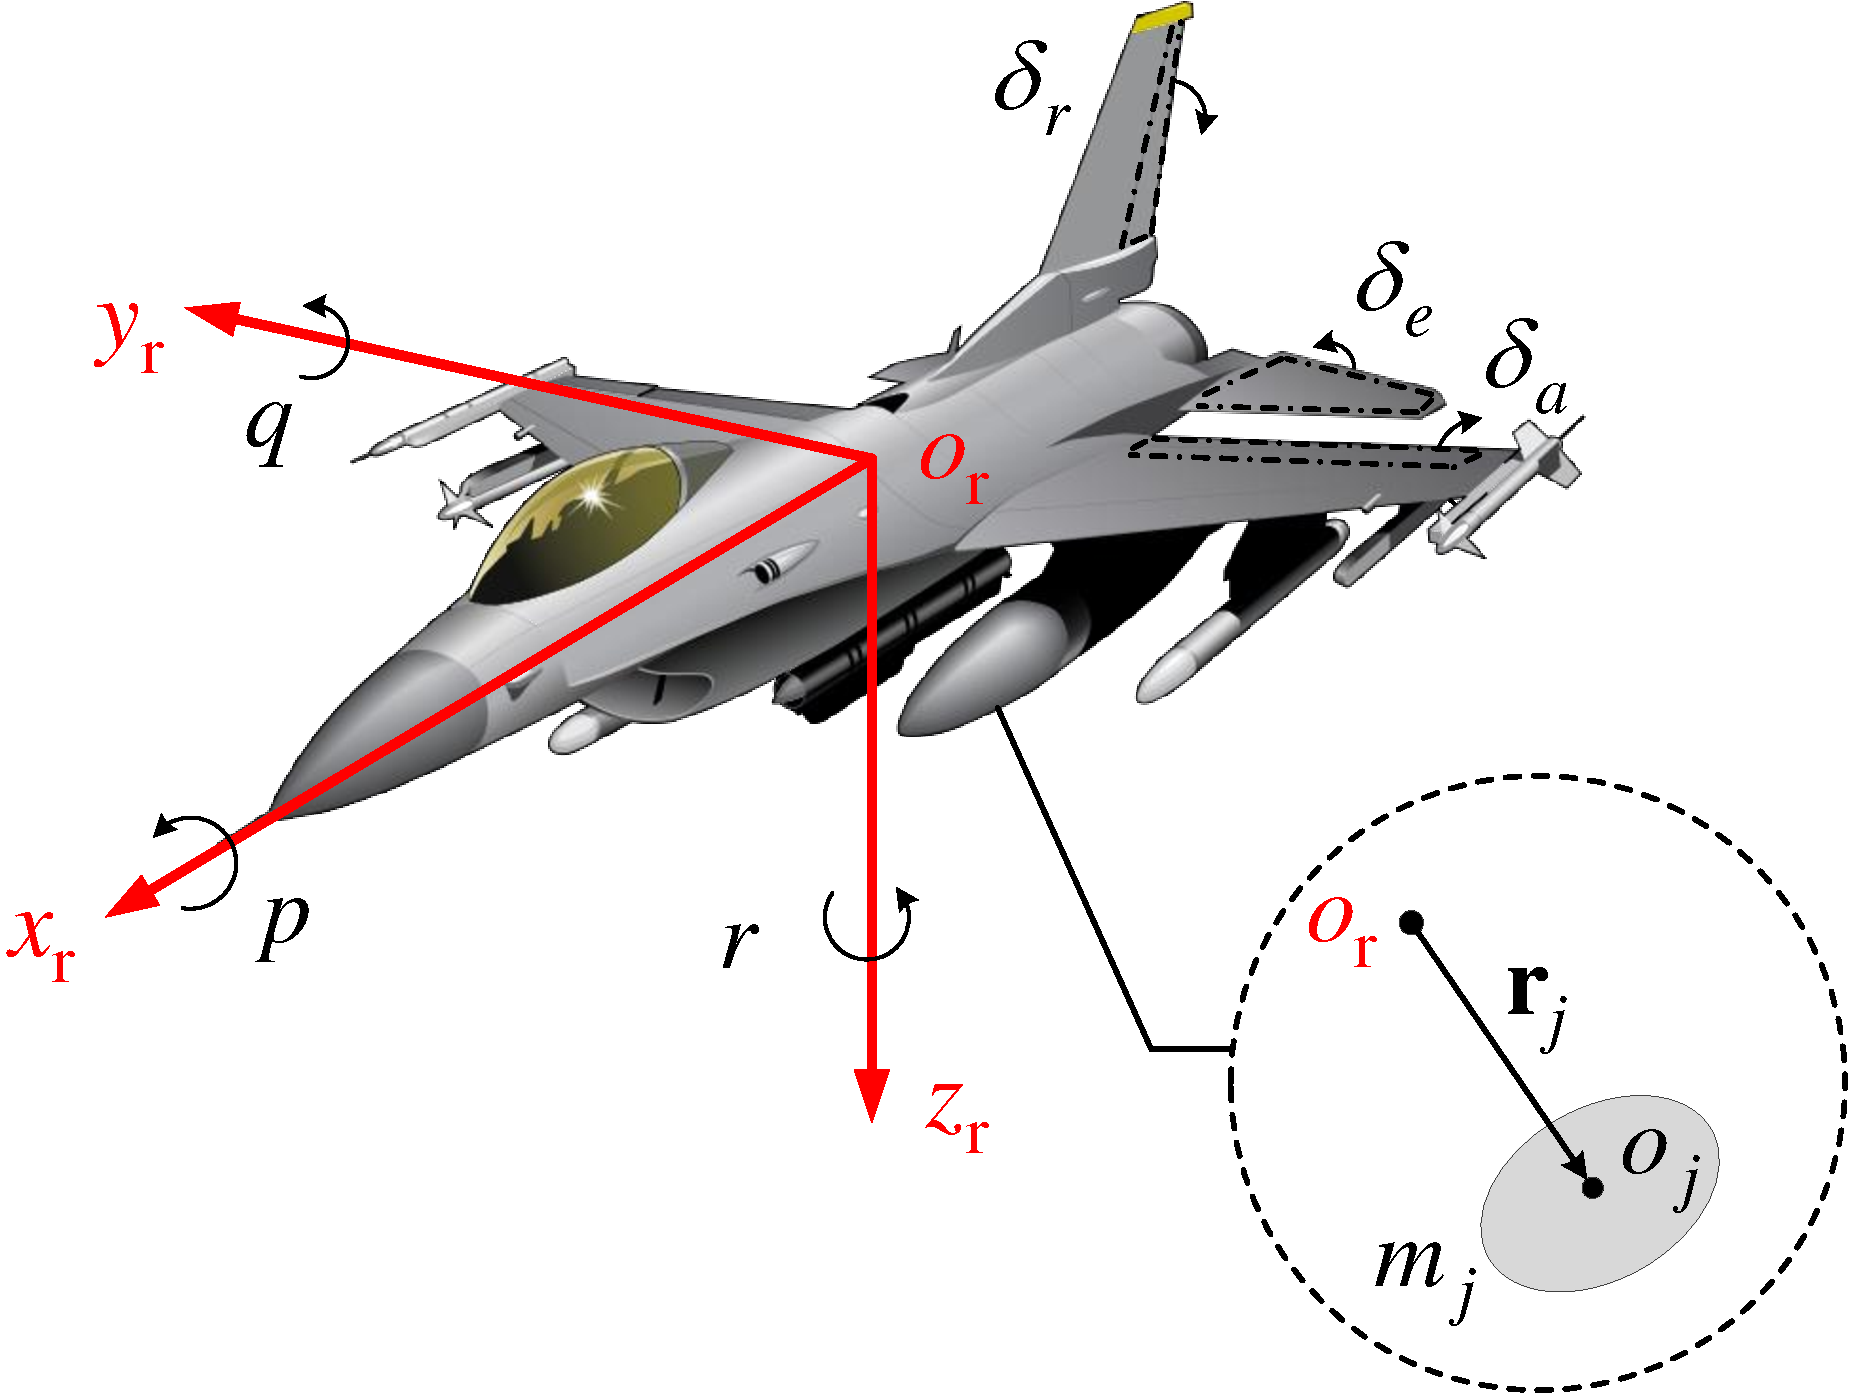
\includegraphics[width=0.5\textwidth]{Figures/Figs_Ch3/fig1.pdf}
	\caption{Schematic diagram of the F-16 refueling receiver}\label{fig4.1}
\end{figure}

\begin{itemize}	
	\item  
	Force Equations:
\end{itemize}


First, consider Eq. (\ref{eq4.1}). In order to establish the motion relationship of the receiver relative to the ground coordinate system, the velocity ${\mathbf{v}_{\rm{r}}}$ of the receiver is decomposed in the body coordinate system. In the body coordinate system, Eq. (\ref{eq4.1}) can be expressed as 
\begin{equation}\label{eq4.6}
\mathbf{F}^{\mathrm{b}}=\frac{\mathrm{d}}{\mathrm{d} t}\left(m \mathbf {v}_{\mathrm{r}}^{\mathrm{b}}\right)+\bm{\omega}_{\mathrm{r}}^{\mathrm{b}} \times m \mathbf{v}_{\mathrm{r}}^{\mathrm{b}}
\end{equation}
where $\mathbf{v}\mathrm{_r^b}$ is the velocity vector of the receiver’s center of gravity in the body coordinate system, and $\bm{\omega}\mathrm{_r^b}$ is the total angular velocity vector of the receiver relative to the ground coordinate system.

In the receiver body coordinate system, $\mathbf{v}\mathrm{_r^b}$ and $\bm{\omega}\mathrm{_r^b}$ can be decomposed into
\begin{equation}\label{eq4.7}
\mathbf{v}\mathrm{_r^b} = \mathbf{i}\mathrm{^b}u\mathrm{_r} + \mathbf{j}\mathrm{^b}v\mathrm{_r} + \mathbf{k}\mathrm{^b}w\mathrm{_r}
\end{equation}
\begin{equation}\label{eq4.8}
\bm{\omega}\mathrm{_r^b} = \mathbf{i}\mathrm{^b}p + \mathbf{j}\mathrm{^b}q + \mathbf{k}\mathrm{^b}r
\end{equation}
where $\mathbf{i}\mathrm{^b},\mathbf{j}\mathrm{^b}$ and $\mathbf{k}\mathrm{^b}$are the unit vectors of the $o\mathrm{_r}x\mathrm{_r}$-axis, $o\mathrm{_r}y\mathrm{_r}$-axis, and $o\mathrm{_r}z\mathrm{_r}$-axis of the receiver body coordinate system.

Therefore, the first term of Eq. (\ref{eq4.6}) can be expressed as
\begin{equation}\label{eq4.9}
\frac{\mathrm{d}}{\mathrm{d}t}\left( m\mathbf{v}\mathrm{_r^b} \right) = \dot{ m}\mathbf{v}\mathrm{_r^b} + m\dot{\mathbf{v}}\mathrm{_r^b} = \mathbf{i}\mathrm{^b}\left( {\dot mu\mathrm{_r} + m\dot{u}\mathrm{_r}} \right) + \mathbf{j}\mathrm{^b}\left( \dot mv\mathrm{_r} + m\dot{z}\mathrm{_r} \right) + \mathbf{k}\mathrm{^b}\left( \dot mw\mathrm{_r}+ m{\dot w}\mathrm{_r} \right)
\end{equation}
where $\dot{ m}$ is given by Eq. (\ref{eq4.4}). The second term of Eq. (\ref{eq4.6}) can be expressed as
\begin{equation}\label{eq4.10}
\bm{\omega}\mathrm{_r^b} \times m\mathbf{v}\mathrm{_r^b} = m\left| {\begin{array}{*{20}{c}}
	\mathbf{i}\mathrm{^b}&\mathbf{j}\mathrm{^b}&\mathbf{k}\mathrm{^b}\\
	p&q&r\\
	u\mathrm{_r}&v\mathrm{_r}&w\mathrm{_r}
	\end{array}} \right| = \mathbf{i}\mathrm{^b}m\left( w\mathrm{_r}q - v\mathrm{_r}r \right) + \mathbf{j}\mathrm{^b}m\left( u\mathrm{_r}r - w\mathrm{_r}p\right) + \mathbf{k}\mathrm{^b}m\left( v\mathrm{_r}p - u\mathrm{_r}q \right).
\end{equation}

%Decompose the external force $\mathbf{F}$ into body coordinate system
Represent $\mathbf{F}$ in the form of components in the body coordinate system as
\begin{equation}\label{eq4.11}
\mathbf{F}\mathrm{^b} = \mathbf{i}\mathrm{^b}F_{x}^\mathrm{b} + \mathbf{j}\mathrm{^b}F_y^\mathrm{b} + \mathbf{k}\mathrm{^b}F_z^\mathrm{b}.
\end{equation}
Therefore, substituting Eqs. (\ref{eq4.9}), (\ref{eq4.10}), and (\ref{eq4.11}) into Eq. (\ref{eq4.6}), one can obtain
\begin{equation}\label{eq4.12}
\begin{array}{l}
F_x^\mathrm{b} = m\left( \dot u\mathrm{_r} + w\mathrm{_r}q - v\mathrm{_r}r \right) + \dot mu\mathrm{_r}\\
F_y^\mathrm{b} = m\left( \dot v\mathrm{_r} + u\mathrm{_r}r - w\mathrm{_r}p \right) + \dot mv\mathrm{_r}\\
F_z^\mathrm{b} = m\left( \dot w\mathrm{_r} + v\mathrm{_r}p - u\mathrm{_r}q \right) + \dot mw\mathrm{_r} .
\end{array} 
\end{equation}
The total external force $\mathbf{F}$ includes gravity, aerodynamic force, and engine thrust. Assuming the engine thrust is $F_{T}$ and its direction is along the ${o_\mathrm{_r}}{x_\mathrm{_r}}$-axis of the body coordinate system. In the body coordinate system, the component of gravity is represented as follows
\begin{equation}\label{eq4.13}
\left[ \begin{array}{l}
G_x^\mathrm{b}\\
G_y^\mathrm{b}\\
G_z^\mathrm{b}
\end{array} \right] = \left[ \begin{array}{c}
- mg\sin \theta \\
mg\cos \theta \sin \phi \\
mg\cos \theta \cos \phi 
\end{array} \right]
\end{equation}
where $g$ is the gravitational acceleration. The aerodynamic force components along the three axes of the body coordinate system are denoted as $\bar{ X}, \bar{ Y}$ and $\bar{ Z}$, and their magnitudes are related to the receiver's airspeed ${V_\mathrm{r}}$, air density $\rho $, wing area $S$, wingspan $b$, angle of attack $\alpha $, sideslip angle $\beta $, and control surface deflection angle $	\boldsymbol{\delta}=[  {\delta}_{\rm{a}}  ,    {\delta}_{\rm{r}}   , {\delta}_{\rm{e}}  ,   {\delta}_{\rm{t}}  ]$, etc. The aerodynamic force components can be represented as follows
\begin{equation}\label{eq4.14}
\begin{array}{l}
\bar X = \bar qS{C_{{X_T}}}\left( {\alpha ,\beta ,p,q,r,\boldsymbol{\delta} ,...} \right)\\
\bar Y = \bar qS{C_{{Y_T}}}\left( {\alpha ,\beta ,p,q,r,\boldsymbol{\delta} ,...} \right)\\
\bar Z = \bar qS{C_{{Z_T}}}\left( {\alpha ,\beta ,p,q,r,\boldsymbol{\delta} ,...} \right)
\end{array}
\end{equation}
where $\bar q = 0.5\rho V_\mathrm{r}^2$ represents dynamic pressure, $S$ is the wing area, and the aerodynamic coefficients ${C_{{X_T}}},{C_{{Y_T}}}$ and ${C_{{Z_T}}}$ can be obtained from wind tunnel data or flight data. Interested readers can refer to reference \cite{nguyen_simulator_1979} for the specific forms of the aerodynamic coefficients.

Thus, the force equations for the receiver in the body coordinate system can be represented as follows
\begin{equation}\label{eq4.15}
\begin{array}{l}
{{\dot u}\mathrm{_r}} = r{v\mathrm{_r}} - q{w\mathrm{_r}} - g\sin \theta  + \frac{1}{m}\left( {\bar X + {F_T}} \right) - \frac{{\dot m{u\mathrm{_r}}}}{m}\\
{{\dot v}\mathrm{_r}} = p{w\mathrm{_r}} - r{u\mathrm{_r}} + g\sin \phi \cos \theta  + \frac{1}{m}\bar Y - \frac{{\dot m{v\mathrm{_r}}}}{m}\\
{{\dot w}\mathrm{_r}} = q{u\mathrm{_r}} - p{v\mathrm{_r}} + g\cos \phi \cos \theta  + \frac{1}{m}\bar Z - \frac{{\dot m{w\mathrm{_r}}}}{m}
\end{array}
\end{equation}

\begin{itemize}	
	\item  
	Moment Equations:
\end{itemize}

Considering Eq. (\ref{eq4.5}), let us decompose the angular momentum $\mathbf{L}\mathrm{_r^g}$ in the body coordinate system. In the body coordinate system, Eq. (\ref{eq4.5}) can be represented as follows
\begin{equation}\label{eq4.16}
\mathbf{M}\mathrm{^b} = \frac{\mathrm{d}\mathbf{L}\mathrm{_r^b}}{\mathrm{d}t} + \bm{\omega} \mathrm{_r^b} \times \mathbf{L}\mathrm{_r^b} .
\end{equation}
Assuming that the angular momentum $\mathbf{h}\mathrm{_E}$ generated by the engine thrust is in the direction of the positive $o\mathrm{_r}x\mathrm{_r}$-axis of the aircraft body, it can be represented in the body coordinate system as follows\cite{garza_collection_2003}
\begin{equation}\label{eq4.17}
\mathbf{h}\mathrm{_E^b} = {\left[ {\begin{array}{*{20}{c}}
		{{h_\mathrm{E}}}&0&0
		\end{array}} \right]\mathrm{^T}}
\end{equation}
where ${h_\mathrm{E}}$ is the magnitude of the angular momentum generated by the engine thrust. Therefore, the angular momentum can be represented in the body coordinate system as follows
\begin{equation}\label{eq4.18}
\mathbf{L}\mathrm{_r^b} = \mathbf{J}\bm{\omega}\mathrm{_r^b} + \mathbf{h}\mathrm{_E^b}
\end{equation}
where $\mathbf{J}$ is the inertia matrix of the receiver. Therefore, Eq. (\ref{eq4.16}) is represented as follows
\begin{equation}\label{eq4.19}
%	\begin{}{ll}
\begin{aligned}
\mathbf{M}\mathrm{^b} &= \frac{\mathrm{d}}{{\mathrm{d}t}}\left( \mathbf{J}\bm{\omega}\mathrm {_r^b} + \mathbf{h}\mathrm{_E^b} \right) + \bm{\omega}\mathrm{ _r^b} \times \left( {\mathbf{J}\bm{\omega}\mathrm {_r^b} + \mathbf{h}\mathrm{_E^b}} \right)\\
&= \dot{ \mathbf{J}}\bm{\omega}\mathrm{ _r^b} + \mathbf{J}\dot{ \bm{\omega}}\mathrm{ _r^b} + \bm{\omega}\mathrm{ _r^b} \times \left( \mathbf{J}\bm{\omega}\mathrm{ _r^b} + \mathbf{h}\mathrm{_E^b} \right) .
\end{aligned} 
\end{equation}

Based on Assumptions 2) and 4), it can be concluded that the rotational inertia $\mathbf{J}$ of the receiver consists of two parts: the rotational inertia $\mathbf{J}_{0}$ of the mechanical body and the rotational inertia $\mathbf{J}\mathrm{_f}$ of the fuel in the tank. According to Ref. \cite{waishek_derivation_2009}, the rotational inertia $\mathbf{J}\mathrm{_f}$ of the fuel in the tank is represented as follows
\begin{equation}\label{eq4.20}
\mathbf{J}\mathrm{_f}= \sum\limits_{j = 1}^k {{m_j}} \left( \mathbf{r}_{j}^\mathrm{T}{\mathbf{r}_j}{\mathbf{I}_3} - {\mathbf{r}_j}\mathbf{r}_{j}^\mathrm{T}\right)
\end{equation}
where $\mathbf{r}_{j} \in\mathbb{R}{^3}$ represents the vector from the center of mass ${o_j}$ of the fuel in the $j$th tank to the origin ${o_\text{r}}$ of the receiver's body coordinate system, and ${\mathbf{I}_3}$ represents the three-dimensional unit matrix. According to Assumption 5), ${\mathbf{r}_j}$ is constant; hence, we have 
\begin{equation}\label{eq4.21}
\dot{\mathbf{J}}\mathrm{_f} = \sum\limits_{j = 1}^k {{{\dot m}_j}} \left( \mathbf{r}_{j}^\mathrm{T}\mathbf{r}_{j}{\mathbf{I}_3} - \mathbf{r}_{j}\mathbf{r}_{j}^\mathrm{T} \right) .
\end{equation}
At a specific moment, the total rotational inertia of the receiver is given by 
\begin{equation}\label{eq4.22}
\mathbf{J} = {\mathbf{J}_0} + \mathbf{J}\mathrm{_f} = \left[ {\begin{array}{*{20}{c}}
	{{{J}_x}}&0&{ - {{J}_{xz}}}\\
	0&{{{J}_y}}&0\\
	{ - {{J}_{xz}}}&0&{{{J}_z}}
	\end{array}} \right] .
\end{equation}
Specifically, the rotational inertia of the mechanical body part of the receiver ${\bf{J}_0}$ is represented as follows 
\begin{equation}\label{eq4.23}
\mathbf{J}_{0} = \left[ {\begin{array}{*{20}{c}}
	{J_{x0}}&0&{ - {J_{xz0}}}\\
	0&{J_{y0}}&0\\
	{ - {J_{xz0}}}&0&{J_{z0}}
	\end{array}} \right] .
\end{equation}
Furthermore, according to Assumption 5), the positions of the fuel tanks and the distribution of fuel mass are symmetric. The rotational inertia $\mathbf{J}\mathrm{_f}$ is represented as follows
\begin{equation}\label{eq4.24}
\mathbf{J}_\text{f} = \left[ {\begin{array}{*{20}{c}}
	{J_{x1}}&0&{ - {J_{xz1}}}\\
	0&{J_{y1}}&0\\
	{ - {J_{xz1}}}&0&{J_{z1}}
	\end{array}} \right]
\end{equation}
where $J_{x0}$ and $J_{x1}$ represent the rotational inertia of the aircraft body and the fuel in the tanks around the $o\mathrm{_r}x\mathrm{_r}$-axis of the body, $J_{y0}$ and $J_{y1}$ represent the rotational inertia around the $o\mathrm{_r}y\mathrm{_r}$-axis, $J_{z0}$ and $J_{z1}$ represent the rotational inertia around the $o\mathrm{_r}z\mathrm{_r}$-axis, and  $J_{xz0}$ and $J_{xz1}$ represent the products of inertia. According to the symmetry assumption, the receiver is symmetric about the $o\mathrm{_r}x\mathrm{_r}z\mathrm{_r}$ plane of the body coordinate system, hence ${J_{xy}} \equiv {J_{yx}} \equiv {J_{yz}} \equiv {J_{zy}} = 0$. It is worth noting that $\bf{J}_{\rm{f}}$ is time-varying, by taking the derivative of Eq. (\ref{eq4.24}), it can be obtained
\begin{equation}\label{eq4.25}
\dot{\mathbf{J}}\mathrm{_{f}} = \left[ {\begin{array}{*{20}{c}}
	{{{\dot J}_{x1}}}&0&{ - {{\dot J}_{xz1}}}\\
	0&{{{\dot J}_{y1}}}&0\\
	{ - {{\dot J}_{xz1}}}&0&{{{\dot J}_{z1}}}
	\end{array}} \right]
\end{equation}
where the values of each element are dependent on the changes of the receiver's fuel tank mass. Since the rotational inertia $\mathbf{J}_{0}$ of the receiver's mechanical body part is constant, 
\begin{equation}\label{eq4.26}
\dot{\mathbf{J}} = {\dot{\mathbf{J}}_0} + {\dot{\mathbf{J}}\mathrm{_{f}}} = {\dot{\mathbf{J}}\mathrm{_{f}}} .
\end{equation}

The total external moment $\mathbf{M}\mathrm{^b}$ includes the aerodynamic moment $\mathbf{M}\mathrm{^{b}_{a}}$ and the moment $\mathbf{M}\mathrm{^{b}_{f}}$ generated by the gravity of the fuel in the tanks, satisfying the following equation
\begin{equation}\label{eq4.27}
\mathbf{M}\mathrm{^b} = \mathbf{M}\mathrm{^{b}_{a}} + \mathbf{M}\mathrm{^{b}_{f}}
\end{equation}
where the moment $\mathbf{M}\mathrm{^{b}_{f}}$ generated by the gravity of the fuel in the tanks can be represented as follows
\begin{equation}\label{eq4.28}
\mathbf{M}\mathrm{^{b}_{f}} = \sum\limits_{j = 1}^k \mathbf{r}_{j}  \times \mathbf{R}_{\rm{b/g}}\mathbf{G}_{j} = {\mathbf{i}^{\rm{b}}}{\bar L_f} + {\mathbf{j}^{\rm{b}}}{\bar M_f} + {\mathbf{k}^b}{\bar N_f}
\end{equation}
where $\mathbf{G}_{j} = {\left[ {\begin{array}{*{20}{c}}
		0&0&{{m_j}g}
		\end{array}} \right]^{\rm{T}}}$ represents the gravitational vector of the fuel in the $j$th tank, and $\bar{L}_{f}$, $\bar{ M}_{f}$, and $\bar{ N}_{f}$ respectively represent the magnitudes of the components of the moment generated by the gravity of the fuel in the tanks along the three axes of the receiver's body coordinate system. The aerodynamic moment $\mathbf{M}\mathrm{^{b}_{a}}$ can be decomposed into the body coordinate axes as follows
\begin{equation}\label{eq4.29}
\mathbf{M}\mathrm{^{b}_{a}} = {\mathbf{i}^{\rm{b}}}{\bar L_a} + {\mathbf{j}^{\rm{b}}}{\bar M_a} + {\mathbf{k}^{\rm{b}}}{\bar N_a}
\end{equation}
where ${\bar L_a}$, ${\bar M_a}$, and ${\bar N_a}$ represent the magnitudes of the components of the aerodynamic moment of the receiver along the three axes of its body coordinate system. Similar to the aerodynamic force, their magnitudes are related to the receiver's airspeed ${V_a}$, air density $\rho $, wing area $S$, wingspan $b$, angle of attack $\alpha $, sideslip angle $\beta $, and control surface deflection angle $\boldsymbol{\delta} $, etc. The specific forms can be represented as follows
\begin{equation}\label{4.30}
\begin{array}{l}
{{\bar L}_a} = \bar qSb{C_{{l_T}}}\left( {\alpha ,\beta ,p,q,r,\boldsymbol{\delta} ,...} \right)\\
{{\bar M}_a} = \bar qS\bar c{C_{{m_T}}}\left( {\alpha ,\beta ,p,q,r,\boldsymbol{\delta} ,...} \right)\\
{{\bar N}_a} = \bar qSb{C_{{n_T}}}\left( {\alpha ,\beta ,p,q,r,\boldsymbol{\delta} ,...} \right)
\end{array}
\end{equation}
where $\bar q = 0.5\rho V_\mathrm{r}^2$ represents dynamic pressure, $b$ is the wingspan, and $S$ is the wing area. The aerodynamic coefficients ${C_{{l_T}}},{C_{{m_T}}}$ and ${C_{{n_T}}}$ can be obtained from wind tunnel data or flight data. Interested readers can refer to Ref. \cite{nguyen_simulator_1979} to understand the specific forms of the aerodynamic coefficients.

According to Eqs. (\ref{eq4.28}) and (\ref{eq4.29}), Eq. (\ref{eq4.27}) can be redefined as follows
\begin{equation}\label{eq4.31}
\mathbf{M}\mathrm{^b} = {\mathbf{i}\mathrm{^b}}\bar L + {\mathbf{j}\mathrm{^b}}\bar M + {\mathbf{k}\mathrm{^b}}\bar N = {\mathbf{i}\mathrm{^b}}\left( {{{\bar L}_f} + {{\bar L}_a}} \right) + {\mathbf{j}\mathrm{^b}}\left( {{{\bar M}_f} + {{\bar M}_a}} \right) + {\mathbf{k}\mathrm{^b}}\left( {{{\bar N}_f} + {{\bar N}_a}} \right)
\end{equation}
Furthermore, Eq. (\ref{eq4.19}) is expressed as follows
\begin{equation}\label{eq4.32}
\begin{aligned}
\mathbf{M}^{\mathrm{b}} & =\frac{\mathrm{d}}{\mathrm{d} t}\left(\mathbf{J} \boldsymbol{\omega}_{\mathrm{r}}^{\mathrm{b}}+\mathbf{h}_{\mathrm{E}}^{\mathrm{b}}\right)+\boldsymbol{\omega}_{\mathrm{r}}^{\mathrm{b}} \times\left(\mathbf{J} \boldsymbol{\omega}_{\mathrm{r}}^{\mathrm{b}}+\mathbf{h}_{\mathrm{E}}^{\mathrm{b}}\right) \\
& =\mathbf{J} \boldsymbol{\omega}_{\mathrm{r}}^{\mathrm{b}}+\mathbf{J} \boldsymbol{\omega}_{\mathrm{r}}^{\mathrm{b}}+\boldsymbol{\omega}_{\mathrm{r}}^{\mathrm{b}} \times\left(\mathbf{J} \boldsymbol{\omega}_{\mathrm{r}}^{\mathrm{b}}+\mathbf{h}_{\mathrm{E}}^{\mathrm{b}}\right) \\
& =\underbrace{\mathbf{J}_0 \boldsymbol{\omega}_{\mathrm{r}}^{\mathrm{b}}+\boldsymbol{\omega}_{\mathrm{r}}^{\mathrm{b}} \times\left(\mathbf{J}_0 \boldsymbol{\omega}_{\mathrm{r}}^{\mathrm{b}}+\mathbf{h}_{\mathrm{E}}^{\mathrm{b}}\right)}_{\rm{Constant mass section \atop(mechanical body section)}}+\underbrace{\mathbf{J}_{\mathrm{f}} \dot{\omega}_{\mathrm{r}}^{\mathrm{b}}+\mathbf{J}_{\mathrm{f}} \boldsymbol{\omega}_{\mathrm{r}}^{\mathrm{b}}+\boldsymbol{\omega}_{\mathrm{r}}^{\mathrm{b}} \times\left(\mathbf{J}_{\mathrm{f}} \boldsymbol{\omega}_{\mathrm{r}}^{\mathrm{b}}\right)}_{\rm{Variable mass section \atop(fuel tank section)}} .
\end{aligned} 
\end{equation}
%\begin{equation}\label{eq4.32}
%	\begin{array}{c}
%		{\bf{M}^{\rm{b}}} = \frac{d}{{dt}}\left( {\bf{J}\bf{\omega} _{\rm{r}}^{\rm{b}} + \bf{h}_{\rm{E}}^{\rm{b}}} \right) + \omega _{\rm{r}}^{\rm{b}} \times \left( {\bf{J}\bf{\omega} _{\rm{r}}^{\rm{b}} + \bf{h}_{\rm{E}}^{\rm{b}}} \right)\\
%		 = \dot {\bf{J}}\omega _{\rm{r}}^{\rm{b}} + \bf{J}\dot {\omega} _{\rm{r}}^{\rm{b}} + \omega _{\rm{r}}^{\rm{b}} \times \left( {\bf{J}\omega _{\rm{r}}^{\rm{b}} + \bf{h}_{\rm{E}}^{\rm{b}}} \right)\\
%		 = \underbrace{{\bf{J}_{0}}\dot{ \omega} _{\rm{r}}^{\rm{b}} + \omega _{\rm{r}}^{\rm{b}} \times \left( {{\bf{J}_{0}}\omega _{\rm{r}}^{\rm{b}} + \bf{h}_{\rm{E}}^{\rm{b}}} \right)}_{\rm{Constant mass section (mechanical body section)}} +\underbrace{{\bf{J}_f}\dot \omega _{\rm{r}}^{\rm{b}} + {{\dot {\bf{J}}}_f}\omega _{\rm{r}}^{\rm{b}} + \omega _{\rm{r}}^{\rm{b}} \times \left( {{\bf{J}_{\rm{f}}}\omega _{\rm{r}}^{\rm{b}}} \right)}_{\rm{Variable mass section (fuel tank section)}} 
%		\end{array}
%\end{equation}
So far, we have decomposed the moment equation of the variable-mass aircraft model into two parts: the first part represents the constant-mass portion of the aircraft's mechanical body, and the second part represents the variable-mass portion due to the fuel in the tanks. The advantage of this approach is that it facilitates the analysis of the impact of fuel mass changes on the receiver's system.

Next, the moment equation represented by Eq. (\ref{eq4.32}) will be expanded into scalar form. From Eq. (\ref{eq4.18}), we have
\begin{equation}\label{4.33}
\mathbf{L}\mathrm{_r^b} = \left[ {\begin{array}{*{20}{c}}
	{{L_x}}\\
	{{L_y}}\\
	{{L_z}}
	\end{array}} \right] = \left[ {\begin{array}{*{20}{c}}
	{p{J_x} - r{J_{xz}} + {h_E}}\\
	{q{J_y}}\\
	{r{J_z} - p{J_{xz}}}
	\end{array}} \right]
\end{equation}
so
\begin{equation}\label{eq4.34}
\bm{\omega}\mathrm{_r^b} \times \mathbf{L}\mathrm{_r^b} = \left| {\begin{array}{*{20}{c}}
	{{\mathbf{i}\mathrm{^b}}}&{\mathbf{j}\mathrm{^b}}&{\mathbf{k}\mathrm{^b}}\\
	p&q&r\\
	{{L_x}}&{{L_y}}&{{L_z}}
	\end{array}} \right| = {\mathbf{i}\mathrm{^b}}\left( {q{L_z} - r{L_y}} \right) + {\mathbf{j}\mathrm{^b}}\left( {r{L_x} - p{L_z}} \right) + {\mathbf{k}\mathrm{^b}}\left( {p{L_y} - q{L_x}} \right) .
\end{equation}
As a result, it can be obtained
\begin{equation}\label{eq4.35}
\mathbf{J}\dot{\bm{\omega}}\mathrm{_r^b} + \bm{\omega}\mathrm{_r^b} \times \left( {\mathbf{J}\bm{\omega}\mathrm{_r^b} +\mathbf{ h}\mathrm{_E^b}} \right) = \left[ {\begin{array}{*{20}{c}}
	{\dot p{J_x} - \dot r{J_{xz}} + q\left( {r{J_z} - p{J_{xz}}} \right) - qr{J_y}}\\
	{\dot q{J_y} + r\left( {p{J_x} - r{J_{xz}} + {h_E}} \right) - p\left( {r{J_z} - p{J_{xz}}} \right)}\\
	{ - \dot p{J_{xz}} + \dot r{J_z} + pq{J_y} - q\left( {p{J_x} - r{J_{xz}} + {h_E}} \right)}
	\end{array}} \right] .
\end{equation}
According to Eq. (\ref{eq4.25}), one can obtain
\begin{equation}\label{eq4.36}
{\dot{ \mathbf{J}}\mathrm{_f}}{\bm{\omega}\mathrm{_r}} = \left[ {\begin{array}{*{20}{c}}
	{p{{\dot J}_{x1}} - r{{\dot J}_{xz1}}}\\
	{q{{\dot J}_{y1}}}\\
	{r{{\dot J}_{z1}} - p{{\dot J}_{xz1}}}
	\end{array}} \right] .
\end{equation}
Therefore, based on Eqs. (\ref{eq4.31}), (\ref{eq4.32}), (\ref{eq4.35}), and (\ref{eq4.36}), one can obtain
\begin{equation}\label{eq4.37}
\left\{ \begin{array}{l}
\bar L{\rm{ = }}\dot p{J_x} - \dot r{J_{xz}} + qr\left( {{J_z} - {J_y}} \right) - pq{J_{xz}} + p{{\dot J}_{x1}} - r{{\dot J}_{xz1}}\\
\bar M{\rm{ = }}\dot q{J_y} + pr\left( {{J_x} - {J_z}} \right) + \left( {{p^2} - {r^2}} \right){J_{xz}} + r{h_E} + q{{\dot J}_{y1}}\\
\bar N{\rm{ = }}\dot r{J_z} - \dot p{J_{xz}} + pq\left( {{J_y} - {J_x}} \right) + qr{J_{xz}} - q{h_E} + r{{\dot J}_{z1}} - p{{\dot J}_{xz1}}\, .
\end{array} \right .
\end{equation}
By rearranging Eq. (\ref{eq4.37}), the moment equations of the receiver in the body coordinate system can be obtained
\begin{equation}\label{eq4.38}
\begin{array}{l}
\dot p = \left( {{c_1}r + {c_2}p} \right)q + {c_3}\bar L + {c_4}\left( {\bar N + {h_E}q} \right) + {\kappa _1}p + {\kappa _2}r\\
\dot q = {c_5}pr - {c_6}\left( {{p^2} - {r^2}} \right) + {c_7}\left( {\bar M - {h_E}r} \right) + {\kappa _3}q\\
\dot r = \left( {{c_8}p - {c_2}r} \right)q + {c_4}\bar L + {c_9}\left( {\bar N + {h_E}q} \right) + {\kappa _4}p - {\kappa _5}r\, .
\end{array}
\end{equation}
where the specific expressions of each coefficient are as follows
\[\begin{array}{l}
{c_1} = \frac{{\left( {{J_y} - {J_z}} \right){J_z} - J_{xz}^2}}{\Sigma },{c_2} = \frac{{\left( {{J_x} - {J_y} + {J_z}} \right){J_{xz}}}}{\Sigma },{c_3} = \frac{{{J_z}}}{\Sigma },{c_4} = \frac{{{J_{xz}}}}{\Sigma },{c_5} = \frac{{{J_z} - {J_x}}}{{{J_y}}},{c_6} = \frac{{{J_{xz}}}}{{{J_y}}},\\
{c_7} = \frac{1}{{{J_y}}},{c_8} = \frac{{{J_x}\left( {{J_x} - {J_y}} \right) + J_{xz}^2}}{\Sigma },{c_9} = \frac{{{J_x}}}{\Sigma },{\kappa _1} = \frac{{{{\dot J}_{xz1}}{J_{xz}} - {{\dot J}_{x1}}{J_z}}}{\Sigma },{\kappa _2} = \frac{{{{\dot J}_{xz1}}{J_z} - {{\dot J}_{z1}}{J_{xz}}}}{\Sigma },{\kappa _3} = \frac{{{{\dot J}_{y1}}}}{{{J_y}}},\\
{\kappa _4} = \frac{{{{\dot J}_{x1}}{J_{xz}} - {J_x}{{\dot J}_{zx1}}}}{\Sigma },{\kappa _5} = \frac{{{J_{x1}}{{\dot J}_z} - {{\dot J}_{xz1}}{J_{xz}}}}{\Sigma }.\Sigma  = {J_x}{J_z} - J_{xz}^2\, .
\end{array}\]


\begin{itemize}	
	\item  
	Motion Equations:
\end{itemize}

According to Section 2.3.1.4, there exists the following relationship between the attitude angles and the body angular velocities
\begin{equation}\label{eq4.39}
\left[ {\begin{array}{*{20}{c}}
	{\dot \phi }\\
	{\dot \theta }\\
	{\dot \psi }
	\end{array}} \right] = \left[ {\begin{array}{*{20}{c}}
	1&{\tan \theta \sin \phi }&{\tan \theta \cos \phi }\\
	0&{\cos \phi }&{ - \sin \phi }\\
	0&{\sin \phi /cos\theta} &{\cos \phi/cos\theta } 
	\end{array}} \right] \left[ {\begin{array}{*{20}{c}}
	p\\
	q\\
	r
	\end{array}} \right]
\end{equation}
Therefore, the equations of motion for the receiver can be obtained as follows
\begin{equation}\label{eq4.40}
\begin{array}{l}
\dot \phi  = p + \tan \theta \left( {q\sin \phi  + r\cos \phi } \right)\\
\dot \theta  = q\cos \phi  - r\sin \phi \\
\dot \psi  = \frac{{q\sin \phi  + r\cos \phi }}{{\cos \theta }}
\end{array}
\end{equation}
The equation above can also be derived from the relationship between the derivative of the direction cosine matrix and the body angular velocity, which is $\dot{\mathbf{ R}}\mathrm{_{g/b}} = \mathbf{ R}\mathrm{_{g/b}}\left[ \bm{\omega}\mathrm{^b}\right]_ \times$.

\begin{itemize}	
	\item  
	Navigation Equations:
\end{itemize}


The position of the receiver in the ground coordinate system is represented as $\mathbf{p}\mathrm{_r^g} \triangleq  {\left[ \begin{array}{*{20}{c}}
	x\mathrm{_r}&y\mathrm{_r}&h\mathrm{_r}\end{array} \right]^{\mathrm{T}}}$. 
Based on the relationship between position and velocity, one can obtain the velocity vector in the ground coordinate system as 
$\mathbf{v}\mathrm{_r^g} = \dot{\bf{p}}\mathrm{_r^g} = {\left[ {\begin{array}{*{20}{c}}{{{\dot x}\mathrm{_r}}}&{{{\dot y}\mathrm{_r}}}&{{{\dot h}\mathrm{_r}}}\end{array}} \right]^{\mathrm{T}}}$.
In the body coordinate system, the velocity vector of the receiver is represented as $\mathbf{v}\mathrm{_r^b} \triangleq {\left[ {\begin{array}{*{20}{c}}{{{ u}\mathrm{_r}}}&{{{v}\mathrm{_r}}}&{{{ w}\mathrm{_r}}}\end{array}} \right]^{\mathrm{T}}}$. 
By using the transformation relationship between the ground coordinate system and the body coordinate system, which is $\mathbf{v}\mathrm{_r^g} = {{\bf{R}}\mathrm{_{g/b}}}\left( {\theta ,\psi ,\phi } \right)\bf{v}\mathrm{_r^b}$, one can derive the navigation equations for the receiver as follows	
\begin{equation}\label{eq4.41}
\begin{aligned}
& \dot{x}_{\mathrm{r}}=u_{\mathrm{r}} \cos \psi \cos \theta+v_{\mathrm{r}}(\cos \psi \sin \theta \sin \phi-\sin \psi \cos \phi)+w_{\mathrm{r}}(\cos \psi \sin \theta \cos \phi+\sin \psi \sin \phi) \\
& \dot{y}_{\mathrm{r}}=u_{\mathrm{r}} \sin \psi \cos \theta+v_{\mathrm{r}}(\sin \psi \sin \theta \sin \phi+\cos \psi \cos \phi)+w_{\mathrm{r}}(\sin \psi \sin \theta \cos \phi-\cos \psi \sin \theta) \\
& \dot{h}_{\mathrm{r}}=u_{\mathrm{r}} \sin \theta-v_{\mathrm{r}} \cos \theta \sin \phi-w_{\mathrm{r}} \cos \theta \cos \phi \, .
\end{aligned}
\end{equation}
%\begin{equation}\label{eq4.41}
%	\begin{array}{c}
%		{{\dot x}_{\mathrm{r}}} = {u_{\mathrm{r}}}\cos \psi \cos \theta  + {v_{\mathrm{r}}}\left( {\cos \psi \sin \theta \sin \phi  - \sin \psi \cos \phi } \right) + {w_{\mathrm{r}}}\left( {\cos \psi \sin \theta \cos \phi  + \sin \psi \sin \phi } \right)\\
%		{{\dot y}_{\mathrm{r}}} = {u_{\mathrm{r}}}\sin \psi \cos \theta  + {v_{\mathrm{r}}}\left( {\sin \psi \sin \theta \sin \phi  + \cos \psi \cos \phi } \right) + {w_{\mathrm{r}}}\left( {\sin \psi \sin \theta \cos \phi  - \cos \psi \sin \theta } \right)\\
%		{{\dot h}_{\mathrm{r}}} = {u_{\mathrm{r}}}\sin \theta  - {v_{\mathrm{r}}}\cos \theta \sin \phi  - {w_{\mathrm{r}}}\cos \theta \cos \phi 
%		\end{array}
%\end{equation}

Untill now, the kinematic and dynamic equations of the receiver are established. The nonlinear model of the receiver consists of a total of twelve differential equations, including force equations, moment equations, motion equations, and navigation equations, given by Eqs. (\ref{eq4.15}), (\ref{eq4.38}), (\ref{eq4.40}), and (\ref{eq4.41}). Based on these equations, receiver 6-DOF motion equations are presented as follows:

Force equations 
\begin{equation}\label{eq4.42}
\begin{aligned}
& \dot{u}_{\mathrm{r}}=r v_{\mathrm{r}}-q w_{\mathrm{r}}-g \sin \theta+\frac{1}{m}\left(\bar{X}+F_T\right)-\frac{\dot{m} u_{\mathrm{r}}}{m} \\
& \dot{v}_{\mathrm{r}}=p w_{\mathrm{r}}-r u_{\mathrm{r}}+g \sin \phi \cos \theta+\frac{1}{m} \bar{Y}-\frac{\dot{m} v_{\mathrm{r}}}{m} \\
& \dot{w}_{\mathrm{r}}=q u_{\mathrm{r}}-p v_{\mathrm{r}}+g \cos \phi \cos \theta+\frac{1}{m} \bar{Z}-\frac{\dot{m} w_{\mathrm{r}}}{m}
\end{aligned}
\end{equation}
%\begin{equation}\label{eq4.42}
%		 \begin{array}{c}
%			{{\dot u}_{\mathrm{r}}} = r{v_{\mathrm{r}}} - q{w_{\mathrm{r}}} - g\sin \theta  + \frac{1}{m}\left( {\bar X + {F_T}} \right) - \frac{{\dot m{u_{\mathrm{r}}}}}{m}\\
%			{{\dot v}_{\mathrm{r}}} = p{w_{\mathrm{r}}} - r{u_{\mathrm{r}}} + g\sin \phi \cos \theta  + \frac{1}{m}\bar Y - \frac{{\dot m{v_{\mathrm{r}}}}}{m}\\
%			{{\dot w}_{\mathrm{r}}} = q{u_{\mathrm{r}}} - p{v_{\mathrm{r}}} + g\cos \phi \cos \theta  + \frac{1}{m}\bar Z - \frac{{\dot m{w_{\mathrm{r}}}}}{m}
%			\end{array}
%\end{equation}

Moment equations 
\begin{equation}\label{eq4.43}
\begin{aligned}
& \dot{p}=\left(c_1 r+c_2 p\right) q+c_3 \bar{L}+c_4\left(\bar{N}+h_E q\right)+\kappa_1 p+\kappa_2 r \\
& \dot{q}=c_5 p r-c_6\left(p^2-r^2\right)+c_7\left(\bar{M}-h_E r\right)+\kappa_3 q \\
& \dot{r}=\left(c_8 p-c_2 r\right) q+c_4 \bar{L}+c_9\left(\bar{N}+h_E q\right)+\kappa_4 p-\kappa_5 r
\end{aligned}
\end{equation}
%\begin{equation}\label{eq4.43}	
%		  \begin{array}{c}
%				\dot p = \left( {{c_1}r + {c_2}p} \right)q + {c_3}\bar L + {c_4}\left( {\bar N + {h_E}q} \right) + {\kappa _1}p + {\kappa _2}r\\
%				\dot q = {c_5}pr - {c_6}\left( {{p^2} - {r^2}} \right) + {c_7}\left( {\bar M - {h_E}r} \right) + {\kappa _3}q\\
%				\dot r = \left( {{c_8}p - {c_2}r} \right)q + {c_4}\bar L + {c_9}\left( {\bar N + {h_E}q} \right) + {\kappa _4}p - {\kappa _5}r
%			\end{array}
%\end{equation}		 

Motion equations  
\begin{equation}\label{eq4.44}
\begin{aligned}
& \dot{\phi}=p+\tan \theta(q \sin \phi+r \cos \phi) \\
& \dot{\theta}=q \cos \phi-r \sin \phi \\
& \dot{\psi}=\frac{q \sin \phi+r \cos \phi}{\cos \theta}
\end{aligned}
\end{equation}
%\begin{equation}\label{eq4.44}
% \begin{array}{c}
%				\dot \phi  = p + \tan \theta \left( {q\sin \phi  + r\cos \phi } \right)\\
%				\dot \theta  = q\cos \phi  - r\sin \phi \\
%				\dot \psi  = \frac{{q\sin \phi  + r\cos \phi }}{{\cos \theta }}
%				\end{array}
%\end{equation}

Navigation equations  
\begin{equation}\label{eq4.45}
\begin{aligned}
& \dot{x}_{\mathrm{r}}=u_{\mathrm{r}} \cos \psi \cos \theta+v_{\mathrm{r}}(\cos \psi \sin \theta \sin \phi-\sin \psi \cos \phi)+w_{\mathrm{r}}(\cos \psi \sin \theta \cos \phi+\sin \psi \sin \phi) \\
& \dot{y}_{\mathrm{r}}=u_{\mathrm{r}} \sin \psi \cos \theta+v_{\mathrm{r}}(\sin \psi \sin \theta \sin \phi+\cos \psi \cos \phi)+w_{\mathrm{r}}(\sin \psi \sin \theta \cos \phi-\cos \psi \sin \theta) \\
& \dot{h}_{\mathrm{r}}=u_{\mathrm{r}} \sin \theta-v_{\mathrm{r}} \cos \theta \sin \phi-w_{\mathrm{r}} \cos \theta \cos \phi\, .
\end{aligned}
\end{equation}
%\begin{equation}\label{eq4.45}
%		\begin{array}{c}
%				{{\dot x}_{\mathrm{r}}} = {u_{\mathrm{r}}}\cos \psi \cos \theta  + {v_{\mathrm{r}}}\left( {\cos \psi \sin \theta \sin \phi  - \sin \psi \cos \phi } \right) + {w_{\mathrm{r}}}\left( {\cos \psi \sin \theta \cos \phi  + \sin \psi \sin \phi } \right)\\
%				{{\dot y}_{\mathrm{r}}} = {u_{\mathrm{r}}}\sin \psi \cos \theta  + {v_{\mathrm{r}}}\left( {\sin \psi \sin \theta \sin \phi  + \cos \psi \cos \phi } \right) + {w_{\mathrm{r}}}\left( {\sin \psi \sin \theta \cos \phi  - \cos \psi \sin \theta } \right)\\
%				{{\dot h}_{\mathrm{r}}} = {u_{\mathrm{r}}}\sin \theta  - {v_{\mathrm{r}}}\cos \theta \sin \phi  - {w_{\mathrm{r}}}\cos \theta \cos \phi 
%				\end{array}
%\end{equation}

Instead of ${u_\mathrm{r}},{v_\mathrm{r}},{w_\mathrm{r}}$, ${V_\mathrm{r}}, \alpha, \beta $ are also usually used to represent the force equations, where ${V_\mathrm{r}}$ is the airspeed magnitude of the receiver, and $\alpha$ and $\beta$ represent the angle of attack and sideslip angle, respectively. This is because in practical aircraft, $V_\mathrm{r},\alpha$ and $\beta$ can be directly measured, and they have a more direct relationship with aerodynamics, moments, and navigation. Ignoring wind disturbances, from Section 1.3.1.2, we know that there exists the following relationship among the velocity vector 
$\mathbf{v}\mathrm{_r^b} \triangleq {\left[ {\begin{array}{*{20}{c}}
		{{u\mathrm{_r}}}&{{v\mathrm{_r}}}&{{w\mathrm{_r}}}
		\end{array}} \right]^\mathrm{T}}$, airspeed $V_\mathrm{{r}}$, angle of attack $\alpha$, and sideslip angle $\beta$
\begin{equation}\label{eq4.46}
\begin{array}{l}
{u\mathrm{_r}} = {V_\mathrm{r}}\cos \alpha \cos \beta \\
{v\mathrm{_r}} = {V_\mathrm{r}}\sin \beta \\
{w\mathrm{_r}} = {V_\mathrm{r}}\sin \alpha \cos \beta 
\end{array}
\end{equation}
Taking its derivative, one can obtain
\begin{equation}\label{eq4.47}
\begin{array}{l}
{{\dot u}\mathrm{_r}} = {{\dot V}_\mathrm{r}}\cos \alpha \cos \beta  - \dot \alpha  \cdot {V_\mathrm{r}}\sin \alpha \cos \beta  - \dot \beta  \cdot {V_\mathrm{r}}\cos \alpha \sin \beta \\
{{\dot v}\mathrm{_r}} = {{\dot V}_\mathrm{r}}\sin \beta  + \dot \beta  \cdot {V_\mathrm{r}}\cos \beta \\
{w\mathrm{_r}} = {{\dot V}_\mathrm{r}}\sin \alpha \cos \beta  + \dot \alpha  \cdot {V_\mathrm{r}}\cos \alpha \cos \beta  - \dot \beta  \cdot {V_\mathrm{r}}\sin \alpha \sin \beta \, .
\end{array}
\end{equation}
Simultaneously, the following relationships exist
\begin{equation}\label{eq4.48}
\begin{aligned}
& V_{\mathrm{r}}=\left\|\bf{v}_{\mathrm{r}}\right\|=\sqrt{u_{\mathrm{r}}^2+v_{\mathrm{r}}^2+w_{\mathrm{r}}^2} \\
& \alpha=\tan ^{-1}\left(\frac{w_{\mathrm{r}}}{u_{\mathrm{r}}}\right) \\
& \beta=\sin ^{-1}\left(\frac{v_{\mathrm{r}}}{V_{\mathrm{r}}}\right)
\end{aligned}
\end{equation}
%\begin{equation}\label{eq4.48}
%	\begin{array}{l}
%		{V\mathrm{_r}} = \left\| {{v\mathrm{_r}}} \right\| = \sqrt {u\mathrm{_r}^2 + v\mathrm{_r}^2 + w\mathrm{_r}^2} {\rm{    }}\\
%		\alpha  = {\tan ^{ - 1}}\left( {\frac{{{w\mathrm{_r}}}}{{{u\mathrm{_r}}}}} \right){\rm{     }}\\
%		\beta  = {\sin ^{ - 1}}\left( {\frac{{{v\mathrm{_r}}}}{{{V\mathrm{_r}}}}} \right)
%		\end{array}
%\end{equation}
Taking its derivative, one can obtain
\begin{equation}\label{eq4.49}
\begin{aligned}
& \dot{V}_{\mathrm{r}}=\frac{u_{\mathrm{r}} \dot{u}_{\mathrm{r}}+v_{\mathrm{r}} \dot{v}_{\mathrm{r}}+w_{\mathrm{r}} \dot{w}_{\mathrm{r}}}{V_{\mathrm{r}}} \\
& \dot{\alpha}=\frac{u_{\mathrm{r}} \dot{w}_{\mathrm{r}}-w_{\mathrm{r}} \dot{u}_{\mathrm{r}}}{u_{\mathrm{r}}^2+w_{\mathrm{r}}^2} \\
& \dot{\beta}=\frac{V_{\mathrm{r}} \dot{v}_{\mathrm{r}}-v_{\mathrm{r}} \dot{V}_{\mathrm{r}}}{V_{\mathrm{r}}^2 \sqrt{1-\left(\frac{v_{\mathrm{r}}}{V_{\mathrm{r}}}\right)^2}}
\end{aligned}
\end{equation}
%\begin{equation}\label{eq4.49}
%	\begin{array}{l}
%		{{\dot V}\mathrm{_r}} = \frac{{{u\mathrm{_r}}{{\dot u}\mathrm{_r}} + {v\mathrm{_r}}{{\dot v}\mathrm{_r}} + {w\mathrm{_r}}{{\dot w}\mathrm{_r}}}}{{{V\mathrm{_r}}}}\\
%		\dot \alpha  = \frac{{{u\mathrm{_r}}{{\dot w}\mathrm{_r}} - {w\mathrm{_r}}{{\dot u}\mathrm{_r}}}}{{u\mathrm{_r}^2 + w\mathrm{_r}^2}}\\
%		\dot \beta  = \frac{{{V\mathrm{_r}}{{\dot v}\mathrm{_r}} - {v\mathrm{_r}}{{\dot V}\mathrm{_r}}}}{{V\mathrm{_r}^2\sqrt {1 - {{\left( {\frac{{{v\mathrm{_r}}}}{{{V\mathrm{_r}}}}} \right)}^2}} }}
%		\end{array}
%\end{equation}

The process of calculating ${\dot V_\mathrm{r}}$, $\dot \alpha $, and $\dot \beta $ is as follows: First, use Eq. (\ref{eq4.42}) to calculate ${\dot u\mathrm{_r}}$, ${\dot v\mathrm{_r}}$, and ${\dot w\mathrm{_r}}$. Then, use the current values of ${V_\mathrm{r}}$, $\alpha$, and $\beta$ (obtained from instruments) to calculate $u\mathrm{_{r}}$, $v\mathrm{_{r}}$, and $w\mathrm{_{r}}$ using Eq. (\ref{eq4.46}). Finally, substitute the obtained $u\mathrm{_{r}}$, $v\mathrm{_{r}}$, and $w\mathrm{_{r}}$ along with the current flight speed $V_\mathrm{{r}}$ into Eq. (\ref{eq4.49}) to get ${\dot V_\mathrm{r}}$, $\dot \alpha $, and $\dot \beta $. This method avoids the lengthy nonlinear calculation process when directly computing ${\dot V_\mathrm{r}}$, $\dot \alpha $, and $\dot \beta $ in the airflow coordinate system. It also allows the aircraft's dimensionless aerodynamic coefficients to be used directly in the body coordinate system without the need to convert the coefficients to the airflow coordinate system.
In general, the nonlinear model of the receiver consists of Eqs. (\ref{eq4.42}), (\ref{eq4.43}), (\ref{eq4.44}), and (\ref{eq4.45}). 

In practical applications, Eq. (\ref{eq4.49}) is commonly used instead of Eq. (\ref{eq4.42}). The new nonlinear model of the receiver consists of Eqs. (\ref{eq4.43}), (\ref{eq4.44}), (\ref{eq4.45}), and (\ref{eq4.49}), represented as a nonlinear state equation
\begin{equation}\label{eq4.50}
{\dot{\mathbf{x}}\mathrm{_r}} = \bm{f}\left( {{{\mathbf{x}}_{\rm{r}}},{\mathbf{u}_{\rm{r}}}} \right)
\end{equation}
where the state variables are represented by ${\mathbf{x}\mathrm{_r}} \triangleq {\left[ {\begin{array}{*{20}{c}}
		{{x\mathrm{_r}}}&{{y\mathrm{_r}}}&{{h\mathrm{_r}}}&\phi &\theta &\psi &{{V_\mathrm{r}}}&\alpha &\beta &p&q&r
		\end{array}} \right]^\mathrm{T}}$, which includes position, attitude angles, aerodynamic angles, and angular velocities. The control inputs are represented by ${\mathbf{u}_\mathrm{r}} \triangleq {\left[ {\begin{array}{*{20}{c}}
		{{\delta _\mathrm{t}}}&{{\delta _\mathrm{e}}}&{{\delta _\mathrm{a}}}&{{\delta _\mathrm{r}}}
		\end{array}} \right]^\mathrm{T}}$, which includes throttle, elevator, aileron, and rudder operations.

\subsection{Nonlinear Model Decoupling and Linearization}
\subsubsection{Decoupling}

For the receiver, during the refueling process, it maintains a slightly pitched-up level flight attitude. This state satisfies horizontal no sideslip flight condition, which means that the roll angle and sideslip angle satisfy $\phi  = \beta  \equiv 0$, and the angle of attack $\alpha$, yaw angle $\gamma$, and pitch angle $\theta$ satisfy $\theta  = \gamma  + \alpha $, while $\dot \theta  = q$ simultaneously.

In the body coordinate system, gravity is given by Eq. (\ref{eq4.13}). When transformed into the airflow coordinate system, it can be obtained
\begin{equation}\label{eq4.51}
\left[ \begin{array}{l}
G_x^\mathrm{w}\\
G_y^\mathrm{w}\\
G_z^\mathrm{w}
\end{array} \right] = \left[ \begin{array}{c}
mg\left( { - \cos \alpha \cos \beta \sin \theta  + \sin \beta \sin \phi \cos \theta  + \sin \alpha \cos \beta \cos \phi \cos \theta } \right)\\
mg\left( {\cos \alpha \sin \beta \sin \theta  + \cos \beta \sin \phi \cos \theta  - \sin \alpha \sin \beta \cos \phi \cos \theta } \right)\\
mg\left( {\sin \alpha \sin \theta  + \cos \alpha \cos \phi \cos \theta } \right)
\end{array} \right]
\end{equation}

Considering in the airflow coordinate system, the aerodynamic lift of the receiver is denoted as $L$, the aerodynamic drag as $D$, and the side force as $Y$. According to the transformation relationship between the body coordinate system and the airflow coordinate system, one have
\begin{equation}\label{eq4.52}
{\left[ \begin{array}{l}
	{\bar X}\\
	{\bar Y}\\
	{\bar Z}
	\end{array} \right]_\text{body}} = {\left[ \begin{array}{c}
	{F_T}\\
	0\\
	0
	\end{array} \right]_\text{body}} + {{\bf{R}}_{{\rm{b/w}}}}\left( {\alpha ,\beta } \right){\left[ \begin{array}{c}
	- D\\
	Y\\
	- L
	\end{array} \right]_\text{wind}}
\end{equation}
which can be expanded as
\begin{equation}\label{eq4.53}
\begin{array}{l}
\bar X = {F_T} + L\sin \alpha  - Y\cos \alpha \sin \beta  - D\cos \alpha \cos \beta \\
\bar Y = Y\cos \beta  - D\sin \beta \\
\bar Z =  - L\cos \alpha  - Y\sin \alpha \sin \beta  - D\sin \alpha \cos \beta 
\end{array}
\end{equation}
Therefore, based on Eqs. (\ref{eq4.47}), (\ref{eq4.51}), and (\ref{eq4.53}), Eq. (\ref{eq4.42}) can be transformed into
\begin{equation}\label{eq4.54}
\begin{array}{l}
m{{\dot V}_\mathrm{r}} = {F_T}\cos \alpha \cos \beta  - D + G_x^\mathrm{w} - \dot m{V_\mathrm{r}}\\
m{V_\mathrm{r}}\dot \beta  =  - {F_T}\cos \alpha \sin \beta  + Y - m{V_\mathrm{r}}\left( { - p\sin \alpha  + r\cos \alpha } \right) + G_y^\mathrm{w}\\
m{V_\mathrm{r}}\cos \beta \dot \alpha =  - {F_T}\sin \alpha  - L + m{V_\mathrm{r}}\left( { - p\cos \alpha \sin \beta  + q\cos \beta  - r\sin \alpha \sin \beta } \right) + G_z^\mathrm{w}
\end{array}
\end{equation}
By using the condition $p = r \equiv 0$, the second equation in the moment equation group (\ref{eq4.43}) can be simplified to
\begin{equation}\label{eq4.55}
\dot q = {c_7}\bar M - {\kappa _3}q \, .
\end{equation}

Combining with Eq. (\ref{eq4.54}) and utilizing the horizontal no sideslip flight condition $\phi  = \beta  \equiv 0$ and $p = r \equiv 0$, the motion equations of the receiver can be decoupled into longitudinal motion that does not depend on lateral-directional states.

(1) The longitudinal motion equations are as follows
\begin{equation}\label{eq4.56}
\left\{ \begin{array}{l}
m{{\dot V}_\text{r}} = {F_T}\cos \alpha  - D - mg\left( {\cos \alpha \sin \theta  - \sin \alpha \cos \theta } \right) - \dot m{V_\text{r}}\\
m{V_\text{r}}\dot \alpha  =  - {F_T}\sin \alpha  - L + m{V_\text{r}}q + mg\left( {\sin \alpha \sin \theta  + \cos \alpha \cos \theta } \right)\\
\dot \theta  = q\\
\dot q = {c_7}\bar M - {\kappa _3}q
\end{array} \right.
\end{equation}
where the state variable for longitudinal motion is represented by ${\mathbf{x}_{\mathrm{rlong}}} \triangleq {\left[ {\begin{array}{*{20}{c}}
		{{V_\mathrm{r}}}&\alpha &\theta &q
		\end{array}} \right]^\mathrm{T}}$.

(2) The lateral-directional equations are as follows
\begin{equation}\label{eq4.57}
\left\{ \begin{array}{l}
m{V_\mathrm{r}}\dot \beta  = \bar Y - m{V_\mathrm{r}}\left( { - p\sin \alpha  + r\cos \alpha } \right)\\
\dot \phi  = p + \tan \theta \left( {q\sin \phi  + r\cos \phi } \right)\\
\dot \psi  = \frac{{q\sin \phi  + r\cos \phi }}{{\cos \theta }}\\
\dot p = \left( {{c_1}r + {c_2}p} \right)q + {c_3}\bar L + {c_4}\left( {\bar N + {h_E}q} \right) + {\kappa _1}p + {\kappa _2}r\\
\dot r = \left( {{c_8}p - {c_2}r} \right)q + {c_4}\bar L + {c_9}\left( {\bar N + {h_E}q} \right) + {\kappa _4}p - {\kappa _5}r
\end{array} \right.
\end{equation}
where the state variable for lateral motion is represented by ${\mathbf{x}_{\mathrm{rlat}}} \triangleq {\left[ {\begin{array}{*{20}{c}}
		\beta &\phi &\psi &p&r
		\end{array}} \right]^\mathrm{T}}$.

Since the longitudinal motion equation group does not depend on the lateral-directional states, the longitudinal motion state ${\left[ {\begin{array}{*{20}{c}}
		{{V_\mathrm{r}}}&\alpha &\theta &q
		\end{array}} \right]^\mathrm{T}}$ can be directly calculated using Eq. (\ref{eq4.56}). Then, combining with Eq. (\ref{eq4.57}), the lateral motion state ${\left[ {\begin{array}{*{20}{c}}
		\beta &\phi &\psi &p&r
		\end{array}} \right]^\mathrm{T}}$ can be calculated. By using the navigation equation group (\ref{eq4.45}), all the state variables of the receiver's motion ${\mathbf{x}_\mathrm{r}} \triangleq {\left[ {\begin{array}{*{20}{c}}
		x&y&h&\phi &\theta &\psi &{{V_\mathrm{r}}}&\alpha &\beta &p&q&r
		\end{array}} \right]^\mathrm{T}}$ can be solved.

\subsubsection{Trimming}
Before linearizing the nonlinear model of the receiver, trim analysis should be considered. The purpose of trim analysis is to balance the longitudinal moment and throttle thrust of the receiver in a certain flight state, obtaining the equilibrium point of the nonlinear model as a reference for linearization. Trim analysis serves as the foundation for linearization. Variations in flight speed, changes in the receiver's center of gravity, modifications in aerodynamic shape, and other factors can cause imbalances in the receiver's moments, affecting normal flight. By performing trim analysis, one can determine the necessary control surface deflections and thrust values to balance the moments and throttle thrust at the equilibrium point for a specific flight state. These values can then be used as input compensation in the controller, effectively eliminating imbalances in forces and moments.

Trim analysis can be divided into different categories based on the flight state, such as straight and level flight trim, hovering trim, etc. The trim analysis for different categories are basically the same. The general approach for trim analysis involves establishing a group of equations based on balances of force and moment and solving for the required control surface deflections and throttle settings.
During trim, the linear acceleration and angular acceleration of the receiver are both zero, meaning they satisfy the following conditions
\begin{equation}\label{eq4.58}
\dot p = \dot q = \dot r = \dot u = \dot v = \dot w = 0
\end{equation}
or
\begin{equation}\label{eq4.59}
\dot p = \dot q = \dot r = {\dot V_\mathrm{r}} = \dot \alpha  = \dot \beta  = 0 \, .
\end{equation}
Trim analysis refers to the process of solving the six-degree-of-freedom motion equations of the receiver under specific conditions to determine the input and control variables. Typically, trim conditions may involve non-constant system states, such as during a wing-level steady climbing flight where the change rate of flight altitude $\dot h$ is constant, and the flight altitude $h$ increases linearly. Therefore, in general, trim conditions can be represented as follows
\begin{equation}\label{eq4.60}
{\dot {\mathbf{x}}}^ *_\mathrm{r}  = \bm{f}\left( {\mathbf{x}^ *_\mathrm{r} ,\bf{u}^ * _\mathrm{r}} \right)
\end{equation}
where $\mathbf{x}_\mathrm{r}^ *$ represents the trim state, and $\bf{u}_\mathrm{r}^ *$ represents the trim input.

The trim state and trim input of the receiver can be calculated when the receiver simultaneously satisfies the following conditions:

(1) Maintaining a constant flight speed $V_\mathrm{r}^ * $.

(2) Maintaining a constant flight path angle ${\gamma ^ * }$ during climbing.

(3) Maintaining a constant turning radius ${R^ * }$ during turns.
The parameters $V_\mathrm{r}^ * $, ${\gamma ^ * }$, and ${R^ * }$ are the input variables used in calculating the trim conditions. It is assumed that ${R^ * } \ge {R_{\min }}$, where ${R_{\min }}$ is the minimum turning radius of the receiver. The most common cases for trim calculation are as follows:

1. Trim conditions for level flight at constant altitude, where ${\gamma ^ * } = 0$ and ${R^ * } = \infty $.

2. Trim conditions for flight at constant altitude and turning with a radius ${R^ * }$, where ${\gamma ^ * } = 0$.

The calculation of the trim state $\mathbf{x}_{\rm{r}}^ * $ and trim input $\bf{u}_{\rm{r}}^ * $ is typically done by using numerical methods. A trim algorithm is provided in Ref. \cite{stevens_aircraft_2015} for readers to refer to.

\subsubsection{Linearization}

For the nonlinear model of the receiver ${{\dot {\mathbf{x}}}\mathrm{_r}} = {f}\left( {{{{\mathbf{x}}}\mathrm{_r}},{\bf{u}\mathrm{_r}}} \right)$, at the trim point $\left( {{{\mathbf{x}}}_\mathrm{r}^ * ,\bf{u}_\mathrm{r}^ * } \right)$, it satisfies
\begin{equation}\label{eq4.61}
{\dot {\bf{x}}}_\mathrm{r}^{*}  = {f}\left( {{\bf{x}}_\mathrm{r}^{ *} ,\bf{u}_\mathrm{r}^{ *} } \right) = 0
\end{equation}
Setting ${{\tilde {\bf{x}}}\mathrm{_r}} \triangleq {{\bf{x}}\mathrm{_r}} - \bf{x}_{\mathrm{r}}^{*} $ and ${\tilde {\bf{u}}\mathrm{_r}} = {\bf{u}\mathrm{_r}} - \bf{u}_\mathrm{r}^* $, one have
\begin{align*}
\dot {\tilde{ \bf{x}}}_{\rm{r}} &\triangleq \dot {\bf{x}}_{\rm{r}} -  \dot {\bf{x}}_{\rm{r}}^ {*} \\
&=  \bm{f}\left( \bf{x}_{\rm{r}},\bf{u}_{\rm{r}} \right) -  \bm{f}\left( \bf{x}_{\rm{r}}^{ *} ,\bf{u}_{\rm{r}}^ {*}  \right)\\
&=  \bm{f}\left( \bf{x}_{\rm{r}} +  \bf{x}_{\rm{r}}^ {*}  -  \bf{x}_{\rm{r}}^{ *} ,\bf{u}_{\rm{r}} + \bf{u}_{\rm{r}}^ {*}  - \bf{u}_{\rm{r}}^ {*}  \right) -  \bm{f}\left( \bf{x}_{\rm{r}}^ {*} ,\bf{u}_{\rm{r}}^ {*}  \right)\\
&=  \bm{f}\left( \bf{x}_{\rm{r}}^{ *}  + \tilde {\bf{x}}_{\rm{r}},\bf{u}_{\rm{r}}^{ *}  + \tilde {\bf{u}}_{\rm{r}} \right) -  \bm{f}\left( \bf{x}_{\rm{r}}^ {*} ,\bf{u}_{\rm{r}}^ {*}  \right)
\end{align*}
At the trim point, using the Taylor series expansion and retaining only the first-order terms, one have
\begin{equation}\label{eq4.62}
\begin{aligned}
\dot{\tilde{\bf{x}}}_{\mathrm{r}} & =\boldsymbol{f}\left(\bf{x}_{\mathrm{r}}^*, \mathbf{u}_{\mathrm{r}}^*\right)+\frac{\partial \boldsymbol{f}\left(\bf{x}_{\mathrm{r}}^*, \mathbf{u}_{\mathrm{r}}^*\right)}{\partial \bf{x}_{\mathrm{r}}} \tilde{\bf{x}}_{\mathrm{r}}+\frac{\partial \boldsymbol{f}\left(\bf{x}_{\mathrm{r}}^*, \mathbf{u}_{\mathrm{r}}^*\right)}{\partial \mathbf{u}_{\mathrm{r}}} \tilde{\mathbf{u}}_{\mathrm{r}}+H.O. T-\boldsymbol{f}\left(\bf{x}_{\mathrm{r}}^*, \mathbf{u}_{\mathrm{r}}^*\right) \\
& \approx \frac{\partial \boldsymbol{f}\left(\bf{x}_{\mathrm{r}}^*, \mathbf{u}_{\mathrm{r}}^*\right)}{\partial \bf{x}} \tilde{\bf{x}}_{\mathrm{r}}+\frac{\partial \boldsymbol{f}\left(\bf{x}_{\mathrm{r}}^*, \mathbf{u}_{\mathrm{r}}^*\right)}{\partial \mathbf{u}} \tilde{\mathbf{u}}_{\mathrm{r}}
\end{aligned}
\end{equation}
%\begin{equation}\label{eq4.62}
%	\begin{aligned}
%		{{ {\dot {\tilde {\bm{x}}}}}_\mathrm{r}} &= \bm {f}\left( { {{\bm{x}}}_\mathrm{r}^ * ,\bf{u}_\mathrm{r}^ * } \right) + \frac{{\partial \bm {f}\left( { {{\bm{x}}}_\mathrm{r}^ * ,\bf{u}_\mathrm{r}^ * } \right)}}{{\partial { {{\bm{x}}}_\mathrm{r}}}}{{ {\tilde {\bm{x}}}}_\mathrm{r}} + \frac{{\partial \bm {f}\left( { {{\bm{x}}}_\mathrm{r}^ * ,\bf{u}_\mathrm{r}^ * } \right)}}{{\partial {\bf{u}_\mathrm{r}}}}{{\tilde \bf{u}}_\mathrm{r}} + H.O.T -  {f}\left( { {{\bm{x}}}_\mathrm{r}^ * ,\bf{u}_\mathrm{r}^ * } \right)\\
%		 &\approx \frac{{\partial \bm {f}\left( { {{\bm{x}}}_\mathrm{r}^ * ,\bf{u}_\mathrm{r}^ * } \right)}}{{\partial { {{\bm{x}}}_r}}}{{ {\tilde {\bm{x}}}}_\mathrm{r}} + \frac{{\partial \bm {f}\left( { {{\bm{x}}}_\mathrm{r}^ * ,\bf{u}_\mathrm{r}^ * } \right)}}{{\partial {\bf{u}_\mathrm{r}}}}{{\tilde \bf{u}}_\mathrm{r}}
%		\end{aligned}
%\end{equation}
Therefore, by calculating ${{\partial \bm{f}} /{\partial {{{\bf{x}}}\mathrm{_r}}}}$ and ${{\partial \bm{f}} /{\partial {\bf {u}\mathrm{_r}}}}$, the linearized longitudinal and lateral-directional motion equations can be obtained.

(1) Linearization of longitudinal motion equations

Based on the previous content, the state variables for longitudinal motion are represented as ${{{\bf{x}}}\mathrm{_{rlong}}} \triangleq {\left[ {\begin{array}{*{20}{c}}
		{{V_\mathrm{r}}}&\alpha &\theta &q
		\end{array}} \right]^\mathrm{T}}$, and the control inputs are represented as ${{\bf{u}}\mathrm{_{rlong}}} \triangleq{\left[ {\begin{array}{*{20}{c}}
		{{\delta _e}}&{{\delta _t}}
		\end{array}} \right]^\mathrm{T}}$. The trim point for longitudinal state can be denoted as ${{\bf{x}}}_\mathrm{{rlong}}^ * \triangleq{\left[ {\begin{array}{*{20}{c}}
		{V_\mathrm{r}^ * }&{{\alpha ^ * }}&{{\theta ^ * }}&{{q^ * }}
		\end{array}} \right]^\mathrm{T}}$, and the corresponding trim input is ${\bf{u}}_\mathrm{{rlong}}^{ *}  \triangleq {\left[ {\begin{array}{*{20}{c}}
		{\delta _e^ * }&{\delta _t^ * }
		\end{array}} \right]^\mathrm{T}}$. According to Eq. (\ref{eq4.62}), the longitudinal motion can be linearized as follows
\begin{equation}\label{eq4.63}
{{\dot {\tilde{ {\bf{x}}}}}\mathrm{_{rlong}}} = {\mathbf{A}\mathrm{_{rlong}}}{{\tilde{ {\bf{x}}}}\mathrm{_{rlong}}} + {\mathbf{B}\mathrm{_{rlong}}}{\tilde {\bf{u}}\mathrm{_{rlong}}}
\end{equation}
where ${\mathbf{A}\mathrm{_{rlong}}} \in {\mathbb{R}^{4 \times 4}}$, ${\mathbf{B}\mathrm{_{rlong}}} \in {\mathbb{R}^{4 \times 2}}$.

The Jacobian matrix for the longitudinal motion equations (\ref{eq4.56}) is as follows
\[\frac{{\partial {{{\bm{f}}}\mathrm{_{rlong}}}}}{{\partial {{{\bf{x}}}\mathrm{_{rlong}}}}} = \left[ {\begin{array}{*{20}{c}}
	{\frac{{\partial {{\dot V}_\mathrm{r}}}}{{\partial {V_\mathrm{r}}}}}&{\frac{{\partial {{\dot V}_\mathrm{r}}}}{{\partial \alpha }}}&{\frac{{\partial {{\dot V}_\mathrm{r}}}}{{\partial \theta }}}&{\frac{{\partial {{\dot V}_\mathrm{r}}}}{{\partial q}}}\\
	{\frac{{\partial \dot \alpha }}{{\partial {V_\mathrm{r}}}}}&{\frac{{\partial \dot \alpha }}{{\partial \alpha }}}&{\frac{{\partial \dot \alpha }}{{\partial \theta }}}&{\frac{{\partial \dot \alpha }}{{\partial q}}}\\
	{\frac{{\partial \dot \theta }}{{\partial {V_\mathrm{r}}}}}&{\frac{{\partial \dot \theta }}{{\partial \alpha }}}&{\frac{{\partial \dot \theta }}{{\partial \theta }}}&{\frac{{\partial \dot \theta }}{{\partial q}}}\\
	{\frac{{\partial \dot q}}{{\partial {V_\mathrm{r}}}}}&{\frac{{\partial \dot q}}{{\partial \alpha }}}&{\frac{{\partial \dot q}}{{\partial \theta }}}&{\frac{{\partial \dot q}}{{\partial q}}}
	\end{array}} \right], \frac{{\partial {{{\bm{f}}}\mathrm{_{rlong}}}}}{{\partial {{\bf{u}}\mathrm{_{rlong}}}}} = \left[ {\begin{array}{*{20}{c}}
	{\frac{{\partial {{\dot V}_\mathrm{r}}}}{{\partial {\delta _e}}}}&{\frac{{\partial {{\dot V}_\mathrm{r}}}}{{\partial {\delta _t}}}}\\
	{\frac{{\partial \dot \alpha }}{{\partial {\delta _e}}}}&{\frac{{\partial \dot \alpha }}{{\partial {\delta _t}}}}\\
	{\frac{{\partial \dot \theta }}{{\partial {\delta _e}}}}&{\frac{{\partial \dot \theta }}{{\partial {\delta _t}}}}\\
	{\frac{{\partial \dot q}}{{\partial {\delta _e}}}}&{\frac{{\partial \dot q}}{{\partial {\delta _t}}}}
	\end{array}} \right]\]
Calculate derivatives to obtain the linearized lateral-directional state-space equations
\begin{equation}\label{eq4.64}
\begin{array}{c}
\left[ {\begin{array}{*{20}{c}}
	{{{\dot {\tilde {V}}}_{\mathrm{r}}}}\\
	{\dot{\tilde {\alpha}}  }\\
	{\dot {\tilde {\theta}} }\\
	{\dot {\tilde {q}}}
	\end{array}} \right] = \left[ {\begin{array}{*{20}{c}}
	{a_1}&{ a_2}&{ - g\cos \left( {{\theta ^ * } - {\alpha ^ * }} \right)}&{ - \frac{1}{m}{D_q}}\\
	{a_3}&{a_4}&{ - \frac{1}{{V_\mathrm{r}^ * }}g\sin \left( {{\theta ^ * } - {\alpha ^ * }} \right)}&{1 - \frac{1}{{mV_\mathrm{r}^ * }}{L_q}}\\
	0&0&0&1\\
	{{M_V}}&{{M_\alpha }}&0&{{M_q} - {\kappa _3}}
	\end{array}} \right]\left[ {\begin{array}{*{20}{c}}
	{{{\tilde V}_\mathrm{r}}}\\
	{\tilde \alpha }\\
	{\tilde \theta }\\
	{\tilde q}
	\end{array}} \right]\\
+ \left[ {\begin{array}{*{20}{c}}
	{ - \frac{1}{m}{D_{{\delta _e}}}}&{\frac{1}{m}{T_{{\delta _t}}}\cos {\alpha ^ * }}\\
	{ - \frac{1}{{m{V_\mathrm{r}}}}{L_{{\delta _e}}}}&{ - \frac{1}{{m{V_\mathrm{r}}}}{T_{{\delta _t}}}\sin {\alpha ^ * }}\\
	0&0\\
	{{M_{{\delta _e}}}}&{{M_{{\delta _t}}}}
	\end{array}} \right]\left[ {\begin{array}{*{20}{c}}
	{{{\tilde \delta }_e}}\\
	{{{\tilde \delta }_t}}
	\end{array}} \right]
\end{array}
\end{equation}
where ${T_V} = \frac{{\partial {F_T}}}{{\partial {V\mathrm{_r}}}}$, ${T_{{\delta _t}}} = \frac{{\partial T}}{{\partial {\delta _t}}}$, ${D_V} = \frac{{\partial D}}{{\partial {V\mathrm{_r}}}}$, ${D_\alpha } = \frac{{\partial D}}{{\partial \alpha }}$, ${D_q} = \frac{{\partial D}}{{\partial q}}$, ${D_{{\delta _e}}} = \frac{{\partial D}}{{\partial {\delta _e}}}$, 
${L_V} = \frac{{\partial L}}{{\partial {V\mathrm{_r}}}}$, ${L_\alpha } = \frac{{\partial L}}{{\partial \alpha }}$, ${L_q} = \frac{{\partial L}}{{\partial q}}$, ${L_{{\delta _e}}} = \frac{{\partial L}}{{\partial {\delta _e}}}$, ${M_V} = \frac{1}{{{J_{y0}}}}\frac{{\partial M}}{{\partial {V\mathrm{_r}}}}$, 
${M_\alpha } = \frac{1}{{{J_{y0}}}}\frac{{\partial M}}{{\partial \alpha }}$, ${M_q} = \frac{1}{{{J_{y0}}}}\frac{{\partial M}}{{\partial q}}$, ${M_{{\delta _e}}} = \frac{1}{{{J_{y0}}}}\frac{{\partial M}}{{\partial {\delta _e}}}$, ${M_{{\delta _T}}} = \frac{1}{{{J_{y0}}}}\frac{{\partial M}}{{\partial {\delta _T}}}$.

(2) Linearization of lateral-directional motion equations

Based on the previous content, the state variables for lateral-directional motion are represented as ${{{\bf{x}}}_{\rm{rlat}}} \triangleq {\left[ {\begin{array}{*{20}{c}}
		\beta &\phi &\psi &p&r
		\end{array}} \right]^\mathrm{T}}$, and the control inputs are represented as ${{\bf{u}}\mathrm{_{rlat}}} \triangleq {\left[ {\begin{array}{*{20}{c}}
		{{\delta _a}}&{{\delta _r}}
		\end{array}} \right]^\mathrm{T}}$. The trim point for lateral-directional state can be denoted as $\bf{x}_{\text {rlat }}^* \triangleq\left[\begin{array}{lllll}
\beta^* & \phi^* & \psi^* & p^* & r^*
\end{array}\right]^\mathrm{T}$, and the corresponding trim input is ${\bf{u}}_{\rm{rlat}}^ *  \triangleq {\left[ {\begin{array}{*{20}{c}}
		{\delta _a^ * }&{\delta _r^ * }
		\end{array}} \right]^\mathrm{T}}$. According to Eq. (\ref{eq4.62}), the lateral-directional motion can be linearized as follows
\begin{equation}\label{eq4.65}
{{\dot{ \tilde{ {\bf{x}}}}}\mathrm{_{rlat}}} = {\mathbf{A}\mathrm{_{rlat}}}{{\tilde{ {\bf{x}}}}\mathrm{_{rlat}}} + {\mathbf{B}\mathrm{_{rlat}}}{\tilde{ {\bf{u}}}\mathrm{_{rlat}}}
\end{equation}
where ${\mathbf{A}_\mathrm{rlat}} \in {\mathbb{R}^{5 \times 5}}$, ${\mathbf{B}_\mathrm{rlat}} \in {\mathbb{R}^{5 \times 2}}$.

The Jacobian matrix for the lateral-directional motion equations (\ref{eq4.57}) is as follows
\[\frac{{\partial {{{\bm{f}}}\mathrm{_{rlat}}}}}{{\partial {{{\bf{x}}}\mathrm{_{rlat}}}}} = \left[ {\begin{array}{*{20}{c}}
	{\frac{{\partial \dot \beta }}{{\partial \beta }}}&{\frac{{\partial \dot \beta }}{{\partial \phi }}}&{\frac{{\partial \dot \beta }}{{\partial \psi }}}&{\frac{{\partial \dot \beta }}{{\partial p}}}&{\frac{{\partial \dot \beta }}{{\partial r}}}\\
	{\frac{{\partial \dot \phi }}{{\partial \beta }}}&{\frac{{\partial \dot \phi }}{{\partial \phi }}}&{\frac{{\partial \dot \phi }}{{\partial \psi }}}&{\frac{{\partial \dot \phi }}{{\partial p}}}&{\frac{{\partial \dot \phi }}{{\partial r}}}\\
	{\frac{{\partial \dot \psi }}{{\partial \beta }}}&{\frac{{\partial \dot \psi }}{{\partial \phi }}}&{\frac{{\partial \dot \psi }}{{\partial \psi }}}&{\frac{{\partial \dot \psi }}{{\partial p}}}&{\frac{{\partial \dot \psi }}{{\partial r}}}\\
	{\frac{{\partial \dot p}}{{\partial \beta }}}&{\frac{{\partial \dot p}}{{\partial \phi }}}&{\frac{{\partial \dot p}}{{\partial \psi }}}&{\frac{{\partial \dot p}}{{\partial p}}}&{\frac{{\partial \dot p}}{{\partial r}}}\\
	{\frac{{\partial \dot r}}{{\partial \beta }}}&{\frac{{\partial \dot r}}{{\partial \phi }}}&{\frac{{\partial \dot r}}{{\partial \psi }}}&{\frac{{\partial \dot r}}{{\partial p}}}&{\frac{{\partial \dot r}}{{\partial r}}}
	\end{array}} \right], \frac{{\partial {{{\bm{f}}}\mathrm{_{rlat}}}}}{{\partial {{\bf{u}}\mathrm{_{rlat}}}}} = \left[ {\begin{array}{*{20}{c}}
	{\frac{{\partial \dot \beta }}{{\partial {\delta _a}}}}&{\frac{{\partial \dot \beta }}{{\partial {\delta _r}}}}\\
	{\frac{{\partial \dot \phi }}{{\partial {\delta _a}}}}&{\frac{{\partial \dot \phi }}{{\partial {\delta _r}}}}\\
	{\frac{{\partial \dot \psi }}{{\partial {\delta _a}}}}&{\frac{{\partial \dot \psi }}{{\partial {\delta _r}}}}\\
	{\frac{{\partial \dot p}}{{\partial {\delta _a}}}}&{\frac{{\partial \dot p}}{{\partial {\delta _r}}}}\\
	{\frac{{\partial \dot r}}{{\partial {\delta _a}}}}&{\frac{{\partial \dot r}}{{\partial {\delta _r}}}}
	\end{array}} \right]\]
Calculate derivatives to obtain the linearized lateral-directional state-space equations
\begin{equation}\label{eq4.66}
\begin{array}{c}
\left[ {\begin{array}{*{20}{c}}
	{\dot {\tilde {\beta}} }\\
	{\dot {\tilde {\phi} }}\\
	{\dot {\tilde {\psi} }}\\
	{\dot {\tilde {p}}}\\
	{\dot {\tilde {r}}}
	\end{array}} \right] = \left[ \begin{array}{*{20}{c}}
Y_{\beta}&g\cos{\theta ^ {*} }/V\mathrm{_{r}} &0&Y_{p} + \sin{\alpha^{*}}&Y_{r} - \cos{\alpha ^ {*}}\\
0&q^ {*} \cos {\phi ^ {*} }\tan{\theta^{*}} - r^ {*} \sin {\phi ^ {*} }\tan {\theta ^ {*} }&0&1&\cos {\phi ^ {*} }\tan {\theta ^ {*} }\\
0&q^ {*} \cos {\phi ^ {*} }\sec {\theta ^ {*} } + r^ {*} \sin {\phi ^ {*} }\sec {\theta ^ {*} }&0&0&\cos {\phi ^ {*} }\sec {\theta ^ {*} }\\
c_{3}\bar{L}_{\beta} + c_{4}\bar{N}_{\beta} &0&0&b_1 &b_2\\
c_{4}\bar {L}_{\beta}  + c_{9}\bar {N}_{\beta}&0&0&b_3&b_4
\end{array} \right] \left[ \begin{array}{*{20}{c}}
{\tilde \beta }\\
{\tilde \phi }\\
{\tilde \psi }\\
{\tilde p}\\
{\tilde r}
\end{array} \right]\\
+ \left[ {\begin{array}{*{20}{c}}
	{{Y_{{\delta _a}}}}&{{Y_{{\delta _r}}}}\\
	0&0\\
	0&0\\
	{{c_3}{{\bar L}_{{\delta _a}}} + {c_4}{{\bar N}_{{\delta _a}}}}&{{c_3}{{\bar L}_{{\delta _r}}} + {c_4}{{\bar N}_{{\delta _r}}}}\\
	{{c_4}{{\bar L}_{{\delta _a}}} + {c_9}{{\bar N}_{{\delta _a}}}}&{{c_4}{{\bar L}_{{\delta _r}}} + {c_9}{{\bar N}_{{\delta _r}}}}
	\end{array}} \right]\left[ {\begin{array}{*{20}{c}}
	{{{\tilde \delta }_a}}\\
	{{{\tilde \delta }_r}}
	\end{array}} \right]{\rm{ }}
\end{array}
\end{equation}
where ${Y_\beta } = \frac{1}{{m{V_r}}}\frac{{\partial \bar Y}}{{\partial \beta }}$, ${Y_p} = \frac{1}{{m{V_r}}}\frac{{\partial \bar Y}}{{\partial p}}$, ${Y_r} = \frac{1}{{m{V_r}}}\frac{{\partial \bar Y}}{{\partial r}}$, ${Y_{{\delta _a}}} = \frac{1}{{m{V_r}}}\frac{{\partial \bar Y}}{{\partial {\delta _a}}}$, ${Y_{{\delta _r}}} = \frac{1}{{m{V_r}}}\frac{{\partial \bar Y}}{{\partial {\delta _r}}}$, ${\bar L_\beta } = \frac{{\partial \bar L}}{{\partial \beta }}$,
${\bar L_p} = \frac{{\partial \bar L}}{{\partial p}}$, ${\bar L_r} = \frac{{\partial \bar L}}{{\partial r}}$, ${\bar L_{{\delta _a}}} = \frac{{\partial \bar L}}{{\partial {\delta _a}}}$, ${\bar L_{{\delta _r}}} = \frac{{\partial \bar L}}{{\partial {\delta _r}}}$, ${\bar N_\beta } = \frac{{\partial \bar N}}{{\partial \beta }}$, ${\bar N_p} = \frac{{\partial \bar N}}{{\partial p}}$, ${\bar N_r} = \frac{{\partial \bar N}}{{\partial r}}$, ${\bar N_{{\delta _a}}} = \frac{{\partial \bar N}}{{\partial {\delta _a}}}$, ${\bar N_{{\delta _r}}} = \frac{{\partial \bar N}}{{\partial {\delta _r}}}$.

\subsection{Involvement of wind disturbances}
The impact of wind field disturbances will be analyzed in the following. Wind field disturbances essentially cause additional perturbations to the state variables. Moreover, wind field disturbances come from various sources, such as atmospheric turbulence, the downwash of the tanker, wind gust, wind shear, etc. In order to facilitate the superposition of these wind fields, they need to be unified in a single coordinate system.
According to the description in \textit{Chapter 3} about wind disturbances, the total wind field includes three linear velocity components and three angular velocity components. In the ground coordinate system, it can be represented as ${\mathbf{w}\mathrm{^g}} = {\left[ {\begin{array}{*{20}{c}}
		{u\mathrm{_w^g}}&{v\mathrm{_w^g}}&{w\mathrm{_w^g}}&{p\mathrm{_w^g}}&{q\mathrm{_w^g}}&{r\mathrm{_w^g}}
		\end{array}} \right]^\mathrm{T}}$. The first three components represent the equivalent velocity of the wind field, and the last three components represent the equivalent rotational angular velocity.

First, let us consider the coordinate transformation. Airspeed refers to the relative airflow velocity around the aircraft with respect to the body coordinate system. Therefore, the ground-based disturbed wind field can be projected onto the body coordinate system of the tanker after coordinate transformation, denoted as ${\mathbf{w}\mathrm{^b}} = {\left[ {\begin{array}{*{20}{c}}
		{u\mathrm{_w^b}}&{v\mathrm{_w^b}}&{w\mathrm{_w^b}}&{p\mathrm{_w^b}}&{q\mathrm{_w^b}}&{r\mathrm{_w^b}}
		\end{array}} \right]^\mathrm{T}} = {\mathbf{C}\mathrm{_{b/g}}}{\mathbf{w}\mathrm{^g}}$. Specifically, $\mathbf{C}\mathrm{_{b/g}}$ is the rotation matrix. Since $\mathbf{w}\mathrm{^g}$ is a six-dimensional vector, its projection transformation matrix is given by
\begin{equation}\label{eq4.67}
{\mathbf{C}\mathrm{_{b/g}}}{\rm{ = }}\left[ {\begin{array}{*{20}{c}}
	{{\mathbf{R}_{\mathrm{b/g}}}}&{\bf{0}}\\
	{\bf{0}}&{{\mathbf{R}_{\mathrm{b/g}}}}
	\end{array}} \right]
\end{equation}
where $\mathbf{R}_{\mathrm{b/g}}$ is the transformation matrix from the ground coordinate system to the body coordinate system, and its specific form is given by Eq. (2.19). Secondly, in order to incorporate the total disturbed wind field $\mathbf{w}^{\mathrm{b}}$ into the state equation, it is necessary to transform the components of velocity from ${\left[ {\begin{array}{*{20}{c}}
		{u\mathrm{_w^b}}&{v\mathrm{_w^b}}&{w\mathrm{_w^b}}
		\end{array}} \right]^\mathrm{T}} \to {\left[ \begin{array}{*{20}{c}}
	V_\mathrm{w}&\alpha\mathrm{ _w}&\beta\mathrm{_w}
	\end{array}\right]^\mathrm{T}}$ (airspeed, angle of attack, and sideslip angle) according to Eq. (\ref{eq4.48}).

In the equilibrium flight state of level and constant-speed flight, assuming that the aircraft moves along the ground axis ${o_\text{g}}{x_\text{g}}$, the flight state satisfies the following relationships: $\theta  \approx {\alpha ^ * }, \psi  = 0, \phi  = 0, \beta  = 0$, where ${\alpha ^ * }$ represents the angle of attack in the equilibrium state. In this case, the transformation matrix from the ground coordinate system to the body coordinate system is simplified as follows
\begin{equation}\label{eq4.68}
{\mathbf{R}\mathrm{_{{b/g}}}} \approx \mathbf{R}\mathrm{_{{b/g}}^{ *}} {\rm{ = }}\left[ {\begin{array}{*{20}{c}}
	{\cos {\alpha ^ * }}&0&{\sin {\alpha ^ * }}\\
	0&1&0\\
	{\sin {\alpha ^ * }}&0&{\cos {\alpha ^ * }} 
	\end{array}} \right] \, .
\end{equation}
If the aerial refueling in a horizontal steady flight with very small angle of attack is considered, the model can be simplified by taking ${\mathbf{R}_{\mathrm{b/g}}} \approx {\mathbf{I}_3}$, where $\mathbf{I}_{3}$ is the three-dimensional identity matrix. This is equivalent to applying the wind field perturbations directly in the body coordinate system.

When the receiver is not subjected to wind field perturbations, the velocity vector in the body coordinate system is represented as ${\bf{v}}\mathrm{_r} \triangleq {\left[ {\begin{array}{*{20}{c}}
		{{u\mathrm{_r}}}&{{v\mathrm{_r}}}&{{w\mathrm{_r}}}
		\end{array}} \right]^\mathrm{T}}$. For simplicity, the wind disturbance in the body coordinate system is expressed as ${\mathbf{w}\mathrm{^b}}{\rm{ = }}{\left[ {\begin{array}{*{20}{c}}
		{{u\mathrm{_w}}}&{{v\mathrm{_w}}}&{{w\mathrm{_w}}}&{{p\mathrm{_w}}}&{{q\mathrm{_w}}}&{{r\mathrm{_w}}}
		\end{array}} \right]^\mathrm{T}}$. Considering the addition of wind field perturbations, ${\left[ {\begin{array}{*{20}{c}}
		{{u\mathrm{_r}}}&{{v\mathrm{_r}}}&{{w\mathrm{_r}}}
		\end{array}} \right]^\mathrm{T}} \to {\left[ {\begin{array}{*{20}{c}}
		{{u\mathrm{_r}} + {u\mathrm{_w}}}&{{v\mathrm{_r}} + {v\mathrm{_w}}}&{{w\mathrm{_r}} + {w\mathrm{_w}}}
		\end{array}} \right]^\mathrm{T}}$, and the state variables change to ${\left[ {\begin{array}{*{20}{c}}
		{{V_\mathrm{r}} + {V\mathrm{_w}}}&{\alpha  + {\alpha \mathrm{_w}}}&{\beta  + {\beta \mathrm{_w}}}
		\end{array}} \right]^\mathrm{T}}$. Generally, we have ${V_\mathrm{r}} \approx {u\mathrm{_r}}$, ${u\mathrm{_r}} \gg {v\mathrm{_r}}$, and ${u\mathrm{_r}} \gg {w\mathrm{_r}}$. Therefore
\begin{equation}\label{eq4.69}
\begin{aligned}
{V\mathrm{_r}} + {V\mathrm{_w}} &= \sqrt {{{\left( {{u\mathrm{_r}} + {u\mathrm{_w}}} \right)}^2} + {{\left( {{v\mathrm{_r}} + {v\mathrm{_w}}} \right)}^2} + {{\left( {{w\mathrm{_r}} + {w\mathrm{_w}}} \right)}^2}} \\
&\approx \sqrt {u\mathrm{_r}^2 + v\mathrm{_r}^2 + w\mathrm{_r}^2 + 2{u\mathrm{_r}}{u\mathrm{_w}}} \\
&\approx {V\mathrm{_r}}\sqrt {1 + 2\frac{{{u\mathrm{_w}}}}{{{V\mathrm{_r}}}}}  \approx {V\mathrm{_r}}\left( {1 + \frac{1}{2} \cdot 2\frac{{{u\mathrm{_w}}}}{{{V\mathrm{_r}}}}} \right)\\
&= {V\mathrm{_r}} + {u\mathrm{_w}} \, .
\end{aligned}
\end{equation}
Therefore, ${V_\mathrm{w}} \approx {u\mathrm{_w}}$ can be obtained. Similarly, one have ${\alpha\mathrm{_w}} \approx {{{w\mathrm{_w}}} / {{V_\mathrm{r}}}}\;,{\beta \mathrm{_w}} \approx {{{v\mathrm{_w}}}/ {{V_\mathrm{r}}}}$. Thus
\begin{equation}\label{eq4.70}
\left[ {\begin{array}{*{20}{c}}
	{{V_\mathrm{w}}}\\
	{{\alpha \mathrm{_w}}}\\
	{{\beta \mathrm{_w}}}
	\end{array}} \right] \approx \left[ {\begin{array}{*{20}{c}}
	1&0&0\\
	0&0&{{1 /{{V_\mathrm{r}}}}}\\
	0&{{1 /{{V_\mathrm{r}}}}}&0
	\end{array}} \right]\left[ {\begin{array}{*{20}{c}}
	{{u\mathrm{_w}}}\\
	{{v\mathrm{_w}}}\\
	{{w\mathrm{_w}}} 
	\end{array}} \right] \, .
\end{equation}
Therefore, the state increments caused by wind disturbance
\begin{equation}\label{eq4.71}
\Delta {{{\bf{x}}}_\text{r}} \triangleq {\left[ {\begin{array}{*{20}{c}}
		0&0&0&0&0&0&{{V_\text{w}}}&{{\alpha _\text{w}}}&{{\beta _\text{w}}}&{{p_\text{w}}}&{{q_\text{w}}}&{{r_\text{w}}}
		\end{array}} \right]^\mathrm{T}}
\end{equation}
can be obtained. 
By substituting it into the system's state equations, it can be obtained
\begin{equation}\label{eq4.72}
{{\dot {\bf{x}}}\mathrm{_r}} = \mathbf{A}\left( {{{{\bf{x}}}\mathrm{_r}} + \Delta {{{\bf{x}}}\mathrm{_r}}} \right) + \mathbf{B}{\mathbf{u}\mathrm{_r}} = \mathbf{A}{{{\bf{x}}}\mathrm{_r}} + \mathbf{B}{\mathbf{u}\mathrm{_r}} + \mathbf{A}\Delta {{{\bf{x}}}\mathrm{_r}}
\end{equation}
where $\mathbf{A} \in {\mathbb{R}^{12 \times 12}}$ is the state gain matrix of the receiver, related to the longitudinal state gain matrix ${\mathbf{A}\mathrm{_{rlong}}}$ and lateral-directional state gain matrix ${\mathbf{A}\mathrm{_{rlat}}}$; $\mathbf{B} \in {\mathbb{R}^{12 \times 4}}$ is the input gain matrix of the receiver, related to the longitudinal input gain matrix ${\mathbf{B}\mathrm{_{rlong}}}$ and lateral-directional input gain matrix ${\mathbf{B}\mathrm{_{rlat}}}$.

\section{Link-connected hose-dogue Model}
\subsection{Outline}
The refueling hose is a flexible body, and it is challenging to express its dynamics accurately. In this section, a link-connected model will be used to describe the dynamic characteristics of the hose. The link-connected model consists of a series of finite cylindrical rigid links connected by frictionless ball joints, as shown in Fig. \ref{fig4.2}. The links themselves have no mass; instead, the mass is equivalent to the ball joint, assuming that half of the mass of the $j$th link ($j = 1,2, \ldots ,N$, where $N$ is the number of links used for modeling, and a larger $N$ provides a closer approximation to the flexible hose) and half of the mass of the $j+1$th link are concentrated at the ball joint of the $j$th link's end. This ball joint is referred to as the $j$th mass point and is denoted as ${m_j}$ (note that if the length of the link changes, its mass will also change). The mass of ${m_N}$ is the sum of half of the mass of the $N$th link and the mass of the drogue. Additionally, ${l_j}$ represents the length of the $j$th link, and its end position is denoted as ${{{\bf{p}}}_j} = {\left[ {\begin{array}{*{20}{c}}
		{{x_j}}&{{y_j}}&{{z_j}}
		\end{array}} \right]^{\rm{T}}}$, while $r_{j}$ is the radius of the link. For convenience, the origin $o_{\mathrm{t}}$ of the tanker is defined as ${\bf{p}}_{0}$, meaning they represent the same point. ${{{\bf{p}}}_{\rm{d}}} = {\left[ {\begin{array}{*{20}{c}}
		{{x_{\rm{d}}}}&{{y_{\rm{d}}}}&{{z_{\rm{d}}}}
		\end{array}} \right]^{\rm{T}}}$ represents the position of the drogue. Therefore
\begin{equation}\label{eq4.73}
{{{\bf{p}}}_{\rm{d}}} = {{{\bf{p}}}_N} - {\left[ {\begin{array}{*{20}{c}}
		{{l_{\rm{d}}}}&0&0
		\end{array}} \right]^{\rm{T}}}
\end{equation}
where $l_{\rm{d}}$ is the height of the drogue, i.e., the distance from the connection point of the drogue with the hose to the center of the drogue.
\begin{figure}[th]
	\centering
	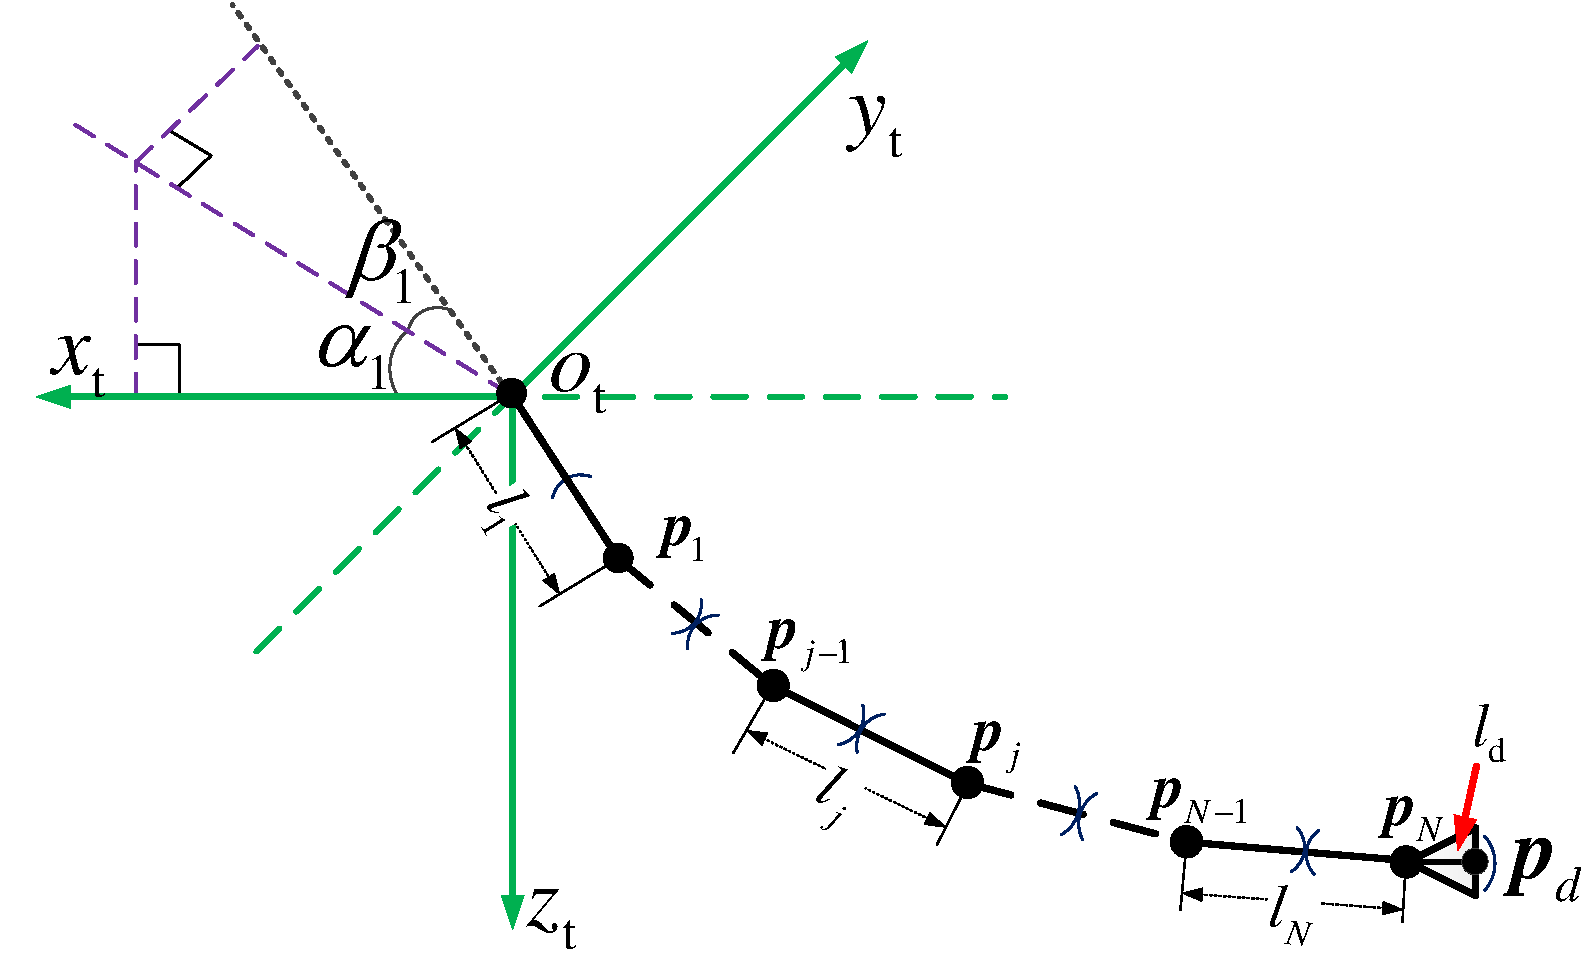
\includegraphics[width=0.5\textwidth]{Figures/Figs_Ch3/fig2.pdf}
	\caption{Link-connected hose-dogue model}\label{fig4.2}
\end{figure}

\subsection{Kinematic Equations}
The link-connected model is established in the tanker coordinate system. Since the rotation of the link around itself is not considered, the direction of each link can be described using two angles, ${\alpha _j},{\beta _j}$, as shown in Fig. \ref{fig4.2}. For example, ${\alpha _1},{\beta _1}$ represent the direction angles of the first link. Then, the relationship between the two spherical joints can be expressed using these direction angles
\begin{equation}\label{eq4.74}
{{{\bf{p}}}_{j /{\left( {j - 1} \right)}}}=  - {l_j}{{{\bf{n}}}_j},j = 1,2, \ldots ,N
\end{equation}
where ${{{\bf{n}}}_j} \in \mathbb{R}^{3}$ represents the direction of the $j$th link and can be obtained from the following equations
\begin{equation}\label{eq4.75}
{{{\bf{n}}}_j}{\rm{ = }}\left[ {\begin{array}{*{20}{c}}
	{\cos {\alpha _j}\cos {\beta _j}}\\
	{\sin {\beta _j}}\\
	{ - \sin {\alpha _j}\cos {\beta _j}}
	\end{array}} \right] \, .
\end{equation}
According to Eq. (\ref{eq4.74}), the position relationship between each mass point can be obtained as follows
\begin{equation}\label{eq4.76}
{{{\bf{p}}}_j} = {{{\bf{p}}}_{j - 1}} + {{\bf{p}}}_{j/(j-1)} ,j = 1,2, \ldots ,N
\end{equation}
Taking the derivative of it, the kinematic relationships between each mass point can be obtained as follows
\begin{equation}\label{eq4.77}
{{{\bf{v}}}_j} = {{{\bf{v}}}_{j - 1}} + {\dot {\bf{p}}}_{j /\left( j - 1\right)} ,{{{\bf{a}}}_j} = {{{\bf{a}}}_{j - 1}} + {\ddot {\bf{p}}}_{j /\left( {j - 1} \right)} ,j = 1,2, \ldots ,N
\end{equation}
where ${\bf{v}}_{j}$ and ${\bf{a}}_{j}$  represent the velocity and acceleration of the $j$th mass point, respectively. Note that since this model is established in the tanker coordinate system, and during the docking process, the tanker coordinate system is equivalent to an inertial frame, the effects of the tanker's motion on the model is not considered in this section. If readers need to consider the influence of the tanker's motion on this model, they can refer to Ref. \cite{ro_modeling_2010}.

As described above, the fundamental variables to represent the link-connected model are the attitude angles of each link. Therefore, the kinematic model should ultimately be expressed in terms of these attitude angles. Thus, expanding Eq. (\ref{eq4.77}), one can obtain
\begin{equation}\label{eq4.78}
{{\dot {\bf{p}}}_{j /\left( {j - 1} \right)}}  =  - {\dot l_j}{{{\bf{n}}}_j} - {l_j}{{\dot {\bf{n}}}_j} =  - {\dot l_j}{{{\bf{n}}}_j} - {l_j}\left( {\frac{{\partial {{{\bf{n}}}_j}}}{{\partial {\alpha _j}}}{{\dot \alpha }_j} + \frac{{\partial {{{\bf{n}}}_j}}}{{\partial {\beta _j}}}{{\dot \beta }_i}} \right)
\end{equation}
\begin{equation}\label{eq4.79}
{{\ddot {\bf{p}}}_{{j/\left( {j - 1} \right)}}} =  - {\ddot l_j}{{{\bf{n}}}_j} - 2{\dot l_j}{{\dot {\bf{n}}}_j} - {l_j}\left( {\frac{{\partial {{{\dot {\bf{n}}}}_j}}}{{\partial {\alpha _j}}}{{\dot \alpha }_j} + \frac{{\partial {{{\dot {\bf{n}}}}_j}}}{{\partial {\beta _j}}}{{\dot \beta }_i}{\rm{ + }}\frac{{\partial {{{\bf{n}}}_j}}}{{\partial {\alpha _j}}}{{\ddot \alpha }_j} + \frac{{\partial {{{\bf{n}}}_j}}}{{\partial {\beta _j}}}{{\ddot \beta }_i}} \right)
\end{equation}
Since ${\bf{n}}_{j}$ represents a direction vector, then
\begin{equation}\label{eq4.80}
\frac{{\partial {{\bf{n}}}_j^\mathrm{T}}}{{\partial {\alpha _j}}} \cdot \frac{{\partial {{{\bf{n}}}_j}}}{{\partial {\beta _j}}} = \frac{{\partial {{\bf{n}}}_j^\mathrm{T}}}{{\partial {\alpha _j}}} \cdot {{{\bf{n}}}_j} = \frac{{\partial {{\bf{n}}}_j^\mathrm{T}}}{{\partial {\beta _j}}} \cdot {{{\bf{n}}}_j} = {\dot {\bf{n}}}_j^\mathrm{T} \cdot {{{\bf{n}}}_j} = 0,\left\| {{{{\bf{n}}}_j}} \right\| = \left\| {{{{\dot {\bf{n}}}}_j}} \right\| = 1
\end{equation}
From Eqs. (\ref{eq4.75}), (\ref{eq4.78}), (\ref{eq4.79}), and (\ref{eq4.80}), one can obtain
\begin{equation}\label{eq4.81}
\left\{ \begin{array}{c}
{{\ddot \alpha }_j} = \frac{1}{{{l_j}}}\frac{{\partial { {{\bf{n}}}_j}}}{{\partial {\alpha _j}}}\left( { - \left( {{ {{\bm{a}}}_j} - { {{\bm{a}}}_{j - 1}}} \right) - 2{{\dot l}_j}{{ {\dot {\bf{n}}}}_j} - {l_j}\left( {\frac{{\partial {{ {\dot {\bf{n}}}}_j}}}{{\partial {\alpha _j}}}{{\dot \alpha }_j} + \frac{{\partial {{ {\dot {\bf{n}}}}_j}}}{{\partial {\beta _j}}}{{\dot \beta }_j}} \right)} \right)\\
{{\ddot \beta }_j} = \frac{1}{{{l_j}}}\frac{{\partial { {{\bf{n}}}_j}}}{{\partial {\beta _j}}}\left( { - \left( {{ {{\bm{a}}}_j} - { {{\bm{a}}}_{j - 1}}} \right) - 2{{\dot l}_j}{{ {\dot {\bf{n}}}}_j} - {l_j}\left( {\frac{{\partial {{ {\dot {\bf{n}}}}_j}}}{{\partial {\alpha _j}}}{{\dot \alpha }_j} + \frac{{\partial {{ {\dot {\bf{n}}}}_j}}}{{\partial {\beta _j}}}{{\dot \beta }_j}} \right)} \right)
\end{array} \right.
\end{equation}
which represents the kinematic equations of the link-connected model.

\subsection{Dynamic Equations}

Air flows over the $j$th link creat frictional drag ${{{\bf{D}}}_{{\rm{F}},j}} \in \mathbb{R}^3$ along the link direction and pressure difference drag ${{{\bf{D}}}_{{\rm{D}},j}} \in \mathbb{R}^3$ perpendicular to the cylinder's direction. The combination of these forces gives the aerodynamic force ${{{\bf{D}}}_{j}} \in \mathbb{R}^3$ acting on the cylinder. For the link-connected model, the dynamic force acting on each link needs to be distributed equally to its two end mass points, so each mass point is subjected to five forces. Define the airspeed of the tanker and eack link as follows
\begin{equation}\label{eq4.82}
{{\bf{v}}}_{{\rm{t/w}}}^{\rm{g}} =  {{\bf{v}}}_{\rm{t}}^{\rm{g}} -  {{\bf{v}}}_{\rm{w}}^{\rm{g}}, {{\bf{v}}}_{j{\rm{/w}}}^{\rm{g}} =  {{\bf{v}}}_{j}^{\rm{g}} -  {{\bf{v}}}_{\rm{w}}^{\rm{g}}
\end{equation}
Among them, ${{\bf{v}}}_{\rm{w}}^{\rm{g}}$ is the local wind speed. As shown in Fig. \ref{fig4.3}, these five forces are the gravity ${{{\bf{G}}}_{j}} \in \mathbb{R}^3$ acting on the mass point, the tension forces ${\mathbf{t}_{j}} \in \mathbb{R}^3,{\mathbf{t}_{j+1}} \in \mathbb{R}^3$ in the two link connectors, and the equivalent forces ${\bf{D}}_{j}/2,{\bf{D}}_{j+1}/2$ due to the aerodynamic forces acting on the two links at that point. For the last mass point $m_{N}$, since the next link is replaced by a drogue, its force situation is different, as shown in Fig. \ref{fig4.4}. The five forces acting on $m_{N}$ are the tension force $t_{N}$ in the $N$th link and its equivalent aerodynamic force ${\bf{D}}_{N}/2$, the gravity of the mass point and the drogue ${{{\bf{G}}}_{N}} \in \mathbb{R}^3,{{{\bf{G}}}_\text{d}} \in \mathbb{R}^3$, and the aerodynamic force ${{{\bf{G}}}_\text{d}} \in \mathbb{R}^3$ acting on the drogue.
\begin{figure}[th]
	\centering
	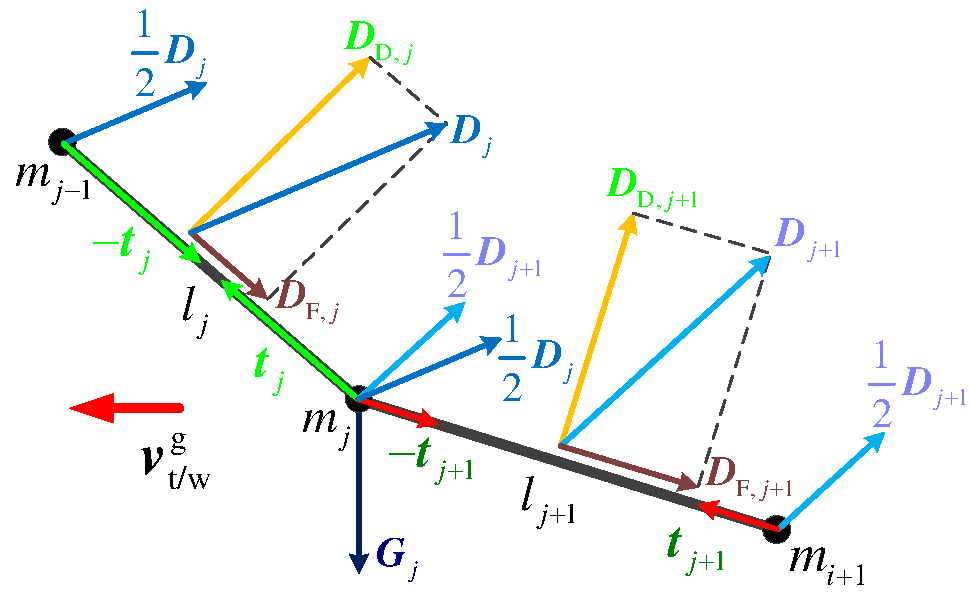
\includegraphics[width=0.5\textwidth]{Figures/Figs_Ch3/fig3.pdf}
	\caption{Analysis of forces on the first $N-1$ links}\label{fig4.3}
\end{figure}
\begin{figure}[th]
	\centering
	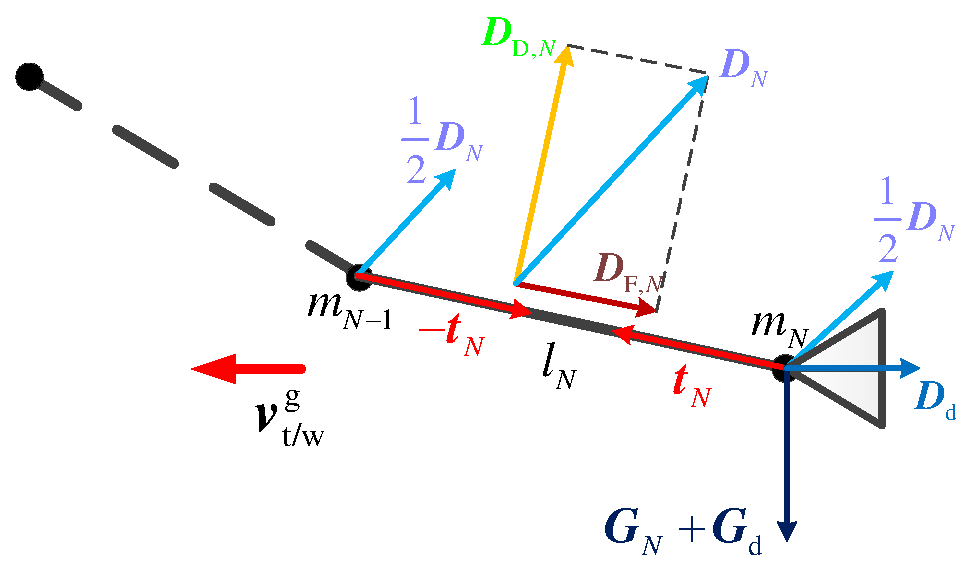
\includegraphics[width=0.5\textwidth]{Figures/Figs_Ch3/fig4.pdf}
	\caption{Analysis of forces on the $N$th link}\label{fig4.4}
\end{figure}

According to aerodynamics principles, the calculation of friction drag and pressure drag is as follows
\begin{equation}\label{eq4.83}
{ {{\bf{D}}}_{{\rm{F}},j}} =  - \left[ {{{\rm{C}}_{{\rm{F}},j}}{\rho _\infty }{{\left( { {{\bf{v}}}_{j{\rm{/w}}}^{\rm{g}} \cdot { \mathbf{n}_{{\rm{F}},j}}} \right)}^2}\left( {\pi {r_j}{l_j}} \right)} \right]{ \mathbf{n}_{{\rm{F}},j}}
\end{equation}
\begin{equation}\label{eq4.84}
{ {{\bf{D}}}_{{\rm{D}},j}} =  - \left[ {{{\rm{C}}_{{\rm{D}},j}}{\rho _\infty }{{\left( {{\mathbf{n}_{{\rm{D}},j}} \cdot {\mathbf {n}_{{\rm{D}},j}}} \right)}^2}\left( {\pi {r_j}{l_j}} \right)} \right]{\mathbf {n}_{{\rm{D}},j}}
\end{equation}
where ${\rho _\infty }$ represents the density of the stationary air at that altitude, and ${\mathbf {n}_{{\rm{F}},j}},{\mathbf {n}_{{\rm{D}},j}}$ are the directions of the two forces, which can be expressed as
\begin{equation}\label{eq4.85}
{\mathbf {n}_{{\rm{F}},j}} = {\mathbf {n}_j},{\mathbf {n}_{{\rm{D}},j}} =  {{\mathbf{v}}}_{j{\rm{/w}}}^{\rm{g}} - \left( { {{\mathbf{v}}}_{j{\rm{/w}}}^{\rm{g}} \cdot {\mathbf {n}_j}} \right){\mathbf {n}_j}
\end{equation}
The parameters ${{\rm{C}}_{{\rm{F}},j}}$ and ${{\rm{C}}_{{\rm{D}},j}}$ represent aerodynamic coefficients. According to Ref. \cite{vassberg_numerical_2003}, before calculating ${{\rm{C}}_{{\rm{F}},j}}$ and ${{\rm{C}}_{{\rm{D}},j}}$, it is necessary to compute the Reynolds number of the fluid at each link's location.
\begin{equation}\label{eq4.86}
{{\mathop{\rm Re}\nolimits} _j} = \frac{{{\rho _j}\left\| { {{\mathbf{v}}}_{j{\rm{/w}}}^{\rm{g}}} \right\|{l_{{\rm{ch}},j}}}}{\upsilon } \approx \frac{{{\rho _\infty }\left\| { {{\mathbf{v}}}_{j/{\rm{w}}}^{\rm{g}}} \right\|{l_{{\rm{ch}},j}}}}{\upsilon }
\end{equation}
where ${\rho _\infty }$ is the local fluid density, and since the airflow compression during the docking process can be neglected, it is approximately equivalent to the density of static atmosphere at that altitude. $\upsilon $ is the dynamic viscosity coefficient of the local atmosphere, and ${l_{{\rm{ch}},j}}$ is the characteristic length of the $j$th link, represented as
\begin{equation}\label{eq4.87}
{l_{{\rm{ch}},j}} = \frac{{\pi {r_{\rm{h}}}}}{{\sin {\vartheta _j}}}
\end{equation}
where ${\vartheta _j}$ is the angle between the link and the airspeed $ {{\mathbf{v}}}_{j{\rm{/w}}}^{\rm{g}}$, and ${r_{\rm{h}}}$ is the outer radius of the hose, i.e.
\begin{equation}\label{eq4.88}
{\vartheta _j} = \arccos \frac{{{\mathbf {n}_j^\mathrm{T}}   {{\mathbf{v}}}_{j{\rm{/w}}}^{\rm{g}}}}{{\left\| {{\mathbf {n}_j}} \right\|\left\| { {{\mathbf{v}}}_{j{\rm{/w}}}^{\rm{g}}} \right\|}} \, .
\end{equation}
After obtaining the Reynolds number, ${{\rm{C}}_{{\rm{F}},j}}$ and ${{\rm{C}}_{{\rm{D}},j}}$ can be determined based on the Reynolds number, as shown in Table \ref{tab4.1}.
\begin{table}[th]
	\caption{The relations among ${{\rm{C}}_{{\rm{F}},j}},{{\rm{C}}_{{\rm{D}},j}}$ and ${{\mathop{\rm Re}\nolimits} _j}$}
	\renewcommand\arraystretch{1.3}
	\centering
	\begin{tabular}	
		[c]{|c|c|c|c|}
		
		\hline
		${{\mathop{\rm Re}\nolimits} _j}$ &${{\rm{C}}_{{\rm{F}},j}}$&${{\mathop{\rm Re}\nolimits} _j}$&${{\rm{C}}_{{\rm{D}},j}}$
		\\\hline
		$\left( {{{10}^{ - 2}},{{10}^4}} \right]$&$4.6409{{\mathop{\rm Re}\nolimits} ^{ - 0.6667}}$&$\left( {{{10}^{ - 2}},1} \right]$&$10{{\mathop{\rm Re}\nolimits} ^{ - 0.81}}$
		\\\hline
		$\left( {{{10}^4},{{10}^{10}}} \right]$ &$0.0464{{\mathop{\rm Re}\nolimits} ^{ - 0.1667}}$&$\left( {1,180} \right]$&$10{{\mathop{\rm Re}\nolimits} ^{ - 0.4083}}$
		\\\hline
		$\left( {{{10}^{10}}, + \infty } \right]$&$0.001$&$\left( {180,4 \times {{10}^5}} \right]$&$1.2$
		\\\hline
		& &$\left( {4 \times {{10}^5},4 \times {{10}^6}} \right]$&$0.002128{{\mathop{\rm Re}\nolimits} ^{ - 0.3522}}$
		\\\hline
		& &$\left( {4 \times {{10}^6}, + \infty } \right]$&$0.45$
		\\\hline
	\end{tabular}
	\label{tab4.1}
\end{table}
Additionally, the drogue also experiences aerodynamic forces. Ref. \cite{ro_aerodynamic_2007} analyzed the aerodynamic forces acting on the drogue and provided the equation for the aerodynamic force on the drogue as follows
\begin{equation}\label{eq4.89}
{ {{\bf{D}}}_{\rm{d}}} = \frac{1}{2}{{\rm{C}}_{\rm{d}}}{\rho _\infty }\left( { {({\mathbf{v}}}_{N{\rm{/w}}}^{\rm{g}})^\mathrm{T}  {{\mathbf{v}}}_{N{\rm{/w}}}^{\rm{g}}} \right)\left( {\pi {r_{\rm{d}}}} \right)\left( {\frac{{ {{\mathbf{v}}}_{N{\rm{/w}}}^{\rm{g}}}}{{\left\| { {{\mathbf{v}}}_{N{\rm{/w}}}^{\rm{g}}} \right\|}}} \right)
\end{equation}
where ${r_{\rm{d}}}$ is the radius of the drogue canopy, and ${{\rm{C}}_{\rm{d}}}$ is a coefficient determined by the drogue strut angle as shown in Fig. \ref{fig4.5} and the canopy area, and so on. Typically, this coefficient is taken as 0.8 \cite{ro_aerodynamic_2007}. At this point, all forces except for the tension are known. The following section provides the method for calculating the tension.
\begin{figure}[th]
	\centering
	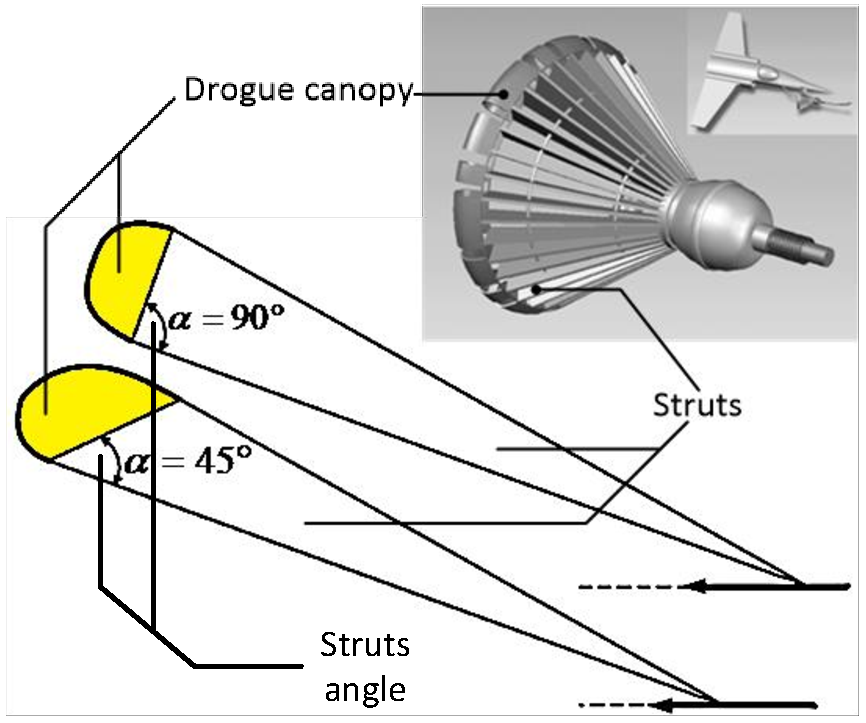
\includegraphics[width=0.5\textwidth]{Figures/Figs_Ch3/fig5.pdf}
	\caption{Drogue canopy's angle of struts}\label{fig4.5}
\end{figure}

\subsection{Calculation of Tension}
In the link-connected model, since the tension force is generated internally within the system, it is considered an internal force, while the other forces are external forces. For ease of calculation, the external forces composed of aerodynamic forces and gravity are denoted as ${{{\bf{Q}}}_j} \in\mathbb{R}^{3} $, i.e,
\begin{equation}\label{eq4.90}
\left\{ \begin{array}{l}
{ {{\bf{Q}}}_j} = {m_j}\bm{g} + \frac{1}{2}\left( {{ {{\bf{D}}}_j} + { {{\bf{D}}}_{j + 1}}} \right),j = 1,2, \ldots ,N - 1\\
{ {{\bf{Q}}}_N} = \left( {{m_N} + {m_{\rm{d}}}} \right) {\bm{g} + }\frac{1}{2}{ {{\bf{D}}}_N} + { {{\bf{D}}}_{\rm{d}}} + {\mathbf{F}_{\rm{b}}}\, .
\end{array} \right.
\end{equation}
Assume the tension at the two ends of the same link is ${t_j}{ {{\mathbf{n}}}_j}$ and $ - {t_j}{ {{\mathbf{n}}}_j}$, where ${t_j}$ is a constant, which satisfies the property that the tension at both ends of the link has the same magnitude, opposite direction, and along the link. Here, ${\mathbf{F}_{\rm{b}}}$ represents other external disturbances acting on the drogue, and it actually includes the bow wave, which is included in the external forces acting on the last mass point. Therefore, according to Newton's second law, one has
\begin{equation}\label{eq4.91}
\left\{ \begin{array}{l}
{ {{\bf{a}}}_j} = \frac{{{t_j}{ {{\mathbf{n}}}_j} - {t_{j + 1}}{ {{\mathbf{n}}}_{j + 1}} + { {{\bf{Q}}}_j}}}{{{m_j}}},j = 1,2, \ldots ,N - 1\\
{ {{\bf{a}}}_N} = \frac{{{t_N}{ {{\mathbf{n}}}_N} + { {{\bm{Q}}}_N}}}{{{m_N}}}
\end{array} \right.
\end{equation}
where ${ {{\bf{a}}}_j}$ represents the acceleration of the $j$th link, and ${ {{\bf{a}}}_N}$ represents the acceleration of the drogue.

On the other hand, since
\begin{equation}\label{eq4.92}
\mathbf{p}_{{j/ {\left( {j - 1} \right)}}}^\mathrm{T} \cdot {\mathbf {p}_{{j /{\left( {j - 1} \right)}}}} = l_j^2
\end{equation}
Taking the second derivative of both sides of this equation, it can be obtained
\begin{equation}\label{eq4.93}
{{\mathbf{n}}}_j^\mathrm{T} \cdot \left( {{ {{\bf{a}}}_j} - { {{\bf{a}}}_{j - 1}}} \right) = {l_j} {\dot {\mathbf{n}}}_j^\mathrm{T}{ {\dot {\mathbf{n}}}_j} - {\ddot l_j}
\end{equation}
Therefore, by combining Eq. (\ref{eq4.91}) and Eq. (\ref{eq4.93}) and rearranging them
\begin{equation}\label{eq4.94}
{\bf{T}}^\mathrm{T}   {\bf{t} = \bm{q}}
\end{equation}
where $ {\bf{t} = }{\left[ {\begin{array}{*{20}{c}}
		{{t_1}}&{{t_2}}& \cdots &{{t_N}}
		\end{array}} \right]^{\rm{T}}}$, and the coefficient matrix ${\bf{T}}$ is known in terms of $\bm{q}$ (its specific form will be described in the next section). With this, the relationship between internal force and external force can be established. By solving Eq. (\ref{eq4.91}), we can obtain ${\bm{a}}_{j}$ and then update it in Eq. (\ref{eq4.81}). This completes the entire link-connected model.

The block diagram of the link-connected hose-drogue model can be obtained based on the above steps, as shown in the Fig. \ref{fig4.6}.
\begin{figure}[th]
	\centering
	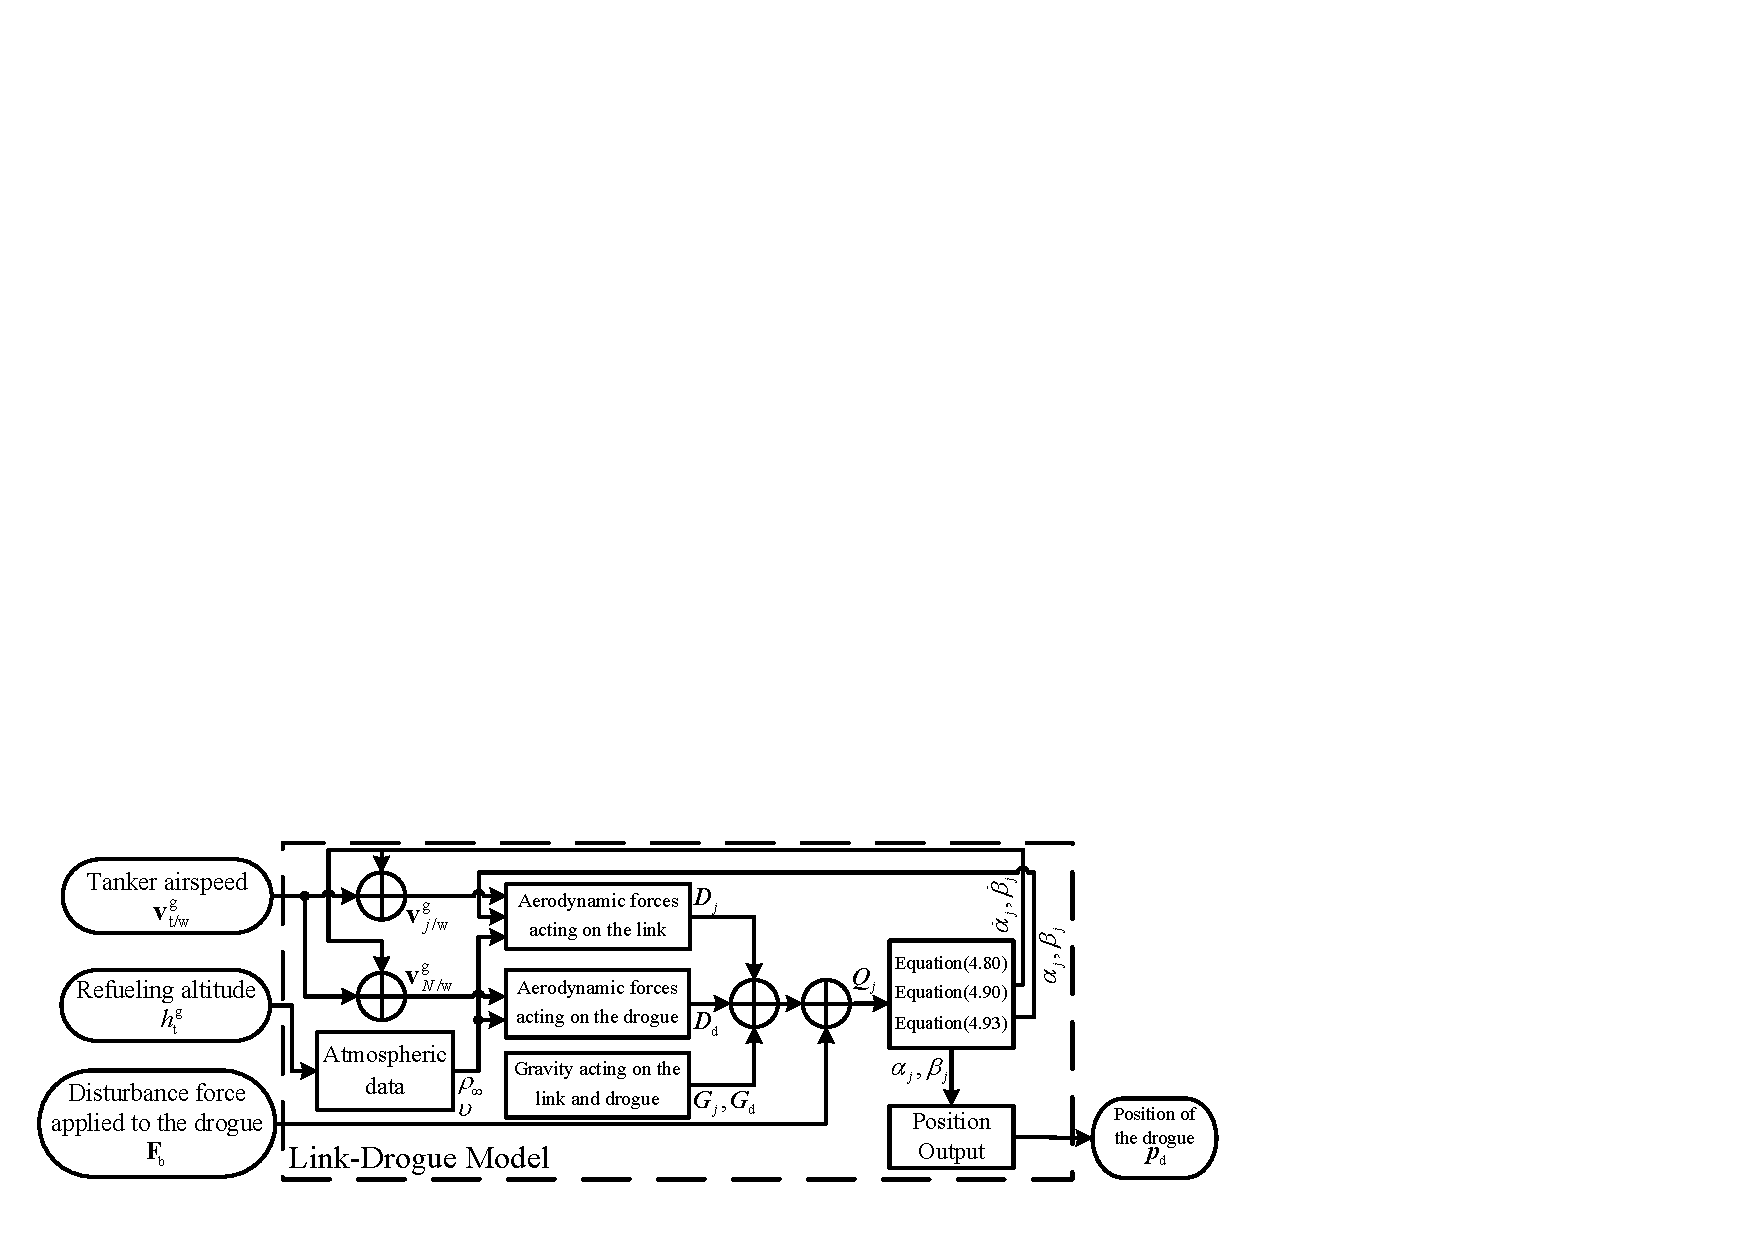
\includegraphics[width=0.9\textwidth]{Figures/Figs_Ch3/fig6.pdf}
	\caption{Flowchart of the link-connected hose-drogue model calculation}\label{fig4.6}
\end{figure}

\subsection{Link-connected Model during Hose Contraction}
It should be noted that due to the presence of the Hose Drum Unit (HDU) in the system, the hose-drogue may retract a certain distance into the refueling pod when subjected to strong disturbances. For the subsequent modeling needs, it is necessary to consider the retraction of the link. If the retraction distance of the link is less than the length of the first link, we will consider the equation for the tension of $N$ links. However, if the disturbances are significant and the retraction length exceeds the length of the first link, the order of the equation will change. Assume that the link visible outside the HDU is the original $i$th link, then Eq. (\ref{eq4.94}) satisfies the following form
\begin{equation}\label{eq4.95}
\left[ {\begin{array}{*{20}{c}}
	{{{\bf{0}}_{\left( {i - 1} \right) \times \left( {i - 1} \right)}}}&{\bf{0}}\\
	{\bf{0}}&{{{{\bf{\bar T}}}_{\left( {N - i + 1} \right) \times \left( {N - i + 1} \right)}}}
	\end{array}} \right] {\bf{t} = }\left[ {\begin{array}{*{20}{c}}
	{{{\bf{0}}_{\left( {i - 1} \right) \times 1}}}\\
	{{{ {\bar {\bm{q}}}}_{\left( {N - i + 1} \right) \times 1}}}
	\end{array}} \right]
\end{equation}
where ${\bf{\bar{ T}}}$ and ${\bar{\bm{q}}}$ are as follows
%where ${\bf{\bar {T}}}$ and $ {\bar {\bm{q}}}$ are as follows:
\begin{equation}\label{eq4.96}
{\bf{\bar T}} = \left[ {\begin{array}{*{20}{c}}
	1&{ - { {{\bf{n}}}^\mathrm{T}_i}{ {{\bf{n}}}_{i{\rm{ + }}1}}}&0& \cdots & \cdots \\
	{ - {\mu _i}{ {{\bf{n}}}^\mathrm{T}_i}{ {{\bf{n}}}_{i + 1}}}&{{\mu _i} + {\mu _{i + 1}}}&{ - {\mu _{i + 1}}{ {{\bf{n}}}^\mathrm{T}_{i + 1}}{ {{\bf{n}}}_{i{\bf{ + }}2}}}&0& \cdots \\
	0& \ddots &0& \cdots & \cdots \\
	0&{ - {\mu _{j - 1}}{ {{\bf{n}}}^\mathrm{T}_{j - 1}}{ {{\bf{n}}}_j}}&{{\mu _{j - 1}} + {\mu _j}}&{{\mu _j}{ {{\bf{n}}}^\mathrm{T}_j}{ {{\bf{n}}}_{j + 1}}}&0\\
	0& \cdots & \ddots &0& \cdots \\
	0&0&{ - {\mu _{N - 2}}{ {{\bf{n}}}^\mathrm{T}_{N - 2}}{ {{\bf{n}}}_{N - 1}}}&{{\mu _{N - 2}} + {\mu _{N - 1}}}&{{\mu _{N - 1}}{ {{\bf{n}}}^\mathrm{T}_{N - 1}}{ {{\bf{n}}}_N}}\\
	0& \cdots & \cdots &{ - {\mu _{N - 1}}{ {{\bf{n}}}^\mathrm{T}_{N - 1}}{ {{\bf{n}}}_N}}&{{\mu _{N - 1}} + {\mu _N}}
	\end{array}} \right]
\end{equation}
\begin{equation}\label{eq4.97}
{\bar {\bm{q}}} = \left[ {\begin{array}{*{20}{c}}
	{{m_i}{l_i}{{\dot {\mathbf{n}}}}_i^2 - {{\mathbf{Q}}^\mathrm{T}_i}{{\mathbf{n}}_i} - {m_i}{{\ddot l}_i}}\\
	{{l_{i + 1}}{\bm{\dot \mathbf {n}}}_{i + 1}^2 + \left( {{\mu _i}{{\mathbf{Q}}^\mathrm{T}_i} - {\mu _{i + 1}}{{\mathbf{Q}}^\mathrm{T}_{i + 1}}} \right){{\mathbf{n}}_{i + 1}}}\\
	\vdots \\
	{{l_j}{\bm{\dot \mathbf {n}}}_j^2 + \left( {{\mu _{j - 1}}{{\mathbf{Q}}^\mathrm{T}_{j - 1}} - {\mu _j}{{\mathbf{Q}}^\mathrm{T}_j}} \right){{\bf{n}}_j}}\\
	\vdots \\
	{{l_{N - 1}}{\bm{\dot\mathbf{n}}}_{N - 1}^2 + \left( {{\mu _{N - 2}}{{\mathbf{Q}}^\mathrm{T}_{N - 2}} - {\mu_{N - 1}}{{\mathbf{Q}}^\mathrm{T}_{N - 1}}} \right){{\mathbf{n}}_{N - 1}}}\\
	{{l_N}{\bm{\dot \mathbf {n}}}_N^2 + \left( {{\mu _{N - 1}}{{\mathbf{Q}}^\mathrm{T}_{N - 1}} - {\mu _N}{{\mathbf{Q}}^\mathrm{T}_N}} \right){{\mathbf{n}}_N}}
	\end{array}} \right]
\end{equation}
where ${\mu _j} = 1 / {{m_j}}$, and when $i = 1$, ${\bf{\bar T}} = {\bf{T}}$ and ${\bar {\bm{q}} = {\bm{q}}}$, and in this case only the first link changes.
The equation for the $i$th link being retracted exactly is 
\begin{equation}\label{eq4.98}
{t_i} - { {{\bf{n}}}^\mathrm{T}_i}{ {{\bf{n}}}_{i + 1}}{t_{i + 1}} = 0 \Rightarrow {t_i} = { {{\bf{n}}}^\mathrm{T}_i}{ {{\bf{n}}}_{i + 1}}{t_{j + 1}}
\end{equation}
This means that at this moment, the length of the link is exactly zero, the mass of the link is zero, and the aerodynamic force acting on it is also zero. On the other hand, due to the continuity of the hose, it can be assumed that its direction is aligned with the next link, and the magnitude of the tension is the same. It is seen that Eq. (\ref{eq4.98}) corresponds well to this physical process. During numerical simulations, the updating process of the calculation for the first link is illustrated by Fig. \ref{fig4.7}.
\begin{figure}[th]
	\centering
	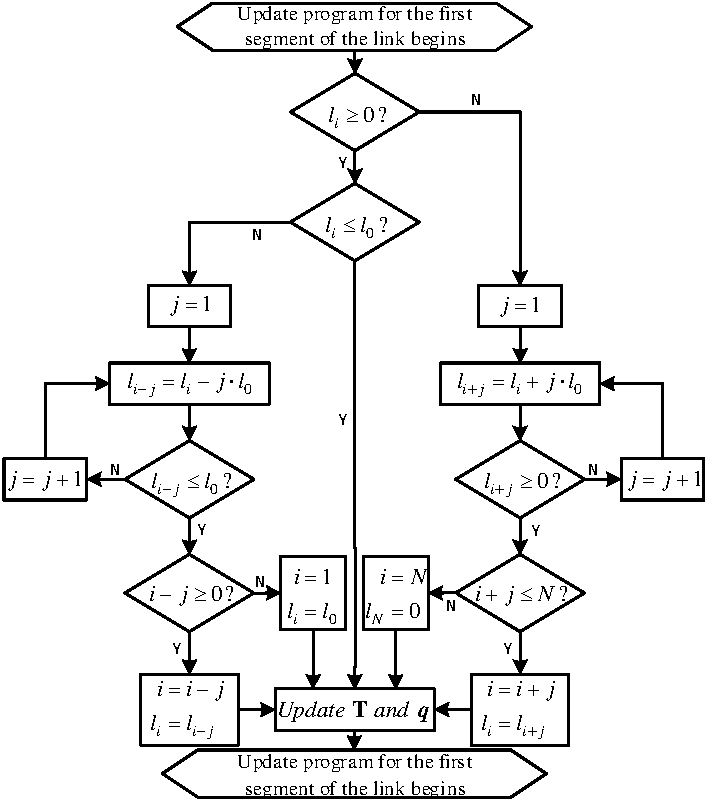
\includegraphics[width=0.7\textwidth]{Figures/Figs_Ch3/fig7.pdf}
	\caption{Updating Process of the First Link}\label{fig4.7}
\end{figure}

In the figure, ${l_0}$ represents the length of each link when it is fully extended, $j$ is the counter, and $j{l_0}$ represents the total length of $j$ links of the hose that are either retracted or extended. This process takes into account situations where the first link cannot be extended any further after being fully extended, and the last link cannot be retracted any further after being fully retracted. It also considers the possibility of encountering numerical calculation scenarios where multiple links of the hose are retracted or extended in a single step.

\subsection{Simulation Example of the link-connected hose-drogue model}

To validate the effectiveness of the link-connected model, simulations are conducted using the parameters listed in Table \ref{tab4.2}. In the table, the variable ${\rho _{\rm{h}}}$ represents the linear density of the hose, and the aerodynamic parameter ${{\rm{C}}_{\rm{d}}}$ for the drogue is typically set to 0.8. It is important to note that in this simulation, the elongation of the hose due to the Hose Drum Unit (HDU) model has not been taken into account.
\begin{table}[th]
	\caption{Simulation Parameters of the link-connected hose-drogue model}
	\renewcommand\arraystretch{1.3}
	\centering
	\begin{tabular}	
		[c]{|c|c|c|c|c|c|}
		
		\hline
		Parameters&Values&Units&Parameters&Values&Units
		\\\hline
		$ {v}_{\rm{t}}^{\rm{g}}$&${\left[ {\begin{array}{*{20}{c}}
				{120}&0&0
				\end{array}} \right]^{\rm{T}}}$&${m/s}$&${l_{\rm{d}}}$&$0.422$&$m$
		\\\hline
		$h_{\rm{t}}^{\rm{g}}$&$3000$& $m$&${l_{\rm{h}}}$&$15$&$m$
		\\\hline
		${\rho _\infty }$&$0.8443$&${{kg} /{{m^3}}}$&${r_{\rm{h}}}$&$0.034$&$m$
		\\\hline
		$\upsilon $&$1.7894 \times {10^{{\rm{ - }}5}}$&${{{m^2}} /s}$&${\rho _{\rm{h}}}$&$4.1$&${{kg} /m}$
		\\\hline
		${r_{\rm{d}}}$&$0.305$&$m$&$N$&$20$&-
		\\\hline
		${m_{\rm{d}}}$&$29.5$&$kg$&$ {w}_{\rm{t}}^{\rm{g}}$&${\left[ {\begin{array}{*{20}{c}}
				0&0&0
				\end{array}} \right]^{\rm{T}}}$&$m/s$
		\\\hline
	\end{tabular}
	\label{tab4.2}
\end{table}

(1) Simulation 1: Windless Scenario

In this simulation, the hose is allowed to fall freely from a horizontal position under no wind conditions. Specifically, when the wind velocity $ {\bf{w}}_{\rm{t}}^{\rm{g}} = {\left[ {\begin{array}{*{20}{c}}
		0&0&0
		\end{array}} \right]^{\rm{T}}}$, the hose is fully extended, and the initial conditions for each link are set to ${\alpha _j}\left( 0 \right) = {\beta _j}\left( 0 \right) = {0^ \circ },j = 1,2, \ldots ,N$. The model is then allowed to move freely, and the trajectories of the links and the drogue are observed. The simulation results are depicted in Fig. \ref{fig4.8}. Since there is no crosswind in this simulation, the position in the ${y_{\rm{t}}}$-direction remains unchanged. Observing the dynamic process, the model reaches a steady state around 20 seconds. Therefore, a moment beyond 20 seconds can be chosen as the equilibrium point of the model under the environmental conditions specified in Table \ref{tab4.2}.

(2) Simulation 2: Drogue Located at Equilibrium Position

In this simulation, the hose is initially at its equilibrium position, and a lateral perturbation is applied to the drogue at 10 seconds. Specifically, the stable state obtained from Simulation 1 is used as the initial condition for Simulation 2. At 10 seconds, a step disturbance is introduced to the system by setting the force ${{\bf{F}}_{\rm{b}}}$ to increase from ${\left[ {\begin{array}{*{20}{c}}
		0&0&0
		\end{array}} \right]^{\rm{T}}}$ to ${\left[ {\begin{array}{*{20}{c}}
		0&{50}&0
		\end{array}} \right]^{\rm{T}}}$ (Unit is N) . The trajectories of the links and the drogue under this scenario are observed. Fig. \ref{fig4.9} illustrates the trajectory of the drogue in this scenario.

From Fig. \ref{fig4.9} (d), it can be observed that under the crosswind perturbation, the drogue first swings in the direction of the wind and upwards. Subsequently, it oscillates back, forming a spiral motion, and finally stabilizes at a new equilibrium position. Moreover, Figs. \ref{fig4.9} (a)-(c) show that the dynamics of the drogue in various directions resemble those of a second-order or even higher-order linear system. This observation serves as the foundation for simplifying the model in subsequent chapters.
\begin{figure}[th]
	\centering
	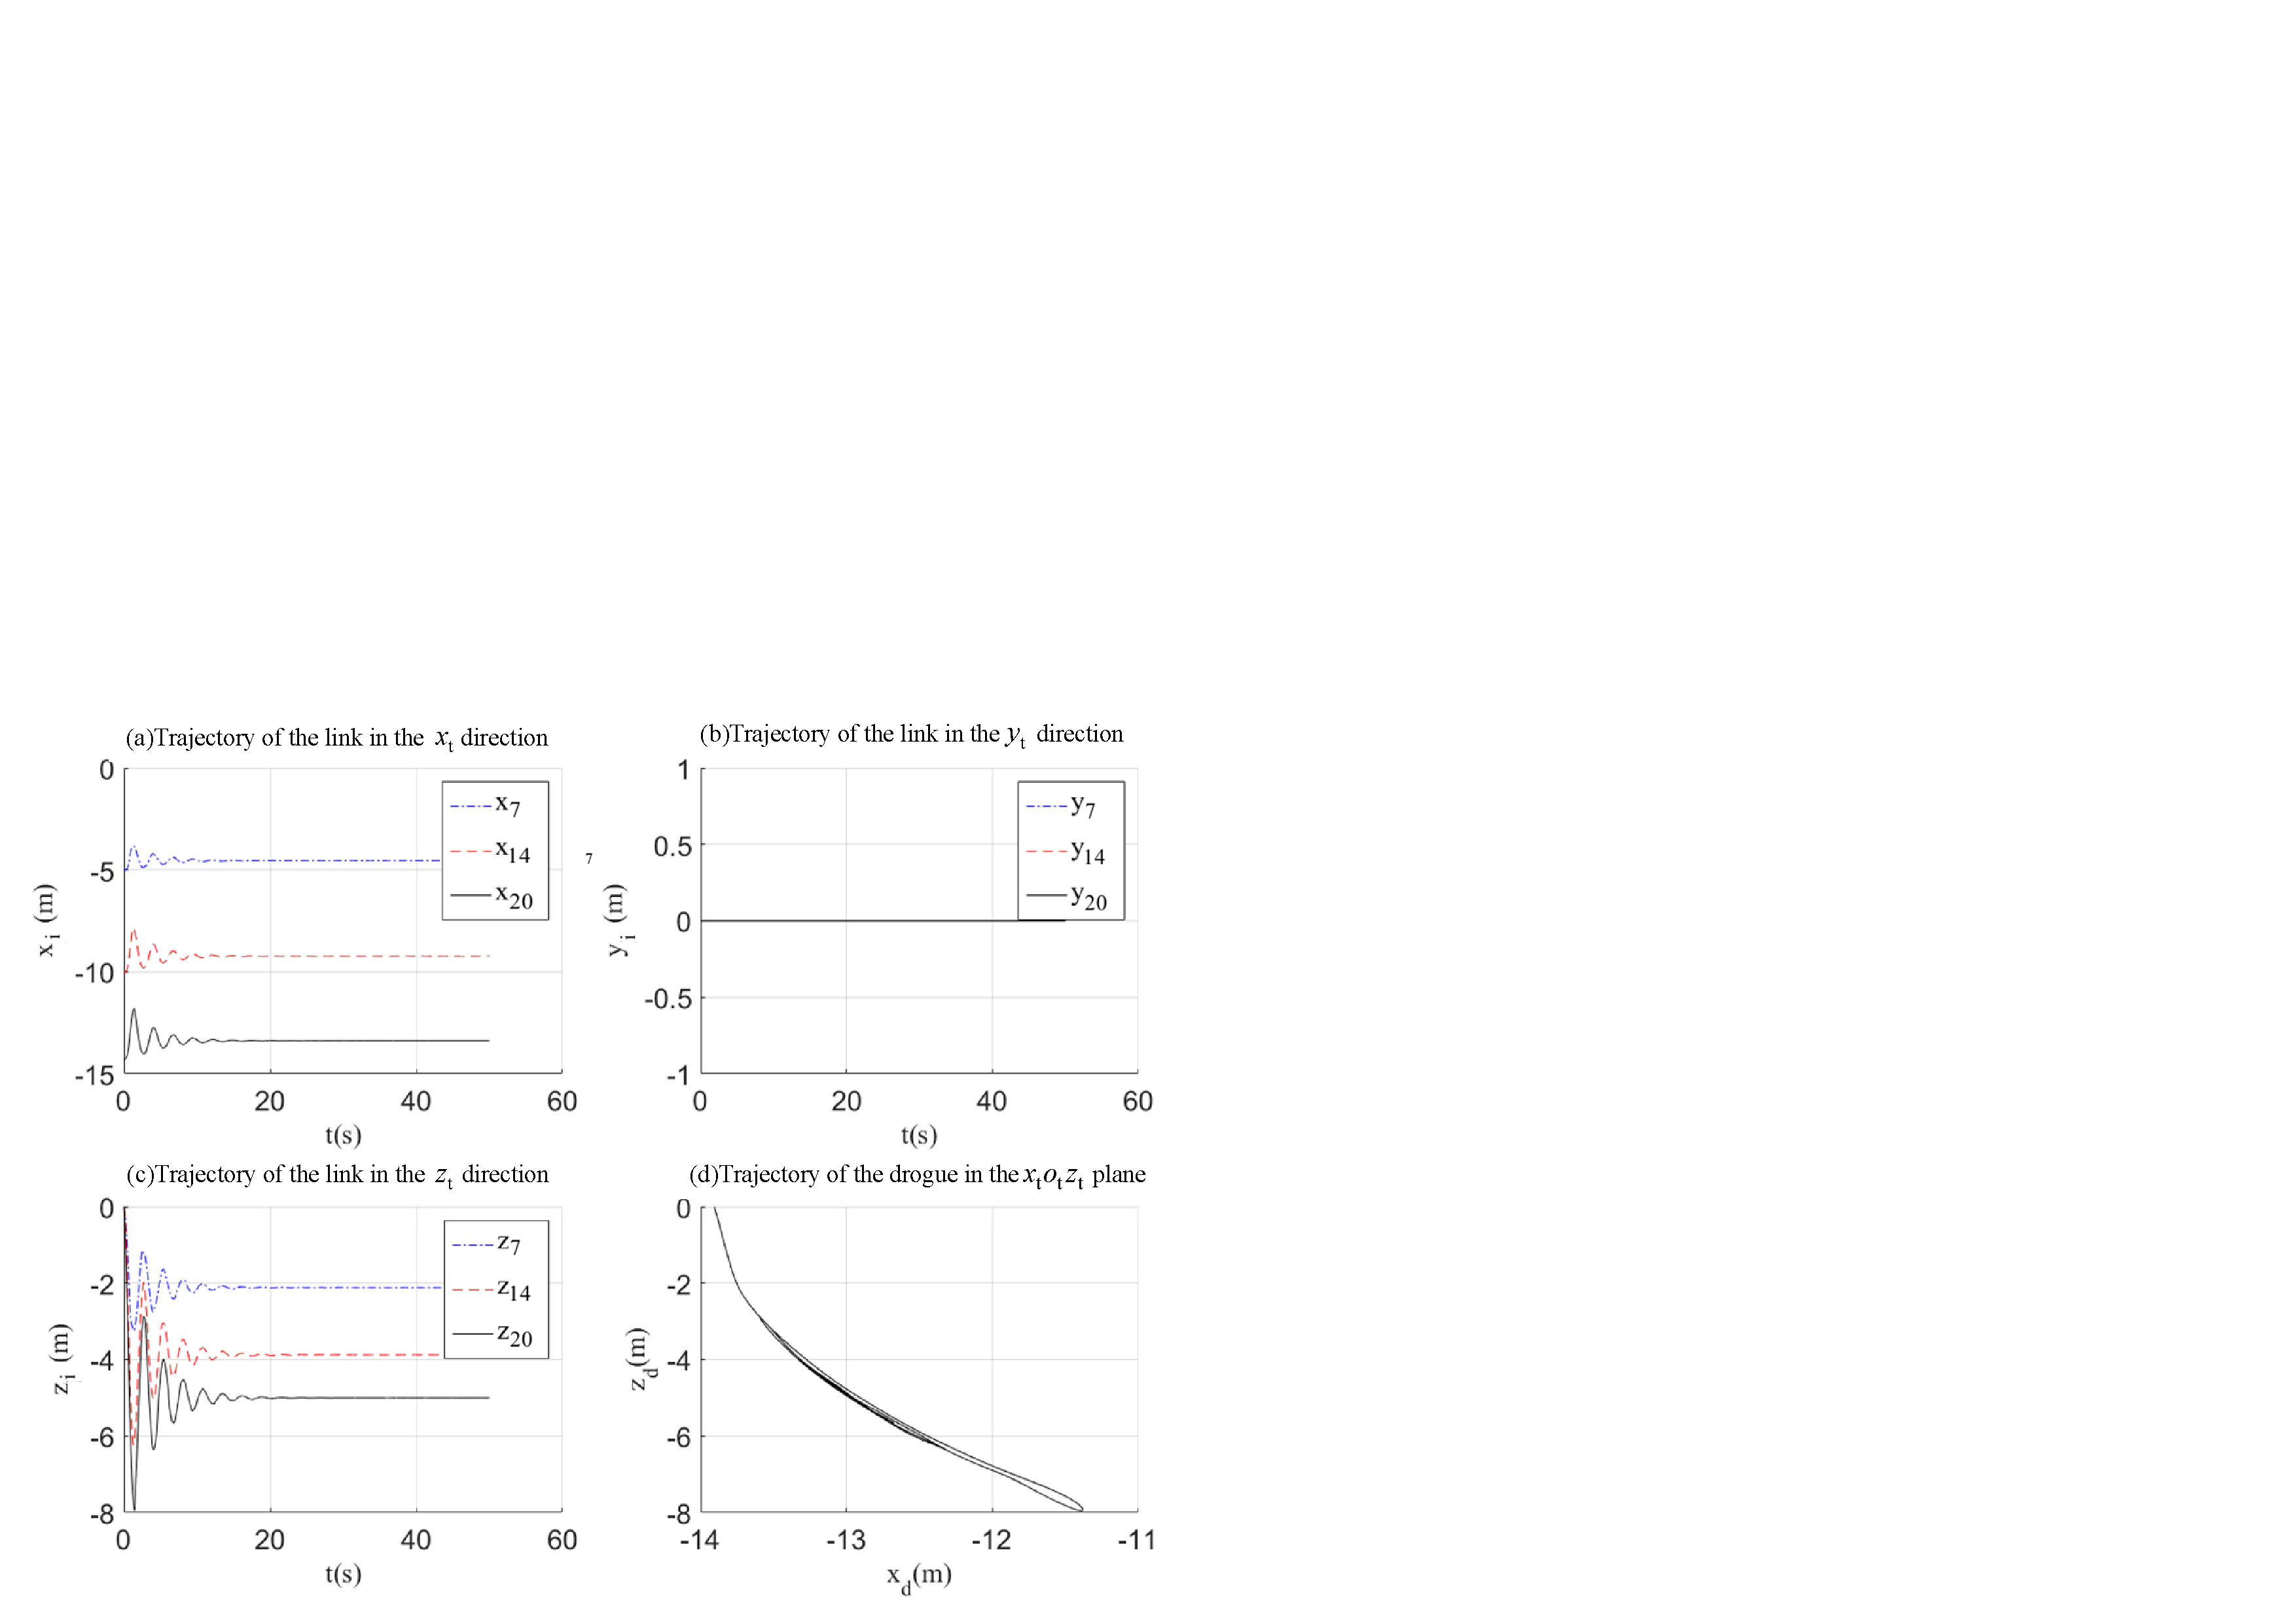
\includegraphics[width=0.8\textwidth]{Figures/Figs_Ch3/fig8.pdf}
	\caption{Simulation 1: Trajectory of the Hose in Free Fall without Wind}\label{fig4.8}
\end{figure}
\begin{figure}[th]
	\centering
	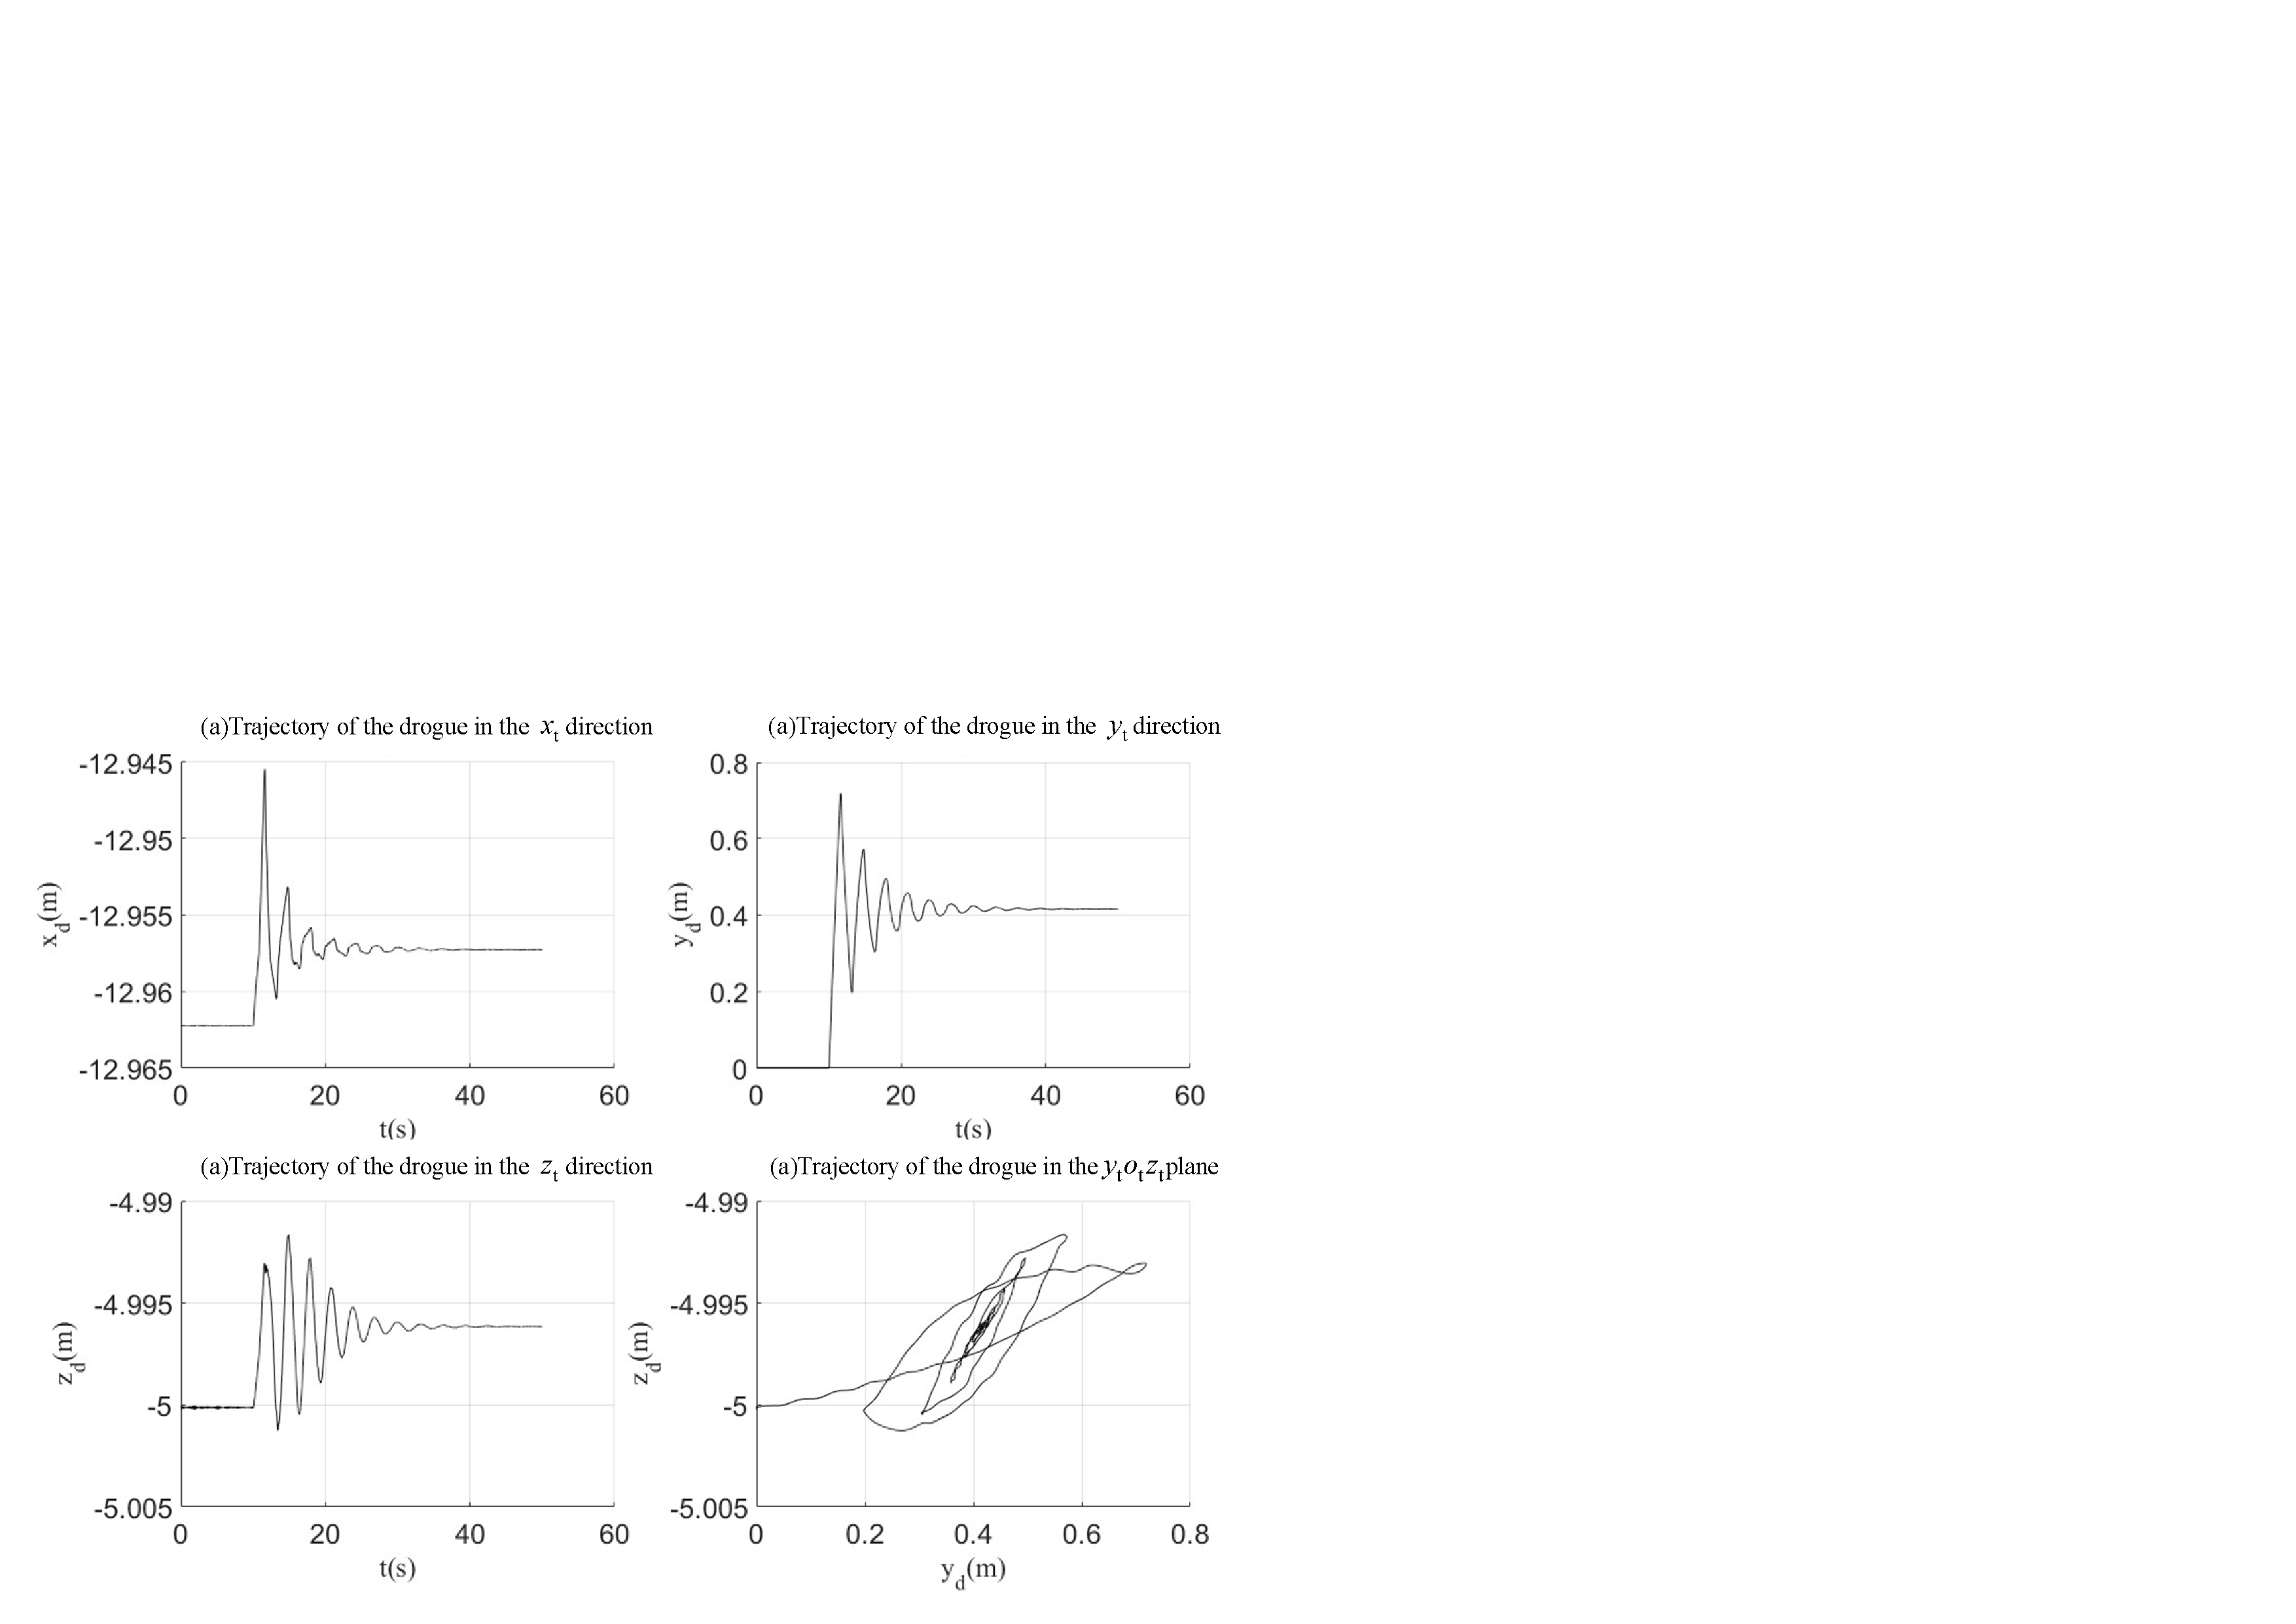
\includegraphics[width=0.8\textwidth]{Figures/Figs_Ch3/fig9.pdf}
	\caption{Simulation 2: Trajectory of the Drogue Under Crosswind Conditions}\label{fig4.9}
\end{figure}

%\section{Drogue Dynamic Model with HDU}
%In the probe-and-drogue refueling system, a device is installed at the front end of the hose to release or withdraw the hose, known as the Hose Drum Unit (HDU), also referred to as the Reel Take-Up System. This unit is situated within the refueling pod, as shown in Fig. \ref{fig4.22}. The HDU primarily consists of a drum (reel) that winds the hose, a motor responsible for controlling the rotation of the drum, and a controller for the motor. The rotation of the motor is primarily controlled based on the status of the upper end of the hose connected to the refueling pod. This device regulates the hose tension by adjusting the length of the hose exposed outside when the hose tension is insufficient. It effectively mitigates the phenomenon of hose whipping by reducing the risk of sudden tension changes, thereby minimizing potential refueling accidents caused by such effects.
%\begin{figure}[th]
%	\centering
%	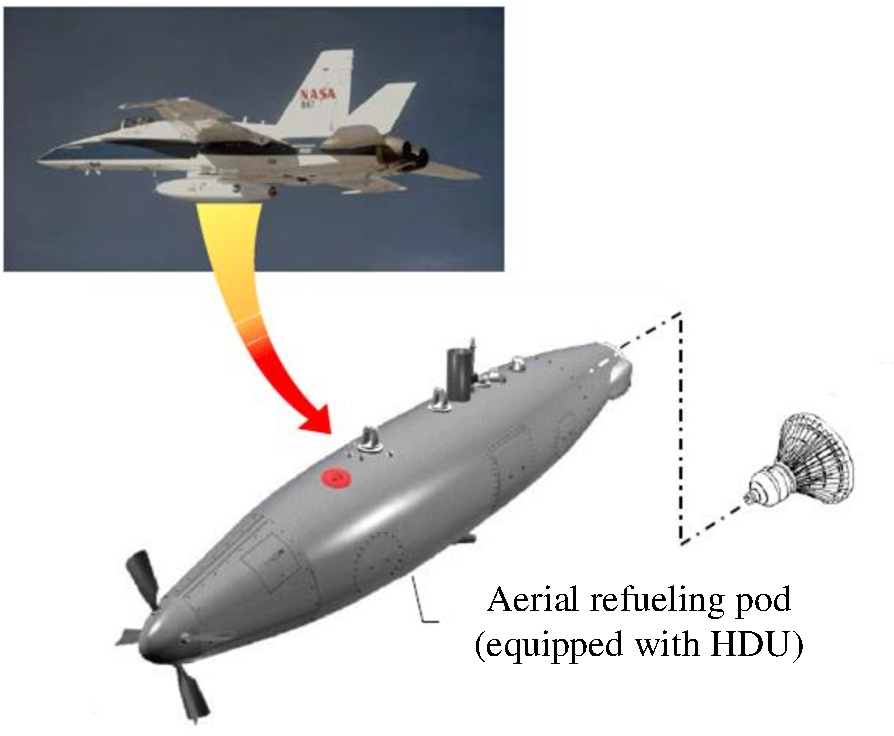
\includegraphics[width=0.6\textwidth]{Chap4/fig22.pdf}
%	\caption{Refueling Pod and HDU Schematic}\label{fig4.22}
%\end{figure}
%Currently, research on the HDU primarily focuses on designing controllers to regulate the hose tension and suppress hose whipping phenomenon. Hose whipping usually occurs after the docking of the drogue and probe, but the HDU's role in suppressing hose whipping also affects the dynamics of the hose-drogue assembly during the docking process. However, this aspect has received relatively little attention in current research. Therefore, this section will provide an initial analysis of this impact.
%
%\subsection{Analysis of Fixed-Length link-connected model Deficiencies}
%
%Based on the analysis in Section 4.3.4, the significant downward movement of the drogue in the ${o_{\rm{t}}}{z_{\rm{t}}}$ direction compared to the experiment can be observed. From this phenomenon and the corresponding time of occurrence, it can be inferred that this dynamic motion of the drogue in the ${o_{\rm{t}}}{z_{\rm{t}}}$ direction is caused by the component of the bow wave in the ${o_{\rm{t}}}{x_{\rm{t}}}$ direction, meaning that the force in the ${o_{\rm{t}}}{x_{\rm{t}}}$ direction induces a substantial displacement of the drogue in the ${o_{\rm{t}}}{z_{\rm{t}}}$ direction. The reason behind this phenomenon is that the hose-drogue system is under tension when in a steady state, making the hose behave more rigidly. The hose-drogue system is approximately similar to a simple pendulum near its equilibrium position \cite{williamson_controllable_2010}, as depicted in Fig. \ref{fig4.23}.
%\begin{figure}[th]
%	\centering
%	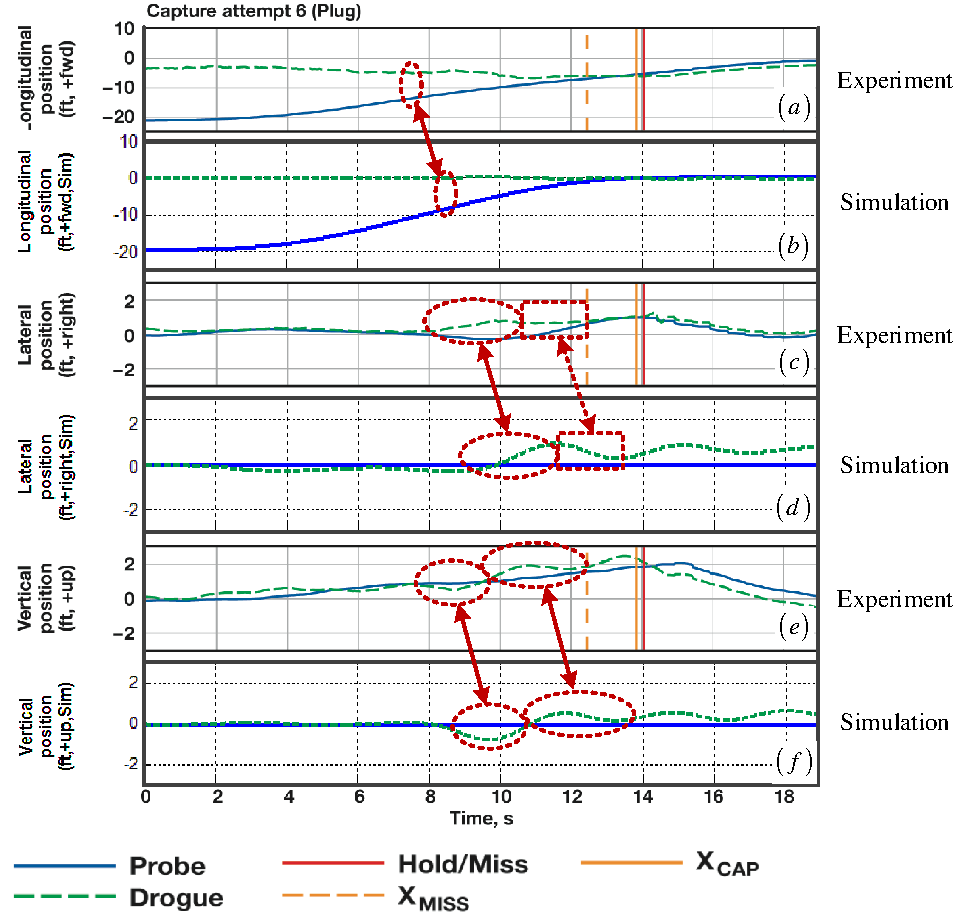
\includegraphics[width=0.6\textwidth]{Chap4/fig23.pdf}
%	\caption{Difference in Drogue Displacement with and without HDU}\label{fig4.23}
%\end{figure}
%
%In the absence of the HDU, the pendulum length remains unchanged, as shown in Fig. \ref{fig4.23}(a). Within the equilibrium range, applying a force to the endpoint of the pendulum, apart from the force direction normal to the equilibrium position, will result in a tangential motion of the pendulum due to forces acting in other directions. In a steady state, the hose tends to be in a more horizontal position, causing both ${F_{{\rm{b}}x}}$ and ${F_{{\rm{b}}z}}$ to primarily induce displacement of the drogue along the ${o_{\rm{t}}}{z_{\rm{t}}}$ direction. This also indicates a significant coupling of the drogue's dynamics in the absence of the HDU.
%When the HDU is considered, it adjusts the length of the exposed hose outside the aircraft in response to changes in hose tension, as depicted in Fig. \ref{fig4.23}(b). When the drogue experiences a longitudinal force ${F_{{\rm{b}}x}}$ from the bow wave, the HDU reduces the length of the exposed hose, thereby changing the primary direction of movement of the drogue from downward to forward. It is evident that the HDU modifies the dynamics of the drogue during the docking process.
%
%\subsection{Model of the HDU}
%
%The model of the HDU typically employs a reel model\cite{vassberg_numerical_2004}, and its dynamics can be expressed as follows 
%\begin{equation}\label{eq4.119}
%	\left( {{T_{{\rm{reel}}}} - {T_{{\rm{hose}}}}} \right){r_{{\rm{reel}}}} = {I_{{\rm{reel}}}}{\alpha _{{\rm{reel}}}}
%\end{equation}
%where ${T_{{\rm{reel}}}}$ and ${T_{{\rm{hose}}}}$ represent the tension in the reel and the tension at the upper end of the hose, respectively. Since the direction of force is not analyzed here, scalar magnitudes of tension are used. The symbols ${r_{{\rm{reel}}}}, {I_{{\rm{reel}}}}$ and ${\alpha _{{\rm{reel}}}}$ represent the radius of the reel, moment of inertia, and angular acceleration around its central axis. Furthermore, if the reel is considered as a cylindrical object, one have 
%\begin{equation}\label{eq4.120}
%	{I_{{\rm{reel}}}} = {m_{{\rm{reel}}}}r_{{\rm{reel}}}^2
%\end{equation}
%On the other hand, expressing ${\alpha _{{\rm{reel}}}}$ in terms of linear acceleration 
%\begin{equation}\label{eq4.121}
%	{\alpha _{{\rm{reel}}}} = \frac{{{{\ddot l}_1}}}{{{r_{{\rm{reel}}}}}}
%\end{equation}
%It should be noted that the change in the length of the hose is replaced by the change in the length of the first link. Although from Section 4.2 it can be understood that the one exposed is the $i$-th link, due to the relatively small retraction of the hose during the docking process, extending the original length of the first link appropriately ensures that the first link is always exposed. Of course, the model of variable first link in Section 4.2.5 can also be used, but it involves more complex calculations. Substituting Eqs. (\ref{eq4.120}) and (\ref{eq4.121}) into Eq. (\ref{eq4.119}), the kinematic model of HDU can be obtained as 
%\begin{equation}\label{eq4.122}
%	{\ddot l_1} = \frac{{{T_{{\rm{reel}}}} - {T_{{\rm{hose}}}}}}{{{m_{{\rm{reel}}}}}}
%\end{equation}
%The dynamic model of the HDU is determined by its controller, which will be elaborated on in the next section.
%
%\subsection{HDU Controller and Qualitative Analysis of its Control Effect}
%
%The controller of the HDU adjusts ${T_{{\rm{reel}}}}$ by using the state variables of the hose (such as ${T_{{\rm{hose}}}},{l_1}$ and ${\dot l_1}$) to indirectly control the length of the exposed hose, thereby regulating the hose tension and achieving equilibrium without causing hose whipping phenomenon. Fig. \ref{fig4.24} illustrates the structural diagram of the link-connected hose-drogue model with the inclusion of the HDU.
%
%(1)Two Types of Controllers for HDU
%
%The first type of controller is the one proposed in Refs. \cite{vassberg_numerical_2004,ro_modeling_2010}.
%\begin{equation}\label{eq4.123}
%	{T_{{\rm{reel}}}}\left( t \right) = {T_{{\rm{reel}}}}\left( 0 \right){\left[ {\frac{{{l_1}\left( t \right)}}{{{l_1}\left( 0 \right)}}} \right]^k},0 < {l_1}\left( t \right) \le {l_1}\left( 0 \right)
%\end{equation}
%That is, at $t = 0$, when the hose is just fully extended, ${T_{{\rm{reel}}}}\left( 0 \right)$ represents the tension at that moment, ${l_1}\left( 0 \right)$ is the length of the first link at that moment, and $k \in \mathbb{R}_{+}$ is the parameter of the controller. It can be observed from Eqs. (\ref{eq4.122}) and (\ref{eq4.123}) that when the hose is completely extended (which corresponds to the state at $t = 0$), the controller achieves equilibrium, and there is no change in the hose length.
%\begin{figure}[th]
%	\centering
%	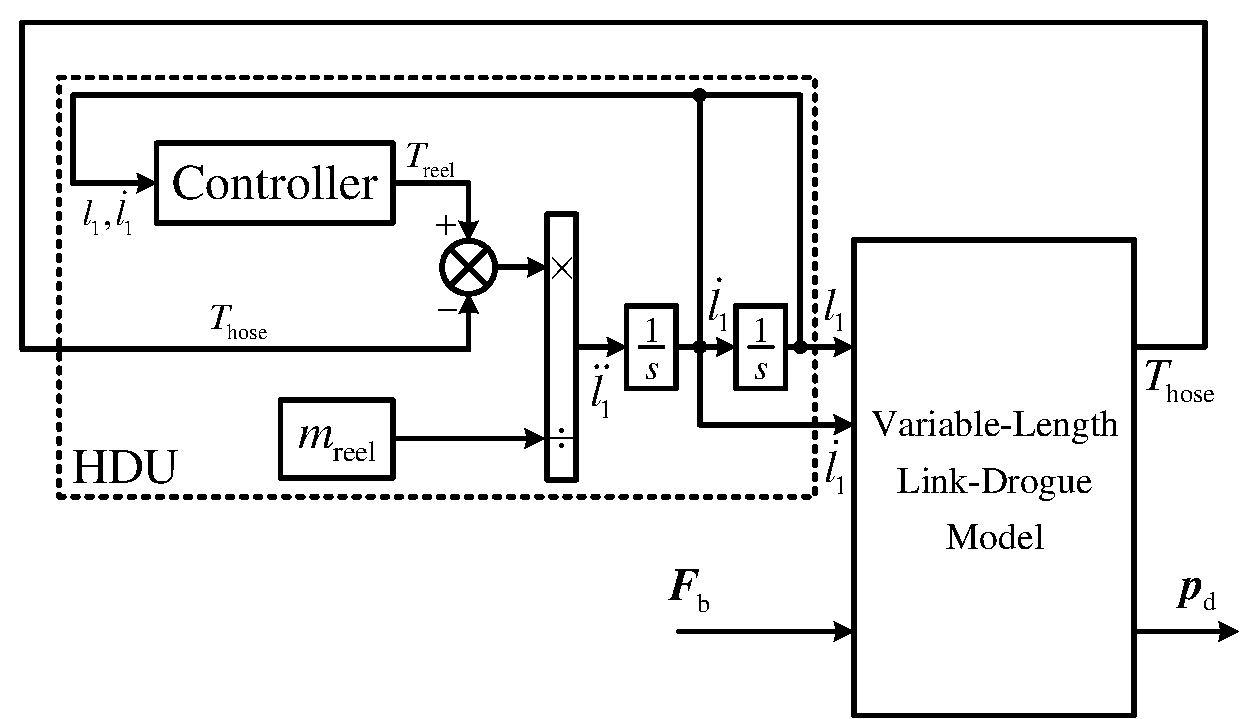
\includegraphics[width=0.7\textwidth]{Chap4/fig24.pdf}
%	\caption{Schematic of link-connected hose-drogue model with HDU}\label{fig4.24}
%\end{figure}
%While the first type of controller does regulate the hose tension, its transient behavior is suboptimal. Therefore, based on the first type of controller, the second type of controller is proposed 
%\begin{equation}\label{eq4.124}
%	{T_{{\rm{reel}}}}\left( t \right) = {T_{{\rm{reel}}}}\left( 0 \right){\left[ {\frac{{{l_1}\left( t \right)}}{{{l_1}\left( 0 \right)}}} \right]^k} + {k_d}{\dot l_1}\left( t \right),0 < {l_1}\left( t \right) \le {l_1}\left( 0 \right)
%\end{equation}
%where ${k_d} \in \mathbb{R}_{+}$. The second type of controller introduces a damping term ${k_d}{\dot l_1}\left( t \right)$, which can effectively improve the transient performance. Furthermore, since we can directly measure the linear velocity of the hose length change, or indirectly obtain the hose length change through the rotation speed of the drum, this controller is easy to implement.
%
%Next, the HDU and the variable-length link-connected hose-drogue model will be used to simulate the control effects of the two types of controllers and analyze the effects of different $k$ values on each type of controller.
%
%(2)Simulation and Qualitative Analysis of Two Types of Controllers
%
%Firstly, establish the simulation model as shown in Fig. \ref{fig4.24}. The basic settings of the simulation environment are outlined in Table \ref{tab4.2}. For the sake of convenience in simulation, some of the parameters listed in Table \ref{tab4.2} have been modified in this chapter's simulations. Additionally, new simulation parameters related to the HDU have been added, as depicted in Table \ref{tab4.3}.
%
%Let the force ${\bm {f}_{\rm{b}}}$ experience a step change from ${\left[ {\begin{array}{*{20}{c}}
%	0&0&0
%\end{array}} \right]^{\rm{T}}}$ to ${\left[ {\begin{array}{*{20}{c}}
%	{75}&0&0
%\end{array}} \right]^{\rm{T}}}$ at 100 seconds. This is done to mimic the force difference in the ${o_{\rm{t}}}{x_{\rm{t}}}$ direction that contributed to the disparities between simulations and experiments in Section 4.3.4. For both the first type of controller and the second type of controller, select the controller parameters as $k = \left\{ {0.3,0.5,1,3} \right\}$, with ${k_d} = 500$ for the second type of controller.
%
%The simulation results are presented in Fig. \ref{fig4.25}. Subfigures (a1)-(a4) depict the control effects of the first type of controller, while subfigures (b1)-(b4) illustrate the control effects of the second type of controller. Through comparison, the following conclusions can be qualitatively drawn:
%
%1) Comparing subfigures (a1)-(a4) and (b1)-(b4) in Fig. \ref{fig4.25}, it can be observed that the first type of controller leads to pronounced oscillations with a longer settling time. In contrast, the second type of controller exhibits significant improvements in both tension adjustment and drogue position control, showing smoother transition dynamics than the first type of controller.
%
%2) Comparing Fig. \ref{fig4.25} (a1) with Fig. \ref{fig4.25} (b1), it can be deduced that the parameter $k$ does not influence the steady-state value of the final hose tension.
%
%3) Comparing Fig. \ref{fig4.25} (a1) with Fig. \ref{fig4.25} (b1), it can be observed that the parameter $k$ significantly affects the retraction length of the hose. When $k$ is smaller, the HDU needs to retract a longer length of the hose to achieve the same steady-state tension value. Conversely, if a minimal change in hose length is desired, a larger $k$ value can be chosen.
%
%4) A larger value of $k$ brings about a noticeable negative effect, which makes the HDU-hose-drogue system unstable. This can be observed from Figs. \ref{fig4.25} (a1)-(a4), where the adjustment time of various quantities significantly increases with the increase in $k$. In fact, for the first type of controller with $k = 4$, the outputs of various quantities have already diverged. In contrast, comparing Figs. \ref{fig4.25} (b1)-(b4) reveals that the second type of controller shows significant improvement in addressing this phenomenon.
%
%5) From Figs. \ref{fig4.25} (a3) and (a4) and Figs \ref{fig4.25} (b3) and (b4), it can be observed that the parameter $k$ indirectly influences the dynamics of the drogue in various directions by affecting the length of the hose. This characteristic will be further discussed in the subsequent sections of this chapter.
%
%% Table generated by Excel2LaTeX from sheet 'Sheet1'
%\begin{table}[htbp]
%	\centering
%	\caption{Parameters Used in HDU Simulation}
%	  \begin{tabular}{|l|c|c|}
%		\hline Parameters    & Values & Units \\ \hline
%		Number of Link Segments $N$  & $10$    & - \\ \hline
%		Initial Length of the First Link ${l_1}\left( 0 \right)$ & $2$     & $m$ \\ \hline
%		Lengths of the Remaining Links ${l_j}\left( 0 \right),j = 2,3, \ldots ,N$ & $13/9$  & $m$ \\ \hline
%		The Mass of the Reel ${m_{{\rm{reel}}}}$& $68$    & $kg$ \\ \hline
%		Initial Tension of the Reel  & 1610  & $N$ \\ \hline
%	  \end{tabular}%
%	\label{tab4.4}%
%\end{table}%
%\begin{figure}[th]
%	\centering
%	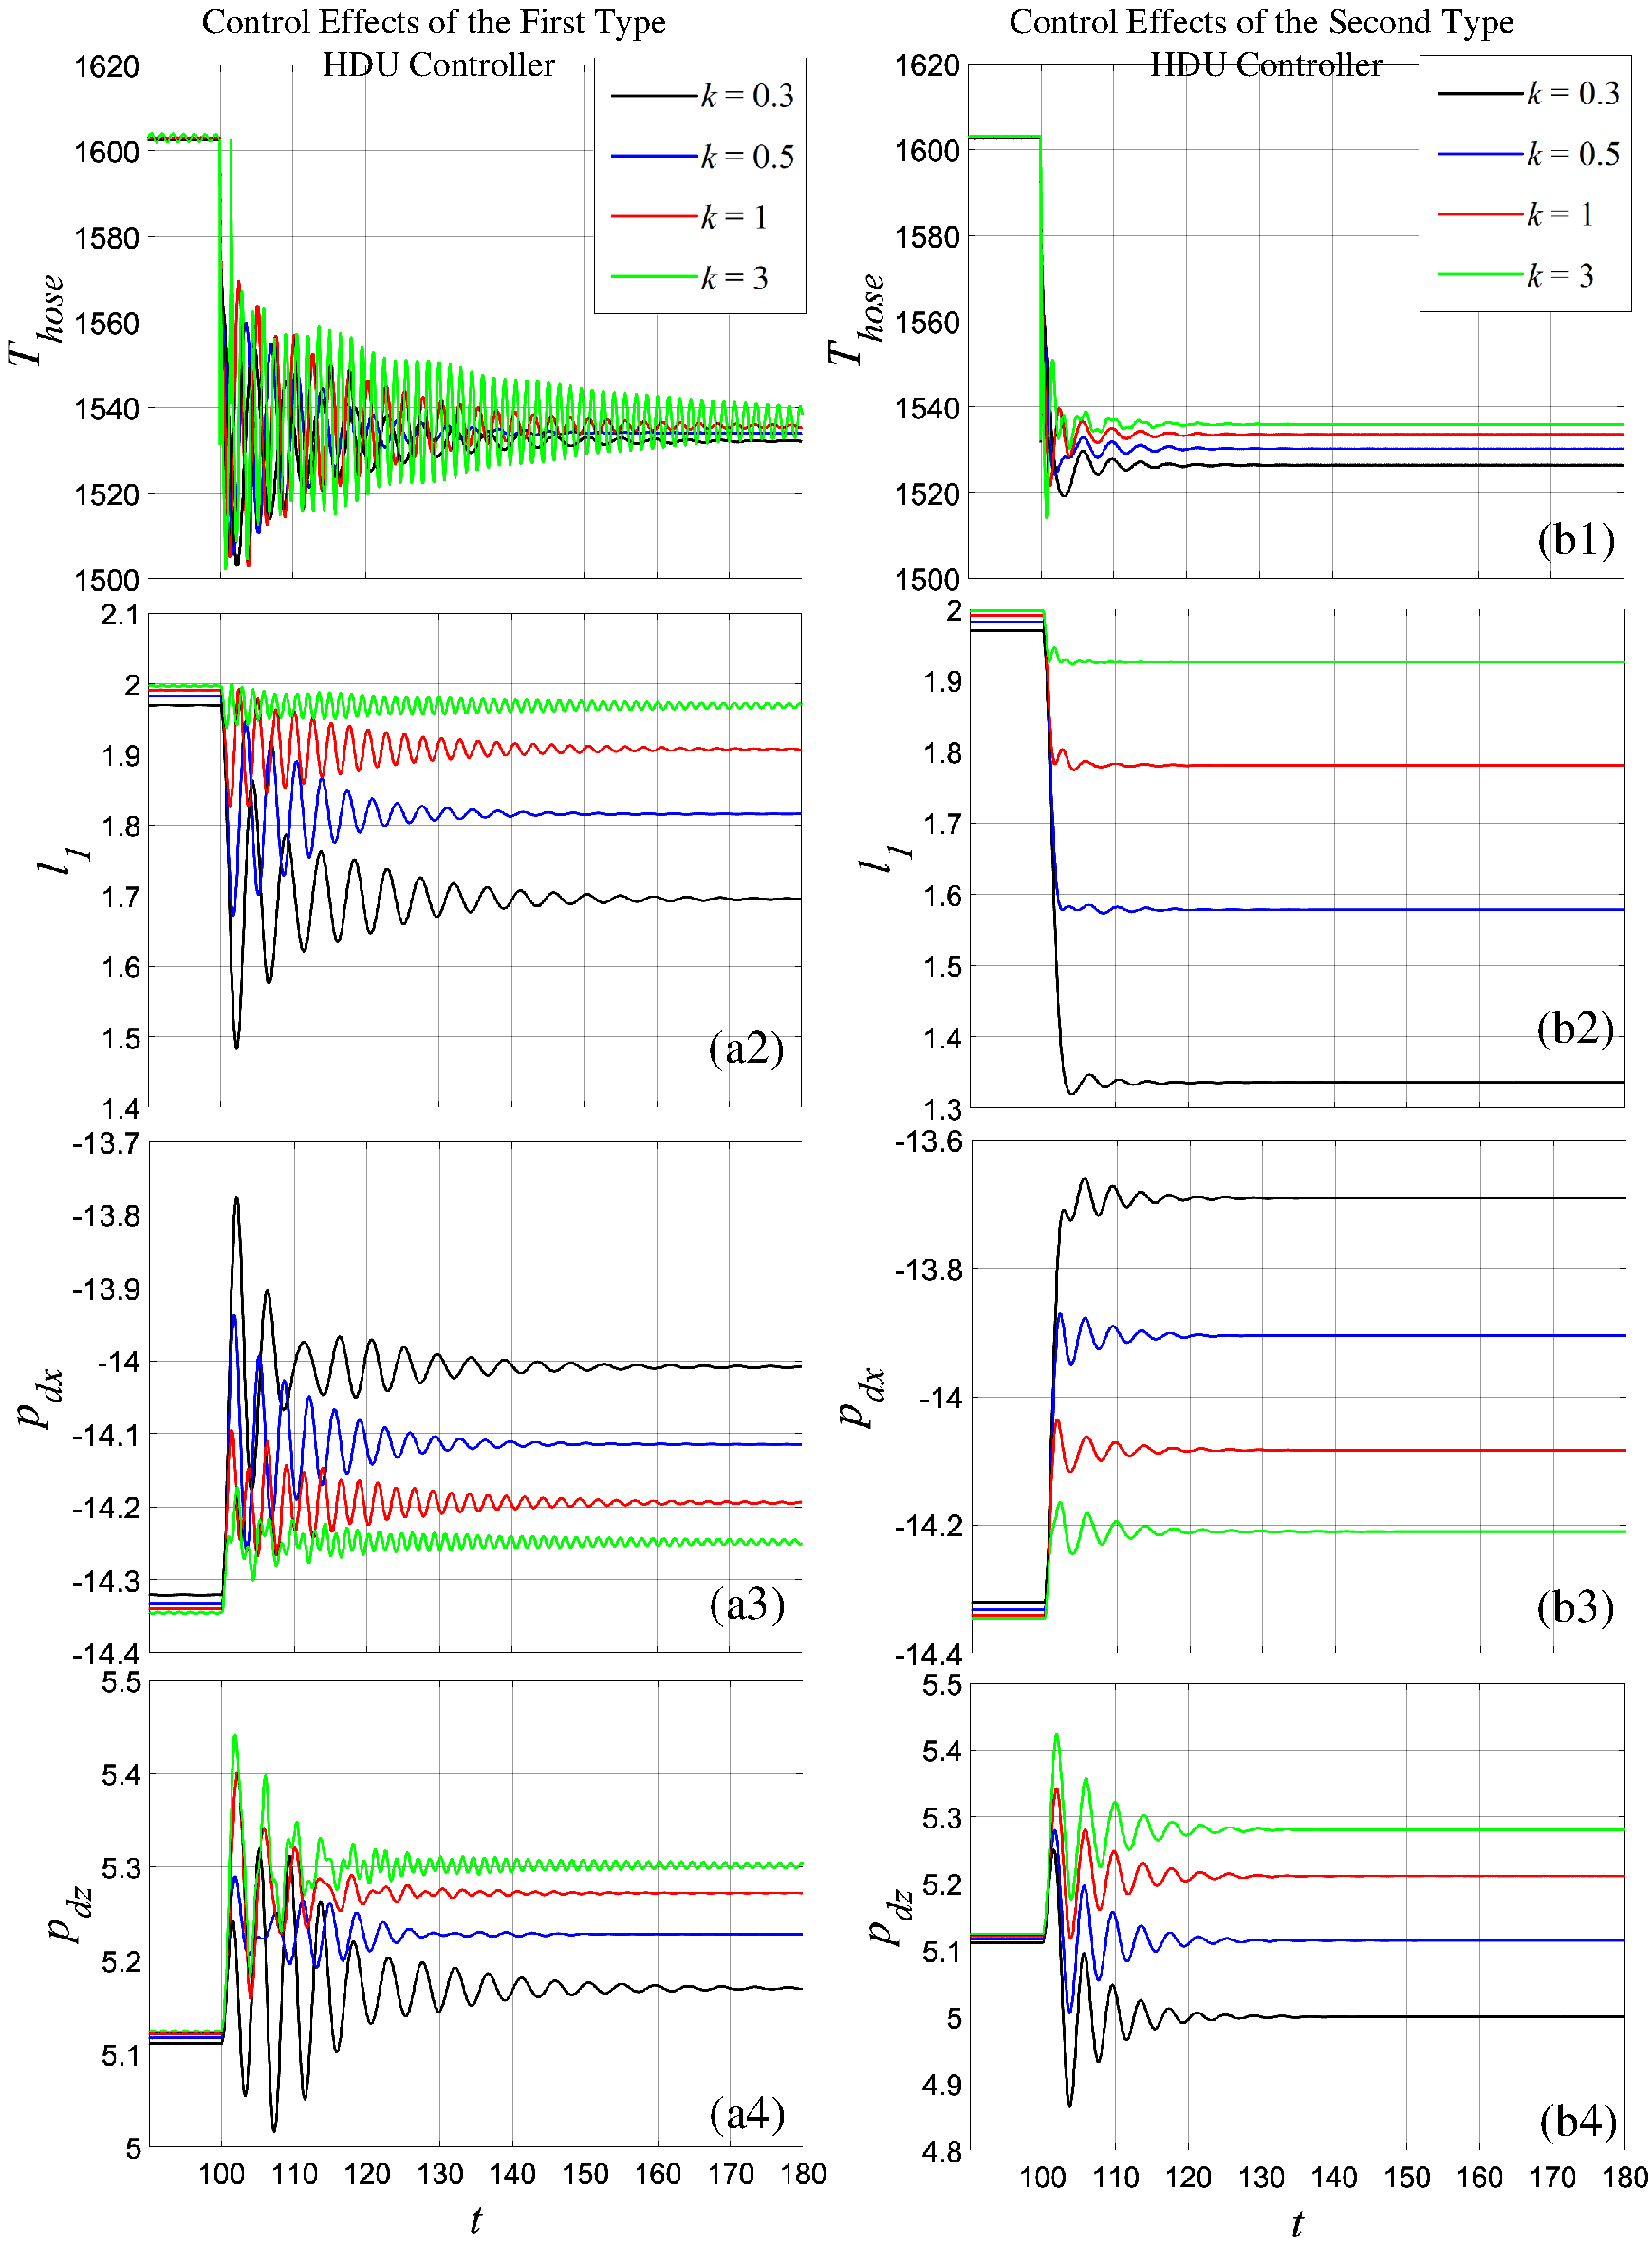
\includegraphics[width=0.7\textwidth]{Chap4/fig25.pdf}
%	\caption{Control Effects of Two Types of HDU Controllers}\label{fig4.25}
%\end{figure} 
%\section{Simplified Drogue Dynamic Model}
%
%Regardless of whether the link-connected hose-drogue model includes the HDU, the model is too complex. As described in Section 4.2, to better simulate the dynamics of the hose, a significant number of links are required, with each link having multiple state variables such as ${\alpha _j},{\beta _j},{\dot \alpha _j},{\dot \beta _j},{l_j},{\dot l_j}$, etc. This complexity results in a high-order link-connected hose-drogue model. Additionally, the presence of nonlinear operations in model calculations further increases its complexity. However, when designing a docking controller, only the dynamics of the drogue are concerned with, and the dynamics of other links become redundant. Therefore, this section aims to simplify the link-connected hose-drogue model in order to obtain a model that solely expresses the dynamics of the drogue. This simplified model is referred to as the drogue dynamics model. It has a lower order and is suitable for controller design in subsequent chapters. Furthermore, it allows for quantitative analysis of the drogue's dynamics under different HDU models.
%
%\subsection{Problem Description and Modeling Approach for Drogue Dynamic Model}
%
%(1) Problem Description for Drogue Dynamic Model
%
%In Section 4.3.1, the link-connected hose-drogue model was represented using Eq. (\ref{eq4.99}). If taking the HDU model into account, with the drogue's forces as inputs and the drogue's position as output, the system can be expressed as follows 
%\begin{equation}\label{eq4.125}
%	\left\{ \begin{aligned}
%		&{{ {\dot {\bf{x}}}}_{{\rm{reel}}}} = { {{\bm{f}}}_{{\rm{reel}}}}\left( {{ {{\bf{x}}}_{{\rm{reel}}}},{ {{\bf{x}}}_{\rm{h}}}} \right)\\
%		&{{ {\dot {\bf{x}}}}_{\rm{h}}} = { {{\bm{f}}}_{{\rm{h0}}}}\left( {{ {{\bf{x}}}_{\rm{h}}},{ {{\bf{x}}}_{\rm{d}}}, {{\mathbf{v}}}_{{\rm{t/w}}}^{\rm{g}},h_{\rm{t}}^{\rm{g}}} \right)\\
%		&{{ {\dot {\bm{x}}}}_{\rm{d}}} = { {{\bm{f}}}_{{\rm{d0}}}}\left( {{ {{\bm{x}}}_{\rm{h}}},{ {{\bf{x}}}_{\rm{d}}}, {{\mathbf{v}}}_{{\rm{t/w}}}^{\rm{g}},h_{\rm{t}}^{\rm{g}},{ {{\bf{F}}}_{\rm{b}}}} \right)\\
%		&{ {{\bf{p}}}_{\rm{d}}} = { {{\bm{f}}}_y}\left( {{ {{\bf{x}}}_{\rm{h}}},{ {{\bf{x}}}_{\rm{d}}}} \right)
%		\end{aligned} \right.
%\end{equation}
%where ${ {{\bf{x}}}_{{\rm{reel}}}}$ represents the state variables of the HDU, and ${ {{\bm{f}}}_{{\rm{reel}}}}$ represents the function related to the dynamics of the HDU as described in Section 4.4. Under a constant tanker altitude ${h_0}$ and airspeed ${ \bm{v}_0}$, the model is simplified to 
%\begin{equation}\label{eq4.126}
%	\left\{ \begin{aligned}
%		&{{ {\dot {\bf{x}}}}_{{\rm{reel}}}} = { {{\bm{f}}}_{{\rm{reel}}}}\left( {{ {{\bf{x}}}_{{\rm{reel}}}},{ {{\bf{x}}}_{\rm{h}}}} \right)\\
%		&{{ {\dot {\bf{x}}}}_{\rm{h}}} = { {{\bm{f}}}_{\rm{h}}}\left( {{ {{\bf{x}}}_{{\rm{reel}}}},{ {{\bf{x}}}_{\rm{h}}},{ {{\bf{x}}}_{\rm{d}}}} \right)\\
%		&{{ {\dot {\bf{x}}}}_{\rm{d}}} = { {{\bm{f}}}_{\rm{d}}}\left( {{ {{\bm{x}}}_{\rm{h}}},{ {{\bf{x}}}_{\rm{d}}},{ {{\mathbf{F}}}_{\rm{b}}}} \right)\\
%		&{ {{\bf{p}}}_{\rm{d}}} = { {{\bm{f}}}_y}\left( {{ {{\bf{x}}}_{\rm{h}}},{ {{\bf{x}}}_{\rm{d}}}} \right)
%		\end{aligned} \right.
%\end{equation}
%where ${ {{\bm{f}}}_{\rm{h}}}\left( {{ {{\bf{x}}}_{\rm{h}}},{ {{\bf{x}}}_{\rm{d}}}} \right) \triangleq { {{\bm{f}}}_{{\rm{h0}}}}\left( {{ {{\bf{x}}}_{\rm{h}}},{ {{\bf{x}}}_{\rm{d}}},{ {{\bf{v}}}_0},{h_0}} \right),{ {{\bm{f}}}_{\rm{d}}}\left( {{ {{\bf{x}}}_{\rm{h}}},{ {{\bf{x}}}_{\rm{d}}},{ {{\bf{F}}}_{\rm{b}}}} \right) \triangleq { {{\bm{f}}}_{{\rm{d0}}}}\left( {{ {{\bf{x}}}_{\rm{h}}},{ {{\bf{x}}}_{\rm{d}}},{ {{\bf{v}}}_0},{h_0},{ {{\bf{F}}}_{\rm{b}}}} \right)$. Then, for each set of $\left( {{ {{\bf{v}}}_0},{h_0}} \right)$, and when the system (\ref{eq4.126}) is subjected to zero input (i.e., ${ {{\bf{F}}}_{\rm{b}}} = {\bf{0}}$), the system will reach a steady-state position. Denote the state of the system at this time as the equilibrium state 
%\begin{equation}\label{eq4.127}
%	{ {{\bf{x}}}_{{\rm{reel}}}} =  {{\bf{x}}}_{{\rm{reel}}}^*,{ {{\bf{x}}}_{\rm{h}}} =  {{\bf{x}}}_{\rm{h}}^{\rm{*}},{ {{\bf{x}}}_{\rm{d}}} =  {{\bf{x}}}_{\rm{d}}^{\rm{*}}
%\end{equation}
%At this moment, the system satisfies the equation 
%\begin{equation}\label{eq4.128}
%	\left\{ \begin{aligned}
%		 &{\dot {\bf{x}}}_{{\rm{reel}}}^* = { {{\bm{f}}}_{{\rm{reel}}}}\left( { {{\bf{x}}}_{{\rm{reel}}}^*, {{\bf{x}}}_{\rm{h}}^{\rm{*}}} \right)\\
%		 &{\dot {\bf{x}}}_{\rm{h}}^{\rm{*}} = { {{\bm{f}}}_{\rm{h}}}\left( { {{\bf{x}}}_{{\rm{reel}}}^*, {{\bf{x}}}_{\rm{h}}^{\rm{*}}, {{\bf{x}}}_{\rm{d}}^{\rm{*}}} \right)\\
%		 &{\dot {\bf{x}}}_{\rm{d}}^{\rm{*}} = { {{\bm{f}}}_{\rm{d}}}\left( { {{\bf{x}}}_{\rm{h}}^{\rm{*}}, {{\bf{x}}}_{\rm{d}}^{\rm{*}},{\bf{0}}} \right)\\
%		 &{{\bf{p}}}_{\rm{d}}^{\rm{*}} = { {{\bm{f}}}_y}\left( { {{\bf{x}}}_{\rm{h}}^{\rm{*}}, {{\bf{x}}}_{\rm{d}}^{\rm{*}}} \right)
%		\end{aligned} \right.
%\end{equation}
%Linearizing the system (\ref{eq4.126}) at the equilibrium point (\ref{eq4.128}), we can obtain 
%\begin{equation}\label{eq4.129}
%	\left\{ \begin{aligned}
%		\left[ {\begin{array}{*{20}{c}}
%		{\Delta {{ {\dot {\bf{x}}}}_{{\rm{reel}}}}}\\
%		{\Delta {{ {\dot {\bf{x}}}}_{\rm{h}}}}\\
%		{\Delta {{ {\dot {\bf{x}}}}_{\rm{d}}}}
%		\end{array}} \right] &= \underbrace {\left[ {\begin{array}{*{20}{c}}
%		{{{\bf{A}}_{11}}}&{{{\bf{A}}_{12}}}&{\bf{0}}\\
%		{{{\bf{A}}_{21}}}&{{{\bf{A}}_{22}}}&{{{\bf{A}}_{23}}}\\
%		{\bf{0}}&{{{\bf{A}}_{32}}}&{{{\bf{A}}_{33}}}
%		\end{array}} \right]}_{\bf{A}}\left[ {\begin{array}{*{20}{c}}
%		{\Delta { {{\bf{x}}}_{{\rm{reel}}}}}\\
%		{\Delta { {{\bf{x}}}_{\rm{h}}}}\\
%		{\Delta { {{\bf{x}}}_{\rm{d}}}}
%		\end{array}} \right] + \underbrace {\left[ {\begin{array}{*{20}{c}}
%		{\bf{0}}\\
%		{\bf{0}}\\
%		{{{\bf{B}}_3}}
%		\end{array}} \right]}_{\bf{B}}{\bf {F}_{\rm{b}}}{\rm{ + }}\left[ {\begin{array}{*{20}{l}}
%		{o\left( {\Delta { {{\bm{x}}}_{{\rm{reel}}}},\Delta { {{\bf{x}}}_{\rm{h}}}} \right)}\\
%		{o\left( {\Delta { {{\bm{x}}}_{{\rm{reel}}}},\Delta { {{\bf{x}}}_{\rm{h}}},\Delta { {{\bm{x}}}_{\rm{d}}}} \right)}\\
%		{o\left( {\Delta { {{\bm{x}}}_{\rm{h}}},\Delta { {{\bf{x}}}_{\rm{d}}},{ {F}_{\rm{b}}}} \right)}
%		\end{array}} \right]\\
%		\Delta { {{\bf{p}}}_{\rm{d}}} &= \underbrace {\left[ {\begin{array}{*{20}{c}}
%		{\bf{0}}&{{{\bf{C}}_2}}&{{{\bf{C}}_3}}
%		\end{array}} \right]}_{\bf{C}}\left[ {\begin{array}{*{20}{c}}
%		{\Delta { {{\bf{x}}}_{{\rm{reel}}}}}\\
%		{\Delta { {{\bf{x}}}_{\rm{h}}}}\\
%		{\Delta { {{\bf{x}}}_{\rm{d}}}}
%		\end{array}} \right] + o\left( {\Delta { {{\bf{x}}}_{\rm{h}}},\Delta { {{\bf{x}}}_{\rm{d}}}} \right)
%		\end{aligned} \right.
%\end{equation}
%where
%\begin{equation}\label{eq4.130}
%	\begin{array}{*{20}{l}}
%		{{{\bf{A}}_{11}}{\rm{ = }}{{\left. {\frac{{\partial { {{\bm{f}}}_{{\rm{reel}}}}}}{{\partial { {{\bf{x}}}_{{\rm{reel}}}}}}} \right|}_{\scriptstyle{ {{\bf{x}}}_{{\rm{reel}}}} =  {{\bf{x}}}_{{\rm{reel}}}^*\hfill\atop
%		\scriptstyle{ {{\bf{x}}}_{\rm{h}}} =  {{\bf{x}}}_{\rm{h}}^{\rm{*}}\hfill}},}&{{{\bf{A}}_{12}}{\rm{ = }}{{\left. {\frac{{\partial { {{\bm{f}}}_{{\rm{reel}}}}}}{{\partial { {{\bf{x}}}_{\rm{h}}}}}} \right|}_{\scriptstyle{ {{\bf{x}}}_{{\rm{reel}}}} =  {{\bf{x}}}_{{\rm{reel}}}^*\hfill\atop
%		\scriptstyle{ {{\bf{x}}}_{\rm{h}}} =  {{\bf{x}}}_{\rm{h}}^{\rm{*}}\hfill}},}&{{{\bf{A}}_{21}}{\rm{ = }}{{\left. {\frac{{\partial { {{\bm{f}}}_{\rm{h}}}}}{{\partial { {{\bf{x}}}_{{\rm{reel}}}}}}} \right|}_{\scriptstyle{ {{\bf{x}}}_{{\rm{reel}}}} =  {{\bf{x}}}_{{\rm{reel}}}^*\hfill\atop
%		{\scriptstyle{ {{\bf{x}}}_{\rm{h}}} =  {{\bf{x}}}_{\rm{h}}^{\rm{*}}\hfill\atop
%		\scriptstyle{ {{\bf{x}}}_{\rm{d}}} =  {{\bf{x}}}_{\rm{d}}^{\rm{*}}\hfill}}},}&{{{\bf{A}}_{22}}{\rm{ = }}{{\left. {\frac{{\partial { {{\bm{f}}}_{\rm{h}}}}}{{\partial { {{\bf{x}}}_{\rm{h}}}}}} \right|}_{\scriptstyle{ {{\bf{x}}}_{{\rm{reel}}}} =  {{\bf{x}}}_{{\rm{reel}}}^*\hfill\atop
%		{\scriptstyle{ {{\bf{x}}}_{\rm{h}}} =  {{\bf{x}}}_{\rm{h}}^{\rm{*}}\hfill\atop
%		\scriptstyle{ {{\bf{x}}}_{\rm{d}}} =  {{\bf{x}}}_{\rm{d}}^{\rm{*}}\hfill}}},}\\
%		{{{\bf{A}}_{23}}{\rm{ = }}{{\left. {\frac{{\partial { {f}_{\rm{h}}}}}{{\partial { {{\bf{x}}}_{\rm{d}}}}}} \right|}_{\scriptstyle{ {{\bf{x}}}_{{\rm{reel}}}} =  {{\bf{x}}}_{{\rm{reel}}}^*\hfill\atop
%		{\scriptstyle{ {{\bf{x}}}_{\rm{h}}} =  {{\bf{x}}}_{\rm{h}}^{\rm{*}}\hfill\atop
%		\scriptstyle{ {{\bf{x}}}_{\rm{d}}} =  {{\bf{x}}}_{\rm{d}}^{\rm{*}}\hfill}}},}&{{{\bf{A}}_{32}}{\rm{ = }}{{\left. {\frac{{\partial { {{\bm{f}}}_{\rm{d}}}}}{{\partial { {{\bf{x}}}_{\rm{h}}}}}} \right|}_{\scriptstyle{ {{\bf{x}}}_{\rm{h}}} =  {{\bf{x}}}_{\rm{h}}^{\rm{*}}\hfill\atop
%		{\scriptstyle{ {{\bf{x}}}_{\rm{d}}} =  {{\bf{x}}}_{\rm{d}}^{\rm{*}}\hfill\atop
%		\scriptstyle{ {F}_{\rm{b}}} = 0\hfill}}},}&{{{\bf{A}}_{33}}{\rm{ = }}{{\left. {\frac{{\partial { {{\bm{f}}}_{\rm{d}}}}}{{\partial { {{\bf{x}}}_{\rm{d}}}}}} \right|}_{\scriptstyle{ {{\bf{x}}}_{\rm{h}}} =  {{\bf{x}}}_{\rm{h}}^{\rm{*}}\hfill\atop
%		{\scriptstyle{ {{\bf{x}}}_{\rm{d}}} =  {{\bf{x}}}_{\rm{d}}^{\rm{*}}\hfill\atop
%		\scriptstyle{ {F}_{\rm{b}}} = 0\hfill}}},}&{{{\bf{B}}_3}{\rm{ = }}{{\left. {\frac{{\partial { {{\bm{f}}}_{\rm{d}}}}}{{\partial { {{\bm{f}}}_{\rm{b}}}}}} \right|}_{\scriptstyle{ {{\bf{x}}}_{\rm{h}}} =  {{\bf{x}}}_{\rm{h}}^{\rm{*}}\hfill\atop
%		{\scriptstyle{ {{\bf{x}}}_{\rm{d}}} =  {{\bf{x}}}_{\rm{d}}^{\rm{*}}\hfill\atop
%		\scriptstyle{ {F}_{\rm{b}}} = 0\hfill}}},}\\
%		{{{\bf{C}}_2}{\rm{ = }}{{\left. {\frac{{\partial { {{\bm{f}}}_y}}}{{\partial { {{\bf{x}}}_{\rm{h}}}}}} \right|}_{\scriptstyle{ {{\bf{x}}}_{\rm{h}}} =  {{\bf{x}}}_{\rm{h}}^{\rm{*}}\hfill\atop
%		\scriptstyle{ {{\bf{x}}}_{\rm{d}}} =  {{\bf{x}}}_{\rm{d}}^{\rm{*}}\hfill}},}&{{{\bf{C}}_3}{\rm{ = }}{{\left. {\frac{{\partial { {{\bm{f}}}_y}}}{{\partial { {{\bf{x}}}_{\rm{d}}}}}} \right|}_{\scriptstyle{ {{\bf{x}}}_{\rm{h}}} =  {{\bf{x}}}_{\rm{h}}^{\rm{*}}\hfill\atop
%		\scriptstyle{ {{\bf{x}}}_{\rm{d}}} =  {{\bf{x}}}_{\rm{d}}^{\rm{*}}\hfill}}}&{}&{}
%		\end{array}
%\end{equation}
%and $\Delta { {{\bf{x}}}_{{\rm{reel}}}} = { {{\bf{x}}}_{{\rm{reel}}}} -  {{\bf{x}}}_{{\rm{reel}}}^*,\Delta { {{\bf{x}}}_{\rm{h}}} = { {{\bf{x}}}_{\rm{h}}} -  {{\bf{x}}}_{\rm{h}}^*,\Delta { {{\bf{x}}}_{\rm{d}}} = { {{\bf{x}}}_{\rm{d}}} -  {{\bf{x}}}_{\rm{d}}^*,\Delta { {{\bf{p}}}_{\rm{d}}} = { {{\bf{p}}}_{\rm{d}}} -  {{\bf{p}}}_{\rm{d}}^{\rm{*}}$, according to the drogue equilibrium coordinate system, it can be observed that $\Delta { {{\bf{p}}}_{\rm{d}}} =  {{\bf{p}}}_{\rm{d}}^{\rm{e}}$, and $o(\cdot)$ represents higher-order infinitesimal terms in the linearization. Since the changes in the state of the hose and the drogue are relatively small during the docking process, i.e., $\Delta { {{\bf{x}}}_{{\rm{reel}}}},\Delta { {{\bf{x}}}_{\rm{h}}}$ and $\Delta { {{\bf{x}}}_{\rm{d}}}$ are infinitesimal terms that can be neglected. Additionally, if the subsequent model simplification can be validated through the process described in section 4.5.4, it would also indicate the reasonableness of omitting infinitesimal terms here. After neglecting infinitesimal terms, the system (\ref{eq4.129}) becomes a linear system. Subsequently, through Laplace transformation, the transfer function of this linear system can be expressed as 
%\begin{equation}\label{eq4.131}
%	 {{\bf{p}}}_{\rm{d}}^{\rm{e}}\left( s \right) = \underbrace {{\bf{C}}{{\left( {s{\bf{I}} - {\bf{A}}} \right)}^{ - 1}}{\bf{B}}}_{{{\bf{G}}_{\rm{d}}}\left( s \right)}{ {{\bf{F}}}_{\rm{b}}}\left( s \right)
%\end{equation}
%This equation is commonly referred to as the drogue dynamic model.
%
%(2) Modeling Approach for Drogue Dynamic Model
%
%The model (\ref{eq4.131}) includes ${{\bf{G}}_{\rm{d}}}\left( s \right)$, which represents the drogue's dynamics. Next, system identification methods will be used to obtain ${{\bf{G}}_{\rm{d}}}\left( s \right)$, and the following steps outline this process:
%
%1) Utilize axial force to infer the coupling relationships among different channels, and then obtain the basic form of ${{\bf{G}}_{\rm{d}}}\left( s \right)$.
%
%2) Employ Generalized Binary Noise (GBN) as an input to excite the system and identify system parameters.
%
%3) Validate the identified results using a Chirp Signal.
%
%In Sections 4.5.2-4.5.4, we will combine an example of a fixed-length link-connected model to explain the above process. The object to be identified in this example is the same as the one in Section 4.2.5. The obtained drogue dynamic model can be analyzed and compared with the later derived link-connected hose-drogue model with HDU.
%
%\subsection{Speculation on the Form of ${{\bf{G}}_{\rm{d}}}\left( s \right)$}
%
%Five simulations are conducted, each applying an axial force in a different direction to ${\bf{F}_{\rm{b}}}$. The forces were as follows  ${\bf{F}_{{\rm{b}}x{\rm{ + }}}} = {\left[ {\begin{array}{*{20}{c}}
%	{50}&0&0
%\end{array}} \right]^{\rm{T}}}$, ${\bf{F}_{{\rm{b}}y{\rm{ + }}}} = {\left[ {\begin{array}{*{20}{c}}
%		0&{50}&0
%\end{array}} \right]^{\rm{T}}}$, ${\bf{F}_{{\rm{b}}y - }} = {\left[ {\begin{array}{*{20}{c}}
%			0&{ - 50}&0
%\end{array}} \right]^{\rm{T}}}$, ${\bf{F}_{{\rm{b}}z{\rm{ + }}}} = {\left[ {\begin{array}{*{20}{c}}
%				0&0&{50}
%\end{array}} \right]^{\rm{T}}}$, ${\bf{F}_{{\rm{b}}z{\rm{ + }}}} = {\left[ {\begin{array}{*{20}{c}}
%					0&0&{ - 50}
%\end{array}} \right]^{\rm{T}}}$. The reason for not using forces in the ${\bf{F}_{{\rm{b}}x - }}$ direction for simulation is that, under normal circumstances, the receiver does not generate disturbances in the negative direction against the drogue. The choice of an amplitude of $50 N$ is because the maximum bow wave effect during the docking process is around $100 N$, and $50 N$ serves as a representative intermediate value for the bow wave effect. The results of these five simulations are presented in Table \ref{tab4.4}. In the table, $(\cdot)_\text{max}$ represents the maximum drift position of the drogue in the current simulation, while $(\cdot)_\text{final}$ represents the final drift position of the drogue in the current simulation.
%
%According to Table \ref{tab4.4}, the following conclusions can be drawn: 1) The $x$ and $z$ channels are coupled. 2) It can be assumed that the $y$ channel is decoupled from $x$ and $z$ channels, as the effects of ${\bf{F}_{{\rm{b}}y{\rm{ + }}}}$ and ${\bf{F}_{{\rm{b}}y - }}$ on ${x_{{d /t}}}$ and ${z_{{d /t}}}$ are much smaller than the forces in other directions. Therefore, the basic form of ${{\bf{G}}_{\rm{d}}}\left( s \right)$ can be obtained as follows 
%\begin{equation}\label{eq4.132}
%	{{\bf{G}}_{\rm{d}}}\left( s \right) = \left[ {\begin{array}{*{20}{c}}
%		{{G_{xx}}\left( s \right)}&0&{{G_{xz}}\left( s \right)}\\
%		0&{{G_{yy}}\left( s \right)}&0\\
%		{{G_{zx}}\left( s \right)}&0&{{G_{zz}}\left( s \right)}
%		\end{array}} \right]
%\end{equation}
%Additionally, in Section 4.2.5, it has been mentioned that the inherent dynamics of the drogue are of second order. Therefore, it can be inferred that the elements within ${{\bf{G}}_{\rm{d}}}\left( s \right)$ are also of second order.
%% Table generated by Excel2LaTeX from sheet 'Sheet1'
%\begin{table}[htbp]
%	\centering
%	\caption{Drift positions of the drogue under the influence of Fb in different directions}
%	  \begin{tabular}{|c|c|c|c|c|c|}
%		\hline \diagbox{${\bm{p}_{{d /t}}}$}{${\bf{F}_{\rm{b}}}$}& ${\bf{F}_{{\rm{b}}x{\rm{ + }}}}$ & ${\bf{F}_{{\rm{b}}y{\rm{ + }}}}$ &   ${\bf{F}_{{\rm{b}}y - }}$    &   ${\bf{F}_{{\rm{b}}z{\rm{ + }}}}$    & ${\bf{F}_{{\rm{b}}z - }}$ \\\hline
%			${\left( {{x_{{d /t}}}} \right)_{\max }}$& 0.07  & 0.015 & 0.015 & 0.204 & 0.177 \\\hline
%			${\left( {{x_{{d/t}}}} \right)_{{\rm{final}}}}$& 0.04  & 0.005 & 0.005 & 0.109 & 0.105 \\\hline
%			${\left( {{y_{{d/t}}}} \right)_{\max }}$& 0     & 0.724 & -0.724 & 0     & 0 \\\hline
%			${\left( {{y_{{d / t}}}} \right)_{{\rm{final}}}}$& 0     & 0.41  & -0.41 & 0     & 0 \\\hline
%			${\left( {{z_{{d/ t}}}} \right)_{\max }}$& 0.199 & -0.012 & -0.012 & 0.56  & -0.588 \\\hline
%			${\left( {{z_{{d / t}}}} \right)_{{\rm{final}}}}$& 0.115 & -0.004 & -0.004 & 0.324 & -0.447 \\\hline
%	  \end{tabular}%
%	\label{tab4.5}%
%\end{table}%
%  
%\subsection{System identification of the link-connected hose-drogue model}
%
%Using a GBN (Generalized Binary Noise) signal with an amplitude of $50 N$ to excite the system, as shown in Fig. \ref{fig4.26}, the parameters within ${{\bf{G}}_{\rm{d}}}\left( s \right)$ are identified using the Output-Error (OE) model \cite{ljung_system_1998}. The results can be obtained as follows 
%\begin{equation}\label{eq4.133}
%	\left\{ \begin{array}{c}
%		{G_{xx}}\left( s \right){\rm{ = }}\frac{{{\rm{0}}{\rm{.002185}}}}{{{s^2} + {\rm{0}}{\rm{.3071}}s + {\rm{2}}{\rm{.682}}}}\\
%		{G_{xz}}\left( s \right){\rm{ = }}\frac{{{\rm{0}}{\rm{.006169}}}}{{{s^2} + {\rm{0}}{\rm{.3013}}s + {\rm{2}}{\rm{.689}}}}\\
%		{G_{yy}}\left( s \right){\rm{ = }}\frac{{{\rm{0}}{\rm{.01712}}}}{{{s^2} + {\rm{0}}{\rm{.2422}}s + {\rm{2}}{\rm{.081}}}}\\
%		{G_{zx}}\left( s \right){\rm{ = }}\frac{{{\rm{0}}{\rm{.005824}}}}{{{s^2} + {\rm{0}}{\rm{.3223}}s + {\rm{2}}{\rm{.687}}}}\\
%		{G_{zz}}\left( s \right){\rm{ = }}\frac{{{\rm{0}}{\rm{.01782}}}}{{{s^2} + {\rm{0}}{\rm{.3391}}s + {\rm{2}}{\rm{.687}}}}
%		\end{array} \right..
%\end{equation}
%
%\subsection{Frequency sweep verification}
%
%A frequency sweep signal is simultaneously applied to both the link-connected hose-drogue model (Equation \ref{eq4.126}) and the drogue dynamics model (Equation \ref{eq4.131}), as shown in Fig. \ref{fig4.27}. By comparing the output results of the two systems, the simulation results are presented in Fig. \ref{fig4.28}. The curves in Fig. \ref{fig4.28}(b) are obtained by subtracting the two dashed lines from Fig. \ref{fig4.28}(a). The frequency sweep signal is a signal with a fixed amplitude and a frequency that uniformly increases from ${\zeta _0}$ to ${\zeta _T}$ over the interval $\left[ {0,T} \right]$, and its mathematical expression is 
%\begin{equation}\label{eq4.134}
%	c\left( t \right) = {{\rm{K}}_c}\sin \left[ {2\pi \left( {{\zeta _0} + \frac{{{\zeta _T} - {\zeta _0}}}{T}t} \right)t} \right]
%\end{equation}
%where ${{\rm{K}}_c} = 50,{\zeta _0} = 0.05Hz,{\zeta _T} = 0.5Hz$ and $T = 200s$.
%\begin{figure}[th]
%	\centering
%	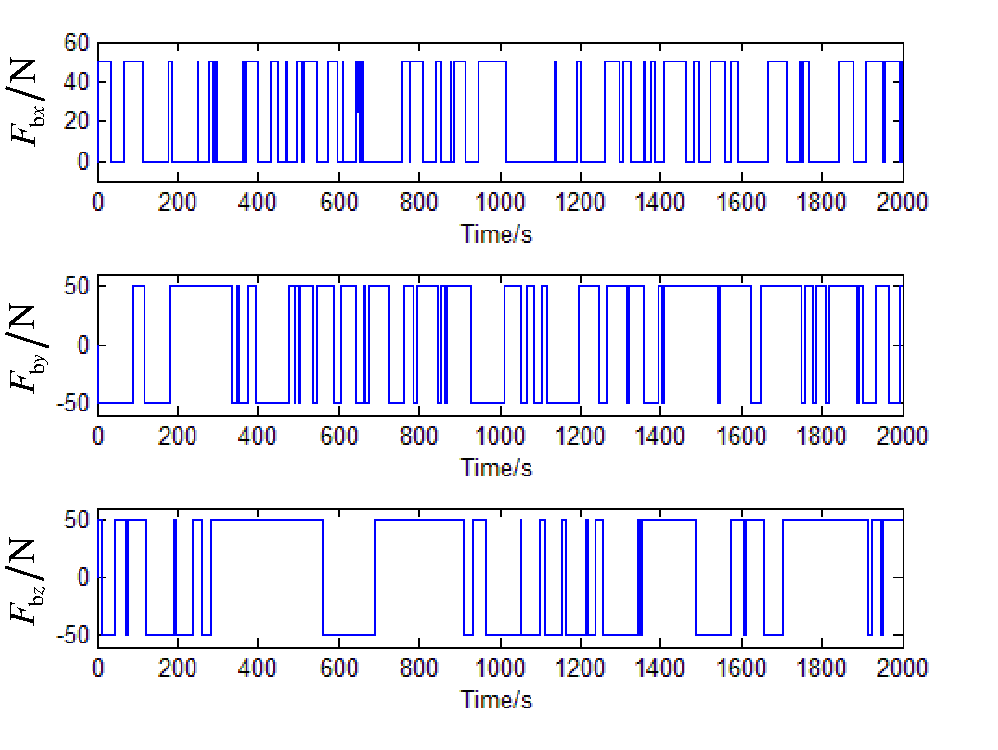
\includegraphics[width=0.7\textwidth]{Chap4/fig26.pdf}
%	\caption{GBN Signal Used to Excite the System}\label{fig4.26}
%\end{figure} 
%\begin{figure}[th]
%	\centering
%	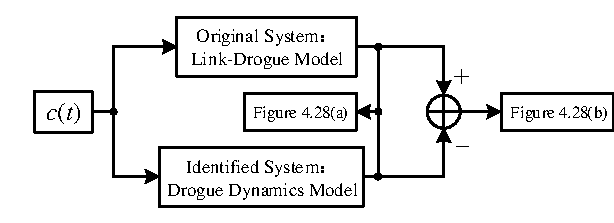
\includegraphics[width=0.7\textwidth]{Chap4/fig27.pdf}
%	\caption{Verification Simulation Framework for Identification Results}\label{fig4.27}
%\end{figure} 
%\begin{figure}[th]
%	\centering
%	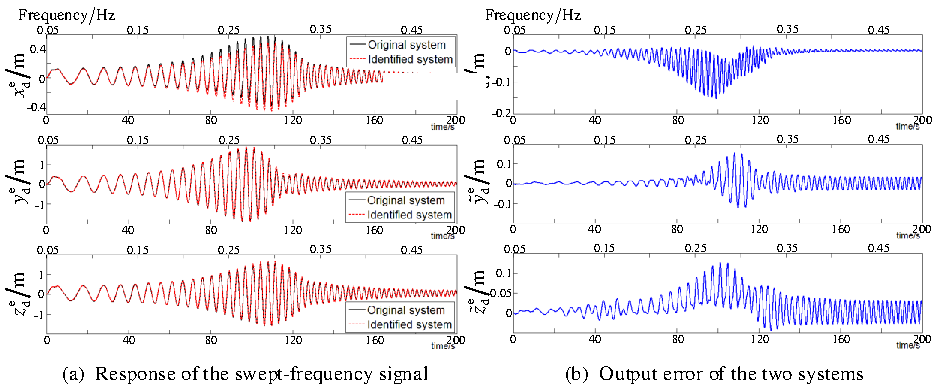
\includegraphics[width=0.7\textwidth]{Chap4/fig28.pdf}
%	\caption{Effectiveness of System Identification}\label{fig4.28}
%\end{figure} 
%From Fig. \ref{fig4.28} (b), it can be observed that the system's tracking error is minimal in the low-frequency range below 0.2 Hz, increases in the mid-frequency range between 0.2 Hz and 0.35 Hz, and remains relatively small in the high-frequency range above 0.35 Hz. The outputs $y_{\rm{d}}^{\rm{e}}$ and $z_{\rm{d}}^{\rm{e}}$ from both models are very close to each other, while the performance of $x_{\rm{d}}^{\rm{e}}$ is relatively poorer. This is mainly due to the higher nonlinearity exhibited by the link-connected hose-drogue model when subjected to ${\bf{F}_{{\rm{b}}x - }}$, which occurs rarely in actual docking scenarios. Therefore, the identified drogue dynamics model effectively captures the drogue dynamics of the link-connected hose-drogue model.
%
%It should be noted that the above model was derived under the assumption of no crosswind or minimal crosswind. In the presence of a crosswind, the $y$-axis becomes coupled with the other axes, meaning that all elements within Eq. (\ref{eq4.132}) would be non-zero. However, the drogue dynamics model can still be obtained using the identification method described above. Since the refueling process allows for adjustments in the direction of the aircraft's velocity to minimize the impact of crosswind disturbances, this chapter primarily focuses on the model under the assumption of no crosswind.
%
%\subsection{Dynamic Model of Drogue with HDU and Quantitative Analysis}
%
%Using the system identification steps described in Sections 4.5.2-4.5.4, the simplified drogue dynamics model for the link-connected hose-drogue system with HDU was obtained. The identification results are presented in Table \ref{tab4.5}. The controller choices are as shown in Section 4.3.3: for the first type of HDU controller (\ref{eq4.123}), the parameter is set as $k = 0.5$, and for the second type of HDU controller (\ref{eq4.124}), the parameters are chosen as $k = 0.5$ and ${k_d} = 500$. In the table, the fitness metric is used to represent the identification performance, defined as $1 - {{\left\| {\bm{y} - \bm{\hat y}} \right\|} /{\left\| {\bm{y} - \bm{\bar y}} \right\|}}$, where $\bm{y},\bm{\hat y}$ and $\bm{\bar y}$ represent the output of the original model, the the output of the identification model, and the mean of the output of the original model, respectively.
%
%Unlike the drogue dynamics without considering HDU (Eq. (\ref{eq4.131})), the identification in Table \ref{tab4.5} utilizes a fourth-order model. The reason behind this choice is that the drogue dynamics without HDU are second-order, while the HDU itself introduces an additional second-order dynamics. Hence, a fourth-order model is employed to identify the link-connected hose-drogue system with HDU. Moreover, judging from the fitness values in the identification results, the fourth-order model also performs better than the second-order model. From Table \ref{tab4.5}, the following conclusions regarding the drogue dynamics can be drawn:
%
%1) The transition process under the control of the second-class controller exhibits significantly better performance compared with the first-class controller. This is due to the fact that, in comparison to the first-class controller, the poles of the drogue dynamic model under the second-class controller are far from the imaginary axis.
%
%2) From the fitness values in Table \ref{tab4.5}, it is evident that the identification results of the drogue dynamics under the control of the first-class controller are inferior to those under the second-class controller. This is due to the higher level of nonlinearity exhibited by the drogue dynamics under the first-class controller, which is also evident from Figs. \ref{fig4.25} (a3) and (a4). Therefore, if a more accurate drogue dynamic model is desired, employing the second-class controller for HDU control is more appropriate.
%
%% Table generated by Excel2LaTeX from sheet 'Sheet1'
%\begin{table}[htbp]
%	\centering
%	\caption{Drogue Dynamic Model Considering HDU (Controller Parameter $k=0.5$)}
%	  \begin{tabular}{|c|r|r|r|}
%	 \hline \diagbox{Controller}{Results} & \multicolumn{2}{c|}{Transfer function} & \multicolumn{1}{l|}{Fitness} \\ \hline
%	  \multirow{5}[0]{*}{First-Class HDU Controller} &   ${G_{xx}}\left( s \right)$    &    $\frac{{0.012{s^2} + 0.012s + 0.052}}{{{s^4} + 2.15{s^3} + 9.17{s^2} + 7.54s + {\rm{18}}{\rm{.21}}}}$   &$89.4\% $  \\ \cline{2-4}
%			&    ${G_{xz}}\left( s \right)$   &   $\frac{{0.0010{s^2} + 0.0057s + 0.046}}{{{s^4} + 13.49{s^3} + 19.29{s^2} + 35.69s + {\rm{29}}{\rm{.50}}}}$    &$70.9\% $  \\ \cline{2-4}
%			&    ${G_{yy}}\left( s \right)$   &   $\frac{{0.026{s^2} + 0.0034s + 0.42}}{{{s^4} + 0.39{s^3} + 24.02{s^2} + 5.76s + {\rm{49}}{\rm{.66}}}}$    &  $99.5\% $\\ \cline{2-4}
%			&    ${G_{zx}}\left( s \right)$   &   $\frac{{0.0026{s^2} + 0.010s + 0.032}}{{{s^4} + 1.76{s^3} + 11.03{s^2} + 7.04s + {\rm{20}}{\rm{.01}}}}$    & $85.1\% $ \\ \cline{2-4}
%			&    ${G_{zz}}\left( s \right)$   &   $\frac{{0.027{s^2} + 0.0011s + 0.38}}{{{s^4} + 0.56{s^3} + 24.22{s^2} + 7.06s + {\rm{53}}{\rm{.95}}}}$    & $94.5\% $ \\ \hline
%	  \multirow{5}[0]{*}{Second-Class HDU Controller} &   ${G_{xx}}\left( s \right)$   &   $\frac{{0.0090{s^2} + 0.011s + 0.021}}{{{s^4} + 4.01{s^3} + 6.61{s^2} + 10.48s + {\rm{7}}{\rm{.38}}}}$    & $98.3\% $ \\ \cline{2-4}
%			&    ${G_{xz}}\left( s \right)$   &    $\frac{{0.0048{s^2} + 0.019s + 0.0085}}{{{s^4} + 3.29{s^3} + 5.77{s^2} + 8.44s + {\rm{5}}{\rm{.80}}}}$   & $98.5\% $ \\ \cline{2-4}
%			&    ${G_{yy}}\left( s \right)$   &   $\frac{{0.026{s^2} + 0.0033s + 0.42}}{{{s^4} + 0.40{s^3} + 24.01{s^2} + 5.75s + {\rm{49}}{\rm{.62}}}}$    & $99.6\% $ \\ \cline{2-4}
%			&    ${G_{zx}}\left( s \right)$   &   $\frac{{0.0051{s^2} + 0.0091s + 0.0051}}{{{s^4} + 1.96{s^3} + 4.32{s^2} + 4.71s + {\rm{3}}{\rm{.14}}}}$    & $93.2\% $ \\ \cline{2-4}
%			&    ${G_{zz}}\left( s \right)$   &    $\frac{{0.027{s^2} + 0.0046s + 0.39}}{{{s^4} + 0.61{s^3} + 24.05{s^2} + 7.71s + {\rm{55}}{\rm{.76}}}}$   & $89.4\% $ \\ \hline
%	  \end{tabular}%
%	\label{tab4.6}%
%\end{table}%
%  
%3) By comparing Table \ref{tab4.5} with the transfer function in Eq. (\ref{eq4.131}), it can be observed that the presence or absence of HDU significantly affects the drogue dynamics. Next, the impact of HDU on the drogue dynamics will be further analyzed by comparing their Direct Current Gain (DC Gain) of the transfer functions \cite{franklin_feedback_2015}. Taking the coefficients of the two classes of controllers as $k = \left\{ {0.3,0.5,1,3} \right\}$, the results are shown in Table \ref{tab4.6}.
%
%Based on Table \ref{tab4.6}, the following conclusions can be drawn regarding the drogue dynamics.
%
%1) The gains of the drogue dynamics models under both types of controllers are similar. In other words, the second type of controller only affects the transient behavior, while the steady-state values of both types are the same.
%
%2) The primary factor influencing the DC gain is the controller coefficient $k$. The smaller the value of $k$, the more pronounced the impact, especially on ${G_{xx}}\left( s \right)$ and ${G_{zx}}\left( s \right)$. In this case, the decoupling between the $x$-channel and  $z$-channel is better, indicated by the fact that the gains of ${G_{zx}}\left( s \right)$ and ${G_{xz}}\left( s \right)$ are much smaller than those of ${G_{xx}}\left( s \right)$ and ${G_{zz}}\left( s \right)$. Conversely, as $k$ increases, coupling becomes more pronounced. For instance, when $k = 3$, the DC gain of the drogue dynamics model with HDU is already approaching that of the model without HDU.
%
%3) The impact of HDU on the DC gain of the y-axis is not significant.
%
%In summary, when designing HDU controllers with the aim of mitigating the hose whipping phenomenon, a larger value of $k$ should be selected. This choice would require fewer adjustments to achieve regulation and speed up the adjustment process. On the other hand, if the intention is to decouple the dynamics of the drogue, facilitating controller design, a smaller value of $k$ should be chosen. Therefore, the selection of $k$ should balance between these two aspects.
%
%% Table generated by Excel2LaTeX from sheet 'Sheet1'
%\begin{table}[htbp]
%	\centering
%	\caption{DC gain of drogue dynamic model model with or without HDU (order of magnitude is $10^{-4}$)}
%	  \begin{tabular}{|c|c|c|c|c|c|c|}
%	  \hline \multirow{2}[0]{*}{\diagbox{Transfer function}{Drogue model type}} & \multicolumn{5}{c|}{Considering HDU}             & \multirow{2}[0]{*}{Without considering HDU} \\ \cline{2-6}
%			& HDU Controller & $k = 0.3$     & $k = 0.5$     & $k = 1$     & $k = 3$     &  \\ \hline
%			\multirow{2}[0]{*}{ ${G_{xx}}\left( s \right)$}     & First-Class   & 41.6  & 28.69 & 18.96 & 12.59 &  \multirow{2}[0]{*}{8.15} \\ \cline{2-6}
%			& Second-Class   & 42.04 & 28.98 & 19.15 & 12.64 &  \\ \hline
%			\multirow{2}[0]{*}{ ${G_{xz}}\left( s \right)$}     & First-Class   & 8.08  & 14.48 & 20.07 & 23.56 & \multirow{2}[0]{*}{22.94} \\ \cline{2-6}
%			& Second-Class   & 7.42  & 14.56 & 19.93 & 23.52 &  \\ \hline
%			\multirow{2}[0]{*}{ ${G_{yy}}\left( s \right)$}     & First-Class   & 84.65 & 84.58 & 84.72 & 84.75 & \multirow{2}[0]{*}{82.29} \\ \cline{2-6}
%			& Second-Class   & 84.65 & 84.68 & 84.73 & 84.75 &  \\ \hline
%			\multirow{2}[0]{*}{ ${G_{zx}}\left( s \right)$}     & First-Class   & 11.81 & 15.98 & 19.78 & 21.77 & \multirow{2}[0]{*}{8.15} \\ \cline{2-6}
%			& Second-Class   & 11.48 & 16.31 & 19.54 & 21.78 &  \\ \hline
%			\multirow{2}[0]{*}{ ${G_{zz}}\left( s \right)$}     & First-Class   & 72.42 & 69.99 & 68.22 & 67.13 & \multirow{2}[0]{*}{66.32} \\ \cline{2-6}
%			& Second-Class   & 72.02 & 69.76 & 68.2  & 67.08 &  \\ \hline
%	  \end{tabular}%
%	\label{tab4.7}%
%\end{table}%
%  
%If establishing a simulation environment similar to the one in Section 4.3.4 and replaceing the link-connected hose-drogue model with the drogue dynamic model with HDU (as shown in Table \ref{tab4.5}), simulation results as depicted in Fig. \ref{fig4.29} can be obtained. To visually display the differences in drogue dynamics with and without HDU during the docking process, as well as the differences in drogue dynamics under different controllers, a video have also been recorded. Readers can refer to Ref. \cite{noauthor_drogue_nodate-1} for the video, and a screenshot from the video is shown in Fig. \ref{fig4.30}. In the screenshot, View 1 represents the pilot's perspective, and View 2 provides a lateral view. The HDU used in the screenshot employs the first type of controller, which is common in current HDU designs. This choice accurately reflects the flight conditions in the experiment. To compare with the results from Ref. \cite{dibley_autonomous_2007}, the units for position are given in feet.
%\begin{figure}[th]
%	\centering
%	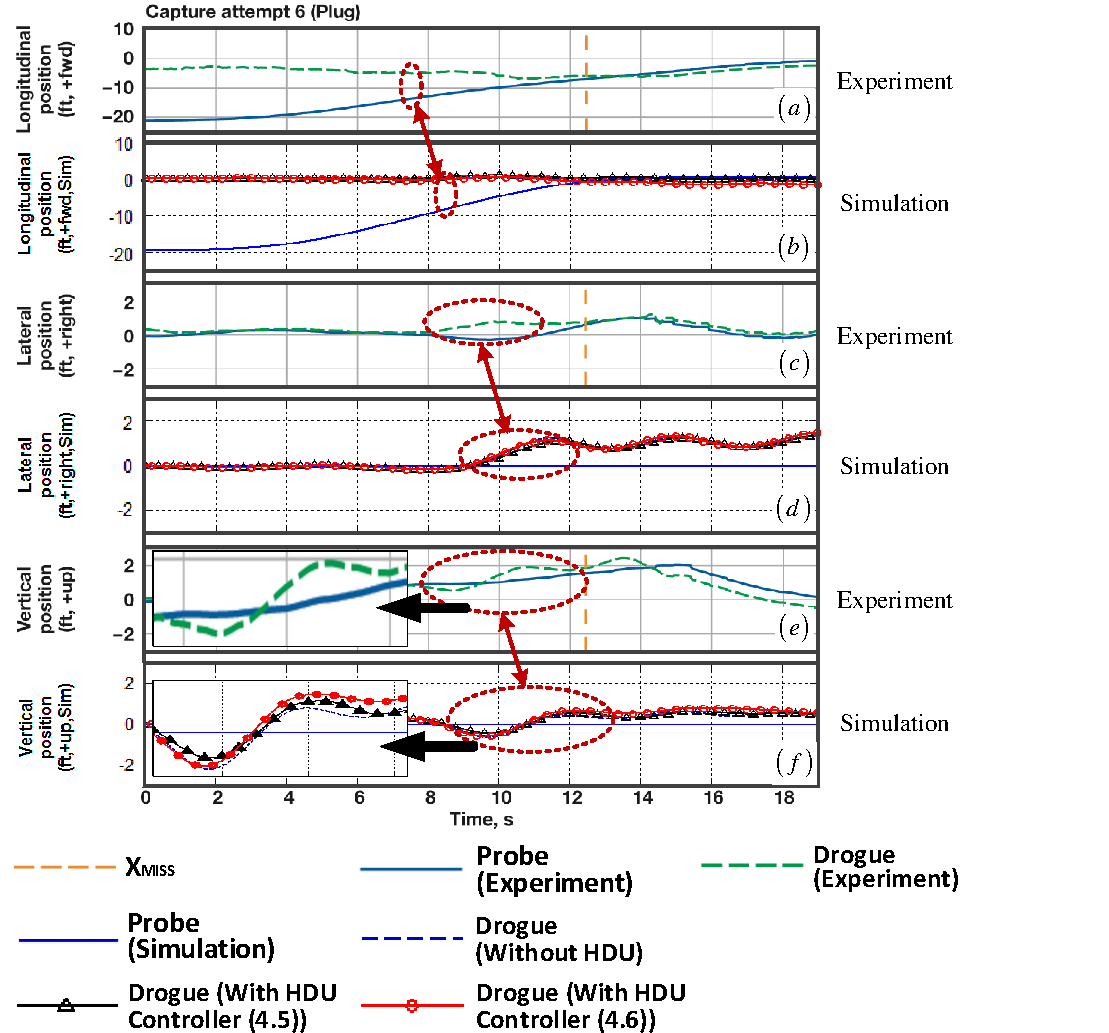
\includegraphics[width=0.7\textwidth]{Chap4/fig29.pdf}
%	\caption{Comparison of Drogue Dynamics during the Docking Process}\label{fig4.29}
%\end{figure} 
%Based on Fig. \ref{fig4.29}, the HDU has a slight influence on the drogue dynamics. However, during the docking process, even a small error of a few centimeters can lead to docking failure. Therefore, this influence remains significant. The two subplots Fig. \ref{fig4.29} (e) and (f) illustrate the differences in drogue dynamics in the vertical direction during docking, which is in accordance with the issue highlighted in the conclusions of Section 4.3.
%Additionally, from Fig. \ref{fig4.30}, it is even more evident that compared with the scenario without HDU, the vertical descent of the drogue with HDU is significantly reduced. In other words, the drogue dynamics considering the HDU model closely resemble the drogue dynamics observed in experiments.
%
%On the other hand, from Fig. \ref{fig4.29}, it is evident that the drogue dynamics under the control of the second type of controller differ from those without HDU and those under the control of the first type of controller. Although the swing amplitude of the drogue increases under the second type of controller, its adjustment speed is faster, which is more conducive to suppressing the hose whipping phenomenon. Furthermore, it can lead to a more accurate linearization of the model for the link-connected hose-drogue system with HDU. Therefore, it is still recommended to use the second type of controller for future HDU controller design.
%\begin{figure}[th]
%	\centering
%	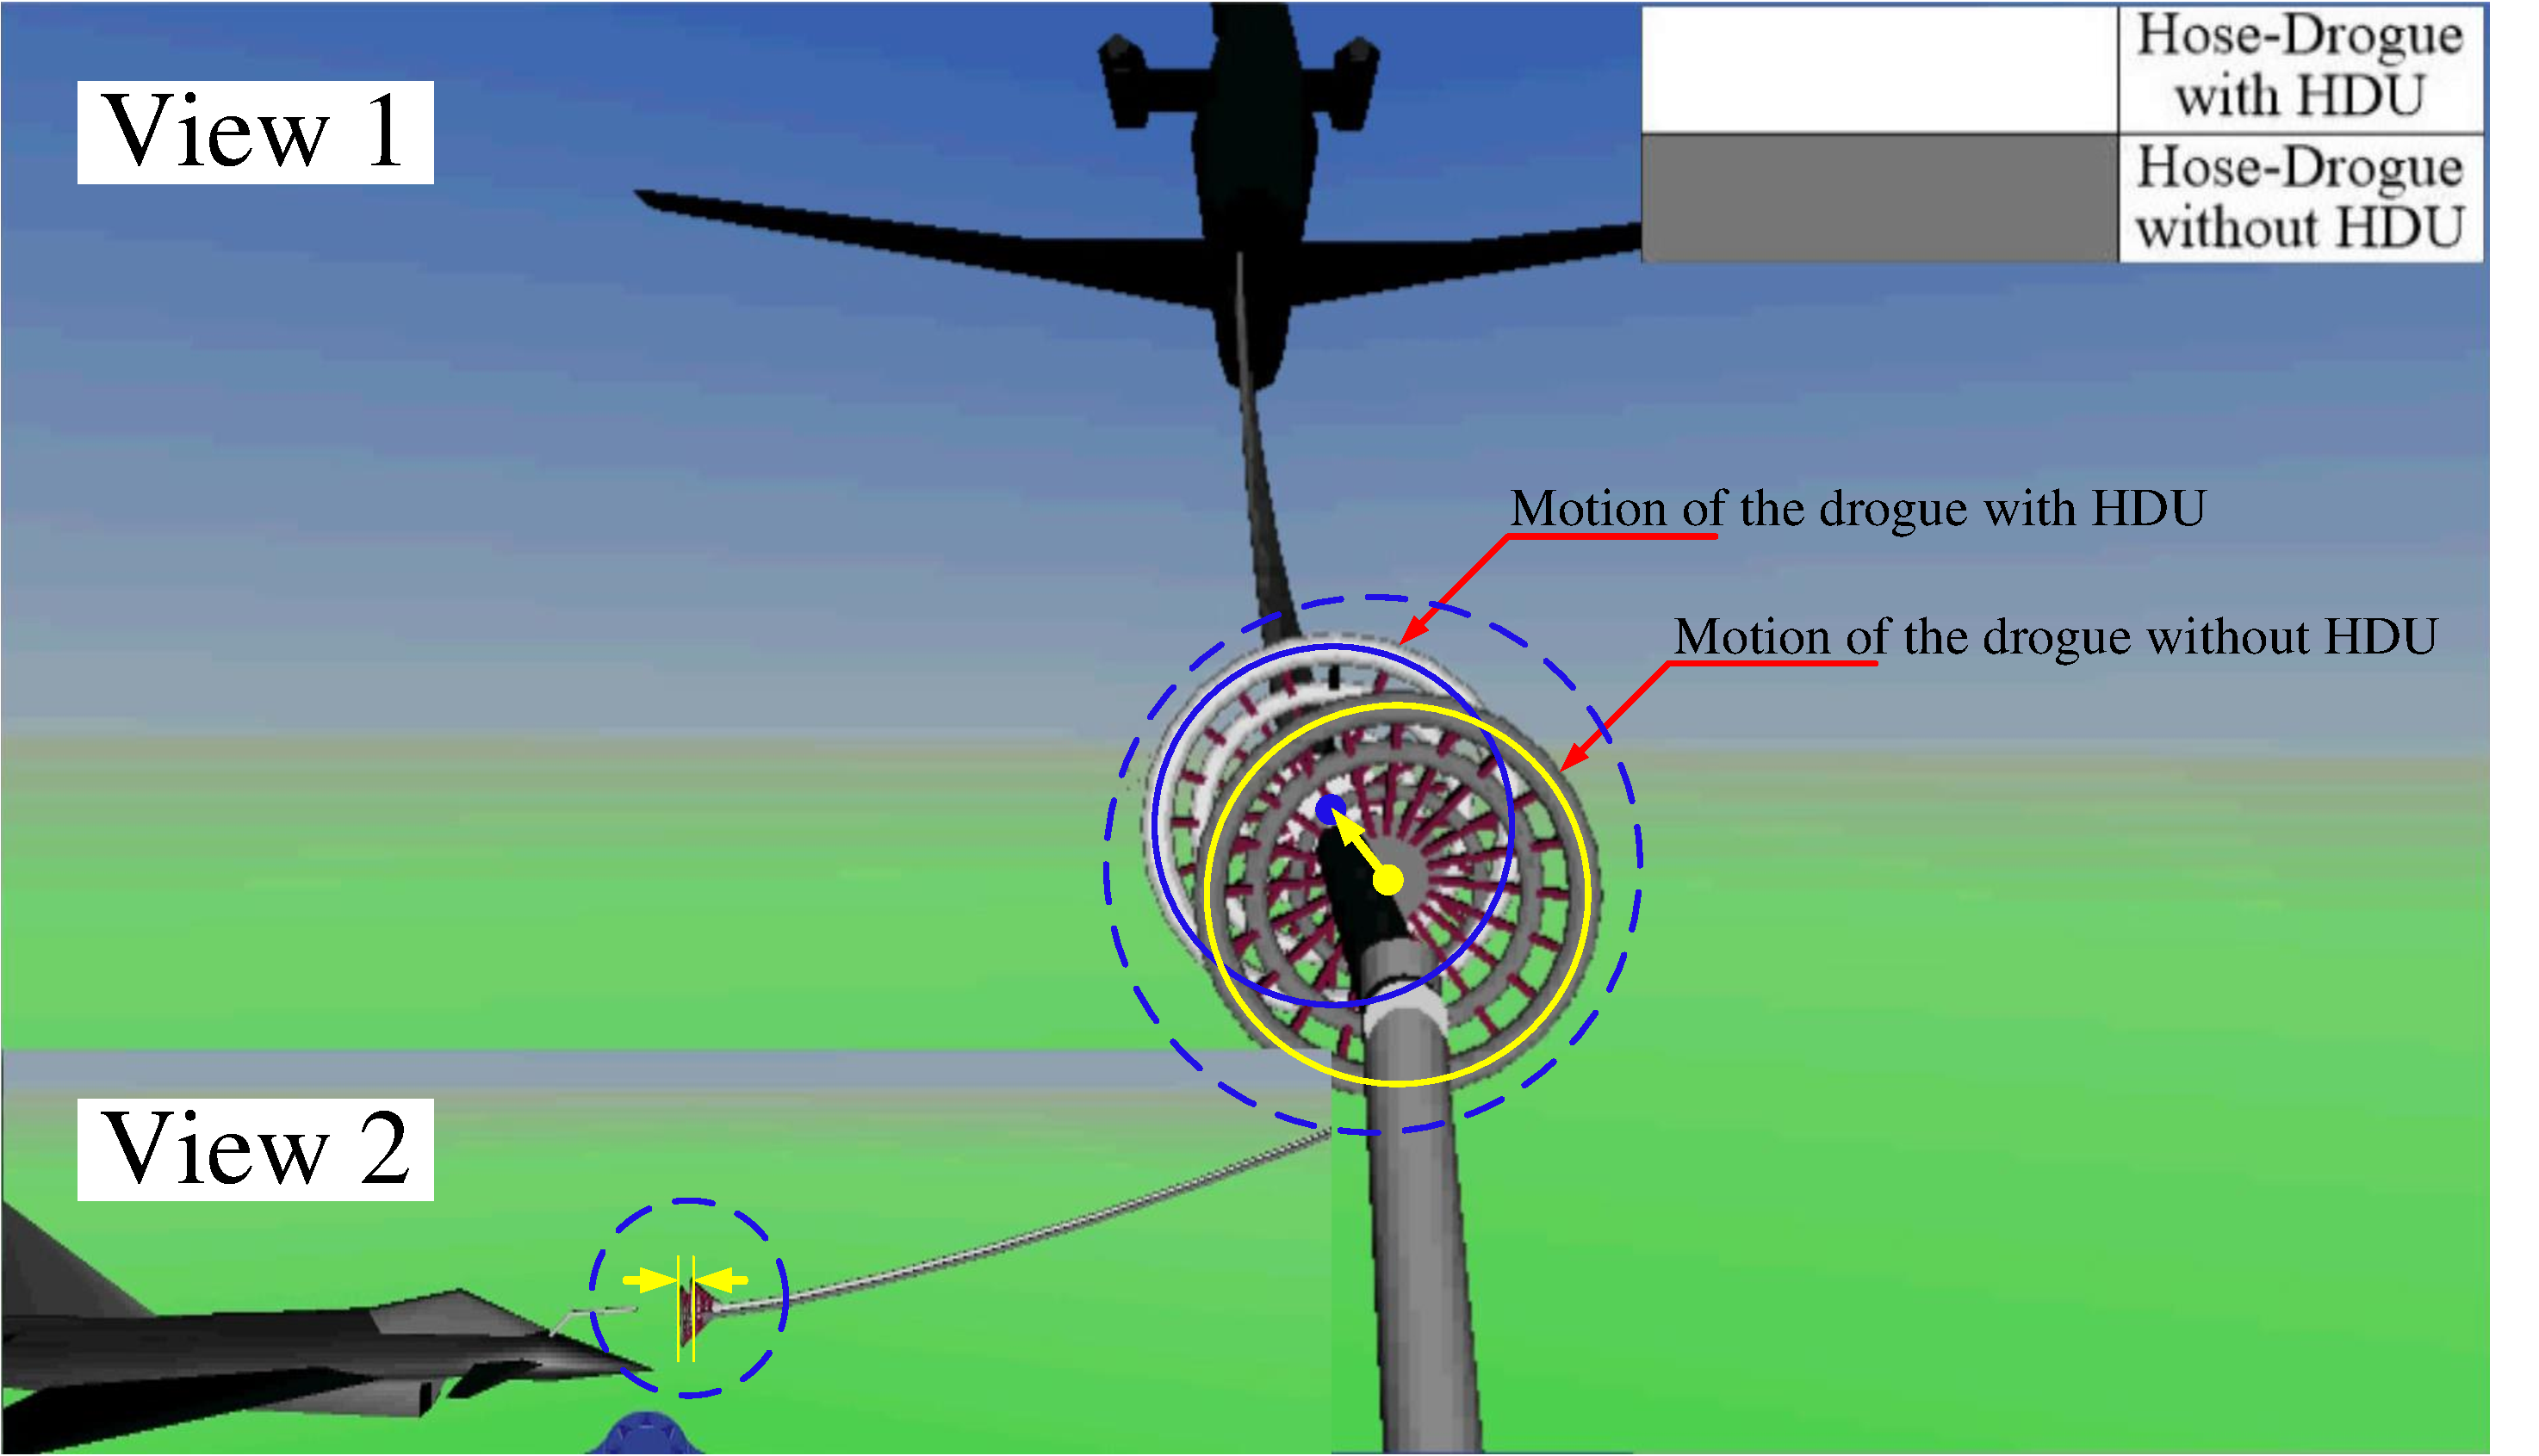
\includegraphics[width=0.7\textwidth]{Chap4/fig30.pdf}
%	\caption{Screenshot of the Simulation Video at Maximum Drogue Subsidence}\label{fig4.30}
%\end{figure} 


\chapter{Aerodynamic Disturbances}

The aerodynamic disturbances is one of the reasons why the aerial refueling mission is very difficult. The disturbances will act on the tanker and receiver aircraft to cause the aircraft away from the desired flight, and will also act on the hose and the drogue to cause the drogue to swing irregularly. In order to accurately simulate the environment of aerial refueling, the modeling of airflow disturbances is essential. Aerodynamic disturbances are multifaceted, including atmospheric turbulence, wake vortex of the tanker aircraft, wind gust and wind shear, ect. In general, non-uniform wind disturbances can be approximated by decomposing them into a uniform wind disturbance component and a uniform wind gradient component, namely, translational and rotational wind speeds. By decomposing the various wind disturbances into translational and rotational wind speeds and then superimposing them in each direction, the total wind disturbance is obtained. In this chapter, the various wind disturbances encountered during aerial refueling are analyzed in detail.

\section{Atmospheric Turbulence}
%\IEEEPARstart{Multicopters} are used in a wide range of applications, including structural inspection, parcel delivery, search rescue, geographic mapping, and passenger carrying \cite{2017Introduction}. However, the multicopter will inevitably generate vibration in practice \cite{maj2009novel,gwak2020sound}. The airframe is an assembly formed by bolting various parts together. Due to the looseness of the bolts, the stiffness of this airframe will become lower, which will cause low-frequency vibration. Air disturbances, such as atmospheric turbulence can generate nonuniform flow fields. The multicopter is affected by the disturbed forces and moments when the multicopter is involved in this nonuniform flow field. The unreasonable arrangement of sensors, flight control boards, GPS, and other modules on the airframe will easily cause the center of gravity to offset. This offset will bring additional disturbance force, which will cause the airframe to vibrate. The output signals of these sensors in turn contain vibration noise \cite{Miljkovic}.  These noise-containing signals are passed to the propulsion unit (composed of the propeller and motor) via designed control signals, which further amplify the amplitude of vibration. Moreover, due to manufacturing accuracy or installation errors, the mass center of  the propeller may not be collinear with the shaft \cite{ghalamchi2019real}. Therefore, the quadcopter produces strong disturbance torque due to the unbalanced propeller.  Because of the high-speed rotation of the propeller, the resulting centrifugal force also changes periodically.  Its period is proportional to that of the propeller. The disturbed torque by the centrifugal force will further affect the attitude dynamics and finally cause vibration \cite{niemiec2022relative}. Therefore, suppressing the disturbance torque caused by the unbalanced mass is one of main tasks in this chapter.
 Atmospheric turbulence, also known as turbulence, is irregular, three-dimensional small-scale motion in the atmosphere with randomness. Atmospheric turbulence is a particularly common class of atmospheric motion. In general, the atmospheric winds in nature, especially in the aircraft operating environment, are variable and basically have no specific pattern. Through a long period of observation and measurement of the wind field, meteorologists found that in a certain region and a certain period of time, the size of the wind speed always changes near a basic value. The basic value is defined as the average wind, and the fluctuations from the value is called turbulence. Atmospheric turbulence is generally considered to be a bounded random perturbation and is independent of the state of the tanker and the receiver aircraft. This disturbance occurs in all phases of aerial refueling.

The atmospheric turbulence model commonly used in aerospace is the Dryden model\cite{military1980u}, which uses a white noise signal of finite bandwidth and unit variance to generate the desired turbulence model output by passing it through a forming filter. The turbulence signal consists of three velocity components $u_{\mathrm{D}}^{\mathrm{b}}$, $v_{\mathrm{D}}^{\mathrm{b}}$, $w_{\mathrm{D}}^{\mathrm{b}}$ and three angular velocity components $p_{\mathrm{D}}^{\mathrm{b}}$, $q_{\mathrm{D}}^{\mathrm{b}}$, $r_{\mathrm{D}}^{\mathrm{b}}$, all of which are defined in the body coordinate system. For simplicity, the right superscript will be ignored in the following discussion, namely, the velocity component and the angular velocity component are expressed as $u_{\mathrm{D}}$, $v_{\mathrm{D}}$, $w_{\mathrm{D}}$ and $p_{\mathrm{D}}$, $q_{\mathrm{D}}$, $r_{\mathrm{D}}$. According to the U.S. Army military specification MILF\_8785C\cite{military1980u}\cite{chalk1969background}, the velocity and angular velocity spectral functions of the forming filter in the Dryden model are defined as follows\\
\begin{equation}\label{eq1}
\begin{aligned}
& \Phi_{u_D}(\omega)=\frac{2 \sigma_u^2 L_u}{\pi V_a} \cdot \frac{1}{1+\left(L_u \frac{\omega}{V_a}\right)^2} \quad \Phi_{p_D}(\omega)=\frac{\sigma_w^2}{V_a L_w} \cdot \frac{0.8\left(\frac{\pi L_w}{4 b}\right)^{1 / 3}}{1+\left(\frac{4 b \omega}{\pi V_a}\right)^2}\\ 
& \Phi_{v_D}(\omega)=\frac{\sigma_v^2 L_v}{\pi V_a} \cdot \frac{1+3\left(L_v \frac{\omega}{V_a}\right)^2}{\left[1+\left(L_v \frac{\omega}{V_a}\right)^2\right]^2} \quad \Phi_{r_D}(\omega)=\frac{\left(\frac{\omega}{V_a}\right)^2}{1+\left(\frac{3 b \omega}{\pi V_a}\right)^2} \cdot \Phi_{v_D}(\omega) \\
& \Phi_{w_D}(\omega)=\frac{\sigma_w^2 L_w}{\pi V_a} \cdot \frac{1+3\left(L_w \frac{\omega}{V_a}\right)^2}{\left[1+\left(L_w \frac{\omega}{V_a}\right)^2\right]^2} \quad \Phi_{q_D}(\omega)=\frac{\left(\frac{\omega}{V_a}\right)^2}{1+\left(\frac{4 b \omega}{\pi V_a}\right)^2} \cdot \Phi_{w_D}(\omega) \\
%&
\end{aligned}
\end{equation}
where $b$ denotes aircraft wingspan, $V_a$ denotes the airspeed, $L_u$, $L_v$, $L_w$ denote the turbulence scale, and $\sigma_u$, $\sigma_v$, $\sigma_w$ denote the turbulence intensity, which have different values at different altitudes. Specifically, when the altitude is less than 1000 ft. the model is called the low altitude model and the values of the parameters are
\begin{equation}\label{eq2}
L_w=h, \quad L_u=L_v=\frac{h}{(0.177+0.000823 h)^{1.2}}
\end{equation}
where $h$ is in feet. In particular, when the altitude is 20 feet (about 6 metres), a wind speed of 15 knots (about 7.7 m/s) is a mild turbulence, a wind speed of 30 knots is a moderate turbulence, and a wind speed of 45 knots is a severe turbulence. Using $W_{20}$ to represent the wind speed at 20 feet above sea level, the turbulence intensity satisfies the
\begin{equation}\label{eq3}
\sigma_w=0.1 W_{20}, \quad \frac{\sigma_u}{\sigma_w}=\frac{\sigma_v}{\sigma_w}=\frac{1}{(0.177+0.000823 h)^{0.4}}
\end{equation}
When the altitude is greater than 2,000 ft, it is called a medium to high altitude model, and under the assumption of isotropy, there are
\begin{equation}\label{eq4}
L_u=L_v=L_w, \quad \sigma_u=\sigma_v=\sigma_w
\end{equation}
Specific values can refer to literature\cite{military1980u}. Besides, one can directly use the corresponding modules in Simulink's Aerospace toolbox. When the altitude is between 1000 and 2000 ft, the turbulent velocity and the turbulent angular velocity can be obtained from by linear interpolation of the values taken at 1000 ft for the low altitude model and 2000 ft for the medium and high altitude model. It should be noted that in the low altitude model, the direction of the turbulent velocity is slightly different from the direction of the ground coordinate system. Specifically, the turbulent velocity component is oriented in the horizontal plane and in the same direction as the mean wind vector.

Based on the spectral square root of the spectral function, the transfer function of the forming filter can be obtained as follows

\begin{equation}\label{eq5}
\begin{aligned}
& H_{u_D}(s)=\sigma_u \sqrt{\frac{2 L_{u l}}{\pi V_a}} \cdot \frac{1}{1+\frac{L_{u l}}{V_a} s} \quad H_{p_D}(s)=\sigma_w \sqrt{\frac{0.8}{V_a}} \cdot \frac{\left(\frac{\pi}{4 b}\right)^{1 / 6}}{L_w^{1 / 3}\left(1+\left(\frac{4 b}{\pi V_a}\right) s\right)} \\
& H_{v_D}(s)=\sigma_v \sqrt{\frac{L_v}{\pi V_a}} \cdot \frac{1+\frac{\sqrt{3} L_v}{V_a} s}{\left(1+\frac{L_v}{V_a} s\right)^2} \quad H_{r_D}(s)=\frac{\frac{s}{V_a}}{1+\left(\frac{3 b}{\pi V_a}\right) s} \cdot H_{v_D}(s) \\
& H_{w_D}(s)=\sigma_w \sqrt{\frac{L_w}{\pi V_a}} \cdot \frac{1+\frac{\sqrt{3} L_w}{V_a} s}{\left(1+\frac{L_w}{V_a} s\right)^2} \quad H_{q_D}(s)=\frac{\frac{s}{V_a}}{1+\left(\frac{4 b}{\pi V_a}\right) s} \cdot H_{w_D}(s) \\
%&
\end{aligned}
\end{equation}\\
Therefore, by passing the white noise signal with unit variance through this forming filter, the turbulence signal containing three velocity components and three angular velocity components can be obtained.

\section{Wind Gust Model}
A gust, also known as a sudden gust, is a sudden change in wind speed that occurs over a short period of time. The uncertainty of atmospheric motion causes the speed and direction of gusts to change rapidly all the time. It is generally accepted that gusts, like atmospheric turbulence, are bounded random disturbances and are independent of the state of the tanker and the receiver aircraft. This disturbance occurs in all phases of aerial refueling.

A widely used model is the 1-cosine discrete gust model, the shape of which is shown in Fig. \ref{fig1}. In this model,
\begin{figure}[th]
	\centering
	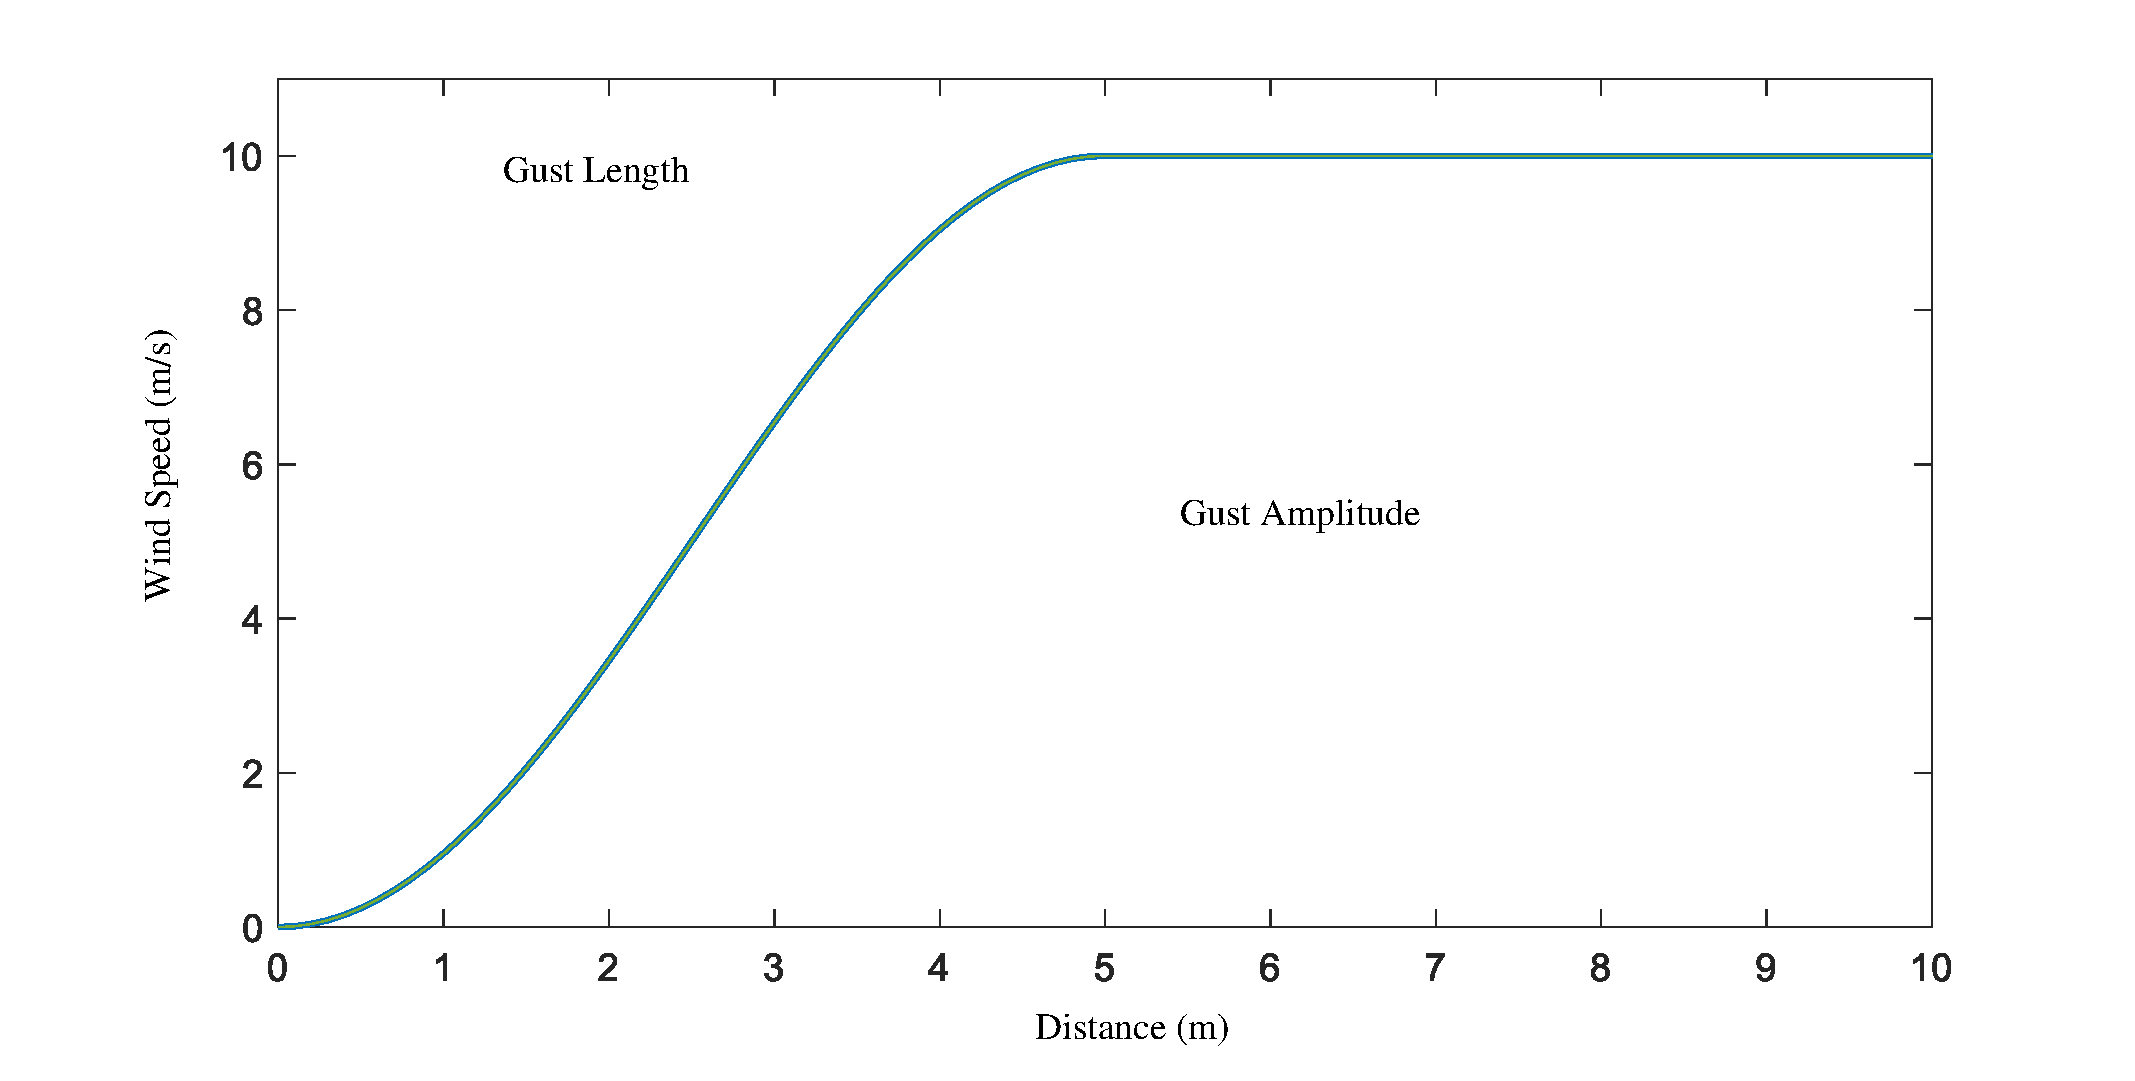
\includegraphics[width=0.8\textwidth]{Figures/Figs_Ch4/fig1.pdf}
	\caption{Half-wavelength atmospheric disturbance gust modelling\cite{ly1980time}}\label{fig1}
\end{figure}\\
the gust contains three velocity components $u_{\mathrm{G}}^{\mathrm{b}}$, $v_{\mathrm{G}}^{\mathrm{b}}$ and $w_{\mathrm{G}}^{\mathrm{b}}$ in the body coordinate system and the three velocities are uncorrelated and have the same mathematical model. The 1-cosine discrete gust model is available in both full-wavelength and half-wavelength model. Taking the velocity $u_{\mathrm{G}}^{\mathrm{b}}$ in the direction of the body axis $o_{\mathrm{b}}x_{\mathrm{b}}$ as an example, the full-wavelength 1-cosine discrete gust model is

\begin{equation}\label{eq6}
u_{\mathrm{G}}^{\mathrm{b}}(x)= \begin{cases}0 & x<0 \\ \frac{V_m}{2}\left(1-\cos \left(\frac{\pi x}{d_m}\right)\right) & 0<x<2 d_m \\ 0 & x>2 d_m\end{cases}
\end{equation}
and the half-wavelength 1-cosine discrete gust model is
\begin{equation}
u_{\mathrm{G}}^{\mathrm{b}}(x)= \begin{cases}0 & x<0 \\ \frac{V_m}{2}\left(1-\cos \left(\frac{\pi x}{d_m}\right)\right) & 0<x<d_m \\ V_m & x>d_m\end{cases}
\end{equation}
where $V_m$ denotes the gust intensity, namely, the maximum value of gust wind speed; $d_m$ denotes the gust scale, namely, the transition distance of gust establishment; $x$ denotes the distance into the gust. By applying the gust model to the three body axes of the aircraft, $u_{\mathrm{G}}^{\mathrm{b}}(x)$, $v_{\mathrm{G}}^{\mathrm{b}}(x)$ and $w_{\mathrm{G}}^{\mathrm{b}}(x)$ can be obtained.

Before the 1980s, the full-wavelength 1-cosine discrete gust model was more often used. With the continuous improvement of numerical simulation technology, the traditional full-wavelength model can no longer satisfy the needs of the study. After the 1980s, the half-wavelength 1-cosine discrete gust model is more often used. Compared with the full-wavelength 1-cosine discrete gust model, the half-wavelength 1-cosine discrete gust model is more convenient and flexible. The half-wavelength 1-cosine discrete gust model is used in the U.S. military specification MIL-F-8785C\cite{military1980u} and has been modularised in Simulink's Aerospace toolbox.

\section{Wind Shear}
Wind shear refers to the sudden change of wind direction or wind speed between any two points in space within a certain period of time, including the sudden vertical shear of horizontal winds, the horizontal shear of horizontal winds and the shear of vertical winds. Research results show that wind shear often occurs in the low and medium-altitude areas where aircraft take off and land, posing a great danger and threat to the safe operation of aircraft.

At present, there are three main ways of modeling wind shear. The first way is to store the Doppler radar measurement data in the form of a grid in the computer, and it is also possible to establish a wind shear incident database. The data is real and the amount of data storage depends on the division of the grid size, and the interpolation method can be adopted to take the values in use. However, the cost required by this method is very high; the second way is to establish and numerically solve the atmospheric dynamics equations in accordance with the laws of hydrodynamics and thermodynamics. The equations of atmospheric dynamics are nonlinearly differential and it generally takes up a lot of memory and machine time to solve to equations numerically. The real-time performance of this method is generally difficult to meet, and it is not suitable for engineering simulation; the third way is to establish an engineering simulation model, that is, to establish a relatively simplified mathematical model that describes the nature of the wind shear phenomenon, the mechanism and the movement process. This engineering wind shear model is simple and flexible, easy to use, and has better realism, so it is more suitable for atmospheric wind field simulation applications\cite{noauthor__nodate}.

The most widely used models for wind shear in the ground boundary layer are the logarithmic and exponential models. The Prandtl logarithmic model is expressed as
\begin{equation}\label{eq8}
u_{\mathrm{S}}(h)=\frac{u_{\mathrm{S} 0}}{k} \ln \frac{h}{h_0}
\end{equation}
where $h$ is the altitude; $u_{\mathrm{S0}}$ is the friction velocity, which depends on the shear stress on the ground $\tau_0$ and the air density $\rho_0$, denoted as $u_{\mathrm{S0}}=\sqrt{\tau_0/\rho_0}$; $h_0$ characterises the effect of the roughness of the ground; and $k=0.4$ is known as Karman's constant.

The exponential model for wind shear in the ground boundary layer takes the form
\begin{equation}\label{eq9}
u_{\mathrm{S}}(h)=u_{\mathrm{SR}}\left(\frac{h}{h_R}\right)^m
\end{equation}
where $h$ is the altitude; $u_{\mathrm{SR}}$ is the mean wind speed at the reference altitude $h_R$; and $m$ is the wind shear index, which is affected by factors such as ground roughness $h_0$ and temperature gradient ${dT/dh}$ \cite{gipe1993wind}.

In the U.S. Army military specification MIL-F-8785C\cite{military1980u}, the logarithmic model used for horizontal wind variation with height is
\begin{equation}\label{eq10}
u_{\mathrm{S}}(h)=W_{20} \frac{\ln \left(\frac{h}{z_0}\right)}{\ln \left(\frac{20}{z_0}\right)}, \quad 3 f t<h<1000 {ft}
\end{equation}
where $h$ is the altitude; $W_{20}$ denotes the wind speed at 20 ft above sea level; and $z_0$ takes the value of 0.15 ft for the Class $\mathbf{C}$ phase of flight (specifically defined in the literature \cite{military1980u}, which generally refers to the take-off and landing phases), and $z_{0}$ takes the value of 2.0 ft for the other phases.

It is worth noting that the wind shear velocity derived from the above model is the horizontal mean wind velocity, which can be projected in the ground coordinate system if the angle between the wind direction and the earth's axis is known. In particular, assuming that the angle between the direction of the wind and the earth's axis $o_{\mathrm{g}}x_{\mathrm{g}}$ is $\theta_{\mathrm{S}}$, the velocity component of the wind shear in the ground coordinate system is expressed as follows
\begin{equation}\label{eq11}
\mathbf{v}_{\mathrm{S}}^\mathrm{g}(h)=\left[\begin{array}{c}
u_{\mathrm{S}}^\mathrm{g}(h) \\
v_{\mathrm{S}}^\mathrm{g}(h) \\
w_{\mathrm{S}}^\mathrm{g}(h)
\end{array}\right]=\left[\begin{array}{c}
u_{\mathrm{S}}(h) \cos \theta_{\mathrm{S}} \\
u_{\mathrm{S}}(h) \sin \theta_{\mathrm{S}} \\
0
\end{array}\right]
\end{equation}
It should be noted that $h$ is the altitude, which is satisfied by $z_\mathrm{g}=-h$ in the ground coordinate system. This can then be transformed to the aircraft body coordinate system by means of the coordinate system transformation method
\begin{equation}\label{eq12}
\mathbf{v}_{\mathrm{S}}^{\mathrm{b}}(h)=\left[\begin{array}{c}
u_{\mathrm{S}}^{\mathrm{b}}(h) \\
v_{\mathrm{S}}^{\mathrm{b}}(h) \\
w_{\mathrm{S}}^{\mathrm{b}}(h)
\end{array}\right]=\mathbf{R}_{\mathrm{b} / \mathrm{g}}(\theta, \psi, \phi) \mathbf{v}_{\mathrm{S}}^{\mathrm{g}}(h)
\end{equation}
where $u_{\mathrm{S}}^{\mathrm{b}}(h)$, $v_{\mathrm{S}}^{\mathrm{b}}(h)$ and $w_{\mathrm{S}}^{\mathrm{b}}(h)$ are the three components of the induced velocity from wind shear on the aircraft body axis.

\section{Tanker Wake}
Tanker wake vortex is a kind of perturbation due to the presence of pressure differences between the upper and lower surfaces of the tanker wing, the airflow on the lower wing surface is reversed upwards around the wing tip under the effect of pressure difference to form a vortex spreading backward, thus affecting the receiver aircraft. It belongs to  non-random perturbations, related to the state of the tanker but not related to the state of the receiver. The perturbation occurs in the last four phases when the tanker and receiver aircraft are close to each other, and it can be equated to a constant angle of attack perturbation due to the small change in the relative positions of the tanker and the receiver aircraft in the docking phase.

According to the lift line theory\cite{pamadi2004performance}. Vortices from the wing and horizontal tail of a tanker can be modeled as horseshoe Vortices as shown in Fig. \ref{fig2}. Four vortex lines along the axis of the airflow coordinate system $o_{\mathrm{w}}x_{\mathrm{w}}$ are trailed by the wing tip and tail tip, which correspond to vortex line \ding{172}\ding{173}\ding{174}\ding{175} in Fig. \ref{fig2}; and two vortex lines exist in the direction of the wingspan and the tail, which correspond to vortex line \ding{176} and \ding{177} in Fig. \ref{fig2}, respectively. When the wing generates positive lift, the wing tip vortex rotates inward; when the horizontal tail generates negative lift, the tail tip vortex rotates outward. Thus, the vortices on the wing and tail are in opposite directions. Since the lift generated by the wing is much greater than that generated by the tail, the wing vortices are much stronger than the tail vortices.
\begin{figure}[th]
	\centering
	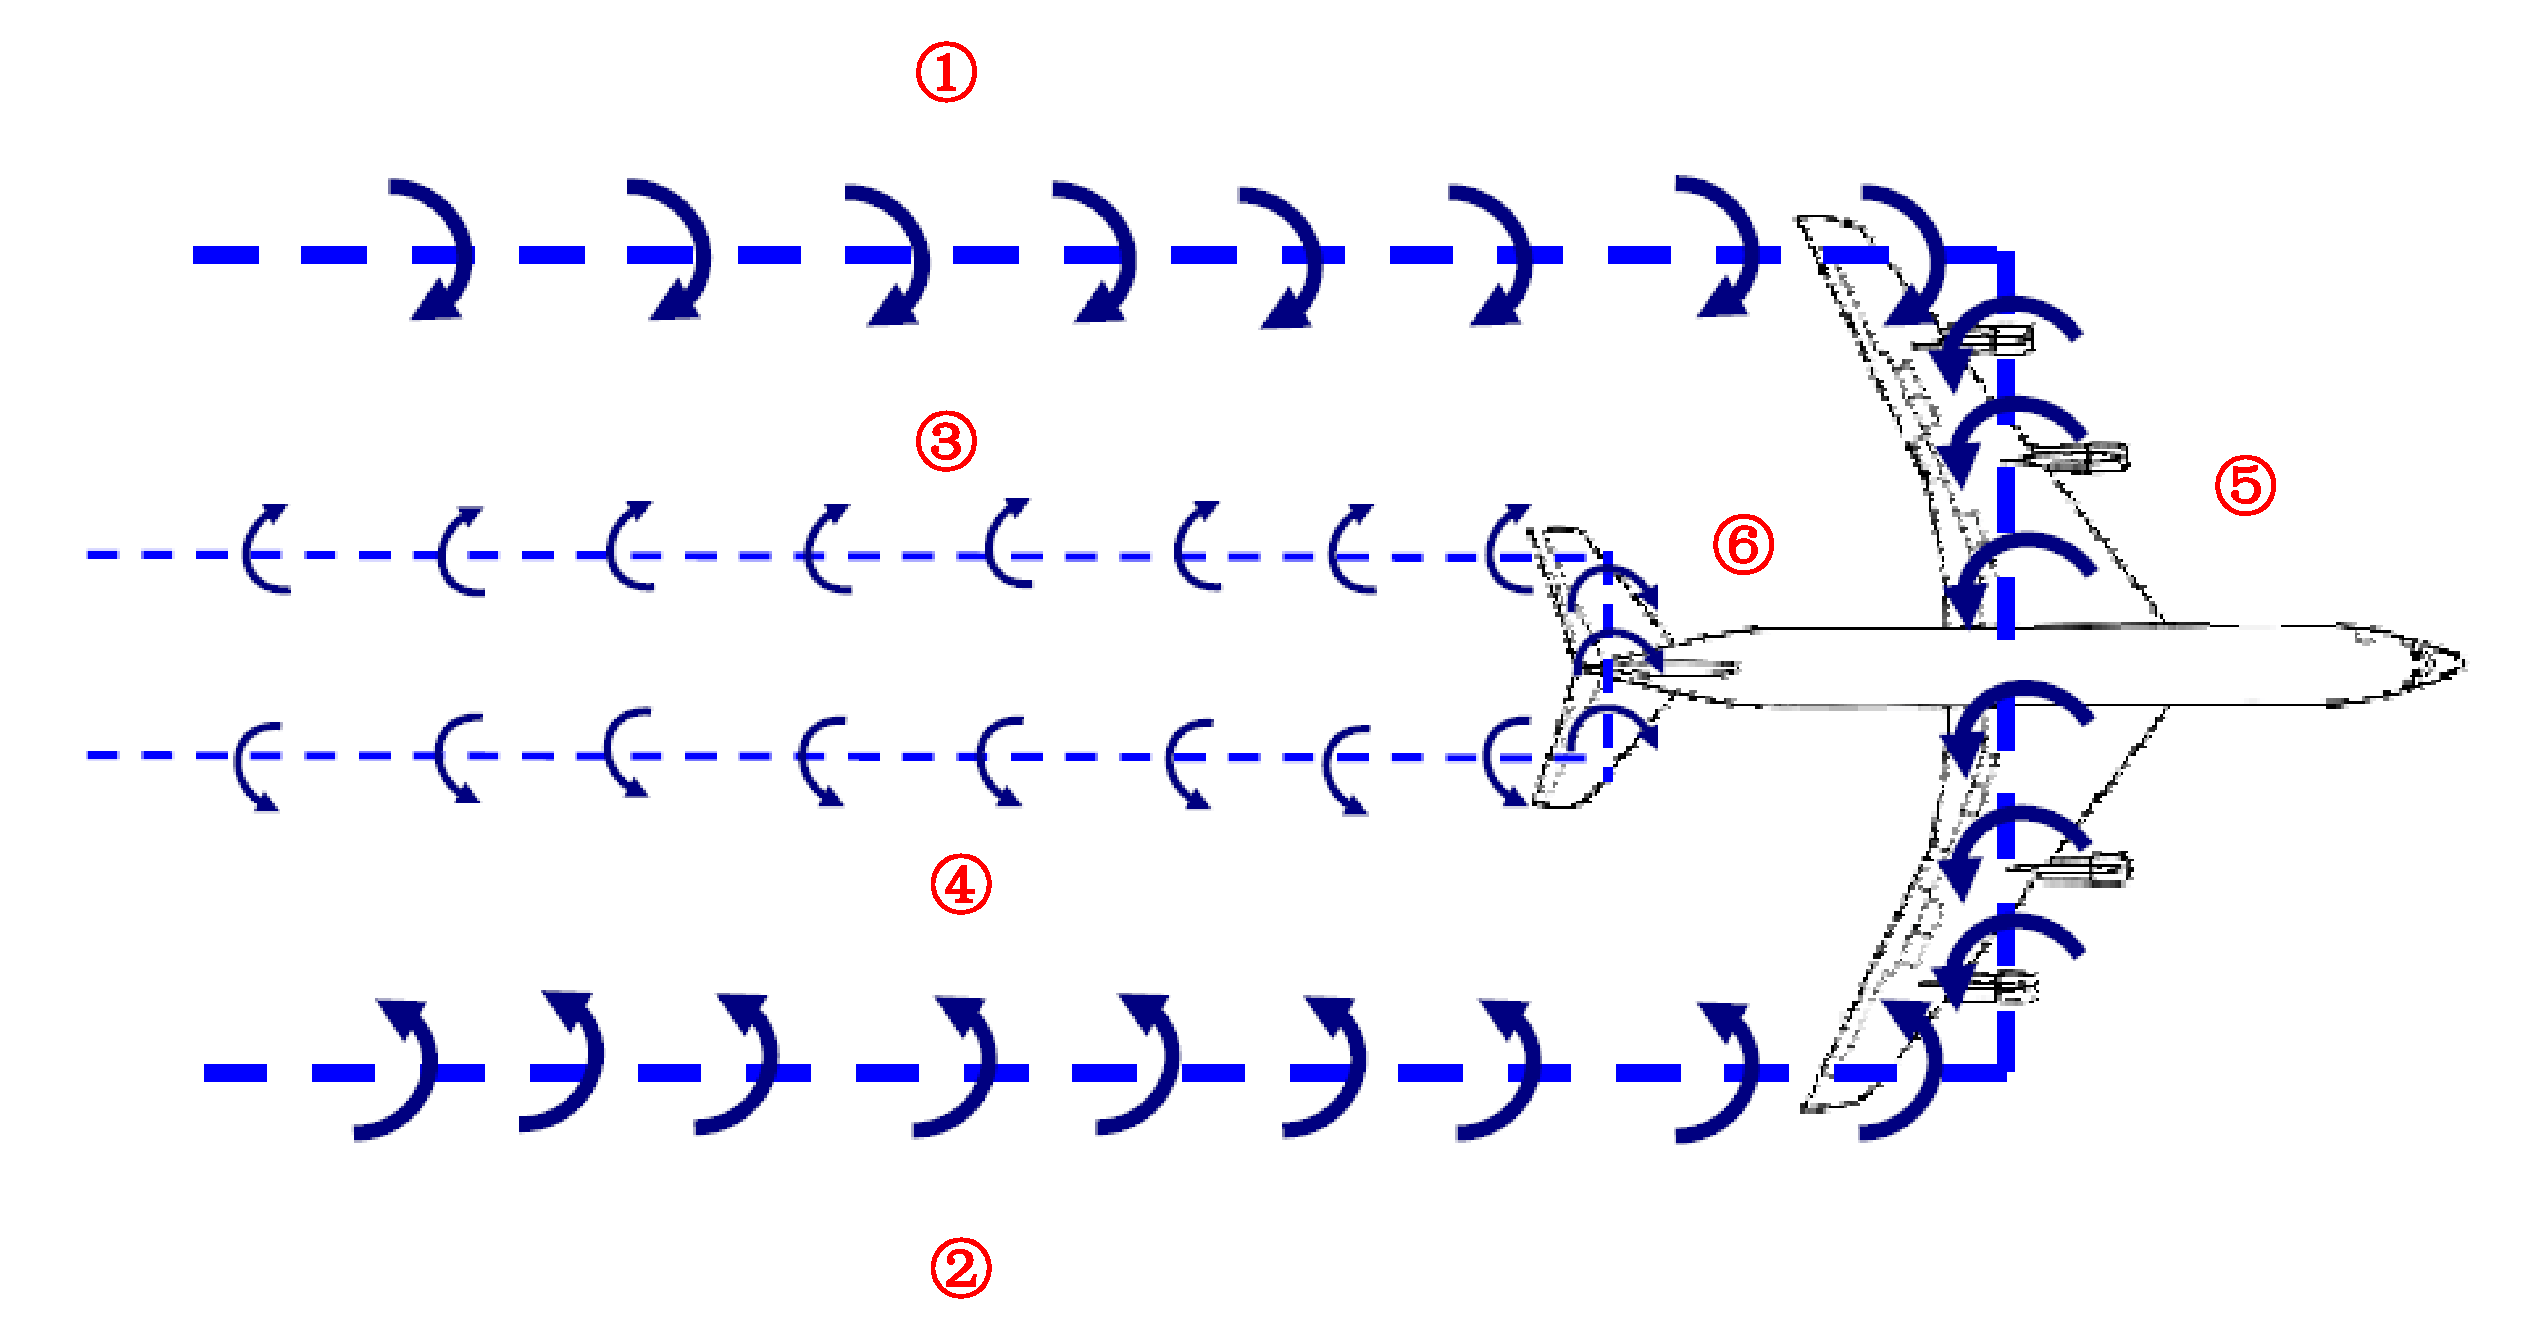
\includegraphics[width=0.9\textwidth]{Figures/Figs_Ch4/fig2.pdf}
	\caption{Schematic of the wing and horizontal tail saddle vortex\cite{pamadi2004performance}}\label{fig2}
\end{figure}

For simplicity of analysis, wingtip vortices are generally considered to be a series of circular swirling motions with the center of the circle located on the vortex line, producing induced velocities tangent to the circle. For any position in the near airspace of the tanker, it is simultaneously affected by the six vortices in Fig. \ref{fig2}. By analyzing the effect of each vortex separately and then superimposing them the total effect of the tanker wake on any position in the space can be obtained. As shown in Fig. \ref{fig3}, assuming that in the airflow coordinate system, the relative position coordinate of any point $\text{p}$ in space relative to the center of the wingtip vortex $\text{o}$ is $\mathbf{p}_{{\mathrm{p} \mathrm{\left/{\vphantom {p o}} \right.\kern-\nulldelimiterspace}\mathrm {o}}}^{\mathrm{w}} = {\left[ {\begin{array}{*{20}{c}}{x_{{\mathrm{p} \mathrm{\left/{\vphantom {p o}} \right.\kern-\nulldelimiterspace}\mathrm{o}}}^{\mathrm{w}}}&{y_{{\mathrm{p} \mathrm{\left/{\vphantom {p o}} \right.\kern-\nulldelimiterspace} \mathrm{o}}}^{\mathrm{w}}}&{z_{{\mathrm{p} \mathrm{\left/{\vphantom {p o}} \right.\kern-\nulldelimiterspace}\mathrm{o}}}^{\mathrm{w}}}\end{array}} \right]^\mathrm{T}}$; $r_{R} = \left\| {\mathbf{p}_{{\mathrm{p} \mathrm{\left/{\vphantom {p o}} \right.\kern-\nulldelimiterspace} \mathrm{o}}}^{\mathrm{w}}} \right\|$ is the radial distance from the position $\mathbf{p}$ to the vortex line; the induced velocity of the left wingtip vortex at the point $\mathbf{p}$ is $\mathbf{v}_{\mathrm{LWI}}^\mathrm{w}$, and the direction is tangent to the circular vortex; and the angle of induced velocity $\mathbf{v}_{\mathrm{LWI}}^\mathrm{w}$ and the axis of $o_{\mathrm{w}}y_{\mathrm{w}}$ in the airflow coordinate system is ${\theta _\mathrm{LWI}}$.
\begin{figure}[th]
	\centering
	\includegraphics[width=0.6\textwidth]{Figures/Figs_Ch4/fig3.pdf}
	\caption{Schematic diagram of a tanker wake}\label{fig3}
\end{figure}

According to literature\cite{dogan2008flight}, the size of the induced velocity produced by each vortex line at the point $\mathbf{p}$ is
\begin{equation}\label{eq13}
V=\frac{\Gamma r_R}{2 \pi\left(r_R^2+r_c^2\right)}\left(1-\exp \left(-\frac{r_R^2}{4 v \tau}\right)\right)
\end{equation}
where $\Gamma$ is the vortex strength, $r_c$ is the radius of the vortex core which can be taken as $r_c=2.24\sqrt{\upsilon\tau}$, $\upsilon$ is the viscosity coefficient which can be taken as $\upsilon=0.06\times\Gamma$, $\tau$ is the vortex time coefficient related to the airspeed of the tanker,  $r_{R} = \left\| {\mathbf{p}_{{\mathrm{p} \mathrm{\left/{\vphantom {p o}} \right.\kern-\nulldelimiterspace} \mathrm{o}}}^{\mathrm{w}}} \right\|$ is the radial distance from the position $\mathbf{p}$ to the vortex line.

The vortex strength can be calculated by the following equation as follows 
\begin{equation}\label{eq14}
\Gamma=\frac{L}{\rho V_t(\pi / 4) b} \frac{\cos \gamma_1+\cos \gamma_2}{2}
\end{equation}
where $b$ is the wingspan of the tanker, $\rho$ is the air density, $V_t$ is the airspeed of the tanker, and $L$ is the lift generated by the wings or tail of the tanker; $\gamma_1$ and $\gamma_2$ is the angle from the end point of the vortex line to the current point. For bound vortices, namely, vortex lines \ding{176}\ding{177} in Fig. \ref{fig2}, both $\gamma_1$ and $\gamma_2$ are non-zero; for tip vortices, namely, vortex lines \ding{172}\ding{173}\ding{174}\ding{175} in Fig. \ref{fig2}, $\gamma_1$ and $\gamma_2$ are equal to zero.

According to Eqs. (\ref{eq13}) and (\ref{eq14}), the induced velocities of the six vortices generated at any point $\mathbf{p}$ in the space can be calculated, including left wingtip vortex $\mathbf{v}^\mathrm{w}_\mathrm{LWV}$, right wingtip vortex $\mathbf{v}^\mathrm{w}_\mathrm{RWV}$, left tailtip vortex $\mathbf{v}^\mathrm{w}_\mathrm{LTV}$, right tailtip vortex $\mathbf{v}^\mathrm{w}_\mathrm{RTV}$, wing spreading vortex $\mathbf{v}^\mathrm{w}_\mathrm{WV}$ and horizontal tail spreading vortex $\mathbf{v}^\mathrm{w}_\mathrm{TV}$, respectively. The components of $\mathbf{v}^\mathrm{w}_\mathrm{LWV}$, $\mathbf{v}^\mathrm{w}_\mathrm{RWV}$, $\mathbf{v}^\mathrm{w}_\mathrm{LTV}$ and $\mathbf{v}^\mathrm{w}_\mathrm{RTV}$ lie in the plane of the airflow coordinate system ${o}_\mathrm{w}{y}_\mathrm{w}{z}_\mathrm{w}$ and therefore have a component of 0 along the $o_\mathrm{w}x_\mathrm{w}$ axis, while $\mathbf{v}_\mathrm{WI}^\mathrm{w}$ and $\mathbf{v}_\mathrm{TV}^\mathrm{w}$ lie in the plane of the airflow coordinate system ${o}_\mathrm{w}{x}_\mathrm{w}{z}_\mathrm{w}$ and therefore have a component of 0 along the ${o}_\mathrm{w}{y}_\mathrm{w}$ axis. Taking the induced velocity $\mathbf{v}^\mathrm{w}_\mathrm{LWV}$ generated by the left wingtip vortex in Fig. \ref{fig3} as an example, its component in the airflow coordinate system can be expressed as
\begin{equation}\label{eq15}
\mathbf{v}_{\mathrm{LWV}}^{\mathrm{w}}=\left[\begin{array}{c}
0 \\
-V_{\mathrm{LWV}} \cos \theta_{\mathrm{LWV}} \\
V_{\mathrm{LWV}} \sin \theta_{\mathrm{LWV}}
\end{array}\right]
\end{equation}
where $V_\mathrm{LWV}$ is the magnitude of the induced velocity generated by the left wingtip vortex, which can be calculated according to Eq. (\ref{eq13}). All other induced velocities can be decomposed into the airflow coordinate system. Specifically, in the aerial refueling process, the point $\mathbf{p}$ is the position of the receiver aircraft, and the direction of induced speed can be determined according to the relative position relationship between the receiver and the tanker.

The total induced velocity $\mathbf{v}^\mathrm{w}_\mathrm{V}$ generated by the tanker wake at any point in space can be obtained by summing the induced velocity generated by the six eddies at that point, which is expressed as follows
\begin{equation}\label{eq16}
\mathbf{v}_{\mathrm{V}}^{\mathrm{w}}(x, y, z)=\mathbf{v}_{\mathrm{LWV}}^{\mathrm{w}}+\mathbf{v}_{\mathrm{RWV}}^{\mathrm{w}}+\mathbf{v}_{\mathrm{LTV}}^{\mathrm{w}}+\mathbf{v}_{\mathrm{RTV}}^{\mathrm{w}}+\mathbf{v}_{\mathrm{WV}}^{\mathrm{w}}+\mathbf{v}_{\mathrm{TV}}^{\mathrm{w}}
\end{equation}
from the analysis, it can be seen that the induced speed generated by the tanker wake is a function of position. The total induced velocity $\mathbf{v}^\mathrm{w}_\mathrm{V}$ is decomposed into three components along the axial direction in the airflow coordinate system
\begin{equation}\label{eq17}
\mathbf{v}_{\mathrm{V}}^{\mathrm{w}}(x, y, z)=\left[\begin{array}{lll}
u_{\mathrm{V}}^{\mathrm{w}} & v_{\mathrm{V}}^{\mathrm{w}} & w_{\mathrm{V}}^{\mathrm{w}}
\end{array}\right]^{\mathrm{T}}
\end{equation}
According to the coordinate system conversion method introduced in chapter 2, the total induced velocity $\mathbf{v}^\mathrm{w}_\mathrm{V}$ in the airflow coordinate system can be transformed into the receiver aircraft body coordinate system. In the receiver aircraft body coordinate system, Eq. (\ref{eq16}) can be rewritten as 
\begin{equation}\label{eq18}
\mathbf{v}_{\mathrm{V}}^{\mathrm{r}}(x, y, z)=\mathbf{R}_{\mathrm{r} / \mathrm{w}}(\alpha, \beta) \mathbf{v}_{\mathrm{V}}^{\mathrm{w}}(x, y, z)=\left[\begin{array}{lll}
u_{\mathrm{V}}^{\mathrm{r}} & v_{\mathrm{V}}^{\mathrm{r}} & w_{\mathrm{V}}^{\mathrm{r}}
\end{array}\right]^{\mathrm{T}}
\end{equation}
where $\mathbf{R}_\mathrm{r / w}(\alpha, \beta)$=$\mathbf{R}_\mathrm{b / w}(\alpha,\beta)$, $\alpha$ and $\beta$ are the angle of attack and side slip angle of the receiver, respectively, and the velocity components $u^\mathrm{r}_\mathrm{V}$, $v^\mathrm{r}_\mathrm{V}$ and $w^\mathrm{r}_\mathrm{V}$ are all functions of position.

Based on the literature\cite{pamadi2004performance}, the non-uniform wind field can be approximately decomposed into a uniform wind disturbance component and a uniform wind gradient component, namely, translational wind speed and rotating wind speed. Therefore, the induced angular velocity $\boldsymbol{\omega}_\mathrm{V}^\mathrm{r}\left( {x,y,z} \right) = {\left[ {\begin{array}{*{20}{c}}
		{p_\mathrm{V}^\mathrm{r}}&{q_\mathrm{V}^\mathrm{r}}&{r_\mathrm{V}^\mathrm{r}}
		\end{array}} \right]^\mathrm{T}}$ generated by the tanker wake can be obtained as
\begin{equation}\label{eq19}
\begin{aligned}
& p_{\mathrm{V}}^{\mathrm{r}}=\frac{\partial w_{\mathrm{V}}^{\mathrm{r}}}{\partial y}-\frac{\partial v_{\mathrm{V}}^{\mathrm{r}}}{\partial z} \\
& q_{\mathrm{V}}^{\mathrm{r}}=\frac{\partial u_{\mathrm{V}}^{\mathrm{r}}}{\partial z}-\frac{\partial w_{\mathrm{V}}^{\mathrm{r}}}{\partial x} \\
& r_{\mathrm{V}}^{\mathrm{r}}=\frac{\partial v_{\mathrm{V}}^{\mathrm{r}}}{\partial x}-\frac{\partial u_{\mathrm{V}}^{\mathrm{r}}}{\partial y}
\end{aligned}
\end{equation}
where $p^\mathrm{r}_\mathrm{V}$, $q^\mathrm{r}_\mathrm{V}$ and $r^\mathrm{r}_\mathrm{V}$ are the components of the induced angular velocity generated by the tanker wake stream on the receiver aircraft body axis, respectively.
\section{Bow Wave Effect}
In the probe-and-drogue aerial refueling docking process, when the drogue and the receiver aircraft are very close to each other, the airflow near the nose of the receiver aircraft produces a strong aerodynamic disturbance to the drogue, pushing the drogue away from the probe, This phenomenon is called as the bow wave effect. It should be noted that the modeling of the bow wave is different from the modeling of the bow wave effect.The bow wave effect is essentially due to that the airflow changes after passing over the nose of the aircraft. The drogue swings in the changed flow field, and experiences a force similar to the repulsive force generated by the aircraft's nose. The term ``bow wave'' refers to the airflow that has passed over the aircraft's nose. Modeling the bow wave involves modeling the flow field of this airflow, which
is unrelated to the drogue. On the other hand, the term ``bow wave effect'' pertains to the changes experienced by the drogue due to the bow wave. Essentially, modeling the bow wave effect involves capturing the disturbances affecting the drogue, such as modeling the forces acting on the drogue in the presence of the bow wave.

From the perspective of flow field theory, this section will first model the bow wave, namely, the flow field near the nose, and then analyze the force of the drogue in the flow field. According to the classical fluid dynamics theory, the flow of uniform velocity air over some simple objects, such as cylinders and symmetric wings, can be modeled by the method of stream function. However, the stream function approach is only applicable to non-viscous fluids. If the viscosity of air want to be considered, additional calibration functions need to be incorporated. To reduce the model complexity, this section first introduces the modeling method of the two-dimensional flow field of the nose profile, which is then mapped to the three-dimensional spatial flow field distribution. After obtaining the flow field distribution, a similar method of aircraft wind disturbance modeling can be used to obtain the magnitude and direction of the force subjected to the drogue, which can then be substituted into the dynamic equation of the hose-drogue system to better simulate the dynamic motion of the drogue under the receiver aircraft bow wave disturbance.
\subsection{Stream functions}
By varying the distribution and intensity of the basic flow field unit (source, sink, doublet), some complex flow fields bypassing something can be described, for example, the induced flow field when the airflow flows through the aircraft nose. Line doublet are well suited for modeling the three-dimensional flow field around the nose and fuselage, but they are not effective for modeling the flow field of a pressurized body (e.g. a wing). As shown in Fig. \ref{fig4}, considering the longitudinal section of the nose, a two-dimensional stream function coordinate system $oxy$ is established by taking the apex of the nose as the origin. Considering that the bow wave effect only arises when the distance between the receiver and the drogue is very close, and the bow wave effect decreases sharply with the increase of the distance between the receiver and the drogue. Meanwhile, the drogue only moves in a limited area during the docking stage. Therefore, the modeling region is set as the dashed box region in Fig. \ref{fig4}. According to the literature \cite{rauscher1953introduction}, assuming that the linear doublet intensity distribution function distributed on the $[x_a,x_b]$ 
interval of the $x$-axis satisfies $f_m(x)$, the stream function $\psi{(x,y)}$ corresponding to this pair of doublet can be expressed as
\begin{equation}\label{eq20}
\psi(x, y)=V_{\infty} y-V_{\infty} y \int_{x_a}^{x_b} \frac{f_m(s)}{(x-s)^2+y^2} \mathrm{~d} s
\end{equation}
where $V_\infty$ is the free stream velocity, which is equal in magnitude and opposite in direction to the receiver airspeed, and $f_m(s)$ depends only on the shape of the nose. In practice, $x_a$ and $x_b$ should be selected first, and then ${f}_m(s)$ should be obtained by solving the boundary conditions. In general, $x_a\geq0$ and $x_b\geq1.5l$, where $l$ is the length of the nose in the modeled region.

The conditions that need to be satisfied for the doublet-constructed stream function to coincide with the actual nose flow field are called boundary conditions. A boundary condition is a constraint on a streamline that defines a boundary that no streamline can cross. By solving $\psi(x,y)=0$, a closed curve in the plane can be obtained, which corresponds to the innermost streamline in Fig. \ref{fig4} and is called ``0 streamline''. When the 0-flowline, $\psi(x,y)=0$, coincides with the nose contour line, $OA$, all the outer flowlines, $\psi>0$, flow along the 0-flowline layer but not through it. Therefore, this stream function can be used for an equivalent flow around the curve $\psi(x,y)=0$ (nose contour) when the boundary conditions are met.
\begin{figure}[th]
	\centering
	\includegraphics[width=0.8\textwidth]{Figures/Figs_Ch4/fig4.pdf}
	\caption{Airflow in the nose described by doublet stream function}\label{fig4}
\end{figure}

In Fig. \ref{fig4}, the contour line $OA$ on the upper side of the nose is selected as the boundary line, then the boundary condition can be expressed as
\begin{equation}\label{eq21}
\forall\left(x_{c_i}, y_{c_i}\right) \in O A \quad \Rightarrow \quad \psi\left(x_{c_i}, y_{c_i}\right)=0
\end{equation}
Eq. (\ref{eq21}) shows that $\psi(x,y)=0$ is satisfied at any point on the boundary line $OA$. Combining Eq. (\ref{eq20}) with the assumption of $y_{c_i}\neq0$, the boundary condition reduces to
\begin{equation}\label{eq22}
\forall\left(x_{c_i}, y_{c_i}\right) \in O A \quad \Rightarrow \quad \int_{x_a}^{x_b} \frac{f_m(s)}{\left(x_{c_i}-s\right)^2+y_{c_i}^2} \mathrm{~d} s=1
\end{equation}
$f_m(s)$ can be obtained by solving Eq. (\ref{eq22}), and then the stream function $\psi(x,y)$ can be determined from Eq. (\ref{eq20}).

A numerical calculation method to calculate the linear doublet intensity distribution function $f_m(x)$ is introduced below. As shown in Fig. \ref{fig5}, the $n$ points $\mathbf{p}_i(i=1,2,\ldots,n)$ are selected on the upper side contour line $OA$ of the nose, and the corresponding coordinates are $(x_{c_i},y_{c_i})(i=1,2,\ldots,n)$, respectively, while the linear doublet is divided into equal-length $m(m<n)$ segments on the interval $\left[ {{x_a},{x_b}} \right]$. Thus, the numerical form of Eq. (\ref{eq22}) can be expressed numerically as
\begin{equation}\label{eq23}
\sum_{j=1}^m \frac{f_m\left(s_j\right) \Delta s}{\left(x_{c_i}-s_j\right)^2+y_{c_i}^2}=1, i=1, \cdots, n
\end{equation}
where
\begin{equation}\label{eq24}
\Delta s=\frac{x_b-x_a}{m}, s_j=x_a+\frac{j}{2} \Delta s .
\end{equation}
let
\begin{equation}\label{eq25}
a_{i j}=\frac{\Delta s}{\left(x_{c_i}-s_j\right)^2+y_{c_i}^2}
\end{equation}

\begin{figure}[th]
	\centering
	\includegraphics[width=0.8\textwidth]{Figures/Figs_Ch4/fig5.pdf}
	\caption{Numerical approach to solving boundary conditions}\label{fig5}
\end{figure} \noindent
Eq. (\ref{eq23}) can be expressed as
\begin{equation}\label{eq26}
\sum_{j=1}^m a_{i j} f_m\left(s_j\right)=1, i=1, \cdots, n
\end{equation}
or expressed as a matrix
\begin{equation}\label{eq27}
\mathbf{A}\left[\begin{array}{c}
f_m\left(s_1\right) \\
f_m\left(s_1\right) \\
\vdots \\
f_m\left(s_m\right)
\end{array}\right]=\mathbf{I}_{n \times 1}
\end{equation}
where $\mathbf{A}=(a_{ij})_{n\times m}$. Therefore, the least squares method can be used to solve Eq. (\ref{eq27}) in $f_m(s_1)$, $f_m(s_1)$, ..., $f_m(s_m)$. Thus, the numerical stream function applicable to the modeling of the flow field can be obtained
\begin{equation}\label{eq28}
\psi(x, y)=V_{\infty} y-V_{\infty} y \sum_{j=1}^m \frac{f_m\left(s_j\right) \Delta s}{\left(x-s_j\right)^2+y^2}
\end{equation}
when $m$ is large enough, the stream function obtained by the above equation has a high accuracy, but it will produce a large amount of computation, and at the same time, this method is not conducive to theoretical analysis. Thus, another analytical method for solving the stream function is introduced below.

After $f_m(s_1)$, $f_m(s_1)$,..., $f_m(s_m)$ are obtained from Eq. (\ref{eq27}), the analytical solution of $f_m(s)$ can be obtained by polynomial fitting method. For example, when the accuracy requirement is not high, a first order polynomial can be used for fitting
\begin{equation}\label{eq29}
f_m(s)=m_0+m_1 s
\end{equation}
where $m_0$ and $m_1$ are polynomial coefficients that can be obtained by fitting. Then the Eqs. (\ref{eq29}) is substituted into (\ref{eq20}), to get the analytical form of the stream function\\
\begin{equation}\label{eq30}
\begin{aligned}
\psi(x, y) & =V_{\infty} y-V_{\infty} \cdot \int_{x_a}^{x_b} \frac{\left(m_0+m_1 x\right) y}{(x-s)^2+y^2} \mathrm{~d} s \\
& =V_{\infty} y-V_{\infty}\left(m_0+m_1 x\right)\left(\tan ^{-1}\left(\frac{x_b-x}{y}\right)-\tan ^{-1}\left(\frac{x_a-x}{y}\right)\right) \\
& -0.5 m_1 V_{\infty} y\left(\ln \left(\left(\frac{x_b-x}{y}\right)^2+1\right)-\ln \left(\left(\frac{x_a-x}{y}\right)^2+1\right)\right) \, .
\end{aligned}
\end{equation}

The resulting analytical solution of the stream function is more suitable for theoretical analysis and nonlinear controller design. However, when the shape of the nose of the receiver is relatively complex, the first-order polynomial in Eq. (\ref{eq29}) is challenging to achieve the accuracy requirements, so the higher-order polynomial functions are required. As the order of the polynomial increases, the Eq. (\ref{eq30}) becomes very complex. Therefore, there is a trade-off between accuracy and complexity in practical applications.

To verify the validity of the stream function method introduced above, parameters $x_a=0.1$ and $x_2=2.5$ of the linear doublet distribution interval were taken, and $n=30$ sampling points were taken on the boundary line for simulation experiments. The experimental results are shown in Fig. \ref{fig6}. The streamlines of Fig. \ref{fig6} (a), (b) are obtained from the numerical stream function Eq. (\ref{eq28}), where the parameter values are $m=9$ and $m=20$, respectively. The streamlines in Fig. \ref{fig6} (c) is obtained from the analytic stream function Eq. (\ref{eq30}), where the parameters are $m_0=0.03$ and $m_1=0.09$.

\begin{figure}[th]
	\centering
	\includegraphics[width=0.6\textwidth]{Figures/Figs_Ch4/fig6.pdf}
	\caption{Streamlines generated by linear doublet with different distributions}\label{fig6}
\end{figure}

From Fig. \ref{fig6}, it can be observed that the horizontal streamlines flow along the boundary line in the presence of a linear doublet, which is in line with the desired result. Comparing Fig. \ref{fig6} (a) and Fig. \ref{fig6} (b), it can be observed that when $m$ is large enough, the numerical stream function Eq. (\ref{eq28}) produces smooth enough streamlines. At the same time, the simplified analytical stream function Eq. (\ref{eq30}) can produce streamlines that are close to those of the numerical method, but the computational effort is much smaller than that of the numerical method.

\subsection{Two-dimensional flow field and correction of the aircraft nose}
After obtaining the stream function $\psi \left( {x,y} \right)$, the distribution of the flow velocity around the aircraft nose can be obtained by the following partial differential equation\cite{rauscher1953introduction}
\begin{equation}\label{eq31}
v_x(x, y)=\frac{\partial \psi(x, y)}{\partial y}, v_y(x, y)=-\frac{\partial \psi(x, y)}{\partial x} \, .
\end{equation}

In the two-dimensional stream function coordinate system shown in Fig. \ref{fig4}, since the original velocity is $v_x=V_\infty$, $v_y=0$, the induced velocity components $u_p$ and $u_n$ due to the bow wave effect can be expressed as
\begin{equation}\label{eq32}
u_p=v_x-V_{\infty}, u_n=v_y .
\end{equation}
where $u_p$ is along the $ox$ axis and $u_n$ is along the $oy$ axis. Substituting the expression of $\psi(x,y)$, leads to
\begin{equation}\label{eq33}
\left\{\begin{array}{l}
u_p(x, y)=-V_{\infty} \int_{x_a}^{x_b} \frac{f_m(s)\left((x-s)^2-y^2\right)}{\left((x-s)^2+y^2\right)^2} \mathrm{~d} s \\
u_n(x, y)=-V_{\infty} \int_{x_a}^{x_b} \frac{2 f_m(s)(x-s) y}{\left((x-s)^2+y^2\right)^2} \mathrm{~d} s
\end{array}\right.
\end{equation}

It should be noted that the classical stream function method is proposed under the assumption that the air is an ideal steady flow with no viscosity, but in fact, the viscosity of the air and the friction of the nose surface will accelerate the attenuation of the flow field. After many CFD simulations and verifications, a correction function is introduced to compensate for air viscosity, friction, turbulence and other factors, and its expression can be expressed as
\begin{equation}\label{eq34}
\left[\begin{array}{c}
\bar{u}_p(x, y) \\
\bar{u}_n(x, y)
\end{array}\right]=\left[\begin{array}{l}
u_p(x, y) e^{-k_{u_p} r_u(x, y)} \\
u_n(x, y) e^{-k_{u_n} r_u(x, y)}
\end{array}\right]
\end{equation}
where $k_u\approx 1$ is the attenuation coefficient and $r_u(x,y)$ is a distance function that describes the distance from the point$(x,y)$ to the surface of the nose, which can be approximated by the stream function $\psi(x,y)$ 
\begin{equation}\label{eq35}
r_u(x, y)= \begin{cases}\frac{|\psi(x, y)|}{V_{\infty}} & , x \geq 0\quad m \\ \frac{\sqrt{\psi(x, y)^2+\left(V_{\infty} y\right)^2}}{V_{\infty}} & , x<0\quad m\end{cases}
\end{equation}

Fig. \ref{fig7} depicts the isogram of $r_u(x,y)$ in the above equation. The result shows that Eq. (\ref{eq35}) can measure the distance from any point to the boundary line very well. More importantly, the distance function can make full use of the calculated result $\psi(x,y)$ of Eq. (\ref{eq20}), which makes the calculation easier.\clearpage
\begin{figure}[th]
	\centering
	\includegraphics[width=0.8\textwidth]{Figures/Figs_Ch4/fig7.pdf}
	\caption{Isogram of the distance function $r_u(x,y)$ in the range $0<r_u<0.5m$}\label{fig7}
\end{figure}

The comparison between the final obtained velocity field distribution in the nose and the CFD experimental results is shown in Fig. \ref{fig8}, where the left figures show the results of the CFD test, and the top figure and bottom figure correspond to the velocity distributions in the directions of the $x$ and $y$ axes, respectively, and the right figures are the results obtained by the proposed method in the paper. The comparison results verify that the proposed scheme can simulate the nose-induced flow field better.
\begin{figure}[th]
	\centering
	\includegraphics[width=0.7\textwidth]{Figures/Figs_Ch4/fig8.pdf}
	\caption{Validation of the stream function approach to model the bow wave flow field}\label{fig8}
\end{figure}
\subsection{Establishment of three-dimensional flow field of the aircraft nose}
Since the nose is usually a conical or ellipsoidal shape, rotationally symmetric about the center axis. Therefore, when the flow field of the nose profile is acquired, the profile two-dimensional flow field can be mapped to three-dimensional according to the method of rotational mapping as shown in Fig. \ref{fig9}. Specifically, the nose vertex is taken as the origin to establish the three-dimensional stream function coordinate system $o-xyz$, whose direction is the same as the direction of the receiver aircraft body coordinate system. 
\begin{figure}[th]
	\centering
	\includegraphics[width=0.6\textwidth]{Figures/Figs_Ch4/fig9.pdf}
	\caption{Schematic figure of the mapping of the two-dimensional flow field of the profile to three-dimensional flow field}\label{fig9}
\end{figure}\noindent
For the $\mathbf{p}$ with coordinates $(x,y,z)$ in the stream function coordinate system, the coordinates of its projection in the radial plane $oo_1o_2$ are $(x_p,y_p)$. The radial plane $oo_1o_2$ defined here corresponds to the two-dimensional stream function coordinate system defined in Fig. \ref{fig4}, and the mapping relationship between the two-dimensional coordinates and three-dimensional coordinates is as follows
\begin{equation}\label{eq36}
\left\{\begin{array}{l}
x_p=-x \\
y_p=\sqrt{y^2+z^2}
\end{array}\right.\, .
\end{equation}
According to Eq. (\ref{eq33}) and Eq. (\ref{eq34}), the two-dimensional modified velocity vector ${\left[{\begin{array}{*{20}{c}}{{{\bar u}_p}}&{{{\bar u}_n}}\end{array}} \right]^\mathrm{T}}$ at the point $\left( {{x_p},{y_p}} \right)$ can be obtained, and then by decomposing ${\bar u_p}$ and ${\bar u_n}$ in the three directional axes of the three-dimensional stream function coordinate system $o-xyz$, the three-dimensional velocity vector ${\mathbf{v}_\mathrm{B}} = {\left[ {\begin{array}{*{20}{c}}{{u_\mathrm{B}}}&{{v_\mathrm{B}}}&{{w_\mathrm{B}}}\end{array}} \right]^\mathrm{T}}$ can be obtained, which is denoted by
\begin{equation}\label{eq37}
\left\{\begin{array}{l}
u_{\mathrm{B}}=-\bar{u}_p\left(x_p, y_p\right) \\
v_{\mathrm{B}}=\frac{y}{\sqrt{y^2+z^2}} \bar{u}_n\left(x_p, y_p\right) \\
w_{\mathrm{B}}=\frac{z}{\sqrt{y^2+z^2}} \bar{u}_n\left(x_p, y_p\right)
\end{array}\right.
\end{equation}

The above coordinate mapping method applies to the case where the cross-section of the nose of the receiver aircraft is circular, but for most of the receiver aircraft, such as the F-16, the cross-section of the nose is approximated to be elliptical. Therefore, a scale change is first needed to transform the ellipse into a circle. As shown in Fig. \ref{fig10}, an ellipse in the $xyz$ plane with a long axis radius of $b$ and a short axis radius of $a$ is mapped to a circle with a radius of $a$ in the $oy'z'$ plane. The scale transformation relationship between the two coordinate systems can be expressed as
\begin{equation}\label{eq38}
x^{\prime}=x, y^{\prime}=\frac{a}{b} y, z^{\prime}=z
\end{equation}
By substituting the converted coordinates $\left( {x',y',z'} \right)$ into Eqs. (\ref{eq36}) and (\ref{eq37}), the three-dimensional velocity vector ${\mathbf{v'}_\mathrm{B}} ={\left[{\begin{array}{*{20}{c}}{{{u'}_\mathrm{B}}}&{{{v'}_\mathrm{B}}}&{{{w'}_\mathrm{B}}}\end{array}} \right]^\mathrm{T}}$ can be obtained, and then the coordinate inverse transformation is performed to obtain the velocity component under the original coordinate system 
\begin{equation}\label{eq39}
v_x=v_x^{\prime}, v_y=\frac{b}{a} v_y^{\prime}, v_z=v_z^{\prime}
\end{equation}
Thus, the three-dimensional velocity vector with elliptical cross-section ${\mathbf{v}_\mathrm{B}}={\left[{\begin{array}{*{20}{c}}{{u_\mathrm{B}}}&{{v_\mathrm{B}}}&{{w_\mathrm{B}}}\end{array}} \right]^\mathrm{T}}$ can be obtained. It is worth noting that, since the three-dimensional stream function coordinate system $o-xyz$ is in the same direction as the receiver aircraft body coordinate system, it satisfies $\mathbf{v}_\mathrm{B}^\mathrm{b}=\mathbf{v}_\mathrm{B}$, namely, the three-dimensional velocity vector obtained by this method is the induced velocity generated by the bow wave effect in the receiver body coordinate system.
\begin{figure}[th]
	\centering
	\includegraphics[width=0.9\textwidth]{Figures/Figs_Ch4/fig10.pdf}
	\caption{Scale transformation from ellipse to circle}\label{fig10}
\end{figure}

When the drogue enters the flow field range of the bow wave, it can be seen from the simulation results of CFD in Fig. \ref{fig8} that the flow field around the nose is drastically changing, which means that the flow velocity corresponding to different positions of the drogue is different. To solve this problem, an averaging method as shown in Fig. \ref{fig11} is used\cite{dogan2008flight}.
\begin{figure}[th]
	\centering
	\includegraphics[width=1.0\textwidth]{Figures/Figs_Ch4/fig11.pdf}
	\caption{The flow field of the drogue is averaged into a uniform wind field with uniform rotation}\label{fig11}
\end{figure}

Sample the wind field at $n$ key points on the drogue  $\mathbf{v}_\mathrm{B}\left({{\mathbf{p}_i}} \right)$, and then by using the averaging method, the non-uniform wind field in which the drogue is located can be transformed to a constant (constant size and direction) wind field, and a rotating wind field. Due to the small size of the drogue, the induced moments generated by the rotating wind field are negligible. Therefore, the averaging algorithm can be expressed as
\begin{equation}\label{eq40}
\overline{\mathbf{v}}_{\mathrm{B}}^{\mathrm{b}}=\frac{1}{n} \sum_{i=1}^n \mathbf{v}_{\mathrm{B}}\left(\mathbf{p}_i\right)
\end{equation}

Assuming that the effects of atmospheric turbulence, wind gust, wind shear and the effect on the drogue of the perturbation velocity generated by the tanker wake are not taken into account in the body coordinate system, the velocity of the drogue with respect to the surrounding air $\mathbf{v}_{{\mathrm{d}\mathord{\left/{\vphantom {d w}} \right.\kern-\nulldelimiterspace} \mathrm{w}}}^\mathrm{b}$ can be expressed as
\begin{equation}\label{eq41}
\mathbf{v}_{\mathrm{d} / \mathrm{w}}^{\mathrm{b}}=\mathbf{v}_{\infty}+\overline{\mathbf{v}}_{\mathrm{B}}^{\mathrm{b}}
\end{equation}
where $\mathbf{v}_\infty={\left[{\begin{array}{*{20}{c}}{ - {V_\infty}}&0&0\end{array}} \right]^\mathrm{T}}$ represents the free stream velocity vector, which meets the relation $\mathbf{v}_\infty=-\mathbf{v}_\mathrm{r}$ with the receiver airspeed vector $\mathbf{v}_\mathrm{r}$, and the negative sign indicates the opposite direction. If $\mathbf{v}_{{\mathrm{d}\mathord{\left/{\vphantom {d w}} \right.\kern-\nulldelimiterspace} \mathrm{w}}}^\mathrm{b} = {\left[{\begin{array}{*{20}{c}}{{u_\mathrm{d}}}&{{v_\mathrm{d}}}&{{w_\mathrm{d}}}
		\end{array}} \right]^\mathrm{T}}$ is used, then the airspeed of the drogue $V_\mathrm{d}$, the attack angle $\alpha_\mathrm{d}$ and the side slip angle $\beta_\mathrm{d}$ can be expressed as follows
\begin{equation}\label{eq42}
\left\{\begin{array}{l}
V_{\mathrm{d}}=\sqrt{u_{\mathrm{d}}^2+v_{\mathrm{d}}^2+w_{\mathrm{d}}^2} \\
\alpha_{\mathrm{d}}=\tan ^{-1}\left(\frac{v_{\mathrm{d}}}{u_{\mathrm{d}}}\right) \\
\beta_{\mathrm{d}}=\sin ^{-1}\left(\frac{v_{\mathrm{d}}}{V_{\mathrm{d}}}\right)
\end{array}\right.
\end{equation}

After obtaining the velocity of the drogue relative to the surrounding air, the aerodynamic force on the drogue can be solved by using the same methods as that of the aerodynamic modeling of aircraft. The aerodynamic force on the drogue can be equivalent to an equation related to the dynamic pressure (the flow velocity is related to the air density), the windward area, and the aerodynamic coefficient, either by wind tunnel testing or computational fluid dynamics. In this case, the aerodynamic coefficient of the drogue can be expressed as follows, based on the symmetrical characteristics of the drogue
\begin{equation}\label{eq43}
\left\{\begin{array}{l}
C_{\mathrm{d} X}\left(\alpha_{\mathrm{d}}, \beta_{\mathrm{d}}\right)=C_{\mathrm{d} X_0}+C_{\mathrm{d} X_\alpha} \alpha_{\mathrm{d}}^2+C_{\mathrm{d} X_\beta} \beta_{\mathrm{d}}^2 \\
C_{\mathrm{d} Y}\left(\beta_{\mathrm{d}}\right)=C_{\mathrm{d} Y_\beta} \beta_{\mathrm{d}} \\
C_{\mathrm{d} Z}\left(\alpha_{\mathrm{d}}\right)=C_{\mathrm{d} Z_\alpha} \alpha_{\mathrm{d}}
\end{array}\right.
\end{equation}
where $C_{\mathrm{d} X}$, $C_{\mathrm{d} Y}$, $C_{\mathrm{d} Z}$ denote the aerodynamic coefficients of the drogue defined along the body, and $C_{\mathrm{d} X_0}$, $C_{\mathrm{d} X_\alpha}$, $C_{\mathrm{d} X_\beta}$, $C_{\mathrm{d} Y_\beta}$ and $C_{\mathrm{d} Z_\alpha}$ are the drogue coefficients, respectively, which need to be obtained by CFD simulation or wind tunnel testing.

\subsection{Derivation and validation of the force model for the drogue}
Using the method of aerodynamic coefficients commonly used in aircraft modeling, the final force on the drogue can be expressed as follows when only the bow wave effect is taken into account (if other perturbations are considered, a modification of Eq. (\ref{eq41}) is sufficient), the final force on the drogue can be expressed as
\begin{equation}\label{eq44}
\mathbf{F}_{\mathrm{d}}=\boldsymbol{f}_{\mathrm{d}}\left(\rho, \mathbf{v}_{\mathrm{d} / \mathrm{w}}^{\mathrm{b}}\right)=\frac{1}{2} \rho V_{\mathrm{d}}^2 S_{\mathrm{d}} \mathbf{C}_{\mathrm{d}}
\end{equation}
where ${V_\mathrm{d}}$ is the magnitude of the airspeed of the drogue, $S_\mathrm{d}$ is the reference area of the drogue, $\rho$ is the air density, and ${\mathbf{C}_\mathrm{d}} = {\left[ {\begin{array}{*{20}{c}}{{C_\mathrm{d}}_X\left( {{\alpha _\mathrm{d}},{\beta _\mathrm{d}}} \right)}&{{C_\mathrm{d}}_Y\left( {{\beta _\mathrm{d}}} \right)}&{{C_\mathrm{d}}_Z\left( {{\alpha _\mathrm{d}}} \right)}\end{array}} \right]^\mathrm{T}}$ is the matrix of aerodynamic parameters of the drogue, which is defined with reference to the aerodynamic parameters of the aircraft, and the measurements can be obtained using wind tunnel or CFD simulation.

Let $\mathbf{v}_{{\mathrm{d} \mathord{\left/{\vphantom {d w}} \right.\kern-\nulldelimiterspace}\mathrm{w}}}^\mathrm{b} = \mathbf{v}_\infty ^\mathrm{b} = {\left[ {\begin{array}{*{20}{c}}{ - {V_\infty }}&0&0\end{array}} \right]^\mathrm{T}}$, namely, without considering the bow wave effect, the force on the drogue can be expressed as
\begin{equation}\label{eq45}
\mathbf{F}_{\mathrm{d} 0}=\boldsymbol{f}_{\mathrm{d}}\left(\rho, \mathbf{v}_{\infty}\right)=\frac{1}{2} \rho V_{\infty}^2 S_{\mathrm{d}} \mathbf{C}_{\mathrm{d} 0}
\end{equation}
where ${\mathbf{C}_\mathrm{d0}} = {\left[ {\begin{array}{*{20}{c}}{{C_\mathrm{d}}_{{X_0}}}&0&0\end{array}} \right]^\mathrm{T}}$. Thus, the induced force on the drogue due to the bow wave effect alone can be obtained as
\begin{equation}\label{eq46}
\Delta \mathbf{F}_{\mathrm{d}}=\left[\begin{array}{c}
\Delta F_{\mathrm{d} X} \\
\Delta F_{\mathrm{d} Y} \\
\Delta F_{\mathrm{d} Z}
\end{array}\right]=\mathbf{F}_{\mathrm{d}}-\mathbf{F}_{\mathrm{d} 0}=\frac{1}{2} \rho V_{\mathrm{d}}^2 S_{\mathrm{d}}\left[\begin{array}{c}
C_{\mathrm{d} X}\left(\alpha_{\mathrm{d}}, \beta_{\mathrm{d}}\right) \\
C_{\mathrm{d} Y}\left(\beta_{\mathrm{d}}\right) \\
C_{\mathrm{d} Z}\left(\alpha_{\mathrm{d}}\right)
\end{array}\right]-\frac{1}{2} \rho V_{\infty}^2 S_{\mathrm{d}}\left[\begin{array}{c}
C_{\mathrm{d} X_0} \\
0 \\
0
\end{array}\right]
\end{equation}

After simulation verification. Through comparing the induced force generated by the bow wave effect on the drogue (Fig. \ref{fig12} right) with the CFD simulation results (Fig. \ref{fig12} left), it can be concluded that the modeling of the bow wave effect using this method has a high accuracy.

\section{Bow Wave Effect Model Based on link-connected model}
In Section 3.4, an analysis of "bow wave" has been done from the perspective of flow field theory. The bow wave model was first established, which refers to the flow field near the nose of the aircraft. Subsequently, the forces acting on the drogue in this flow field was analyzed. It is important to note that modeling the bow wave and modeling the bow wave effect are different concepts. The bow wave effect is essentially due to that the airflow changes after passing over the nose of the aircraft. The drogue swings in the changed flow field, and experiences a force similar to the repulsive force generated by the aircraft's nose. The term ``bow wave'' refers to the airflow that has passed over the aircraft's nose. Modeling the bow wave involves modeling the flow field of this airflow, which is unrelated to the drogue. On the other hand, the term "bow wave effect" pertains to the changes experienced by the drogue due to the bow wave. Essentially, modeling the bow wave effect involves capturing the disturbances affecting the drogue, such as modeling the forces acting on the drogue in the presence of the bow wave.

In this section, the bow wave effect will be analysed from a different perspective?directly modeling the bow wave effect without analyzing the flow field near the aircraft's nose. We begin by describing the bow wave effect and outlining the modeling steps. Subsequently, we divide the modeling process into two main parts: collecting Computational Fluid Dynamics (CFD) data and conducting multidimensional nonlinear fitting. Finally, we integrate the link-connected hose-drogue model to conduct simulations, analyze the bow wave effect, and further validate the model. Throughout this section, if no special instructions, lengths are in meters, and forces are in Newtons.
\subsection{Problem Description and Modeling Approach of the Bow Wave Effect Model}
First, the following assumptions are made.

Assumption 1: During the docking process, ${\bf{\Theta} _{\rm{r}}} \approx {\bf{0}}$.

Assumption 2: During the docking process, $ {{\mathbf{v}}}_{{\rm{r/w}}}^{\rm{g}} \approx  {{\mathbf{v}}}_{{\rm{t/w}}}^{\rm{g}}$.

For Assumption 1, since the tanker undergoes fine adjustments in attitude angles throughout the entire docking process to achieve position changes, the attitude angles of the tanker remain relatively small during the docking process. Therefore, it can be assumed that ${{\bf{\Theta}} _{\rm{r}}} \approx {\bf{0}}$ in this process, where ${{\bf{\Theta}} _{\rm{r}}} = {\left[ {\begin{array}{*{20}{c}}
		{{\theta _{\rm{r}}}}&{{\psi _{\rm{r}}}}&{{\phi _{\rm{r}}}}
		\end{array}} \right]^\mathrm{T}}$. Therefore, Assumption 1 holds.

Regarding Assumption 2, its significance lies in considering that the receiver's airspeed is equal to the tanker's airspeed during the docking process, and remains unchanged. This is because the relative velocity between the receiver and the tanker is significantly lower compared to the velocity of the tanker. Therefore, Assumption 2 holds.

\subsubsection{Problem Description of the Bow Wave Effect Model}
The influence of the bow wave effect extends approximately from a short distance in front of the aircraft's nose. In other words, the range of the bow wave effect is relatively short. Therefore, it can be considered that it only affects the drogue and doesn't exert any aerodynamic influence on the hose. Based on the modeling of the refueling equipment described in Section 4.2, we can use the following equation to describe the bow wave effect 
\begin{equation}\label{eq4.99}
\left\{ \begin{aligned}
&{{ {\dot {\bf{x}}}}_{\rm{h}}} = { {{\bm{f}}}_{{\rm{h0}}}}\left( {{ {{\bf{x}}}_{\rm{h}}},{ {{\bf{x}}}_{\rm{d}}},\mathbf {v}_{{\rm{t/w}}}^{\rm{g}},h_{\rm{t}}^{\rm{g}}} \right)\\
&{{ {\dot {\bf{x}}}}_{\rm{d}}} = { {{\bm{f}}}_{{\rm{d0}}}}\left( {{ {{\bf{x}}}_{\rm{h}}},{ {{\bf{x}}}_{\rm{d}}},\mathbf {v}_{{\rm{t/w}}}^{\rm{g}},h_{\rm{t}}^{\rm{g}},{ {{\mathbf{F}}}_{\rm{b}}}} \right)\\
&{ {{\bf{p}}}_{\rm{d}}} = { {{\bm{f}}}_y}\left( {{ {{\bf{x}}}_{\rm{h}}},{ {{\bf{x}}}_{\rm{d}}}} \right)
\end{aligned} \right.
\end{equation}
Here, the functions ${ {{\bm{f}}}_{{\rm{h0}}}}, { {{\bm{f}}}_{{\rm{d0}}}}$ and ${ {{\bm{f}}}_y}$ are formed by the link-connected hose-drogue model. The variables ${ {{\mathbf{x}}}_{\rm{h}}}$ and ${ {{\mathbf{x}}}_{\rm{d}}}$ represent the state variables composed of the directional angles and angular velocities of each link. The output is the position ${ \mathbf{p}_{\rm{d}}}$ of the drogue in the tanker's coordinate system. The input to this system is the force ${ {{\mathbf{F}}}_{\rm{b}}} \in \mathbb{R}^{3}$ exerted on the drogue due to the bow wave effect.

Based on experience, ${ \mathbf{F}_{\rm{b}}}$ is expected to be a force generated by the relative states between the tanker and the drogue. The bow wave effect aims to discuss the relationship between ${ {{\mathbf{F}}}_{\rm{b}}}$, the tanker, and the drogue, as well as the dynamic behavior of the drogue under the influence of ${ {{\mathbf{F}}}_{\rm{b}}}$.

Firstly, it can be inferred that ${ {{\mathbf{F}}}_{\rm{b}}}$ is mainly related to the position of the drogue ${{\bf{p}}}_{\rm{d}}^{\rm{r}}$ in the coordinate frame of the receiver and the receiver's airspeed ${{\mathbf{v}}}_{{\rm{r/w}}}^{\rm{g}}$. It can be expressed as 
\begin{equation}\label{eq4.100}
{ {{\mathbf{F}}}_{\rm{b}}} = {\bf{R}}_{{\rm{r/t}}}^{\rm{T}}\left( {{ {\theta }_{\rm{r}}}} \right) {{\mathbf{F}}}_{\rm{b}}^{\rm{r}} = {\bf{R}}_{{\rm{r/t}}}^{\rm{T}}\left( {{ {\theta }_{\rm{r}}}} \right){ {{\bm{f}}}_{{\rm{b1}}}}\left( { {{\bf{p}}}_{\rm{d}}^{\rm{r}}, {{\mathbf{v}}}_{{\rm{r/w}}}^{\rm{g}}} \right)
\end{equation}
The above equation represents the model for the bow wave effect. According to Assumption 2, one have 
\begin{equation}\label{eq4.101}
{ {{\mathbf{F}}}_{\rm{b}}} = { {{\bm{f}}}_{{\rm{b2}}}}\left( { {{\bf{p}}}_{\rm{d}}^{\rm{r}}} \right)
\end{equation}
where ${ {{\bm{f}}}_{{\rm{b2}}}}\left( { {{\bf{p}}}_{\rm{d}}^{\rm{r}}} \right)\triangleq { {{\bm{f}}}_{{\rm{b}}1}}\left( { {{\bf{p}}}_{\rm{d}}^{\rm{r}}, {{\mathbf{v}}}_{{\rm{t/w}}}^{\rm{g}}} \right)$. The utilization of Assumption 2 in this context is consistent with the actual situation:

(1) The reason for the correlation between the function relationship ${ {{\bm{f}}}_{{\rm{b1}}}}$ and $ {{\mathbf{v}}}_{{\rm{r/w}}}^{\rm{g}}$ is that the aerodynamic force generated by the bow wave is related to the airspeed of the receiver. However, the airspeed of the receiver can be expressed as 
\begin{equation}\label{eq4.102}
{{\mathbf{v}}}_{{\rm{r/w}}}^{\rm{g}} =  {{\mathbf{v}}}_{{\rm{r/t}}}^{\rm{g}} +  {{\mathbf{v}}}_{{\rm{t/w}}}^{\rm{g}}
\end{equation}
During the docking process, $ {{\mathbf{v}}}_{{\rm{r/t}}}^{\rm{g}} \ll  {{\mathbf{v}}}_{{\rm{t/w}}}^{\rm{g}}$, so it can be neglected, which means that $ {{\mathbf{v}}}_{{\rm{r/w}}}^{\rm{g}} \approx  {{\mathbf{v}}}_{{\rm{t/w}}}^{\rm{g}}$.

(2) According to the NATO AAR Manual \cite{vassberg_numerical_2003}, pilots have two approaches during the refueling process: the first one is a rapid approach, characterized by a larger ${ {{\mathbf{v}}}_{{\rm{r/t}}}}$, allowing for quick docking before the drogue deviates significantly from its equilibrium position due to the bow wave; the second approach involves estimating the drogue's deviation beforehand and executing a slow approach with a smaller ${ {{\mathbf{v}}}_{{\rm{r/t}}}}$. Although the first method enables docking before substantial drogue drift occurs, controlling the relative velocity for engaging the refueling valve can be challenging, potentially leading to refueling accidents. On the other hand, the second method may result in drogue drift but is considered safer. Due to the high-risk nature of aerial refueling, the manual deems the second approach more reasonable. This further explains the reasonableness of neglecting the effect of ${\bf {v}_{{\rm{r/t}}}}$ in practical operations.

On the other hand, in the process of modeling the bow wave effect, it is necessary to use CFD software to generate training data. In this process, the CFD coordinate system is made use of, which was briefly introduced in \textit{Chapter 2}. Therefore, ${{\bf{p}}}_{\rm{d}}^{\rm{r}}$ is transformed into this coordinate system 
\begin{equation}\label{eq4.103}
{{\bf{p}}}_{\rm{d}}^{\rm{r}} =  {{\bf{p}}}_{{\rm{d/r}}}^{\rm{r}} =  {{\bf{p}}}_{{\rm{d/f}}}^{\rm{r}} +  {{\bf{p}}}_{{\rm{f/r}}}^{\rm{r}} =  {{\bf{p}}}_{\rm{d}}^{\rm{f}} +  {{\bf{p}}}_{\rm{f}}^{\rm{r}}
\end{equation}
According to Assumption 1, it can be deduced that $ {{\bf{p}}}_{\rm{d}}^{\rm{f}}$ can also be expressed as 
\begin{equation}\label{eq4.104}
{{\bf{p}}}_{\rm{d}}^{\rm{f}} = { {{\bf{p}}}_{\rm{d}}} - { {{\bf{p}}}_{\rm{f}}}
\end{equation}
Therefore, the bow wave effect model can be further rewritten as 
\begin{equation}\label{eq4.105}
{ {{\mathbf{F}}}_{\rm{b}}} = { {{\bm{f}}}_{\rm{b}}}\left( { {{\bf{p}}}_{\rm{d}}^{\rm{f}}} \right)
\end{equation}
where ${ {{\bm{f}}}_{\rm{b}}}\left( { {{\bf{p}}}_{\rm{d}}^{\rm{f}}} \right) \triangleq { {{\bm{f}}}_{{\rm{b}}1}}\left( { {{\bf{p}}}_{\rm{d}}^{\rm{f}} { + {\bf{p}}}_{\rm{f}}^{\rm{r}}} \right)$.

Thus, based on Eq. (\ref{eq4.99}) and Eq. (\ref{eq4.105}), we can derive the relationship between the bow wave effect generated by the relative position of the tanker and drogue and the link-connected hose-drogue model, as shown in Fig. \ref{fig4.10}. Here, ${ {{\bf{p}}}_{\rm{r}}}\left( 0 \right)$ represents the initial position of the receiver in the tanker's coordinate system, and $\Delta { {{\bf{p}}}_{\rm{r}}}$ indicates the docking trajectory of the receiver relative to the initial position.
\begin{figure}[th]
	\centering
	\includegraphics[width=0.7\textwidth]{Figures/Figs_Ch4/fig13.pdf}
	\caption{Relationship between Bow Wave Effect Model and link-connected hose-drogue model}\label{fig4.10}
\end{figure}
\subsubsection{Modeling Approach for the Bow Wave Effect Model}
There are mainly two methods for modeling the bow wave effect. One method is the approach introduced in Section 3.4, where the theoretical derivation is used to gradually approximate the distribution of the flow field using multiple dipoles. Although this method can provide a good approximation of the model, as the model's precision improves, the number of dipoles significantly increases, leading to a high number of model parameters and overall complexity. In this section, the modeling approach presented in Ref. \cite{wei_drogue_2016} is adopted. This approach involves the following five steps:

(1) Establish the CFD simulation environment and define its position in the receiver's coordinate system.

(2) Select spatial points within the primary operational region of the bow wave effect ${ {{\bm{f}}}_{\rm{b}}}\left( { {{\bf{p}}}_{\rm{d}}^{\rm{f}}} \right)$ and generate a large set of training data.

(3) Infer the functional form of the bow wave effect model with parameter estimations based on the profiles of the training data.

(4) Employ nonlinear regression to calculate the specific parameters in ${ {{\bm{f}}}_{\rm{b}}}\left( { {{\bf{p}}}_{\rm{d}}^{\rm{f}}} \right)$, resulting in a concrete bow wave effect model.

(5) Perform initial validation to assess the effectiveness of the parameters.

The first two steps belong to the CFD data acquisition phase, which will be elaborated in Section 4.3.2. The subsequent three steps are related to the bow wave effect model and parameter estimation, which will be discussed in Section 4.3.3. In Section 4.3.4, the obtained bow wave effect will be integrated with the link-connected hode-drogue model for the analysis of the bow wave effect. A comparison will also be made against a set of publicly available simulation and experimental data from the United States, providing further validation of the model's effectiveness.

Analyzing the bow wave effect using a mechanistic model involves two main steps. First, modeling the flow field generated by the bow wave formation, and then analyzing the aerodynamic coefficients of the drogue in this flow field to determine the resulting forces on the drogue. Due to the inherent complexity of the bow wave model itself and the irregular shape of the drogue with hollow features, it becomes challenging to establish a bow wave effect model directly from mechanistic principles. This approach, based on data and fitting methods, provides a way to bypass the complexity of this analysis and directly obtain a model for the bow wave effect.

The bow wave effect model established through this process exhibits a certain universality for aircraft with nose shapes resembling ellipsoids (such as F-16, J-8, etc.). However, the parameters within the model are influenced by factors like the shape parameters of the aircraft's nose, the aerodynamic parameters of the drogue, and the airspeed. This method requires a substantial amount of Computational Fluid Dynamics (CFD) data to derive a generalized functional form with a limited number of parameters. Consequently, when modeling for different scenarios, this model can be applied with relatively fewer data points. To achieve a more accurate model, wind tunnel testing can also be employed in the data collection phase. The limited parameter amount significantly reduces the workload required for simulation or experimentation.

\subsection{Collection of CFD Data for Bow Wave Effect}

\subsubsection{Establishment of CFD Simulation Environment}

(1) Creating a 3D Model

Fluent is utilized as the simulation software for Computational Fluid Dynamics (CFD). Initially, the object for analyzing the bow wave effect was established. Fig. \ref{fig4.11} (d) presents the 3D model constructed using Gambit, while Figs. \ref{fig4.11} (a)-(c) show its corresponding three views. The aircraft nose model was set with parameters resembling those of the F-16 nose. Fig. \ref{fig4.12} provides a detailed exhibit of the 3D model.

It is important to note that during the process of collecting CFD data, a substantial amount of data is required for subsequent extrapolation of the functional form and parameter calculation. Hence, it is essential to minimize computation while maintaining a certain level of accuracy. Therefore, in the 3D modeling, certain aspects that have minimal impact were deliberately omitted. Specifically, these include:

1) The rear part of the fuselage behind the nose was neglected. Since the bow wave effect is primarily a result of the airflow passing over the nose and affecting the drogue, the region generating the bow wave is mainly the nose. Additionally, the impact on the drogue is limited by the docking distance, and the rear part of the aircraft will not significantly affect the drogue. Hence, the portion behind the nose was omitted, significantly reducing the total grid count.
\begin{figure}[th]
	\centering
	\includegraphics[width=0.7\textwidth]{Figures/Figs_Ch4/fig14.pdf}
	\caption{Three-dimensional Model in Fluent and its Three Views}\label{fig4.11}
\end{figure}
\begin{figure}[th]
	\centering
	\includegraphics[width=0.6\textwidth]{Figures/Figs_Ch4/fig15.pdf}
	\caption{Details of the Three-dimensional Model}\label{fig4.12}
\end{figure}

2) The probe was neglected. From Fig. \ref{fig4.12}, it can be observed that the probe was actually excluded in the CFD simulation. Similar to the previous point, the bow wave caused by the probe (every object generates a bow wave) has a very limited impact distance. By the time the drogue enters the region affected by the probe's bow wave, the docking process is almost completed. Furthermore, the magnitude of the bow wave is influenced by the size of the object. Due to the small volume of the probe, the alteration in the bow wave it induces is minimal. Therefore, the probe's effect on the drogue is short in time and small in magnitude, allowing it to be disregarded.

3) The drogue's crown section was replaced with a rigid body. The crown of the drogue is actually a flexible structure with an opening. However, in flight, due to high-speed airflow, this part extends and behaves more like a rigid body. Using a rigid body to represent this flexible section simplifies the modeling process and reduces computational complexity. For readers seeking a more precise drogue modeling, Ref. \cite{ro_aerodynamic_2007} can be consulted.

4) The hose is disregarded. As explained in Section 4.3.1.1, this is due to the short range of the bow wave's influence. The impact on the hose can be ignored.

(2) Establishing a Coordinate System for CFD Simulation

Use the CFD coordinate system established in Section 2.2.5.

(3) Generation and Solving of Fluent Mesh

Create a cubic grid with dimensions of $10\text{m} \times 6\text{m} \times 6\text{m}$ around the aircraft and drogue, as illustrated in Fig. \ref{fig4.13}. This grid comprises approximately $2.6 \times {10^6}$ cells and is a hybrid mesh type. To achieve an appropriate grid density for obtaining higher accuracy data, the grid spacing on the surfaces of the drogue and aircraft is set to approximately $0.005\text{m}$. The length of these grid cells is around $1/20$ of the length of the edge grid cells. The k-epsilon turbulence model is employed for solving.
\begin{figure}[th]
	\centering
	\includegraphics[width=0.7\textwidth]{Figures/Figs_Ch4/fig16.pdf}
	\caption{Mesh Generated in Fluent}\label{fig4.13}
\end{figure}

\subsubsection{Collection of CFD Data}

(1) Training Data

In the CFD simulation environment described in Section 4.3.2.1, change the relative positions of the drogue and aircraft to collect data. Each relative position corresponds to a position $ {{\bf{p}}}_{{\rm{d}},i}^{\rm{f}} = {\left[ {\begin{array}{*{20}{c}}
		{x_{{\rm{d}},i}^{\rm{f}}}&{y_{{\rm{d}},i}^{\rm{f}}}&{z_{{\rm{d}},i}^{\rm{f}}}
		\end{array}} \right]^{\rm{T}}}$ of the drogue in the CFD coordinate system. A simulation is performed using Fluent to calculate the corresponding force data ${ {{\mathbf{F}}}_{{\rm{b}},i}} = {\left[ {\begin{array}{*{20}{c}}
		{{F_{{\rm{b}}x,i}}}&{{F_{{\rm{b}}y,i}}}&{{F_{{\rm{b}}z,i}}}
		\end{array}} \right]^{\rm{T}}}$ acting on the drogue. According to Assumption 2 and the definition of the CFD coordinate system, it is known that ${ {{\mathbf{F}}}_{{\rm{b}},i}} =  {{\mathbf{F}}}_{{\rm{b}},i}^{\rm{f}}$. Hence, the force data ${ {{\mathbf{F}}}_{{\rm{b}},i}}$ is directly recorded in the tanker coordinate system. In this manner, for each relative position, the collected training data is represented as the $i$-th set $\left[ {\begin{array}{*{20}{c}}
	{ {{\bf{p}}}_{{\rm{d}},i}^{\rm{f}}}&{{ {{\mathbf{F}}}_{{\rm{b}},i}}}
	\end{array}} \right]$.

Taking the simulation at ${{\bf{p}}}_{{\rm{d}},i}^{\rm{f}} = {\left[ {\begin{array}{*{20}{c}}
		{3.5}&0&0
		\end{array}} \right]^{\rm{T}}}$ as an example, after performing the simulation using Fluent, analysis results such as the contour plot of fluid velocity magnitude, as shown in Fig. \ref{fig4.14}, can be obtained. Simultaneously, the force data acting on the drogue's mass center can be read as ${ {{\mathbf{F}}}_{{\rm{b}},i}} = {\left[ {\begin{array}{*{20}{c}}
		{82.5566}&{0.2014}&{41.0140}
		\end{array}} \right]^{\rm{T}}}$.

(2) Collection of Training Data

Over 200 training data points are collected from the region $ {{\bf{p}}}_{{\rm{d}},i}^{\rm{f}} \in \left[ {2,6} \right] \times \left[ { - 2,2} \right] \times \left[ { - 0.5,0.1} \right]$. The reason for choosing this region is that, during the docking process, the drogue primarily operates within the region affected by the bow wave. All the training data has been provided in the Appendix of Section 4.3.5 of this chapter.
\begin{figure}[th]
	\centering
	\includegraphics[width=0.7\textwidth]{Figures/Figs_Ch4/fig17.pdf}
	\caption {Contour Plot of Fluid Velocity Magnitude when ${{\bf{p}}}_{{\rm{d}},i}^{\rm{f}}=\left[ { 3.5,0,0} \right]^{\rm{T}}$ } \label{fig4.14}
	
\end{figure}
It should be noted that the data directly collected from CFD needs to undergo certain processing before it can be used as training data:

1) The software's coordinate axis direction definition is different from ours, so the collected ${F_{{\rm{b}}z}}$ values need to be taken with the opposite sign to match the definition in the CFD coordinate system (indicated in the table header).

2) In the absence of bow wave disturbance, the drogue will also experience a force ${F_{{\rm{b}}x\infty }}$ in the ${o_{\rm{f}}}{x_{\rm{f}}}$ direction. The bow wave reduces this force, and Fluent provides the reduced force directly. Therefore, the actual training data should be obtained from ${F_{{\rm{b}}x}} = {F_{{\rm{b}}x\infty }} - {F_{{\rm{b}}x{\rm{o}}}}$, where ${F_{{\rm{b}}x{\rm{o}}}}$ is the force without bow wave disturbance. We take ${F_{{\rm{b}}x{\rm{o}}}}={F_{{\rm{b}}x\infty }}$  at $ {{\bf{p}}}_{\rm{d}}^{\rm{f}} = {\left[ {\begin{array}{*{20}{c}}
		{5.75}&0&0
		\end{array}} \right]^{\rm{T}}}$, i.e., ${F_{{\rm{b}}x\infty }} = 1978.988$, because at this point, the drogue is far enough from the aircraft nose, and it can be considered as the force under no bow wave disturbance.

3) Due to the aircraft nose's symmetry about the ${x_{\rm{f}}}{o_{\rm{f}}}{z_{\rm{f}}}$ plane, we can appropriately increase some training data using symmetry to facilitate inferring the functional form of ${\bm {f}_{\rm{b}}}\left( {\bf {p}_{\rm{d}}^{\rm{f}}} \right)$.

For instance, using the first row of data in the table $\left[ {\begin{array}{*{20}{c}}
	2&{0.4}&0&{1935.152}&{49.97507}&{67.78349}
	\end{array}} \right]$, we can obtain the transformed data $\left[ {\begin{array}{*{20}{c}}
	2&{ - 0.4}&0&{1935.152}&{ - 49.97507}&{67.78349}
	\end{array}} \right]$.

Following the above steps, the collection of all training data can be completed. Fig. \ref{fig4.15} provides training data for several important planes. The next section will analyze and derive the bow wave effect model based on these data.
\begin{figure}[th]
	\centering
	\includegraphics[width=0.7\textwidth]{Figures/Figs_Ch4/fig18.pdf}
	\caption{Distribution of Training Data on Three Main Planes}\label{fig4.15}
\end{figure}
\subsection{Bow Wave Effect Model and Parameter Estimation}

In this section, the form of the function ${{\bf{F}}_{\rm{b}}}\left( { {{\bf{p}}}_{\rm{d}}^{\rm{f}}} \right)$ will be first speculated, then the parameters in the model will be estimated using the training data, and finally the model will be validated using all the training data. If the validation is successful, it confirms the correctness of the speculated function form.

\subsubsection{Speculating the Functional Form of the Bow Wave Effect Model}

(1) Functional Form

First, the speculated form of the function is provided 
\begin{equation}\label{eq4.106}
{ {{\bm{f}}}_{\rm{b}}}\left( { {{\bf{p}}}_{\rm{d}}^{\rm{f}}} \right) = \left[ {\begin{array}{*{20}{c}}
	{{ {{\bm{f}}}_{{\rm{b}}x}}\left( { {{\bf{p}}}_{\rm{d}}^{\rm{f}}} \right)}\\
	{{ {{\bm{f}}}_{{\rm{b}}y}}\left( { {{\bf{p}}}_{\rm{d}}^{\rm{f}}} \right)}\\
	{{ {{\bm{f}}}_{{\rm{b}}z}}\left( { {{\bf{p}}}_{\rm{d}}^{\rm{f}}} \right)}
	\end{array}} \right] = \left[ {\begin{array}{*{20}{c}}
	{{F_{{\rm{b}}x}}}\\
	{{F_{{\rm{b}}y}}}\\
	{{F_{{\rm{b}}z}}}
	\end{array}} \right] = \left[ {\begin{array}{*{20}{c}}
	{{F_{{\rm{b}}x\_{\rm{nose}}}} + {F_{{\rm{b}}x\_cockpit}}}\\
	{{F_{{\rm{b}}y}}}\\
	{{F_{{\rm{b}}z}}}
	\end{array}} \right]
\end{equation}
where 
\begin{equation}\label{eq4.107}
\left\{ \begin{aligned}
&{F_{{\rm{b}}x\_{\rm{nose}}}} = {{\rm{C}}_{x1}}\left[ {1 - {{\rm{C}}_{x2}}{{\left( {x_{\rm{d}}^{\rm{f}} - {{\rm{C}}_{x3}}} \right)}^2}} \right]{e^{\frac{{ - {{\left( {y_{\rm{d}}^{\rm{f}}} \right)}^2}}}{{{{\rm{C}}_{x4}}}}}}{e^{\frac{{z_{\rm{d}}^{\rm{f}}}}{{{{\rm{C}}_{x5}}}}}}s\left( {\frac{1}{{\sqrt {{{\rm{C}}_{x2}}} }} + {{\rm{C}}_{x3}} - x_{\rm{d}}^{\rm{f}}} \right)\\
&{F_{{\rm{b}}x\_{\rm{cockpit}}}} = {{\rm{C}}_{x6}}\left( {1 - {{\rm{C}}_{x7}}x_{\rm{d}}^{\rm{f}}} \right){e^{\frac{{ - {{\left( {y_{\rm{d}}^{\rm{f}}} \right)}^2}}}{{{{\rm{C}}_{x8}}}}}}{e^{\frac{{z_{\rm{d}}^{\rm{f}}}}{{{{\rm{C}}_{x9}}}}}}s\left( {\frac{1}{{{{\rm{C}}_{x7}}}} - x_{\rm{d}}^{\rm{f}}} \right)\\
&{F_{{\rm{b}}y}} = {{\rm{C}}_{y1}}\left( {1 - {{\rm{C}}_{x2}}x_{\rm{d}}^{\rm{f}}} \right)y_{\rm{d}}^{\rm{f}}{e^{\frac{{ - {{\left( {y_{\rm{d}}^{\rm{f}}} \right)}^2}}}{{{{\rm{C}}_{y3}}}}}}{e^{\frac{{z_{\rm{d}}^{\rm{f}}}}{{{{\rm{C}}_{y4}}}}}}s\left( {\frac{1}{{{{\rm{C}}_{y2}}}} - x_{\rm{d}}^{\rm{f}}} \right)\\
&{F_{{\rm{b}}z}} =  - {{\rm{C}}_{z1}}\left( {1 - {{\rm{C}}_{z2}}x_{\rm{d}}^{\rm{f}}} \right){e^{\frac{{ - {{\left( {y_{\rm{d}}^{\rm{f}}} \right)}^2}}}{{{{\rm{C}}_{z3}}}}}}{e^{\frac{{z_{\rm{d}}^{\rm{f}}}}{{{{\rm{C}}_{z4}}}}}}s\left( {\frac{1}{{{{\rm{C}}_{z2}}}} - x_{\rm{d}}^{\rm{f}}} \right)
\end{aligned} \right.
\end{equation}
Here, $C_{(\cdot)}\in\mathbb{R}_{+}$ represents the parameters to be identified in the model, and the function $s\left( \sigma  \right)$ is a step function defined as 
\begin{equation}\label{eq4.108}
s\left( \sigma  \right) = \left\{ {\begin{array}{*{20}{c}}
	{1,}&{\sigma  \ge 0}\\
	{0,}&{\sigma  < 0}
	\end{array}} \right.
\end{equation}
This function also represents the effective range of the bow wave in the ${o_{\rm{f}}}{x_{\rm{f}}}$ direction. When the position of the drogue is farther from $\chi $, the bow wave has no effect, that is, ${ {{\mathbf{F}}}_{\rm{b}}} = {\bf{0}}$. The bow wave only comes into play within the range of $\chi $. It should be noted that ${F_{{\rm{b}}x}}$ is decomposed into two parts: one part is caused by the aircraft nose, denoted as ${F_{{\rm{b}}x\_{\rm{nose}}}}$, and the other part is caused by the receiver aircraft fuselage, denoted as ${F_{{\rm{b}}x\_{\rm{cockpit}}}}$. We will explain why this is done in the subsequent sections.

(2) Process of Speculating Functional Form

Taking ${ {{\bm{f}}}_{{\rm{b}}z}}\left( { {{\bf{p}}}_{\rm{d}}^{\rm{f}}} \right)$ as an example, let's explain the process of inferring the functional form. The process of inferring other functions is similar. Fig. \ref{fig4.16} illustrates the three profiles of ${F_{{\rm{b}}z}}$, which are derived from Fig. \ref{fig4.15} (g) and (h). (Note that the training data in Fig. \ref{fig4.16} has been processed, so the direction is opposite to that in Fig. \ref{fig4.15}.)

Step one: Estimate the three functional relationships ${h_{z - x}}\left( {{x_{\rm{d}}}} \right), {h_{z - y}}\left( {{y_{\rm{d}}}} \right)$ and ${h_{z - z}}\left( {{z_{\rm{d}}}} \right)$ based on these three profile plots. (Note that the issue of sign will be considered in the second step.)

1) The curve in Fig. \ref{fig4.16} (a) is nearly linear in the first half, and due to the fact that the bow wave cannot affect the drogue when it is far from the aircraft nose, the second half of the curve must be zero. Therefore, this curve can be expressed by the following equation.
\begin{equation}\label{eq4.109}
{h_{z - x}}\left( {x_{\rm{d}}^{\rm{f}}} \right) = \left( {1 - {{\rm{C}}_{z2}}x_{\rm{d}}^{\rm{f}}} \right) \cdot s\left( {\frac{1}{{{{\rm{C}}_{z2}}}} - x_{\rm{d}}^{\rm{f}}} \right)
\end{equation}
\begin{figure}[th]
	\centering
	\includegraphics[width=0.7\textwidth]{Figures/Figs_Ch4/fig19.pdf}
	\caption{Distribution of Training Data on Three Main Planes}\label{fig4.16}
\end{figure}
2) The curve in Fig. \ref{fig4.16} (b) approximates a normal distribution curve, thus it can be expressed using the following equation
\begin{equation}\label{eq4.110}
{h_{z - y}}\left( {y_{\rm{d}}^{\rm{f}}} \right) = {e^{\frac{{ - {{\left( {y_{\rm{d}}^{\rm{f}}} \right)}^2}}}{{{{\rm{C}}_{z3}}}}}}
\end{equation}

3) The curve in Fig. \ref{fig4.16} (c) increases in velocity as it progresses, hence it can be expressed using an exponential function.
\begin{equation}\label{eq4.111}
{h_{z - z}}\left( {z_{\rm{d}}^{\rm{f}}} \right) = {e^{\frac{{z_{\rm{d}}^{\rm{f}}}}{{{{\rm{C}}_{z4}}}}}}
\end{equation}

Step two: Assuming the coupling relationships between different directions are 
\begin{equation}\label{eq4.112}
{ {{\bm{f}}}_{{\rm{b}}z}}\left( {\bf {p}_{\rm{d}}^{\rm{f}}} \right) =  - {{\rm{C}}_{z1}}{h_{z - x}}\left( {x_{\rm{d}}^{\rm{f}}} \right){h_{z - y}}\left( {y_{\rm{d}}^{\rm{f}}} \right){h_{z - z}}\left( {z_{\rm{d}}^{\rm{f}}} \right)
\end{equation}
where ${{\rm{C}}_{z1}}$ represents the gain in the function, and due to the fact that ${{\bm{f}}_{{\rm{b}}z}}$ is always positive when in the docking region, there is a negative sign.

The estimation method for ${ {{\bm{f}}}_{{\rm{bx}}}}\left( { {{\bf{p}}}_{\rm{d}}^{\rm{f}}} \right)$ and ${ {{\bm{f}}}_{{\rm{b}}y}}\left( { {{\bf{p}}}_{\rm{d}}^{\rm{f}}} \right)$ is similar to that for ${ {{\bm{f}}}_{{\rm{b}}z}}\left( { {{\bf{p}}}_{\rm{d}}^{\rm{f}}} \right)$, but ${ {{\bm{f}}}_{{\rm{bx}}}}\left( { {{\bf{p}}}_{\rm{d}}^{\rm{f}}} \right)$ is more specific. The following provides the special treatment for it.

(3) Special Treatment of ${ {{\bm{f}}}_{{\rm{b}}x}}\left( { {{\bf{p}}}_{\rm{d}}^{\rm{f}}} \right)$

Fig. \ref{fig4.17} shows the cross-sectional profile of ${F_{{\rm{b}}x}}$ within the $z_{\rm{d}}^{\rm{f}} = 0$ plane. During the subsequent parameter fitting process, it is found that using a single function to express ${h_{x - x}}\left( {x_{\rm{d}}^{\rm{f}}} \right)$ alone cannot pass the goodness-of-fit test based on the determination coefficient (see Section 4.3.3.3). Therefore, according to Fig. \ref{fig4.17}, separating the two components that influence ${f_{{\rm{b}}x}}$ and fitting them separately yields a well-fitted result. These two components are a parabola and a straight line, and further analysis reveals that they correspond to two distinct parts of the bow wave: the bow wave from the aircraft nose and the bow wave from the cockpit.

\subsubsection{Parameter Estimation of the Model}

Estimating the parameters in Eq. (\ref{eq4.107}) using the training data is the next step. Similarly, take ${ {{\bm{f}}}_{{\rm{b}}z}}\left( { {{\bf{p}}}_{\rm{d}}^{\rm{f}}} \right)$ as an example. Since it involves parameters, it can be rewritten as ${ {{\bm{f}}}_{{\rm{b}}z}}\left( { {{\bf{p}}}_{\rm{d}}^{\rm{f}},{\mathbf{C}_z}} \right)$, where ${\mathbf {C}_z} = {\left[ {\begin{array}{*{20}{c}}
		{{{\rm{C}}_{z1}}}&{{{\rm{C}}_{z2}}}&{{{\rm{C}}_{z3}}}&{{{\rm{C}}_{z4}}}
		\end{array}} \right]^{\rm{T}}}\in\mathbb{R}^{4}_{+}$ represents the unknown parameters. Accordingly, the corresponding optimization problem can be expressed as 
\begin{equation}\label{eq4.113}
\mathbf {C}_z^* = \mathop {\arg \min }\limits_{{\mathbf {C}_z} \in \mathbb{R}^{4}_{+}} \sum\limits_{i = 1}^{{N_{\rm{f}}}} {{{\left[ {{F_{{\rm{b}}z,i}} - { {{\bm{f}}}_{{\rm{b}}z}}\left( { {{\bf{p}}}_{{\rm{d}},i}^{\rm{f}},{\mathbf {C}_z}} \right)} \right]}^2}} 
\end{equation}
where ${N_{\rm{f}}}$ represents the number of training data points used for parameter estimation. For the initial value selection of this optimization, one can perform a single function fitting on the curves within the profiles and use the obtained parameters as initial values. For example, when estimating ${ {{\bm{f}}}_{{\rm{b}}z}}\left( { {{\bf{p}}}_{\rm{d}}^{\rm{f}},{\mathbf {C}_z}} \right)$, one can choose the initial value as ${\mathbf {C}_{z0}} = {\left[ {\begin{array}{*{20}{c}}
		{170}&{0.2}&{0.5}&{0.6}
		\end{array}} \right]^{\rm{T}}}$.
\begin{figure}[th]
	\centering
	\includegraphics[width=0.7\textwidth]{Figures/Figs_Ch4/fig20.pdf}
	\caption{Two Components Constituting ${F}_{\rm{b}x}$}\label{fig4.17}
\end{figure}
After setting the initial values, one can use the nonlinear fitting function nlinfit provided by MATLAB® to obtain $\mathbf {C}_z^*$. The estimation method for $\mathbf {C}_y^*$ in ${ {{\bm{f}}}_{{\rm{b}}y}}\left( { {{\bf{p}}}_{\rm{d}}^{\rm{f}},{\mathbf {C}_y}} \right)$ is the same as for $ \mathbf{C}_z^*$. As for ${ {{\bm{f}}}_{{\rm{b}}x}}\left( { {{\bf{p}}}_{\rm{d}}^{\rm{f}},{\mathbf {C}_x}} \right)$, the contribution from the nose section can be first estimated. Then, subtract the estimated nose contribution from the training data to obtain new training data, and estimate the cockpit contribution from this data.
By substituting the estimated values of $\mathbf {C}_x^*, \mathbf{C}_y^*$ and $\mathbf{C}_z^*$ into Eq. (\ref{eq4.107}), the bow wave effect model can be obtained under these conditions as follows 
\begin{equation}\label{eq4.114}
\left\{ \begin{aligned}
&{F_{{\rm{b}}x\_{\rm{nose}}}} = 91.6170\left[ {1 - 0.3220{{\left( {x_{\rm{d}}^{\rm{f}} - 3.8870} \right)}^2}} \right]{e^{\frac{{ - {{\left( {y_{\rm{d}}^{\rm{f}}} \right)}^2}}}{{2.7395}}}}{e^{\frac{{z_{\rm{d}}^{\rm{f}}}}{{2.4838}}}}s\left( {5.6493 - x_{\rm{d}}^{\rm{f}}} \right)\\
&{F_{{\rm{b}}x\_{\rm{cockpit}}}} = 309.7709\left( {1 - 0.3237x_{\rm{d}}^{\rm{f}}} \right){e^{\frac{{ - {{\left( {y_{\rm{d}}^{\rm{f}}} \right)}^2}}}{{0.3851}}}}{e^{\frac{{z_{\rm{d}}^{\rm{f}}}}{{1.1471}}}}s\left( {3.0893 - x_{\rm{d}}^{\rm{f}}} \right)\\
&{F_{{\rm{b}}y}} = 223.3210\left( {1 - 0.2082x_{\rm{d}}^{\rm{f}}} \right)y_{\rm{d}}^{\rm{f}}{e^{\frac{{ - {{\left( {y_{\rm{d}}^{\rm{f}}} \right)}^2}}}{{0.8102}}}}{e^{\frac{{z_{\rm{d}}^{\rm{f}}}}{{0.6555}}}}s\left( {4.8031 - x_{\rm{d}}^{\rm{f}}} \right)\\
&{F_{{\rm{b}}z}} =  - 173.2021\left( {1 - 0.2141x_{\rm{d}}^{\rm{f}}} \right){e^{\frac{{ - {{\left( {y_{\rm{d}}^{\rm{f}}} \right)}^2}}}{{0.5697}}}}{e^{\frac{{z_{\rm{d}}^{\rm{f}}}}{{0.7038}}}}s\left( {4.6707 - x_{\rm{d}}^{\rm{f}}} \right)
\end{aligned} \right.
\end{equation}

\subsubsection{Validating the Effectiveness of the Parameters}

To validate the effectiveness of the parameters, the coefficient of determination \cite{weisberg_applied_2005} is chosen as the criterion for evaluating the fitting performance, denoted as ${{{\cal R}}^2}$. Taking ${ {{\bm{f}}}_{{\rm{b}}z}}\left( { {{\bf{p}}}_{\rm{d}}^{\rm{f}},{\mathbf {C}_z}} \right)$ as an example, its corresponding coefficient of determination is defined as 
\begin{equation}\label{eq4.115}
{{\cal R}}_z^2 = 1 - \frac{{{\rm{SS}}{{\rm{E}}_z}}}{{{\rm{SS}}{{\rm{T}}_z}}}
\end{equation}
where 
\begin{equation}\label{eq4.116}
\left\{ \begin{aligned}
&{\rm{SS}}{{\rm{E}}_z} = \sum\limits_{i = 1}^{{N_{\rm{v}}}} {{{\left[ {{f_{{\rm{b}}z,i}} - {F_{{\rm{b}}z}}\left( { {{\bm{p}}}_{{\rm{d}},i}^{\rm{f}},\bm {C}_z^*} \right)} \right]}^2}} \\
&{\rm{SS}}{{\rm{T}}_z} = \sum\limits_{i = 1}^{{N_{\rm{v}}}} {{{\left[ {{f_{{\rm{b}}z,i}} - \frac{1}{{{N_{\rm{f}}}}}\sum\limits_{i = 1}^{{N_{\rm{v}}}} {{f_{{\rm{b}}z,i}}} } \right]}^2}} 
\end{aligned} \right.
\end{equation}
where ${N_{\rm{v}}}$ is the number of training points used for validation. According to this definition, it can derived 
\begin{equation}\label{eq4.117}
{{\cal R}}_x^2 = 0.8866,{{\cal R}}_y^2 = 0.9536,{{\cal R}}_z^2 = 0.9671
\end{equation}
Generally speaking, when ${{{\cal R}}^2} > 0.7$, the fitting results are considered good. Therefore, based on Eq. (\ref{eq4.117}), it can be concluded that the speculated model and the estimated parameters are consistent with the bow wave effect.

Fig. \ref{fig4.18} presents the comparison between the surface formed by ${ {{\bm{f}}}_{{\rm{b}}z}}\left( { {{\bf{p}}}_{\rm{d}}^{\rm{f}}, \mathbf{C}_z^*} \right)$ on the plane $z_{\rm{d}}^{\rm{f}} = 0$ and the training data of ${F_{{\rm{b}}x}}$ (represented by the black dots in the figure), corresponding to Fig. \ref{fig4.15}(a). The function ${{\bm{f}}}_{{\rm{b}}z}$ is one of the more complex functions in the bow wave effect model, and Fig. \ref{fig4.18} intuitively demonstrates how well ${ {{\bm{f}}}_{{\rm{b}}z}}\left( { {{\bf{p}}}_{\rm{d}}^{\rm{f}}, \mathbf {C}_z^*} \right)$ captures the trend of ${F_{{\rm{b}}x}}$ changing with the relative position of the drogue and the receiver aircraft.
\begin{figure}[th]
	\centering
	\includegraphics[width=0.7\textwidth]{Figures/Figs_Ch4/fig21.pdf}
	\caption{Fitting Effect of $\bm{F}_{\rm{b}x}$}\label{fig4.18}
\end{figure}
\subsubsection{Matters Needing Attention for Applying the Bow Wave Effect Model}

The modeling method for the bow wave effect described in this chapter, while providing an example model for a specific environment (as shown in Table \ref{tab4.2}) and a specific aircraft type, can be extended to model bow wave effects for different aircraft types in various environments. However, when applying this method or model, it's important to consider its application conditions and scope.

(1) Application Conditions: The model (\ref{eq4.107}) is developed based on aircraft with an ellipsoidal cone nose, making this function form suitable for such aircraft types as F-16, F-18, J-8, and similar ones. For aircraft with non-ellipsoidal cone nose, the modeling process remains applicable, but the function form would need to be adjusted compared with Eq. (\ref{eq4.106}). For instance, aircraft like the X-47B, which has already undergone autonomous docking experiments and features a flying-wing design, can be considered to have a two-dimensional nose rather than a three-dimensional one, leading to a relatively simpler model. Another scenario involves aircraft with canard wings, like the J-10; if the canards are mounted toward the front, they would also need to be included in the modeling process.

(2) Application Scope: The data used to establish this model is obtained from the ${{\bf{p}}}_{{\rm{d}},i}^{\rm{f}} \in \left[ {2,6} \right] \times \left[ { - 2,2} \right] \times \left[ { - 0.5,0.1} \right]$ region. As a result, the model is more accurate within this specific area. Nevertheless, the model remains applicable in the surrounding areas of this region. Furthermore, considering that ${ \bf{F}_{\rm{b}}} = {\bf{0}}$ when $x_{\rm{d}}^{\rm{f}} > 6$ due to the bow wave not affecting the drogue, it is evident that model (\ref{eq4.106}) fulfills this condition. Consequently, the model (\ref{eq4.106}) is equally applicable within the region where $x_{\rm{d}}^{\rm{f}} > 6$.

Additionally, there are two points that require clarification:

(1) When modeling the force ${F_{{\rm{b}}x}}$, the force was divided into two components: the forces from the nose and the cockpit. However, when modeling ${F_{{\rm{b}}y}}$ and ${F_{{\rm{b}}z}}$, the cockpit was not taken into consideration. The reason for this lies in Eq. (\ref{eq4.113}), which indicates that the range of force in the ${F_{{\rm{b}}x}}$ direction is relatively extensive. Referring to the parameters in Figure 4.11, it can be observed that ${F_{{\rm{b}}x\_{\rm{nose}}}}$ becomes effective at approximately 1.2 meters in front of the nose, whereas the effective range of ${F_{{\rm{b}}y}}$ and ${F_{{\rm{b}}z}}$ is only about 0.5 meters in front of the nose. This situation implies that, before the probe docks with the drogue, the force component ${F_{{\rm{b}}x\_{\rm{cockpit}}}}$ from the cockpit has an effect, while the cockpit hasn't yet influenced the other two directions. Therefore, it was not included in the modeling. However, if the position of the probe continues to shift backward, this component will also need to be included in the modeling. This is also why aircraft with canard wings need to be accounted for in the model.

(2) The use of a linear expression for the portion related to $x_{\rm{d}}^{\rm{f}}$ in the model is due to the relatively good linearity of this part within the docking region. However, in reality, if viewed over a larger range, this part is not necessarily linear. For example, the effect of ${F_{{\rm{b}}x\_{\rm{nose}}}}$ caused by the nose section with respect to $x_{\rm{d}}^{\rm{f}}$ follows a quadratic curve. Therefore, the choice of function form is closely related to the range considered.

\subsection{Simulation Analysis and Model Validation of the Bow Wave Effect}

By incorporating the bow wave effect model into the link-connected hose-drogue model, the motion trajectory of the drogue under the influence of the bow wave effect can be derived. By comparing this with the publicly available experimental data from NASA \cite{dibley_autonomous_2007}, we can further validate the effectiveness of the model. Additionally, this allows to analyze the motion of the drogue during the docking process.

\subsubsection{Setting of Simulation Environment and Simulation Results}

The bow wave effect model and the link-connected hose-drogue model (without HDU and with fixed-length hose) are integrated into the same simulation, as depicted in Fig. \ref{fig4.19}. In order to closely replicate experimental conditions, white noise and a low-pass filter are introduced to simulate the impact of atmospheric turbulence on the drogue. A total of six sets of experimental data are provided in Ref. \cite{dibley_autonomous_2007}. Among them, the sixth set of experiments had relatively stable airflow, making it suitable for observing the bow wave effect. Hence, this set of experiments is selected  as the control group. Since the experiments in the reference used the drogue equilibrium point coordinate system, we also transformed all the data into the drogue equilibrium point coordinate system.
\begin{figure}[th]
	\centering
	\includegraphics[width=0.7\textwidth]{Figures/Figs_Ch4/fig22.pdf}
	\caption{Schematic Diagram of Drogue Dynamics Simulation under Bow Wave Effect}\label{fig4.19}
\end{figure}

Ref. \cite{dibley_autonomous_2007} does not provide the docking environment parameters or specific docking controller details. Therefore, we still assume the environment to be the same as in Table \ref{tab4.2}. The specific parameters of the receiver aircraft are as shown in Fig. \ref{fig4.11}. In the absence of a docking controller, we assume the receiver aircraft flies at a constant speed. Although this approach may introduce some deviations, it is sufficient for qualitative analysis of the drogue's dynamics. To ensure that the receiver aircraft's trajectory is closer to the trajectory of Experiment 6 in Ref. \cite{dibley_autonomous_2007}, we set its initial position as $ {{\bf{p}}}_{\rm{r}}^{\rm{e}}\left( 0 \right) = {\left[ {\begin{array}{*{20}{c}}
		{ - 12}&{ - 0.54}&{0.86}
		\end{array}} \right]^{\rm{T}}}$ and its trajectory as $\Delta  {{\bf{p}}}_{\rm{r}}^{\rm{e}} = {\left[ {\begin{array}{*{20}{c}}
		{\Delta x_{\rm{r}}^{\rm{e}}}&0&0
		\end{array}} \right]^{\rm{T}}}$, where $\Delta x_{\rm{r}}^{\rm{e}}$ satisfies the following equation 
\begin{equation}\label{eq4.118}
{\left[ {\Delta x_{\rm{r}}^{\rm{e}}\left( t \right)} \right]^{\prime \prime \prime }}{\rm{ = }}\left\{ {\begin{array}{*{20}{l}}
	{0,}&{t = 0 \cup t \in \left( {16, + \infty } \right)}\\
	{0.047,}&{t \in \left( {0,4} \right] \cup t \in \left( {12,16} \right]}\\
	{ - 0.047,}&{t \in \left( {4,12} \right]}
	\end{array}} \right.,{\rm{    }}\Delta x_{\rm{r}}^{\rm{e}}\left( 0 \right) = 0
\end{equation}
Under the influence of $\Delta  {{\bf{p}}}_{\rm{r}}^{\rm{e}}$, the motion trajectory of the drogue and the probe can be seen in Fig. \ref{fig4.20}. In this figure, figures (a), (c), and (e) show the original data from Experiment 6 in Ref. \cite{dibley_autonomous_2007}, while figures. (b), (d), and (f) display the simulation results. "Longitudinal" corresponds to the ${o_{\rm{e}}}{x_{\rm{e}}}$ direction, "Lateral" to the ${o_{\rm{e}}}{y_{\rm{e}}}$ direction, and "Vertical" to the $ - {o_{\rm{e}}}{z_{\rm{e}}}$ direction (in the experiment, upward is positive, so it is opposite to the ${o_{\rm{e}}}{z_{\rm{e}}}$ direction).

The symbol ${{\rm{X}}_{{\rm{MISS}}}}$ represents the position where the probe contacts the plane of the drogue's parachute in the ${o_{\rm{e}}}{x_{\rm{e}}}$ direction, and ${{\rm{X}}_{{\rm{CAP}}}}$ is the position where the probe and the drogue are connected to complete the docking. It's worth noting that due to the use of the imperial system in the experiment, the length units in this figure have all been converted to feet.
To provide a more intuitive view of this process, we utilized the Virtual Reality toolbox provided by MATLAB® to record a video of this process (as shown in Fig. \ref{fig4.21}). This video can be viewed in Ref. \cite{noauthor_drogue_nodate}. In the video, Viewpoint 1 represents the pilot's perspective, Viewpoint 2 provides a side view, Viewpoint 3 offers the tanker's perspective, and Viewpoint 4 demonstrates the relationship between the drogue and the probe in the vertical plane.

\subsubsection{Simulation Analysis and Model Validation}

(1) Dynamic Analysis of Drogue under Bow Wave Effect

From the simulation results, the dynamic behavior of the drogue under the influence of the bow wave during the docking process can be summarized as follows:

1) As shown in Fig. \ref{fig4.20}, during the time interval from 0s to 8s, the aircraft's nose is far from the drogue, so the drogue is not affected by the bow wave effect.

2) As depicted in Figs. \ref{fig4.20} (e) and (f), from 8s to 10s, the aircraft's nose begins to approach the drogue, and due to the influence of $\bm{f}_{\rm{bx\_nose}}$, the drogue starts to descend.

3) As shown in Figs. \ref{fig4.20} (c), (d), (e), and (f), from 10s to ${t_{{{\rm{X}}_{{\rm{MISS}}}}}}$, the aircraft's nose surpasses the drogue, causing the drogue to swing upwards and to the right. Here, ${t_{{{\rm{X}}_{{\rm{MISS}}}}}}$ represents the moment when the aircraft's nose reaches ${{{\rm{X}}_{{\rm{MISS}}}}}$.

4) Based on the simulation results, the motion of the drogue appears to exhibit characteristics similar to those of a second-order dynamic system. Thus, it can be observed from the simulation that if the drogue were to move freely, its trajectory in the final stage would resemble a three-dimensional spiral. In other words, if the docking is not successful, the drogue would swing back. During this time, if the receiver does not retract promptly, the drogue is likely to collide with the probe.

Please note that these descriptions are based on the simulation results and provide insights into the potential behavior of the drogue under the influence of the bow wave effect during the docking process.

(2) Comparison Analysis between Simulation and Experiment

From the dashed ellipses in Fig. \ref{fig4.20}, it can be observed that despite the differences in conditions between simulation and experiment, the overall trend of the drogue's dynamics in the simulation closely matches the experimental data. This further validates the effectiveness of the bow wave effect model. However, there are still some differences between the simulation and experimental trajectories, which can be analyzed based on the discrepancies between the two.

1) In the experiment, the encounter between the drogue and the probe has already occurred at ${t_{{{\rm{X}}_{{\rm{MISS}}}}}}$, and the drogue's subsequent data lacks meaning.

2) Due to the absence of docking controllers in the provided literature [12], the simulation does not include such a controller. Consequently, the simulated probe does not actively approach the drogue.

3) There is a time drift between the simulation and experiment. This is because in the experiment, the probe approaches the drogue earlier at ${t_{{{\rm{X}}_{{\rm{MISS}}}}}}$, as shown in Figs. \ref{fig4.20} (a) and (b), which causes a drift in Figs. \ref{fig4.20} (c), (d), (e), and (f).

4) As indicated by the boxed lines in Figs. \ref{fig4.20} (c) and (d), the simulated drogue rises and then falls in the ${o_{\rm{e}}}{y_{\rm{e}}}$ direction, whereas this descent phenomenon does not occur in the experiment. This is due to the presence of docking controllers in the experiment, which causes the receiver to approach the drogue and increase ${F_{{\rm{b}}y}}$, preventing the drogue from descending. Since the simulation lacks docking controllers, this phenomenon is absent.

5) As shown within the circles in Figs. \ref{fig4.20} (e) and (f), the simulated drogue's descent is significantly greater than that observed in the experiment. This phenomenon occurs around $8s$ to $10s$, when only ${F_{{\rm{b}}x\_{\rm{nose}}}}$ is active. This discrepancy suggests that the drogue experienced an ${o_{\rm{e}}}{z_{\rm{e}}}$ displacement when subjected to the ${o_{\rm{e}}}{x_{\rm{e}}}$ direction force in the simulation, possibly due to inadequate consideration of drogue dynamics.

In summary, the first four differences are primarily due to variations in the simulation environment and the presence of docking controllers, unrelated to the model established. However, the last point results from insufficient consideration of the drogue's dynamics. This is mainly because the link-connected hose-drogue model employed here does not consider the dynamic effects of the Hose Drum Unit (HDU). Thus, in the next section, we will discuss the impact of the HDU on the drogue's dynamics during the docking process and simplify the complex link-connected hose-drogue model.
\begin{figure}[htbp]
	\centering
	\includegraphics[width=0.7\textwidth]{Figures/Figs_Ch4/fig23.pdf}
	\caption{Comparison of Simulation Data with Experiments in Ref. \cite{dibley_autonomous_2007}}\label{fig4.20}
\end{figure}
\begin{figure}[htbp]
	\centering
	\includegraphics[width=0.7\textwidth]{Figures/Figs_Ch4/fig23.pdf}
	\caption{Screenshots from Simulation Videos}\label{fig4.21}
\end{figure}
\subsection{Appendix: Training Data for CFD Simulation}

% Table generated by Excel2LaTeX from sheet 'Sheet1'
\begin{longtable}{|c|c|c|c|c|c|}
	%	\centering
	\caption{Training Data for CFD Simulation}
	% ?????	 
	\\	\hline	$x_{\rm{d}}^{\rm{f}}$ & $y_{\rm{d}}^{\rm{f}}$  & $z_{\rm{d}}^{\rm{f}}$  &  ${f_{{\rm{b}}x{\rm{o}}}}$  &  ${f_{{\rm{by}}}}$ & $ - {f_{{\rm{bz}}}}$  \\ \hline
	\endfirsthead
	
	
	\multicolumn{6}{c}%
	{{\bfseries \tablename\ \thetable{} -- continued from previous page}} \\	
	\hline	$x_{\rm{d}}^{\rm{f}}$&$y_{\rm{d}}^{\rm{f}}$       & $z_{\rm{d}}^{\rm{f}}$    &  ${f_{{\rm{b}}x{\rm{o}}}}$     &  ${f_{{\rm{by}}}}$    &$ - {f_{{\rm{bz}}}}$  \\ \hline
	% ??????????????????????????????????????	
	\endhead	
	
	
	\hline \multicolumn{6}{r}{{Continued on next page}} \\ \hline
	\endfoot
	
	\hline \hline
	\endlastfoot	
	
	2     & 0.4   & 0     & 1935.152 & 49.97507 & 67.78349 \\ 
	2     & 0.55  & 0     & 1962.551 & 49.90587 & 56.38194 \\ 
	2     & 0.7   & 0     & 1965.541 & 53.56217 & 42.26877 \\	
	2.25  & 0     & 0     & 1877.09 & -1.38444 & 89.50524 \\	
	2.25  & 0.1   & 0     & 1891.363 & 8.478858 & 89.55186 \\	
	2.25  & 0.2   & 0     & 1884.143 & 23.14848 & 79.688 \\ 	
	2.25  & 0.4   & 0     & 1907.8 & 42.64901 & 65.19876 \\	
	2.25  & 0.55  & 0     & 1931.28 & 43.14221 & 50.70876 \\	
	2.25  & 0.7   & 0     & 1948.082 & 44.39585 & 32.93854 \\	
	2.5   & 0     & 0     & 1888.471 & -3.3283 & 84.03368 \\	
	2.5   & 0.1   & 0     & 1891.097 & 12.75222 & 78.3916 \\ 
	2.5   & 0.2   & 0     & 1889.646 & 17.89514 & 77.71612 \\ 
	2.5   & 0.3   & 0     & 1891.902 & 29.18447 & 70.80311 \\
	2.5   & 0.4   & 0     & 1912.455 & 38.22988 & 64.80012 \\
	2.5   & 0.55  & 0     & 1925.106 & 37.56345 & 41.95024 \\
	2.5   & 0.7   & 0     & 1937.53 & 40.44554 & 33.88661 \\
	2.75  & 0     & 0     & 1905.588 & -1.54709 & 72.78587 \\
	2.75  & 0.1   & 0     & 1897.696 & 10.06669 & 70.35958 \\
	2.75  & 0.2   & 0     & 1891.794 & 14.38844 & 65.44239 \\
	2.75  & 0.4   & 0     & 1916.689 & 29.95287 & 50.69795 \\
	2.75  & 0.55  & 0     & 1908.102 & 29.90309 & 43.66149 \\
	2.75  & 0.7   & 0     & 1925.605 & 34.67043 & 28.83245 \\
	2.75  & 0.8   & 0     & 1927.103 & 30.74913 & 22.5957 \\
	2.75  & 1     & 0     & 1937.375 & 31.89542 & 19.73628 \\
	2.75  & 1.2   & 0     & 1938.813 & 24.55119 & 8.037597 \\
	2.75  & 1.4   & 0     & 1939.96 & 17.54958 & 7.166264 \\
	2.75  & 1.8   & 0     & 1955.324 & 7.74839 & 0.674521 \\
	3     & 0     & 0     & 1906.439 & -1.93069 & 66.10936 \\
	3     & 0.1   & 0     & 1906.326 & 8.260492 & 59.66183 \\
	3     & 0.2   & 0     & 1902.461 & 7.931259 & 54.39062 \\
	3     & 0.4   & 0     & 1912.583 & 27.5208 & 48.09717 \\
	3     & 0.55  & 0     & 1906.338 & 29.47111 & 37.75587 \\
	3     & 0.7   & 0     & 1913.876 & 30.55886 & 20.71366 \\
	3     & 0.8   & 0     & 1928.057 & 27.42648 & 25.23526 \\
	3     & 1     & 0     & 1926.199 & 23.35419 & 13.32988 \\
	3     & 1.2   & 0     & 1934.61 & 19.23117 & 4.650642 \\
	3     & 1.4   & 0     & 1945.862 & 12.55815 & 4.357155 \\
	3     & 1.6   & 0     & 1933.849 & 2.665652 & 6.048263 \\
	3     & 1.8   & 0     & 1945.159 & 7.973973 & -0.90967 \\
	3.25  & 0     & 0     & 1899.066 & 2.701695 & 50.60028 \\
	3.25  & 0.1   & 0     & 1902.078 & 11.80255 & 53.75233 \\
	3.25  & 0.2   & 0     & 1906.683 & 8.608786 & 46.28071 \\
	3.25  & 0.4   & 0     & 1915.213 & 20.88915 & 39.34686 \\
	3.25  & 0.55  & 0     & 1913.535 & 21.34352 & 32.07226 \\
	3.25  & 0.7   & 0     & 1923.002 & 29.24078 & 16.97864 \\
	3.25  & 0.8   & 0     & 1911.378 & 22.94512 & 22.62798 \\
	3.25  & 1     & 0     & 1928.837 & 22.81941 & 13.89667 \\
	3.25  & 1.2   & 0     & 1936.018 & 13.35212 & 5.372196 \\
	3.25  & 1.4   & 0     & 1936.732 & 8.931533 & 0.147386 \\
	3.25  & 1.6   & 0     & 1942.781 & 2.066532 & 7.839279 \\
	3.25  & 1.8   & 0     & 1949.75 & 4.850519 & -1.29908 \\
	3.25  & 2     & 0     & 1941.735 & -1.58934 & 3.100472 \\
	3.5   & 0     & 0     & 1899.424 & -2.44892 & 42.78738 \\
	3.5   & 0.1   & 0     & 1892.472 & 6.468319 & 45.3292 \\
	3.5   & 0.3   & 0     & 1892.072 & 13.19065 & 41.90424 \\
	3.5   & 0.4   & 0     & 1898.64 & 16.06715 & 31.44417 \\
	3.5   & 0.55  & 0     & 1906.189 & 18.75113 & 18.16805 \\
	3.5   & 0.7   & 0     & 1908.816 & 24.11334 & 18.15747 \\
	3.5   & 0.8   & 0     & 1926.448 & 16.00554 & 17.08064 \\
	3.5   & 1.2   & 0     & 1937.009 & 12.01171 & 3.48231 \\
	3.5   & 1.4   & 0     & 1940.195 & 6.617393 & 7.853269 \\
	3.5   & 1.6   & 0     & 1949.275 & 1.33581 & 3.097204 \\
	3.75  & 0     & 0     & 1888.775 & -0.351 & 36.97307 \\
	3.75  & 0.1   & 0     & 1888.495 & -1.31786 & 36.81176 \\
	3.75  & 0.2   & 0     & 1891.718 & 8.350181 & 23.12941 \\
	3.75  & 0.4   & 0     & 1885.92 & 19.98882 & 26.67769 \\
	3.75  & 0.55  & 0     & 1895.868 & 17.93918 & 27.03524 \\
	3.75  & 0.7   & 0     & 1907.38 & 21.44813 & 16.06237 \\
	3.75  & 1     & 0     & 1915.853 & 15.08807 & 11.17834 \\
	3.75  & 1.4   & 0     & 1936.246 & 8.582346 & 2.163225 \\
	4     & 0     & 0     & 1883.635 & -1.66483 & 16.67866 \\
	4     & 0.1   & 0     & 1891.216 & 0.260463 & 13.353 \\
	4     & 0.2   & 0     & 1876.017 & 5.131186 & 19.66199 \\
	4     & 0.4   & 0     & 1895.766 & 7.498112 & 15.06 \\
	4     & 0.55  & 0     & 1891.179 & 15.68732 & 13.53941 \\
	4     & 0.7   & 0     & 1912.026 & 12.41592 & 4.921065 \\
	4     & 1     & 0     & 1919.772 & 14.14816 & 7.568582 \\
	4.25  & 0     & 0     & 1877.409 & -4.07732 & 12.53402 \\
	4.25  & 0.1   & 0     & 1897.548 & 1.496633 & 15.18791 \\
	4.25  & 0.2   & 0     & 1892.1 & -0.32216 & 10.86199 \\
	4.25  & 0.4   & 0     & 1896.437 & 5.904054 & 6.594666 \\
	4.25  & 0.55  & 0     & 1894.221 & 8.80662 & 13.47059 \\
	4.25  & 0.7   & 0     & 1915.939 & 9.192991 & -0.07344 \\
	4.5   & 0     & 0     & 1895.776 & 0.884979 & 5.717911 \\
	4.5   & 0.1   & 0     & 1900.439 & -4.3517 & 4.330609 \\
	4.5   & 0.2   & 0     & 1899.418 & 3.932347 & 4.831711 \\
	4.5   & 0.4   & 0     & 1900.141 & 6.1575 & 9.969199 \\
	4.5   & 0.7   & 0     & 1923.698 & 2.226699 & 0.41099 \\
	4.75  & 0     & 0     & 1907.242 & 3.912367 & 7.87268 \\
	4.75  & 0.1   & 0     & 1909.358 & -2.89677 & -0.17089 \\
	4.75  & 0.2   & 0     & 1908.356 & -0.61287 & 3.951506 \\
	4.75  & 0.4   & 0     & 1910.193 & 6.424881 & 2.374755 \\
	4.75  & 0.55  & 0     & 1916.29 & 2.779272 & 4.436689 \\
	4.75  & 0.7   & 0     & 1934.05 & 2.925473 & -0.80836 \\
	5     & 0     & 0     & 1924.306 & -1.45821 & 2.837799 \\
	5.25  & 0.1   & 0     & 1930.548 & -4.36341 & 1.57146 \\
	5.25  & 0.2   & 0     & 1957.479 & 0.402683 & -3.21645 \\
	5.25  & 0.4   & 0     & 1950.309 & 6.477548 & 3.397986 \\
	5.25  & 0.55  & 0     & 1945.299 & 3.043292 & 6.797494 \\
	5.25  & 0.7   & 0     & 1956.483 & 2.057735 & 3.033184 \\
	5.75  & 0     & 0     & 1978.988 & -4.12688 & -1.64644 \\
	2     & 0     & 0.25  & 1931.061 & -2.39221 & 70.12786 \\
	2     & 0     & 0.4   & 1927.641 & 6.536772 & 61.68861 \\
	2.25  & 0     & 0     & 1877.538 & -2.363 & 89.7203 \\
	2.25  & 0     & 0.1   & 1881.266 & 5.154949 & 70.77319 \\
	2.25  & 0     & 0.25  & 1910.434 & 2.421267 & 57.38434 \\
	2.25  & 0     & 0.4   & 1913.352 & -4.77149 & 39.3706 \\
	2.5   & 0     & 0     & 1888.471 & -3.3283 & 84.03368 \\
	2.5   & 0     & 0.1   & 1893.673 & 7.470213 & 69.98457 \\
	2.5   & 0     & 0.25  & 1906.001 & -2.35917 & 55.1411 \\
	2.5   & 0     & 0.4   & 1903.965 & 0.503217 & 37.26331 \\
	2.75  & 0     & -0.1  & 1867.638 & 2.020421 & 79.98985 \\
	2.75  & 0     & 0     & 1894.259 & -2.66836 & 73.55091 \\
	2.75  & 0     & 0.1   & 1907.699 & 0.300437 & 53.76503 \\
	2.75  & 0     & 0.25  & 1900.796 & 1.030111 & 48.61658 \\
	2.75  & 0     & 0.4   & 1902.461 & 1.787676 & 37.46697 \\
	3     & 0     & -0.1  & 1896.243 & 1.749572 & 79.04185 \\
	3     & 0     & 0     & 1906.25 & -1.97176 & 66.0885 \\
	3     & 0     & 0.1   & 1901.812 & 6.220172 & 48.13084 \\
	3     & 0     & 0.25  & 1898.426 & 2.548486 & 45.2492 \\
	3     & 0     & 0.4   & 1898.788 & -3.49069 & 41.38231 \\
	3.25  & 0     & -0.1  & 1908.33 & -1.91339 & 62.55213 \\
	3.25  & 0     & 0     & 1897.847 & 2.588771 & 49.27016 \\
	3.25  & 0     & 0.1   & 1897.717 & 10.70473 & 38.66476 \\
	3.25  & 0     & 0.25  & 1897.128 & 1.039912 & 33.55502 \\
	3.25  & 0     & 0.4   & 1901.85 & -3.02839 & 29.51895 \\
	3.5   & 0     & -0.1  & 1889.657 & 4.732341 & 49.68154 \\
	3.5   & 0     & 0     & 1896.321 & 0.201368 & 41.01397 \\
	3.5   & 0     & 0.1   & 1891.197 & -3.74036 & 36.1753 \\
	3.5   & 0     & 0.25  & 1893.489 & -0.44333 & 34.37979 \\
	3.5   & 0     & 0.4   & 1905.265 & 0.667469 & 26.54286 \\
	3.75  & 0     & -0.1  & 1884.474 & -4.37587 & 30.88381 \\
	3.75  & 0     & 0     & 1887.277 & 2.651545 & 34.84399 \\
	3.75  & 0     & 0.1   & 1899.717 & 2.033757 & 28.03109 \\
	3.75  & 0     & 0.25  & 1901.549 & 2.809562 & 28.74055 \\
	3.75  & 0     & 0.4   & 1903.798 & 1.676934 & 21.73364 \\
	4     & 0     & -0.1  & 1872.461 & 4.864983 & 25.39089 \\
	4     & 0     & 0     & 1883.635 & -1.66483 & 16.67866 \\
	4     & 0     & 0.1   & 1885.352 & 0.922932 & 21.73873 \\
	4     & 0     & 0.4   & 1906.227 & 3.922466 & 15.4815 \\
	4.25  & 0     & -0.1  & 1884.459 & 4.201428 & 11.05799 \\
	4.25  & 0     & 0     & 1877.409 & -4.07732 & 12.53402 \\
	4.25  & 0     & 0.25  & 1895.835 & 6.581223 & 17.15091 \\
	4.25  & 0     & 0.4   & 1914.089 & -6.55676 & 18.80595 \\
	4.5   & 0     & -0.1  & 1884.904 & 0.95923 & 7.187963 \\
	4.5   & 0     & 0.25  & 1901.812 & 3.516881 & 12.20134 \\
	4.5   & 0     & 0.4   & 1915.519 & -0.7898 & 11.78431 \\
	4.75  & 0     & 0     & 1907.242 & 3.912367 & 7.87268 \\
	4.75  & 0     & 0.25  & 1921.814 & 0.565272 & 8.179273 \\
	5     & 0     & -0.1  & 1927.734 & 4.233589 & 4.53449 \\
	5     & 0     & 0     & 1921.123 & 0.154792 & 1.352383 \\
	5     & 0     & 0.1   & 1922.571 & 8.74117 & 4.09685 \\
	5     & 0     & 0.25  & 1934.563 & 2.122329 & 6.912462 \\
	5     & 0     & 0.4   & 1947.859 & -0.2652 & 8.198037 \\
	5.75  & 0     & 0     & 1978.878 & -3.87453 & -0.23906 \\
	2     & 0.3   & 0.15  & 1939.605 & 31.1767 & 68.08053 \\
	2     & 0.3   & 0.3   & 1948.11 & 28.52947 & 60.72145 \\
	2     & 0.3   & 0.45  & 1945.238 & 26.07339 & 46.26502 \\
	2.25  & 0.3   & 0     & 1905.073 & 39.33223 & 78.97865 \\
	2.25  & 0.3   & 0.15  & 1899.559 & 27.29833 & 65.06013 \\
	2.25  & 0.3   & 0.3   & 1924.632 & 17.94953 & 50.38094 \\
	2.25  & 0.3   & 0.45  & 1916.371 & 16.09782 & 45.0788 \\
	2.5   & 0.3   & 0     & 1899.669 & 31.27909 & 73.05958 \\
	2.5   & 0.3   & 0.15  & 1908.215 & 28.14702 & 55.2124 \\
	2.5   & 0.3   & 0.3   & 1915.878 & 19.77477 & 45.73813 \\
	2.5   & 0.3   & 0.45  & 1925.867 & 12.91631 & 36.37103 \\
	2.75  & 0.3   & -0.1  & 1908.274 & 38.04318 & 66.04627 \\
	2.75  & 0.3   & 0     & 1907.453 & 25.69103 & 59.8806 \\
	2.75  & 0.3   & 0.15  & 1900.271 & 22.8196 & 53.3856 \\
	2.75  & 0.3   & 0.3   & 1901.308 & 13.45491 & 46.14612 \\
	2.75  & 0.3   & 0.45  & 1916.663 & 16.6892 & 38.44371 \\
	3     & 0.3   & -0.1  & 1908.868 & 28.98864 & 55.74809 \\
	3     & 0.3   & 0     & 1901.447 & 27.26497 & 52.83898 \\
	3     & 0.3   & 0.15  & 1900.88 & 23.85431 & 44.99321 \\
	3     & 0.3   & 0.3   & 1908.674 & 13.00684 & 32.09362 \\
	3     & 0.3   & 0.45  & 1916  & 8.28878 & 32.6655 \\
	3.25  & 0.3   & -0.1  & 1914.709 & 28.87577 & 48.37326 \\
	3.25  & 0.3   & 0     & 1897.285 & 24.02913 & 43.44238 \\
	3.25  & 0.3   & 0.15  & 1895.12 & 22.67347 & 36.8537 \\
	3.25  & 0.3   & 0.3   & 1906.299 & 12.15394 & 26.77808 \\
	3.25  & 0.3   & 0.45  & 1912.954 & 11.94831 & 29.95766 \\
	3.5   & 0.3   & -0.1  & 1894.835 & 23.45421 & 41.70473 \\
	3.5   & 0.3   & 0     & 1892.072 & 13.19065 & 41.90424 \\
	3.5   & 0.3   & 0.15  & 1887.557 & 14.94957 & 32.81424 \\
	3.5   & 0.3   & 0.3   & 1908.499 & 8.885591 & 23.14094 \\
	3.5   & 0.3   & 0.45  & 1904.284 & 6.429515 & 24.04007 \\
	3.75  & 0.3   & -0.1  & 1892.979 & 22.87695 & 22.15732 \\
	3.75  & 0.3   & 0     & 1883.841 & 12.55068 & 24.79043 \\
	3.75  & 0.3   & 0.15  & 1909.842 & 8.420726 & 23.07135 \\
	3.75  & 0.3   & 0.3   & 1909.629 & 15.34369 & 16.50582 \\
	3.75  & 0.3   & 0.45  & 1918.944 & 12.5867 & 18.59137 \\
	4     & 0.3   & -0.1  & 1892.007 & 10.01279 & 13.69089 \\
	4     & 0.3   & 0     & 1885.085 & 7.68627 & 20.52778 \\
	4     & 0.3   & 0.15  & 1900.667 & 3.350723 & 15.17055 \\
	4     & 0.3   & 0.3   & 1898.646 & 5.950576 & 19.67752 \\
	4     & 0.3   & 0.45  & 1908.654 & 1.735995 & 13.48066 \\
	4.25  & 0.3   & -0.1  & 1894.251 & 0.82695 & 9.271547 \\
	4.25  & 0.3   & 0     & 1894.003 & 6.529135 & 16.85438 \\
	4.25  & 0.3   & 0.15  & 1896.117 & 2.782244 & 12.11096 \\
	4.25  & 0.3   & 0.3   & 1902.856 & 7.714981 & 14.86567 \\
	4.25  & 0.3   & 0.45  & 1907.181 & 1.118459 & 16.04109 \\
	4.5   & 0.3   & -0.1  & 1886.941 & 1.930626 & 7.097323 \\
	4.5   & 0.3   & 0     & 1901.498 & 5.961144 & 11.53257 \\
	4.5   & 0.3   & 0.15  & 1908.773 & 4.297838 & 16.774 \\
	4.5   & 0.3   & 0.3   & 1908.571 & 2.657928 & 14.90869 \\
	4.5   & 0.3   & 0.45  & 1924.211 & 1.63737 & 9.567619 \\
	4.75  & 0.3   & -0.1  & 1908.523 & -1.65388 & 3.04914 \\
	4.75  & 0.3   & 0     & 1908.724 & -0.61661 & 5.661158 \\
	4.75  & 0.3   & 0.15  & 1925.177 & 2.912454 & 4.77448 \\
	4.75  & 0.3   & 0.3   & 1936.655 & 4.833992 & 9.875234 \\
	4.75  & 0.3   & 0.45  & 1931.258 & 2.087447 & 7.782806 \\
	5.25  & 0.3   & -0.1  & 1943.176 & 1.556812 & 2.777204 \\
	5.25  & 0.3   & 0     & 1938.94 & -2.25769 & 6.091156 \\
	5.25  & 0.3   & 0.15  & 1944.1 & -3.02404 & 3.298745 \\
	5.25  & 0.3   & 0.3   & 1956.328 & 4.404246 & 9.308514 \\
	5.25  & 0.3   & 0.45  & 1957.553 & 1.449844 & 0.974527 \\
	3.25  & 0.1   & -0.1  & 1895.803 & 8.854423 & 67.84669 \\
	3.25  & 0.1   & 0.1   & 1895.3 & 4.972096 & 37.03752 \\
	3.25  & 0.1   & 0.25  & 1894.38 & -2.45197 & 34.62555 \\
	3.25  & 0.1   & 0.4   & 1907.695 & 1.958618 & 26.62141 \\
	3.25  & 0.2   & -0.1  & 1903.085 & 14.18456 & 56.57365 \\
	3.25  & 0.2   & 0.1   & 1893.247 & 16.68875 & 41.00027 \\
	3.25  & 0.2   & 0.25  & 1912.751 & 4.595699 & 30.76815 \\
	3.25  & 0.2   & 0.4   & 1912.762 & 7.867481 & 31.73922 \\
	3.25  & 0.4   & 0.1   & 1899.886 & 21.54362 & 35.46951 \\
	3.25  & 0.4   & 0.25  & 1898.468 & 16.23446 & 28.86395 \\
	3.25  & 0.4   & 0.4   & 1905.133 & 9.082244 & 34.99778 \\
	3.25  & 0.6   & 0.6   & 1907.977 & 14.59208 & 26.47914 \\
	3.25  & 0.6   & 0.8   & 1920.977 & 1.388453 & 12.05727 \\
	3.25  & 0.6   & 0.8   & 1911.67 & 2.043233 & 18.45201 \\
	3.25  & 0.6   & 1.2   & 1916.547 & -3.44422 & 22.94979 \\
	3.25  & 0.8   & 1.2   & 1907.557 & 4.363414 & 23.55074 \\
	3.25  & 0.9   & 0.6   & 1925.953 & 10.2258 & 18.85932 \\
	3.25  & 0.9   & 1     & 1941.524 & 0.007668 & 13.3116 \\
	3.25  & 0.9   & 1.2   & 1926.785 & 3.835454 & 13.94848 \\
	3.25  & 1     & 1.2   & 1917.73 & -1.89124 & 21.21302 \\
	3.25  & 1.2   & 0.6   & 1931.372 & 12.84287 & 19.83434 \\
	3.25  & 1.2   & 1.2   & 1907.535 & 9.779163 & 16.48193 
	%  \end{tabular}%
	\label{tab4.3}
\end{longtable}%

\section{Chapter Summary}
This chapter introduces various wind disturbance models during aerial refueling, including the atmospheric turbulence model, wind gust model, wind shear model, tanker wake model and bow wave effect model. Here, the atmospheric turbulence model adopts the Dryden model commonly used in the aerospace field, which is based on the principle of using a white noise signal with limited bandwidth and unit variance to generate the desired turbulence model output through a forming filter; the wind gust model adopts the 1-cosine discrete gust model, which can generate three velocity components varying with the distance; and the commonly used logarithmic and exponential models are introduced for the wind shear model. The tanker wake is modeled using the lift line theory, which can obtain the induced velocity and angular velocity. Finally, the effect of the bow wave generated by the receiver aircraft during the docking phase of aerial refueling on the drogue is analyzed.

In addition, the Aerospace toolbox of MATLAB/Simulink software has modularized the atmospheric turbulence model, wind gust model and wind shear model according to the model introduced in the US military specification MIL-F-8785C, and users can directly set relevant parameters for easy use.\clearpage
\begin{figure}[th]
	\centering
	\includegraphics[width=0.8\textwidth]{Figures/Figs_Ch4/fig12.pdf}
	\caption{Validation of bow wave effect force model of the drogue against CFD results}\label{fig12}
\end{figure}
\clearpage
%\subsection{Assumption Verification}


%In order to facilitate the control design, the controlled plant is assumed to satisfy two assumptions.

%\textbf{Assumption 10.1}. Assume that ${{\mathbf{J}}_{0}} = {\mathbf{J}}\left( {{\mathbf{I}_3} + {{\mathbf{\Delta }}_{\text{J}}}} \right)$ with the uncertain matrix ${{\mathbf{\Delta }}_{\text{J}}}$ satisfying the following inequality:
%\begin{equation}\label{eq11}%yinyong\eqref{eq*}
%\underline{l}_{{{\text{J}}_\Delta }} \le \left\| {{{\mathbf{\Delta }}_\text{J}}} \right\| \le {{\bar{l}}_{{{\text{J}}_\Delta }}}, \left\| \frac{\partial {{{\mathbf{\Delta }}_\text{J}}}}{\partial t} \right\|\le {{l}_{{\text{J}_{t}}}}
%\end{equation}
%where $\underline{l}_{{{\text{J}}_\Delta }}>0$, ${{\bar{l}}_{{{\text{J}}_\Delta }}}>0$ , ${{l}_{{\text{J}_{t}}}}>0$. 


%\textbf{Assumption 10.2}. The unknown disturbance $\bm{\sigma }^{'}\left( t,\omega_{0} \right)$  satisfies the following inequalities:
%\begin{equation}\label{eq11a1}%yinyong\eqref{eq*}
%\left\| \bm{\sigma }^{'}\left( t,\omega_{0} \right) \right\|\le {{\delta }_{\sigma }}\left( t \right),  \left\| \frac{\partial \bm{\sigma }^{'}\left( t,\omega_{0} \right)}{\partial t} \right\|\le {{d}_{\sigma }}\left( t \right)
%\end{equation}
%where ${{\delta }_{\sigma }}\left( t \right)$, ${{d}_{\sigma }}\left( t \right)$ denote time-varying functions which have upper bounds ${{\bar{\delta }}_{\sigma }}$, ${\bar{d}_{\sigma }}$, respectively.

%\textit{Assumption 10.1} implies that ${{\mathbf{J}}^{ - 1}}{\mathbf{J}}_0=\mathbf{I}+{{\mathbf{\Delta }}_{\text{J}}}$. Then, $1+\underline{l}_{{{\text{J}}_\Delta }} \le \left\| {{{\mathbf{J}}^{ - 1}}{{\mathbf{J}}_0}} \right\| \le 1+{{\bar{l}}_{{{\text{J}}_\Delta }}}$. Furthermore, the inequality $\underline{l}_{{{\text{J}}_\Delta }} \le \left\| {{{\mathbf{J}}^{ - 1}}{{\mathbf{J}}_0} - {\mathbf{I}}} \right\| \le {{\bar{l}}_{{{\text{J}}_\Delta }}}$ is satisfied. Based on \textit{Assumptions 10.1-10.2}, $\bm{\sigma }\left( t,\omega_{0},\mathbf{x} \right)$ satisfies the following  inequalities:
%\begin{equation}\label{eq11a2}%yinyong\eqref{eq*}
%\begin{aligned}
%\left\| \bm{\sigma }\left( t,\omega_{0},\mathbf{x} \right) \right\|\le &  {{{k}}_{\sigma}}\left\| \mathbf{x} \right\|+{{\delta }_{\sigma }}\left( t \right),\\ 
%\left\| \frac{\partial \bm{\sigma }\left( t,\omega_{0},\mathbf{x} \right)}{\partial t} \right\|\le&  {{l}_{{{\sigma }_{t}}}}\left\| \mathbf{x} \right\|+{{d}_{\sigma }}\left( t \right), \\
%\left\| \frac{\partial \bm{\sigma }\left( t,\omega_{0},\mathbf{x} \right)}{\partial \mathbf{x}} \right\|= &\left\| ({{\mathbf{J}}^{-1}}{{\mathbf{J}}_{0}}-\mathbf{I }_3)\mathbf{{K}}^{\text{T}} \right\|\le {{{k}}_{\sigma}}\\
%\end{aligned}
%\end{equation}
%where ${{{k}}_{\sigma}}={{\bar{l}}_{{{\text{J}}_\Delta }}}\left\| \mathbf{K} \right\|$ and ${{l}_{{{\sigma }_{t}}}}={{l}_{{\text{J}_{t}}}}\left\| \mathbf{K} \right\|$ are positive constants. It is inferred from \eqref{eq87} that $\mathbf{h}\left( t,\mathbf{u} \right)={{\mathbf{J}}^{-1}}{{\mathbf{J}}_{0}}\mathbf{u}$, and ${{\partial {\mathbf{h}}\left( {t,{\mathbf{u}}} \right)} \mathord{\left/
%		{\vphantom {{\partial {\mathbf{h}}\left( {t,{\mathbf{u}}} \right)} {\partial {\mathbf{u}}}}} \right.
%		\kern-\nulldelimiterspace} {\partial {\mathbf{u}}}} = {{\mathbf{J}}^{ - 1}}{{\mathbf{J}}_0}$. Therefore,  $\mathbf{h}\left( t,\mathbf{u} \right)$ satisfies the following inequalities:
%\begin{equation}\label{eq24}%yinyong\eqref{eq*}
%1+\underline{l}_{{{\text{J}}_\Delta }} \le \left\| \frac{\partial \mathbf{h}\left( t,\mathbf{u} \right)}{\partial \mathbf{u}} \right\|\le 1+{{\bar{l}}_{{{\text{J}}_\Delta }}},\left\| \frac{\partial \mathbf{h}\left( t,\mathbf{u} \right)}{\partial t} \right\|\le {{l}_{{\text{J}_{t}}}}\left\| \mathbf{u} \right\|.
%\end{equation}	
%
%
%
%For simplicity of description, $\mathbf{h}\left( t,\mathbf{u} \right)$ is simplified as $\mathbf{h}$; $\bm{\sigma}\left( t,\omega_{0},\mathbf{x} \right)$ is simplified as $\bm{\sigma}$.  
%
%
%
%
%
%
%
%
%
%
%
%
%\section{Controller Design based on Additive-Output-Decomposition Framework}\label{sec4}%?3?
%
%\subsection{A Transformed Minimum-Phase System}\label{sec33}%?3?
%
%Since $\mathbf{{A}}$ is a Hurwitz matrix, according to \textit{Theorem 9.4} in \textit{Chapter 9}, there exists an output matrix $\mathbf{C}\in {\mathbb{R}^{6 \times 3}}$ as
%\begin{equation}\label{eq12a10}%yinyong\eqref{eq*}
%{{\mathbf{C}}^{\text{T}}}{\mathbf{A}} =  - {\mathbf{\Lambda }}{{\mathbf{C}}^{\text{T}}}
%\end{equation}
%where ${\mathbf{\Lambda }} = {\text{diag}}( 
%{{\lambda _1}}, {{\lambda_2}}, {{\lambda_3}} ) \in {\mathbb{R}^{3 \times 3}}$ is a diagonal matrix composed of positive real eigenvalues of ${{\mathbf{A}}^{\text{T}}}$. Let the output vector be defined as 
%\begin{equation}\label{eq12a8}%yinyong\eqref{eq*}
%\mathbf{y}={{\mathbf{C}}^{\text{T}}}\mathbf{x}.
%\end{equation}
%Based on \eqref{eq12a10}, and \eqref{eq12a8}, the first derivative of $\mathbf{y}$ along the solution to \eqref{eq86} is
%\begin{equation}\label{eq14}%yinyong\eqref{eq*}
%\mathbf{\dot{y}}=-\mathbf{\Lambda}\mathbf{ y}+{{\mathbf{C}}^{\text{T}}}\mathbf{B}{{\mathbf{v}}}
%\end{equation}
%where
%\begin{equation}\label{eq14a2}%yinyong\eqref{eq*}
%{{\mathbf{v}}}=\mathbf{h}-{{\mathbf{K}}^{\text{T}}}\mathbf{x}+\bm{\sigma}. 
%\end{equation}
%Notice that the output $\mathbf{y}$ only contains part of elements (the output vector $\mathbf{y}$ has 3 elements) in all states (the state vector $\mathbf{x}$ has $6$ elements ${{x}_{1}},{{x}_{2}},...,{{x}_{6}}$).  Therefore, the remaining 3 state equations are expressed as \cite[pp. 351]{Hassan2011non}
%\begin{equation}\label{eq15}%yinyong\eqref{eq*}
%\bm{\dot{\eta }}={{\mathbf{A}}_{\eta }}\bm{\eta }+{{\mathbf{B}}_{\eta }}\mathbf{y }
%\end{equation}
%where $\bm{{\eta }}\in {\mathbb{R}^{3}}$ is an internal state vector, ${{\mathbf{A}}_{\eta }}\in {\mathbb{R}^{3 \times 3}}$ and ${{\mathbf{B}}_{\eta }}\in {\mathbb{R}^{3 \times 3}}$ are constant matrices. According to \eqref{eq14} and \eqref{eq15}, \eqref{eq86} is expressed in the form of a block matrix \cite{Quan1}:
%\begin{equation}\label{eq15a1}%yinyong\eqref{eq*}
%\left[ \begin{matrix}
%{\bm{\dot{\eta }}}  \\
%{\mathbf{\dot{y}}}  \\
%\end{matrix} \right]={{\mathbf{\bar{A}}}}\left[ \begin{matrix}
%\bm{\eta }  \\
%\mathbf{y}  \\
%\end{matrix} \right]+\left[ \begin{matrix}
%{{\mathbf{0}}_{3\times 3}}  \\
%{{\mathbf{C}}^{\text{T}}}\mathbf{B}  \\
%\end{matrix} \right]{{\mathbf{v}}}
%\end{equation}
%where ${{{\mathbf{\bar{A}}}}}=\left[ \begin{matrix}
%{{\mathbf{A}}_{\eta }} & {{\mathbf{B}}_{\eta }}  \\
%{{\mathbf{0}}_{3\times  3 }} & -\mathbf{\Lambda }  \\
%\end{matrix} \right]$. Because ${{{\mathbf{\bar{A}}}}}$ is an upper triangular matrix, and the eigenvalues of ${{\mathbf{A}}_{\eta }}$ are all from $\mathbf{{A}}$. Therefore, ${{\mathbf{A}}_{\eta }}$ is a Hurwitz matrix, namely, the internal dynamics \eqref{eq15} is stable.  If $\mathbf{y}\to \mathbf{0}$, then ${\bm{{\eta }}}\to \mathbf{0}$ and then  $\mathbf{x}\to \mathbf{0}$ according to \eqref{eq15}. This implies that  \eqref{eq15a1} with $\mathbf{y}$ as output is a minimum-phase system. Therefore, the next step is to design the control signal $\mathbf{u}$ making the output $\mathbf{y}$ gradually converge to zero. This is only a motivation to design. A formal proof will be give in \textit{Theorem 10.1}.
%
%\subsection{Controller Design}
%
%The dynamic equation \eqref{eq14} is viewed as the original system \cite{Quan6}, and then the primary system is designed as
%\begin{equation}\label{eq16}%yinyong\eqref{eq*}
%{{{\mathbf{\dot{y}}}}_{\text{p}}}=-\mathbf{\Lambda}{{\mathbf{y}}_{\text{p}}}+{{\mathbf{C}}^{\text{T}}}\mathbf{Bu},{{\mathbf{y}}_{\text{p}}}\left( \mathbf{0} \right)=\mathbf{0} \\ 
%\end{equation}
%where ${{\mathbf{y}}_{\text{p}}}\in {{\mathbb{R} }^{3}}$ denotes the state of the primary system. Based on the additive-output-decomposition-based control framework \cite{Quan2}, the secondary system is equal to the original system minus the primary system:
%\begin{equation}\label{eq16a3}%yinyong\eqref{eq*}
%\begin{aligned}
%\mathbf{\dot{y}}-{{{\mathbf{\dot{y}}}}_{\text{p}}}=&{{\mathbf{C}}^{\text{T}}}\mathbf{B}\mathbf{v}-\mathbf{\Lambda}\mathbf{y}+\mathbf{\Lambda}{{\mathbf{y}}_{\text{p}}}-{{\mathbf{C}}^{\text{T}}}\mathbf{Bu}. \\ 
%\end{aligned}
%\end{equation}
%The state of secondary system ${{\mathbf{y}}_{\text{s}}}\in {{\mathbb{R} }^{3}}$ is defined as:
%\begin{equation}\label{eq16a1}%yinyong\eqref{eq*}
%{{\mathbf{{y}}}_\text{s}}=\mathbf{{y}}-{{\mathbf{{y}}}_{\text{p}}}
%\end{equation}
%where ${{\mathbf{y}}_\text{s}}\left( \mathbf{0} \right)={\mathbf{C}}^{\text{T}}\mathbf{x}_0$. 
%Following the controller design in \textit{Table 1 }of \textit{Chapter 9}, an additive-output-decomposition-based dynamic inversion controller is designed as follows:
%\begin{equation}\label{eq19a2}%yinyong\eqref{eq*}
%\mathbf{u}_\text{PI}\left( s \right)=-\frac{1}{\epsilon }{{\left( {{\mathbf{C}}^{\text{T}}}\mathbf{B} \right)}^{-1}}{{\mathbf{C}}^{\text{T}}}\mathbf{x}\left( s \right)-\frac{1}{\epsilon s}\mathbf{\Lambda }{{\left( {{\mathbf{C}}^{\text{T}}}\mathbf{B} \right)}^{-1}}{{\mathbf{C}}^{\text{T}}}\mathbf{x}\left( s \right).
%\end{equation}
%However, there are not only low-frequency disturbances but also vibration components related to the angular velocity of propellers in the quadcopter. Therefore, $\mathbf{Q}\left( s \right)$ is designed as follows:
%\begin{equation}\label{eq20}%yinyong\eqref{eq*}
%\mathbf{Q}\left( s \right)=\frac{1}{\epsilon s+1}\mathbf{I}_3+{Q}_{\omega }\mathbf{I}_3
%\end{equation}
%%$\mathbf{Q}\left( s \right)=\frac{1}{\epsilon s+1}\mathbf{I}_m+\frac{\left( {{\omega }_{0}}/q %\right)s}{{{s}^{2}}+\left( {{\omega }_{0}}/q \right)s+\omega _{0}^{2}}\mathbf{I}_m$
%where ${Q}_{\omega }=\frac{\left( {{\omega }_{0}}/q \right)s}{{{s}^{2}}+\left( {{\omega }_{0}}/q \right)s+\omega _{0}^{2}}$ is a band-pass filter, and $q$ represents the quality factor; $\omega_{0}$ is the dominant frequency.  Substituting the new filter \eqref{eq20} into \eqref{eq19a2} yields the proposed controller:
%\begin{equation}\label{eq19a5}%yinyong\eqref{eq*}
%\begin{aligned}
%{\mathbf{u}}\left( s \right) ={{\mathbf{u}}_{{\text{PI}}}}\left( s \right)+ \mathbf{u}_\omega\left( s \right) \\ 
%\end{aligned} 
%\end{equation}
%where 
%\begin{equation}\label{eq19a6}%yinyong\eqref{eq*}
%\mathbf{u}_\omega\left( s \right)=-\left( s{{\mathbf{I}}_{3}}+\mathbf{\Lambda } \right){{\left( {{\mathbf{C}}^{\text{T}}}\mathbf{B} \right)}^{-1}}\frac{\left( {{\omega }_{0}}/q \right)s}{{{s}^{2}}+\omega _{0}^{2}}{{\mathbf{C}}^{\text{T}}}\mathbf{x}\left( s \right).
%\end{equation}
%Whether to introduce the term $\mathbf{u}_\omega\left( s \right)$ is determined according to the characteristics of external disturbance (vibration noise). If no particular frequency vibration is detected, set $\omega_0=0$, that is, $\mathbf{u}_\omega$ does not work. Only when the sensor detects the presence of a specific frequency component $\omega_0$ (such as vibration) in the closed-loop system.  Then, $\mathbf{u}_\omega$ is incorporated into $\mathbf{u}$, and the performance of suppressing disturbance is expected to be significantly enhanced.
%
%
%\subsection{Stability and Performance Analysis}\label{sec6}%?3?
%
%
%
%Recalling \eqref{eq20}, if $s=0,$ $\mathbf{I}_3-\left.\mathbf{Q}\left(s\right)\right\vert _{s=0}$ equal to
%\begin{align*}
%& \mathbf{I}_3-\left.\frac{1}{\epsilon s+1}\mathbf{I}_3\right\vert _{s=0}-\left.\frac{\left(\omega_{0}\left/q\right.\right)s}{s^{2}+\left(\omega_{0}\left/q\right.\right)s+\omega_{0}^{2}}\mathbf{I}_3\right\vert _{s=0}\\
%& =\mathbf{I}_3-\mathbf{I}_3-{{\mathbf{0}}_{3\times 3}}\\
%& ={{\mathbf{0}}_{3\times 3}}.
%\end{align*}
%If $s=j\omega_{0},$ since $\omega_{0}\gg0,$ $\mathbf{I}_3-\left.\mathbf{Q}\left(s\right)\right\vert _{s=j\omega_{0}}$ equal to
%\begin{align*}
%& \mathbf{I}_3-\left.\frac{1}{\epsilon s+1}\mathbf{I}_3\right\vert _{s=j\omega_{0}}-\left.\frac{\left(\omega_{0}\left/q\right.\right)s}{s^{2}+\left(\omega_{0}\left/q\right.\right)s+\omega_{0}^{2}}\mathbf{I}_3\right\vert _{s=j\omega_{0}}\\
%& \approx \mathbf{I}_3-{{\mathbf{0}}_{3\times 3}}-\mathbf{I}_3\\
%& ={{\mathbf{0}}_{3\times 3}}.
%\end{align*}
%Therefore, it is expected that the newly designed filter \eqref{eq20} can simultaneously suppress low-frequency disturbances and a frequency component around $\omega_{0}$. The bigger the value of $q$ is, the more pronounced the filter effect has. Before proceeding further, an assumption on the lumped disturbance ${{\mathbf{d}}_\text{l}}$ is imposed.
%
%\textbf{Assumption 10.3}. There exists the  Laplace transform of ${{\mathbf{d}}_\text{l}}$. 
%
%According to \textit{Assumption 10.3}, the  Laplace transform of the lumped disturbance $\mathbf{d}_\text{l}$ is given as follows:
%\begin{equation}\label{eq25a3}%yinyong\eqref{eq*}
%\begin{aligned}
%{{\mathbf{d}}_\text{l}}\left( s \right)=-\mathbf{G}\left( s \right)\mathbf{u}\left( s \right)+{{\left( s{{\mathbf{I}}_{3}}+\mathbf{\Lambda } \right)}^{-1}}{{\mathbf{C}}^{\text{T}}}{{\mathbf{x}}_{0}}+\mathbf{G}\left( s \right) \mathbf{v}\left( s \right). 
%\end{aligned}
%\end{equation}
%Substituting \eqref{eq25a3} into (40) of \textit{Chapter 9}, then, the control signal can be further denoted as
%\begin{equation}\label{eq25a4b}%yinyong\eqref{eq*}
%\begin{aligned}
%\mathbf{u}\left( s \right)=&-\left( \frac{1}{\epsilon s+1}+{{Q}_{\omega }} \right){{\left( {{\mathbf{C}}^{\text{T}}}\mathbf{B} \right)}^{-1}}{{\mathbf{C}}^{\text{T}}}{{\mathbf{x}}_{0}} \\ 
%& -\left( \frac{1}{\epsilon s+1}+{{Q}_{\omega }} \right)\left( \mathbf{v}\left( s \right)-\mathbf{u}\left( s \right) \right). \\ 
%\end{aligned}
%\end{equation}
%Since $-{{\left( {{\mathbf{C}}^{\text{T}}}\mathbf{B} \right)}^{-1}}{{\mathbf{C}}^{\text{T}}}{{\mathbf{x}}_{0}}$ is a constant value signal, its inverse Laplace transform is an impulse signal, and will vanish. Therefore, for simplicity, \eqref{eq25a4b} is considered as
%\begin{equation}\label{eq25a4b3}%yinyong\eqref{eq*}
%\mathbf{u}\left( s \right)=-\left( \frac{1}{\epsilon s+1}+{{Q}_{\omega }} \right)\left( \mathbf{v}\left( s \right)-\mathbf{u}\left( s \right) \right). 
%\end{equation}
%The poles of ${Q}_{\omega }$ are taken to study its frequency characteristics. Let the denominator of ${Q}_{\omega }$ equal zero, namely, ${{{s}^{2}}+\left( {{\omega }_{0}}/q \right)s+\omega _{0}^{2}}=0$. Then, the following characteristic roots are obtained as
%\begin{equation}\label{eq25a5b2}%yinyong\eqref{eq*}
%{{s}_{1}}=\frac{-{{\omega }_{0}}+{{\omega }_{0}}\sqrt{1-4{{q}^{2}}}}{2q},{{s}_{2}}=\frac{-{{\omega }_{0}}-{{\omega }_{0}}\sqrt{1-4{{q}^{2}}}}{2q}.
%\end{equation}
%In the real experiment, it is found that the average angular frequency of each propeller is about 99.06 Hz. If these design parameters $q=0.5$, ${\omega }_{0}=$100Hz are chosen, then a higher decay rate is obtained (${{s}_{1}}={{s}_{2}}=-100$). Namely, the term $\mathbf{v}\left( s \right)-\mathbf{u}\left( s \right) $  will rapidly decay to 0. For the sake of analysis, \textit{Assumption 10.4} is introduced. 
%
%\textbf{Assumption 10.4}. There exist ${{\bar{\delta }}_{q}}>0$ and $T_0>0$ such that
%\begin{equation}\label{eq12a11}%yinyong\eqref{eq*}
%\mathcal{L}^{-1}\left((\epsilon s+1){Q}_{\omega }\left( \mathbf{v}\left( s \right)-\mathbf{u}\left( s \right) \right)\right)= {{\bm{\delta }}_{q}}(t)\left(\mathbf{v}\left( t \right)-\mathbf{u}\left( t \right)\right)
%\end{equation}
%where ${{\bm{\delta }}_{q}}(t)\in {\mathbb{R}^{3\times 3}}$ is a matrix function, and $\left\| {\bm{\delta }_{q}}(t) \right\|\le {{\bar{\delta }}_{q}}$ after $t>T_0$. 
%
%
%Based on \textit{Assumption 10.4}, the inversion Laplace transform of \eqref{eq25a4b} is rewritten as
%\begin{equation}\label{eq25a1b}%yinyong\eqref{eq*}
%\epsilon\mathbf{\dot{u}}=-\left( {1 + \bm{\delta} _q} \right)\mathbf{v}+{{\bm{\delta }}_{q}}\mathbf{u}.
%\end{equation}
%In the following, \textit{Theorem 10.1} and \textit{Corollary 10.1} are proposed to show that $\mathbf{u}_\text{PI}+\mathbf{u}_\omega$ not only can attenuate noise at a specific frequency but also guarantee the state $\mathbf{y}$ can converge to the neighborhood near the origin.
%
%
%\textbf{Theorem 10.1.} Suppose that 1) \textit{Assumptions 10.1-10.4} hold, 2) the controller is designed as \eqref{eq19a5} with $\mathbf{Q}\left( s \right)$ shown in \eqref{eq20}, 3) matrix ${{\mathbf{C}}^{\text{T}}}\mathbf{B}$ is invertible. If the involved parameter $\epsilon$ satisfies the following inequality:
%\begin{equation}\label{eq25a11}%yinyong\eqref{eq*}
%0<\epsilon <\frac{4(1+\underline{l}_{{{\text{J}}_\Delta }}){{\gamma }_{1}}}{2{{\gamma }_{1}}{{\gamma }_{2}}+\gamma _{3}^{2}}
%\end{equation}
%where 
%\begin{align*}
%\begin{aligned}
%{{\gamma }_{1}}=& {{\lambda }_{\min }}\left( \mathbf{M} \right) \\ 
%{{\gamma }_{2}}=& 2\left( \left\| \mathbf{K} \right\|+{k_\sigma } \right)\left\| \mathbf{B} \right\|-(1+\underline{l}_{{{\text{J}}_\Delta }})2\left( 1+{{{\bar{\delta }}}_{q}} \right) \\& +2\left(\frac{{{l}_{{\text{J}_{t}}}}}{1+{{\bar{l}}_{{{\text{J}}_\Delta }}} }+ {{\bar \delta }_q} \right) + \frac{1+\underline{l}_{{{\text{J}}_\Delta }}}{\epsilon }  \\
%{{\gamma }_{3}}=& 2\left\| \mathbf{B} \right\|\left\| \mathbf{P} \right\|+2\left( \left\| \mathbf{K} \right\|+{k_\sigma } \right)\left\| \mathbf{A} \right\|  + 2{l_{{\sigma _t}}}\\& + 2\left(\frac{{{l}_{{\text{J}_{t}}}}}{1+{{\bar{l}}_{{{\text{J}}_\Delta }}} }+ {{\bar \delta }_q} \right)(1+{{\bar{l}}_{{{\text{J}}_\Delta }}}) \left( {\left\| {\mathbf{K}} \right\| + {k_\sigma }} \right) \\ 
%\end{aligned}
%\end{align*}
%and matrices $\mathbf{P}$ and $\mathbf{M}$ satisfies \eqref{eq12a1}. Then, the closed-loop system is globally uniformly ultimately bounded. 
%
%Proof. See \textit{Appendix \ref{sec91}}. $\square$
%
%\textbf{Corollary 10.1} Suppose that conditions of \textit{Theorem 10.1} hold, and \eqref{eq86} is degraded into the following linear system \eqref{eq25a7} with $\bm{\sigma} \left(t,\omega_{0} \right)$ having only constant and specific frequency ${\omega }_{0}$ components:
%\begin{equation}\label{eq25a7}%yinyong\eqref{eq*}
%\begin{aligned}
%& \mathbf{\dot{x}}\left( t \right)={{\mathbf{A}}_{0}}\mathbf{x}\left( t \right)+\mathbf{B}\left( \left( {{\mathbf{I}}_{3}}+{{\mathbf{\Delta }}_{h}} \right)\mathbf{u}+\bm{\sigma }\left(t, \omega_{0} \right) \right) \\ 
%& \mathbf{x}\left( 0 \right)={{\mathbf{x}}_{0}} \\ 
%\end{aligned}
%\end{equation}
%where ${{\mathbf{\Delta }}_{h}}\in {\mathbb{R}^{3\times 3}}$. Then $\underset{t\to \infty }{\mathop{\lim }}\,\left\|\mathbf{x}(t) \right\|=0$, namely, all states approach to zero. 
%
%
%Proof. See \textit{Appendix \ref{sec92}}. $\square$
%
%\subsection{Controller Discretization}
%The proposed controller \eqref{eq19a5} is further rewritten as
%\begin{equation}\label{eq19a5b}%yinyong\eqref{eq*}
%{\mathbf{u}}\left( s \right) = {{\mathbf{G}}_{\text{B}}}\left( s \right){\mathbf{x}}\left( s \right)
%\end{equation}
%where ${\mathbf{x}}\left( s \right)$ is viewed as the input signal; ${{\mathbf{G}}_{\text{B}}}\left( s \right)$ denotes the transfer function from ${\mathbf{x}}\left( s \right)$ to ${\mathbf{u}}\left( s \right)$. In order to make the proposed controller realizable by a digital computer, the designed  ${{\mathbf{G}}_{\text{B}}}\left( s \right)$ should be discretized. The classical Tustin discretization method is used as
%\begin{equation}
%\mathbf{D}_{{z}}{{(z)=\left. {{\mathbf{G}}_{\text{B}}}\left( s \right)\right\vert }_{s=\frac{2}{T}\frac{{z-1}}{{z+1}}}}
%\label{39}
%\end{equation}%
%where $\mathbf{D}_{z}(z)$ denotes the digital transfer function; $z$ denotes the discretization transform symbol; $T$ is the sampling period. However, the classical Tustin method is prone to frequency aliasing and cannot filter out signals of specified frequencies. To obtain a good vibration suppression effect, the proposed controller needs to accurately filter out the disturbance signal at a specified frequency. Therefore, the following Tustin transformation with the prewarping discretization method \cite[p. 243]{aastrom2013computer} is used:
%\begin{equation}
%\mathbf{D}_{{z}}{{(z)=\left. {{\mathbf{G}}_{\text{B}}}\left( s \right)\right\vert }_{s = \frac{{{\omega _0}}}{{\tan (\frac{{{\omega _0}T}}{2})}}\frac{{z - 1}}{{z + 1}}}}  \label{43}
%\end{equation}%
%where $\omega_{0} $ is the dominant frequency also the notch frequency.
%
%\section{Experiment Verification}\label{sec66}%?3?
%
%In this section, a practical experiment is provided to illustrate that the proposed control algorithm has a stronger vibration suppression capability compared to the traditional additive-output-decomposition dynamic inversion controller. The detailed experimental process can be found in the video at $http://rfly.buaa.edu.cn/$ (Click the 'Videos Demonstration' button).
%
%
%
%\subsection{Introduction to Experiment Platform}\label{sec661a}%?3?
%\begin{figure}[th]
%	\centering
%	\includegraphics[width=0.7\textwidth]{Chap10/fig4_hardware.pdf}
%	\caption{Simulation procedure \cite{WangS}}\label{Hardware}
%\end{figure}
%\begin{figure}[th]
%	\centering
%	\includegraphics[width=0.7\textwidth]{Chap10/fig5_X_type_quadcopter.pdf}
%	\caption{A laser fixed to an X-type quadcopter pointing to a target}\label{realquadcopter}
%\end{figure}
%
%
%This experiment adopts a professional experiment platform provided by \cite{WangS}. As shown in Fig. \ref{Hardware},  the whole experimental platform is divided into two parts: an SIL simulation and a flight experiment. In the controller design phase,  the Simulink software  is used to construct the proposed controller and the complete quadcopter model. Then, the SIL simulation block is performed such that the control parameters are  preliminarily tuned. Next, the controller in Simulink is converted into C++ language. Finally, a flight experiment is performed to verify the vibration suppression capability of the proposed control algorithm. 
%
%As shown in Fig. \ref{realquadcopter}, this experiment takes an X-type quadcopter as the controlled plant, and its parameters are shown in Table \ref{Tab_9-1}.
%
%
%\subsection{Controller Design}\label{sec661}%?3?
%
%According to \eqref{eq19a5}, the controller is designed as
%\begin{equation}\label{eq90}%yinyong\eqref{eq*}
%\begin{aligned}
%{{u }_{\phi }}=& -\frac{1}{{{\epsilon }_{\phi }}}{{\left( \mathbf{C}_{\phi }^{\text{T}}{{\mathbf{B}}}_{0} \right)}^{-1}}\mathbf{C}_{\phi }^{\text{T}}{{\mathbf{x}}_{\phi }}\left( s \right)-\frac{1}{{{\epsilon }_{\phi }}s}{{\mathbf{\Lambda }}_{\phi }}{{\left( \mathbf{C}_{\phi }^{\text{T}}{{\mathbf{B}}}_{0} \right)}^{-1}}\mathbf{C}_{\phi }^{\text{T}}{{\mathbf{x}}_{\phi }}\left( s \right) \\ 
%& -\left( s\mathbf{I}+{{\mathbf{\Lambda }}_{\phi }} \right){{\left( \mathbf{C}_{\phi }^{\text{T}}{{\mathbf{B}}}_{0} \right)}^{-1}}\frac{\left( {{\omega }_{0}}/{{q}} \right)s}{{{s}^{2}}+\omega _{0}^{2}}\mathbf{C}_{\phi }^{\text{T}}{{\mathbf{x}}_{\phi }}\left( s \right) \\ 
%{{u }_{\theta }}=& -\frac{1}{{{\epsilon }_{\theta }}}{{\left( \mathbf{C}_{\theta }^{\text{T}}{{\mathbf{B}}}_{0} \right)}^{-1}}\mathbf{C}_{\theta }^{\text{T}}{{\mathbf{x}}_{\theta }}\left( s \right)-\frac{1}{{{\epsilon }_{\theta }}s}{{\mathbf{\Lambda }}_{\theta }}{{\left( \mathbf{C}_{\theta }^{\text{T}}{{\mathbf{B}}}_{0} \right)}^{-1}}\mathbf{C}_{\theta }^{\text{T}}{{\mathbf{x}}_{\theta }}\left( s \right) \\ 
%& -\left( s\mathbf{I}+{{\mathbf{\Lambda }}_{\theta }} \right){{\left( \mathbf{C}_{\theta }^{\text{T}}{{\mathbf{B}}}_{0} \right)}^{-1}}\frac{\left( {{\omega }_{0}}/{{q}} \right)s}{{{s}^{2}}+\omega _{0}^{2}}\mathbf{C}_{\theta }^{\text{T}}{{\mathbf{x}}_{\theta }}\left( s \right) \\ 
%{{u }_{\psi }}=& -\frac{1}{{{\epsilon }_{\psi }}}{{\left( \mathbf{C}_{\psi }^{\text{T}}{{\mathbf{B}}}_{0} \right)}^{-1}}\mathbf{C}_{\psi }^{\text{T}}{{\mathbf{x}}_{\psi }}\left( s \right)-\frac{1}{{{\epsilon }_{\psi }}s}{{\mathbf{\Lambda }}_{\psi }}{{\left( \mathbf{C}_{\psi }^{\text{T}}{{\mathbf{B}}}_{0} \right)}^{-1}}\mathbf{C}_{\psi }^{\text{T}}{{\mathbf{x}}_{\psi }}\left( s \right) \\ 
%& -\left( s\mathbf{I}+{{\mathbf{\Lambda }}_{\psi }} \right){{\left( \mathbf{C}_{\psi }^{\text{T}}{{\mathbf{B}}}_{0} \right)}^{-1}}\frac{\left( {{\omega }_{0}}/{{q}} \right)s}{{{s}^{2}}+\omega _{0}^{2}}\mathbf{C}_{\psi }^{\text{T}}{{\mathbf{x}}_{\psi }}\left( s \right) \\ 
%\end{aligned}
%\end{equation}
%where $\mathbf{C}_{\phi}\in {\mathbb{R}^{2}}, \mathbf{C}_{\theta}\in {\mathbb{R}^{2}}, \mathbf{C}_{\psi}\in {\mathbb{R}^{2}}$, $\epsilon_{\phi}, \epsilon_{\theta}, \epsilon_{\psi}$, $\mathbf{\Lambda }_{\phi}, \mathbf{\Lambda }_{\theta}, \mathbf{\Lambda }_{\psi}$ are design parameters. The roll channel is taken as an example to introduce the design process of the proposed controller, while the design process of the pitch and yaw channels is the same.
%
%(1) Proposed controller (PI controller with a notch filter):
%
%Step 1: Choose following desired closed-loop poles $-1.4, -5$. Next, obtain the state feedback gain matrix $\mathbf{K}_{\phi }={{\left[ \begin{matrix}
%		-0.0453 & -0.0414  \\
%		\end{matrix} \right]}^{\text{T}}}$   resulting in $\mathbf{A}_{\phi}=\mathbf{\bar{A}}_{0}+\mathbf{B}_{0}\mathbf{K}_{\phi }^{\text{T}}$ by pole configuration. 
%
%Step 2: Choose eigenvalues of $\mathbf{A}_{\phi}^{\text{T}}$ corresponding to its eigenvalue -1.4 ($\mathbf{\Lambda }_{\phi}=1.4$) results in $\mathbf{C}_{\phi}={{\left[ \begin{matrix}
%		0.9806 & 0.1961   \\
%		\end{matrix} \right]}^{\text{T}}}$.  Obviously ${{\mathbf{C}_{\phi}}^{\text{T}}}\mathbf{B}_{0}\ne \mathbf{0}$.
%
%Step 3: The proposed controller is designed as \eqref{eq19a5}.
%
%
%Step 4: Design the the following control parameters: $\epsilon_{\phi}=0.1 $, $q=50$, $\omega_{0}=99.06$.
%
%For pitch, and yaw channel, the proposed controller choose the same control parameters. For a fair comparison, the PI controller with similar parameters is designed according to \cite{Quan1}.
%
%(2) Existing controller \cite{Quan1} (PI controller):  The design steps for this existing controller are the same as for the proposed controller.  Only the controller as described in \eqref{eq19a2} is used, so it has only one control parameter $\epsilon_{\phi}=0.1 $.
%\begin{table}[th]
%	\caption{Parameters of the experimental quadcopter}
%	\renewcommand\arraystretch{1.3}
%	\centering
%	\begin{tabular}	
%		[c]{|c|c|c|c|}
%		
%		\hline
%		Total mass ${m}$ & 1.09 kg  & Airframe radius $d$ & 0.165 m
%		\\\hline 
%		Motor brand & KV800 & Motor bandwidth ${{T}_{\text{m}}}$ & 50
%		\\\hline
%		Propeller brand & DJI 8045 & X-inertia ${{J}_{\phi }}$ (kg.$\text{m}^2$)  & 6.47${e^{ - 3}}$ 
%		\\\hline
%		Battery brand & LiPo 3S & Y-inertia ${{J}_{\theta }}$ (kg.$\text{m}^2$)  & 6.47${e^{ - 3}}$
%		\\\hline
%		Rotor inertia & $1.287{e^{ - 4}}$ & Z-inertia ${{J}_{\psi }}$ (kg.$\text{m}^2$) & 1.227${e^{-2}}$
%		\\\hline
%		ESC brand &  Hobbywing & Gravity acceleration \text{g} & 9.81 ${{\text{m}} \mathord{\left/
%				{\vphantom {{\text{m}} {{{\text{s}}^2}}}} \right.
%				\kern-\nulldelimiterspace} {{{\text{s}}^2}}}$
%		\\\hline
%		Torque coefficient $c_\text{T}$ &  $5.234{e^{-8}}$  & Thrust coefficient $c_\text{M}$ & $8.824{e^{ - 6}}$ 
%		\\\hline
%		Unbalanced  mass $m_i^u$ &  $2.75{e^{-7}}$ kg & Additional offset $r_i^u$ & $9.9{e^{ - 2}}\text{m}$
%		\\\hline
%	\end{tabular}
%	\label{Tab_9-1}
%\end{table}
%\subsection{SIL Simulation}\label{sec662}%?3?
%
%The sampling period of the SIL simulation is set to 0.004s. Driven by the existing controller, the experimental results are shown in Figs. \ref{angle}-\ref{FIG_7}.  Figs. \ref{angle}-\ref{angle_rate} show attitude angle curves and attitude angle rate curves, respectively.  Although attitude angle rate curves converge to zero, these curves are not very smooth. Because there exists high-frequency noise related to the angular frequency of the propeller. Therefore, it is necessary to introduce a notch filter in the existing PI controller to eliminate the high-frequency noise, which is one of the innovations of this controller.  Fig. \ref{FIG_6} shows that the mean angular velocity of all propellers is approximately 621.8 rad/s.    For the PI controller, the black dashed line in Fig. \ref{FIG_7} shows the vibration spectrum of $\dot{\omega }_\phi$. It is observed that the  peak of the vibration spectrum is concentrated around the frequency of 99.06Hz (621.8rad/s), and the amplitude reaches 17.89. Since the peak frequency is very close to the frequency propellers rotating, it implies that the vibration is mainly caused by the unbalanced mass of the propeller, which seriously affects the stability of the attitude.
%
%\begin{figure}[th]
%	\centering
%	\includegraphics[width=0.6\textwidth]{Chap10/fig6_roll_angle.pdf}
%	\caption{Attitude angle output in SIL simulation}\label{angle}
%\end{figure}
%
%\begin{figure}[th]
%	\centering
%	\includegraphics[width=0.6\textwidth]{Chap10/fig7_roll_angle_rate.pdf}
%	\caption{Attitude angle rate output in SIL simulation}\label{angle_rate}
%\end{figure}
%
%\begin{figure}[th]
%	\centering
%	\includegraphics[width=0.6\textwidth]{Chap10/fig8_propeller_velocity.pdf}
%	\caption{Angular speed of each propeller in SIL simulation}\label{FIG_6}
%\end{figure}
%
%\begin{figure}[th]
%	\centering
%	\includegraphics[width=0.6\textwidth]{Chap10/fig9_spectrum_roll_rate.pdf}
%	\caption{Vibration spectrum of $\dot{\omega }_\phi$ under different controllers in SIL simulation}\label{FIG_7} 
%\end{figure}
%
%
%\begin{figure}[th]
%	\centering
%	\includegraphics[width=0.6\textwidth]{Chap10/fig10_lisan.pdf}
%	\caption{Vibration spectrum of $\dot{\omega }_\phi$ of proposed controller under different discretization in SIL simulation}\label{FIG_8}
%\end{figure}
%
%
%In order to suppress the vibration signal of this specific frequency, additional control signal $\mathbf{u}_\omega\left( s \right)$ is then introduced, namely the  proposed controller. The term $\mathbf{u}_\omega\left( s \right)$ has the following control parameters:  ${\omega }_{0}$, $q$. The parameter ${\omega }_{0}$ is mainly determined by the angular velocity corresponding to the peak frequency. Therefore, parameter ${\omega }_{0}$ is selected as ${\omega }_{0}=99.06$ Hz. The bigger the value of the quality factor $q$ is, the more obvious the suppression ability has, but the lower the stability margin of the closed-loop system has.  In order to balance the robustness and suppression ability of the the closed-loop system, the quality factor $q$, in this chapter, is chosen as 50. As shown by the solid red line in Fig. \ref{FIG_7}, the vibration spectrum for $\dot{\omega }_\phi$ is more uniformly distributed over the frequency range, driven by the proposed controller. For the proposed controller with the Tustin discretization method, the peak appears at frequency 99.16Hz, which is attenuated by $1-4.774/17.89=73.31\%$.
%
%Notice that the designed controller for the quadcopter is discretized by prewarping Tustin transformation.  This discretization method can accurately suppress the peak  amplitude in a specific frequency range.  The peak magnitude is proportional to the magnitude of the disturbance.  For example, when 99.16Hz is used as the parameter of the prewarping Tustin transformation algorithm, the spectral peak of the roll channel is significantly reduced compared with the Tustin discretization method.  The detailed simulation results are shown in Fig. \ref{FIG_8}, and  the peak is attenuated by $1-2.118/4.774=55.63\%$. Therefore, the prewarping Tustin transformation will be used to discrete the proposed controller in the following experiment. Compared with the PI controller,  the peak is attenuated by $1-2.118/17.89=88.16\%$.
%
%
%
%\subsection{Flight Experiment}\label{sec663}%?3?
%The experimental environment is set as follows: Operating System (OS): Windows 10, 64-bit system; Processor: Intel(R) Core(TM) i7-9750H CPU @ 2.60GHz; Memory: 16G; Software: MATLAB 2017b; Autopilot: Pixhawk 2; Remote controller: RadioLink AT9S; Sampling period: 0.004s. A scissor is used to cut a tenth of the left propeller to get a unbalanced propeller. The whole experimental procedure is divided into the following steps:
%
%Step 1. Use the PI controller to control the attitude of the quadcopter and let it at a hovering phase in the air for tens of seconds, recording the average angular frequency of each propeller.  
%
%Step 2. Take the mean angular frequency of four propellers as the designed parameter ${\omega }_{0}$ of the notch filter.
%
%Step 3. Use the proposed controller with a notch filter to control the attitude of the quadcopter. Let the quadcopter take off in the self-stabilizing mode and record the angle acceleration information. 
%
%\begin{figure}
%	\centering
%	\includegraphics[width=0.7\textwidth]{Chap10/fig11_ch10.pdf}
%	\caption{Vibration spectrum of the $\dot{\omega }_\phi$ under different controllers in real experiment}\label{Experimentnew}
%\end{figure}
%
%
%After completing \textit{Step 1}, the mean angular frequency of the propeller was tested to be about 100 Hz. Therefore, the parameter ${\omega }_{0}$ is designed as 100. Next, collect the data of the quadcopter in the hover mode and perform spectrum analysis to obtain the results shown in Figs. \ref{Experimentnew}. As shown by the solid red line in Fig. \ref{Experimentnew}(b), the vibration spectrum for $\dot{\omega }_\phi$ is more uniformly distributed over the frequency range, driven by the proposed controller. For the PI controller \cite{Quan1}, the peak is concentrated around the frequency of 99.4Hz, and the peak amplitude reaches 8.598, shown in Fig. \ref{Experimentnew}(a). Compared with the PI controller, the peak of the proposed controller with a notch filter appears at the frequency 103.03Hz, which is attenuated by $1- 4.942/8.598=42.52\%$. This further shows the effectiveness of the proposed method.
%
%
%
%\section{Chapter Summary}\label{Conclusions}
%The attitude stabilizing control for a class of quadcopters is considered in this chapter. This research has following contributions. 1) The proposed controller structure is simple, mainly composed of a PI term and a notch filter term. The notch filter can suppress disturbances with a specific frequency. 2) The stability proof of the proposed controller is given. From the SIL simulation and the flight experiment, it is observed that the proposed controller has better vibration suppression performance. The SIL simulation shows that the spectrum peak is reduced by 88.16\% compared with the PI controller. The flight experiment further shows the effectiveness of the proposed method over the existing PI controller.
%
%\section{Appendix}\label{sec9}%?3?
%
%\subsection{Proof of Theorem 10.1}\label{sec91}%?3?	
%Under \textit{Assumption 10.4}, the closed-loop system composed of \eqref{eq86}, \eqref{eq14a2} and \eqref{eq25a1b} is described as
%\begin{equation}\label{eq21}%yinyong\eqref{eq*}
%\begin{aligned}
%\mathbf{\dot{x}}=&\mathbf{Ax}+\mathbf{Bv} \\ 
%\mathbf{\dot{v}}=& \frac{\partial \mathbf{v}}{\partial \mathbf{u}}\frac{\partial \mathbf{u}}{\partial t}+\frac{\partial \mathbf{v}}{\partial t}=\left( -\frac{1}{\epsilon }\frac{\partial \mathbf{h}}{\partial \mathbf{u}}\left( 1+{{\bm{\delta }}_{q}} \right)+\left( -{{\mathbf{K}}^{\text{T}}}+\frac{\partial {{\bm{\sigma }}}}{\partial \mathbf{x}} \right)\mathbf{B} \right)\mathbf{v} +\frac{\partial \mathbf{h}}{\partial t}+\frac{1}{\epsilon}\frac{\partial \mathbf{h}}{\partial \mathbf{u}}{{\bm{\delta }}_{q}}\mathbf{u} +\frac{\partial {{\bm{\sigma }}}}{\partial t}+\left( -{{\mathbf{K}}^{\text{T}}}+\frac{\partial {{\bm{\sigma }}}}{\partial \mathbf{x}} \right)\mathbf{Ax}. \\ 
%\end{aligned}
%\end{equation}
%Let ${{\gamma }_{1}}$ be the smallest eigenvalue of the positive definite matrix $\mathbf{M}$, one obtains
%\begin{equation}\label{eq25}%yinyong\eqref{eq*}
%{{\mathbf{x}}^{\text{T}}}\left( {{\mathbf{{A}}}^{\text{T}}}\mathbf{P}+\mathbf{P}\mathbf{{A}} \right)\mathbf{x}\le -{{\gamma }_{1}}{{\left\| \mathbf{x} \right\|}^{2}}.
%\end{equation}
%Define a candidate Lyapunov function $V={{\mathbf{x}}^{\text{T}}}\mathbf{Px}+{{\mathbf{v}}^{\text{T}}}\mathbf{v}$. Taking the derivative of $V$ along the solution of \eqref{eq21} yields
%\begin{equation}\label{eq22}%yinyong\eqref{eq*}
%\dot{V}={{\mathbf{\dot{x}}}^{\text{T}}}\mathbf{Px}+{{\mathbf{x}}^{\text{T}}}\mathbf{P\dot{x}}+2{{\mathbf{v}}^{\text{T}}}\mathbf{\dot{v}}.
%\end{equation}
%Substituting \eqref{eq21} and \eqref{eq25} into \eqref{eq22} results in
%\begin{equation}\label{eq23}%yinyong\eqref{eq*}
%\begin{aligned}
%\dot{V}\le & -{{\gamma }_{1}}{{\left\| \mathbf{x} \right\|}^{2}}-2{{\mathbf{v}}^{\text{T}}}\left( \frac{1}{\epsilon }\frac{\partial \mathbf{h}}{\partial \mathbf{u}}{\left( {1 + {{\bm{\delta }}_q}} \right)}-\left( -{{\mathbf{K}}^{\text{T}}}+\frac{\partial {{\bm{\sigma }}}}{\partial \mathbf{x}} \right)\mathbf{B} \right)\mathbf{v} +2{{\mathbf{x}}^{\text{T}}}\left( \mathbf{PB}+{{\mathbf{A}}^{\text{T}}}\left( -{{\mathbf{K}}^{\text{T}}}+\frac{\partial {{\bm{\sigma }}}}{\partial \mathbf{x}} \right) \right)\mathbf{v} \\ 
%& +2{{\mathbf{v}}^{\text{T}}}\left( \frac{1}{\epsilon }\frac{\partial \mathbf{h}}{\partial \mathbf{u}}{{\bm{\delta }}_{q}}\mathbf{u}+\frac{\partial \mathbf{h}}{\partial t}+\frac{\partial {{\bm{\sigma }}}}{\partial t} \right). \\ 
%\end{aligned}
%\end{equation}
%Under \textit{Assumptions 10.1-10.2}, the following results are gained:
%\begin{equation}\label{eq26}%yinyong\eqref{eq*}
%\begin{aligned}
%&-2{{\mathbf{v}}^\text{T}}\left( -\frac{1}{\epsilon }\frac{\partial \mathbf{h}}{\partial \mathbf{u}}\left( 1+{{\bm{\delta }}_{q}} \right){ + \left( { - {{\mathbf{K}}^{\text{T}}} + \frac{{\partial {\mathbf{\sigma }}}}{{\partial {\mathbf{x}}}}} \right){\mathbf{B}}} \right)\mathbf{v}\le \gamma _{2}^{'}{{\left\| \mathbf{v} \right\|}^{2}} -\left(\frac{2}{\epsilon }(1+\underline{l}_{{{\text{J}}_\Delta }})\right){{\left\| \mathbf{v} \right\|}^{2}} \\ 
%&2{{\mathbf{x}}^{\text{T}}}\left( \mathbf{PB}+{{\mathbf{A}}^{\text{T}}}\left( -{{\mathbf{K}}^{\text{T}}}+\frac{\partial {{\bm{\sigma }}}}{\partial \mathbf{x}} \right) \right)\mathbf{v}\le  \gamma _{3}^{'}\left\| \mathbf{v} \right\|\left\| \mathbf{x} \right\| \\ 
%&2{{\mathbf{v}}^{\text{T}}}\left( \frac{\partial \mathbf{h}}{\partial t}+\frac{1}{\epsilon }\frac{\partial \mathbf{h}}{\partial \mathbf{u}}{{\bm{\delta }}_{q}}\mathbf{u}+\frac{\partial {{\bm{\sigma }}}}{\partial t} \right)\le  2\left\| \mathbf{v} \right\|{{l}_{{\text{J}_{t}}}}\left\| \mathbf{u} \right\|+2\left\| \mathbf{v} \right\|\left(\frac{1}{\epsilon }(1+\bar{l}_{{{\text{J}}_\Delta }}){{{\bar{\delta }}}_{q}}\left\| \mathbf{u} \right\| \right)\\
%&2{{\mathbf{v}}^{\text{T}}}\frac{\partial {{\bm{\sigma }}}}{\partial t}\le  2\left\| \mathbf{v} \right\|\left( {{l}_{{{\sigma }_{t}}}}\left\| \mathbf{x} \right\|+{{{\bar{d}}}_{\sigma }} \right) \\ 
%\end{aligned}
%\end{equation}
%where
%\begin{equation}\label{eq27}%yinyong\eqref{eq*}
%\gamma _{2}^{'}=2\left( {\left\| {\mathbf{K}} \right\| + {k_\sigma }} \right)\left\| {\mathbf{B}} \right\|, \gamma _{3}^{'}=\left\| \mathbf{B} \right\|\left\| \mathbf{P} \right\|+\left( \left\| \mathbf{K} \right\|+{k_\sigma } \right)\left\| \mathbf{A} \right\|. 
%\end{equation}
%Then, substituting \eqref{eq26} into \eqref{eq23} yields
%\begin{equation}\label{eq28}%yinyong\eqref{eq*}
%\begin{aligned}
%\dot{V}\le&  -{{\gamma }_{1}}{{\left\| \mathbf{x} \right\|}^{2}}-\left( \frac{2}{\epsilon }(1+\underline{l}_{{{\text{J}}_\Delta }})-{{\gamma }^{'}_{2}} \right){{\left\| \mathbf{v} \right\|}^{2}}+2{{\gamma }^{'}_{3}}\left\| \mathbf{v} \right\|\left\| \mathbf{x} \right\| \\ 
%& + 2\left\| {\mathbf{v}} \right\|\left( {{{l}_{{\text{J}_{t}}}}\left\| {\mathbf{u}} \right\| + \frac{1}{\epsilon }(1+\bar{l}_{{{\text{J}}_\Delta }}){{\bar \delta }_q}\left\| {\mathbf{u}} \right\| + {l_{{\sigma _t}}}\left\| {\mathbf{x}} \right\| + {{\bar d}_{\sigma} }} \right). \\ 
%\end{aligned}
%\end{equation}
%Based on \textit{Lemma 2} of \cite{Quan1}, $\mathbf{h}$ is rewritten as
%\begin{equation}\label{eq29}%yinyong\eqref{eq*}
%\mathbf{h}=\mathbf{h}\left( t,\mathbf{0} \right)+\left( \int\limits_{0}^{1}{\frac{\partial \mathbf{h}}{\partial \mathbf{z}}{{|}_{\mathbf{z}=s\mathbf{u}}}\text{d}s} \right)\mathbf{u}.
%\end{equation}
%\textit{Assumption 10.1} implies that $\left\| \bm{\sigma} \right\|\le {k}_{\sigma }\left\| \mathbf{x} \right\|+{{\bar{\delta }}_{\sigma }}$; then, one has
%\begin{equation}\label{eq30}%yinyong\eqref{eq*}
%\left\| {\mathbf{u}} \right\| \le \frac{1}{(1+\underline{l}_{{{\text{J}}_\Delta }})}\left( {\left\| {\mathbf{v}} \right\| + \left\| {\mathbf{K}} \right\|\left\| {\mathbf{x}} \right\| + {k_\sigma }\left\| {\mathbf{x}} \right\| + {{{\bar \delta }_{\sigma} }} } \right).
%\end{equation}
%Substituting \eqref{eq30} into \eqref{eq28} results in
%\begin{equation}\label{eq31}%yinyong\eqref{eq*}
%\begin{aligned}
%\dot{V}\le&  -{{\gamma }_{1}}{{\left\| \mathbf{x} \right\|}^{2}}+2{{\gamma }_{3}}\left\| \mathbf{v} \right\|\left\| \mathbf{x} \right\|-\left( \frac{2}{\epsilon }(1+\underline{l}_{{{\text{J}}_\Delta }})-{{\gamma }_{2}} \right){{\left\| \mathbf{v} \right\|}^{2}}  + \frac{\epsilon }{(1+\underline{l}_{{{\text{J}}_\Delta }})}{\left( {\frac{{{l_{{{\text{J}}_t}}}{{\bar \delta }_\sigma }}}{{\left( {1 +\underline{l}_{{{\text{J}}_\Delta }} } \right)}} + \frac{{\bar \delta _q^2}}{\epsilon} + {{\bar d}_\sigma }} \right)^2}
%\end{aligned}
%\end{equation}
%where
%\begin{equation}\label{aeq1}%yinyong\eqref{eq*}
%\begin{aligned}
%& {{\gamma }_{2}}=\gamma _2^{'}  + 2\left(\frac{{{l}_{{\text{J}_{t}}}}}{1+{{\underline{l}}_{{{\text{J}}_\Delta }}} }+ \frac{{\bar \delta _q}}{\epsilon}  \right) + \frac{1+\underline{l}_{{{\text{J}}_\Delta }}}{\epsilon }  \\
%& {{\gamma }_{3}}=\gamma _3^{'}  + \frac{{{l}_{{\text{J}_{t}}}}\left( {\left\| {\mathbf{K}} \right\| + {k_\sigma }} \right)}{1+{{\underline{l}}_{{{\text{J}}_\Delta }}} }+\frac{{\bar \delta _q}\left( {\left\| {\mathbf{K}} \right\| + {k_\sigma }} \right)}{\epsilon}+ {l_{{\sigma _t}}}. \\ 
%\end{aligned}
%\end{equation}
%Since the inequality $ab\le {\left( {{a}^{2}}+{{b}^{2}} \right)}/{2}\;$ holds, $2{\gamma _3}\left\| \mathbf{v} \right\|\left\| \mathbf{x} \right\|$ satisfies the following inequality:
%\begin{equation}\label{eq32}%yinyong\eqref{eq*}
%2{{\gamma }_{3}}\left\| \mathbf{v} \right\|\left\| \mathbf{x} \right\|=\left( \sqrt{{{\gamma }_{1}}}\left\| \mathbf{x} \right\| \right)\frac{{{2\gamma }_{3}}\left\| \mathbf{v} \right\|}{\sqrt{{{\gamma }_{1}}}}\le \frac{{{\gamma }_{1}}{{\left\| \mathbf{x} \right\|}^{2}}}{2}+\frac{2\gamma _{3}^{2}}{{{\gamma }_{1}}}{{\left\| \mathbf{v} \right\|}^{2}}.
%\end{equation}
%Assume that $\eta \left( \epsilon  \right)=\min \left( \frac{{{\gamma }_{1}}}{2{{\lambda }_{\max }}\left( \mathbf{P} \right)}, \left( \frac{2}{\epsilon }(1+\underline{l}_{{{\text{J}}_\Delta }})-{{\gamma }_{2}} { - \frac{{2\gamma _3^2}}{{{\gamma _1}}}}\right) \right)$, where ${{\lambda }_{\max }}\left( \mathbf{P} \right)$ denotes the maximum eigenvalue. Then substituting \eqref{eq32} into \eqref{eq31},  one has
%\begin{equation}\label{eq33}%yinyong\eqref{eq*}
%\dot{V}\le -\eta \left( \epsilon  \right)V+\frac{\epsilon }{(1+\underline{l}_{{{\text{J}}_\Delta }})}{\left( {\frac{{{l_{{{\text{J}}_t}}}{{\bar \delta }_\sigma }}}{{\left( {1 +\underline{l}_{{{\text{J}}_\Delta }} } \right)}} + \frac{{\bar \delta _q^2}}{\epsilon} + {{\bar d}_\sigma }} \right)^2}.
%\end{equation}
%If \eqref{eq25a11} is satisfied, then $\eta \left( \epsilon  \right)>0$. For any initial condition $\mathbf{x}_0$, the values  ${\bm{\delta }_{\sigma }}\left( t \right)$, ${\bm{d}_{\sigma }}\left( t \right)$, ${\bm{\delta }_{q}}(t)$ have upper bounds ${{\bar{\delta }}_{\sigma }}$, ${\bar{d}_{\sigma }}$, ${{\bar{\delta }}_{q}}$ respectively, the state vector $\mathbf{x}$ satisfies
%\begin{equation}\label{eq33a1}%yinyong\eqref{eq*}
%\left\| \mathbf{x}\left( t \right) \right\|\to \mathcal{B}\left( \sqrt{\frac{\epsilon }{{{\lambda }_{\min }}\left( \mathbf{P} \right)\eta \left( \epsilon  \right)(1+{{\underline{l}}_{{{\text{J}}_\Delta }}})}}\left( {\frac{{{l_{{{\text{J}}_t}}}{{\bar \delta }_\sigma }}}{{\left( {1 +\underline{l}_{{{\text{J}}_\Delta }} } \right)}} + \frac{{\bar \delta _q^2}}{\epsilon} + {{\bar d}_\sigma }} \right) \right)
%\end{equation}	
%where $\mathcal{B}\left(\delta\right)\overset{\Delta}{\mathop{=}}\,\left\{ \xi\in\mathbb{R}|\left\Vert \xi\right\Vert \le\delta\right\} ,\delta>0$.  This implies that the state vector $\mathbf{x}$ in the closed loop system \eqref{eq21} is globally uniformly ultimately bounded. This completes the proof of \textit{Theorem 10.1}. $\square$
%
%\subsection{Proof of Corollary 10.1}\label{sec92}%?3?
%Let us consider that the controlled system \eqref{eq86} is simplified into a class of linear system \eqref{eq25a7} with specific frequency disturbance $\bm{\sigma} \left(t,\omega_{0} \right)$.
%Assume that the disturbance signal ${{\bm{\sigma }}\left(t,\omega_{0} \right)}$ is a cosine signal vector with frequency $\omega_{0}$. Let $\bm{\sigma }\left(t, \omega_{0} \right)={{\mathbf{1}}_3}\cos \left(\omega_{0} t \right)$, where ${{\mathbf{1}}_3} \in {\mathbb{R}^3}$ denotes a column vector whose elements are all ones, without loss of generality.  According to the frequency retention characteristics of the linear system, its Laplace transform is expressed as 
%\begin{equation}\label{eq34}%yinyong\eqref{eq*}
%{{\bm{\sigma }}\left(s,\omega_{0} \right)}=\frac{s}{{{s}^{2}}+\omega_{0}^{2}}{{\mathbf{1}}_3}.
%\end{equation}
%Each steady-state variable in the dynamic equation \eqref{eq25a7} must contain a cosine signal with a frequency of $\omega_{0}$.  Suppose that these states are expressed as
%\begin{equation}\label{eq35a1}%yinyong\eqref{eq*}
%\mathbf{x}_{\text{ss}}\left( t \right)=\left[ \begin{matrix}
%{{\alpha }_{1}}\cos \left( \omega_{0} t+{\bar{\varphi }_{1}} \right)  \\
%{{\alpha }_{2}}\cos \left(\omega_{0} t+{\bar{\varphi }_{2}} \right)  \\
%\cdots   \\
%{{\alpha }_{6}}\cos \left( \omega_{0} t+{\bar{\varphi }_{6}} \right) \\
%\end{matrix} \right]
%\end{equation}
%where ${\alpha }_{1}, {\alpha }_{2}, ..., {\alpha }_{6}$  denotes the amplitudes, $\bar{\varphi }_{1}, \bar{\varphi }_{2}, ..., \bar{\varphi }_{6}$ are phase. Then the newly defined steady-state output $\mathbf{y}_{\text{ss}}$ is expressed as
%\begin{equation}\label{eq19a9}%yinyong\eqref{eq*}
%\mathbf{y}_{\text{ss}}={{\mathbf{C}}^{\text{T}}}\mathbf{x}_{\text{ss}}=\left[ \begin{matrix}
%\alpha _{1}^{L}\cos \left( \omega_{0} t+{{\varphi }^{'}_{1}} \right)  \\
%\alpha _{2}^{L}\cos \left( \omega_{0} t+{{\varphi }^{'}_{2}} \right)  \\
%\alpha _{3}^{L}\cos \left( \omega_{0}t+{{\varphi }^{'}_{3}} \right)  \\
%\end{matrix} \right]
%\end{equation}
%where $\alpha _{i}^{L}$ is a new amplitude, and ${{\varphi }^{'}_{i}}$ is a new phase delay, $i=1, 2, 3$. Substituting \eqref{eq19a9} into \eqref{eq19a6} results in
%\begin{equation}\label{eq35}%yinyong\eqref{eq*}
%\mathbf{u}_{\omega, \text{ss}}\left( s \right)=-{{\left( {{\left( s{{\mathbf{I}}_{3}}+\mathbf{\Lambda } \right)}^{-1}}{{\mathbf{C}}^{\text{T}}}\mathbf{B} \right)}^{-1}}\left( \omega_{0}/q \right)\frac{s}{{{s}^{2}}+\omega_{0}^{2}}{{\mathbf{C}}^{\text{T}}}\mathbf{x}_{ \text{ss}}\left( s \right).
%\end{equation}
%Since $\mathbf{x}_{ \text{ss}}\left( s \right)$ contains some sinusoidal time-varying signals, the control signal will have the following component:
%\begin{equation}\label{eq35a7}%yinyong\eqref{eq*}
%\left( \omega_{0}/q \right)\frac{s}{{{s}^{2}}+\omega_{0}^{2}}\frac{s}{{{s}^{2}}+\omega_{0}^{2}}.
%\end{equation}
%According to the conclusion of Reference \cite{QuanRepetitive}, if two  $\frac{s}{{{s^2} + \omega_{0}^2}}$ are connected in series, the transfer function will be unstable, that is, the system will diverge.  However, \textit{Theorem 10.1} implies that the control signal is bounded, so a contradition appears.  Therefore, it is inferred that the state vector ${\mathbf{x}}\left( t \right)$ cannot contain the disturbance signal with the frequency $\omega_{0}$.  Similarly, in a linear system, the controller \eqref{eq19a5} with $\mathbf{Q}\left( s \right)$ shown in \eqref{eq20} can completely suppress the disturbance ${{\bm{\sigma }}\left(t,\omega_{0} \right)}$ having only constant and specific frequency $\omega_{0}$ components, namely, $\underset{{t}\to 0}{\mathop{\lim }}\,\left\| \mathbf{x}(t) \right\|= \mathbf{0}$. This completes the proof of \textit{Corollary 10.1}. $\square$


\chapter{AARSim: An Integrated High-fidelity Simulation Platform for Autonomous Aerial Refueling}

Aerial refueling has been extensively researched over the last decade and received conspicuous achievements because of its advantages of increasing the endurance and range of aircraft. A complete aerial refueling process includes a variety of interdisciplinary platform modeling (aircraft aerodynamic modeling, flexible hose modeling, complex wind interference, airflow interference between aircraft, etc.) and various complex perception and control tasks (robust visual recognition and tracking, reliable flight control, formation, and coordination control, high-precision air docking control). Existing platforms focus on some aspects of aerial refueling due to the lack of a complete set of high-fidelity simulation, test, and development platforms suitable for the entire process of aerial refueling. Therefore, this paper proposes an integrated high-fidelity simulation platform for autonomous aerial refueling. The platform includes high-precision motion models (including receiver model, tanker model, and hose-drogue model), a high-fidelity 3D simulation that supports visual sensors' output, multi-functional control interface (unmanned autonomous controller, manual joystick control), multiple complex disturbance models and injection interfaces such as wind disturbance and the mass change of receiver. Hence the platform can simulate the dynamics and kinematics of motion models, support selection, setting, and output of different sensors, and demonstrate the entire aerial refueling process in a high-fidelity 3D simulation. Furthermore, algorithms test and development can also be implemented in this platform. In the verification part, two demos implemented in the platform show that the proposed platform can accomplish the entire aerial refueling mission by designing the guidance, navigation, and control algorithms with autonomous and manual methods. The source code of this platform is released, making it easier to study the related work of aerial refueling. 

\section{Introduction}
\label{sec1}

Autonomous aerial refueling (AAR) has become increasingly popular because of the rapid development and use of unmanned aerial vehicles (UAV)\cite{thomas2014advances,nalepka2005automated,quan2014survey}    which attract the attention of many scholars in colleges and institutions. Significant progress has been made over the last decade. Autonomous refueling programs were drawn up by the US at the beginning of this century and were mainly implemented by three agencies, NASA, USAF, and US Navy. NASA's Autonomous Airborne Refueling Demonstration (AARD) project has been declared successful with the X-47B completing its first mid-air refueling in April 2015. US Navy completed the mid-air refueling test\cite{Nottdmct} with F/A-18F in the summer of 2021. In March 2023, Airbus Defense and Space announced that it had conducted an autonomous aerial refueling test with a multi-role tanker transport (MRTT) that can control the UAV without human intervention\cite{aaiag}. 

However, it is almost impossible for researchers in colleges or other institutions to conduct aerial refueling flight tests, which puts forward requirements to build integrated high-fidelity simulation platforms. This motivates some institutes to build aerial refueling simulation platforms. Aerospace Vehicles Technology Assessment and Simulation(AVTAS) laboratory established a human-in-the-loop refueling scenario using simulation consoles for a boom operator, tanker pilot, and UAV operator, which is built on the commercially available simulation platform D-Six and can run one tanker and four UAV aerodynamics models\cite{burns2005automated}. This AAR real-time simulation platform with a high-fidelity boom operator station is comparatively complicated and only supports flying boom refueling. In Ref\cite{pollini2003virtual}, a virtual platform for UAVs' aerial refueling using the probe-and-drogue method is established based on MATLAB$ ^{\rm{TM}} $/Simulink$^\circledR$ and commercial software DynaWORLDS. However, the platform is mainly used to test vision-based algorithms. German Aerospace Center gave a general overview of the performed modeling work, some specifics in selected parts of the model, and the developed simulation infrastructure for the aerial refueling scenario. However, the proposed AVES full-flight research simulator is challenging to build for other researchers\cite{FEZANS2018116}. 

To facilitate the comprehensive modeling, simulation, test, and development of AAR, this paper establishes a high-fidelity simulation platform for aerial refueling based on MATLAB$ ^{\rm{TM}} $/Simulink$^{\circledR}$, named AARSim. As shown in Figure \ref{FIG_1}, current aerial refueling systems can be divided into three types: flying-boom type, probe-and-drogue type, and boom-drogue-adapter type. AARSim adopts the probe-and-drogue type because the modeling, disturbances, and control of this type are more complicated. What's more, this type can be applied in multi-aircraft refueling, which is helpful for swarm combat. Users can re-develop other types of platforms based on AARSim. 

\begin{figure}[th]
	\centering
	\includegraphics[width=1\textwidth]{Figures/Figs_Ch5/Fig1.pdf}
	\caption{Three types of aerial refueling systems.}\label{FIG_1}
\end{figure}

The modeling of AARSim is as follows. In a typical AAR process, a tanker enters a racetrack orbit to wait for rendezvousing with receivers, which requires that the tanker not perform a high maneuver. As a result, it is generally assumed that the tanker maintains steady-state flight. A hose with a drogue at its end is attached to a hose-drum-unit (HDU) in the tanker, which is modeled by the finite element method\cite{wei2016drogue}. The HDU is a reel take-up system abling to effectively suppress the hose whip (HWP)\cite{ro2011dynamics,wang2014dynamic,dai2019hose,wang2015dynamics}. The tanker can generate wake turbulence trailing from its lifting surfaces. The modeling includes the vortex lattice model, the roll-up vortex model, and so on. Besides wake turbulence, the Dryden\cite{moorhouse1980us} model usually represents atmospheric turbulence and the ``1-cosin" Gust model for wind gusts. The bow wave effect is modeled with explicit equations to simulate the real flight conditions\cite{wei2016drogue,dai2016modeling}. The aircraft models (including tanker and receiver) usually take the form of 6-DoF rigid body dynamics. Refueling can change the receiver's state more than that of the tanker because tankers are often bigger. As a result, a mass-varying receiver model is adopted\cite{ma2018formation}. Particularly, the 3D visualization model supports the real-time dynamic status display of the aircraft and the hose-drogue model, perception of visual\cite{arafat2023vision} information obtained by sensors\cite{parry2023review}. The control in AAR mainly refers to the receiver. For the receiver, there are three distinct control tasks through the refueling process: (1) trajectory generation for rendezvousing, (2) station keeping with the tanker, and (3) docking the drogue. Various control methods can be employed, such as the feedback method, the linear quadratic regulator(LQR), terminal iterative learning controller\cite{dai2018terminal,dai2018iterative}, additive-state-decomposition-based method\cite{jinrui2020docking}, and novel docking controller\cite{LIU2019105403}. In addition, AARSim supports co-simulation between Simulink$^\circledR$ and Python through User Datagram Protocol (UDP); hence a variety of interfaces of RflySim\cite{dai2021rflysim} can be employed in AARSim.


With this platform, users can study (1) comprehensive interfaces provided from settings like initial environment state settings, aircraft conditions, sensor selection and location, and wind disturbance effect; (2) algorithm design such as perception, guidance, navigation, and control; (3) analysis including hose tension, hose whip effect, and control performance. A provided demo has shown a whole process of a receiver accomplishing autonomous aerial refueling.

The outline of this paper is as follows. Section \ref{sec2} presents the framework containing the architecture and real-ization of the simulation platform. Section \ref{sec3} introduces the coordinate system and models of the AAR system in detail. The functions and usage of each subsystem in the platform built in MATLAB$ ^{\rm{TM}} $/Simulink$^\circledR$ are demonstrated in Section \ref{sec4}. In Section \ref{sec5}, two demos in a video are presented on the platform. Finally, concluding remarks are stated in Section \ref{sec6}.


\begin{figure}[th]
	\centering
	\includegraphics[width=1\textwidth]{Figures/Figs_Ch5/Fig2.pdf}
	\caption{The architecture of AARSim.}\label{FIG_2}
\end{figure}	

\section{AARSim framework }
\label{sec2}

\subsection{Architecture}\label{sec2.1}
A typical AAR system includes a natural wind model,  hose-drogue model,  receiver model,  tanker model, and flight control system. As shown in Figure \ref{FIG_2}, AARSim established in this paper contains all necessary subsystems.

\textcircled{1} Environment model

The block incorporates natural wind and wake turbulence caused by tankers, resulting in a vortex-induced wind field acting on the receiver aircraft. 

\textcircled{2} Tanker model

The tanker is supposed to be in steady flight mode. Hence the disturbances come from natural wind. Meanwhile, the tanker's states lead to wake turbulence.

\textcircled{3}	Refueling equipment model

The block contains a ``Bow wave effect" block, ``Collision Detection" (CD) block, and ``DRdynamics" block. The hose-drogue model is represented by a link-connected system. Precisely, a series of rigid links are adopted according to the finite element method to express the motion of the hose and drogue in the ``DRdynamics" block. By iteratively calculating each link's states (rotation and translation), the position and attitude can be determined at any moment. To avoid excessive contact with drogue and HWP mentioned above, an HDU model is adopted. Besides, the CD block can simulate the collision between the probe and the drogue. Furthermore, with the addition of the ``Bow wave effect" determined by the relative position of the receiver and drogue, an additional wind field would superpose the dynamics of the ``DRdynamics" block. 

\textcircled{4} Receiver model

The receiver is modeled as a 6-DoF rigid body, and the states are determined by translational and rotational kinematics and dynamics.

\textcircled{5}	Flight control system 

Receiver states are determined by the commands of its ``Flight control system" and the wind turbulence. The ``Flight control system" utilizes the estimated drogue position obtained by perception algorithms from the ``3D visualization model" to generate a trajectory for accomplishing autonomous rendezvous and docking. The true drogue position from the ``Refueling equipment model" can be used to assess the estimation accuracy and the controller performance.

\textcircled{6}	3D visualization model

The block provides typical scenarios associated with the refueling maneuvers and supports visual algorithms development for visual processing, including vision capture and drogue tracking.

\textcircled{7}	Initial condition setting

Many parameters need to be initialized before starting the AAR simulation process. The parameters can be di-vided into flight conditions, receiver and tanker status, hose-drogue status, and so on, which will be listed explicitly in Table \ref{Tab_2}.

\begin{figure}[th]
	\centering
	\includegraphics[width=1\textwidth]{Figures/Figs_Ch5/Fig3.pdf}
	\caption{The realization of AARSim.}\label{FIG_3}
\end{figure}

\subsection{Realization }\label{sec2.2}

A comprehensive toolbox is released to improve the efficiency of studies concerning AAR and to make re-searchers study further. As shown in Figure \ref{FIG_3}, the relationships among the receiver system, turbulence, and refueling equipment model are described clearly, which corresponds to Figure \ref{FIG_2}.

The complete toolbox's MATLAB$ ^{\rm{TM}} $/Simulink$^\circledR$ source code and experimental videos can be obtained in the following part of the paper. 

The dataflows of AARSim are displayed by solid lines and dashed lines which represent different natures in Figure \ref{FIG_3}.  The solid lines are the interior communication in Simulink$^\circledR$, while the dashed are the external communication among Simulink®, the 3D rendering engine, and Python.


$ \left( 1 \right) $ Solid line signals

The meanings of the signals are consistent with the dataflows among different blocks in Figure \ref{FIG_2}.

$ \left( 2 \right) $ Dashed line signals

The dataflows are separated into three parts.

\textcircled{1} Simulink$^\circledR$ $\longrightarrow$ 3D rendering engine

The information containing angles and orientations of models is sent to the ``3D rendering engine" to display.

\textcircled{2} Simulink$^\circledR$  $\longrightarrow$ Visual processing 

The real flight data is transmitted to the ``Visual processing" block to verify the information obtained by sensors. There are a total of 20 float types of data available. By setting the port address, users can send the real position and attitude of the tanker to Python.

\textcircled{3} 3D rendering engine $\longrightarrow$  Visual processing 

The sensors installed on the receiver can grasp information from the ``3D rendering engine" to process for further control. The information, such as images and depth, can be processed by some third-party vision libraries' functions when performing vision-in-the-loop for AAR simulation. 

\textcircled{4} Visual processing $\longrightarrow$ Simulink$^\circledR$

The processed data are sent back to Simulink$^\circledR$ for navigation. Specifically, the length of the processed data is set to 136 bits, the outputs are the ID of aircraft and the concrete data whose types are integers. In the vision-in-the-loop experiment, the output data are the estimated position of the drogue's central point calculated by user-defined vision algorithms, the distance of the depth camera mounted in the receiver, and the drogue's central point. The left 13 bits of data are reserved. 


\subsection{Interface usage }\label{sec2.3}

The usage of interfaces and the specific implementation of each model mentioned above are introduced in detail. Corresponding to Figure \ref{FIG_3}, they are introduced in order: natural wind model, tanker model, receiver model, refueling equipment model, and sim2UE \& 3D rendering engine \& visual processing.

\begin{figure}[th]
	\centering
	\includegraphics[width=1\textwidth]{Figures/Figs_Ch5/Fig4.pdf}
	\caption{Source code structure of AARSim.}\label{FIG_4}
\end{figure}

$ \left( 1 \right) $  Natural wind model 

The simulation incorporates both the Dryden model, which accounts for the effects of flight altitude and air-speed, and a discrete gust wind model that includes specific parameters such as time, amplitude, and length. The parameters in the natural wind model can be set to accommodate the AAR conditions.

$ \left( 2 \right) $ Tanker model

The calculation method of wake turbulence block generated by the tanker's vortex that influences the receiver and drogue's position is in the script file named ``TankerVortexWindField.m". 

$ \left( 3 \right) $ Receiver model

Wake turbulence, tanker vortex, and control instructions constitute the receiver's input. The ``Guidance" block and ``Controller" block are responsible for guiding and controlling the receiver to the demand position. The ``Controller" block contains two control schemes that support automatic controls via the LQR controller and manual control by handling a joystick connected to the simulation computer.

$ \left( 4 \right) $ Refueling equipment model 

The bow wave effect, which is determined by the relative distance between the drogue and the receiver, and the parameters of the receiver nose, can be obtained by the method of system identification\cite{wei2016drogue}. The ``HDU" block in ``DRdynamics" adopts the control method proposed in the previous work\cite{dai2019hose}. The ``Collision Detection" block takes the relative speed and position of the drogue and probe into consideration to generate force feedback which adopts a proportional controller to simulate the collision of the real docking process.

$ \left( 5 \right) $ Sim2UE \&\ 3D rendering engine \&\ Visual Processing 

Considering the initial parameters of the hose and drogue, the influence of wake turbulence, and the bow wave effect, ``Sim2UE" will calculate and send the position and attitude of each link of the hose and drogue to the ``3D rendering engine". The ``Visual Processing" block is used to develop perception algorithms, which consists of ``detect-realtime.py" for recognition and tracking, and ``Config.json" for settings. 

To introduce more explicitly, the source code structure and interaction of each part are shown in Figure \ref{FIG_4}. The programming environment is separated into three parts: ``AARSim Core (MATLAB$ ^{\rm{TM}} $/Simulink$^\circledR$ )", ``3D Rendering Engine (C++) ",c and ``Perception algorithms developed by Python". 

In AARSim Core, the ``Presettings block" has the parameters of the hose and aircraft model generated by the function previously. ``HoseDrogue\_\ Parameter.m" loads and processes the data of the hose from ``hose\_\ initial.mat" and then saves the data in ``hose\_\ parameter4dock.mat". The ``hose\_\ parameter4dock.mat" stories the parameters of hose, drogue, and HDU shown in Table \ref{Tab_2}. The file ended with ``.c"and ``. mexw64" are the settings of the receiver. 

Then, by running the initialization function `` F16\_\ Init.m" and ``AirRefuelingPlatform.slx" in order. The functions named ``TankerVortexWindField.m" and ``sat.m" is used during the simulation. The former is used to calculate the vortex of the tanker; the latter is utilized to generate control commands that incorporate saturation limits. 

\begin{figure}[!h]
	\centering
	\includegraphics[width=0.9\textwidth]{Figures/Figs_Ch5/Fig5.pdf}
	\caption{Coordinate frames used in this paper and HDU unit.}\label{FIG_5}
\end{figure}

In ``3D Rendering Engine", the model assets and 3D scenes are pre-defined in the UE4 engine directory. The perception algorithms can be developed stand-alone to optimize the recognition results. The AARSim Core sends the model's position and orientation to the 3D Rendering Engine as well as perception algorithms. The 3D Render-ing Engine constructs a high-fidelity environment based on the information from MATLAB$ ^{\rm{TM}} $/Simulink$^\circledR$ and the model's properties, which can also be precepted by Python algorithms.

\section{AAR System Modeling }
\label{sec3}

As mentioned before, a typical AAR system should include the wind model, hose-drogue model, aircraft model, and flight control system, among which the receiver aircraft plays an essential role in probe-drogue refueling on account of performing a maneuver to accomplish rendezvous, formation with tanker aircraft as well as docking with the drogue. In this section, the design model of the AAR system is introduced in detail. For the convenience of building a mathematical model of every sub-system of the AAR system, the coordinate systems used in this paper are shown as follows (refer to Figure \ref{FIG_5}).

$ \left( 1 \right) $ Earth-Fixed 	Coordinate Frame  $\left( {o_{\rm{e}}} - {x_{\rm{e}}}{y_{\rm{e}}}{z_{\rm{e}}} \right) $: This frame is used to study the states of tanker and receiver aircraft relative to the surface of the earth, which is assumed to be flat. The $ {o_{\rm{e}}}{x_{\rm{e}}}$  axis is aligned with the projection of the velocity of the tanker $ {{\textbf{v}_{\rm{t}}^{\rm{g}}}} $ on the ground for convenience, and the $ {o_{\rm{e}}}{z_{\rm{e}}}$  axis points perpendicularly to the ground, and the $ {o_{\rm{e}}}{y_{\rm{e}}}$ axis is determined according to the right-hand rule.

$ \left( 2 \right) $ Tanker Coordinate Frame  $\left( {o_{\rm{t}}} - {x_{\rm{t}}}{y_{\rm{t}}}{z_{\rm{t}}} \right) $: This frame is used to study the states of receiver aircraft and hose-drogue relative to the tanker aircraft. The origin of this frame $ p_{\rm{t}} $ is fixed to the conjunctive point between the tanker and the hose. The $ {o_{\rm{t}}}{x_{\rm{t}}}$ axis is identical to the velocity of the tanker $   {{\textbf{v}_{\rm{t}}^{\rm{g}}}} $, and the $ {o_{\rm{t}}}{z_{\rm{t}}}$ axis points belly down, and the $ {o_{\rm{t}}}{y_{\rm{t}}}$ axis is determined according to the right-hand rule.

$ \left( 3 \right) $ Receiver Coordinate Frame $\left( {o_{\rm{r}}} - {x_{\rm{r}}}{y_{\rm{r}}}{z_{\rm{r}}} \right) $: This frame is used to study the states of receiver aircraft. The origin of this frame is fixed to the mass center of the receiver aircraft, namely $ {p_{\rm{t}}} $ . The $ {{o_{\rm{r}}}{x_{\rm{r}}}} $ axis points to the nose direction in the symmetric plane of the receiver aircraft, and the axis is in the symmetric plane of the receiver aircraft, pointing downward, which is perpendicular to the  $ {o_{\rm{r}}}{x_{\rm{r}}}$ axis, and the  $ {o_{\rm{r}}}{y_{\rm{r}}}$ axis is determined according to the right-hand rule.

\subsection{Aircraft model }\label{sec3.1}
\subsubsection{Tanker aircraft model }\label{sec3.1.1}

In an actual aerial refueling process, the tanker aircraft usually enters a racetrack orbit pattern to wait for rendezvousing with the receiver aircraft\cite{nato2013aerial}. Hence, it is felicitously assumed that the tanker aircraft maintains steady-state flight in a straight line with constant airspeed and altitude to simplify the problem without loss of generality. A KC-130 mass-point tanker aircraft model is used in our AAR platform with the flight condition of  h$ _{\rm{t}} $ = 3000 m  and  v$ _{\rm{t}} $ = 120 m/s   .
\subsubsection{Receiver aircraft model }\label{sec3.1.2}
The receiver aircraft used in the AAR platform is an F-16. The University of Minnesota puts forward a nonlinear F-16 aircraft model package, which is built on MATLAB$ ^{\rm{TM}} $/Simulink$^\circledR$ software including a low-fidelity model and a high-fidelity model with a more extensive aerodynamic data range, and leading-edge flap\cite{russell2003non}. The high-fidelity model has an additional control surface, namely the leading-edge flap, which is governed by the angle of attack, and the aircraft's static and dynamic pressures. It allows the aircraft to fly at higher angles of attack. Thus, the nonlinear F-16 aircraft model in the package is used as a receiver aircraft model in the AAR platform. The control input units and ranges of the F-16 aircraft model are shown in Table \ref{Tab_1}.

\begin{table}[th]
	\caption{Control input units and ranges of the F-16.}
	\renewcommand\arraystretch{1.3}
	\centering
	\begin{tabular}	
		[l]{lllll}
		\hline
		\makecell{Control \\ Input} & Units & Min Value & Max Value & Rate Limit  
		\\\hline 
		Thrust & lbs. &  1000  &  19000  &  $ ± $ 10000 lbs$ / $s  
		\\
		Elevator & deg. & $ -25 $ &  25  & $  ± $ 60 deg$ / $s 
		\\
		Aileron & deg. & $ -21.5 $ &  21.5  &  $ ±  $80 deg$ / $s 
		\\
		Rudder &  deg. & $ -30 $ &  30  & $ 30±120$ deg$ / $s 
		\\\hline
	\end{tabular}
	\label{Tab_1}
\end{table}

In AAR operation, the receiver aircraft with respect to the tanker's position and orientation rather than with respect to the earth-fixed frame is emphatically concerned, which indicates that it is necessary to model the re-ceiver aircraft in the tanker frame. It will be convenient to model the receiver aircraft in the receiver frame with a well-developed method and then transform it into a tanker frame.

The platform provides a mass-varying receiver model which is close to the actual AAR process. The mass of the receiver will increase with the amount of fuel added during the refueling process. The total weight and moment of inertia of the receiver will be influenced by the fuel tanker's change. The mass-varying receiver model ignores the refueling weight in the hose and the consumption, and it is only needed in the refueling phase which means the invariant mass receiver model can be utilized in the left phase of the AAR process. The force equations, moment equations, kinematic equations, and navigation equations of the invariant mass receiver model, and the detailed formulas derivation of the varying mass receiver model refers to Ref\cite{ma2018formation}.

\subsection{Refueling equipment model }\label{sec3.2}
In the probe-and-drogue system, there are usually two types to mount the central part of the refueling system on the tanker, including under the centerline, or using a pod under the wing. The centerline hose and drogue refueling is considered in AARSim, the wing-pod refueling can also be adopted. To suppress the hose whip behavior, the HDU utilizes a reel take-up system which is located in the front end of the flexible hose\cite{vassberg2003numerical} as shown in Figure \ref{FIG_5}. When fully deployed, the hose has a trailing length of  15 m , while a diameter of 0.068 m  and a specific linear density of  4.1 kg/m  is assumed. Besides, the high-speed drogue is modeled with a diameter of  0.70 m  and a weight of 29.5 kg .

A physically deduced multi-body model, namely the link-connected model, is used to describe the flexible hose-drogue dynamic model according to the finite element method, where the hose-drogue is regarded as ten rigid links. As shown in Figure \ref{FIG_6}, the orientation angles of each link with length  $ {l_j} \in \mathbb{R} $ are described by $ {\alpha_j} \in \mathbb{R} $ and $ {\beta_j} \in \mathbb{R} $ , where  $ j = 1,2, \cdots ,N $ and $  N \in {\mathbb{Z}^ + } $ is the number of rigid links (N $ =10 $ in AARSim). It is assumed that the masses and loads associated with each link are concentrated at the joints whose positions $ {P_j} \in {\mathbb{R}^3} $ 
And the drogue's position is expressed by $ P_{\rm{d}} $ . The effects of HDU and wind turbulence are also displayed in Figure \ref{FIG_6}. The resultant external force, including both gravitational and aerodynamic forces, acts on each lumped mass, whereas aerodynamic forces are due to the wake of the tanker, steady wind, and atmospheric turbulence. The drogue is modeled as a rigid body with a conical geometry and fine aerodynamics creating longitudinal and lateral forces, which is significant to respond realistically to the bow wave.

\begin{figure}[th]
	\centering
	\includegraphics[width=0.6\textwidth]{Figures/Figs_Ch5/Fig6.pdf}
	\caption{The link-connected model of hose and drogue.}\label{FIG_6}
\end{figure}

The reel take-up system is used to retract the hose when hose tension drops below the static catenary value during drogue and probe coupling. To describe this scene, the link length is considered variable, which allows for studying the dynamic effects of the hose-drogue model, like hose whip behavior. However, for a reel take-up modeling purpose, only the first hose segment is modeled as having variable length. A modified HDU controller proposed in Ref.\cite{dai2019hose} based on Ref.\cite{vassberg2003numerical,ro2010modeling} has a good transient response.

\subsection{Natural wind model  }\label{sec3.3}
The air disturbance includes natural wind, wake turbulence of tanker, and bow wave, while bow wave only influences the hose-drogue model. What follows in this subsection will establish the natural wind model in detail.

\subsubsection{Natural wind }\label{sec3.3.1}
Wind turbulence and wind gusts are known as a part of perturbation that affects aircraft and refueling equipment seriously. Turbulence is a stochastic process defined by velocity spectra. According to the American Military Specification MIL-F-8785C\cite{moorhouse1980}, the Dryden wind turbulence model uses the Dryden spectral representation to add turbulence to the aerospace model by passing band-limited white noise through appropriate forming filters.

The turbulence intensities are determined from a lookup table that provides the turbulence intensity as a function of altitude and the probability of the turbulence intensity being exceeded. At altitudes between 1000 feet and 2000 feet, the turbulence velocities, and turbulence angular rates are determined by linearly interpolating between the value of low and high.                                                                                          

\subsubsection{Wake turbulence }\label{sec3.3.2}                                                                                                                                                                                                                                                                                                                                                                                                                                   
The vortices that trail from the tanker's lifting surfaces generate considerable turbulence for the receiver as well as probe-drogue, to which the Helmholtz horseshoe-vortex model is applicable\cite{thomas2014advances,dogan2005modeling}. The part of the vortex sheet along the span of the wing or horizontal tail is the bound vortex, whereas the parts that continue in the downstream direction are the tip vortices. Moreover, wing vortices rotate inward, and tail vortices rotate outward\cite{dogan2008flight} as shown in Figure \ref{FIG_7}. There is a total of six vortex filaments, including two bound vortices and four tip vortices. The velocity of the wind induced by the wake of the tanker at a given point is the vector sum from all six filaments.

\begin{figure}[th]
	\centering
	\includegraphics[width=0.6\textwidth]{Figures/Figs_Ch5/Fig7.pdf}
	\caption{Wing tip vortices induced by tanker aircraft.}\label{FIG_7}
\end{figure}

For a given point in wind axes, the velocity of the wind induced by the left-wing tip vortex can be computed by the vortex effect modeling technique\cite{dogan2008flight}.
\subsection{Bow wave effect }\label{sec3.4}
In a probe and drogue aerial refueling system, the bow wave of the receiver aircraft will produce a robust aerodynamic effect on the drogue at the docking phase. The bow wave effect occurs when the receiver aircraft approaches the drogue into the area of influence (AOI) of the bow wave effect, which is a significant difficulty of docking control in probe and drogue aerial refueling\cite{bhandari2013bow,dogan2013bow}. 

Two approaches are used to model the bow wave effect. The first approach represented in Ref\cite{dai2016modeling} can obtain an analytical form model which adopts stream function defined by the superposition of fundamental stream singulari-ties to model the inviscid flow field around the forebody of the receiver. Then the aerodynamic coefficients are used to calculate the induced aerodynamic force on the drogue. 

The other approach is represented in Ref\cite{wei2016drogue}.  where the bow wave effect model is figured out in the form of a nonlinear function vector with undetermined parameters based on profiles of training data within AOI which are obtained by Computational Fluid Dynamics (CFD) software, the undetermined parameters can be determined by nonlinear regression based on these training data. To work with the hose-drogue dynamic model, this bow wave effect model is suitable to simulate the behavior of the drogue with receiver aircraft approaching. Besides, this model applies to dock controller design to overcome the bow wave effect actively.

\subsection{Successful docking criterion  }\label{sec3.5}
During the refueling process, it is not easy for the receiver aircraft to contact the drogue. In addition, more serious is that the drogue occasionally causes damage to the receiver, such as cracked or broken canopies and damage to the probe. Therefore, the NASA AARD project\cite{dibley2007autonomous} represents a two-dimensional cross-section of the capture and miss criteria. A similar capture criterion of successful or failed docking attempts is defined in this platform. As shown in Figure \ref{FIG_9}, the capture radius $ R_{\rm{c}} $ is defined as 0.1m inside the outer ring of the drogue, which would reach a 90\%\  success rate with minimal vertical and lateral velocity, according to the recommendation of pilots.The success rate can also be predicted by the method proposed in Ref\cite{liu2020docking}.

A relative closing speed is required to capture successfully during the refueling scenario\cite{wei2016drogue}. Therefore, a successful docking attempt should satisfy
\begin{equation}\label{eq81a}%yinyong\eqref{eq*}
\begin{aligned} 
\begin{array}{l}
\sqrt {\Delta {y^2} + \Delta {z^2}}  < {R_C} {\rm{  }}\\
{v_{\min }} < {v_{{\rm{r}},x}} - {v_{{\rm{d}},x}} < {v_{\max }}    {\rm{ }}    	\quad	s.t. \  \Delta x = 0   
\end{array}
\end{aligned}
\end{equation}
where $ \Delta x $ , $ \Delta y $ and $ \Delta z $ represent the longitudinal, lateral, and vertical distance between probe and drogue; $ v_{{\rm{r}},{\rm{x}}} $ , $ v_{{\rm{d}},{\rm{x}}} $ are the longitudinal speed of the receiver and the drogue; and $ v_{\rm{min}} $ , $ v_{\rm{max}} $  are the minimum and maximum relative closing speed thresholds. The criterion\cite{dai2018iterative} implies that the radial error reaches within the capture radius, and the relative closing speed is within a range, indicating a successful docking attempt.  

\begin{figure}[th]
	\centering
	\includegraphics[width=0.6\textwidth]{Figures/Figs_Ch5/Fig9.pdf}
	\caption{Criteria of successful or failed docking attempt.}\label{FIG_9}
\end{figure}

When the docking phase starts, the simulation data will be recorded to calculate the docking errors while the demonstration running in the 3D rendering engine. Once the criterion set up for docking has been satisfied, the probe and the drogue will be connected to fly with relative static mode. The simulation can be paused and terminated manually or ends when the set time is up.

\subsection{3D visualization model }\label{sec3.6}
The simulation outputs are linked to a 3D rendering engine constructed by Unreal Engine 4 to provide typical scenarios associated with the refueling maneuvers. Such a 3D rendering engine can display real-time information of receiver, tanker, and hose-drogue within the simulation, which contains position, orientation, and attitude on the foundation of taking account of wind turbulence and bow wave effect. It also allows users to explicitly observe the relative relationships (position, etc.) among objects in the simulation and the whole dynamic docking process. Users can switch viewpoints at any time conveniently and observe the process of docking at any viewpoint to get the desired view of the scenarios. Figure \ref{FIG_10} shows three different views: side view, front view, and back view from Figure \ref{FIG_10}(a)-(c). Thus, the intuitive movement of the aircraft as well as the hose-drogue model is provided by the 3D rendering engine. Meanwhile, since the variety of the external environment is essential to the perception and control of aircraft, users can switch the scenarios in the 3D rendering engine to meet the actual needs of AAR.

The information is sent to the corresponding processing software through the transmission interface of the 3D rendering engine. The processing results can be transferred back to MATLAB$ ^{\rm{TM}} $/Simulink$^\circledR$ for control. A complete control closed loop is built, and users can develop and verify the aerial docking algorithms on this basis. Using the 3D rendering engine of the simulation platform can provide a high-fidelity display for the development and verification of the algorithm for aerial refueling. More importantly, the algorithm can be quickly iterated on the platform, which can significantly improve the development efficiency of the algorithm.

\section{Platform's function }
\label{sec4}
After modeling the AAR system, this paper will introduce the entire aerial refueling process, the initial settings, algorithms design, and model analysis in the platform.
\subsection{ AAR process}\label{sec4.1}
As shown in Figure \ref{FIG_11}, a typical AAR probe-drogue refueling procedure incorporates joining from the rendezvous position to the observation area where receivers enter an echeloned queue, and then the receivers maneuver to the astern of the tanker aircraft, namely the trail position in the designated refueling line which may be either the centerline or from a wing-mounted pod. Afterward, the receivers approach the drogue stably. Once refueled, the receiver disengages, falls back, and maneuvers starboard to the reform area. In general, there are five phases during the aerial refueling process: rendezvousing, formation-flying, docking, refueling, and reforming.

\begin{figure}[th]
	\centering
	\includegraphics[width=0.5\textwidth]{Figures/Figs_Ch5/Fig10.pdf}
	\caption{Different viewpoints of the modeled virtual world.}\label{FIG_10}
\end{figure}

\begin{figure}[th]
	\centering
	\includegraphics[width=0.6\textwidth]{Figures/Figs_Ch5/Fig11.pdf}
	\caption{Typical AAR refueling procedure.}\label{FIG_11}
\end{figure}

The built AAR platform can simulate these scenarios to provide a convenient way to study AAR. As previously mentioned, a complete aerial refueling process includes five phases. More precisely, several modes can be divided during the aerial refueling process, such as rendezvous mode, station-keeping mode, join mode, refueling mode, reforming mode, and so forth.
\subsection{ Initial condition setting}\label{sec4.2}
\subsubsection{Flight status }\label{sec4.2.1}
Some parameters should be initialized before starting the simulation. To be more specific, as shown in Table \ref{Tab_2}, many parameters can be defined by users to initialize the simulation environment which corresponds to the script file named ``F16\_\ Init.m". Take the linearized aircraft models as examples, the nominal conditions, including altitude and airspeed, are specific flight conditions of a tanker, around which the receiver aircraft is also linearized. Due to the nominal altitude of the tanker being  3000 m, the initial position of the tanker in the earth-fixed frame can be defined as 
$p_{{\rm{t}}0}^{\rm{e}} = {\left[ {\begin{array}{*{20}{c}}
		0&0&{ - 3000}
		\end{array}} \right]^{\rm{T}}}$, while the receiver's initial position is defined as 
$p_{{\rm{r}}0}^{\rm{e}} = {\left[ {\begin{array}{*{20}{c}}
		{ - 30}&1&{ - 2992}
		\end{array}} \right]^{\rm{T}}}$. Considering the relationship between the earth-fixed frame and the tanker frame, the receiver's initial position in the tanker frame represents the trail position at the docking phase.


\begin{table}[!th]
	\caption{ Initialized parameters with default values.}
	\centering
	\renewcommand\arraystretch{1.3}{
		\setlength{\tabcolsep}{5mm}{
			\begin{tabular}[c]{c|c|ccc}
				\hline
				\multicolumn{2}{c|}{{Parameters}} & {Symbol	in  ``F16\_ Init.m"} & {Default Value} & {Unit} 
				\\\hline 
				\multirow{2}{*}{Flight  Conditions} & nominal  altitude  & $ altitude  $ & 9843 & ft \\
				\cline{2-5}
				& Nominal airspeed & Airspeed & 393.72 & ft/s \\
				\hline
				\multirow{5}{*}{{Receiver}} & initial position & $ {p0\_ rc} $ & [-30 1 8]$ ^{\rm{T}} $ & m \\ 
				\cline{2-5}
				& attitude angle  & $ Euler\_ 0 $ & [0 trimAlpha 0] & rad  \\
				\cline{2-5}
				& angular velocity & $ pqr\_ 0 $ & [0 0 0]$ ^{\rm{T}}$ & rad/s  \\
				\cline{2-5}
				& probe position & $ d\_ pr\_ rc $ & [7.6 0.5 -2.44]$ ^{\rm{T}}$  & m   \\
				\cline{2-5}
				& weight & $ mass $ & 639.64  & slug \\
				\hline
				
				
				\multirow{3}{*}{Tanker} & initial position & $ xyz\_ 0 $ & [0 0 -3000]$ ^{\rm{T}}$ & m\\
				\cline{2-5}
				& wingspan & $ wingspan $  & 40 & m \\
				\cline{2-5}
				& weight & tankerWeight  & 8000 & kg \\
				\hline
				
				
				
				
				
				\multicolumn{2}{c|}{{Parameters}}  & \makecell{Symbols in \\ ``hose\_\ parameter4dock.mat"} & Default Value & Unit \\
				\hline
				\multirow{3}{*}{Drogue} & drag coefficient & $ Cdr\_\ $  & 0.8 & - \\
				\cline{2-5}
				& weight & $ Mdr $  & 29.5 & kg \\
				\cline{2-5}
				& radius & $ Rdr $  & 0. 305 & m \\
				\hline
				
				
				\multirow{6}{*}{Hose} & number of links & $ N $ & 10 & - \\
				\cline{2-5}
				& length & $ length $ & 15 & m  \\
				\cline{2-5}
				& linear density & $ I\_\ density $ &  4.1 & kg/m    \\ 
				\cline{2-5}
				& linear radius (external) & $ RI $   & 0.0336 & m  \\
				\cline{2-5}
				& radius (internal) & - &  0.0254 & m    \\ 
				\cline{2-5}
				& length of first link & $ I1 $ &  2 & m    \\ 
				\hline
				
				\multirow{3}{*}{HDU} & coefficient & $ k\_\ reel $ & 0.5 & - \\
				\cline{2-5}
				& coefficient & $ kd $ & 500 & - \\
				\cline{2-5}
				& Static tension    force & $ T\_\ reel\_\ initial $ & 1610 & N \\
				\hline
				Criteria & capture radius & - & 0.15 & m
				\\\hline
				
				
	\end{tabular}}}\label{Tab_2}
\end{table}

Parameters listed in Table \ref{Tab_2} are dependent on the model's materials such as the drag coefficient of the drogue, linear density, and radius of the hose; or specifications like the receiver's probe position, the tanker's wingspan and weight. Drogue's parameters left are predefined by the models themselves. 

The number of links can be adjusted by modifying the block in the simulation. If users want to adjust the length and the first link's length, change them in an initialization file. The parameters in HDU can be adjusted without constraints as long as it works better. The constrained parameters are nominal altitude, nominal airspeed, and trim-states of the receiver. The nominal altitude and airspeed are supposed to match the aircraft's performance, and the trim state can be set for specific conditions according to users' demands. 
\subsubsection{Sensors }\label{sec4.2.2}
Multiple types and numbers of sensors are supplied for the perception of AAR in the platform. As shown in Figure.\ref{FIG_3}, the installation of sensors can be initialized in the perception algorithm when constructing the communication with Simulink$^\circledR$. To recognize and locate the drogue, the receiver needs to mount various sensors to get relevant information such as an RGB camera for color images and a depth camera for distance. At the same time, the types of sensors mounted on the receiver vary according to different conditions. For example, the infrared camera is applied in a situation that lacks visible light. If a more accurate perception is needed, point cloud data obtained by Light Detection and Ranging (LiDAR) is also available. The sensors' effects of depth image and RGB image are shown in Figure \ref{FIG_12}. Particularly, the darker the black, the closer the distance is in Figure \ref{FIG_12}(a).

\begin{figure}[th]
	\centering
	\includegraphics[width=1
	\textwidth]{Figures/Figs_Ch5/Fig12.pdf}
	\caption{Images obtained by sensors.}\label{FIG_12}
\end{figure}

\subsubsection{3D Scenarios and model assets }\label{sec4.2.3}
As shown in Figure \ref{FIG_13}, external environment conditions are essential to the perception and control of aircraft during the AAR process. The scenarios cover wide areas to satisfy long-distance experiments. Users can switch different AAR scenarios and develop user-defined scenarios in the 3D rendering engine. In addition, real satellite imagery scenes can be introduced if needed.

Model assets can also be replaced so users can select proper models of aircraft or place markers on drogue and flexible hose models for recognition in the UE4 engine which corresponds to the Model assets part in Figure \ref{FIG_4}. AARism provides maps such as ``3D Display", ``Mountain Terrain", ``Mountain Road" and ``Changsha" which correspond to  Figure \ref{FIG_13}(a)-(d) respectively. Users can switch different maps when entering the 3D visualization model by inputting the key ``M". 

\begin{figure}[th]
	\centering
	\includegraphics[width=0.9\textwidth]{Figures/Figs_Ch5/Fig13.pdf}
	\caption{Scenarios of AAR.}\label{FIG_13}
\end{figure}


\subsection{Algorithm design}\label{sec4.3}
\subsubsection{Navigation algorithm}\label{sec4.3.1}
The drogue's position needs to be recognized precisely for docking during the process. Therefore, the navigation algorithm designs are fundamental and significant tasks that rely on the data obtained by sensors. The platform supports the perception algorithms' development and deployment in the ``3D visualization model". As mentioned above, communication has been established between Simulink$^\circledR$ and Python which can be used to transmit information generated by the user-designed vision algorithms. Due to the diversity of sensors' data, users can determine certain or multisensory fusion perception algorithms.
\subsubsection{Guidance algorithm}\label{sec4.3.2}
The development of a guidance algorithm has a close relationship with the navigation algorithm. The interface of visual capture and drogue tracking is provided to design the navigation algorithms that control and navigate the aircraft's flight. The Python block in Figure \ref{FIG_3} obtains the information collected by sensors in the 3D rendering engine, and then the drogue's position is calculated by the vision algorithms and sent back to Simulink$^\circledR$ for guidance and control. In the vision-in-the-loop experiment, the processed data from Python can be added to the navigator block to improve the performance of the AAR, which fully demonstrates the practicability and extensivity of the platform.
\subsubsection{Control algorithm }\label{sec4.3.3}
Different controllers must be designed to meet various task requirements, or the controller parameters must be changed to accommodate various conditions. A position-tracking controller can guide the receiver to the target location by following the generated reference trajectory when the receiver plans to maneuver from the rendezvous position to the observation area or from the observation area to the trail position. In contrast, it probably does not apply to docking control because of the severe air disturbance, especially the bow wave effect acting on the drogue at the docking phase. Therefore, an interface is provided for designing the controller to achieve a different task in the AAR simulation platform. 
\subsection{Model analysis  }\label{sec4.4}

According to the initial settings and algorithm designs, the analysis concerned system stability and periodicity, station-keeping controller, wind disturbance, HDU controller, and docking accuracy can be implemented. Table \ref{Tab_3} shows the crucial parameters to analyze in ``F16\_\ Init.m". Users can exert a pulse signal to the system to observe the outputs of the system to analyze the system stability and motion mode as well as the station-keeping controller's performance. The analysis of wind turbulence and HDU controller is recommended to record the data while running.

\begin{table}[th]
	\caption{ Analysis parameters.}
	\renewcommand\arraystretch{1.3}
	\centering
	\begin{tabular}	
		[c]{cccc}
		
		\hline
		Analysis item & Parameter1  & Parameter2 & Parameter3  
		\\\hline
		\makecell{Stability \\ motion mode} & $ A\_\ lon $ & $ B\_\ lon $ &$  C\_\ lon\_\ xd\_\ h $
		\\
		\makecell{station-keeping  \\ controller} &$  k\_\ lon $ & $ k\_\ la $ & -
		\\
		\makecell{wind \\ turbulence} & \multicolumn{3}{c}{{\makecell{$ The\  parameters\  are \ in$ \\ $``Total\  Turbulence"\  block $}}}
		\\
		\makecell{HDU \\ controller} & $ T\_\ hose $ & $ dl\_\ 1 $ & -
		\\\hline
	\end{tabular}
	\label{Tab_3}
\end{table}

The parameters of the receiver's state space equation are listed in ``F16\_\ Init.m". Take the longitude equation as an example to analyze the stability and motion mode, the parameters are ``A\_\ lon", ``B\_\ lon" and ``C\_\ lon\_\ xd\_\ h". The station-keeping controller is designed as an LQR controller, the parameters are ``k\_\ lon" and ``k\_b\ la" which represent the feedback of longitude and lateral direction respectively. Attention must be paid to the ``Total Turbulence" in block ``Refueling equipment model" to analyze the wind turbulence. For the HDU controller, ``Tu\_\ hose" and ``dl\_\ 1"m are the tension and the slack rate of the hose after running the simulation. 

\section{Demos  }
\label{sec5}
\subsection{Demo objectives}\label{sec5.1}
Objective 1: The first demo will demonstrate the complete process of using the platform to simulate AAR. A vision navigation method is adopted to recognize the drogue and perform docking tasks considering the error of satellite navigation signals and the dynamic characteristics of the drogue in close range. The initial settings, algorithm design, results, and analysis will be introduced in detail. As shown in Figure.\ref{FIG_8}, the entire AAR task is performed in this section. 

Objective 2: To enhance the effectiveness of pilot training on the ground, AARSim provides support for both automatic and manual control using a joystick connected to the simulation computer. Objective 2 is similar to Objective 1, but it replaces the LQR controller of the ``Controller" block with a physical joystick in the receiver model as shown in Figure \ref{FIG_3}. This feature can provide a more realistic flight simulation environment, which can aid pilots in becoming more familiar with the aircraft's operation and help them develop their emergency response skills. The joystick control interface is open, allowing users to design the transfer function of the joystick's input.

\subsection{Initial settings}\label{sec5.2}
The setting of flight status is consistent with the default values in Table \ref{Tab_2}, as shown in Figure \ref{FIG_14}(a). In Figure \ref{FIG_14} (b), an RGB camera and a depth camera are selected to mount on the receiver to capture images and depth in-formation during AAR. The sensors' parameters such as type, location, and angle of installation are set in advance in ``Config.json" which will be utilized to initialize sensors when the navigation algorithm starts. The model assets and scenarios are kept as default.

\begin{figure}[th]
	\centering
	\includegraphics[width=1\textwidth]{Figures/Figs_Ch5/Fig14.pdf}
	\caption{Initialization files.}\label{FIG_14}
\end{figure}

\subsection{Implement of two objectives}\label{sec5.3}
The built platform can realize typical aerial refueling tasks, such as station keeping, docking control, and joining from the rendezvous position to the observation area, with a nonlinear aircraft model. 

Researchers who pay attention to the design of linear models can also deploy concerned algorithms in the platform. A linearized model is introduced in this part for controller design. After trimming the nonlinear equation, linearizing the nonlinear model at a steady level flight condition $ \left( {{\bf{X}}_{\bf{r}}^{\bf{*}},{\bf{U}}_{\bf{r}}^{\bf{*}}} \right) $, and letting $  
{\tilde {\bf{X}}_{\bf{r}}} \buildrel \Delta \over = {\bf{X}_r} - \bf{X}_r^* $ with the perturbations, then the linearized equation of the receiver in state-space form can be obtained as
\begin{equation}\label{eq81a}%yinyong\eqref{eq*}
\begin{aligned} 
{\dot {\tilde {\bf{X}}}\bf{_r}} = \bf{A}{\tilde {\bf{X}}_{\bf{r}}} + \bf{B}{\tilde {\bf{U}}_{\bf{r}}}
\end{aligned}
\end{equation}
where $ \textbf{A}{ = }{{\partial {f_r}} \mathord{\left/
		{\vphantom {{\partial {f_r}} {\partial {x_r}}}} \right.
		\kern-\nulldelimiterspace} {\partial {x_r}}} \in {\mathbb{R}^{12 \times 12}} $ and $ \textbf{B} = {{\partial {f_r}} \mathord{\left/
		{\vphantom {{\partial {f_r}} {\partial {u_r}}}} \right.
		\kern-\nulldelimiterspace} {\partial {u_r}}} \in {\mathbb{R}^{12 \times 4}} $ are Jacobian matrix, known as state matrix and input matrix respectively, and there are a lot of numerical algorithms to calculate $ \textbf{A} $ and  $ \textbf{B} $\cite{murray1994mathematical,beard2012small,garza2003collection}, making it easier to linearize nonlinear aircraft model. Although here a simplified linear model is applied, the simulation platform can support nonlinear models for more complex and comprehensive analysis.

\subsection{Implement of Objective 1}\label{sec5.3.1}
In navigation algorithms, a robust and fast deep learning algorithm named you only look once version 5 (YOLOv5) is applied for visual recognition and tracking\cite{rasol2023n,bo2021ship}. After running the ``AirRefueling\_\ Platform.slx" file, the AAR scenarios are displayed in the 3D rendering engine. Then start the perception algorithm ``detect-realtime.py" and the information transmission is established. The information obtained from sensors can be transmitted to a Python file to process and the processed data consists of the drogue's center point coordinate and the distance between the probe and the drogue's center point can be sent back to Simulink$^\circledR$ for further control. 

For control algorithms, LQR controllers are used for position control, and HDU is used to control the tension of the hose to avoid HWP. For guidance algorithms, since recognition and control are separated, which is different from the visual scheme\cite{dayong2022robust,costello2023transference,duan2020bionic}, the terminal iterative learning controller will take the processed data as input to dock because the controller can learn the process to minimize the docking error. 

Overall, the perception algorithm processes the raw image and depth data and estimates the relative position between the drogue and the probe. Then the estimated data are sent to the port named ``EstimatePos" for generating navigation commands which is the demand position for the receiver to fly. Finally, the LQR controller utilizes the demand position to control the receiver. The data relationship among perception data, navigation controller, and LQR controller in the ``Receiver model" block is shown in Figure \ref{FIG_15}.

\begin{figure}[th]
	\centering
	\includegraphics[width=0.9\textwidth]{Figures/Figs_Ch5/Fig15.pdf}
	\caption{The dataflow of Objective 1.}\label{FIG_15}
\end{figure}

\subsection{Implement of Objective 2}\label{sec5.3.2}
Compared to  Objective 1, the LQR controller is replaced with manual control via a joystick to complete the docking process. The pilot uses information of the receiver's states and relative position from the tanker to control the joystick for docking in Figure \ref{FIG_16}.

\begin{figure}[th]
	\centering
	\includegraphics[width=1\textwidth]{Figures/Figs_Ch5/Fig16.pdf}
	\caption{The dataflow of Objective 2.}\label{FIG_16}
\end{figure}

To be specific, the joystick is connected to the simulation computer via USB to establish a connection with the simulation platform. As shown in Figure \ref{FIG_16}, the forward and backward movement of the joystick corresponds to the pitch of the receiver, while the left and right movement corresponds to the yaw. Clockwise and counterclockwise rotation corresponds to the roll, and the bottom slider corresponds to the throttle. 

\subsection{Results and analysis}\label{sec5.4}
Objective 2 is the same as Objective 1, hence the results and analysis of Objective 1 are presented in this part. Based on the settings and designs before, several successful docking attempts are accomplished. Figure \ref{FIG_17} shows the moment of both failed and successful docking. And the whole process of the AAR in the simulation of different phases is shown in Figure \ref{FIG_18} that is corresponds to Figure \ref{FIG_13}. The analysis will be illustrated from stability and motion mode, wind turbulence, hose tension monitoring, and docking accuracy respectively.
\begin{figure}[th]
	\centering
	\includegraphics[width=0.9\textwidth]{Figures/Figs_Ch5/Fig17.pdf}
	\caption{The docking moment.}\label{FIG_17}
\end{figure}
\subsection{ Stability and motion mode}\label{sec5.4.1}
The linearized system can be divided into lateral and longitudinal systems to design controllers which should take the stability and the flight mode of the receiver into consideration. To avoid repeating the analysis of the system, the section takes the longitudinal system as an example. When giving the receiver a pulse of the elevator deflection, the responses of each state variable of the longitudinal motion are shown in Figure \ref{FIG_19}. The variation of airspeed and attack angle are selected to illustrate the different modes of the receiver. The variation of the speed corresponds to the phugoid mode which is determined by a pair of small conjugate complex roots. It has the characteristics of a long oscillation period and slow decay. The variation of the attack angle corresponds to the short period mode which is determined by a pair of roots with larger values. The oscillation period is shorter, decay is faster.

\begin{figure}[htp]
	\centering
	\includegraphics[width=1\textwidth]{Figures/Figs_Ch5/Fig18.pdf}
	\caption{God view(left) and onboard camera view(right).}\label{FIG_18}
\end{figure}

\begin{figure}[htpb]
	\centering
	\includegraphics[width=0.7\textwidth]{Figures/Figs_Ch5/Fig19.pdf}
	\caption{Response of elevator pulse.}\label{FIG_19}
\end{figure}

Figure \ref{FIG_19} shows the system cannot keep stable when input has changed, hence the LQR controller is introduced to improve the system's performance. The results with and without the LQR controller are compared in Figure \ref{FIG_20}. On the condition of adopting the LQR controller, the aircraft climbed to a certain position swiftly and become stabilized, which demonstrates great maneuverability and stability.

\subsection{ Wind turbulence and hose tension monitoring}\label{sec5.4.2}
Then, the model is applied to the platform to simulate a docking process. During the process, the turbulence and the hose tension can be obtained for analysis. As mentioned above, the wind turbulences will disturb the drogue's movement and the HDU can suppress HWP. The turbulences containing bow wave effect, wake turbulence and natural wind, and hose tension are shown in Figure \ref{FIG_21}(a)-(c), which show the variety of the force caused by total turbulence in 7 successful docking processes. The curve shows the significant influence of the bow wave effect since they share a similar trend which just differs in offsets. When the probe approaches the drogue, the force in total turbulence increases tremendously. In addition, the HDU model has been applied to control the hose-drogue model which prevents excessive contact and the HWP effect. The real-time monitoring data of the hose tension is shown in Figure \ref{FIG_21} (d). The original tension of the hose is set to 1610 N and every trough represents the successful docking during the simulation. 



\begin{figure}[hp]
	\centering
	\includegraphics[width=0.7\textwidth]{Figures/Figs_Ch5/Fig20.pdf}
	\caption{The effect of the LQR controller.}\label{FIG_20}
\end{figure}

The HDU controller exerts an influence on the adjustment of the hose tension to prevent excessive contact in a complete docking process. In Figure \ref{FIG_22}(a), the receiver starts to approach the tanker from 30s to $ t_1 $and the probe gets in contact with the drogue at $ t_1 $. The hose remains the same length during this period. Then the probe drives the drogue to fly forward between  $ t_1 $ and $  t_2 $. The slack degree of the hose varies for the contact, which will lead to a change of the tension. At the same time, the HDU controller keeps the slack degree of the hose at a minimal value to accommodate this period. The probe and the drogue fly forward with a relatively static mode from $  t_2 $ to $  t_3 $ . The hose slack rate degree returns to 0 quickly and almost no changes after 38s. The probe breaks away from the drogue at $  t_3 $ which means a successful docking has been finished. The delta offset in the y axis and z axis are kept in a small region to ensure the accuracy and stationarity of the docking. In Figure \ref{FIG_22}(b), the distributions of the three parameters are all very close to zero, and their fluctuations are very small. Some of the outliers correspond to the peaks and valleys in Figure \ref{FIG_22} (a). The reason for these outliers is that the position of the drogue is deviated due to the wind disturbance during the flight process. Hence the HDU controller can effectively avoid HWP and guarantee the stationarity and safety of the refueling system.

\begin{figure}[htpb]
	\centering
	\includegraphics[width=0.6\textwidth]{Figures/Figs_Ch5/Fig21.pdf}
	\caption{ Hose tension and total turbulence.}\label{FIG_21}
\end{figure}

\begin{figure}[h]
	\centering
	\includegraphics[width=0.5\textwidth]{Figures/Figs_Ch5/Fig22.pdf}
	\caption{HDU controller performance.}\label{FIG_22}
\end{figure}

\subsection{ Docking accuracy}\label{sec5.4.3}
A successful docking has been shown in Figure \ref{FIG_23} The refueling phase matches the time from the 40$ ^{\rm{th}} $ second to the 50$ ^{\rm{th}} $ second. The error is ${\rm{e}}_{{{\rm{dr}}}}^{{\rm{pr}}} = {\left[ {0.023  - 0.05 0.069} \right]^{\rm{T}}} $   which satisfies the requirement  
$\Delta R = 0.0884 < {R_{\rm{C}}}$   . After performing the refueling task, the receiver maneuvers back to the initial position which means the accomplishment of the third and the fourth phase.

\begin{figure}[ht]
	\centering
	\includegraphics[width=0.7\textwidth]{Figures/Figs_Ch5/Fig23.pdf}
	\caption{Successful docking process.}\label{FIG_23}
\end{figure}

\subsection{Source code and video}\label{sec5.5}
The MATLAB$ ^{\rm{TM}} $/Simulink$^\circledR$ source code of AARSim is published on GitHub:

\begin{center}
	https://github.com/kelearnliu/AARSim
\end{center}

A video has been published to demonstrate AARSim, which includes an introduction to the platform, simulation procedures, and two demos as illustrated in Section \ref{sec5.1}:

\begin{center}
	https://v.youku.com/v\_\ show/id\_\ XNTk2NTAzMTMzMg==.html 
\end{center}

\section{Chapter Summary}
\label{sec6}
This paper proposes a simulation platform for AAR that is of great help to scientific research and education. AARSim is developed based on MATLAB$ ^{\rm{TM}} $/Simulink$^\circledR$ which contains aircraft models, refueling equipment model (with HDU model), and air disturbance models (incorporated with wind turbulence, wind gust, and wake turbulence of tanker) and bow wave effect. More importantly, a 3D rendering engine is used to create high-fidelity scenarios and visualize the entire phases based on comprehensively modeling the process of AAR. The information relationship among various models and the interfaces provided in each subsystem which can be modified according to the actual situation is illustrated in detail. The platform not only supports the more deep-going and more refined modeling of every model in the AAR process in modular form but improves the development efficiency of concerned algorithms tremendously with low cost. Meanwhile, the co-simulation of Python and MATLAB$ ^{\rm{TM}} $/Simulink$^\circledR$ extends the availability, which can utilize abundant methods in perception and control.




\chapter{Vision-Based Relative Position Estimation}

Probe-and-drogue refueling is widely used owing to its simple requirement for
refueling equipment and flexibility. For autonomous aerial refueling,
determining the distance between an unmanned receiver aircraft and a
tanker aircraft is of great importance. 
In this chapter, a vision-based method
is proposed to estimate the position of the drogue by using a camera. This
method is a two-step process. The first step is to detect the markers fixed on
the drogue and match them as a circle. The second step is to improve the image robustness. In
addition, the proposed method is verified in the simulation with a virtual
reality toolbox. Simulation results indicate that the proposed method can
track the circle steadily and estimate its position in real time..

\section{Introduction}

Along with the
development of the UAV technology, Autonomous Aerial Refueling (AAR) systems are
urgently needed.
However, the probe-and-drogue system has an apparent drawback, which is
susceptible to disturbances, making docking very difficult \cite{Dong}.
Thus, the autonomous aerial refueling requires precise
relative position between the receiver aircraft and the drogue of the
refueling system \cite{Liu}. 
%In addition, one aspect to note is that due to
%the restriction of the safety, it is not permitted to attach electronic
%devices onto the drogue. 

During the past decades, researchers have been
making significant efforts to design position estimation methods, including Inertial Measurement Unit (IMU), Global Positioning
System (GPS) \cite{Han}, and vision-based position estimation method \cite{Zhao}. One aspect to note is that, due to
the restriction of the safety, it is not permitted to attach electronic
devices onto the drogue. 
Relative position information can be obtained from IMU measurements, but
zero drift and accumulative error result in its accuracy not meeting the
requirements. The GPS method has been made in 5cm to 10cm accuracy for
formation flying, but problems emerge with accuracy decreasing because of
signal blocked or other interference factors. In addition, it is hard to
attach the GPS equipment to the drogue. Thus, as a
newly-developed contactless method, the vision-based position sensor like a
camera is a preferable solution to get the relative position \cite{Fu}.

The research on vision-based position estimation has been developing in the
world, and many meaningful achievements have been made \cite%
{Kimm,Weaver,Xie}. The existing schemes of vision-based refueling
systems can be classified into two groups: image-based algorithm and feature
tracking algorithm. The image-based algorithm regards the visual sensor
as a two-dimensional sensor, whose characteristics such as image Jacobian
matrix and gray value can be integrated into the control law. A typical
example of this kind of method is the algorithm using the predictive
image for vision aids \cite{Weaver}. The feature tracking
algorithm is to obtain the relative position by means of acquiring and
tracking specific features (points, lines, etc.) from a visual sensor. Typical examples of this kind of method include visual positioning systems based on infrared vision sensors \cite{chen} and VisNAV active vision
navigation systems \cite{Vala,Tan}.

In this chapter, the main algorithm is a kind of feature tracking algorithm.
For example, in the VisNAV system, the position and attitude
information is obtained by LHM \cite{Lu} algorithm which is based on a
monocular camera and some infrared Light Emitting Diode (LED) marking points. Nevertheless, the LHM
algorithm is an iterative algorithm, which is somewhat time-consuming. In face of such a situation, in this
chapter, a simpler feature point detecting and matching method with relatively
high efficiency and reliability is proposed. In addition, some extra
measures are also taken to improve the robustness of the system.

The main features of this chapter are as follows.

\begin{enumerate}[1)]
	\item A feature point algorithm of detecting and matching the markers as a circle is proposed.
	\item In order to improve the robustness of the system, a Kalman filter (KF) based method to reduce observation errors is proposed. In addition, several general correspondence methods are proposed to reduce the influence of noise, redundant and losing points.
	\item Simulations are carried out to validate the effectiveness of the proposed methods.
\end{enumerate}

This chapter is organized as follows. Some preliminaries and problem formulation are introduced in Section \uppercase\expandafter{\romannumeral2}. In Section \uppercase\expandafter{\romannumeral3}, the main algorithms used in this chapter are presented. Then, in Section \uppercase\expandafter{\romannumeral4}, the details and results of the simulations are expressed. Finally, in Section \uppercase\expandafter{\romannumeral5}, the conclusions are presented.

\section{Preliminaries and Problem Formulation}
\subsection{The Layout of Markers}
In order to determine the distance among the receiver aircraft, the tanker
aircraft and the drogue of the refueling system, it is necessary to place some
markers on the surface of the latter two. 
%For ensuring the safety when
%refueling, it is unsuited to place electronic equipment on the drogue, such as
%Light Emitting Diode (LED) with battery. In such a condition, passive
%illumination is the best choice, for instance, various dexterous reflectors.
%These reflectors can be considered as markers (see Fig.~\ref{fig2}) placed
%on the drogue. 
Moreover, in order to represent the geometric characteristics of the
drogue, the markers (see Fig.~\ref{fig2}) can be distributed on the circle of the drogue canopy with different intervals between them.
Combined with physical and algorithmic filtering methods, markers can be
easily extracted from the image.
\begin{figure}[!htb]
	\centering
	\includegraphics[width=5cm]{Figures/Figs_Ch6/drogue.eps}
	\caption{Markers located at the drogue }
	\label{fig2}
\end{figure}

\subsection{Coordinate System Transformation}

In this chapter, the coordinate systems are defined as follows (see Fig.~\ref%
{fig3}). The camera coordinate system $o_{\mathrm{c}}-x_{\mathrm{c}}y_{%
	\mathrm{c}}z_{\mathrm{c}}$ is attached to the camera. Its origin is the
optical center of the camera, with $x_{\mathrm{c}}$ axis pointing forward, $y_{%
	\mathrm{c}}$ axis pointing right, $z_{\mathrm{c}}$ axis pointing downward.
The other coordinate system is the drogue coordinate system $o_{\mathrm{d}}-x_{\mathrm{d}%
}y_{\mathrm{d}}z_{\mathrm{d}}$, whose origin is the center of the drogue. Moreover, its orientation is the same as the camera coordinate system.

Assume that vectors $\mathbf{p}_{\mathrm{c}}\triangleq \lbrack x_{\mathrm{c}%
}\ y_{\mathrm{c}}\ z_{\mathrm{c}}]^{\mathrm{T}}$ and $\mathbf{p}_{\mathrm{d}%
}\triangleq \lbrack x_{\mathrm{d}}\ y_{\mathrm{d}}\ z_{\mathrm{d}}]^{\mathrm{%
		T}}$ are in two coordinate systems above, which satisfy \cite{Zhang}: 
\begin{equation}
\mathbf{p}_{\mathrm{c}}=\mathbf{R}_{\mathrm{d}}^{\mathrm{c}}\mathbf{p}_{\mathrm{d}}+\mathbf{t}_{\mathrm{d}}^{\mathrm{c}}  \label{eq11}
\end{equation}%
where $\mathbf{R}_{\mathrm{d}}^{\mathrm{c}}\in \mathbb{R}^{3\times 3}$ is the rotation matrix, and $\mathbf{t}_{\mathrm{d}}^{\mathrm{c}}\in \mathbb{R}^{3}$ is the translation vector. 
The rotation matrix $\mathbf{R}_{\mathrm{d}}^{\mathrm{c}}$ from the drogue coordinate system to the camera coordinate system can be shown as 
\begin{equation}
\mathbf{R}_{\mathrm{d}}^{\mathrm{c}}=\mathbf{R}_{\mathrm{z}}^{\mathrm{T}}(\psi )\mathbf{R}_{\mathrm{y}}^{\mathrm{T}}(\theta )\mathbf{R}_{\mathrm{x}}^{\mathrm{T}}(\phi ).  \label{eq10}
\end{equation}
In the equation above, with three principal axes, a rotation of angle $\phi $ about the x-axis is defined as 
\begin{equation}
\mathbf{R}_{\mathrm{x}}(\phi )\triangleq 
\begin{bmatrix}
1 & 0 & 0 \\ 
0 & \cos \phi  & \sin \phi  \\ 
0 & -\sin \phi  & \cos \phi 
\end{bmatrix}.
\label{eq7}
\end{equation}
Similarly, a rotation of angle $\theta $ about the y-axis is defined as 
\begin{equation}
\mathbf{R}_{\mathrm{y}}(\theta )\triangleq 
\begin{bmatrix}
\cos \theta  & 0 & -\sin \theta  \\ 
0 & 1 & 0 \\ 
\sin \theta  & 0 & \cos \theta 
\end{bmatrix}.
\label{eq8}
\end{equation}%
Besides, a rotation of angle $\psi $ about the z-axis is defined as 
\begin{equation}
\mathbf{R}_{\mathrm{z}}(\psi )\triangleq 
\begin{bmatrix}
\cos \psi  & \sin \psi  & 0 \\ 
-\sin \psi  & \cos \psi  & 0 \\ 
0 & 0 & 1
\end{bmatrix}
\label{eq9}
\end{equation}
where $\psi $, $\theta $ and $\phi $ are the Euler angles.

In the process of aerial refueling, the rotation between the receiver
aircraft and the drogue is limited in a small range to ensure the safety,
which can be ignored. Thus, assume that there is only translation which can
be expressed as 
\begin{equation}
\mathbf{p}_{\mathrm{c}}=\mathbf{p}_{\mathrm{d}}+\mathbf{t}_{\mathrm{d}}^{\mathrm{c}}.  \label{eq36}
\end{equation}
Using~(\ref{eq36}) , equations of position parameters can be established and solved. 
\begin{figure}[!htb]
	\centering
	\includegraphics[width=0.6\hsize]{Figures/Figs_Ch6/refueling2.eps}
	\caption{The coordinate systems of the refueling system \cite{Zhang1}}
	\label{fig3}
\end{figure}


\subsection{Camera Pinhole Model}
Assume that a vector $\mathbf{p}_{\mathrm{i}}\triangleq \lbrack u\ v]^{\mathrm{T}}$ is in the image coordinate system $o_{\mathrm{i}}-x_{\mathrm{i}}y_{\mathrm{i}}$. The camera pinhole model (see Fig.~\ref{fig1}) is used to transform $\mathbf{p}_{\mathrm{c}}$ and $\mathbf{p}_{\mathrm{d}}$ to $\mathbf{p}_{\mathrm{i}}$ as follows 
\begin{equation}
l\!\begin{bmatrix}\! u \\ v \\ 1\!\end{bmatrix}\!\!= \!\!\begin{bmatrix}\!
\alpha _{\mathrm{x}} & 0 & u_{\mathrm{0}} & 0 \\ 0 & \alpha _{\mathrm{y}} & v_{\mathrm{0}} & 0 \\ 0 & 0 & 1 &
0\!\end{bmatrix}\!\!\begin{bmatrix}\! x_{\mathrm{c}} \\ y_{\mathrm{c}} \\ z_{\mathrm{c}} \\ 1\!\end{bmatrix}\!\\
\!=\!\mathbf{M}\!\begin{bmatrix}\! \mathbf{R}_{\rm{d}}^{\rm{c}} &
\mathbf{t}_{\rm{d}}^{\rm{c}} \\ 0 & 1\!\end{bmatrix}\!\!\begin{bmatrix}\! x_{\mathrm{d}} \\
y_{\mathrm{d}} \\ z_{\mathrm{d}} \\ 1\!\end{bmatrix}\!,   \label{eq12}
\end{equation}%
and
\begin{equation}
\mathbf{M}=
\begin{bmatrix}
\alpha _{\mathrm{x}} & 0 & u_{\mathrm{0}} \\ 
0 & \alpha _{\mathrm{y}} & v_{\mathrm{0}} \\ 
0 & 0 & 1
\end{bmatrix},
\label{eq13}
\end{equation}
where $l$ in~(\ref{eq12}) is the scaling factor; $\mathbf{M}$ is the camera intrinsic
matrix, in which $\alpha _{\mathrm{x}}$, $\alpha _{\mathrm{y}}$, $u_{\mathrm{0}}$ and $v_{\mathrm{0}}$ are
determined by camera calibration \cite{Zhang1}. 
\begin{figure}[!htb]
	\centering
	\includegraphics[width=8cm]{Figures/Figs_Ch6/cam.eps}
	\caption{Camera pinhole model \cite{Strum}}
	\label{fig1}
\end{figure}

\subsection{Problem Formulation}

According to the descriptions above, it is obtained that some markers are
placed on the drogue. Let the number of the markers be $N$. As all markers
are placed in the same plane, their depth information is identical, which
can be expressed as $s$. Thus the markers in the image can be described as $%
(u_{i},v_{i},s),\ i=1,2,\cdots,N$. Since the markers compose a circle, it
is necessary to obtain the center coordinate and radius of the circle, which
can be expressed as $(a,b,r)$ with $(a,b)$ denoting the center coordinate of the circle, $r$ the radius of
the circle. With these parameters, the relative distance
between the drogue and the receiver aircraft is obtained. However, since the external environment is complicated and full of interferences, some
essential measures should be taken, which can ensure the accuracy of the
parameters and improve the robustness of the whole system.

There are two major tasks in this chapter: drogue recognition and enhancing
detection robustness. Enhancing detection robustness is based on the prediction of
the markers' coordinates, and it can be divided into three parts corresponding to
different situations. Therefore, for simplicity, they are formulated into
the following four steps.
\begin{enumerate}[1)]
	\item Step 1: Assume that there is no disturbance and the whole refueling system works well. According to the known parameters $(u_{i},v_{i},s),\ i=1,2,\cdots,N$, get the the center and radius of the circle $(a,b,r)$.
	
	\item Step 2: According to the relative distance between the drogue and the receiver aircraft got in \textit{Step 1}, estimate the coordinates of the markers at the next moment and revise the current data.
	
	\item Step 3: Assume that there are some noise and redundant points in the image. According to the known parameters $(u_{i},v_{i},s),\ i=1,2,\cdots,N$ and the equation of the circle, eliminate the influence of interferences.
	
	\item Step 4: Assume that there are some markers undetectable. According to the current and predictive coordinates of the markers, bring forward corresponding measures.
\end{enumerate}

Next, the main algorithm will be introduced in Section \uppercase\expandafter{\romannumeral3} in detail.

\section{Main Algorithm for Position Estimation}
\subsection{Markers Detecting and Matching}
As shown above, markers placed on the drogue are arranged as a circle. In
the process of aerial refueling, the receiver aircraft should track the
tanker aircraft with high accuracy. Thus, the angle of attack of the receiver
aircraft is very small, according to which the drogue can be approximated as
a circle. Its projection on the image can be expressed in the function form
as 
\begin{equation}
\left( x-a\right) ^{2}+(y-b)^{2}=r^{2}  \label{eq1}
\end{equation}
Let $N$ be the number of all detected markers. The detected markers can be expressed as
$\mathbf{p}_{i}\triangleq[x_{i}\ y_{i}]^{\mathrm{T}},\ i=1,2,\cdots,N$.
In order to describe the difference between the observed value and the
estimated value, the residuals $\varepsilon _{i}$ is used, which can be shown
as 
\begin{equation}
\varepsilon _{i}=\left( x_{i}-a\right) ^{2}+(y_{i}-b)^{2}-r^{2}.  \label{eq2}
\end{equation}
The cost function can be the sum of the residuals' square, that is 
\begin{equation}
J=\sum_{i=1}^{N}\varepsilon _{i}^{2}=\sum_{i=1}^{N}\left[ \left(x_{i}-a\right) ^{2}+(y_{i}-b)^{2}-r^{2}\right]^{2}.  \label{eq3}
\end{equation}

According to the principle of the least square, when the partial derivative of the
cost function equals zero, the optimal fitting result is achieved, which can be written in the numerical form as 
\begin{equation}
\!\left\{ \! \!
\begin{array}{l}
\! \cfrac{\partial J}{\partial a}\!=\!-4(x_{i}\!-\!a)\sum\limits_{i=1}^{N}%
\left[ \left( x_{i}\!-\!a\right) ^{2}\!+\!(y_{i}\!-\!b)^{2}\!-\!r^{2}\right]%
\!=\!0 \\ 
\cfrac{\partial J}{\partial b}\!=\!-4(y_{i}\!-\!b)\sum\limits_{i=1}^{N}%
\left[ \left( x_{i}\!-\!a\right) ^{2}\!+\!(y_{i}\!-\!b)^{2}\!-\!r^{2}\right]%
\!=\!0 \\ 
\cfrac{\partial J}{\partial r}\!=\!-4r\sum\limits_{i=1}^{N}\left[ \left(
x_{i}\!-\!a\right) ^{2}\!+\!(y_{i}\!-\!b)^{2}\!-\!r^{2}\right]\!=\!0 .
\end{array}
\right.  \label{eq4}
\end{equation}
With these functions, the parameters of the circle are obtained as 
\begin{equation}
\left\{ 
\begin{array}{l}
\begin{aligned} a=\ &\cfrac{(\overline{x^{2}}\cdot
	\overline{x}+\overline{x}\cdot
	\overline{y^{2}}-\overline{x^{3}}-\overline{xy^{2}})(\overline{y}^{2}-
	\overline{y^{2}})}{2(\overline{x}^{2}-\overline{x^{2}})(\overline{y}^{2}-
	\overline{y^{2}})-2(\overline{x}\cdot \overline{y}-\overline{xy})^{2}}\ -\\
&\cfrac{(\overline{x^{2}}\cdot \overline{y}+\overline{y}\cdot
	\overline{y^{2}}-\overline{x^{2}y}-\overline{y^{3}})(\overline{x}\cdot
	\overline{y}-\overline{xy})}{2(\overline{x}^{2}-\overline{x^{2}})(
	\overline{y}^{2}-\overline{y^{2}})-2(\overline{x}\cdot
	\overline{y}-\overline{xy})^{2}}\end{aligned}\vspace{2ex} \\ 
\begin{aligned} b=\ &\cfrac{(\overline{x^{2}}\cdot
	\overline{y}+\overline{y}\cdot
	\overline{y^{2}}-\overline{x^{2}y}-\overline{y^{3}})(\overline{x}^{2}-
	\overline{x^{2}})}{2(\overline{x}^{2}-\overline{x^{2}})(\overline{y}^{2}-
	\overline{y^{2}})-2(\overline{x}\cdot \overline{y}-\overline{xy})^{2}}\ -\\
&\cfrac{(\overline{x^{2}}\cdot \overline{x}+\overline{x}\cdot
	\overline{y^{2}}-\overline{x^{3}}-\overline{xy^{2}})(\overline{x}\cdot
	\overline{y}-\overline{xy})}{2(\overline{x}^{2}-\overline{x^{2}})(
	\overline{y}^{2}-\overline{y^{2}})-2(\overline{x}\cdot
	\overline{y}-\overline{xy})^{2}}\end{aligned}\vspace{2ex} \\ 
r=\sqrt{a^{2}-2\overline{x}a+b^{2}-2\overline{y}b+\overline{x^{2}}+\overline{
		y^{2}}}\vspace{2ex}
\end{array}
\right.  \label{eq5}
\end{equation}
where $\overline{x}$ and $\overline{y}$ denote the average values of $x$ and $y$, and $\overline{x^{m}y^{n}}=\cfrac{\sum_{i=1}^{N}x_{i}^{m}y_{i}^{n}}{N}, m, n\in[0,3]$.

On the basis of camera pinhole model, the depth $s$ of the plane at which
the markers are located can be obtained by the radius of the circle. The
function is as follows
\begin{equation}
\frac{R_{\mathrm{dr}}}{s+f}=\frac{r}{f}  \label{eq14}
\end{equation}%
where $R_{\mathrm{dr}}$ is the actual radius, $f$ is the focal length of the camera.
Let the coordinate of the probe in the image be $\mathbf{p}_{\mathrm{i}}\triangleq
\lbrack u\ v]^{\mathrm{T}}$, and the distance between the probe and the camera in z-axis be $d$. The relative distance
between the drogue and the probe can be expressed as 
\begin{equation}
\left\{ 
\begin{array}{l}
\Delta x=\left\vert a-u\right\vert \cdot \cfrac{R_{\mathrm{dr}}}{r}\vspace{1ex} \\ 
\Delta y=\left\vert b-v\right\vert \cdot \cfrac{R_{\mathrm{dr}}}{r}\vspace{1ex} \\ 
\Delta z=\left\vert \dfrac{fR_{\mathrm{dr}}}{r}-f-d\right\vert \vspace{1ex}.
\end{array}
\right.
\end{equation}

Although the form of this algorithm is complex, its time complexity is just $%
O(n)$, which is suitable for computer implementation.

\subsection{KF and Robust Image Tracking Algorithm}

In this subsection, KF is applied to estimate the position of
markers, which can reduce the influence of error points and improve the
matching accuracy. The equations of state and measurement are
given as follows 
\begin{equation}
\mathbf{x}(k+1)\!=\!\mathbf{\Phi }(k+1,k)\mathbf{x}(k)\!+\!\ \mathbf{\Gamma }%
(k+1,k)\mathbf{W}(k)  \label{eq15}
\end{equation}%
\begin{equation}
\mathbf{z}(k)=\mathbf{H}(k)\mathbf{x}(k)+\mathbf{V}(k).  \label{eq16}
\end{equation}
In above functions, $\mathbf{x}(k)\in \mathbb{R}^{6}$ is the state vector of
the system state, which is written as 
\begin{equation}
\mathbf{x}=
\begin{bmatrix}
\Delta x & \Delta y & \Delta z & \Delta v_{\mathrm{x}} & \Delta v_{\mathrm{y}} & \Delta v_{\mathrm{z}}%
\end{bmatrix}
^{\mathrm{T}}  \label{eq17}
\end{equation}
where $\Delta x,\Delta y,\Delta z$ are the relative distances between the
receiver aircraft and the drogue along three axes, respectively. And $\Delta v_{\mathrm{x}},\Delta v_{\mathrm{y}},\Delta
v_{\mathrm{z}} $ are velocity differences; $\mathbf{z}(k)\in \mathbb{R}^{3}$ is the observation vector, which is expressed as 
\begin{equation}
\mathbf{z}=
\begin{bmatrix}
u & v & s
\end{bmatrix}
^{\mathrm{T}}.  \label{eq23}
\end{equation}
and $\mathbf{H}(k)$ can be obtained from the correspondence of the image and the real world.
Besides, other parameters can be expressed as 
\begin{equation}
\mathbf{\Phi }(k+1,k)=
\begin{bmatrix}
\mathbf{0}_{3} & \mathbf{I}_{3} \\ 
\mathbf{0}_{3} & \mathbf{0}_{3}
\end{bmatrix}
\label{eq18}
\end{equation}
\begin{equation}
\mathbf{\Gamma }(k+1,k)=
\begin{bmatrix}
\mathbf{0}_{3} \\ 
\mathbf{I}_{3}
\end{bmatrix}.
\label{eq20}
\end{equation}

Given the initial value, the well-known KF consisting of prediction and estimation parts can start to
iterate. The estimation of the states can be sent to the autopilot for the docking control. KF can also improve the
system robustness performance enormously which will ensure the normal
operation of the whole refueling system.

\subsection{The Dispose of Noise and Redundant Points}

As the environment around the refueling equipment is complex, it is a common
phenomenon that some noise and redundant points appear in the image, which may affect the matching of the drogue. These redundant points may
emerge for the following reasons: direct sunlight, light reflecting on
the surface of the tanker aircraft, the noise points generated by the
camera. The corresponding measures are given as follows.

For the drogue of the refueling system, let the center coordinate of
estimation in world space be $\mathbf{z}=[\Delta x\ \Delta y\ \Delta z]{}^{%
	\mathrm{T}}$. According to the projection relation, the next center and
radius of the circle in the image can be forecasted as $(a,b)$ and $r$, and
the estimation errors are $\Delta a$, $\Delta b$, $\Delta r$, respectively.
For the image point $(u,v)$ at the next moment, the judgment rules can be
expressed as follows 
\begin{equation}
\sqrt{(u_{i}-a)^{2}+\left( v_{i}-b\right) ^{2}}>\sqrt{\Delta a^{2}+\Delta
	b^{2}}+r+\Delta r  \label{eq33}
\end{equation}
or 
\begin{equation}
\sqrt{(u_{i}-a)^{2}+\left( v_{i}-b\right) ^{2}}<r-\Delta r.  \label{eq34}
\end{equation}
The two formulas have a similar effect, which can distinguish the unwanted
points with high efficiency. If the point satisfies the condition (\ref{eq33}) or (\ref{eq34}), it will
be removed.

In addition, as the markers located at the drogue are placed as a circle,
let the current circle in the image be $(a,b,r)$. If the fitting error
is greater than the threshold value $\varepsilon $ set earlier, this point should be
removed. The function can be expressed as 
\begin{equation}
\frac{(u_{i}-a)^{2}+(v_{i}-b)^{2}-r^{2}}{r}>\varepsilon.  \label{eq35}
\end{equation}
In actual operation, the value of $\varepsilon $ can be got from real
experiments.

The first algorithm shown above removes the unsuitable points in the aspect
of the markers' movement tendency, while the other does the same in the aspect of markers'
geometry distribution property. Together with other necessary logical
judgments, most errors can be discovered and got rid of, which can
ensure the accuracy of position estimation.

\subsection{The Algorithm of Losing Points}

When the probe-and-drogue refueling system is operating, there is a common
phenomenon that some of the markers may be out of the camera's view or
obscured by the probe or other obstacles. Due to the determination of
parameters of the circle $(a,b,r)$, three detectable markers should
be obtained at least. By estimating the coordinates of the markers in the image,
whether or not there are markers out of sight can be determined in advance.
Different states and necessary countermeasures are listed as follows.

State 1: If some of the markers are out of sight, and other visible markers
are near the probe, this situation means that the invisible markers are obscured by the
probe. If they are just out of sight for a short time, which is less than the
threshold value $t_{\mathrm{i}}$ , the estimation results of KF can fill
the missing data directly, which can maintain system normal operation. However, at the same
time, an alarm is provided until all return to normal.

State 2: If some markers are blocked by the probe for such a long time that
exceeds the threshold value $t_{\mathrm{i}}$ , it is necessary to check the number of
markers available. If the number is less than three, it is illustrated that
the position estimation system is in bad condition, which may lead to huge
safety risks. Thus, the receiver aircraft should stop refueling process
immediately. Until the receiver aircraft returns to a safe place, a next
refueling attempt is allowed to begin.

State 3: If some markers are out of sight, and the existing markers
are near the four boundaries of the camera's view, it means that the
invisible markers are beyond the camera's view. If this situation occurs,
it implies that there is something wrong with the relative position between
the receiver aircraft and the tanker aircraft. If all the missing markers
return to view after a short period, which is less than the threshold value $t_{\mathrm{p}}$, the refueling process can be permitted to carry on. If not, the refueling process must be stopped at once. An alarm is
also required in this situation.

The threshold values $t_{\mathrm{i}}$ and $t_{\mathrm{p}}$ can be got from real experiments.
However, according to the intensity of the events, $t_{\mathrm{p}}$ is much smaller than $%
t_{\mathrm{i}} $. With these countermeasures, the robustness of the whole refueling
system can be highly improved.

\section{Deep Learning-Based Drogue Detection}

The target-based detection algorithms are susceptible to light interference and sensitive to weather conditions. Object detection algorithms based on deep learning, on the other hand, can directly learn the features of objects from images, eliminating the need for target installation on drogue and providing strong robustness. Early object detection algorithms consisted of two steps, namely candidate box generation and candidate box classification and localization, referred to as two-stage algorithms, such as R-CNN\cite{girshick2014rich}, Faster-RCNN\cite{ren2015faster}, and FPN\cite{lin2017feature}. In contrast to two-stage algorithms, one-stage algorithms merge the two steps into one, significantly improving detection speed. Examples of one-stage algorithms include YOLO\cite{redmon2016you}, SSD\cite{fu2017dssd}, and RetinaNet\cite{lin2017focal}, with the YOLO series being the most widely used at present. In this chapter, the YOLOv5 algorithm is employed for drogue detection.

\subsection{Network Architecture}

The network architecture of YOLOv5 is illustrated in Fig.~\ref{YOLO-network} and can be divided into four components: Input, Backbone, Neck, and Output. A key feature of YOLOv5 is its ability to detect objects on three different scales of feature maps, obtained through downsampling, corresponding to 1/32, 1/16, and 1/8 of the input image dimensions. The largest feature map is responsible for detecting small objects. For each point on the feature map, predictions are made using three anchor boxes as priors.

\begin{figure}[!htb]
	\centering
	\includegraphics[width=11cm]{Figures/Figs_Ch6/YOLO-network.eps}
	\caption{The network architecture of YOLOv5}
	\label{YOLO-network}
\end{figure}

\subsubsection{Input}

(i) \textbf{Mosaic data augmentation}. The Mosaic data augmentation method was introduced in YOLOv4\cite{bochkovskiy2020yolov4}. Its main idea is to concatenate four images together by randomly scaling, cropping, and arranging them. This concatenated image is then used as training data. The advantage of this approach is that it enhances the background diversity of the images and effectively increases the training batch size by combining four images into one.

(ii) \textbf{Adaptive anchor box computation}. In the algorithm, initial anchor boxes with predefined aspect ratios are set for different datasets. During the training process, the network computes predicted boxes based on these initial anchor boxes, compares them with the ground truth boxes, measures the differences between the two, and then updates the network parameters in a backward manner. YOLOv5 incorporates the functionality of adaptive computation of initial anchor boxes into the code, automatically calculating the optimal anchor box values for different training sets during each training iteration.

(iii) \textbf{Adaptive image scaling}. In the process of collecting datasets, it is common for images to have varying dimensions. A commonly used approach is to uniformly scale the images during data preprocessing to obtain a standardized size before inputting them into the network. Popular sizes used in the YOLO algorithm include $416 \times 416$ and $608 \times 608$. To achieve the standardized size, padding is applied to the edges of the images that fall short after scaling. In the prediction stage, YOLOv5 optimizes the padding algorithm, minimizing the extent of padding required and thereby improving the speed of object detection.

\subsubsection{Backbone}

(i) \textbf{Focus structure}. The most critical aspect of the Focus structure is the slicing operation. In YOLOv5, a $608 \times 608 \times 3$ image enters the Focus structure, undergoes the slicing operation, resulting in a $304 \times 304 \times 12$ feature map. Subsequently, a convolution operation with a kernel size of 32 is performed, transforming it into a $304 \times 304 \times 32$ feature map.

(ii) \textbf{CSP structure}. The CSP structure, inspired by CSPNet\cite{wang2020cspnet}, addresses the issue of excessive computational complexity in inference from the perspective of network architecture design. YOLOv5 incorporates two types of CSP structures, with the CSP1\_X structure applied to the Backbone and the CSP2\_X structure utilized in the Neck.

\subsubsection{Neck}
The Neck network employs the FPN+PAN structure, drawing inspiration from PANet\cite{liu2018path}. FPN is a top-down structure that utilizes upsampling to propagate and fuse high-level feature information, generating feature maps for prediction. YOLOv5 introduces a bottom-up feature pyramid after the FPN layer, which includes two RAN structures. By combining these two components, the FPN structure can transmit strong semantic features from top to bottom, while the feature pyramid is responsible for propagating strong localization features from bottom to top. The combination of these two components performs parameter aggregation operations on different detection layers from different backbone layers.

\subsubsection{Output}

(i) \textbf{Loss function}. The loss function for object detection tasks typically consists of two components: classification loss and bounding box regression loss. YOLOv5 adopts the CIoU Loss\cite{zheng2021enhancing} as its loss function, which is derived from the DIoU Loss\cite{zheng2020distance}. The CIoU Loss combines the considerations of overlapping area, center point distance, and aspect ratio of bounding boxes. It can be represented as

\begin{equation}
L_\text{CIoU} = 1 - \text{CIoU} = 1 - (\text{IoU } - \frac{\text{Distance\_2} ^ 2 }{\text{Distance\_C} ^ 2 } - \frac{v^2}{(1-\text{IoU})+v}   )
\label{eq_loss}
\end{equation}
where $v$ is defined as a measure of aspect ratio consistency, plays a role in assessing the consistency of object's width and height ratios. It is defined as
\begin{equation}
v=\frac{4}{\pi ^2}(\arctan \frac{w^{gt}}{h^{gt}}-\arctan \frac{w^{p}}{h^{p}}).
\label{eq_v}
\end{equation}

(ii) \textbf{Non-Maximum suppression}. During the post-processing stage of object detection, multiple bounding boxes may be predicted for a single object, leading to overlapping detections. Non-Maximum Suppression (NMS) is commonly employed to identify the most relevant bounding box among them. Since CIoU incorporates the factor v, and there is no ground truth information available during prediction, DIoU is used instead. Firstly, the boxes for a specific class are sorted in descending order based on their confidence scores. Next, DIoU is computed, and boxes with DIoU values below a threshold are retained. Finally, the resulting output consists of the object's center position $(u,v )$, width $w$, height $h$, confidence score $p$, and class probability $c_0,c_1,c_2,\dots,c_{nc-1}$, as depicted in Fig.~\ref{YOLO-output}.

\begin{figure}[!htb]
	\centering
	\includegraphics[width=13cm]{Figures/Figs_Ch6/YOLO-output.eps}
	\caption{The network architecture of YOLOv5}
	\label{YOLO-output}
\end{figure}

Among them, $nc$ represents the number of categories, and the class probabilities are represented as a vector of length $nc$. The index corresponding to the maximum value in the vector indicates the predicted class. Since only the detection of a single object, namely "drogue" is performed, $nc$ is set to 1.

\subsection{Position esitimation}
From the depth image, the depth value $s$ of the drogue's center point coordinates $(u, v)$ can be obtained. Using~(\ref{eq12}), the cone cover's coordinates $p_c$ in the camera coordinate system can be derived, which subsequently leads to the calculation of $p_d$.

\subsection{Dataset}
In AARSim, the data collection process for the dataset is highly convenient. By adjusting the position of the tanker, images can be obtained at arbitrary distances and angles. Additionally, the camera resolution can be adjusted, with a resolution of $1280 \times 720$ set for this experiment.

\subsection{Training approach}
The experiment was conducted using an Intel(R) Core(TM) i7-10700F CPU, 32GB of RAM, and an NVIDIA RTX 2060 SUPER 8G GPU, on the Windows 11 operating system. PyCharm was utilized for development, and training, validation, and testing were performed with the same parameters. The training parameter settings for the experiment are presented in Table \ref{tab_parameter}.

\begin{table}
	\caption{The training parameter settings for the experiment}
	
	\begin{centering}
		\begin{tabular}{|c|c|}
			\hline 
			Parameters & Value\tabularnewline
			\hline 
			Model & YOLOv5s\tabularnewline
			\hline 
			Epochs & 300\tabularnewline
			\hline 
			Image size & $640 \times 640$\tabularnewline
			\hline 
			Batch size & 16\tabularnewline
			\hline 
			Learning rate & 0.01\tabularnewline
			\hline 
			Optimizer & SGD\tabularnewline
			\hline 
		\end{tabular}
		\par\end{centering}
	\centering{}\label{tab_parameter}
\end{table}

\section{Simulation and Results}
\subsection{Simulation Environment}

In order to observe the simulation results intuitively, a three-dimensional (3D) simulation model is
created by the virtual reality toolbox of Matlab, which emulates the process of
aerial refueling precisely. The interface of this model is shown as follows
(see Fig.~\ref{fig4}). 
\begin{figure}[!htb]
	\centering
	\includegraphics[width=10cm]{Figures/Figs_Ch6/jiemianhecheng.eps}
	\caption{Aerial refueling of VR simulation. }
	\label{fig4}
\end{figure}

The coordinate system of the virtual camera in this simulation model is
different from the one in Section 2. Its origin is the current location set
by the user, with $x_{\rm{c}}$ axis pointing forward, $y_{\rm{c}}$ pointing upward, $%
z_{\rm{c}}$ pointing right. In addition, the pixel resolution of the virtual
camera is 860 pixels $\times$ 480 pixels. Moreover, its maximum frame rate is 50 frames
per second. What is more, its angle of view is 90 degrees.

In order to test the effectiveness and practicability of the vision-based
algorithm proposed in Section \uppercase\expandafter{\romannumeral3}, let the drogue stay still in a series of
simulations, and at the same time, the receiver aircraft moves along the
trajectory set in advance, for example, sinusoidal movement in three axes.
According to the image acquired by the virtual camera on the receiver aircraft, the
relative distance between the receiver aircraft and the drogue can be calculated.

\subsection{Marker Identification}

For the convenience of establishing the model, some colored spheres
substitute for the passive reflectors are attached to the drogue and the
tanker aircraft. The color of the spheres on the drogue is set to be red,
while green on the tanker aircraft. The two kinds of spheres are distinguished
by color, and then treated differently.

In the image obtained by the virtual camera, the markers appear to be
bright. Thus, image gray processing~(\ref{eq37}) and thresholding function~(%
\ref{eq38}) are sufficient to detect markers. Then erode the bright pixel
blob to eliminate noise according to the threshold value $w$. Finally, the center coordinates of the pixel blob
can be obtained, namely, pixel coordinates of the markers. 
\begin{equation}
\mathbf{Gray}(u,v)=2\mathbf{R}(u,v)-\mathbf{G}(u,v)-\mathbf{B}(u,v)  \label{eq37}
\end{equation}
\begin{equation}
\mathbf{Gray}(u,v)=\left\{ 
\begin{array}{l}
255,\ if\ \mathbf{Gray}(u,v)\geq w \\ 
0,\ otherwise
\end{array}
\right.  .\label{eq38}
\end{equation}

\subsection{Simulation Results}

The whole simulation lasts for 200 seconds, while real-time pictures are
displayed in two windows. The images of different situations are listed as
follows (see Figs.~\ref{fig5} and \ref{fig6})

\begin{figure}[!htb]
	\centering
	\includegraphics[width=9cm]{Figures/Figs_Ch6/fangzhen1.eps}
	\caption{All markers are identified properly}
	\label{fig5}
\end{figure}

\begin{figure}[!htb]
	\centering
	\includegraphics[width=0.7\hsize]{Figures/Figs_Ch6/fangzhen23.eps}
	\caption{85\% and 50\% of the drogue is blocked.}
	\label{fig6}
\end{figure}

From these figures, it is obtained that the circle matching algorithm can
work well even if some markers are blocked or beyond the boundary. Besides, even
though the external environment is complex, the system can ensure a
high-precision position estimation. These results show the high
robustness of this position estimation system. The positioning data and
actual data are compared as follows (see Fig.~\ref{fig8}) 
\begin{figure}[!htb]
	\centering
	\includegraphics[width=0.7\hsize]{Figures/Figs_Ch6/duibi1.eps}
	\caption{The effect of visual location and tracking.}
	\label{fig8}
\end{figure}

In Fig.~\ref{fig8}, the dotted line represents the relative distance solved
by vision-based position estimation algorithm, while the solid line
represents the real distance. It can be obtained that the system can obtain fairly good localization information of
the drogue.

\section{Chapter Summary}

In this research, a vision-based position estimation method for
probe-and-drogue refueling systems is presented. These real-time detecting
and matching algorithms are of strong robustness. Through the simulation, the effectiveness and accuracy
of the proposed method have been demonstrated. Therefore, the proposed vision-based
position estimation method is promising to acquire the relative distance
information between the drogue and the receiver aircraft, which can be later
applied to the autonomous aerial refueling system.

In future research, the proposed method could be tested with a real camera, such as in a hardware-in-the-loop simulation. Besides, some other extreme
circumstances which may happen in real flight should be considered.


\chapter{ Additive-State-Decomposition-Based Station-Keeping Control}

Station-keeping control is the basis of autonomous aerial refueling. However, there exist strong external disturbances including the atmospheric turbulence and the wake vortex of the
tanker, and the system change caused by the fuel transfer. These present challenges in station-keeping control design. This chapter proposes an additive-state-decomposition-based station-keeping control method for autonomous aerial refueling. This method `additively' decomposes the original tracking
problem into two more tractable problems, namely a tracking problem for a linear time-invariant primary system and a stabilization problem for a deterministic nonlinear secondary system. Based on the decomposition, a
proportional-integral controller is designed for the primary system to track the
reference trajectory, and a feedback linearization controller is adopted to solve the stabilization problem for the secondary system. Finally, the two
designed controllers are combined to achieve the original control objective. By using
additive state decomposition, the proposed control method with two degrees of freedom
can satisfy the control requirements of station keeping with constant mass and varying mass. Simulation results demonstrate the effectiveness and robustness of the proposed station-keeping controller.

\section{Introduction}

Aerial refueling consists of four
phases: rendezvous phase, joining phase, refueling phase and reform phase. The studied station-keeping control focuses on the phases except the docking subphase. Thus, station-keeping control is the
basis of autonomous aerial refueling (AAR). To perform aerial refueling, the
controller must have the capability of maintaining and moving among the
standby point, observation area, pre-contact point during a flight. The
existing aerial refueling systems mainly include the flying-boom type and the probe-and-drogue type. The control problem in
the flying-boom aerial refueling can actually be considered as a special
case of the control problem in the probe-and-drogue aerial refueling without
the motion of the drogue considered. In the station-keeping flight, the
tanker aircraft and the receiver aircraft rather than the drogue and the
probe are the focuses. Thus, station-keeping control for these two main
aerial refueling methods is basically the same. The station-keeping control
for AAR is a difficult task for two main reasons. First, the receiver is
disturbed by the atmospheric turbulence and the wake vortex of the tanker.
Secondly, due to the fuel injection in the refueling process, the mass and
the center of mass of the receiver will change. Therefore, the
station-keeping controller design for AAR is important and challenging.

Station-keeping control can be considered as a special case of tracking
control between the tanker aircraft and the receiver aircraft. If the
receiver aircraft is focused, station-keeping control first needs to
determine the reference state or reference trajectory so that the receiver
can be maintained in the reference state or track the reference trajectory.
Many research efforts have focused on developing station-keeping control
methods for AAR. The linear quadratic regulator (LQR) method was adopted in
references \cite{dogan2009effects}, \cite{elliott2009improving} and \cite%
{lee2013estimation}; the L1 adaptive control method was utilized in
reference \cite{wang2010verifiable}; and the
proportional-integral-derivative (PID) control method was adopted in \cite%
{ross2006autonomous}. In view of the receiver mass change in the process of
fuel transferring, the control method with adaptive gain (or gain
scheduling) was used in references \cite{dogan2009effects}, \cite%
{wang2010verifiable}. These control methods are based on rigorous and
accurate modeling, such as the result in \cite{dogan2009effects}, which is
based on the variable mass modeling of the receiver under the wake vortex
disturbance in \cite{Waishek2009Derivation}. Reference \cite%
{kriel2013receptacle} proposed that the controlled plant should be the
position of the probe rather than the position of the center of gravity of
the receiver. Therefore, the relative position of the center of gravity of
the receiver and its probe was used to modify the original model, and the
controller was then designed. In \cite{an2018relative}, a double power
reaching law based sliding mode controller was designed to control the
receiver translational motion relative to the tanker aircraft in the outer
loop while active disturbance rejection control (ADRC) technique
\cite{yuan2019position} was applied to the inner loop to stabilize the receiver.

Prior information about the refueling system or disturbances can also be
used to solve some problems encountered in station keeping. Reference \cite%
{elliott2009improving} dealt with the problem of how to control a receiver
when the flight condition of the tanker changes. This chapter considered that
the position and attitude information of the tanker could be obtained by
communication as the feedforward, which was then incorporated into the LQR.
Robust control methods aim to minimize the gain of the disturbance on the
output as much as possible \cite{rehan2012robust}. Reference \cite%
{sun2013uav} adopted the ADRC method to design the station-keeping
controller. In \cite{pachter1997design}, quantitative feedback theory (QFT)
was used to design controllers to guide the formation of the tanker and the
receiver. This control method was also applied to station keeping \cite%
{guo2010design}. Among these existing methods, most station-keeping
controllers are designed by using some control methods for linear systems
after linearizing the nonlinear receiver system directly. However,
abandoning the nonlinear term directly may limit the control effect and make
the final closed-loop system fragile to system perturbation and external
disturbances. If the nonlinearity information of the nonlinear receiver
system can be considered properly, better control effect would be expected.

In this chapter, an additive-state-decomposition-based (ASD) \cite%
{quan2015additive} station-keeping control method is proposed for the
probe-and-drogue AAR, a typical representative of AAR. The basic idea of the
control design is to additively decompose the original tracking problem into
two more tractable problems, namely a tracking problem for a linear
time-invariant (LTI) primary system and a stabilization problem for a
deterministic nonlinear secondary system. After the additive state
decomposition (ASD), a conventional proportional-integral (PI) controller is
designed for the tracking problem, and a feedback linearization controller
is adopted to solve the stabilization problem. The advantage of the
ASD-based control method lies in the decomposition of the original problem
into two well-solved control problems. As long as the two control problems
are well-solved, the original control problem is solved.

The main contributions of this chapter are twofold.

(i) An ASD-based control method is proposed to solve the station keeping
problem for AAR. The trajectory tracking and position holding in the
presence of unknown disturbances and varying mass can be achieved.

(ii) The proposed control method is a type of two-degree-of-freedom control
method, which separates the nonlinear stabilization task from a tracking
task. Introducing ASD simplifies the design and also increases the flexibility of controller design.

\section{Model Description and Problem Statement}

\label{Model}

The studied AAR is the probe-and-drogue refueling (PDR), a typical
benchmark. Aerial refueling
consists of four phases: rendezvous phase, joining phase, refueling phase,
and reform phase. The studied station-keeping control focuses on the phases except the docking
subphase. In the docking subphase, docking control \cite{su2015autonomous},
\cite{ren2019reliable} is adopted; in other phases,
station-keeping control is adopted instead.

\subsection{AAR system model}

An AAR system model includes a tanker model, a receiver model, refueling
equipment model (hose-drogue dynamic model and hose-drum unit model), and
aerodynamic disturbance model. When establishing the AAR system model, three
commonly used coordinate frames are the ground frame ($o_{\text{g}}$-$x_{%
	\text{g}}y_{\text{g}}z_{\text{g}}$), the tanker frame ($o_{\text{t}}$-$x_{%
	\text{t}}y_{\text{t}}z_{\text{t}}$), and the drogue equilibrium-point frame (%
$o_{\text{d}}$-$x_{\text{d}}y_{\text{d}}z_{\text{d}}$), which are shown in
Fig.~\ref{Fig_Frames}. The definition of these coordinate frames can be
found in reference \cite{wei2016drogue}. Because of fuel transfer in
refueling, the receiver aircraft is a system of varying mass and moments of
inertia. For station-keeping control, taking the variable mass receiver
model into account is a big difference from other conventional control.
Thus, only variable mass receiver model is described in this section.
Readers can refer to \cite{elliott2009improving} for the tanker model, \cite%
{liu2017modeling} for the refueling equipment model and \cite{Vortex-1} for
the aerodynamic disturbance model.
\begin{figure}[tph]
	\begin{center}
		\includegraphics[
		width=10cm]{Figures/Figs_Ch7/Fig_Frames.eps}
	\end{center}
	\caption{Coordinate frames for the PDR system.}
	\label{Fig_Frames}
\end{figure}

\subsubsection{Variable mass receiver model}

The complexity of the receiver system
would make the system modelling difficult. To facilitate the derivation of
the dynamics equations including the effect of fuel transfer, the following
assumptions are introduced.

\textbf{Assumption 1.} A receiver system comprises two parts: a solid main
part and fuel tanks. The solid part is considered to be rigid, and the total
change of mass and inertial moment of the receiver is caused by that of fuel
tanks.

\textbf{Assumption 2. }The solid part is symmetric about the plane $o_{\text{%
		r}}x_{\text{r}}z_{\text{r}}$. Not only the geometric shape but also the mass
distribution are symmetric.

\textbf{Assumption 3.} The mass only changes during the fuel transfer.

\textbf{Assumption 4. }The receiver has $k$ fuel tanks. The tank position
and fuel mass distribution are symmetric about the plane $o_{\text{r}}x_{%
	\text{r}}z_{\text{r}}$. The mass of fuel in the $j$th tank is $%
m_{j},j=1,2,\cdots ,k$, and the distance vector $\mathbf{r}_{j}$ from its
mass center $o_{j}$ to the mass center of the receiver body $o_{\text{r}}$
is constant.

Based on these assumptions, the six-degree-of-freedom variable mass receiver
model (F-16 aircraft is considered) \cite{wang2016modeling} including dynamic
equations and kinematic equations is given as below. First, some variable
definitions are given. $\mathbf{p}_{\text{r}}=\left[
\begin{array}{ccc}
x_{\text{r}} & y_{\text{r}} & h_{\text{r}}%
\end{array}%
\right] ^{\text{T}}$ denotes the receiver position in the tanker frame with $%
x_{\text{r}}$ for the $x$-axis position value, $y_{\text{r}}$ for the $y$%
-axis position value, and $h_{\text{r}}$ for the $z$-axis height value. $%
\mathbf{v}_{\text{r}}=\left[
\begin{array}{ccc}
u_{\text{r}} & v_{\text{r}} & w_{\text{r}}%
\end{array}%
\right] ^{\text{T}}$ denotes the receiver velocity in the tanker frame with $%
u_{\text{r}}$ for the $x$-axis velocity value, $v_{\text{r}}$ for the $y$%
-axis velocity value, and $w_{\text{r}}$ for the $z$-axis velocity value. $%
\boldsymbol{\Theta }_{\text{r}}=\left[
\begin{array}{ccc}
\phi & \theta & \psi%
\end{array}%
\right] ^{\text{T}}$ denotes the receiver attitude angle with $\phi $ for
the roll angle, $\theta $ for the pitch angle, and $\psi $ for the yaw
angle. $\boldsymbol{\omega }_{\text{r}}=\left[
\begin{array}{ccc}
p & q & r%
\end{array}%
\right] ^{\text{T}}$ denotes the receiver body angular velocity with $p$ for
the roll rate, $q$ for the pitch rate, and $r$ for the yaw rate. The control
input for the receiver is $\mathbf{u}_{\text{r}}=\left[
\begin{array}{cccc}
\delta _{t} & \delta _{e} & \delta _{a} & \delta _{r}%
\end{array}%
\right] ^{\text{T}}$ with $\delta _{t}$, $\delta _{e}$, $\delta _{a}$ and $%
\delta _{r}$ denoting the thrust input and three control surface deflections
of the elevator, the aileron, and the rudder, respectively.

Translational dynamic equations:%
\begin{eqnarray}
\dot{u}_{\text{r}} &=&rv_{\text{r}}-qw_{\text{r}}-g\sin \theta +\frac{1}{m}%
\left( \bar{X}+F_{\text{T}}\right) -\frac{\dot{m}u_{\text{r}}}{m}  \notag \\
\dot{v}_{\text{r}} &=&pw_{\text{r}}-ru_{\text{r}}+g\sin \phi \cos \theta +%
\frac{1}{m}\bar{Y}-\frac{\dot{m}v_{\text{r}}}{m}  \label{Eq_TDE} \\
\dot{w}_{\text{r}} &=&qu_{\text{r}}-pv_{\text{r}}-g\cos \phi \cos \theta +%
\frac{1}{m}\bar{Z}-\frac{\dot{m}w_{\text{r}}}{m}.  \notag
\end{eqnarray}

Rotational dynamic equations:%
\begin{eqnarray}
\dot{p} &=&\left( c_{1}r+c_{2}p\right) q+c_{3}\bar{L}+c_{4}\left( \bar{N}+h_{%
	\text{E}}q\right) +\kappa _{1}p+\kappa _{2}r  \notag \\
\dot{q} &=&c_{5}pr-c_{6}\left( p^{2}-r^{2}\right) +c_{7}\left( \bar{M}-h_{%
	\text{E}}r\right) +\kappa _{3}q  \label{Eq_RDE} \\
\dot{r} &=&\left( c_{8}p-c_{2}r\right) q+c_{4}\bar{L}+c_{9}\left( \bar{N}+h_{%
	\text{E}}q\right) +\kappa _{4}p+\kappa _{5}r.  \notag
\end{eqnarray}

Rotational kinematical equations:%
\begin{eqnarray}
\dot{\phi} &=&p+\tan \theta \left( q\sin \phi +r\cos \phi \right)  \notag \\
\dot{\theta} &=&q\cos \phi -r\sin \phi  \label{Eq_RKE} \\
\dot{\psi} &=&\frac{q\sin \phi +r\cos \phi }{\cos \theta }.  \notag
\end{eqnarray}

Translational kinematical equations:%
\begin{eqnarray}
\dot{x}_{\text{r}} &=&u_{\text{r}}\cos \psi \cos \theta +v_{\text{r}}\left(
\cos \psi \sin \theta \sin \phi -\sin \psi \cos \phi \right)  \notag \\
&&+w_{\text{r}}\left( \cos \psi \sin \theta \cos \phi +\sin \psi \sin \phi
\right)  \notag \\
\dot{y}_{\text{r}} &=&u_{\text{r}}\sin \psi \cos \theta +v_{\text{r}}\left(
\sin \psi \sin \theta \sin \phi -\cos \psi \cos \phi \right)  \label{Eq_TKE}
\\
&&+w_{\text{r}}\left( \sin \psi \sin \theta \cos \phi +\cos \psi \sin \theta
\right)  \notag \\
\dot{h}_{\text{r}} &=&u_{\text{r}}\sin \theta -v_{\text{r}}\cos \theta \sin
\phi -w_{\text{r}}\cos \theta \cos \phi  \notag.
\end{eqnarray}%
Please refer to \cite{Waishek2009Derivation} for the detailed derivation
process. The definition and expression of other parameters in the above
equations are given in \textit{Appendix A}. The translational dynamic
equations (\ref{Eq_TDE}) and the rotational dynamic equations (\ref{Eq_RDE})
are different from their constant mass counterparts, while the rotational
kinematical equations (\ref{Eq_RKE}) and the translational kinematical
equations (\ref{Eq_TKE}) are the same as their constant mass counterparts.
Concretely, the change of mass has an effect on the translational dynamic
equations (\ref{Eq_TDE}), and the change of the inertia moment has an effect
on the rotational dynamic equations (\ref{Eq_RDE}).

In the tanker frame, the variable mass receiver model consisting of (\ref%
{Eq_TDE}), (\ref{Eq_RDE}), (\ref{Eq_RKE}), (\ref{Eq_TKE}) can be represented
by a compact form
\begin{equation}
\mathbf{\dot{x}}_{\text{r}}=\mathbf{f}\left( \mathbf{x}_{\text{r}},\mathbf{u}%
_{\text{r}},\mathbf{d}\right)  \label{Eq_LumpedModel}
\end{equation}%
where the state vector $\mathbf{x}_{\text{r}}=\left[
\begin{array}{cccccccccccc}
x_{\text{r}} & y_{\text{r}} & h_{\text{r}} & \phi & \theta & \psi & u_{\text{%
		r}} & v_{\text{r}} & w_{\text{r}} & p & q & r%
\end{array}%
\right] ^{\text{T}}$, the input vector $\mathbf{u}_{\text{r}}=\left[
\begin{array}{cccc}
\delta _{t} & \delta _{e} & \delta _{a} & \delta _{r}%
\end{array}%
\right] ^{\text{T}}$, $\mathbf{d}$ denotes various aerodynamic disturbances
including the atmospheric turbulence and the tanker vortex.

\subsection{Problem statement}

Suppose that, in the level and forward flight, $u_{\text{r}}=v_{\text{r}}=w_{%
	\text{r}}=p=q=r=0$. Under this trim condition, the trimmed state and trimmed
input are $\mathbf{x}_{\text{r}}^{\ast }$ and $\mathbf{u}_{\text{r}}^{\ast }$%
, which satisfy%
\begin{equation}
\mathbf{\dot{x}}_{\text{r}}^{\ast }=\mathbf{f}\left( \mathbf{x}_{\text{r}%
}^{\ast },\mathbf{u}_{\text{r}}^{\ast }\right).  \label{Eq_TrimedModel}
\end{equation}%
By defining the disturbed state and disturbed input as $\mathbf{\tilde{x}}_{%
	\text{r}}=\mathbf{x}_{\text{r}}-\mathbf{x}_{\text{r}}^{\ast },$ $\mathbf{%
	\tilde{u}}_{\text{r}}=\mathbf{u}_{\text{r}}-\mathbf{u}_{\text{r}}^{\ast },$
the disturbed system can be written as%
\begin{equation}
\begin{array}{l}
\mathbf{\dot{\tilde{x}}}_{\text{r}}=\mathbf{A\tilde{x}}_{\text{r}}+\mathbf{B%
	\tilde{u}}_{\text{r}}+\mathbf{g}\left( \mathbf{\tilde{x}}_{\text{r}}\right) +%
\mathbf{d}\left( \mathbf{\tilde{x}}_{\text{r}},\mathbf{\tilde{u}}_{\text{r}%
}\right) \\
\mathbf{\tilde{y}}_{\text{r}}=\mathbf{C\tilde{x}}_{\text{r}},\mathbf{\tilde{x%
}}_{\text{r}}\left( 0\right) =\mathbf{\tilde{x}}_{\text{r0}}%
\end{array}
\label{Eq_DisturbedModel}
\end{equation}%
where $\mathbf{A\triangleq }\left. \frac{\partial \mathbf{f}\left( \mathbf{x}%
	_{\text{r}},\mathbf{u}_{\text{r}}\right) }{\partial \mathbf{x}_{\text{r}}}%
\right\vert _{\mathbf{x}_{\text{r}}=\mathbf{x}_{\text{r}}^{\ast },\mathbf{u}%
	_{\text{r}}=\mathbf{u}_{\text{r}}^{\ast }}$, $\mathbf{B\triangleq }\left.
\frac{\partial \mathbf{f}\left( \mathbf{x}_{\text{r}},\mathbf{u}_{\text{r}%
	}\right) }{\partial \mathbf{u}_{\text{r}}}\right\vert _{\mathbf{x}_{\text{r}%
	}=\mathbf{x}_{\text{r}}^{\ast },\mathbf{u}_{\text{r}}=\mathbf{u}_{\text{r}%
	}^{\ast }}$, $\mathbf{g}\left( \mathbf{\tilde{x}}_{\text{r}}\right) $
denotes nonlinear terms, and $\mathbf{d}\left( \mathbf{\tilde{x}}_{\text{r}},%
\mathbf{\tilde{u}}_{\text{r}}\right) $ includes unmodelled dynamics and
disturbances. The output matrix $\mathbf{C\in
	%TCIMACRO{\U{211d} }%
	%BeginExpansion
	\mathbb{R}
	%EndExpansion
}^{3\times 12}$, and $\mathbf{\tilde{y}}_{\text{r}}=\mathbf{p}_{\text{r}}-%
\mathbf{p}_{\text{r}}^{\text{*}}$ with $\mathbf{p}_{\text{r}}^{\text{*}}$
for the trimmed position. $\mathbf{\tilde{x}}_{\text{r0}}\mathbf{\in
	%TCIMACRO{\U{211d} }%
	%BeginExpansion
	\mathbb{R}
	%EndExpansion
}^{12}$ is the initial state value.

\textbf{Control objective:} Design a station keeping controller $\mathbf{u}_{%
	\text{r}}$ for the receiver system (\ref{Eq_LumpedModel}) such that $\mathbf{%
	p}_{\text{r}}\left( t\right) -\mathbf{p}_{\text{r}}^{\text{d}}\left(
t\right) \rightarrow $ $\mathbf{0}$ or ${\mathbf{p}_{\text{r}}\left(
	t\right) -}\mathbf{p}_{\text{r}}^{\text{d}}\left( t\right) \rightarrow
\mathcal{B}\left( \mathbf{0}_{3\times 1},\delta \right) $) \footnote{$%
	\mathcal{B}\left( \mathbf{o},\delta \right) \triangleq \left\{ \boldsymbol{%
		\xi }\in
	%TCIMACRO{\U{211d} }%
	%BeginExpansion
	\mathbb{R}
	%EndExpansion
	^{3}\left\vert \left\Vert \boldsymbol{\xi }-\mathbf{o}\right\Vert \leq
	\delta \right. \right\} ,$ and the notation $\mathbf{x}\left( t\right)
	\rightarrow \mathcal{B}\left( \mathbf{o},\delta \right) $ means $\underset{%
		\mathbf{y}\in \mathcal{B}\left( \mathbf{o},\delta \right) }{\min }$ $%
	\left\Vert \mathbf{x}\left( t\right) -\mathbf{y}\right\Vert \rightarrow 0.$}
as $t\rightarrow \infty $, $\delta \in
%TCIMACRO{\U{211d} }%
%BeginExpansion
\mathbb{R}
%EndExpansion
_{+}\cup \left\{ 0\right\} $. Equivalently, design a tracking controller $%
\mathbf{u}_{\text{r}}$ for the system (\ref{Eq_DisturbedModel}) such that $%
\mathbf{\tilde{y}}_{\text{r}}\left( t\right) -\mathbf{\tilde{y}}_{\text{r}}^{%
	\text{d}}\left( t\right) \rightarrow $ $\mathbf{0}$ or $\mathbf{\tilde{y}}_{%
	\text{r}}{\left( t\right) -}\mathbf{\tilde{y}}_{\text{r}}^{\text{d}}\left(
t\right) \rightarrow \mathcal{B}\left( \mathbf{0}_{3\times 1},\delta \right)
$ as $t\rightarrow \infty $ when there exist disturbances, where $\mathbf{p}%
_{\text{r}}^{\text{d}}$ is the reference trajectory, $\mathbf{\tilde{y}}_{%
	\text{r}}^{\text{d}}=\mathbf{p}_{\text{r}}^{\text{d}}-\mathbf{p}_{\text{r}}^{%
	\text{*}}$ is the disturbed reference trajectory.

The system (\ref{Eq_DisturbedModel}) is a multi-input multi-output (MIMO)
nonlinear system with nonminimum-phase, multi-disturbance, and variable-mass
features. Thus, the latter control design needs to deal with nonlinearity,
uncertainty, and disturbances simultaneously. ASD-based control can provide
an effective solution to this problem.

\section{ASD-based Station-keeping Controller Design}

\label{ASDBC}

This section presents the station-keeping controller design. First, based on
additive state decomposition, the considered system (\ref{Eq_DisturbedModel}%
) is decomposed into two subsystems: an LTI primary system (\ref{sys_pri})
including all disturbances and a deterministic nonlinear secondary system (%
\ref{sys_sec}). Correspondingly, the original tracking task for system (\ref%
{Eq_DisturbedModel}) is decomposed into two subtasks: a tracking subtask for
(\ref{sys_pri}) and a stabilization subtask for (\ref{sys_sec}).

\subsection{Basic control idea}

Conventionally, most station-keeping controllers are designed by using
control methods for linear systems after linearizing the nonlinear receiver
system directly, as shown in Fig.~\ref{Fig_ControlIdea}(a). However,
abandoning the nonlinear term directly may limit the control effect and make
the final closed-loop system fragile to system perturbation and external
disturbances. If the nonlinearity information of the nonlinear receiver
system can be considered properly, better control effect would be expected.
Thus, in this chapter, a new control idea displayed in Fig.~\ref%
{Fig_ControlIdea}(b) is proposed. Based on ASD, we aim to consider the
nonlinear part of the receiver system in the secondary system. Then, the
primary system from the input $\mathbf{u}_{\text{p}}$ to the state $\mathbf{x%
}_{\text{p}}$ is an LTI system, which can still adopt the conventional
station-keeping controller. The closed-loop system of the secondary system
can be realized by a computer, and the primary system ($B-C$) can be
obtained by subtracting the complementary secondary system ($C$) from the
original system ($A$).
\begin{figure}[tph]
	\begin{center}
		\includegraphics[
		scale=0.6]{Figures/Figs_Ch7/Fig_ControlIdea.eps}
	\end{center}
	\caption{Two control ideas.}
	\label{Fig_ControlIdea}
\end{figure}

\subsection{Additive state decomposition}

Additive state decomposition (ASD) \cite{quan2015additive} is a
decomposition method for nonlinear systems just like superposition principle
for linear systems. In the following,
ASD is introduced to decompose the aforementioned receiver model into two
subsystems to make the following controller design more flexible and easier.

Consider system (\ref{Eq_DisturbedModel}) as the original system. By
applying ASD, the primary system is chosen as%
\begin{equation}
\begin{array}{l}
\mathbf{\dot{\tilde{x}}}_{\text{r,p}}=\mathbf{A\tilde{x}}_{\text{r,p}}+%
\mathbf{B\tilde{u}}_{\text{r,p}}+\mathbf{d}\left( \mathbf{\tilde{x}}_{\text{r%
}},\mathbf{\tilde{u}}_{\text{r}}\right) \\
\mathbf{\tilde{y}}_{\text{r,p}}=\mathbf{C\tilde{x}}_{\text{r,p}},\mathbf{%
	\tilde{x}}_{\text{r,p}}\left( 0\right) =\mathbf{\tilde{x}}_{\text{r0}}.%
\end{array}
\label{equ_pri}
\end{equation}%
Then, subtracting the primary system (\ref{equ_pri}) from the original
system (\ref{Eq_DisturbedModel}) gives%
\begin{equation}
\begin{array}{l}
\mathbf{\dot{\tilde{x}}}_{\text{r}}-\mathbf{\dot{\tilde{x}}}_{\text{r,p}}=%
\mathbf{A}\left( \mathbf{\tilde{x}}_{\text{r}}-\mathbf{\tilde{x}}_{\text{r,p}%
}\right) +\mathbf{B}\left( \mathbf{\tilde{u}}_{\text{r}}-\mathbf{\tilde{u}}_{%
	\text{r,p}}\right) +\mathbf{g}\left( \mathbf{\tilde{x}}_{\text{r}}\right) \\
\mathbf{\tilde{y}}_{\text{r}}-\mathbf{\tilde{y}}_{\text{r,p}}=\mathbf{C}%
\left( \mathbf{\tilde{x}}_{\text{r}}-\mathbf{\tilde{x}}_{\text{r,p}}\right) ,%
\mathbf{\tilde{x}}_{\text{r}}\left( 0\right) -\mathbf{\tilde{x}}_{\text{r,p}%
}\left( 0\right) =\mathbf{0}.%
\end{array}
\label{equ_sec}
\end{equation}%
Next, by defining
\begin{equation}
\mathbf{\tilde{x}}_{\text{r,s}}=\mathbf{\tilde{x}}_{\text{r}}-\mathbf{\tilde{%
		x}}_{\text{r,p}},\text{ }\mathbf{\tilde{y}}_{\text{r,s}}=\mathbf{\tilde{y}}_{%
	\text{r}}-\mathbf{\tilde{y}}_{\text{r,p}},\text{ }\mathbf{\tilde{u}}_{\text{%
		r,s}}=\mathbf{\tilde{u}}_{\text{r}}-\mathbf{\tilde{u}}_{\text{r,p}}
\label{relation}
\end{equation}%
system (\ref{equ_pri}) and system (\ref{equ_sec}) become%
\begin{align}
\text{Primary system}& \text{:}\left\{
\begin{array}{l}
\mathbf{\dot{\tilde{x}}}_{\text{r,p}}=\mathbf{A\tilde{x}}_{\text{r,p}}+%
\mathbf{B\tilde{u}}_{\text{r,p}}+\mathbf{d}\left( \mathbf{\tilde{x}}_{\text{%
		r,s}}+\mathbf{\tilde{x}}_{\text{r,p}},\mathbf{\tilde{u}}_{\text{r,p}}+%
\mathbf{\tilde{u}}_{\text{r,s}}\right) \\
\mathbf{\tilde{y}}_{\text{r,p}}=\mathbf{C\tilde{x}}_{\text{r,p}},\mathbf{%
	\tilde{x}}_{\text{r,p}}\left( 0\right) =\mathbf{\tilde{x}}_{\text{r0}}%
\end{array}%
\right.  \label{sys_pri} \\
\text{Secondary system}& \text{:}\left\{
\begin{array}{l}
\mathbf{\dot{\tilde{x}}}_{\text{r,s}}=\mathbf{A\tilde{x}}_{\text{r,s}}+%
\mathbf{B\tilde{u}}_{\text{r,s}}+\mathbf{g}\left( \mathbf{\tilde{x}}_{\text{%
		r,s}}+\mathbf{\tilde{x}}_{\text{r,p}}\right) \\
\mathbf{\tilde{y}}_{\text{r,s}}=\mathbf{C\tilde{x}}_{\text{r,s}},\mathbf{%
	\tilde{x}}_{\text{r,s}}\left( 0\right) =\mathbf{0}.%
\end{array}%
\right.   \label{sys_sec}
\end{align}%
The two decomposed systems have the same dimensions with the original system
(\ref{Eq_DisturbedModel}). Conversely, the original system (\ref%
{Eq_DisturbedModel}) can be replaced by putting the primary system (\ref%
{sys_pri}) and the secondary system (\ref{sys_sec}) together, which means
the state and the output satisfy%
\begin{equation}
\mathbf{\tilde{x}}_{\text{r}}=\mathbf{\tilde{x}}_{\text{r,s}}+\mathbf{\tilde{%
		x}}_{\text{r,p}},\text{ }\mathbf{\tilde{y}}_{\text{r}}=\mathbf{\tilde{y}}_{%
	\text{r,s}}+\mathbf{\tilde{y}}_{\text{r,p}},\text{ }\mathbf{\tilde{u}}_{%
	\text{r}}=\mathbf{\tilde{u}}_{\text{r,s}}+\mathbf{\tilde{u}}_{\text{r,p}}.
\label{equ_relation}
\end{equation}

It is clear from equations (\ref{sys_pri})-(\ref{equ_relation}) that if the
controller $\mathbf{\tilde{u}}_{\text{r,p}}$ drives $\mathbf{\tilde{y}}_{%
	\text{r,p}}\left( t\right) -\mathbf{\tilde{y}}_{\text{r}}^{\text{d}}\left(
t\right) \rightarrow $ $\mathbf{0}$ or $\mathbf{\tilde{y}}_{\text{r,p}}{%
	\left( t\right) -}\mathbf{\tilde{y}}_{\text{r}}^{\text{d}}\left( t\right)
\rightarrow \mathcal{B}\left( \mathbf{0}_{3\times 1},\delta \right) $ as $%
t\rightarrow \infty $ and the controller $\mathbf{\tilde{u}}_{\text{r,s}}$
drives $\mathbf{\tilde{x}}_{\text{r,s}}\left( t\right)\rightarrow \mathbf{0}$ as $%
t\rightarrow \infty ,$ then $\mathbf{\tilde{y}}_{\text{r}}\left( t\right) -%
\mathbf{\tilde{y}}_{\text{r}}^{\text{d}}\left( t\right) \rightarrow $ $%
\mathbf{0}$ or $\mathbf{\tilde{y}}_{\text{r}}{\left( t\right) -}\mathbf{%
	\tilde{y}}_{\text{r}}^{\text{d}}\left( t\right) \rightarrow \mathcal{B}%
\left( \mathbf{0}_{3\times 1},\delta \right) $ as $t\rightarrow \infty $.
The strategy here is to assign the tracking subtask to the primary system (%
\ref{sys_pri}) and the stabilization subtask to the secondary system (\ref%
{sys_sec}), which is shown in Fig.~\ref{Fig_ASD}. Since system (\ref{sys_pri}%
) is an LTI system including all disturbances, standard design methods in
either frequency domain or time domain, such as the PI control method, can
be used to handle the tracking problem. On the other hand, system (\ref%
{sys_sec}) is a deterministic nonlinear system, many nonlinear stabilizing
control methods can be applied to solve the stabilization problem. It should
be noticed that the ASD offers a two-degree-of-freedom way to tackle a
tracking task under disturbances and a nonlinear stabilization task
respectively, which reduces the difficulty of the original problem. The primary controller designed for the tracking task and the secondary controller designed for the nonlinear stabilization task can be viewed as two one-degree-of-freedom controllers. The final two-degree-of-freedom controller can be obtained by combining the primary controller and the secondary controller.
\begin{figure}[tph]
	\begin{center}
		\includegraphics[
		width=12cm]{Figures/Figs_Ch7/Fig_ASD.eps}
	\end{center}
	\caption{Additive state decomposition of system (\protect\ref%
		{Eq_DisturbedModel}).}
	\label{Fig_ASD}
\end{figure}

\subsection{Controller design for the primary and secondary systems}

So far, the considered system has been decomposed into two subsystems in
charge of corresponding subtasks. In this section, the controller design is
investigated in the form of two problems with respect to two subtasks,
respectively. Because the system dimension of the receiver is high,
controllers are often designed for the decoupled longitudinal channel and
lateral channel respectively. In the following, the controller design for
the longitudinal channel is taken into consideration for an illustration (a
subscript `lon' is added to every variable in the following, while `lat'
stands for the lateral channel). The control idea and design process of the
lateral channel is similar, and thus omitted here. The longitudinal channel
has the state $\mathbf{x}_{\text{rlon}}=\left[
\begin{array}{cccccc}
x_{\text{r}} & h_{\text{r}} & \theta & V_{\text{r}} & \alpha & q%
\end{array}%
\right] ^{\text{T}}$ and the input $\mathbf{u}_{\text{rlon}}=\left[
\begin{array}{cc}
\delta _{t} & \delta _{e}%
\end{array}%
\right] ^{\text{T}}$, while the lateral channel has the state $\mathbf{x}_{%
	\text{rlat}}=\left[
\begin{array}{cccccc}
y_{\text{r}} & \psi & \phi & \beta & p & r%
\end{array}%
\right] ^{\text{T}}$ and the input $\mathbf{u}_{\text{rlat}}=\left[
\begin{array}{cc}
\delta _{a} & \delta _{r}%
\end{array}%
\right] ^{\text{T}}$.

\subsubsection{Problem 1. Tracking problem}

For (\ref{sys_pri}), design a PI tracking controller%
\begin{equation}
\mathbf{\tilde{u}}_{\text{rlon,p}}=\mathbf{\tilde{u}}_{\text{rlon,p}}\left(
\mathbf{\tilde{x}}_{\text{rlon,p}},\int_{0}^{t}\left( \mathbf{\tilde{y}}_{%
	\text{rlon,p}}\left( s\right) -\mathbf{\tilde{y}}_{\text{rlon}}^{\text{d}%
}\left( s\right) \right) \text{d}s\right)  \label{Ctr_Primary0}
\end{equation}%
such that $\mathbf{e}_{\text{rlon,p}}=\mathbf{\tilde{y}}_{\text{rlon,p}%
}\left( t\right) -\mathbf{\tilde{y}}_{\text{rlon}}^{\text{d}}\left( t\right)
\rightarrow \mathbf{0}$ as $t\rightarrow \infty $, meanwhile keeping $%
\mathbf{\tilde{x}}_{\text{rlon,p}}$ bounded.

Intuitively, to remove the tracking error, an integral action must be
employed in the controller%
\begin{equation}
\mathbf{q}_{\text{rlon,p}}=\int_{0}^{t}\mathbf{e}_{\text{rlon,p}}\left(
s\right) \text{d}s=\int_{0}^{t}\left( \mathbf{\tilde{y}}_{\text{rlon,p}%
}\left( s\right) -\mathbf{\tilde{y}}_{\text{rlon}}^{\text{d}}\left( s\right)
\right) \text{d}s.  \label{Eq_Iterm}
\end{equation}%
By combining (\ref{sys_pri}) with (\ref{Eq_Iterm}), the manipulated
augmented system of (\ref{sys_pri}) is
\begin{equation*}
\left[
\begin{array}{c}
\mathbf{\dot{\tilde{x}}}_{\text{rlon,p}} \\
\mathbf{\dot{q}}_{\text{rlon,p}}%
\end{array}%
\right] =\left[
\begin{array}{cc}
\mathbf{A}_{\text{lon}} & \mathbf{0} \\
\mathbf{C}_{\text{lon}} & \mathbf{0}%
\end{array}%
\right] \left[
\begin{array}{c}
\mathbf{\tilde{x}}_{\text{rlon,p}} \\
\mathbf{q}_{\text{rlon,p}}%
\end{array}%
\right] +\left[
\begin{array}{c}
\mathbf{B}_{\text{lon}} \\
\mathbf{0}%
\end{array}%
\right] \mathbf{\tilde{u}}_{\text{rlon,p}}-\left[
\begin{array}{c}
\mathbf{0} \\
\mathbf{I}%
\end{array}%
\right] \mathbf{\tilde{y}}_{\text{rlon}}^{\text{d}}+\left[
\begin{array}{c}
\mathbf{I} \\
\mathbf{0}%
\end{array}%
\right] \mathbf{d}\left( \mathbf{\tilde{x}}_{\text{rlon}},\mathbf{\tilde{u}}%
_{\text{rlon}}\right).
\end{equation*}%
According to \cite{ogata2002modern}, a state feedback controller can be
designed as%
\begin{equation}
\mathbf{\tilde{u}}_{\text{rlon,p}}=-\mathbf{K}_{\mathbf{x}\text{lon}}\mathbf{%
	\tilde{x}}_{\text{rlon,p}}-\mathbf{K}_{\mathbf{e}\text{lon}}\mathbf{q}_{%
	\text{rlon,p}}
\end{equation}%
where $\mathbf{K}_{\mathbf{x}\text{lon}}\in
%TCIMACRO{\U{211d} }%
%BeginExpansion
\mathbb{R}
%EndExpansion
^{2\times 6},\mathbf{K}_{\mathbf{e}\text{lon}}\in
%TCIMACRO{\U{211d} }%
%BeginExpansion
\mathbb{R}
%EndExpansion
^{2\times 2}.$ The LQR method is utilized to determine the feedback matrices
$\mathbf{K}_{\mathbf{x}\text{lon}},\mathbf{K}_{\mathbf{e}\text{lon}},$ and
the cost function is%
\begin{equation*}
J\left( \mathbf{\tilde{u}}_{\text{rlon,p}}\right) =\underset{\mathbf{K}_{%
		\mathbf{x}\text{lon}},\mathbf{K}_{\mathbf{e}\text{lon}}}{\arg \min }%
\int_{0}^{\infty }\left\{ \left[
\begin{array}{cc}
\mathbf{\tilde{x}}_{\text{rlon,p}}^{\text{T}} & \mathbf{q}_{\text{rlon,p}}^{%
	\text{T}}%
\end{array}%
\right] \mathbf{Q}_{\text{rlon}}\left[
\begin{array}{c}
\mathbf{\tilde{x}}_{\text{rlon,p}} \\
\mathbf{q}_{\text{rlon,p}}%
\end{array}%
\right] +\mathbf{\tilde{u}}_{\text{rlon,p}}^{\text{T}}\mathbf{R_{\text{rlon}}%
	\tilde{u}}_{\text{rlon,p}}\right\} \text{d}t.
\end{equation*}%
The feedback matrices $\mathbf{K}_{\mathbf{x}\text{lon}},\mathbf{K}_{\mathbf{%
		e}\text{lon}}$ can be determined by choosing proper $\mathbf{Q}_{\text{rlon}%
} $ and $\mathbf{R}_{\text{rlon}}$\textbf{. }The structure of the
closed-loop primary system is displayed in Fig.~\ref{Fig_PController}.
\begin{figure}[tph]
	\begin{center}
		\includegraphics[
		width=12cm]{Figures/Figs_Ch7/Fig_PController.eps}
	\end{center}
	\caption{Closed-loop primary system.}
	\label{Fig_PController}
\end{figure}

\textbf{Theorem 1.} \textit{For system (\ref{sys_pri}), if the controller is
	designed as}%
\begin{equation}
\mathbf{\tilde{u}}_{\text{rlon,p}}=-\mathbf{K}_{\mathbf{x}\text{lon}}\mathbf{%
	\tilde{x}}_{\text{rlon,p}}-\mathbf{K}_{\mathbf{e}\text{lon}}\mathbf{q}_{%
	\text{rlon,p}}  \label{Ctr_Pri2}
\end{equation}%
\textit{\ then }$\mathbf{\tilde{y}}_{\text{rlon,p}}\left( t\right) -\mathbf{%
	\tilde{y}}_{\text{rlon}}^{\text{d}}\left( t\right) \rightarrow \mathbf{0}$%
\textit{\ as }$t\rightarrow \infty $, \textit{\ and }$\mathbf{\tilde{x}}_{%
	\text{rlon,p}}$\textit{\ is bounded. }

\textit{Proof. }See \cite{ogata2002modern}. $\square $

\subsubsection{Problem 2. Stabilization problem}

For (\ref{sys_sec}), design a stabilizing controller%
\begin{equation}
\mathbf{\tilde{u}}_{\text{rlon,s}}=\mathbf{\tilde{u}}_{\text{rlon,s}}\left(
\mathbf{\tilde{x}}_{\text{rlon,s}},\mathbf{\tilde{x}}_{\text{rlon,p}}\right)
\label{Ctr_Sec0}
\end{equation}%
such that $\mathbf{\tilde{x}}_{\text{rlon,s}}\left( t\right)\rightarrow \mathbf{0}$ as $%
t\rightarrow \infty $.

In the following, a feedback linearization controller will be designed. In order to
make the controller design easier, a virtual output variable is defined as
\begin{equation}
\mathbf{\bar{y}}_{\text{rlon,s}}=\mathbf{C}_{\text{slon}}\mathbf{\tilde{x}}_{%
	\text{rlon,s}}  \label{newoutput}
\end{equation}%
where $\mathbf{C}_{\text{slon}}\in
%TCIMACRO{\U{211d} }%
%BeginExpansion
\mathbb{R}
%EndExpansion
^{2\times 6}.$ If the new output matrix $\mathbf{C}_{\text{slon}}$ makes the
system from $\mathbf{\tilde{u}}_{\text{rlon,s}}$ to $\mathbf{\bar{y}}_{\text{%
		rlon,s}}$ be a minimum-phase system, then $\mathbf{\bar{y}}_{\text{rlon,s}%
}\rightarrow \mathbf{0}$ implies $\mathbf{\tilde{x}}_{\text{rlon,s}%
}\rightarrow \mathbf{0}$. A method for determining the output matrix $%
\mathbf{C}_{\text{slon}}$ is given in \cite{quan2015proportional}. After
obtaining feedback matrix $\mathbf{K}_{\mathbf{x}\text{lon}}$, $\mathbf{A}_{%
	\text{lon}}\mathbf{+B}_{\text{lon}}\mathbf{K}_{\mathbf{x}\text{lon}}$ is
stable. Thus, according to Lyapunov function, there exist $\mathbf{P}$ and $%
\mathbf{M}$ such that%
\begin{equation*}
\mathbf{P}\left( \mathbf{A}_{\text{lon}}\mathbf{+B}_{\text{lon}}\mathbf{K}_{%
	\mathbf{x}\text{lon}}\right) +\left( \mathbf{A}_{\text{lon}}\mathbf{+B}_{%
	\text{lon}}\mathbf{K}_{\mathbf{x}\text{lon}}\right) ^{\text{T}}\mathbf{P=-M}.
\end{equation*}%
Then, the output matrix $\mathbf{C}_{\text{slon}}$ can be determined as%
\begin{equation*}
\mathbf{C}_{\text{slon}}=\mathbf{PB}_{\text{lon}}\mathbf{.}
\end{equation*}%
Differentiating Eq.~(\ref{newoutput}), one has%
\begin{equation}
\mathbf{\dot{\bar{y}}}_{\text{rlon,s}}=\mathbf{C}_{\text{slon}}\mathbf{A}_{%
	\text{lon}}\mathbf{\tilde{x}}_{\text{rlon,s}}+\mathbf{C}_{\text{slon}}%
\mathbf{B}_{\text{lon}}\mathbf{\tilde{u}}_{\text{rlon,s}}+\mathbf{C}_{\text{%
		slon}}\mathbf{g}\left( \mathbf{\tilde{x}}_{\text{rlon,s}}+\mathbf{\tilde{x}}%
_{\text{rlon,p}}\right).
\end{equation}%
A control input can be designed as%
\begin{equation}
\mathbf{\tilde{u}}_{\text{rlon,s}}=\left( \mathbf{C}_{\text{slon}}\mathbf{B}%
_{\text{lon}}\right) ^{-1}\left( \mathbf{v}_{\text{rlon,s}}-\mathbf{C}_{%
	\text{slon}}\mathbf{A}_{\text{lon}}\mathbf{\tilde{x}}_{\text{rlon,s}}-%
\mathbf{C}_{\text{slon}}\mathbf{g}\left( \mathbf{\tilde{x}}_{\text{rlon,s}}+%
\mathbf{\tilde{x}}_{\text{rlon,p}}\right) \right)
\end{equation}%
where $\mathbf{v}_{\text{rlon,s}}$ is a virtual input. The choice of $%
\mathbf{C}_{\text{slon}}$ needs to make $\mathbf{C}_{\text{slon}}\mathbf{B}_{%
	\text{lon}}$ invertible. Then, it can be obtained
\begin{equation*}
\mathbf{\dot{\bar{y}}}_{\text{rlon,s}}=\mathbf{v}_{\text{rlon,s}}.
\end{equation*}%
Design
\begin{equation*}
\mathbf{v}_{\text{rlon,s}}=-\mathbf{K}_{\text{rlon}}\mathbf{\bar{y}}_{\text{%
		rlon,s}}
\end{equation*}%
where $\mathbf{K}_{\text{rlon}}\in
%TCIMACRO{\U{211d} }%
%BeginExpansion
\mathbb{R}
%EndExpansion
^{2\times 2}$ is the controller parameter. Then, one has%
\begin{equation*}
\mathbf{\dot{\bar{y}}}_{\text{rlon,s}}=-\mathbf{K}_{\text{rlon}}\mathbf{\bar{%
		y}}_{\text{rlon,s}}
\end{equation*}%
which can guarantee that $\mathbf{\bar{y}}_{\text{rlon,s}}\rightarrow
\mathbf{0}$ exponentially, and further can guarantee that $\mathbf{\tilde{x}}%
_{\text{rlon,s}}\rightarrow \mathbf{0}$ exponentially.

\textbf{Theorem 2.} \textit{For system (\ref{sys_sec}), if there exists a
	control input }%
\begin{equation}
\mathbf{\tilde{u}}_{\text{rlon,s}}=\left( \mathbf{C}_{\text{slon}}\mathbf{B}%
_{\text{lon}}\right) ^{-1}\left( -\mathbf{K}_{\text{rlon}}\mathbf{\bar{y}}_{%
	\text{rlon,s}}-\mathbf{C}_{\text{slon}}\mathbf{A}_{\text{lon}}\mathbf{\tilde{%
		x}}_{\text{rlon,s}}-\mathbf{C}_{\text{slon}}\mathbf{g}\left( \mathbf{\tilde{x%
}}_{\text{rlon,s}}+\mathbf{\tilde{x}}_{\text{rlon,p}}\right) \right)
\label{Ctr_sec0}
\end{equation}%
\textit{\ where }$\mathbf{K}_{\text{rlon}}\in
%TCIMACRO{\U{211d} }%
%BeginExpansion
\mathbb{R}
%EndExpansion
^{2\times 2}$ \textit{and} $\mathbf{C}_{\text{slon}}=\mathbf{PB}_{\text{lon}%
} $\textit{, such that}%
\begin{equation}
\mathbf{\dot{\bar{y}}}_{\text{rlon,s}}=-\mathbf{K}_{\text{rlon}}\mathbf{\bar{%
		y}}_{\text{rlon,s}}  \label{feedback-gain}
\end{equation}%
\textit{is stable, then }$\mathbf{\tilde{x}}_{\text{rlon,s}}\left( t\right)\rightarrow
\mathbf{0}$ as $t\rightarrow \infty $\textit{.}

\textit{Proof. }See \textit{\cite{quan2015proportional}}. $\square $

Controller design for the decomposed systems (\ref{sys_pri}) and (\ref%
{sys_sec}) requires their states and outputs as feedback variables. However,
they are virtual and unknown. For such a purpose, an observer is designed in
\emph{Theorem 3} to estimate $\mathbf{\tilde{x}}_{\text{rlon,p}}$, $\mathbf{%
	\tilde{x}}_{\text{rlon,s}}$ and $\mathbf{\tilde{y}}_{\text{rlon,p}}.$

\textbf{\textbf{Theorem 3}}.\textit{\ Suppose that an observer is designed
	to estimate }$\mathbf{\tilde{x}}_{\text{rlon,p}}$, $\mathbf{\tilde{x}}_{%
	\text{rlon,s}}$ \textit{and} $\mathbf{\tilde{y}}_{\text{rlon,p}}$\textit{\
	in (\ref{sys_pri}) and (\ref{sys_sec}) as}%
\begin{align}
\mathbf{\dot{\hat{\tilde{x}}}}_{\text{rlon,s}}& =\mathbf{A}_{\text{lon}}%
\mathbf{\hat{\tilde{x}}}_{\text{rlon,s}}+\mathbf{B}_{\text{lon}}\mathbf{%
	\tilde{u}}_{\text{rlon,s}}+\mathbf{g}\left( \mathbf{\tilde{x}}_{\text{rlon}%
}\right) ,\mathbf{\hat{\tilde{x}}}_{\text{rlon,s}}=\mathbf{0}.  \notag \\
\mathbf{\hat{\tilde{x}}}_{\text{rlon,p}}& =\mathbf{\tilde{x}}_{\text{rlon}}-%
\mathbf{\hat{\tilde{x}}}_{\text{rlon,s}}  \label{equ_Obs} \\
\mathbf{\hat{\tilde{y}}}_{\text{rlon,p}}& =\mathbf{C}_{\text{lon}}\mathbf{%
	\hat{\tilde{x}}}_{\text{rlon,p}}.  \notag
\end{align}%
\textit{Then }$\mathbf{\hat{\tilde{x}}}_{\text{rlon,p}}\equiv \mathbf{\tilde{%
		x}}_{\text{rlon,p}}$,\textit{\ }$\mathbf{\hat{\tilde{x}}}_{\text{rlon,s}%
}\equiv \mathbf{\tilde{x}}_{\text{rlon,s}}$\textit{\ and }$\mathbf{\hat{%
		\tilde{y}}}_{\text{rlon,p}}\equiv \mathbf{\tilde{y}}_{\text{rlon,p}}.$

\textit{Proof. }\cite{quan2015additive}. $\square $

\subsection{Controller integration}

With the solutions to the two problems in hand, one is ready to claim \emph{%
	Theorem 4}.

\textbf{\textbf{Theorem 4}}. \textit{Under Assumptions 1-4, suppose (i)
	Problems 1 and 2 are solved; (ii) the controller for system (\ref%
	{Eq_DisturbedModel}) is designed as}

\textit{Longitudinal-channel Observer:}%
\begin{align}
\mathbf{\dot{\hat{\tilde{x}}}}_{\text{rlon,s}}& =\mathbf{A}_{\text{lon}}%
\mathbf{\hat{\tilde{x}}}_{\text{rlon,s}}+\mathbf{B}_{\text{lon}}\mathbf{%
	\tilde{u}}_{\text{rlon,s}}+\mathbf{g}\left( \mathbf{\tilde{x}}_{\text{rlon}%
}\right) ,\mathbf{\hat{\tilde{x}}}_{\text{rlon,s}}=\mathbf{0}.  \notag \\
\mathbf{\hat{\tilde{x}}}_{\text{rlon,p}}& =\mathbf{\tilde{x}}_{\text{rlon}}-%
\mathbf{\hat{\tilde{x}}}_{\text{rlon,s}}  \label{Observer1} \\
\mathbf{\hat{\tilde{y}}}_{\text{rlon,p}}& =\mathbf{C}_{\text{lon}}\mathbf{%
	\hat{\tilde{x}}}_{\text{rlon,p}}.  \notag
\end{align}

\textit{Longitudinal-channel Controller:}%
\begin{equation}
\mathbf{\tilde{u}}_{\text{rlon}}=\mathbf{\tilde{u}}_{\text{rlon,p}}\left(
\mathbf{\hat{\tilde{x}}}_{\text{rlon,p}},\int_{0}^{t}\left( \mathbf{\hat{%
		\tilde{y}}}_{\text{rlon,p}}\left( s\right) -\mathbf{\tilde{y}}_{\text{rlon}%
}^{\text{d}}\left( s\right) \right) \text{d}s\right) +\mathbf{\tilde{u}}_{%
	\text{rlon,s}}\left( \mathbf{\hat{\tilde{x}}}_{\text{rlon,s}},\mathbf{\hat{%
		\tilde{x}}}_{\text{rlon,p}}\right) .  \label{ASDBcontroller1}
\end{equation}

\textit{Lateral-channel Observer:}%
\begin{align}
\mathbf{\dot{\hat{\tilde{x}}}}_{\text{rlat,s}}& =\mathbf{A}_{\text{lat}}%
\mathbf{\hat{\tilde{x}}}_{\text{rlat,s}}+\mathbf{B}_{\text{lat}}\mathbf{%
	\tilde{u}}_{\text{rlat,s}}+\mathbf{g}\left( \mathbf{\tilde{x}}_{\text{rlat}%
}\right) ,\mathbf{\hat{\tilde{x}}}_{\text{rlat,s}}=\mathbf{0}.  \notag \\
\mathbf{\hat{\tilde{x}}}_{\text{rlat,p}}& =\mathbf{\tilde{x}}_{\text{rlat}}-%
\mathbf{\hat{\tilde{x}}}_{\text{rlat,s}} \\
\mathbf{\hat{\tilde{y}}}_{\text{rlat,p}}& =\mathbf{C}_{\text{lat}}\mathbf{%
	\hat{\tilde{x}}}_{\text{rlat,p}}.  \notag
\end{align}

\textit{Lateral-channel Controller:}%
\begin{equation}
\mathbf{\tilde{u}}_{\text{rlat}}=\mathbf{\tilde{u}}_{\text{rlat,p}}\left(
\mathbf{\hat{\tilde{x}}}_{\text{rlat,p}},\int_{0}^{t}\left( \mathbf{\hat{%
		\tilde{y}}}_{\text{rlat,p}}\left( s\right) -\mathbf{\tilde{y}}_{\text{rlat}%
}^{\text{d}}\left( s\right) \right) \text{d}s\right) +\mathbf{\tilde{u}}_{%
	\text{rlat,s}}\left( \mathbf{\hat{\tilde{x}}}_{\text{rlat,s}},\mathbf{\hat{%
		\tilde{x}}}_{\text{rlat,p}}\right) .
\end{equation}

\textit{Integrated Controller:}%
\begin{eqnarray}
\mathbf{\tilde{u}}_{\text{r}} &=&\left[
\begin{array}{c}
\mathbf{\tilde{u}}_{\text{rlon}} \\
\mathbf{\tilde{u}}_{\text{rlat}}%
\end{array}%
\right] =\left[
\begin{array}{c}
\mathbf{\tilde{u}}_{\text{rlon,p}}+\mathbf{\tilde{u}}_{\text{rlon,s}} \\
\mathbf{\tilde{u}}_{\text{rlat,p}}+\mathbf{\tilde{u}}_{\text{rlat,s}}%
\end{array}%
\right] \\
&=&\mathbf{\tilde{u}}_{\text{r,p}}+\mathbf{\tilde{u}}_{\text{r,s}}=\left[
\begin{array}{c}
\mathbf{\tilde{u}}_{\text{rlon,p}} \\
\mathbf{\tilde{u}}_{\text{rlat,p}}%
\end{array}%
\right] +\left[
\begin{array}{c}
\mathbf{\tilde{u}}_{\text{rlon,s}} \\
\mathbf{\tilde{u}}_{\text{rlat,s}}%
\end{array}%
\right] .
\end{eqnarray}%
\textit{Then, the output of system (\ref{Eq_DisturbedModel}) satisfies} $%
\mathbf{\tilde{y}}_{\text{r}}\left( t\right) -\mathbf{\tilde{y}}_{\text{r}}^{%
	\text{d}}\left( t\right) \rightarrow $ $\mathbf{0}$ as $t\rightarrow \infty
. $

\textit{Proof. }For the longitudinal channel,\textit{\ }according to \textit{%
	Theorem 3}, observer (\ref{Observer1}) will make $\mathbf{\hat{\tilde{x}}}_{%
	\text{rlon,p}}\equiv \mathbf{\tilde{x}}_{\text{rlon,p}}$,\textit{\ }$\mathbf{%
	\hat{\tilde{x}}}_{\text{rlon,s}}\equiv \mathbf{\tilde{x}}_{\text{rlon,s}}$%
\textit{\ }and\textit{\ }$\mathbf{\hat{\tilde{y}}}_{\text{rlon,p}}\equiv
\mathbf{\tilde{y}}_{\text{rlon,p}}$. Under condition (i), the controller $%
\mathbf{\tilde{u}}_{\text{rlon,p}}$ drives $\mathbf{\tilde{y}}_{\text{rlon,p}%
}\left( t\right) -\mathbf{\tilde{y}}_{\text{rlon}}^{\text{d}}\left( t\right)
\rightarrow \mathbf{0}$\textit{\ }as\textit{\ }$t\rightarrow \infty $ for
system (\ref{sys_pri}) (\textit{Theorem 1}), and the controller $\mathbf{%
	\tilde{u}}_{\text{rlon,s}}$ drives $\mathbf{\tilde{x}}_{\text{rlon,s}%
}\left( t\right)\rightarrow \mathbf{0}$ as $t\rightarrow \infty $ for system (\ref{sys_sec}%
) (\textit{Theorem 2}). Then the controller $\mathbf{\tilde{u}}_{\text{rlon}%
}=\mathbf{\tilde{u}}_{\text{rlon,p}}+\mathbf{\tilde{u}}_{\text{rlon,s}}$
guarantees $\mathbf{\tilde{y}}_{\text{rlon}}\left( t\right) -\mathbf{\tilde{y%
}}_{\text{rlon}}^{\text{d}}\left( t\right) \rightarrow $ $\mathbf{0}$\textit{%
	\ }as\textit{\ }$t\rightarrow \infty $. For the lateral channel, it can be
concluded that the controller $\mathbf{\tilde{u}}_{\text{rlat}}=\mathbf{%
	\tilde{u}}_{\text{rlat,p}}+\mathbf{\tilde{u}}_{\text{rlat,s}}$ guarantees $%
\mathbf{\tilde{y}}_{\text{rlat}}\left( t\right) -\mathbf{\tilde{y}}_{\text{%
		rlat}}^{\text{d}}\left( t\right) \rightarrow $ $\mathbf{0}$\textit{\ }as%
\textit{\ }$t\rightarrow \infty $ in a similar way. Then the controller $%
\mathbf{\tilde{u}}_{\text{r}}=\mathbf{\tilde{u}}_{\text{r,p}}+\mathbf{\tilde{%
		u}}_{\text{r,s}}$ guarantees $\mathbf{\tilde{y}}_{\text{r}}\left( t\right) -%
\mathbf{\tilde{y}}_{\text{r}}^{\text{d}}\left( t\right) \rightarrow $ $%
\mathbf{0}$\textit{\ }as\textit{\ }$t\rightarrow \infty $ for system (\ref%
{Eq_DisturbedModel}). $\square $

The structure of the overall closed-loop system is depicted in Fig.~\ref%
{Fig_CLSystem}.
\begin{figure}[tph]
	\begin{center}
		\includegraphics[
		width=12cm]{Figures/Figs_Ch7/Fig_CLSystem.eps}
	\end{center}
	\caption{Structure of the closed-loop system with ASD-based control.}
	\label{Fig_CLSystem}
\end{figure}

\section{Simulation Studies}

\label{Simulations}

In this section, the feasibility and the performance of the proposed
ASD-based station-keeping controller are investigated through the simulation.

\subsection{Simulation configuration}

A MATLAB/SIMULINK-based simulation environment with a three-dimensional
virtual-reality display has been developed by the authors' research
laboratory to simulate the PDR. The detailed information about the modeling
procedure, model parameters, and simulation environment can refer to
previous works \cite{ren2019reliable}, \cite{wei2016drogue}.

In the simulation, the trim condition is the level and forward flight with
the height $h_{\text{t}}^{\text{g}}=3000$m $(9843$ft$)$ and the velocity $v_{%
	\text{t}}^{\text{g}}=120$m/s $(393.72$ft/s$),$ as shown in Fig.~\ref%
{Fig_Frames}. Controller parameters are set as follows.

\textit{Longitudinal-channel primary controller parameters:}%
\begin{eqnarray*}
	\mathbf{Q}_{\text{rlon}} &=&\text{diag}\left( 4,10,10,1,10,10,1,3\right) ,%
	\mathbf{R}_{\text{rlon}}=\text{diag}\left( 50,50\right)  \\
	\mathbf{K}_{\mathbf{x}\text{1on}} &=&\left[
	\begin{array}{cccccc}
		0.6690 & 0.1816 & 72.926 & 1.3386 & -75.589 & 1.0669 \\
		0.0974 & -0.7903 & -354.56 & 0.0628 & 246.25 & -50.082%
	\end{array}%
	\right] ,\mathbf{K}_{\mathbf{e}\text{1on}}=\left[
	\begin{array}{cc}
		0.1392 & 0.0433 \\
		0.0250 & -0.2411%
	\end{array}%
	\right]
\end{eqnarray*}

\textit{Longitudinal-channel secondary controller parameters:}%
\begin{equation*}
\mathbf{C}_{\text{s1on}}=\left[
\begin{array}{cccccc}
-14.068 & 196.526 & 143428.581 & 2406.307 & -147654.857 & 2428.098 \\
194.075 & 76.508 & 44066.609 & 904.369 & -48027.709 & -41.490%
\end{array}%
\right] ,\mathbf{K}_{\text{rlon}}=\left[
\begin{array}{cc}
1 & 0 \\
0 & 1%
\end{array}%
\right]
\end{equation*}

\textit{Lateral-channel primary controller parameters:}%
\begin{eqnarray*}
	\mathbf{Q}_{\text{rlat}} &=&\text{diag}\left( 10,2,4,4,2,2,4\right) ,\mathbf{%
		R}_{\text{rlat}}=\text{diag}\left( 50,50\right)  \\
	\mathbf{K}_{\mathbf{x}\text{lat}} &=&\left[
	\begin{array}{cccccc}
		-0.3833 & 9.6773 & -287.58 & -250.74 & -5.7648 & -34.536 \\
		-0.0867 & 2.1597 & -70.513 & -61.301 & -1.4822 & -8.9008%
	\end{array}%
	\right] ,\mathbf{K}_{\mathbf{e}\text{lat}}=\left[
	\begin{array}{c}
		-0.0876 \\
		-0.0180%
	\end{array}%
	\right]
\end{eqnarray*}

\textit{Lateral-channel secondary controller parameters:}%
\begin{equation*}
\mathbf{C}_{\text{slat}}=\left[
\begin{array}{cccccc}
-1.272 & 55.046 & -880.467 & -775.037 & -7.652 & -52.170 \\
-0.143 & 9.216 & -173.189 & -149.751 & -1.826 & -13.936%
\end{array}%
\right] ,\mathbf{K}_{\text{rlat}}=\left[
\begin{array}{cc}
1 & 0 \\
0 & 1%
\end{array}%
\right]
\end{equation*}

\subsection{Simulation results}

\subsubsection{Station-keeping with constant mass}

In the first group of simulations, the joining phase from the standby point $%
A$ to the observation position $B$ and the pre-refueling phase from $B$ to
the pre-contact point $C$ are studied. During these phases, the receiver
mass remains unchanged. The position $A$ is set as $\mathbf{p}_{\text{r}0}^{%
	\text{t}}=\left[
\begin{array}{ccc}
-60 & -50 & 5%
\end{array}%
\right] ^{\text{T}}$, the position $B$ is set as $\mathbf{p}_{\text{r}1}^{%
	\text{t}}=\left[
\begin{array}{ccc}
-10 & -50 & 5%
\end{array}%
\right] ^{\text{T}}$, and the position $C$ is set as $\mathbf{p}_{\text{r}%
	2}^{\text{t}}=\left[
\begin{array}{ccc}
-25 & 0 & 5%
\end{array}%
\right] ^{\text{T}}$ in the tanker frame. The total simulation time is $%
T=200 $s. The first phase from $A$ to $B$ begins when $t=10$s, and the
second phase from $B$ to $C$ begins when $t=90$s. First, when the tanker
vortex is considered, the tracking response is presented in Fig.~\ref%
{Fig_TrackingResponse}. During the beginning $10$s, the receiver stays
relatively still to the tanker. Then, the receiver moves forward slowly, and
reaches the observation position $B$ at about $75$s. After staying still for
$15$s, the receiver begins to move backward\ and to the right to approach $C$%
, and gets there at about $160$s. It can also be seen that, during the whole
flight, the receiver tracks the reference trajectory well. The actual flight
trajectory is smooth, and the steady-state error is zero. The corresponding control inputs including the thrust and the actuator deflection are displayed in Fig.~\ref{Fig_Input}. Other nine states are displayed in Fig.~\ref{Fig_State}. They all meet the control requirements. Then, taking the atmospheric turbulence into consideration, the tracking response is presented
in Fig.~\ref{Fig_TrackingResponse1}. The maximum velocity of the
induced wind field by the atmospheric turbulence can reach 1m/s. Under this
circumstance, the receiver tracks the reference trajectory under slight
fluctuation. The whole tracking effect is satisfactory. Thus, the designed
controller can achieve good control effect in the presence of the wind
disturbances.
\begin{figure}[tph]
	\begin{center}
		\includegraphics[scale=0.28]{Figures/Figs_Ch7/Fig_TrackingResponse.eps}
	\end{center}
	\caption{Trajectory tracking response under the tanker vortex.}
	\label{Fig_TrackingResponse}
\end{figure}
\begin{figure}[tph]
	\begin{center}
		\includegraphics[scale=0.7]{Figures/Figs_Ch7/Fig_ActuatorInputs.eps}
	\end{center}
	\caption{Control inputs.}
	\label{Fig_Input}
\end{figure}
\begin{figure}[tph]
	\begin{center}
		\includegraphics[scale=0.7]{Figures/Figs_Ch7/Fig_State9.eps}
	\end{center}
	\caption{State response.}
	\label{Fig_State}
\end{figure}
\begin{figure}[tph]
	\begin{center}
		\includegraphics[scale=0.28]{Figures/Figs_Ch7/Fig_TrackingResponse1.eps}
	\end{center}
	\caption{Trajectory tracking response under the atmospheric turbulence.}
	\label{Fig_TrackingResponse1}
\end{figure}

\subsubsection{Station-keeping with varying mass}

In the second group of simulations, the fuel transferring phase, namely the
receiver and the tanker keep relatively stationary to transfer the fuel, is
considered. During this phase, the receiver mass increases gradually as the
fuel transfers. The receiver mass before fuel transfer is $m_{0}=9295$kg,
and the receiver mass after fuel transfer is $m_{1}=11295$kg. Total $2000$kg
fuel is transferred. If the fuel transferring speed is $v_{\text{ft}}=\dot{m}%
=20$kg/s, then the fuelling time is $T_{\text{ft}}=100$s. Suppose that, in
the tanker frame, the reference position of the receiver is $\mathbf{p}_{%
	\text{d}}^{\text{t}}=\left[
\begin{array}{ccc}
-15 & 0 & 5%
\end{array}%
\right] ^{\text{T}}$. The position holding response is displayed in Fig.~\ref%
{Fig_PositionHold}. It can be seen that the mass-varying receiver holds in
the refueling position well and the response under varying mass is just
slightly different from the response under the constant mass. This means the
proposed controller has robustness against the receiver mass change.

\begin{figure}[tbp]
	\begin{center}
		\includegraphics[scale=0.28]{Figures/Figs_Ch7/Fig_PositionHold.eps}
	\end{center}
	\caption{Position holding effect of the varying mass receiver.}
	\label{Fig_PositionHold}
\end{figure}

\section{Chapter Summary}

\label{Conclusions}

In this study, the station keeping problem for AAR has been addressed by an
ASD-based control method. In order to demonstrate its effectiveness, the
control method is applied to the PDR. Based on ASD, the original receiver
system is decomposed into a primary system and a secondary system. Through
designing a PI controller and a feedback linearization controller for these
two decomposed systems respectively, the final control input can be obtained
by combining these two controllers. Simulation results show that the
designed ASD-based station-keeping controller can satisfy the control
requirements of the trajectory tracking and position holding in the presence
of unknown disturbances and varying mass. While PI control and feedback
linearization control are not new, the salient feature of the proposed
control method lies in the fusion of them by using ASD to solve a
challenging nonlinear tracking problem. In future research, stability margin
could be introduced into the linear primary system to study the stability
and robustness of the full system in a more accurate and quantitative way.
Furthermore, frequency-domain compensation methods could be introduced into
the primary system to study the robustness performance improvement of the
full system.


\chapter{Hose-Drum-Unit Control}

Aerial refueling (AR) is an effective method of increasing the endurance and
range of aircraft by refueling them in flight \cite{AAR-2014},
\cite{luo2019docking}. Among the aerial refueling methods in operation today,
the probe-drogue refueling (PDR) \cite{bhandari2013bow} is the most widely
adopted one owing to its flexibility and simple requirement for equipment. In
this chapter, the low-level flight control for PDR is focused, where the
station-keeping control and the docking control are included. First,
the station-keeping control is the basis of autonomous aerial refueling. However,
there exist strong external disturbances including the atmospheric turbulence
and the wake vortex of the tanker, and the system perturbation caused by the fuel
transfer. These pose challenges to station-keeping control design. This
chapter proposes an additive-state-decomposition-based (or state-compensation-linearization-based) station-keeping control
method for autonomous aerial refueling. Moverover, designing a controller for
the docking maneuver in PDR is the most important but challenging task, due to
the complex system model and the high precision requirement. In order to
overcome the disadvantage of only feedback control, a additive-state-decomposition-based feedforward control
scheme known as iterative learning control (ILC) proposed in \textit{Chapter 6} is adopted here.

\section{Introduction}

Autonomous Aerial Refueling (AAR) is an effective method of increasing
the endurance and range of Unmanned Aerial Vehicles (UAVs) \cite{lee2017optimal,olavo2018robust,roberge2018fast}
by refueling them in flight \cite{Thomas2014}. The Probe-and-Drogue
Refueling (PDR) is widely adopted in AAR owing to its simple requirement
of equipment and flexibility. In a PDR system, there is a hose payout
and reel-in device which is called Hose-Drum Unit (HDU) \cite{Ro2011}
(also known as the reel take-up system \cite{Vassberg2003,vassberg2005numerical}).
It consists of a hose-drum motor and a motor control unit, and determines
the motion of the upper end of the hose \cite{Ro2011}. It is an important
device to suppress the hose whipping phenomenon (HWP), which can result
in severe damage to the probe or the drogue \cite{Wang2014}.

The HWP is caused by the excessive contact between the probe and the
drogue. The existing literature focused on how to design an HDU controller
to maintain the tension of the hose and suppress HWP, such as \cite{Vassberg2003,Wang2014}.
In practice, the drogue will remain relatively static if the hose-drogue
system is not affected by wind disturbances. In this situation, the
\textquotedblleft excessive contact\textquotedblright{} is hard to
happen because tracking a static target is a relatively easy and simple
task. However, when affected by wind disturbances, the drogue is always
moving, so the receiver has to speed up to chase the drogue which
may result in excessive contact and HWP. In addition to suppressing
the HWP after the contact, this chapter tries to reveal that the HDU
can also be applied as a feedback damper to reduce the frequency and
amplitude of the drogue position fluctuation under wind disturbances,
which has not attracted enough attention in the previous research.
Fortunately, the basic models were established by the existing literature,
which can be employed to analyze the dynamics of the drogue with HDU
controller. The hose-drogue dynamic model is established and the behavior
of the drogue in the docking stage is analyzed by references \cite{Ro2011,Vassberg2003,vassberg2005numerical,Ro2009,Zhu2006}.

In the whole refueling process, the motion of the drogue is influenced
by many types of wind disturbances, such as the aerodynamic influence
of the tanker \cite{Yue2016}, atmospheric turbulence \cite{Chen2007},
the bow wave effect \cite{Dibley2007PhaseI}, and so on. According
to the NASA flight test results \cite{Dibley2007PhaseI} as shown
in Fig.\,\ref{F_Wei_2015}(a), the drogue fluctuates with the amplitude
about 0.1$\sim$0.2m (mainly caused by atmospheric turbulence, and
the amplitude depends on the weather condition) in a low frequency
when the receiver is far away. When the receiver comes close to the
drogue, the drogue is quickly pushed away by the bow wave flow field
with offset about 0.4m (dotted ellipse region in Fig.\,\ref{F_Wei_2015}(a)),
and this docking attempt is failed because the probe is too slow to
chase the drogue. As a result, in the docking stage, the bow wave
of the receiver is the most substantial one. Thus, the hose-drogue
model under the bow wave is simplified by reference \cite{Wei2015,Dai2015},
which is called the drogue dynamic model. Moreover, the motion of
the drogue under the bow wave and its control methods are studied
in \cite{dai2018terminal,dai2018iterative,ren2019Reliable}. However,
there were some differences (the dotted ellipse regions in Fig.\,\ref{F_Wei_2015})
between the simulation results generated by the drogue dynamic model
(see Fig.\,\ref{F_Wei_2015}(b)) and the flight test experiment (see
Fig.\,\ref{F_Wei_2015}(a)) \cite{Dibley2007PhaseI}, where the simulation
results are about 40\% larger than the experimental results, especially
for the vertical position. One of the main reasons is that the effects
of HDU were not considered by the drogue dynamic model. Thus, the
results of reference \cite{Wei2015} are improved in this chapter by
considering the effects of HDU. Meanwhile, the traditional HDU control
methods mainly feedback the hose tension to reduce the drogue fluctuation
and suppress HWP to some extent, but it cannot avoid HWP essentially
because it cannot detect whether the HWP is happening and its degree.
Since the HWP is essentially caused by the over-slack of the hose
due to excessive contact on the drogue, this chapter proposed an anti-HWP
control method to monitor the state of the hose and control the hose
length to stabilize the drogue movement.

In summary, the main contributions of this chapter are: (i) a more precise
modeling method for hose-and-drogue system is proposed based on the
previous study; (ii) by considering the effects of HDU controller,
an improved integrated model is proposed to describe more accurately
the behavior of the drogue under wind disturbances, and a simplified
drogue dynamic model is obtained through system identification for
the convenience of docking controller design of the receiver aircraft;
(iii) improvements are proposed for the traditional HDU controllers
to realize a better performance to stabilize the drogue position under
disturbances before the contact happens; (iv) for the excessive contact
situations, an anti-HWP control method is proposed to significantly
reduce the effect of hose whipping phenomenon and improve the safety
of aerial refueling systems.

\begin{figure}[ptb]
	\begin{centering}
		\includegraphics[width=0.48\textwidth]{Figures/Figs_Ch8/Fig01} 
		\par\end{centering}
	\caption{The vertical motion of the drogue in reference \protect \cite{Wei2015}}
	\label{F_Wei_2015} 
\end{figure}

This chapter is organized as follows. Section II describes the drogue dynamic model with HDU and demonstrates the procedure of researching the effects of HDU. Section III compares two types of controllers for HDU, and the corresponding drogue dynamic models with HDU controllers are obtained by following the procedure of the simulation as mentioned in Section II. Their performances are also compared in this section. The anti-HWP control method is proposed and verified in Section IV. Finally, the conclusions are given in Section V.

\section{Drogue Dynamic Model with HDU}
The HDU is situated within the refueling pod, as shown in Fig. \ref{F_HDU_POD}. It primarily consists of a drum (reel) that winds the hose, a motor responsible for controlling the rotation of the drum, and a controller for the motor. The rotation of the motor is primarily controlled based on the status of the upper end of the hose connected to the refueling pod. This device regulates the hose tension by adjusting the length of the hose exposed outside when the hose tension is insufficient. It effectively mitigates the phenomenon of hose whipping by reducing the risk of sudden tension changes, thereby minimizing potential refueling accidents caused by such effects.
\begin{figure}[th]
	\centering
	\includegraphics[width=0.6\textwidth]{Figures/Figs_Ch8/Fig04}
	\caption{Refueling Pod and HDU Schematic}\label{F_HDU_POD}
\end{figure}
Currently, research on the HDU primarily focuses on designing controllers to regulate the hose tension and suppress hose whipping phenomenon. Hose whipping usually occurs after the docking of the drogue and probe, but the HDU's role in suppressing hose whipping also affects the dynamics of the hose-drogue assembly during the docking process. However, this aspect has received relatively little attention in current research. Therefore, this section will provide an initial analysis of this impact.

\subsection{Analysis of Fixed-Length link-connected model Deficiencies}

Based on the analysis in Section 4.3.4, the significant downward movement of the drogue in the ${o_{\rm{t}}}{z_{\rm{t}}}$ direction compared to the experiment can be observed. From this phenomenon and the corresponding time of occurrence, it can be inferred that this dynamic motion of the drogue in the ${o_{\rm{t}}}{z_{\rm{t}}}$ direction is caused by the component of the bow wave in the ${o_{\rm{t}}}{x_{\rm{t}}}$ direction, meaning that the force in the ${o_{\rm{t}}}{x_{\rm{t}}}$ direction induces a substantial displacement of the drogue in the ${o_{\rm{t}}}{z_{\rm{t}}}$ direction. The reason behind this phenomenon is that the hose-drogue system is under tension when in a steady state, making the hose behave more rigidly. The hose-drogue system is approximately similar to a simple pendulum near its equilibrium position \cite{williamson_controllable_2010}, as depicted in Fig. \ref{F_Pendulum}.

\begin{figure}[ptb]
	\begin{centering}
		\includegraphics[width=0.48\textwidth]{Figures/Figs_Ch8/Fig03}
		\par\end{centering}
	\caption{The motion of the drogue with and without HDU controller}
	\label{F_Pendulum} 
\end{figure}

In the absence of the HDU, the pendulum length remains unchanged, as shown in Fig. \ref{F_Pendulum}(a). Within the equilibrium range, applying a force to the endpoint of the pendulum, apart from the force direction normal to the equilibrium position, will result in a tangential motion of the pendulum due to forces acting in other directions. In a steady state, the hose tends to be in a more horizontal position, causing both ${F_{{\rm{b}}x}}$ and ${F_{{\rm{b}}z}}$ to primarily induce displacement of the drogue along the ${o_{\rm{t}}}{z_{\rm{t}}}$ direction. This also indicates a significant coupling of the drogue's dynamics in the absence of the HDU.
When the HDU is considered, it adjusts the length of the exposed hose outside the aircraft in response to changes in hose tension, as depicted in Fig. \ref{F_Pendulum}(b). When the drogue experiences a longitudinal force ${F_{{\rm{b}}x}}$ from the bow wave, the HDU reduces the length of the exposed hose, thereby changing the primary direction of movement of the drogue from downward to forward. It is evident that the HDU modifies the dynamics of the drogue during the docking process.

\subsection{Model of the HDU}

The model of the HDU typically employs a reel model\cite{vassberg_numerical_2004}, and its dynamics can be expressed as follows 
\begin{equation}\label{E_ModelHDU}
\left( {{T_{{\rm{reel}}}} - {T_{{\rm{hose}}}}} \right){r_{{\rm{reel}}}} = {I_{{\rm{reel}}}}{\alpha _{{\rm{reel}}}}
\end{equation}
where ${T_{{\rm{reel}}}}$ and ${T_{{\rm{hose}}}}$ represent the tension in the reel and the tension at the upper end of the hose, respectively. Since the direction of force is not analyzed here, scalar magnitudes of tension are used. The symbols ${r_{{\rm{reel}}}}, {I_{{\rm{reel}}}}$ and ${\alpha _{{\rm{reel}}}}$ represent the radius of the reel, moment of inertia, and angular acceleration around its central axis. Furthermore, if the reel is considered as a cylindrical object, one have 
\begin{equation}\label{eq4.119}
{I_{{\rm{reel}}}} = {m_{{\rm{reel}}}}r_{{\rm{reel}}}^2\text{.}
\end{equation}
On the other hand, expressing ${\alpha _{{\rm{reel}}}}$ in terms of linear acceleration 
\begin{equation}\label{eq4.120}
{\alpha _{{\rm{reel}}}} = \frac{{{{\ddot l}_1}}}{{{r_{{\rm{reel}}}}}}\text{.}
\end{equation}
It should be noted that the change in the length of the hose is replaced by the change in the length of the first link. Although from Section 4.2 it can be understood that the one exposed is the $i$th link, due to the relatively small retraction of the hose during the docking process, extending the original length of the first link appropriately ensures that the first link is always exposed. Of course, the model of variable first link in Section 4.2.5 can also be used, but it involves more complex calculations. Substituting Eqs. (\ref{eq4.119}) and (\ref{eq4.120}) into Eq. (\ref{E_ModelHDU}), the kinematic model of HDU can be obtained as 
\begin{equation}\label{eq4.121}
{\ddot l_1} = \frac{{{T_{{\rm{reel}}}} - {T_{{\rm{hose}}}}}}{{{m_{{\rm{reel}}}}}}\text{.}
\end{equation}
The relation of the bow wave model, the variable length hose-drogue
model and the HDU model is shown in Fig.\,\ref{E_HDU1}(b),
while the relation of the models used in reference \cite{Bhandari2013}
is shown in Fig.\,\ref{E_HDU1}(a).

\begin{figure*}[tbph]
	\begin{centering}
		\includegraphics[width=0.80\textwidth]{Figures/Figs_Ch8/Fig06} 
		\par\end{centering}
	\caption{The relation between the models with and without HDU controller}
	\label{E_HDU1} 
\end{figure*}

The dynamic model of the HDU is determined by its controller, which will be elaborated on in the next section.

\subsection{HDU Controller and Qualitative Analysis of its Control Effect}

The controller of the HDU adjusts ${T_{{\rm{reel}}}}$ by using the state variables of the hose (such as ${T_{{\rm{hose}}}},{l_1}$ and ${\dot l_1}$) to indirectly control the length of the exposed hose, thereby regulating the hose tension and achieving equilibrium without causing hose whipping phenomenon. Fig. \ref{F_Sim_Schematic} illustrates the structural diagram of the link-connected hose-drogue model with the inclusion of the HDU.

(1)Two Types of Controllers for HDU

The first type of controller is the one proposed in Refs. \cite{vassberg_numerical_2004,ro_modeling_2010}.
\begin{equation}\label{eq4.122}
{T_{{\rm{reel}}}}\left( t \right) = {T_{{\rm{reel}}}}\left( 0 \right){\left[ {\frac{{{l_1}\left( t \right)}}{{{l_1}\left( 0 \right)}}} \right]^k},0 < {l_1}\left( t \right) \le {l_1}\left( 0 \right)
\end{equation}
That is, at $t = 0$, when the hose is just fully extended, ${T_{{\rm{reel}}}}\left( 0 \right)$ represents the tension at that moment, ${l_1}\left( 0 \right)$ is the length of the first link at that moment, and $k \in \mathbb{R}_{+}$ is the parameter of the controller. It can be observed from Eqs. (\ref{eq4.121}) and (\ref{eq4.122}) that when the hose is completely extended (which corresponds to the state at $t = 0$), the controller achieves equilibrium, and there is no change in the hose length.
\begin{figure}[th]
	\centering
	\includegraphics[width=0.7\textwidth]{Figures/Figs_Ch8/Fig07}
	\caption{Schematic of link-connected hose-drogue model with HDU}\label{F_Sim_Schematic}
\end{figure}
While the first type of controller does regulate the hose tension, its transient behavior is suboptimal. Therefore, based on the first type of controller, the second type of controller is proposed 
\begin{equation}\label{eq4.123}
{T_{{\rm{reel}}}}\left( t \right) = {T_{{\rm{reel}}}}\left( 0 \right){\left[ {\frac{{{l_1}\left( t \right)}}{{{l_1}\left( 0 \right)}}} \right]^k} + {k_d}{\dot l_1}\left( t \right),0 < {l_1}\left( t \right) \le {l_1}\left( 0 \right)
\end{equation}
where ${k_d} \in \mathbb{R}_{+}$. The second type of controller introduces a damping term ${k_d}{\dot l_1}\left( t \right)$, which can effectively improve the transient performance. Furthermore, since we can directly measure the linear velocity of the hose length change, or indirectly obtain the hose length change through the rotation speed of the drum, this controller is easy to implement.

Next, the HDU and the variable-length link-connected hose-drogue model will be used to simulate the control effects of the two types of controllers and analyze the effects of different $k$ values on each type of controller.

(2)Simulation and Qualitative Analysis of Two Types of Controllers

Firstly, establish the simulation model as shown in Fig. \ref{F_Sim_Schematic}. The basic settings of the simulation environment are outlined in Table II in Section 4.2. For the sake of convenience in simulation, some of the parameters listed in Table II in Section 4.2 have been modified in this chapter's simulations. Additionally, new simulation parameters related to the HDU have been added, as depicted in in Table III in Section 4.3.

Let the force ${\bm {f}_{\rm{b}}}$ experience a step change from ${\left[ {\begin{array}{*{20}{c}}
		0&0&0
		\end{array}} \right]^{\rm{T}}}$ to ${\left[ {\begin{array}{*{20}{c}}
		{75}&0&0
		\end{array}} \right]^{\rm{T}}}$ at 100 seconds. This is done to mimic the force difference in the ${o_{\rm{t}}}{x_{\rm{t}}}$ direction that contributed to the disparities between simulations and experiments in Section 4.3.4. For both the first type of controller and the second type of controller, select the controller parameters as $k = \left\{ {0.3,0.5,1,3} \right\}$, with ${k_d} = 500$ for the second type of controller.

The simulation results are presented in Fig. \ref{F_Effects}. Subfigures (a1)-(a4) depict the control effects of the first type of controller, while subfigures (b1)-(b4) illustrate the control effects of the second type of controller. Through comparison, the following conclusions can be qualitatively drawn:

1) Comparing subfigures (a1)-(a4) and (b1)-(b4) in Fig. \ref{F_Effects}, it can be observed that the first type of controller leads to pronounced oscillations with a longer settling time. In contrast, the second type of controller exhibits significant improvements in both tension adjustment and drogue position control, showing smoother transition dynamics than the first type of controller.

2) Comparing Fig. \ref{F_Effects} (a1) with Fig. \ref{F_Effects} (b1), it can be deduced that the parameter $k$ does not influence the steady-state value of the final hose tension.

3) Comparing Fig. \ref{F_Effects} (a1) with Fig. \ref{F_Effects} (b1), it can be observed that the parameter $k$ significantly affects the retraction length of the hose. When $k$ is smaller, the HDU needs to retract a longer length of the hose to achieve the same steady-state tension value. Conversely, if a minimal change in hose length is desired, a larger $k$ value can be chosen.

4) A larger value of $k$ brings about a noticeable negative effect, which makes the HDU-hose-drogue system unstable. This can be observed from Figs. \ref{F_Effects} (a1)-(a4), where the adjustment time of various quantities significantly increases with the increase in $k$. In fact, for the first type of controller with $k = 4$, the outputs of various quantities have already diverged. In contrast, comparing Figs. \ref{F_Effects} (b1)-(b4) reveals that the second type of controller shows significant improvement in addressing this phenomenon.

5) From Figs. \ref{F_Effects} (a3) and (a4) and Figs \ref{F_Effects} (b3) and (b4), it can be observed that the parameter $k$ indirectly influences the dynamics of the drogue in various directions by affecting the length of the hose. This characteristic will be further discussed in the subsequent sections of this chapter.
\begin{figure}[th]
	\centering
	\includegraphics[width=0.7\textwidth]{Figures/Figs_Ch8/Fig08}
	\caption{Control Effects of Two Types of HDU Controllers}\label{F_Effects}
\end{figure} 

\section{Simplified Drogue Dynamic Model}
Regardless of whether the link-connected hose-drogue model includes the HDU, the model is too complex. As described in Section 4.2, to better simulate the dynamics of the hose, a significant number of links are required, with each link having multiple state variables such as ${\alpha _j},{\beta _j},{\dot \alpha _j},{\dot \beta _j},{l_j},{\dot l_j}$, etc. This complexity results in a high-order link-connected hose-drogue model. Additionally, the presence of nonlinear operations in model calculations further increases its complexity. However, when designing a docking controller, only the dynamics of the drogue are concerned with, and the dynamics of other links become redundant. Therefore, this section aims to simplify the link-connected hose-drogue model in order to obtain a model that solely expresses the dynamics of the drogue. This simplified model is referred to as the drogue dynamics model. It has a lower order and is suitable for controller design in subsequent chapters. Furthermore, it allows for quantitative analysis of the drogue's dynamics under different HDU models.

\subsection{Problem Description and Modeling Approach for Drogue Dynamic Model}

(1) Problem Description for Drogue Dynamic Model

In Section 4.3.1, the link-plexity results in a highorderconnected hose-drogue model was represented using Eq. (98). If taking the HDU model into account, with the drogue's forces as inputs and the drogue's position as output, the system can be expressed as follows 
\begin{equation}\label{E_Model}
\left\{ \begin{aligned}
&{{ {\dot {\bm{x}}}}_{{\rm{reel}}}} = { {{\bm{f}}}_{{\rm{reel}}}}\left( {{ {{\bm{x}}}_{{\rm{reel}}}},{ {{\bm{x}}}_{\rm{h}}}} \right)\\
&{{ {\dot {\bm{x}}}}_{\rm{h}}} = { {{\bm{f}}}_{{\rm{h0}}}}\left( {{ {{\bm{x}}}_{\rm{h}}},{ {{\bm{x}}}_{\rm{d}}}, {{\bm{v}}}_{{\rm{t/w}}}^{\rm{g}},h_{\rm{t}}^{\rm{g}}} \right)\\
&{{ {\dot {\bm{x}}}}_{\rm{d}}} = { {{\bm{f}}}_{{\rm{d0}}}}\left( {{ {{\bm{x}}}_{\rm{h}}},{ {{\bm{x}}}_{\rm{d}}}, {{\bm{v}}}_{{\rm{t/w}}}^{\rm{g}},h_{\rm{t}}^{\rm{g}},{ {{\bm{F}}}_{\rm{b}}}} \right)\\
&{ {{\bm{p}}}_{\rm{d}}} = { {{\bm{f}}}_y}\left( {{ {{\bm{x}}}_{\rm{h}}},{ {{\bm{x}}}_{\rm{d}}}} \right)
\end{aligned} \right.
\end{equation}
where ${ {{\bm{x}}}_{{\rm{reel}}}}$ represents the state variables of the HDU, and ${ {{\bm{f}}}_{{\rm{reel}}}}$ represents the function related to the dynamics of the HDU as described in Section 8.4. Under a constant tanker altitude ${h_0}$ and airspeed ${ \bm{v}_0}$, the model is simplified to 
\begin{equation}\label{E_SimplifiedModel}
\left\{ \begin{aligned}
&{{ {\dot {\bm{x}}}}_{{\rm{reel}}}} = { {{\bm{f}}}_{{\rm{reel}}}}\left( {{ {{\bm{x}}}_{{\rm{reel}}}},{ {{\bm{x}}}_{\rm{h}}}} \right)\\
&{{ {\dot {\bm{x}}}}_{\rm{h}}} = { {{\bm{f}}}_{\rm{h}}}\left( {{ {{\bm{x}}}_{{\rm{reel}}}},{ {{\bm{x}}}_{\rm{h}}},{ {{\bm{x}}}_{\rm{d}}}} \right)\\
&{{ {\dot {\bm{x}}}}_{\rm{d}}} = { {{\bm{f}}}_{\rm{d}}}\left( {{ {{\bm{x}}}_{\rm{h}}},{ {{\bm{x}}}_{\rm{d}}},{ {{\bm{F}}}_{\rm{b}}}} \right)\\
&{ {{\bm{p}}}_{\rm{d}}} = { {{\bm{f}}}_y}\left( {{ {{\bm{x}}}_{\rm{h}}},{ {{\bm{x}}}_{\rm{d}}}} \right)
\end{aligned} \right.
\end{equation}
where ${ {{\bm{f}}}_{\rm{h}}}\left( {{ {{\bm{x}}}_{\rm{h}}},{ {{\bm{x}}}_{\rm{d}}}} \right) \triangleq { {{\bm{f}}}_{{\rm{h0}}}}\left( {{ {{\bm{x}}}_{\rm{h}}},{ {{\bm{x}}}_{\rm{d}}},{ {{\bm{v}}}_0},{h_0}} \right),{ {{\bm{f}}}_{\rm{d}}}\left( {{ {{\bm{x}}}_{\rm{h}}},{ {{\bm{x}}}_{\rm{d}}},{ {{\bm{F}}}_{\rm{b}}}} \right) \triangleq { {{\bm{f}}}_{{\rm{d0}}}}\left( {{ {{\bm{x}}}_{\rm{h}}},{ {{\bm{x}}}_{\rm{d}}},{ {{\bm{v}}}_0},{h_0},{ {{\bm{F}}}_{\rm{b}}}} \right)$. Then, for each set of $\left( {{ {{\bm{v}}}_0},{h_0}} \right)$, and when the system (\ref{E_SimplifiedModel}) is subjected to zero input (i.e., ${ {{\bm{F}}}_{\rm{b}}} = {\bf{0}}$), the system will reach a steady-state position. Denote the state of the system at this time as the equilibrium state 
\begin{equation}\label{E_Equilibrium}
{ {{\bm{x}}}_{{\rm{reel}}}} =  {{\bm{x}}}_{{\rm{reel}}}^*,{ {{\bm{x}}}_{\rm{h}}} =  {{\bm{x}}}_{\rm{h}}^{\rm{*}},{ {{\bm{x}}}_{\rm{d}}} =  {{\bm{x}}}_{\rm{d}}^{\rm{*}}
\end{equation}
At this moment, the system satisfies the equation 
\begin{equation}\label{E_ModelEquilibrium}
\left\{ \begin{aligned}
&{\dot {\bm{x}}}_{{\rm{reel}}}^* = { {{\bm{f}}}_{{\rm{reel}}}}\left( { {{\bm{x}}}_{{\rm{reel}}}^*, {{\bm{x}}}_{\rm{h}}^{\rm{*}}} \right)\\
&{\dot {\bm{x}}}_{\rm{h}}^{\rm{*}} = { {{\bm{f}}}_{\rm{h}}}\left( { {{\bm{x}}}_{{\rm{reel}}}^*, {{\bm{x}}}_{\rm{h}}^{\rm{*}}, {{\bm{x}}}_{\rm{d}}^{\rm{*}}} \right)\\
&{\dot {\bm{x}}}_{\rm{d}}^{\rm{*}} = { {{\bm{f}}}_{\rm{d}}}\left( { {{\bm{x}}}_{\rm{h}}^{\rm{*}}, {{\bm{x}}}_{\rm{d}}^{\rm{*}},{\bf{0}}} \right)\\
&{{\bm{p}}}_{\rm{d}}^{\rm{*}} = { {{\bm{f}}}_y}\left( { {{\bm{x}}}_{\rm{h}}^{\rm{*}}, {{\bm{x}}}_{\rm{d}}^{\rm{*}}} \right)
\end{aligned} \right.
\end{equation}
Linearizing the system (\ref{E_SimplifiedModel}) at the equilibrium point (\ref{E_ModelEquilibrium}), we can obtain 
\begin{equation}\label{E_Linearizing}
\left\{ \begin{aligned}
\left[ {\begin{array}{*{20}{c}}
	{\Delta {{ {\dot {\bm{x}}}}_{{\rm{reel}}}}}\\
	{\Delta {{ {\dot {\bm{x}}}}_{\rm{h}}}}\\
	{\Delta {{ {\dot {\bm{x}}}}_{\rm{d}}}}
	\end{array}} \right] &= \underbrace {\left[ {\begin{array}{*{20}{c}}
		{{{\bf{A}}_{11}}}&{{{\bf{A}}_{12}}}&{\bf{0}}\\
		{{{\bf{A}}_{21}}}&{{{\bf{A}}_{22}}}&{{{\bf{A}}_{23}}}\\
		{\bf{0}}&{{{\bf{A}}_{32}}}&{{{\bf{A}}_{33}}}
		\end{array}} \right]}_{\bf{A}}\left[ {\begin{array}{*{20}{c}}
	{\Delta { {{\bm{x}}}_{{\rm{reel}}}}}\\
	{\Delta { {{\bm{x}}}_{\rm{h}}}}\\
	{\Delta { {{\bm{x}}}_{\rm{d}}}}
	\end{array}} \right] + \underbrace {\left[ {\begin{array}{*{20}{c}}
		{\bf{0}}\\
		{\bf{0}}\\
		{{{\bf{B}}_3}}
		\end{array}} \right]}_{\bf{B}}{\bm {F}_{\rm{b}}}{\rm{ + }}\left[ {\begin{array}{*{20}{l}}
	{o\left( {\Delta { {{\bm{x}}}_{{\rm{reel}}}},\Delta { {{\bm{x}}}_{\rm{h}}}} \right)}\\
	{o\left( {\Delta { {{\bm{x}}}_{{\rm{reel}}}},\Delta { {{\bm{x}}}_{\rm{h}}},\Delta { {{\bm{x}}}_{\rm{d}}}} \right)}\\
	{o\left( {\Delta { {{\bm{x}}}_{\rm{h}}},\Delta { {{\bm{x}}}_{\rm{d}}},{ {F}_{\rm{b}}}} \right)}
	\end{array}} \right]\\
\Delta { {{\bm{p}}}_{\rm{d}}} &= \underbrace {\left[ {\begin{array}{*{20}{c}}
		{\bf{0}}&{{{\bf{C}}_2}}&{{{\bf{C}}_3}}
		\end{array}} \right]}_{\bf{C}}\left[ {\begin{array}{*{20}{c}}
	{\Delta { {{\bm{x}}}_{{\rm{reel}}}}}\\
	{\Delta { {{\bm{x}}}_{\rm{h}}}}\\
	{\Delta { {{\bm{x}}}_{\rm{d}}}}
	\end{array}} \right] + o\left( {\Delta { {{\bm{x}}}_{\rm{h}}},\Delta { {{\bm{x}}}_{\rm{d}}}} \right)
\end{aligned} \right.
\end{equation}
where
\begin{equation}\label{E_LinearizingSub}
\begin{array}{*{20}{l}}
{{{\bf{A}}_{11}}{\rm{ = }}{{\left. {\frac{{\partial { {{\bm{f}}}_{{\rm{reel}}}}}}{{\partial { {{\bm{x}}}_{{\rm{reel}}}}}}} \right|}_{\scriptstyle{ {{\bm{x}}}_{{\rm{reel}}}} =  {{\bm{x}}}_{{\rm{reel}}}^*\hfill\atop
			\scriptstyle{ {{\bm{x}}}_{\rm{h}}} =  {{\bm{x}}}_{\rm{h}}^{\rm{*}}\hfill}},}&{{{\bf{A}}_{12}}{\rm{ = }}{{\left. {\frac{{\partial { {{\bm{f}}}_{{\rm{reel}}}}}}{{\partial { {{\bm{x}}}_{\rm{h}}}}}} \right|}_{\scriptstyle{ {{\bm{x}}}_{{\rm{reel}}}} =  {{\bm{x}}}_{{\rm{reel}}}^*\hfill\atop
			\scriptstyle{ {{\bm{x}}}_{\rm{h}}} =  {{\bm{x}}}_{\rm{h}}^{\rm{*}}\hfill}},}&{{{\bf{A}}_{21}}{\rm{ = }}{{\left. {\frac{{\partial { {{\bm{f}}}_{\rm{h}}}}}{{\partial { {{\bm{x}}}_{{\rm{reel}}}}}}} \right|}_{\scriptstyle{ {{\bm{x}}}_{{\rm{reel}}}} =  {{\bm{x}}}_{{\rm{reel}}}^*\hfill\atop
			{\scriptstyle{ {{\bm{x}}}_{\rm{h}}} =  {{\bm{x}}}_{\rm{h}}^{\rm{*}}\hfill\atop
				\scriptstyle{ {{\bm{x}}}_{\rm{d}}} =  {{\bm{x}}}_{\rm{d}}^{\rm{*}}\hfill}}},}&{{{\bf{A}}_{22}}{\rm{ = }}{{\left. {\frac{{\partial { {{\bm{f}}}_{\rm{h}}}}}{{\partial { {{\bm{x}}}_{\rm{h}}}}}} \right|}_{\scriptstyle{ {{\bm{x}}}_{{\rm{reel}}}} =  {{\bm{x}}}_{{\rm{reel}}}^*\hfill\atop
			{\scriptstyle{ {{\bm{x}}}_{\rm{h}}} =  {{\bm{x}}}_{\rm{h}}^{\rm{*}}\hfill\atop
				\scriptstyle{ {{\bm{x}}}_{\rm{d}}} =  {{\bm{x}}}_{\rm{d}}^{\rm{*}}\hfill}}},}\\
{{{\bf{A}}_{23}}{\rm{ = }}{{\left. {\frac{{\partial { {f}_{\rm{h}}}}}{{\partial { {{\bm{x}}}_{\rm{d}}}}}} \right|}_{\scriptstyle{ {{\bm{x}}}_{{\rm{reel}}}} =  {{\bm{x}}}_{{\rm{reel}}}^*\hfill\atop
			{\scriptstyle{ {{\bm{x}}}_{\rm{h}}} =  {{\bm{x}}}_{\rm{h}}^{\rm{*}}\hfill\atop
				\scriptstyle{ {{\bm{x}}}_{\rm{d}}} =  {{\bm{x}}}_{\rm{d}}^{\rm{*}}\hfill}}},}&{{{\bf{A}}_{32}}{\rm{ = }}{{\left. {\frac{{\partial { {{\bm{f}}}_{\rm{d}}}}}{{\partial { {{\bm{x}}}_{\rm{h}}}}}} \right|}_{\scriptstyle{ {{\bm{x}}}_{\rm{h}}} =  {{\bm{x}}}_{\rm{h}}^{\rm{*}}\hfill\atop
			{\scriptstyle{ {{\bm{x}}}_{\rm{d}}} =  {{\bm{x}}}_{\rm{d}}^{\rm{*}}\hfill\atop
				\scriptstyle{ {F}_{\rm{b}}} = 0\hfill}}},}&{{{\bf{A}}_{33}}{\rm{ = }}{{\left. {\frac{{\partial { {{\bm{f}}}_{\rm{d}}}}}{{\partial { {{\bm{x}}}_{\rm{d}}}}}} \right|}_{\scriptstyle{ {{\bm{x}}}_{\rm{h}}} =  {{\bm{x}}}_{\rm{h}}^{\rm{*}}\hfill\atop
			{\scriptstyle{ {{\bm{x}}}_{\rm{d}}} =  {{\bm{x}}}_{\rm{d}}^{\rm{*}}\hfill\atop
				\scriptstyle{ {F}_{\rm{b}}} = 0\hfill}}},}&{{{\bf{B}}_3}{\rm{ = }}{{\left. {\frac{{\partial { {{\bm{f}}}_{\rm{d}}}}}{{\partial { {{\bm{f}}}_{\rm{b}}}}}} \right|}_{\scriptstyle{ {{\bm{x}}}_{\rm{h}}} =  {{\bm{x}}}_{\rm{h}}^{\rm{*}}\hfill\atop
			{\scriptstyle{ {{\bm{x}}}_{\rm{d}}} =  {{\bm{x}}}_{\rm{d}}^{\rm{*}}\hfill\atop
				\scriptstyle{ {F}_{\rm{b}}} = 0\hfill}}},}\\
{{{\bf{C}}_2}{\rm{ = }}{{\left. {\frac{{\partial { {{\bm{f}}}_y}}}{{\partial { {{\bm{x}}}_{\rm{h}}}}}} \right|}_{\scriptstyle{ {{\bm{x}}}_{\rm{h}}} =  {{\bm{x}}}_{\rm{h}}^{\rm{*}}\hfill\atop
			\scriptstyle{ {{\bm{x}}}_{\rm{d}}} =  {{\bm{x}}}_{\rm{d}}^{\rm{*}}\hfill}},}&{{{\bf{C}}_3}{\rm{ = }}{{\left. {\frac{{\partial { {{\bm{f}}}_y}}}{{\partial { {{\bm{x}}}_{\rm{d}}}}}} \right|}_{\scriptstyle{ {{\bm{x}}}_{\rm{h}}} =  {{\bm{x}}}_{\rm{h}}^{\rm{*}}\hfill\atop
			\scriptstyle{ {{\bm{x}}}_{\rm{d}}} =  {{\bm{x}}}_{\rm{d}}^{\rm{*}}\hfill}}}&{}&{}
\end{array}
\end{equation}
and $\Delta { {{\bm{x}}}_{{\rm{reel}}}} = { {{\bm{x}}}_{{\rm{reel}}}} -  {{\bm{x}}}_{{\rm{reel}}}^*,\Delta { {{\bm{x}}}_{\rm{h}}} = { {{\bm{x}}}_{\rm{h}}} -  {{\bm{x}}}_{\rm{h}}^*,\Delta { {{\bm{x}}}_{\rm{d}}} = { {{\bm{x}}}_{\rm{d}}} -  {{\bm{x}}}_{\rm{d}}^*,\Delta { {{\bm{p}}}_{\rm{d}}} = { {{\bm{p}}}_{\rm{d}}} -  {{\bm{p}}}_{\rm{d}}^{\rm{*}}$, according to the drogue equilibrium coordinate system, it can be observed that $\Delta { {{\bm{p}}}_{\rm{d}}} =  {{\bm{p}}}_{\rm{d}}^{\rm{e}}$, and $o(\cdot)$ represents higher-order infinitesimal terms in the linearization. Since the changes in the state of the hose and the drogue are relatively small during the docking process, i.e., $\Delta { {{\bm{x}}}_{{\rm{reel}}}},\Delta { {{\bm{x}}}_{\rm{h}}}$ and $\Delta { {{\bm{x}}}_{\rm{d}}}$ are infinitesimal terms that can be neglected. Additionally, if the subsequent model simplification can be validated through the process described in section 8.3.4, it would also indicate the reasonableness of omitting infinitesimal terms here. After neglecting infinitesimal terms, the system (\ref{E_Linearizing}) becomes a linear system. Subsequently, through Laplace transformation, the transfer function of this linear system can be expressed as 
\begin{equation}\label{E_Transfer}
{{\bm{p}}}_{\rm{d}}^{\rm{e}}\left( s \right) = \underbrace {{\bf{C}}{{\left( {s{\bf{I}} - {\bf{A}}} \right)}^{ - 1}}{\bf{B}}}_{{{\bf{G}}_{\rm{d}}}\left( s \right)}{ {{\bm{F}}}_{\rm{b}}}\left( s \right)
\end{equation}
This equation is commonly referred to as the drogue dynamic model.

(2) Modeling Approach for Drogue Dynamic Model

The model (\ref{E_Transfer}) includes ${{\bf{G}}_{\rm{d}}}\left( s \right)$, which represents the drogue's dynamics. Next, system identification methods will be used to obtain ${{\bf{G}}_{\rm{d}}}\left( s \right)$, and the following steps outline this process:

1) Utilize axial force to infer the coupling relationships among different channels, and then obtain the basic form of ${{\bf{G}}_{\rm{d}}}\left( s \right)$.

2) Employ Generalized Binary Noise (GBN) as an input to excite the system and identify system parameters.

3) Validate the identified results using a Chirp Signal.

In Sections 8.3.2-8.3.4, we will combine an example of a fixed-length link-connected model to explain the above process. The object to be identified in this example is the same as the one in Section 4.2.5. The obtained drogue dynamic model can be analyzed and compared with the later derived link-connected hose-drogue model with HDU.

\subsection{Speculation on the Form of ${{\bf{G}}_{\rm{d}}}\left( s \right)$}

Five simulations are conducted, each applying an axial force in a different direction to ${\bm{F}_{\rm{b}}}$. The forces were as follows  ${\bm{F}_{{\rm{b}}x{\rm{ + }}}} = {\left[ {\begin{array}{*{20}{c}}
		{50}&0&0
		\end{array}} \right]^{\rm{T}}}$, ${\bm{F}_{{\rm{b}}y{\rm{ + }}}} = {\left[ {\begin{array}{*{20}{c}}
		0&{50}&0
		\end{array}} \right]^{\rm{T}}}$, ${\bm{F}_{{\rm{b}}y - }} = {\left[ {\begin{array}{*{20}{c}}
		0&{ - 50}&0
		\end{array}} \right]^{\rm{T}}}$, ${\bm{F}_{{\rm{b}}z{\rm{ + }}}} = {\left[ {\begin{array}{*{20}{c}}
		0&0&{50}
		\end{array}} \right]^{\rm{T}}}$, ${\bm{F}_{{\rm{b}}z{\rm{ + }}}} = {\left[ {\begin{array}{*{20}{c}}
		0&0&{ - 50}
		\end{array}} \right]^{\rm{T}}}$. The reason for not using forces in the ${\bm{F}_{{\rm{b}}x - }}$ direction for simulation is that, under normal circumstances, the receiver does not generate disturbances in the negative direction against the drogue. The choice of an amplitude of $50 N$ is because the maximum bow wave effect during the docking process is around $100 N$, and $50 N$ serves as a representative intermediate value for the bow wave effect. The results of these five simulations are presented in Table \ref{T_SimEnvironment}. In the table, $(\cdot)_\text{max}$ represents the maximum drift position of the drogue in the current simulation, while $(\cdot)_\text{final}$ represents the final drift position of the drogue in the current simulation.

% Table generated by Excel2LaTeX from sheet 'Sheet1'
\begin{table}[htbp]
	\centering
	\caption{Parameters Used in HDU Simulation}
	\begin{tabular}{|l|c|c|}
		\hline Parameters    & Values & Units \\ \hline
		Number of Link Segments $N$  & $10$    & - \\ \hline
		Full length of the hose, $L_{h}$  & 15  & m \\ \hline 
		Initial Length of the First Link ${l_1}\left( 0 \right)$ & $2$     & $m$ \\ \hline
		Lengths of the Remaining Links ${l_j}\left( 0 \right),j = 2,3, \ldots ,N$ & $13/9$  & $m$ \\ \hline
		The Mass of the Reel ${m_{{\rm{reel}}}}$& $68$    & $kg$ \\ \hline
		Initial Tension of the Reel  & 1610  & $N$ \\ \hline
	\end{tabular}%
	\label{T_SimEnvironment}%
\end{table}%

According to Table \ref{T_SimEnvironment}, the following conclusions can be drawn: 1) The $x$ and $z$ channels are coupled. 2) It can be assumed that the $y$ channel is decoupled from $x$ and $z$ channels, as the effects of ${\bm{F}_{{\rm{b}}y{\rm{ + }}}}$ and ${\bm{F}_{{\rm{b}}y - }}$ on ${x_{{d /t}}}$ and ${z_{{d /t}}}$ are much smaller than the forces in other directions. Therefore, the basic form of ${{\bf{G}}_{\rm{d}}}\left( s \right)$ can be obtained as follows 
\begin{equation}\label{E_BasicForm}
{{\bf{G}}_{\rm{d}}}\left( s \right) = \left[ {\begin{array}{*{20}{c}}
	{{G_{xx}}\left( s \right)}&0&{{G_{xz}}\left( s \right)}\\
	0&{{G_{yy}}\left( s \right)}&0\\
	{{G_{zx}}\left( s \right)}&0&{{G_{zz}}\left( s \right)}
	\end{array}} \right]
\end{equation}

Additionally, in Section 4.2.5, it has been mentioned that the inherent dynamics of the drogue are of second order. Therefore, it can be inferred that the elements within ${{\bf{G}}_{\rm{d}}}\left( s \right)$ are also of second order.

\subsection{System identification of the link-connected hose-drogue model}

Using a GBN (Generalized Binary Noise) signal with an amplitude of $50 N$ to excite the system, as shown in Fig. \ref{F_GBN}, the parameters within ${{\bf{G}}_{\rm{d}}}\left( s \right)$ are identified using the Output-Error (OE) model \cite{ljung_system_1998}. The results can be obtained as follows 
\begin{equation}\label{E_IdentifyResult}
\left\{ \begin{array}{c}
{G_{xx}}\left( s \right){\rm{ = }}\frac{{{\rm{0}}{\rm{.002185}}}}{{{s^2} + {\rm{0}}{\rm{.3071}}s + {\rm{2}}{\rm{.682}}}}\\
{G_{xz}}\left( s \right){\rm{ = }}\frac{{{\rm{0}}{\rm{.006169}}}}{{{s^2} + {\rm{0}}{\rm{.3013}}s + {\rm{2}}{\rm{.689}}}}\\
{G_{yy}}\left( s \right){\rm{ = }}\frac{{{\rm{0}}{\rm{.01712}}}}{{{s^2} + {\rm{0}}{\rm{.2422}}s + {\rm{2}}{\rm{.081}}}}\\
{G_{zx}}\left( s \right){\rm{ = }}\frac{{{\rm{0}}{\rm{.005824}}}}{{{s^2} + {\rm{0}}{\rm{.3223}}s + {\rm{2}}{\rm{.687}}}}\\
{G_{zz}}\left( s \right){\rm{ = }}\frac{{{\rm{0}}{\rm{.01782}}}}{{{s^2} + {\rm{0}}{\rm{.3391}}s + {\rm{2}}{\rm{.687}}}}
\end{array} \right..
\end{equation}

\subsection{Frequency sweep verification}

A frequency sweep signal is simultaneously applied to both the link-connected hose-drogue model (Equation \ref{E_SimplifiedModel}) and the drogue dynamics model (Equation \ref{E_Transfer}), as shown in Fig. \ref{F_Verification_Framework}. By comparing the output results of the two systems, the simulation results are presented in Fig. \ref{F_System_Identification}. The curves in Fig. \ref{F_System_Identification}(b) are obtained by subtracting the two dashed lines from Fig. \ref{F_System_Identification}(a). The frequency sweep signal is a signal with a fixed amplitude and a frequency that uniformly increases from ${\zeta _0}$ to ${\zeta _T}$ over the interval $\left[ {0,T} \right]$, and its mathematical expression is 
\begin{equation}\label{E_Frequency}
c\left( t \right) = {{\rm{K}}_c}\sin \left[ {2\pi \left( {{\zeta _0} + \frac{{{\zeta _T} - {\zeta _0}}}{T}t} \right)t} \right]
\end{equation}
where ${{\rm{K}}_c} = 50,{\zeta _0} = 0.05Hz,{\zeta _T} = 0.5Hz$ and $T = 200s$.
\begin{figure}[th]
	\centering
	\includegraphics[width=0.7\textwidth]{Figures/Figs_Ch8/Fig09}
	\caption{GBN Signal Used to Excite the System}\label{F_GBN}
\end{figure} 
\begin{figure}[th]
	\centering
	\includegraphics[width=0.7\textwidth]{Figures/Figs_Ch8/Fig10}
	\caption{Verification Simulation Framework for Identification Results}\label{F_Verification_Framework}
\end{figure} 
\begin{figure}[th]
	\centering
	\includegraphics[width=0.7\textwidth]{Figures/Figs_Ch8/Fig11}
	\caption{Effectiveness of System Identification}\label{F_System_Identification}
\end{figure} 
From Fig. \ref{F_System_Identification} (b), it can be observed that the system's tracking error is minimal in the low-frequency range below 0.2 Hz, increases in the mid-frequency range between 0.2 Hz and 0.35 Hz, and remains relatively small in the high-frequency range above 0.35 Hz. The outputs $y_{\rm{d}}^{\rm{e}}$ and $z_{\rm{d}}^{\rm{e}}$ from both models are very close to each other, while the performance of $x_{\rm{d}}^{\rm{e}}$ is relatively poorer. This is mainly due to the higher nonlinearity exhibited by the link-connected hose-drogue model when subjected to ${\bm{F}_{{\rm{b}}x - }}$, which occurs rarely in actual docking scenarios. Therefore, the identified drogue dynamics model effectively captures the drogue dynamics of the link-connected hose-drogue model.

It should be noted that the above model was derived under the assumption of no crosswind or minimal crosswind. In the presence of a crosswind, the $y$-axis becomes coupled with the other axes, meaning that all elements within Eq. (\ref{E_BasicForm}) would be non-zero. However, the drogue dynamics model can still be obtained using the identification method described above. Since the refueling process allows for adjustments in the direction of the aircraft's velocity to minimize the impact of crosswind disturbances, this chapter primarily focuses on the model under the assumption of no crosswind.

\subsection{Dynamic Model of Drogue with HDU and Quantitative Analysis}

Using the system identification steps described in Sections 8.3.2-8.3.4, the simplified drogue dynamics model for the link-connected hose-drogue system with HDU was obtained. The identification results are presented in Table \ref{T_DriftPosition}. The controller choices are as shown in Section 4.3.3: for the first type of HDU controller (\ref{eq4.122}), the parameter is set as $k = 0.5$, and for the second type of HDU controller (\ref{eq4.123}), the parameters are chosen as $k = 0.5$ and ${k_d} = 500$. In the table, the fitness metric is used to represent the identification performance, defined as $1 - {{\left\| {\bm{y} - \bm{\hat y}} \right\|} /{\left\| {\bm{y} - \bm{\bar y}} \right\|}}$, where $\bm{y},\bm{\hat y}$ and $\bm{\bar y}$ represent the output of the original model, the the output of the identification model, and the mean of the output of the original model, respectively.

% Table generated by Excel2LaTeX from sheet 'Sheet1'
\begin{table}[htbp]
	\centering
	\caption{Drift positions of the drogue under the influence of Fb in different directions}
	\begin{tabular}{|c|c|c|c|c|c|}
		\hline \diagbox{${\bm{p}_{{d /t}}}$}{${\bm{F}_{\rm{b}}}$}& ${\bm{F}_{{\rm{b}}x{\rm{ + }}}}$ & ${\bm{F}_{{\rm{b}}y{\rm{ + }}}}$ &   ${\bm{F}_{{\rm{b}}y - }}$    &   ${\bm{F}_{{\rm{b}}z{\rm{ + }}}}$    & ${\bm{F}_{{\rm{b}}z - }}$ \\\hline
		${\left( {{x_{{d /t}}}} \right)_{\max }}$& 0.07  & 0.015 & 0.015 & 0.204 & 0.177 \\\hline
		${\left( {{x_{{d/t}}}} \right)_{{\rm{final}}}}$& 0.04  & 0.005 & 0.005 & 0.109 & 0.105 \\\hline
		${\left( {{y_{{d/t}}}} \right)_{\max }}$& 0     & 0.724 & -0.724 & 0     & 0 \\\hline
		${\left( {{y_{{d / t}}}} \right)_{{\rm{final}}}}$& 0     & 0.41  & -0.41 & 0     & 0 \\\hline
		${\left( {{z_{{d/ t}}}} \right)_{\max }}$& 0.199 & -0.012 & -0.012 & 0.56  & -0.588 \\\hline
		${\left( {{z_{{d / t}}}} \right)_{{\rm{final}}}}$& 0.115 & -0.004 & -0.004 & 0.324 & -0.447 \\\hline
	\end{tabular}%
	\label{T_DriftPosition}%
\end{table}%

Unlike the drogue dynamics without considering HDU (Eq. (\ref{E_Transfer})), the identification in Table \ref{T_DriftPosition} utilizes a fourth-order model. The reason behind this choice is that the drogue dynamics without HDU are second-order, while the HDU itself introduces an additional second-order dynamics. Hence, a fourth-order model is employed to identify the link-connected hose-drogue system with HDU. Moreover, judging from the fitness values in the identification results, the fourth-order model also performs better than the second-order model. From Table \ref{T_DriftPosition}, the following conclusions regarding the drogue dynamics can be drawn:

1) The transition process under the control of the second-class controller exhibits significantly better performance compared with the first-class controller. This is due to the fact that, in comparison to the first-class controller, the poles of the drogue dynamic model under the second-class controller are far from the imaginary axis.

2) From the fitness values in Table \ref{T_DriftPosition}, it is evident that the identification results of the drogue dynamics under the control of the first-class controller are inferior to those under the second-class controller. This is due to the higher level of nonlinearity exhibited by the drogue dynamics under the first-class controller, which is also evident from Figs. \ref{F_Effects} (a3) and (a4). Therefore, if a more accurate drogue dynamic model is desired, employing the second-class controller for HDU control is more appropriate.

% Table generated by Excel2LaTeX from sheet 'Sheet1'
\begin{table}[htbp]
	\centering
	\caption{Drogue Dynamic Model Considering HDU (Controller Parameter $k=0.5$)}
	\begin{tabular}{|c|r|r|r|}
		\hline \diagbox{Controller}{Results} & \multicolumn{2}{c|}{Transfer function} & \multicolumn{1}{l|}{Fitness} \\ \hline
		\multirow{5}[0]{*}{First-Class HDU Controller} &   ${G_{xx}}\left( s \right)$    &    $\frac{{0.012{s^2} + 0.012s + 0.052}}{{{s^4} + 2.15{s^3} + 9.17{s^2} + 7.54s + {\rm{18}}{\rm{.21}}}}$   &$89.4\% $  \\ \cline{2-4}
		&    ${G_{xz}}\left( s \right)$   &   $\frac{{0.0010{s^2} + 0.0057s + 0.046}}{{{s^4} + 13.49{s^3} + 19.29{s^2} + 35.69s + {\rm{29}}{\rm{.50}}}}$    &$70.9\% $  \\ \cline{2-4}
		&    ${G_{yy}}\left( s \right)$   &   $\frac{{0.026{s^2} + 0.0034s + 0.42}}{{{s^4} + 0.39{s^3} + 24.02{s^2} + 5.76s + {\rm{49}}{\rm{.66}}}}$    &  $99.5\% $\\ \cline{2-4}
		&    ${G_{zx}}\left( s \right)$   &   $\frac{{0.0026{s^2} + 0.010s + 0.032}}{{{s^4} + 1.76{s^3} + 11.03{s^2} + 7.04s + {\rm{20}}{\rm{.01}}}}$    & $85.1\% $ \\ \cline{2-4}
		&    ${G_{zz}}\left( s \right)$   &   $\frac{{0.027{s^2} + 0.0011s + 0.38}}{{{s^4} + 0.56{s^3} + 24.22{s^2} + 7.06s + {\rm{53}}{\rm{.95}}}}$    & $94.5\% $ \\ \hline
		\multirow{5}[0]{*}{Second-Class HDU Controller} &   ${G_{xx}}\left( s \right)$   &   $\frac{{0.0090{s^2} + 0.011s + 0.021}}{{{s^4} + 4.01{s^3} + 6.61{s^2} + 10.48s + {\rm{7}}{\rm{.38}}}}$    & $98.3\% $ \\ \cline{2-4}
		&    ${G_{xz}}\left( s \right)$   &    $\frac{{0.0048{s^2} + 0.019s + 0.0085}}{{{s^4} + 3.29{s^3} + 5.77{s^2} + 8.44s + {\rm{5}}{\rm{.80}}}}$   & $98.5\% $ \\ \cline{2-4}
		&    ${G_{yy}}\left( s \right)$   &   $\frac{{0.026{s^2} + 0.0033s + 0.42}}{{{s^4} + 0.40{s^3} + 24.01{s^2} + 5.75s + {\rm{49}}{\rm{.62}}}}$    & $99.6\% $ \\ \cline{2-4}
		&    ${G_{zx}}\left( s \right)$   &   $\frac{{0.0051{s^2} + 0.0091s + 0.0051}}{{{s^4} + 1.96{s^3} + 4.32{s^2} + 4.71s + {\rm{3}}{\rm{.14}}}}$    & $93.2\% $ \\ \cline{2-4}
		&    ${G_{zz}}\left( s \right)$   &    $\frac{{0.027{s^2} + 0.0046s + 0.39}}{{{s^4} + 0.61{s^3} + 24.05{s^2} + 7.71s + {\rm{55}}{\rm{.76}}}}$   & $89.4\% $ \\ \hline
	\end{tabular}%
	\label{T_Fitness}%
\end{table}%

3) By comparing Table \ref{T_DriftPosition} with the transfer function in Eq. (\ref{E_Transfer}), it can be observed that the presence or absence of HDU significantly affects the drogue dynamics. Next, the impact of HDU on the drogue dynamics will be further analyzed by comparing their Direct Current Gain (DC Gain) of the transfer functions \cite{franklin_feedback_2015}. Taking the coefficients of the two classes of controllers as $k = \left\{ {0.3,0.5,1,3} \right\}$, the results are shown in Table \ref{T_Fitness}.

Based on Table \ref{T_Fitness}, the following conclusions can be drawn regarding the drogue dynamics.

1) The gains of the drogue dynamics models under both types of controllers are similar. In other words, the second type of controller only affects the transient behavior, while the steady-state values of both types are the same.

2) The primary factor influencing the DC gain is the controller coefficient $k$. The smaller the value of $k$, the more pronounced the impact, especially on ${G_{xx}}\left( s \right)$ and ${G_{zx}}\left( s \right)$. In this case, the decoupling between the $x$-channel and  $z$-channel is better, indicated by the fact that the gains of ${G_{zx}}\left( s \right)$ and ${G_{xz}}\left( s \right)$ are much smaller than those of ${G_{xx}}\left( s \right)$ and ${G_{zz}}\left( s \right)$. Conversely, as $k$ increases, coupling becomes more pronounced. For instance, when $k = 3$, the DC gain of the drogue dynamics model with HDU is already approaching that of the model without HDU.

3) The impact of HDU on the DC gain of the y-axis is not significant.

In summary, when designing HDU controllers with the aim of mitigating the hose whipping phenomenon, a larger value of $k$ should be selected. This choice would require fewer adjustments to achieve regulation and speed up the adjustment process. On the other hand, if the intention is to decouple the dynamics of the drogue, facilitating controller design, a smaller value of $k$ should be chosen. Therefore, the selection of $k$ should balance between these two aspects.

% Table generated by Excel2LaTeX from sheet 'Sheet1'
\begin{table}[htbp]
	\centering
	\caption{DC gain of drogue dynamic model model with or without HDU (order of magnitude is $10^{-4}$)}
	\begin{tabular}{|c|c|c|c|c|c|c|}
		\hline \multirow{2}[0]{*}{\diagbox{Transfer function}{Drogue model type}} & \multicolumn{5}{c|}{Considering HDU}             & \multirow{2}[0]{*}{Without considering HDU} \\ \cline{2-6}
		& HDU Controller & $k = 0.3$     & $k = 0.5$     & $k = 1$     & $k = 3$     &  \\ \hline
		\multirow{2}[0]{*}{ ${G_{xx}}\left( s \right)$}     & First-Class   & 41.6  & 28.69 & 18.96 & 12.59 &  \multirow{2}[0]{*}{8.15} \\ \cline{2-6}
		& Second-Class   & 42.04 & 28.98 & 19.15 & 12.64 &  \\ \hline
		\multirow{2}[0]{*}{ ${G_{xz}}\left( s \right)$}     & First-Class   & 8.08  & 14.48 & 20.07 & 23.56 & \multirow{2}[0]{*}{22.94} \\ \cline{2-6}
		& Second-Class   & 7.42  & 14.56 & 19.93 & 23.52 &  \\ \hline
		\multirow{2}[0]{*}{ ${G_{yy}}\left( s \right)$}     & First-Class   & 84.65 & 84.58 & 84.72 & 84.75 & \multirow{2}[0]{*}{82.29} \\ \cline{2-6}
		& Second-Class   & 84.65 & 84.68 & 84.73 & 84.75 &  \\ \hline
		\multirow{2}[0]{*}{ ${G_{zx}}\left( s \right)$}     & First-Class   & 11.81 & 15.98 & 19.78 & 21.77 & \multirow{2}[0]{*}{8.15} \\ \cline{2-6}
		& Second-Class   & 11.48 & 16.31 & 19.54 & 21.78 &  \\ \hline
		\multirow{2}[0]{*}{ ${G_{zz}}\left( s \right)$}     & First-Class   & 72.42 & 69.99 & 68.22 & 67.13 & \multirow{2}[0]{*}{66.32} \\ \cline{2-6}
		& Second-Class   & 72.02 & 69.76 & 68.2  & 67.08 &  \\ \hline
	\end{tabular}%
	\label{tab4.7}%
\end{table}%

If establishing a simulation environment similar to the one in Section 4.3.4 and replaceing the link-connected hose-drogue model with the drogue dynamic model with HDU (as shown in Table \ref{T_DriftPosition}), simulation results as depicted in Fig. \ref{F_Comparison} can be obtained. To visually display the differences in drogue dynamics with and without HDU during the docking process, as well as the differences in drogue dynamics under different controllers, a video have also been recorded. Readers can refer to Ref. \cite{noauthor_drogue_nodate-1} for the video, and a screenshot from the video is shown in Fig. \ref{F_Sim_Subsidence}. In the screenshot, View 1 represents the pilot's perspective, and View 2 provides a lateral view. The HDU used in the screenshot employs the first type of controller, which is common in current HDU designs. This choice accurately reflects the flight conditions in the experiment. To compare with the results from Ref. \cite{dibley_autonomous_2007}, the units for position are given in feet.
\begin{figure}[th]
	\centering
	\includegraphics[width=0.7\textwidth]{Figures/Figs_Ch8/Fig12}
	\caption{Comparison of Drogue Dynamics during the Docking Process}\label{F_Comparison}
\end{figure} 
Based on Fig. \ref{F_Comparison}, the HDU has a slight influence on the drogue dynamics. However, during the docking process, even a small error of a few centimeters can lead to docking failure. Therefore, this influence remains significant. The two subplots Fig. \ref{F_Comparison} (e) and (f) illustrate the differences in drogue dynamics in the vertical direction during docking, which is in accordance with the issue highlighted in the conclusions of Section 4.3.
Additionally, from Fig. \ref{F_Sim_Subsidence}, it's even more evident that compared with the scenario without HDU, the vertical descent of the drogue with HDU is significantly reduced. In other words, the drogue dynamics considering the HDU model closely resemble the drogue dynamics observed in experiments.

On the other hand, from Fig. \ref{F_Comparison}, it is evident that the drogue dynamics under the control of the second type of controller differ from those without HDU and those under the control of the first type of controller. Although the swing amplitude of the drogue increases under the second type of controller, its adjustment speed is faster, which is more conducive to suppressing the hose whipping phenomenon. Furthermore, it can lead to a more accurate linearization of the model for the link-connected hose-drogue system with HDU. Therefore, it is still recommended to use the second type of controller for future HDU controller design.
\begin{figure}[th]
	\centering
	\includegraphics[width=0.7\textwidth]{Figures/Figs_Ch8/Fig13}
	\caption{Screenshot of the Simulation Video at Maximum Drogue Subsidence}\label{F_Sim_Subsidence}
\end{figure} 

\subsection{The Effect of HWP Suppression of Traditional HDU control methods}

In order to estimate the effect that the traditional HDU control methods
suppress the HWP after the excessive contact between the probe and
the drogue, comparison simulations are performed and the results are
shown in Fig.\,\ref{F_Comparison_WAPE}, where an impulse disturbance
(500N$\cdot$s) is injected into the hose-drogue system at 5s to simulate
the excessive contact on the drogue. It can be observed from Fig.\,\ref{F_Comparison_WAPE}
that the hose-drogue system with HDU controller has a larger longitudinal
offset and a smaller vertical offset than those of the hose-drogue
system without HDU controller, where the larger longitudinal offset
is caused by the hose being reeled up by the HDU controller to avoid
vertical offset. The vertical offset indicates that the current HDU
control methods can suppress the HWP to some extent, but the effect
is very limit and it cannot avoid the HWP essentially. In the next
section, a new HDU controller is proposed to avoid the HWP and improve
the safety of probe-and-drogue systems.

\begin{figure}[ptbh]
	\begin{centering}
		\includegraphics[width=0.48\textwidth]{Figures/Figs_Ch8/Fig14} 
		\par\end{centering}
	\caption{Comparison of motions of the drogue after excessive contact.}
	\label{F_Comparison_WAPE}
\end{figure}

\section{Anti-HWP Control Method for HDU}

The traditional HDU control methods mainly feedback the hose tension
to reduce the drogue fluctuation and suppress HWP to some extent,
but it cannot avoid HWP essentially because it cannot detect whether
the HWP happens. For example, when the probe is docked into the drogue,
it may drive the drogue to continue to move forward a distance, which
may cause the hose slack and reach to a new equilibrium state as shown
in Fig.\,\ref{F_Schematic}(b). In this situation, the hose tension
remains unchanged so the traditional HDU control methods cannot work
correctly, but HWP will happen if the probe accidentally breaks away
from the drogue. Therefore, the HWP is essentially caused by the over-slack
of the hose due to excessive contact on the drogue. In order to avoid
HWP, the HDU controller must be able to observe the hose slack degree
and roll up the hose with an appropriate control method. This section
will present an anti-HWP control method from three aspects: HWP observation,
control method, and simulation verification.

\begin{figure}[ptbh]
	\begin{centering}
		\includegraphics[width=0.48\textwidth]{Figures/Figs_Ch8/Fig15}
		\par\end{centering}
	\caption{Schematic diagram for HWP. The symbol $l$ is the hose length and
		$\hat{l}$ is the desired hose length.}
	\label{F_Schematic}
\end{figure}


\subsection{HWP observation}

\subsubsection{Drogue Position Estimation}

The most direct way to detect HWP is to observe the shape of the hose
through computer vision methods, but it is impractical and unreliable
for real aerial refueling systems. Observing the position of the drogue
$\mathbf{p}_\text{d}$ to estimate the hose slack degree indirectly
for HWP is a more feasible way, which is adopted in this chapter. The
drogue position $\mathbf{p}_\text{d}$ is essential for the docking
control of autonomous aerial refueling system to estimate the relative
position between the probe and the drogue. There are many mature methods
to estimate the drogue position, among which the vision-based methods
\cite{Dibley2007PhaseI,Tandale2008Trajectory} are the
most convenient and widely used one. These methods can be applied to estimate the drogue position for the following HDU control method.


\subsubsection{Hose Slack Degree}

With the drogue position $\mathbf{p}_\text{d}$ and the total hose
length $l$, how to define the hose slack degree and how to estimate
it are presented in this subsection. First of all, the normal situation
with no hose slack is presented as shown in Fig.\,\ref{F_Schematic}(a),
which is the equilibrium state of the hose when the desired hose length
$\hat{l}$ is defined to equal to the hose length $l$, i.e., $l=\hat{l}$.
Second, when the hose is over-slack as presented in Fig.\,\ref{F_Schematic}(b),
the hose length should be larger than its desired value, i.e., $l>\hat{l}$.
Consequently, the hose slack degree $\mu_\text{slack}$ can be defined
as
\begin{equation}
\mu_\text{slack}\triangleq\left|\frac{l-\hat{l}}{\hat{l}}\right|\label{eq:SlackDegree}
\end{equation}
which can be used to describe the hose state and predict the degree
of HWP. The slack degree $\mu_\text{slack}=0$ indicates that the hose
is in the desired state with no over-slack. The more the slack degree
$\mu_\text{slack}$ increases, the more the hose is bent which indicates
a more serious HWP is ready to happen.

In order to obtain $\mu_\text{slack}$, the method to obtain the desired
hose length $\hat{l}$ should be given first. As shown in Fig.\,\ref{F_Schematic}(a),
the desired hose shape is a smooth curve, whose length $\hat{l}$
can be written as a function that depends on the drogue position $\mathbf{p}_{\text{d}}$
as
\begin{equation}
\hat{l}=f_{\hat{l}}\left(\mathbf{p}_{\text{d}}\right)
\end{equation}
where $f_{\hat{l}}\left(\cdot\right)$ can be obtained by hose modeling
methods \cite{Ro2011,Wang2014} or look-up table methods. However,
in practice, the precise expressions of $\hat{l}$ for different flight
conditions (altitude and speed) are very complicated and unobtainable.
Alternatively, an approximate estimation method for $\hat{l}$ is
developed in this chapter. Based on the simulation results with the
hose model \cite{Ro2011,Wang2014}, the estimation expression for
the desired length $\hat{l}$ is approximate to a function of the
straight-line distance of the drogue $\left\Vert \mathbf{p}_{\text{d}}\right\Vert $
as
\begin{equation}
\hat{l}\approx f_{\hat{l}}^{\prime}\left(\left\Vert \mathbf{p}_{\text{d}}\right\Vert \right)\approx\frac{\left\Vert \mathbf{p}_{\text{d}}\right\Vert }{\left\Vert \mathbf{p}_{\text{d}0}\right\Vert }\cdot l_{0}\label{eq:HoseLengthEst}
\end{equation}
where $\mathbf{p}_{\text{d}0}$ and $l_{0}$ are the initial equilibrium
drogue position and hose length. The maximum estimated error $\varepsilon_{\hat{l}}$
for (\ref{eq:HoseLengthEst}) is given by
\begin{equation}
\varepsilon_{\hat{l}}=\max_{\mathbf{p}_{\text{d}}\in\Omega}\frac{\left|\hat{l}-\frac{\left\Vert \mathbf{p}_{\text{d}}\right\Vert }{\left\Vert \mathbf{p}_{\text{d}0}\right\Vert }\cdot l_{0}\right|}{\hat{l}}\label{eq:err}
\end{equation}
where $\Omega$ denotes a safe region for the normal drogue movement.
According to the simulation results, $\varepsilon_{\hat{l}}$ is very
small but still the following anti-HWP control method will well consider
this error and hand it for robustness requirements.

\subsubsection{HWP Detection}

Safety is always the most fundamental requirement for any aerial refueling
system. To avoid the damage of HWP after excessive or abnormal impact
on the drogue, this subsection presents a method to detect the hose
state and classify it into three situations based on its hazardous
degree.

(i) \textbf{Normal Situation}. Ideally, the normal situation should
be $\mu_\text{slack}=0$; namely, the hose coincides exactly with the desired
hose curve as shown in Fig.\,\ref{F_Schematic}(A). However, it is unreachable
in practice due to the estimated error of (\ref{eq:HoseLengthEst})
and other uncertain errors, such as the small fluctuation of the hose
under atmospheric turbulence. Therefore, a minimum slack threshold
$\varepsilon_{\min}$ is defined as shown in Fig.\,\ref{F_Safety}.
The normal situation of the hose is defined by the criterion
\begin{equation}
\mu_\text{slack}\leq\varepsilon_{\min}\text{ and }\mathbf{p}_{\text{d}}\in\Omega\label{eq:AAA}
\end{equation}
where the threshold $\varepsilon_{\min}$ should cover the estimation
error ($\varepsilon_{\min}>\varepsilon_{\hat{l}}$) and other uncertain
errors for robustness requirements. For simplicity, it can be select
as $\varepsilon_{\min}=2\varepsilon_{\hat{l}}$ for a 100\% safe margin.
In (\ref{eq:AAA}), the safe region $\mathbf{p}_{\text{d}}\in\Omega$ is
presented as the meshed region in \ref{F_Safety}. If the drogue
is out of this region ($\mathbf{p}_{\text{d}}\notin\Omega$), it indicates
that an abnormal big swing is already appearing and emergency measures
should be taken immediately.

(ii) \textbf{Over-slack Situation}. The over-slack situation is defined
as that the hose slack degree $\mu_\text{slack}$ is out of ``normal range''
in (\ref{eq:AAA}) and it is within the controllable region for the
HDU controller to safely reduce the slack degree $\mu_\text{slack}$ to
the normal situation. Similar to (\ref{eq:AAA}), the over-slack situation
can be defined by the following criterion
\begin{equation}
\varepsilon_{\min}<\mu_\text{slack}\leq\varepsilon_{\max}\text{ and }\mathbf{p}_{\text{d}}\in\Omega\label{eq:BBB}
\end{equation}
where $\varepsilon_{\max}$ is the maximum slack threshold as shown
in Fig.\,\ref{F_Safety}, which is selected based on the safety
requirement and controller performance.

(iii) \textbf{Unsafe Situation}. The unsafe situation is defined as
the complementary set of (\ref{eq:AAA})(\ref{eq:BBB})
\begin{equation}
\mu_\text{slack}>\varepsilon_{\max}\text{ or }\mathbf{p}_{\text{d}}\notin\Omega.\label{eq:unsafe}
\end{equation}
When the drogue-drogue system reaches this situation, it means that
a serious HWP is happening or ready to happen. To ensure the safety
of the hose-and-drogue system, emergency measures should be applied
immediately. For example, rolling up the hose with maximum speed to
avoid a collision on the receiver aircraft.

For the above three situations, different control strategies will
be adopted to avoid the HWP and ensure the safety of the drogue-hose
system. When the hose is in the normal situation, it indicates that
no impact or abnormal oscillation is happening on the drogue, so the
traditional HDU control methods as presented in Section 8.2
can be applied to reduce the drogue position fluctuation for improving
the docking success rate. When the hose is in the unsafe situation,
emergency control measures should be carried out to avoid further
damage on the receiver aircraft or equipment. For example, HDU controller
rolls up the hose with the maximum speed to leave a safe distance
between the hose and the receiver aircraft. Since the over-slack situation
is the most important stage to handle impact on the drogue and avoid
HWP, the next subsection will focus on the anti-HWP controller design
in this situation.

\begin{figure}[ptbh]
	\begin{centering}
		\includegraphics[width=0.48\textwidth]{Figures/Figs_Ch8/Fig16}
		\par\end{centering}
	\caption{Safety criteria for the hose-drogue system.}
	\label{F_Safety}
\end{figure}


\subsection{Anti-HWP Control}

The objective of the anti-HWP controller for HDU is to smoothly control
the hose length to change the hose state from the over-slack situation
($\varepsilon_{\min}<\mu_\text{slack}\leq\varepsilon_{\max}$) to the normal
situation ($\mu_\text{slack}\leq\varepsilon_{\min}$). Then, the traditional
HDU controller is capable of stabilizing the hose-and-drogue system
to an equilibrium state in the normal situation.

First of all, a speed feedback control is given by

\begin{equation}
T_\text{reel}=T_\text{hose}-m_\text{reel}\cdot k_{\text{d}}\cdot\left(\dot{l}-\hat{\dot{l}}\right)\label{eq:ctrl2}
\end{equation}
where $\hat{\dot{l}}$ is an indirect control input signal that indicates
the desired increasing speed of the hose length, and $k_{\text{d}}>0$ is
a controller parameter. Substituting (\ref{eq:ctrl2}) into the HDU
model (\ref{E_HDU1}) gives
\begin{equation}
\ddot{l}=\frac{T_\text{reel}-T_\text{hose}}{m_\text{reel}}=-k_{\text{d}}\cdot\left(\dot{l}-\hat{\dot{l}}\right).\label{eq:Ctrol1}
\end{equation}
which is an exponentially convergent system that ensures the HDU track
the given speed as $\dot{l}\rightarrow\hat{\dot{l}}$. Second, the
desired speed input $\hat{\dot{l}}$ is further given by
\begin{equation}
\hat{\dot{l}}=-k_\text{p}\cdot\left(l-\hat{l}\right)\label{eq:kp}
\end{equation}
where $k_\text{p}>0$ is a controller parameter. Note that, in practice,
a saturation function can be added to (\ref{eq:kp}) to prevent the
drogue from pulling out the probe if the hose rolls up too fast. Finally,
by combining (\ref{eq:HoseLengthEst})(\ref{eq:ctrl2})(\ref{eq:kp}),
the anti-HWP controller can be written as
\begin{equation}
\begin{array}{cl}
T_\text{reel}= & T_\text{hose}+m_\text{reel}k_{\text{d}}k_\text{p}\frac{\left\Vert \mathbf{p}_{\text{d}}\right\Vert }{\left\Vert \mathbf{p}_{\text{d}0}\right\Vert }l_{0}\\
& -m_\text{reel}k_{\text{d}}\cdot\dot{l}-m_\text{reel}k_{\text{d}}k_\text{p}\cdot l
\end{array}.\label{eq:CTRL1}
\end{equation}
The following theorem provides the convergence condition under which
one can conclude the convergence property of the designed TILC controller
in (\ref{eq:CTRL1}).

\textbf{Theorem 1}. Consider a hose-and-drogue system with the HDU
structure described by (\ref{E_ModelHDU})(\ref{E_HDU1}). Suppose
(i) the hose state is in over-slack situation (\ref{eq:BBB}); (ii)
the anti-HWP controller is designed as (\ref{eq:CTRL1}) with its
parameters satisfy
\begin{equation}
k_\text{p}>0,k_{\text{d}}>0
\end{equation}
Then, the hose slack degree $\mu_\text{slack}$ can converge to zero, i.e.,
$\mu_\text{slack}\left(t\right)\rightarrow0$.

\textbf{Proof.} Combining (\ref{eq:Ctrol1})(\ref{eq:kp}) gives
\begin{equation}
\ddot{l}+k_{\text{d}}\dot{l}+k_{\text{d}}k_\text{p}\left(l-\hat{l}\right)=0.\label{eq:sss}
\end{equation}
By letting $\Delta l\triangleq l-\hat{l}$, for constant value $\hat{l}$,
(\ref{eq:sss}) can be rewritten as

\begin{equation}
\Delta\ddot{l}+k_{\text{d}}\Delta\dot{l}+k_{\text{d}}k_\text{p}\Delta l=0.\label{eq:qq}
\end{equation}
It can be observed from (\ref{eq:qq}) that controller (\ref{eq:CTRL1})
is essentially a PD (Proportion Differentiation) controller with proportion
coefficient $k_\text{p}$ and differentiation coefficient $k_{\text{d}}$. Therefore,
(\ref{eq:qq}) is a stable second-order linear system when $k_{\text{d}}>0$
and $k_{\text{d}}>0$, which will converge exponentially to zero
\begin{equation}
\lim_{t\rightarrow\infty}\left|l\left(t\right)-\hat{l}\right|=\lim_{t\rightarrow\infty}\left|\Delta l\left(t\right)\right|=0.\label{eq:conv}
\end{equation}
Then, according to the definition of $\mu_\text{slack}$ in (\ref{eq:SlackDegree}),
it can be derived from (\ref{eq:conv}) that
\begin{equation}
\mu_\text{slack}\left(t\right)\triangleq\left|\frac{l\left(t\right)-\hat{l}}{\hat{l}}\right|=\frac{\left|\Delta l\left(t\right)\right|}{\hat{l}}\rightarrow0\label{eq:aaa}
\end{equation}
which indicates that the hose slack degree $\mu_\text{slack}$ can converge
to zero under controller (\ref{eq:CTRL1}). $\Square$

According to \textit{Theorem 1}, when the hose slack degree is in
the range $\varepsilon_{\min}<\mu_\text{slack}\leq\varepsilon_{\max}$,
it will always converge to zero, which means the slack degree can
eventually be reduced into region $\mu_\text{slack}\leq\varepsilon_{\min}$.
Then, the traditional HDU controller will take over the control privilege.
According to research in \cite{dai2018terminal}, the hose-and-drogue
system is a self-stabilizing system, and it will be stabilized to
an equilibrium state under the effect of gravity, air drag and air
viscous.

\subsection{Simulation Verification}

A series of simulations are performed to verify the effect of the
proposed anti-HWP controller. The basic parameters are listed in Table
\ref{T_SimEnvironment}, and additional parameters are given below
\[
\varepsilon_{\min}=0.004,\varepsilon_{\max}=0.05,k_{\text{d}}=10,k_\text{p}=3.
\]
The variable length hose-drogue model \cite{Wang2014} with the link
number $N=20$ is used in these simulations for better simulation
accuracy and display effect. A video has also been released to introduce
the simulation environment and demonstrate the control effect of the
proposed anti-HWP controller method. The URL of the video is \url{https://youtu.be/s9XgGICqKtA}.

\begin{figure}[ptbh]
	\begin{centering}
		\includegraphics[width=0.48\textwidth]{Figures/Figs_Ch8/Fig17}
		\par\end{centering}
	\caption{Simulations of probe-and-drogue system with and without anti-HWP controller.}
	\label{F_Sim_HWP}
\end{figure}

Fig.\,\ref{F_Sim_HWP} presents three typical comparative simulation
results: 1) the simulation results (solid green curves in Fig.\,\ref{F_Sim_HWP})
with no HDU controller, where the HDU controller is not enabled, and
the hose length remains unchanged during the whole simulation; 2)
the simulation results (dotted red curves in Fig.\,\ref{F_Sim_HWP})
with the existing HDU control method, where the HDU controller is
enabled to control the hose length to weaken HWP; 3) the simulation
results (dash blue curves in Fig.\,\ref{F_Sim_HWP}) with the proposed
anti-HWP method, where the anti-HWP controller is enabled to control
the hose length to avoid HWP safely. The above three simulations all
contain the following stages: (i) the receiver flies close to the
drogue from time $0\text{s}\sim t_{1}$; (ii) the contact between
the probe and the drogue happens at $t_{1}$; (iii) the probe drives
the drogue fly forward a distance from time $t_{1}\sim t_{2}$; (iv)
the probe holds the drogue and remains relatively static from time
$t_{2}\sim t_{3}$; (v) the receiver suddenly breaks away from drogue
at time $t_{3}$ and flies backward from time $t_{3}\sim35\text{s}$.

It can be observed from Fig.\,\ref{F_Sim_HWP}(a): 1) the hose
slack degree increase to a large for simulation curve with no HDU
controller, which indicates a serious HWP is happening; 2) the hose
slack degree increase to a medium value for simulation curve with
an HDU controller but its slack degree is much smaller than the simulation
curve with no HDU controller, which indicates that the existing HDU
control methods can suppress HWP but cannot completely avoid it; 3)
there is almost no hose slack for simulation curve with anti-HWP controller,
which indicates the HWP is successfully avoided. Figs.\,\ref{F_HWPVR}(a)(b)
show the slack states of the hose with no HDU controller and with
the proposed anti-HWP controller. Due to the over-slack state of the
hose, a significant HWP is observed in the simulation without the
anti-HWP controller, which is reflected in the drastic position fluctuation
along Y and Z directions in Fig.\,\ref{F_Sim_HWP}(b)(c). By contrast,
the hose and drogue states are both very steady with the proposed
anti-HWP controller, and no HWP happens as expected. The above results
indicate that, compared with the existing HDU control methods, the
proposed anti-HWP control method can effectively avoid the HWP and
ensure the safety of hose-and-drogue systems.

\begin{figure}[ptbh]
	\begin{centering}
		\includegraphics[width=0.48\textwidth]{Figures/Figs_Ch8/Fig18}
		\par\end{centering}
	\caption{Visual display of the hose-and-drogue systems under excessive contact.}
	\label{F_HWPVR}
\end{figure}


\section{Chapter Summary}

It is critical to analyze the dynamics of the drogue under the bow
wave, for designing docking controllers and docking simulations. However,
this problem is not considered comprehensively in the existing literature.
This chapter integrates the HDU model, the bow wave model and the variable
length hose-drogue model into an integrated model. Then, two types
of controllers are designed for HDU. One type is the commonly used
controller used in the real PDR, and the other one is an improved
one based on the commonly used controller. Based on the integrated
model, the drogue dynamic models under different HDU controllers are
obtained through system identification, and the performance of them
are analyzed. By considering the effects of HDU, the dynamics of the
proposed method is in better agreement with the real experiment than
our previous study. Meanwhile, the traditional HDU control methods
mainly feedback the hose tension to reduce the drogue fluctuation
and suppress HWP to some extent, but it cannot avoid HWP essentially.
An anti-HWP control method is proposed to significantly reduce the
effect of the hose whipping phenomenon and improve the safety of aerial
refueling systems. Finally, the effectiveness of the proposed modeling
method and the anti-HWP control method are well verified by simulations
and comparisons.


\chapter{Terminal Iterative Learning Docking Control}

%\section*{Nomenclature}
%
%\begin{tabular}{@{}lcl}
%	${\Delta\mathbf{F}_{0}}$  & =  & Bow wave disturbance force \tabularnewline
%	$\Delta{\mathbf{p}}_{\text{dr}}^{\text{e}}$  & =  & Drogue position offsets from equilibrium position \tabularnewline
%	$\Delta{\mathbf{p}}_{\text{dr/pr}}$  & =  & Position error between drogue and probe \tabularnewline
%	$\Delta{\mathbf{p}}_{\text{dr/pr}}\left(T\right)$  & =  & Terminal position error \tabularnewline
%	$\Delta R_{\text{dr/pr}}$  & =  & Radial error between hose and drogue \tabularnewline
%	$F_{\text{T}}$  & =  & Tanker joint frame \tabularnewline
%	{$\mathbf{F}$}$_{\text{r}}$, {$\mathbf{F}$}$_{\text{hd}}$  & =  & Disturbance forces on receiver and hose-drogue \tabularnewline
%	{$\mathbf{F}$}$_{\text{bow}}$  & =  & Disturbance force from bow wave effect \tabularnewline
%	${\mathbf{p}}_{\text{dr}}\left(t\right)$, ${\mathbf{p}}_{\text{pr}}\left(t\right)$  & =  & Current positions of drogue and probe \tabularnewline
%	${\mathbf{p}}_{\text{dr}}\left(T\right)$, ${\mathbf{p}}_{\text{pr}}\left(T\right)$  & =  & Terminal positions of drogue and probe \tabularnewline
%	${\mathbf{p}}_{\text{dr}}^{\text{e0}}$  & =  & Drogue initial equilibrium position \tabularnewline
%	$%TCIMACRO{\U{211d}}%
%	%BeginExpansion
%	\mathbb{R}%EndExpansion
%	$, $%TCIMACRO{\U{211d}}%
%	%BeginExpansion
%	\mathbb{R}%EndExpansion
%	_{+}$  & =  & Real number set and positive real number set \tabularnewline
%	$R_{\text{C}}$  & =  & Threshold radius for a successful docking attempt \tabularnewline
%	$T$  & =  & Terminal time of a docking attempt \tabularnewline
%	$\mathbf{\hat{u}}_{\text{pr}}$  & =  & Reference trajectory for autopilot \tabularnewline
%\end{tabular}

%\footnotetext{%
%This work is supported by National Natural Science Foundation (NNSF) of
%China under Grant 00000000.}

\section{Introduction}

Aerial refueling has demonstrated significant benefits to aviation
by extending the range and endurance of aircraft \cite{Nalepka-2005-1}.
The development of autonomous aerial refueling (AAR) techniques for
unmanned aerial vehicles (UAVs) makes new missions and capabilities
possible \cite{Dibley-2007-2}, like the ability for long range or
long time flight. As the most widely used aerial refueling method,
the probe-drogue refueling (PDR) system is considered to be more flexible
and compact than other refueling systems. However, a drawback of PDR
is that the drogue is passive and susceptible to aerodynamic disturbances
\cite{AAR-2014}. Therefore, it is difficult to design an AAR system
to control the probe on the receiver to capture the moving drogue
within centimeter level in the docking stage.

It used to be thought that the aerodynamic disturbances in the aerial
refueling mainly include the tanker vortex, wind gust, and atmospheric
turbulence. According to NASA Autonomous Aerial Refueling Demonstration
(AARD) project \cite{Dibley-2007-2}, the forebody flow field of the
receiver may also significantly affect the docking control of AAR,
which is called ``the bow wave effect'' \cite{Bhandari-2013-8}.
As a result, the modeling and simulation methods for the bow wave
effect were studied in our previous works \cite{dai2016modeling,wei2016drogue}.
Since the obtained mathematical models are somewhat complex and there
may be some uncertain factors in practice, this paper aims to use
a model-free method to compensate for the docking error caused by
aerodynamic disturbances including the bow wave effect.

Most of the existing studies on AAR docking control do not consider
the bow wave effect. In \cite{tandale2006trajectory,zhu2016vision,liu2017modeling},
the drogue is assumed to be relatively static (or oscillates around
the equilibrium) and not affected by the flow field of the receiver
forebody. However, in practice, the receiver aircraft is affected
by aerodynamic disturbances, and the drogue is affected by both the
wind disturbances and the receiver forebody bow wave. As a major difficulty
in the control of AAR, the aerodynamic disturbances, especially the
bow wave effect, attract increasing attention in these years. In \cite{Vortex-1,lee2013estimation},
the wind effects from the tanker vortex, the wind gust, and the atmospheric
turbulence are analyzed, and in \cite{dai2016modeling,wei2016drogue,Khan-2014-9},
the modeling and simulation methods for the receiver forebody bow
wave effect are studied, but no control methods are proposed. In \cite{Bhandari-2013-8},
simulations show that the bow wave effect can be compensated by adding
an offset value to the reference trajectory, but the method for obtaining
the offset value is not given.

Since the accurate mathematical models for the aerodynamic disturbances
are usually difficult to obtain \cite{dai2016modeling}, iterative
learning control (ILC) is a possible choice for the docking control
of AAR. According to \cite{bristow2006survey}, the ILC is a model-free
control method which can improve the performance of a system by learning
from the previous repetitive executions or iterations. ILC methods
have been proved to be effective to solve the control problems for
complex systems with no need for the exact mathematical model \cite{ahn2007iterative}.
For an actual AAR system, the relative position between the probe
and the drogue is usually measured by vision localization methods
\cite{valasek2005vision} whose measurement precision depends on the
relative distance (higher precision in a closer distance). Therefore,
compared with the trajectory data, the terminal positions of the probe
and the drogue are usually easier to measure in practice. As a result,
terminal iterative learning control (TILC) methods are suitable for
AAR systems because TILC methods need only the terminal states or
outputs instead of the whole trajectories \cite{chen1999iterative,chi2014improved}. 

This paper studies the model of the probe-drogue aerial refueling
system under aerodynamic disturbances, and proposes a docking control
method based on TILC to compensate for the docking errors caused by
aerodynamic disturbances. In the ATP-56(B) issued by NATO \cite{NATO-2004-3},
chasing the drogue directly is identified as a dangerous operation
which may cause the overcontrol of the receiver. Therefore, the proposed
TILC controller is designed by imitating the docking operations of
human pilots to predict the terminal position of the drogue with an
offset to compensate for the docking errors caused by aerodynamic
disturbances. The designed controller works as an additional unit
for the trajectory generation of the original autopilot system. Simulations
based on our previously published MATLAB/SIMULINK environment \cite{dai2016modeling,wei2016drogue}
show that the proposed control method has a fast learning speed to
achieve a successful docking control under aerodynamic disturbances
including the bow wave effect.

\section{Problem Formulation}

\label{Sec-2}

\subsection{Frames and Notations}

\begin{figure}[tbh]
	\centering \includegraphics[width=0.45\textwidth]{Figures/Figs_Ch9/OverViewAAR}
	\caption{Simplified schematic diagram of PDR systems.}
	\label{Fig_OverViewAAR} 
\end{figure}

Since the tanker moves at a uniform speed in a straight and level
line during the docking stage of AAR, a frame fixed to the tanker
body can be treated as an inertial reference frame to describe the
relative motion between the receiver and the drogue. As shown in Fig.~\ref{Fig_OverViewAAR},
a tanker joint frame $F_{\text{T}}$ is defined with the origin $O_{\text{t}}$
fixed to the joint between the tanker body and the hose. $F_{\text{T}}$
is a right-handed coordinate system, whose $x_{\text{t}}$ horizontally
points to the flight direction of the tanker, $z_{\text{t}}$ vertically
points to the ground, and $y_{\text{t}}$ points to the right. For
simplicity, the following rules are defined:

(i) All position or state vectors are defined under the tanker joint
frame $F_{\text{T}}$, unless explicitly stated.

(ii) The drogue position vector is expressed as ${\mathbf{p}}_{\text{dr}}\triangleq\left[x_{\text{dr}}\;y_{\text{dr}}\;z_{\text{dr}}\right]^{\text{T}}$,
and the probe position vector is ${\mathbf{p}}_{\text{pr}}\triangleq\left[x_{\text{pr}}\;y_{\text{pr}}\;z_{\text{pr}}\right]^{\text{T}}$.
In a similar way, the position error between the probe and the drogue
is expressed as
\begin{equation}
\Delta{\mathbf{p}}_{\text{dr/pr}}\left(t\right)\triangleq{\mathbf{p}}_{\text{dr}}\left(t\right)-{\mathbf{p}}_{\text{pr}}\left(t\right)\label{Eq-1-1}
\end{equation}
whose decomposition form is represented by $\Delta{\mathbf{p}}_{\text{dr/pr}}\triangleq[\Delta x_{\text{dr/pr}}\;\Delta y_{\text{dr/pr}}\;\Delta z_{\text{dr/pr}}]^{\text{T}}$
.

(iii) One docking attempt ends at the terminal time $T\in%TCIMACRO{\U{211d}}%
%BeginExpansion
\mathbb{R}%EndExpansion
_{+}$ when the probe contacts with the central plane of the drogue ($\Delta x_{\text{dr/pr}}=0$)
for the first time, which is defined as
\begin{equation}
T=\min_{t}\left\{ \Delta x_{\text{dr/pr}}\left(t\right)=0\right\} .\label{Eq-1-2}
\end{equation}
The value at time $t=T$ is called the terminal value. For example,
${\mathbf{p}}_{\text{dr}}\left(T\right)$ is the terminal position
of the drogue and $\Delta{\mathbf{p}}_{\text{dr/pr}}\left(T\right)$
is the terminal position error.

(iv) The value in the $k^{\text{th}}$ docking attempt is marked by
a right superscript. For example, ${\mathbf{p}}_{\text{dr}}^{\left(k\right)}$
denotes the drogue position ${\mathbf{p}}_{\text{dr}}$ in the $k^{\text{th}}$
docking attempt, $T^{\left(k\right)}$ denotes the $k^{\text{th}}$
terminal time, and ${\mathbf{p}}_{\text{dr}}^{\left(k\right)}\left(T^{\left(k\right)}\right)$
denotes the $k^{\text{th}}$ terminal position of the drogue.

\subsection{System Overview}

The overall structure of the AAR system proposed in this paper is
shown in Fig.~\ref{Fig-InnerCtrl}, where the whole AAR system is
divided into two parts: the mathematical model and the control system.
The AAR Mathematical model contains three components: the aerodynamic
disturbance model, the hose-drogue dynamic model, and the receiver
dynamic model; the control system contains two components: the autopilot
and the TILC controller. The autopilot focuses on stabilizing the
aircraft attitude and tracking the given reference trajectory, and
the TILC controller works as a human pilot that learns from historical
experience and sends trajectory commands to the autopilot. This paper
focuses on the design of the TILC controller. 

\begin{figure*}[tbh]
	\centering \includegraphics[width=0.8\textwidth]{Figures/Figs_Ch9/InnerCtrl}
	\caption{Overall structure of the AAR system.}
	\label{Fig-InnerCtrl} 
\end{figure*}

\subsection{Mathematical Model}

\subsubsection{Aerodynamic Disturbance Model}

The aerodynamic disturbances will change the flow field around the
receiver and the drogue, then produce disturbance forces on them to
affect their relative motions. There are mainly two sources of aerodynamic
disturbances: one is from the atmospheric environment such as the
tanker vortex, the wind gust and the atmospheric turbulence \cite{Vortex-1};
the other is from the bow wave flow field of the receiver forebody.
In an AAR system, the receiver mainly suffers the atmospheric disturbance
force {$\mathbf{F}$}$_{\text{r}}\in%TCIMACRO{\U{211d}}%
%BeginExpansion
\mathbb{R}%EndExpansion
^{3}$, while the hose-drogue suffers both the atmospheric disturbance force
{$\mathbf{F}$}${_{\text{hd}}}\in%TCIMACRO{\U{211d}}%
%BeginExpansion
\mathbb{R}%EndExpansion
^{3}$ and the bow wave disturbance force {$\mathbf{F}$}$_{\text{bow}}\in%TCIMACRO{\U{211d}}%
%BeginExpansion
\mathbb{R}%EndExpansion
^{3}$.

The modeling and simulation methods for {$\mathbf{F}$}$_{\text{r}}$
and {$\mathbf{F}$}${_{\text{hd}}}$ have been well studied in the
existing literature, where the detailed mathematical expression for
{$\mathbf{F}$}$_{\text{r}}$ can be found in \cite{Vortex-1},
the detailed mathematical expression for {$\mathbf{F}$}${_{\text{hd}}}$
can be found in \cite{dai2016modeling}\cite{Vortex-1}. The bow wave
disturbance force {$\mathbf{F}$}$_{\text{bow}}$, according to
\cite{dai2016modeling}, is determined by the position error between
the drogue and the probe $\Delta{\mathbf{p}}_{\text{dr/pr}}$, which
can be expressed as
\begin{equation}
{\mathbf{F}}_{\text{bow}}{=\mathbf{f}}_{\text{bow}}\left(\Delta{\mathbf{p}}_{\text{dr/pr}}\right)\label{Eq-1-3}
\end{equation}
where ${\mathbf{f}}_{\text{bow}}\left(\cdot\right)$ is the bow wave
effect function whose expression can be obtained by the method proposed
in \cite{dai2016modeling}.

Among these disturbances, {$\mathbf{F}$}$_{\text{r}}$ and {$\mathbf{F}$}${_{\text{hd}}}$
are independent of the states of the AAR system, and the corresponding
control methods are mature; {$\mathbf{F}$}$_{\text{bow}}$ is strongly
coupled with the system output $\Delta{\mathbf{p}}_{\text{dr/pr}}$,
the control strategy for which is challenging and still lacking. Therefore,
this paper puts more effort on the control of the bow wave effect.

\subsubsection{Hose-drogue Model}

The soft hose can be modeled by a finite number of cylinder-shaped
rigid links based on the finite-element theory \cite{hose-link-model}.
Then, the hose-drogue dynamic equation can be written as
\begin{equation}
\left\{ \begin{array}{l}
{\mathbf{{\dot{x}}}}_{\text{hd}}\left(t\right)={\mathbf{f}{_{\text{hd}}}}\left({{\mathbf{x}_{\text{hd}}}\left(t\right),}\mathbf{F}_{\text{hd}}\left(t\right),\mathbf{F}_{\text{bow}}\left(t\right)\right)\\
{\mathbf{p}_{\text{dr}}}\left(t\right)={\mathbf{g}{_{\text{hd}}}}\left({\mathbf{x}_{\text{hd}}}\left(t\right)\right)
\end{array}\right.\label{Eq_hoseDorgueDyn}
\end{equation}
where ${\mathbf{f}{_{\text{hd}}}}\left(\cdot\right)$ is a nonlinear
vector function{,} $\mathbf{x}_{\text{hd}}$ is the hose-drogue
state vector, and $\mathbf{F}_{\text{hd}}\left(t\right)$ and $\mathbf{F}_{\text{bow}}\left(t\right)$
are the disturbance forces acting on the drogue. The dimensions of
$\mathbf{x}_{\text{hd}}$ and ${\mathbf{f}{_{\text{hd}}}}\left(\cdot\right)$
depend on the number of the links that the hose is divided into.

The most concerned value in the TILC method is the terminal position
of the drogue. Therefore, it is necessary to study the terminal state
of the hose-drogue system (\ref{Eq_hoseDorgueDyn}). According to
\cite{wei2016drogue}, when there is no random disturbance, the drogue
will eventually settle at an equilibrium position marked as ${\mathbf{p}}_{\text{dr}}^{\text{e0}}$.
Then, under the bow wave effect, the drogue will be pushed to a new
terminal position ${\mathbf{p}}_{\text{dr}}\left(T\right)$. The drogue
position offset $\Delta{\mathbf{p}}_{\text{dr}}^{\text{e}}\in%TCIMACRO{\U{211d}}%
%BeginExpansion
\mathbb{R}%EndExpansion
^{3}$ is defined as 
\begin{equation}
\Delta{\mathbf{p}}_{\text{dr}}^{\text{e}}={\mathbf{p}}_{\text{dr}}\left(T\right)-{\mathbf{p}}_{\text{dr}}^{\text{e0}}\label{Eq-wbow0}
\end{equation}
where $\Delta{\mathbf{p}}_{\text{dr}}^{\text{e}}$ is further determined
by the strength of terminal bow wave disturbance force {$\mathbf{F}$}$_{\text{bow}}\left(T\right)$
as
\begin{equation}
\Delta{\mathbf{p}}_{\text{dr}}^{\text{e}}={\mathbf{f}_{\text{dr}}}\left({\mathbf{F}}_{\text{bow}}\left(T\right)\right).\label{Eq-wbow1}
\end{equation}
Then, substituting Eq.~(\ref{Eq-1-3}) into Eq.~(\ref{Eq-wbow1})
yields
\begin{equation}
\Delta{\mathbf{p}}_{\text{dr}}^{\text{e}}={\mathbf{f}_{\text{dr}}}\left({\mathbf{f}}_{\text{bow}}\left(\Delta{\mathbf{p}}_{\text{dr/pr}}\left(T\right)\right)\right)\triangleq{\mathbf{\bar{f}}}_{\text{dr}}\left(\Delta{\mathbf{p}}_{\text{dr/pr}}\left(T\right)\right).\label{Eq_hoseDrDyn2}
\end{equation}
Noticing that $\Delta{\mathbf{p}}_{\text{dr/pr}}\left(T\right)\approx\mathbf{0}$,
the Taylor Expansion can be applied to Eq.~(\ref{Eq_hoseDrDyn2}),
which results in 
\begin{equation}
\Delta{\mathbf{p}}_{\text{dr}}^{e}\approx\mathbf{m}_{0}+\mathbf{M}_{1}\cdot\Delta{\mathbf{p}}_{\text{dr/pr}}\left(T\right)\label{Eq_hoseDrDyn2-1}
\end{equation}
where
\begin{equation}
\mathbf{m}_{0}\triangleq{\mathbf{\bar{f}}}_{\text{dr}}\left(\mathbf{0}\right),\;\mathbf{M}_{1}\triangleq\left.\frac{\partial{\mathbf{\bar{f}}}_{\text{dr}}\left(\mathbf{x}\right)}{\partial\mathbf{x}}\right\vert _{\mathbf{x=0}}.\label{Eq_hoseDrDyn2-2}
\end{equation}
In practice, the drogue is sensitive to the aerodynamic disturbances,
and the actual terminal position of the drogue always oscillates around
its stable position. Therefore, a bounded disturbance term $\mathbf{v}_{\text{dr}}\in%TCIMACRO{\U{211d}}%
%BeginExpansion
\mathbb{R}%EndExpansion
^{3}$ should be added to Eq.~(\ref{Eq_hoseDrDyn2}) as 
\begin{equation}
\Delta{\mathbf{p}}_{\text{dr}}^{\text{e}}=\mathbf{m}_{0}+\mathbf{M}_{1}\cdot\Delta{\mathbf{p}}_{\text{dr/pr}}\left(T\right)+\mathbf{v}_{\text{dr}}\label{Eq_hoseDrDyn2-3}
\end{equation}
where $\left\Vert \mathbf{v}_{\text{dr}}\right\Vert \leq B_{\text{dr}}$
represents the position fluctuation of the drogue due to random disturbances
such as atmospheric turbulence. According to Eq.~(\ref{Eq_hoseDrDyn2-3}),
there is a functional relationship between the terminal docking error
$\Delta{\mathbf{p}}_{\text{dr/pr}}\left(T\right)$ and the drogue
bow wave offset $\Delta{\mathbf{p}}_{\text{dr}}^{\text{e}}$. Therefore,
it is possible to use TILC methods to compensate for the bow wave
position offset $\Delta{\mathbf{p}}_{\text{dr}}^{\text{e}}$ with
the terminal docking error $\Delta{\mathbf{p}}_{\text{dr/pr}}\left(T\right)$.

The detailed mathematical expression of ${\mathbf{\bar{f}}}_{\text{dr}}\left(\cdot\right)$
can be obtained through methods in \cite{dai2016modeling}, then the
Jacobian matrix $\mathbf{M}_{1}$ can be obtained from Eq.~(\ref{Eq_hoseDrDyn2-2}).
Since ${\mathbf{\bar{f}}}_{\text{dr}}\left(\cdot\right)$ is monotonically
decreasing along each axial direction, for the receiver aircraft with
symmetrical forebody layout, it is easy to verify that $\mathbf{M}_{1}$
is a negative definite matrix.

\subsubsection{Receiver Aircraft Model}

As previously mentioned, in the docking stage, the tanker joint frame
$F_{\text{T}}$ can be simplified as an inertial frame. Under this
situation, the commonly used aircraft modeling methods as presented
in \cite{AirContrl} can be applied to the receiver aircraft with
the following form
\begin{equation}
\left\{ \begin{array}{l}
{\mathbf{{\dot{x}}}}_{\text{r}}\left(t\right)={\mathbf{f}}_{\text{r}}\left({\mathbf{x}}_{\text{r}}{\left(t\right),\mathbf{F}}_{\text{r}}{\left(t\right),}\boldsymbol{u}_{\text{r}}\left(t\right)\right)\\
\mathbf{p}{_{\text{pr}}}\left(t\right)={\mathbf{g}_{\text{pr}}}\left({\mathbf{x}}_{\text{r}}\left(t\right)\right)
\end{array}\right.\label{Eq-rec}
\end{equation}
where ${\mathbf{f}}_{\text{r}}\left(\cdot\right)$ is a nonlinear
function, ${\mathbf{x}}_{\text{r}}$ is the state of the receiver
and $\mathbf{u}_{\text{r}}$ is the control input of the receiver
aircraft.

Since the nonlinear model (\ref{Eq-rec}) is too complex for controller
design, a linearization method \cite{AirContrl} is applied to Eq.~(\ref{Eq-rec})
to simplify the receiver dynamic model. Assume the receiver equilibrium
state is $\mathbf{x}_{\text{r0}}$ and the trimming control is $\boldsymbol{u}_{\text{r0}}$,
then the linear model can be expressed as
\begin{equation}
\left\{ \begin{array}{l}
\Delta{\mathbf{{\dot{x}}}}_{\text{r}}\left(t\right)=\mathbf{A}_{\text{r}}\cdot\Delta{\mathbf{x}_{\text{r}}\left(t\right)}+\mathbf{B}_{\text{r}}\cdot\Delta\boldsymbol{u}_{\text{r}}\left(t\right)+\mathbf{G}_{\text{r}}\cdot{\mathbf{F}_{\text{r}}\left(t\right)}\\
\Delta\mathbf{p}{_{\text{pr}}}\left(t\right)=\mathbf{C}_{\text{r}}\cdot\Delta{\mathbf{x}_{\text{r}}}\left(t\right)
\end{array}\right.\label{Eq-rec1}
\end{equation}
where $\Delta{\mathbf{x}_{\text{r}}\triangleq\mathbf{x}_{\text{r}}-}\mathbf{x}_{\text{r0}}$
is the state vector of the linearized system, $\Delta\boldsymbol{u}_{\text{r}}\triangleq\boldsymbol{u}_{\text{r}}-\boldsymbol{u}_{\text{r0}}$
is the linearized control input vector and $\Delta\mathbf{p}${$_{\text{pr}}$}$\triangleq\mathbf{p}${$_{\text{pr}}$}$-\mathbf{p}{_{\text{pr0}}}$
is the probe position offset from the initial probe position $\mathbf{p}{_{\text{pr0}}}$.

\subsection{Control System}

\subsubsection{Autopilot}

Based on the linear model (\ref{Eq-rec1}), the autopilot can be simplified
as a state feedback controller \cite{lee2013estimation} in the form
as
\begin{eqnarray}
\Delta\boldsymbol{u}_{\text{r}}\left(t\right) & = & -\mathbf{K}_{\text{P}}\cdot\Delta{\mathbf{x}_{\text{r}}\left(t\right)}-\mathbf{K}_{\text{I}}\cdot\mathbf{e}_{\text{I}}\left(t\right)\label{Eq-rec2}\\
\mathbf{\dot{e}}_{\text{I}}\left(t\right) & = & \mathbf{p}{_{\text{pr}}\left(t\right)}-\mathbf{\hat{u}}_{\text{pr}}\left(t\right)\label{Eq-rec3}
\end{eqnarray}
where $\mathbf{\hat{u}}_{\text{pr}}\left(t\right)\in%TCIMACRO{\U{211d}}%
%BeginExpansion
\mathbb{R}%EndExpansion
^{3}$ is the reference trajectory vector of the probe, $\mathbf{K}_{\text{P}}$
and $\mathbf{K}_{\text{I}}$ are the gain matrices. Essentially, Eq.~(\ref{Eq-rec2})
is a PI controller, where $-\mathbf{K}_{\text{P}}\cdot\Delta{\mathbf{x}_{\text{r}}}\left(t\right)$
is the state feedback control term for stabilizing the aircraft, and
${-}\mathbf{K}_{\text{I}}\cdot\mathbf{e}_{\text{I}}\left(t\right)$
is the integral control term for tracking the given trajectory. Since
it is very convenient to obtain $\mathbf{K}_{\text{P}}$ and $\mathbf{K}_{\text{I}}$
through LQR function in MATLAB, the procedures are omitted here. In
practice, a saturation function is required for $\mathbf{e}_{\text{I}}\left(t\right)$
in Eq.~(\ref{Eq-rec2}) to slow down the response speed and resist
integral saturation. For instance, the approaching speed should be
constrained within a reasonable range, because
the probe should have enough closure speed to open the valve on the
drogue safely \cite{Dibley-2007-2}.

As analyzed in \cite{lee2013estimation,AirContrl}, when the autopilot
(\ref{Eq-rec2}) is well designed and the disturbance force {$\mathbf{F}$}${_{\text{r}}\left(t\right)}\equiv\mathbf{0}$,
the tracking error can converge to zero
\begin{equation}
\mathbf{\hat{u}}_{\text{pr}}\left(t\right)-\mathbf{p}{_{\text{pr}}}\left(t\right)\rightarrow\mathbf{0},\text{ as }t\rightarrow\infty.\label{Eq-rec2-1}
\end{equation}
However, in practice, the disturbance force {$\mathbf{F}$}${_{\text{r}}\left(t\right)}\neq\mathbf{0}$
and the terminal time $T\ll\infty$, then the tracking error cannot
reach zero at terminal time $T$. Therefore, an error term should
be added to Eq.~(\ref{Eq-rec2-1}) at $T$ as
\begin{equation}
\mathbf{\hat{u}}_{\text{pr}}\left(T\right)-\mathbf{p}{_{\text{pr}}}\left(T\right)=\mathbf{v}_{\text{pr}}\label{Eq-rec5}
\end{equation}
where $\mathbf{v}_{\text{pr}}\in%TCIMACRO{\U{211d}}%
%BeginExpansion
\mathbb{R}%EndExpansion
^{3}$ is a bounded random disturbance term with $\left\Vert \mathbf{v}_{\text{pr}}\right\Vert \leq B_{\text{pr}}$.
The random disturbance $\mathbf{v}_{\text{pr}}$ may come from the
unrepeatable disturbances such as atmospheric turbulence.

\subsubsection{Objective of Docking Control}

\begin{figure}[tbh]
	\centering \includegraphics[width=0.45\textwidth]{Figures/Figs_Ch9/CaptureMissCriterion1}
	\caption{Success and failure criteria of a docking attempt \cite{Dibley-2007-2}.}
	\label{Fig_CaptureMissCriterion} 
\end{figure}

According to \cite{Dibley-2007-2}, in each docking attempt, the receiver
should follow the drogue for seconds until the hose-drogue levels
off. Then, the receiver starts to drive the probe to approach the
drogue with a slow constant speed, until the probe hits the central
plane of the drogue as shown in Fig.~\ref{Fig_CaptureMissCriterion}.
The basic requirement for the AAR system is that the relative position
between the probe and the drogue (represented by the docking error
$\Delta{\mathbf{p}}_{\text{dr/pr}}$) can reach zero at the terminal
time $T$. In practice, the radial error $\Delta R_{\text{dr/pr}}\in%TCIMACRO{\U{211d}}%
%BeginExpansion
\mathbb{R}%EndExpansion
_{+}$ is an important evaluation index for the docking performance which
defined in \textit{oyz} plane as
\begin{equation}
\Delta R_{\text{dr/pr}}\left(t\right)\triangleq\sqrt{\Delta y_{\text{dr/pr}}^{2}\left(t\right)+\Delta z_{\text{dr/pr}}^{2}\left(t\right)}.
\end{equation}
Since the docking error is inevitable due to disturbances, a threshold
radius (criterion radius) $R_{\text{C}}\in%TCIMACRO{\U{211d}}%
%BeginExpansion
\mathbb{R}%EndExpansion
_{+}$ should be defined as
\begin{equation}
\Delta R_{\text{dr/pr}}\left(T\right)<R_{\text{C}}.\label{Eq-LearnCtrl0}
\end{equation}
If criterion (\ref{Eq-LearnCtrl0}) is satisfied, a success docking
is declared for this docking attempt \cite{Dibley-2007-2}. Otherwise,
a failure or miss is declared. In fact, according to the previous
definition, there is $\Delta x_{\text{dr/pr}}\left(T\right)\equiv0$.
Therefore, the terminal radial error $\Delta R_{\text{dr/pr}}\left(T\right)$
always equals to the terminal docking error $\Delta{\mathbf{p}}_{\text{dr/pr}}\left(T\right)$.

\section{TILC Design}

\label{Sec-3}

As shown in Fig.\ \ref{Fig-InnerCtrl}, the role of the TILC controller
in AAR system is the same as the human pilot in manned aerial refueling
system. The inputs of the TILC controller are the historical terminal
positions of the probe ${\mathbf{p}}_{\text{pr}}\left(T\right)$ and
the drogue ${\mathbf{p}}_{\text{dr}}\left(T\right)$, and the output
is the reference tracking trajectory $\mathbf{\hat{u}}_{\text{pr}}\left(t\right)$
which is further sent to the autopilot.

\subsection{TILC Controller}

The docking errors of the AAR system are mainly caused by two factors:
the drogue offset caused by the bow wave effect as described in Eq.~(\ref{Eq-wbow0});
and the tracking error caused by the response lag of the receiver
as described in Eq.~(\ref{Eq-rec5}). In order to compensate for
these docking errors, a simple and safe control strategy is letting
the probe always aims at a predicted fixed position $\mathbf{\hat{u}}_{\text{pr}}^{\left(k\right)}\left(t\right)\equiv\mathbf{\hat{u}}_{\text{pr}}^{\left(k\right)}$
during the docking stage. The predicted position $\mathbf{\hat{u}}_{\text{pr}}^{\left(k\right)}$
for the autopilot should have the following form
\begin{equation}
\mathbf{\hat{u}}_{\text{pr}}^{\left(k\right)}={\mathbf{p}}_{\text{dr}}^{\text{e0,}\left(k\right)}+\mathbf{u}_{\text{de,dr}}^{\left(k\right)}+\mathbf{u}_{\text{e,pr}}^{\left(k\right)}\label{Eq-Stg1-0}
\end{equation}
where ${\mathbf{p}}_{\text{dr}}^{\text{e0,}\left(k\right)}\in%TCIMACRO{\U{211d}}%
%BeginExpansion
\mathbb{R}%EndExpansion
^{3}$ is the original stable position of the drogue, $\mathbf{u}_{\text{de,dr}}^{\left(k\right)}\in%TCIMACRO{\U{211d}}%
%BeginExpansion
\mathbb{R}%EndExpansion
^{3}$ is an estimation term for the drogue position offset, and $\mathbf{u}_{\text{e,pr}}^{\left(k\right)}\in%TCIMACRO{\U{211d}}%
%BeginExpansion
\mathbb{R}%EndExpansion
^{3}$ is an ILC term to compensate for the tracking error of the probe.
Note that, since ${\mathbf{p}}_{\text{dr}}^{\text{e0,}\left(k\right)}$
can be directly measured during the flight, it is treated as a known
parameter here. Then, $\mathbf{u}_{\text{de,dr}}^{\left(k\right)}$
and $\mathbf{u}_{\text{e,pr}}^{\left(k\right)}$ should be updated
in each iteration, and the updating laws are given below.

(1) the updating law of $\mathbf{u}_{\text{de,dr}}^{\left(k\right)}$
is given by
\begin{equation}
\mathbf{u}_{\text{de,dr}}^{\left(k\right)}=\mathbf{K}_{\alpha}\cdot\mathbf{u}_{\text{de,dr}}^{\left(k-1\right)}+\left(\mathbf{I}-\mathbf{K}_{\alpha}\right)\cdot\Delta{\mathbf{p}}_{\text{dr}}^{\text{e,}\left(k-1\right)}\label{Eq-Stg2-0}
\end{equation}
where $\mathbf{K}_{\alpha}=\text{diag}\left(k_{\alpha_{1}},k_{\alpha_{2}},k_{\alpha_{3}}\right)$
with $k_{\alpha_{1}},k_{\alpha_{2}},k_{\alpha_{3}}\in\left(0,1\right)$
is a constant diagonal matrix, and $\Delta{\mathbf{p}}_{\text{dr}}^{\text{e}}$
is the drogue terminal offset position as defined in Eq.~(\ref{Eq-wbow0})
whose iterative feature can be written as
\begin{equation}
\Delta{\mathbf{p}}_{\text{dr}}^{\text{e,}\left(k\right)}\triangleq\mathbf{p}{_{\text{dr}}^{(k)}}\left(T^{\left(k\right)}\right)-{\mathbf{p}}_{\text{dr}}^{\text{e0,}\left(k\right)}.\label{Eq-Stg2-1}
\end{equation}

(2) the updating law of $\mathbf{u}_{\text{e,pr}}^{\left(k\right)}$
is given by
\begin{equation}
\mathbf{u}_{\text{e,pr}}^{\left(k\right)}=\mathbf{u}_{\text{e,pr}}^{\left(k-1\right)}+\mathbf{K}_{p}\cdot\mathbf{e}_{\text{pr}}^{(k-1)}\label{Eq-Stg2-3}
\end{equation}
where $\mathbf{K}_{p}=\text{diag}\left(k_{p_{1}},k_{p_{2}},k_{p_{3}}\right)$
is a constant diagonal matrices with $k_{p_{1}},k_{p_{2}},k_{p_{3}}\in\left(0,1\right)$
and $\mathbf{e}_{\text{pr}}$ represents the probe terminal tracking
error with the $k^{\text{th}}$ iterative feature defined as
\begin{equation}
\mathbf{e}_{\text{pr}}^{(k)}\triangleq{\mathbf{p}}_{\text{dr}}^{\text{e0,}\left(k\right)}+\mathbf{u}_{\text{de,dr}}^{\left(k\right)}-\mathbf{p}{_{\text{pr}}^{(k)}}\left(T^{\left(k\right)}\right).\label{Eq-Stg2-4}
\end{equation}

\subsection{Convergence Analysis }

The following theorem provides the convergence condition under which
one can conclude the convergence property of the designed TILC controller
in Eq.\ (\ref{Eq-Stg1-0}).

\textbf{Theorem 1}. Consider the AAR system described by Eqs.~(\ref{Eq_hoseDorgueDyn})(\ref{Eq-rec})(\ref{Eq-rec2})
with the structure shown in Fig.~\ref{Fig-InnerCtrl}. Suppose (i)
the autopilot of the receiver aircraft in Eq.~(\ref{Eq-rec2}) is
well designed, and the probe terminal position satisfies Eq.~(\ref{Eq-rec5});
(ii) the TILC controller is designed as Eq.~(\ref{Eq-Stg1-0}), and
its parameters satisfy
\begin{equation}
0\leq k_{\alpha_{i}}<1,\text{ }0<k_{p_{i}}\leq1,\text{ }i=1,2,3.\label{Eq-Stg2-5}
\end{equation}
Then, through the repetitive docking attempts, the docking error $\Delta{\mathbf{p}}_{\text{dr/pr}}^{\left(k\right)}\left(T^{\left(k\right)}\right)$
will converge to a bound
\begin{equation}
\lim_{k\rightarrow\infty}\left\Vert \Delta{\mathbf{p}}_{\text{dr/pr}}^{\left(k\right)}\left(T^{\left(k\right)}\right)\right\Vert \leq B_{\text{dr/pr}}\label{Eq-Stg2-6}
\end{equation}
where
\begin{equation}
B_{\text{dr/pr}}=2\sqrt{B_{\text{pr}}^{2}+B_{\text{dr}}^{2}}\label{Eq-Stg2-7}
\end{equation}
in which $B_{\text{dr}}$ is the random disturbance bound of the drogue
position fluctuation as defined in Eq.~(\ref{Eq_hoseDrDyn2-3}) and
$B_{\text{pr}}$ is the random disturbance bound of the probe tracking
error as defined Eq.~(\ref{Eq-rec5}). In particular, if the random
disturbances are negligible, i.e., $B_{\text{dr}}=0$, $B_{\text{pr}}=0$,
then the docking error will converge to zero as
\begin{equation}
\left\Vert \Delta{\mathbf{p}}_{\text{dr/pr}}^{\left(k\right)}\left(T^{\left(k\right)}\right)\right\Vert \rightarrow0\text{, as }k\rightarrow\infty.\label{Eq-Stg2-8}
\end{equation}

\textbf{Proof.} See \textit{Appendix A}. $\square$

\subsection{Discussion}

Essentially, the term $\mathbf{u}_{\text{de,dr}}^{\left(k\right)}$
works as a low-pass filter, which is expected to provide a smooth
and robust estimation of the drogue offset caused by disturbances.
Then, with this term in $\mathbf{\hat{u}}_{\text{pr}}^{\left(k\right)}$,
the drogue offset can be compensated. The low-pass filter is adopted
instead of using the drogue offset position directly, which is because
the drogue is sensitive to disturbances.

The initial value for the proposed TILC method in Eq.\ (\ref{Eq-Stg1-0})
should be set to zero ($\mathbf{u}_{\text{de,dr}}^{\left(0\right)}=\mathbf{0}$,
$\mathbf{u}_{\text{e,pr}}^{\left(0\right)}=\mathbf{0}$) when there
is no historical learning data. In practice, $\mathbf{u}_{\text{de,dr}}^{\left(0\right)}$
has physical significance, namely the drogue position offset caused
by the receiver forebody flow field. Therefore, the initial value
for $\mathbf{u}_{\text{de,dr}}^{\left(0\right)}$ can be estimated
according to the historical learning data, the experience of human
pilots, or the calculation result from the hose-drogue model \cite{hose-link-model}
and the bow wave effect model \cite{dai2016modeling}. With the pre-estimated
initial value, the iteration speed of the proposed TILC method can
be improved.

Unlike other conventional ILC methods, the proposed TILC method does
not require the exact value of the terminal time $T$ and does not
require $T$ to be the same between iterations. It only requires the
terminal positions of the drogue and the probe, which is practical
for an actual AAR system.

\section{Simulation and Verification}

\label{Sec-4}

\subsection{Simulation Configuration}

A MATLAB/SIMULINK-based simulation environment has been developed
to simulate the docking stage of the AAR. The detailed introduction
of the modeling methods and the simulation parameters can be found
in the authors' previous work \cite{dai2016modeling}. A video has
also been released to introduce the AAR simulation environment and
demonstrate the TILC simulation results. The URL of the video is \url{https://youtu.be/VoplDA6D5fA}.

\subsection{TILC Simulation Results}

\subsubsection{Iterative Learning Process}

In order to verify the effectiveness of the proposed TILC method,
all the initial values in Eq.~(\ref{Eq-Stg1-0}) are set zeroes as
$\mathbf{u}_{\text{de,dr}}^{\left(0\right)}=\mathbf{0}$, $\mathbf{u}_{\text{e,pr}}^{\left(0\right)}=\mathbf{0}$,
and the learning procedures are shown in Fig.~\ref{Fig_LearnProc}.

\begin{figure}[tbh]
	\centering \includegraphics[width=0.45\textwidth]{Figures/Figs_Ch9/LearningProc}
	\caption{Learning process with the proposed TILC method.}
	\label{Fig_LearnProc} 
\end{figure}

In Fig.~\ref{Fig_LearnProc}, there are four docking attempts performed
in sequence (the four docking attempts start at time 50s, 100s, 150s
and 200s respectively), where the first two docking attempts fail,
and the following two attempts both succeed. In each attempt, the
probe moves close to until contact with the drogue at $T^{\left(k\right)}$
(marked by the vertical dotted lines), then the probe returns to the
standby postilion and gets ready for the next docking attempt. 

In the first docking attempt as shown in Fig.~\ref{Fig_LearnProc},
the receiver remains at the standby position (5m behind the drogue,
with simulation time from 50s to 60s) to observe the drogue movement
and estimate the equilibrium position of the drogue. Then, the receiver
approaches the drogue to perform a docking attempt during the simulation
time from 60s to 71s in Fig.~\ref{Fig_LearnProc}. The docking control
ends at the terminal time $T^{\left(1\right)}=71s$, and this docking
attempt is declared as a failure because the radial error $\Delta R_{\text{dr/pr}}^{\left(1\right)}=0.5m$
is larger than the desired radial error threshold $R_{C}=0.15\text{m}$.

With more docking attempts (not presented in Fig.\ \ref{Fig_LearnProc})
are simulated, a docking success rate over 90\% will be obtained under
the given threshold $R_{C}=0.15\text{m}$. According to the Monte
Carlo simulations, the success rate depends on many factors including
the docking error threshold $R_{C}$, the strength of the atmospheric
turbulence, and other random disturbances. The simulation results
are consistent with results in \cite{Dibley-2007-2}\cite{Bhandari-2013-8}.
When the aerodynamic disturbances are strong, both the drogue position
oscillation and the receiver tracking error will be significant, then
the success rate will be low.

\subsubsection{Aerodynamic Disturbance Simulations}

Fig.~\ref{Fig_totalAeroDisOnDro} presents the total aerodynamic
disturbance force $\mathbf{F}_{\text{total}}=\left[\Delta F_{\text{x}},\Delta F_{\text{y}},\Delta F_{\text{z}}\right]^{\text{T}}$
applied on the drogue during the first docking attempt (50s$\sim$71s)
in Fig.\ \ref{Fig_LearnProc}. In this simulation, the tanker vortex
disturbance comes from the model presented in \cite{Vortex-1}, the
wind gust and the atmospheric turbulence come from the MATLAB/SIMULINK
Aerospace Blockset based on the mathematical representations from
Military Specification MIL-F-8785C, and the bow wave effect disturbance
comes from the authors' previous work \cite{wei2016drogue}. When
the receiver remains at the standby position (50s$\sim$60s in Fig.~\ref{Fig_totalAeroDisOnDro}),
the drogue is far away from the receiver and the disturbance forces
mainly come from the tanker vortex and the atmospheric turbulence
as illustrated on the left half of Fig.~\ref{Fig_totalAeroDisOnDro}.
As the receiver moves closer to the drogue, the receiver bow wave
starts to cause a large disturbance force on the drogue as illustrated
on the right half of Fig.~\ref{Fig_totalAeroDisOnDro}.

\begin{figure}[tbh]
	\centering \includegraphics[width=0.45\textwidth]{Figures/Figs_Ch9/TotalWindEffect}
	\caption{Total aerodynamic disturbing force applied on the drogue.}
	\label{Fig_totalAeroDisOnDro} 
\end{figure}

A comprehensive simulation is performed to verify the performance
of the proposed TILC method with the initial value from the previous
learning results. In addition to the atmospheric turbulence and the
bow wave disturbance as shown in Fig.~\ref{Fig_totalAeroDisOnDro},
a wind gust ($5m/s$ in the lateral direction and vertical direction
respectively) is added at 100s to verify the control effect of the
proposed method under aerodynamic disturbances. The simulation results
are presented in Fig.~\ref{Fig_compSim}.

It can be observed from Fig.~\ref{Fig_compSim} that, with a good
initial value, the docking control succeeds at the first attempt.
Then, the second docking attempt (115s in Fig.~\ref{Fig_compSim})
fails due to the addition of a strong wind gust at 100s. In the next
two docking attempts (165s and 215s in Fig.~\ref{Fig_compSim}),
the controller can rapidly recover and achieve successful docking
control without being much affected by the wind gust disturbance.
The simulation results demonstrate that the proposed TILC method has
a certain ability to resist the aerodynamic disturbances.

\begin{figure}[tbh]
	\centering \includegraphics[width=0.45\textwidth]{Figures/Figs_Ch9/TheFinalRefueling}
	\caption{Simulation with the initial value and the wind gust disturbance.}
	\label{Fig_compSim} 
\end{figure}

\section{Chapter Summary}

\label{Sec-5}

This paper studies the model of the probe-drogue aerial refueling
system under aerodynamic disturbances, and proposes a docking control
method based on terminal iterative learning control to compensate
for the docking errors caused by aerodynamic disturbances. The designed
controller works as an additional unit for the trajectory generation
function of the original autopilot system. Simulations based on our
previously published simulation environment show that the proposed
control method has a fast learning speed to achieve a successful docking
control under aerodynamic disturbances including the bow wave effect.


\chapter{Improved Terminal Iterative Learning Docking Control}

\section{Introduction}

\label{Introduction}

Autonomous aerial refueling (AAR) is an important method to increase the
voyage and endurance of unmanned aerial vehicles (UAVs) and avoid the conflict
between the takeoff weight and the payload weight
\cite{thomas2014advances,nalepka2005automated}. Among the aerial refueling
methods in operation today, the probe-drogue refueling (PDR)
\cite{bhandari2013bow} is the most widely adopted one owing to its flexibility
and simple requirement for equipment. There are five stages in the process of
PDR, docking is the most critical and difficult stage because it is more
susceptible to disturbances, which directly affects the success of AAR. The
docking control task is to control the probe on the receiver link up with the
drogue for fuel transfer. The docking control for PDR is a difficult task for
two main reasons. The first reason is that the system model in the docking
stage is a multi-input-multi-output (MIMO) higher-order nonlinear system with
nonminimum-phase, multi-agent, and multi-disturbance features, which is
complex for control design. Moreover, the dynamics of the receiver is slower
than that of the drogue, so it is hard for the probe on the receiver to
capture the moving drogue. The second reason is that the precision requirement
for the PDR docking control is high. The docking error should be controlled
within centimeter level, and the relative velocity between the probe and the
drogue should be controlled within a small range, such as 1$\sim$1.5 m/s
\cite{NATO-2004-3}. Therefore, the docking controller design for PDR is
important and challenging.

Many research efforts have focused on developing docking control methods for
PDR. First, the most commonly used method is the linear quadratic regulator
(LQR) \cite{tandale2006trajectory,fravolini2004modeling} because it is simple,
and the optimal feedback gain matrix can be obtained. It is a linear model
based method, and the control quality may deteriorate in the presence of large
disturbances. A second method is nonzero setpoint (NZSP)
\cite{valasek2005vision}, which transforms a tracking problem into a
stabilization problem. However, the reference state and reference input are
limited to be constant, namely the drogue is relatively static to the tanker.
It means that the receiver just needs to perform a set-point tracking task.
Some improved work is then carried out to track a moving drogue
\cite{kimmett2002vision}, but the trajectory of the drogue is assumed to be
known in advance. Thirdly, to reject complex disturbances and uncertainties
during the docking stage, active disturbance rejection control (ADRC)
\cite{su2015autonomous} and adaptive-based control
\cite{wang2007verifiable,wang2008novel} have received much attention recently.
Generally, when ADRC is applied to the trajectory tracking of aircraft, the
flight control system is designed by using scale separation. The considered
system is usually divided into several loops, which leads to a complex control
configuration. Adaptive-based control is also relatively complex. Moreover,
fault-tolerant control is also studied. A fault-tolerant adaptive model
inversion control for vision-based PDR is developed in \cite{valasek2017fault}%
. Last but not least, backstepping control is adopted in
\cite{wang2014dynamic}, which relies on the modeling precision of the PDR system.

On the whole, there still exist some challenges to designing a docking
controller for PDR. First, the PDR system is complicated. Moreover, as one of
the main disturbances in the docking stage, the bow wave effect is a
repetitive nonlinear disturbance and highly related to the states of the
receiver and the drogue, which also makes docking control difficult
\cite{dai2016modeling,wei2016drogue}. Secondly, the problem of the
\textquotedblleft slow dynamics\textquotedblright \ to track the
\textquotedblleft fast dynamics\textquotedblright \ becomes tougher if the bow
wave effect is taken into account. Some feedback control methods may result in
a chasing process between the receiver and the drogue, which may cause
overcontrol. Besides, the chasing action may lead to impact and damage to the
drogue and the probe, which is very dangerous and needs to be avoided
according to ATP-56(B) issued by NATO (North Atlantic Treaty Organisation)
\cite{NATO-2004-3}. Thirdly, there are more than twenty states in the PDR
system, so it is quite demanding for sensors to detect so many states
accurately. In practice, the global positioning system (GPS) and vision-based
navigation systems are common precise positioning methods for PDR
\cite{thomas2014advances}. Influenced by the environment, some unexpected
sensor delay may happen. Besides, real-time online state feedback is
time-consuming. As a consequence, the stability and reliability of the docking
operation may deteriorate.

In order to cope with the aforementioned three challenges, a reliable docking
control scheme for PDR is proposed in this study. Here, \textquotedblleft
reliability\textquotedblright \ means small docking error, certain robustness
against disturbances and uncertainties, little dependence on the system model
and sensors. The terminal iterative
learning control (TILC) method is utilized in the docking control scheme. TILC
has captured extensive attention from many fields since it was first presented
by \cite{Xu1999Terminal}. Iterative learning control (ILC)
\cite{Chen2012Iterative} is an effective cycle-to-cycle control approach to
achieve entire output trajectory tracking within a given time interval. When
only the end-point needs to be tracked, TILC is a good choice. In practice,
when a pilot performs a docking operation, he/she adjusts the control input or
the initial position of the receiver by learning from historical experience
and sending feedforward commands to achieve a successful docking. Similarly,
TILC gives feedforward control inputs or initial states based on the terminal output error
from the last iteration. Noteworthy, the three challenges mentioned earlier can be
solved to some extent by TILC. First, TILC is basically a model-free control
method, and little system model knowledge is required. Secondly, the control
input of the receiver is a feedforward signal, which is calculated by the
iterative learning process, so the docking safety problem caused by some
feedback control methods, which are mentioned in the last paragraph, can be
avoided. Thirdly, only terminal output information instead of all states is
needed for TILC. Besides, TILC takes advantage of the repeatability of the
docking stage. Given the advantages TILC has in tackling these challenges,
TILC is a preferable way to solve the docking control problem for PDR.

In this paper, a TILC controller is designed for the PDR system (a MIMO
higher-order nonlinear system), and convergence analysis is also carried out
without linearization. The proposed controller selects the combination of
control inputs and initial values as its learning object, which is consistent
with the pilots' operation. Besides, the iterative optimization method is
adopted to generate a suitable basis function for the proposed TILC controller
to achieve fast convergence, and to control the docking process. By combining the generation of basis function and
the proposed TILC controller, a reliable docking control scheme for PDR is established.

A previous paper of ours \cite{dai2018terminal} employed terminal iterative
learning to forecast the terminal position of the drogue and then generate the
tracking trajectory for the original autopilot system. However, it is not a
conventional TILC, and the low-level driving signals still come from the
original autopilot. There are significant differences between the work
presented in this paper and that presented in \cite{dai2018terminal}: i) The
TILC controller works as an additional unit for the trajectory generation of
the original autopilot system in \cite{dai2018terminal}, while the designed
TILC controller in this study is a low-level controller without a given
trajectory. ii) The proposed TILC controller is a hybrid controller with
control input learning and initial position learning, whereas only the docking
error learning is utilized in \cite{dai2018terminal}. iii) A basis function is
introduced into TILC for faster convergence. iv) The controlling of the x-axis
relative velocity is achieved by the trajectory planning of the x-axis
relative position rather than a saturation bound.

The main contributions of the study are twofold:

From the practical perspective, the contribution of this study is that: A
reliable docking control scheme is proposed based on TILC. With this control
scheme, the PDR system can achieve a successful docking quickly, accurately,
and safely. TILC is a kind of model-free feedforward learning control, which
can avoid the chasing action and reduce sensor burden, and thus possesses some
advantages over model-based control and real-time feedback control in terms of
the docking control problem.

From the theoretical perspective, the contribution of this study is that: TILC
design problem for a class of MIMO higher-order nonlinear system is addressed
with two key problems solved. One is that convergence analysis is carried out
without linearization; the other is that a suitable basis function is selected
by the iterative optimization method. Moreover, the partial state
controllability is also considered in the TILC design.

The paper is organized as follows. The model description and problem statement
are presented in Section \ref{ProbelmF} to transform the practical docking
control problem into a theoretical TILC control problem. Section
\ref{ControlScheme} gives a reliable docking control scheme including the
generation of the basis function and the TILC controller implementation. In
Section \ref{BasisFun}, a suitable basis function is generated for the TILC
controller. Section \ref{TILC} is devoted to the details of the TILC
controller design with the convergence analysis. Illustrative simulations are
provided in Section \ref{Simulation} to show the effectiveness of the proposed
scheme. Section \ref{Conclusions} concludes the paper.

\section{Model Description and Problem Statement}

\label{ProbelmF}

\subsection{PDR system model in the docking stage}

Fig.~\ref{Fig_Frames} and Fig.~\ref{Fig_3Views} show the PDR system, which
consists of a tanker aircraft with a flexible hose that trails behind and
below the tanker, a cone-shaped drogue mounted at the end of the hose, and a
receiver aircraft equipped with a rigid probe protruding from its nose. The
docking control task is to control the probe link up with the drogue for fuel
transfer. When establishing the PDR system model in the docking stage, three
commonly used coordinate frames are the ground frame ($o_{\text{g}}%
$-$x_{\text{g}}y_{\text{g}}z_{\text{g}}$), the tanker frame ($o_{\text{t}}%
$-$x_{\text{t}}y_{\text{t}}z_{\text{t}}$), and the drogue equilibrium-point
frame ($o_{\text{d}}$-$x_{\text{d}}y_{\text{d}}z_{\text{d}}$), which are shown
in Fig.~\ref{Fig_Frames}. The definition of these coordinate frames can be
found in \cite{wei2016drogue}.
\begin{figure}[pth]
	\begin{centering}
		\includegraphics[width=0.6\textwidth]{Figures/Figs_Ch10/3Views} 
		\par \end{centering}
	\caption{Three views and geometrical model of the PDR system.}%
	\label{Fig_3Views}%
\end{figure}

According to \cite{stevens2004aircraft,stepanyan2004aerial}, the receiver
aircraft (F-16 aircraft is considered) is modeled as
\begin{equation}
\left \{
\begin{array}
[c]{l}%
\mathbf{\dot{x}}_{\text{r}}=\mathbf{A}_{\text{r}}\mathbf{x}_{\text{r}%
}+\mathbf{B}_{\text{r}}\mathbf{u}_{\text{r}}+\mathbf{G}_{\text{r}}%
\mathbf{f}_{\text{a}}\\
\left[
\begin{array}
[c]{c}%
\mathbf{p}_{\text{r}}\\
v_{\text{r}}%
\end{array}
\right]  =\mathbf{C}_{\text{r}}\mathbf{x}_{\text{r}}%
\end{array}
\right.  , \label{Eq_receiver}%
\end{equation}%
\begin{equation}
\left[
\begin{array}
[c]{c}%
\mathbf{p}_{\text{p}}\\
v_{\text{p}}%
\end{array}
\right]  =\left[
\begin{array}
[c]{c}%
\mathbf{p}_{\text{r}}\\
v_{\text{r}}%
\end{array}
\right]  +\left[
\begin{array}
[c]{c}%
\mathbf{p}_{\text{p/r}}\\
0
\end{array}
\right]  , \label{Eq_probe}%
\end{equation}
where $\mathbf{x}_{\text{r}}\in%
%TCIMACRO{\U{211d} }%
%BeginExpansion
\mathbb{R}
%EndExpansion
^{12}$ is the state vector of the receiver, $\mathbf{u}_{\text{r}}\in%
%TCIMACRO{\U{211d} }%
%BeginExpansion
\mathbb{R}
%EndExpansion
^{4}$ is the control input vector consisting of throttle $\delta_{\text{T}}\in%
%TCIMACRO{\U{211d} }%
%BeginExpansion
\mathbb{R}
%EndExpansion
$, elevator $\delta_{\text{e}}\in%
%TCIMACRO{\U{211d} }%
%BeginExpansion
\mathbb{R}
%EndExpansion
$, rudder $\delta_{\text{r}}\in%
%TCIMACRO{\U{211d} }%
%BeginExpansion
\mathbb{R}
%EndExpansion
$ and aileron $\delta_{\text{a}}\in%
%TCIMACRO{\U{211d} }%
%BeginExpansion
\mathbb{R}
%EndExpansion
$. The receiver mainly suffers from the atmospheric turbulence force
$\mathbf{f}_{\text{a}}\in%
%TCIMACRO{\U{211d} }%
%BeginExpansion
\mathbb{R}
%EndExpansion
^{3}$. The modeling and simulation methods for $\mathbf{f}_{\text{a}}$ have
been extensively studied in the existing literature
\cite{tandale2006trajectory,ro2010modeling}. The vector $\mathbf{p}_{\text{r}%
}=\left[  x_{\text{r}}\ y_{\text{r}}\ z_{\text{r}}\right]  ^{\text{T}}\in%
%TCIMACRO{\U{211d} }%
%BeginExpansion
\mathbb{R}
%EndExpansion
^{3}$ denotes the position of the receiver's center of mass under the tank
frame, which is combined with the velocity of the receiver $v_{\text{r}}\in%
%TCIMACRO{\U{211d} }%
%BeginExpansion
\mathbb{R}
%EndExpansion
$ to be the system output. The vector $\mathbf{p}_{\text{p}}=\left[
x_{\text{p}}\ y_{\text{p}}\ z_{\text{p}}\right]  ^{\text{T}}\in%
%TCIMACRO{\U{211d} }%
%BeginExpansion
\mathbb{R}
%EndExpansion
^{3}$ and $v_{\text{p}}\in%
%TCIMACRO{\U{211d} }%
%BeginExpansion
\mathbb{R}
%EndExpansion
$ are the position and velocity of the front-end of the probe, and
$\mathbf{p}_{\text{p/r}}\in%
%TCIMACRO{\U{211d} }%
%BeginExpansion
\mathbb{R}
%EndExpansion
^{3}$ denotes the relative position from $\mathbf{p}_{\text{r}}$ to
$\mathbf{p}_{\text{p}}$. Note that, all the system matrices $\mathbf{A}%
_{\text{r}},\mathbf{B}_{\text{r}},\mathbf{G}_{\text{r}},\mathbf{C}_{\text{r}}$
are time-invariant and of appropriate dimensions. Moreover, stability
augmentation control is often adopted for the receiver to place the poles of
the receiver system to reasonable positions in the left-half $s$-plane
\cite{stevens2004aircraft}. To this end, a state feedback matrix
$\mathbf{K}_{\text{r}}\in%
%TCIMACRO{\U{211d} }%
%BeginExpansion
\mathbb{R}
%EndExpansion
^{4\times12}$ can be designed, and then the matrix $\mathbf{A}_{\text{r}}$
becomes
\begin{equation}
\mathbf{\bar{A}}_{\text{r}}=\mathbf{A}_{\text{r}}-\mathbf{B}_{\text{r}%
}\mathbf{K}_{\text{r}}. \label{Eq_SAC}%
\end{equation}


According to \cite{wei2016drogue}, the drogue dynamics is expressed by a
transfer function, whose corresponding state-space representation is
\begin{equation}
\left \{
\begin{array}
[c]{l}%
\mathbf{\dot{x}}_{\text{d}}=\mathbf{A}_{\text{d}}\mathbf{x}_{\text{d}%
}+\mathbf{G}_{\text{d}}\left(  \mathbf{f}_{\text{b}}+\mathbf{f}_{\text{a}%
}\right) \\
\left[
\begin{array}
[c]{c}%
\mathbf{p}_{\text{d}}\\
v_{\text{d,}x}%
\end{array}
\right]  =\mathbf{C}_{\text{d}}\mathbf{x}_{\text{d}}%
\end{array}
\right.  , \label{Eq_drogue}%
\end{equation}
where $\mathbf{x}_{\text{d}}\in \mathbb{R}^{10}$ is the state of the drogue,
whose dimension is determined by the order of the fitting model in the
identification, the input $\mathbf{f}_{\text{b}}$, $\mathbf{f}_{\text{a}}\in%
%TCIMACRO{\U{211d} }%
%BeginExpansion
\mathbb{R}
%EndExpansion
^{3}$ are the bow wave effect force \cite{dogan2013bow} and the atmospheric
turbulence force. The vector $\mathbf{p}_{\text{d}}=\left[  x_{\text{d}%
}\ y_{\text{d}}\ z_{\text{d}}\right]  ^{\text{T}}\in%
%TCIMACRO{\U{211d} }%
%BeginExpansion
\mathbb{R}
%EndExpansion
^{3}$ is the position of the drogue under the tank frame, which is combined
with the velocity of the drogue in the x-axis direction of the tank frame
$v_{\text{d,}x}\in%
%TCIMACRO{\U{211d} }%
%BeginExpansion
\mathbb{R}
%EndExpansion
$ to be the system output. Similar to the receiver model, all the system
matrices $\mathbf{A}_{\text{d}},\mathbf{G}_{\text{d}},\mathbf{C}_{\text{d}}$
are time-invariant and of appropriate dimensions. Furthermore, the bow wave
effect can be represented by a nonlinear function \cite{wei2016drogue}
\begin{equation}
\mathbf{f}_{\text{b}}=\boldsymbol{\phi}_{0}\left(  \mathbf{p}_{\text{d}%
}-\mathbf{p}_{\text{p}}\right)  . \label{Eq_bowwave}%
\end{equation}
Apart from the disturbance forces $\mathbf{f}_{\text{b}}$ and $\mathbf{f}%
_{\text{a}}$, there are no other control inputs in the drogue dynamics
(\ref{Eq_drogue}). Therefore, the drogue position is passively affected by the
aerodynamic disturbances from the receiver (in a close range) and the
atmospheric environment, which is a difficulty for the docking control design.

On the whole, by combining Eqs.~(\ref{Eq_receiver}), (\ref{Eq_probe}),
(\ref{Eq_SAC}), (\ref{Eq_drogue}) and (\ref{Eq_bowwave}), a comprehensive
model for the PDR system is described as
\begin{equation}
\left \{
\begin{array}
[c]{l}%
\underset{\mathbf{\dot{x}}}{\underbrace{\left[
		\begin{array}
		[c]{c}%
		\mathbf{\dot{x}}_{\text{d}}\\
		\mathbf{\dot{x}}_{\text{r}}%
		\end{array}
		\right]  }}=\underset{\mathbf{A}}{\underbrace{\left[
		\begin{array}
		[c]{cc}%
		\mathbf{A}_{\text{d}} & \mathbf{0}\\
		\mathbf{0} & \mathbf{\bar{A}}_{\text{r}}%
		\end{array}
		\right]  }}\underset{\mathbf{x}}{\underbrace{\left[
		\begin{array}
		[c]{c}%
		\mathbf{x}_{\text{d}}\\
		\mathbf{x}_{\text{r}}%
		\end{array}
		\right]  }}+\underset{\mathbf{B}}{\underbrace{\left[
		\begin{array}
		[c]{c}%
		\mathbf{0}\\
		\mathbf{B}_{\text{r}}%
		\end{array}
		\right]  }}\underset{\mathbf{u}}{\underbrace{\mathbf{u}_{\text{r}}}}%
+\underset{\boldsymbol{\phi}\left(  \mathbf{y}\right)  }{\underbrace{\left[
		\begin{array}
		[c]{c}%
		\mathbf{G}_{\text{d}}\boldsymbol{\phi}_{0}\left(  \mathbf{p}_{\text{d}%
		}-\mathbf{p}_{\text{p}}\right) \\
		\mathbf{0}%
		\end{array}
		\right]  }}+\underset{\boldsymbol{\varphi}}{\underbrace{\left[
		\begin{array}
		[c]{c}%
		\mathbf{G}_{\text{d}}\mathbf{f}_{\text{a}}\\
		\mathbf{G}_{\text{r}}\mathbf{f}_{\text{a}}%
		\end{array}
		\right]  }}\\
\underset{\mathbf{y}}{\underbrace{\left[
		\begin{array}
		[c]{c}%
		\mathbf{p}_{\text{d}}-\mathbf{p}_{\text{p}}\\
		v_{\text{d,}x}-v_{\text{p}}%
		\end{array}
		\right]  }}=\underset{\mathbf{C}}{\underbrace{\left[
		\begin{array}
		[c]{cc}%
		\mathbf{C}_{\text{d}} & -\mathbf{C}_{\text{r}}%
		\end{array}
		\right]  }}\underset{\mathbf{x}}{\underbrace{\left[
		\begin{array}
		[c]{c}%
		\mathbf{x}_{\text{d}}\\
		\mathbf{x}_{\text{r}}%
		\end{array}
		\right]  }}+\underset{\mathbf{d}}{\underbrace{\left[
		\begin{array}
		[c]{c}%
		\mathbf{-p}_{\text{p/r}}\\
		\mathbf{0}%
		\end{array}
		\right]  }}%
\end{array}
\right.  . \label{Eq_PDRsys}%
\end{equation}
When Eq.~(\ref{Eq_PDRsys}) is established in the drogue equilibrium-point
frame, the initial states are
\begin{equation}
\mathbf{x}_{\text{d}}\left(  0\right)  =\mathbf{0,x}_{\text{r}}\left(
0\right)  =\mathbf{x}_{\text{r0}}. \label{Eq_X0}%
\end{equation}
The physical meaning of Eq.~(\ref{Eq_X0}) is that: when $t=0$, the drogue is
still and steady, and the receiver stays away from the drogue at an initial
position $\mathbf{x}_{\text{r0}}$.

In practice, it is expected that the docking process lasts from
$t_{\text{start}}$ to $t_{\text{end}}$. The docking stage terminates when%
\begin{equation}
t_{\text{dock}}=\underset{t}{\arg}\min \left \vert x_{\text{d}}\left(  t\right)
-x_{\text{p}}\left(  t\right)  \right \vert , \label{Eq_tdock}%
\end{equation}
which is expected to be equal to $t_{\text{end}}$ (desired docking moment). At
this moment, if%
\begin{equation}%
\begin{array}
[c]{l}%
e_{\text{dock}}=\left \Vert \left[  y_{\text{d}}\left(  t_{\text{dock}}\right)
\ z_{\text{d}}\left(  t_{\text{dock}}\right)  \right]  ^{\text{T}}-\left[
y_{\text{p}}\left(  t_{\text{dock}}\right)  \ z_{\text{p}}\left(
t_{\text{dock}}\right)  \right]  ^{\text{T}}\right \Vert <r_{\text{d}},\\
-v_{\text{max}}<v_{\text{d,}x}\left(  t_{\text{dock}}\right)  -v_{\text{p}%
}\left(  t_{\text{dock}}\right)  <-v_{\text{min}},
\end{array}
\label{Eq_Criteria}%
\end{equation}
the docking attempt is regarded as successful \cite{Dibley-2007-2}, where
$v_{\text{max}},v_{\text{min}}$ are the threshold of relative velocity to open
the fuel valve at the docking moment, and $r_{\text{d}}$ is the radius of the
drogue as shown in Fig.~\ref{Fig_3Views}.

\subsection{TILC problem statement}

Regarding the control design, there are four outputs $x_{\text{d/p}%
},y_{\text{d/p}},z_{\text{d/p}},v_{\text{d}x\text{/p}}$ ($\mathbf{p}%
_{\text{d}}-\mathbf{p}_{\text{p}}\triangleq \lbrack x_{\text{d/p}%
}\ y_{\text{d/p}}\ z_{\text{d/p}}]^{\text{T}},v_{\text{d,}x}-v_{\text{p}%
}\triangleq v_{\text{d}x\text{/p}}$) to be controlled. The controlling of
$v_{\text{d}x\text{/p}}$ can be achieved by the trajectory planning of
$x_{\text{d/p}}$. Thus, the following system from (\ref{Eq_PDRsys}) is left to
be considered%
\begin{equation}
\left \{
\begin{array}
[c]{l}%
\mathbf{\dot{x}}=\mathbf{Ax}+\mathbf{Bu}+\boldsymbol{\phi}\left(
\mathbf{\bar{y}}\right)  +\boldsymbol{\varphi}\\
\mathbf{\bar{y}}=\mathbf{\bar{C}x}+\mathbf{\bar{d}}%
\end{array}
\right.  , \label{Eq_PDRSys2}%
\end{equation}
where $\mathbf{\bar{y}}=\left[  x_{\text{d/p}}\ y_{\text{d/p}}\ z_{\text{d/p}%
}\right]  ^{\text{T}},\mathbf{u}=\left[  \delta_{\text{T}}\  \delta_{\text{e}%
}\  \delta_{\text{a}}\text{ }\delta_{\text{r}}\right]  ^{\text{T}}$,
$\mathbf{\bar{C}}$ is generated from $\mathbf{C}$ by removing the last row,
$\mathbf{\bar{d}}$ is generated from $\mathbf{d}$ by removing the last row.

According to Section \ref{Introduction}, TILC is a preferable way to solve the
docking control problem. Thus, system (\ref{Eq_PDRSys2}) is rewritten as a
model for controller design:
\begin{equation}
\left \{
\begin{array}
[c]{l}%
\mathbf{\dot{x}}_{k}\left(  t\right)  =\mathbf{Ax}_{k}\left(  t\right)
+\mathbf{Bu}_{k}\left(  t\right)  +\boldsymbol{\phi}\left(  \mathbf{\bar{y}%
}_{k}\left(  t\right)  \right)  +\boldsymbol{\varphi}_{k}\\
\mathbf{\bar{y}}_{k}\left(  t\right)  =\mathbf{\bar{C}x}_{k}\left(  t\right)
+\mathbf{\bar{d}},\mathbf{x}_{k}\left(  0\right)  =\mathbf{x}_{0,k}%
\end{array}
\right.  , \label{E_OriginalSystem}%
\end{equation}
where $t\in \left[  0,T\right]  $ is the time with the cycle period
$T=t_{\text{end}}-t_{\text{start}}$, the subscript $k\in%
%TCIMACRO{\U{2115} }%
%BeginExpansion
\mathbb{N}
%EndExpansion
_{+}$ is the cycle number, $\mathbf{x}_{k}\in%
%TCIMACRO{\U{211d} }%
%BeginExpansion
\mathbb{R}
%EndExpansion
^{22}$, $\mathbf{u}_{k}\in%
%TCIMACRO{\U{211d} }%
%BeginExpansion
\mathbb{R}
%EndExpansion
^{4}$, $\mathbf{\bar{y}}_{k}\in%
%TCIMACRO{\U{211d} }%
%BeginExpansion
\mathbb{R}
%EndExpansion
^{3}$. The desired terminal output $\mathbf{\bar{y}}_{\text{d}}\left(
T\right)  $ is known. Henceforth, for convenience, the variables $t$ and $k$
will be omitted except when necessary. The following assumptions are made on
system (\ref{E_OriginalSystem}).

\textbf{Assumption 1. }The initial state $\mathbf{x}_{k}\left(  0\right)  $
can be reset at every iteration $k$.

\textbf{Assumption 2. }The atmospheric turbulence force is bounded and\textbf{
}$\left \Vert \boldsymbol{\varphi}_{k}-\boldsymbol{\varphi}_{k-1}\right \Vert
\leq D$.

\textbf{Assumption 3. }The function $\boldsymbol{\phi(}\mathbf{\bar{y})}$
satisfies the local Lipschitz condition on $M$, namely $\left \Vert
\boldsymbol{\phi}\left(  \mathbf{\bar{y}}_{k}\right)  -\boldsymbol{\phi
}\left(  \mathbf{\bar{y}}_{k-1}\right)  \right \Vert \leq l_{\boldsymbol{\phi}%
}\left \Vert \mathbf{\bar{y}}_{k}-\mathbf{\bar{y}}_{k-1}\right \Vert $, where
$M=\left \{  \mathbf{\bar{y}}\left \vert \mathbf{\bar{y}-\bar{y}}_{\text{d}%
}\left(  T\right)  \in \mathcal{B}\left(  \mathbf{0}_{3\times1},\delta \right)
\right.  \right \}  $ is an open connected set with $\mathcal{B}\left(
\mathbf{0}_{3\times1},\delta \right)  \triangleq \left \{  \boldsymbol{\xi}\in%
%TCIMACRO{\U{211d} }%
%BeginExpansion
\mathbb{R}
%EndExpansion
^{3}\left \vert \left \Vert \boldsymbol{\xi}-\mathbf{0}_{3\times1}\right \Vert
\leq \delta,\delta \in%
%TCIMACRO{\U{211d} }%
%BeginExpansion
\mathbb{R}
%EndExpansion
_{+}\right.  \right \}  $ denoting a neighborhood with the radius $\delta$
around the origin $\mathbf{0}_{3\times1}$, and $l_{\boldsymbol{\phi}}$ is a
positive Lipschitz constant.

In practice, if a docking attempt fails, the receiver will retreat to the
standby position for the next attempt \cite{dai2018terminal}, which means the
initial state $\mathbf{x}_{k}\left(  0\right)  $ can be reset at every
iteration $k$, namely \textit{Assumption 1}. The
initial state $\mathbf{x}_{k}\left(  0\right)  $ can be measured by various types of sensors, for example vision-based systems \cite{valasek2017fault}. \textit{Assumption 2 }is an
assumption on the disturbance $\boldsymbol{\varphi}$. It is well known that
ILC can remove repetitive disturbances. Thus one only needs to know the
variations of disturbances in any two consecutive cycles. \textit{Assumption
	2} describes the bounds of such variations. Because the docking operation is
just allowed in calm days, atmospheric turbulence force can be bounded
\cite{tandale2006trajectory,ro2010modeling}. As for \textit{Assumption 3}, the
nonlinear term $\boldsymbol{\phi(}\mathbf{\bar{y})}$ comes from the bow wave
effect, whose concrete expression satisfies the local Lipschitz condition
\cite{wei2016drogue}. Thus, all the three assumptions above are reasonable for
the PDR docking control problem.

For an actual PDR system, the drogue position and the relative position between the probe and the drogue are usually measured by vision-based sensors whose measurement precision depends on the relative distance (higher precision in the closer distance). Therefore, compared with the trajectory data, the terminal positions of the probe and the drogue are usually easier to measure in practice. Then, the controller directly uses the terminal docking error (relative position between the drogue and the probe at the docking moment) to give the next control input. Filters can also be used to remove the sensor noise.

\textbf{Objective.} The control objective is to construct a sequence of
control $\mathbf{u}_{k}\left(  t\right)  ,$ $t\in \left[  0,T\right]  $ for
system (\ref{E_OriginalSystem}) such that
\begin{equation}
\left \Vert \mathbf{\bar{y}}_{\text{d}}\left(  T\right)  -\mathbf{\bar{y}}%
_{k}\left(  T\right)  \right \Vert <r_{\text{d}}\text{ as }k\rightarrow
\infty \text{,} \label{E_Objective}%
\end{equation}
where $\mathbf{\bar{y}}_{k}\left(  T\right)  $ is the corresponding output at
the terminal time $T$ driven by $\mathbf{u}_{k}\left(  t\right)  $.

\section{A Reliable Docking Control Scheme}

\label{ControlScheme}

With the control problem (\ref{E_Objective}) in hand, a docking control scheme
aiming for fast and reliable PDR docking is put forward in this section, which
is depicted in Fig.~\ref{Fig_ControlScheme}. The control scheme includes two parts:

(i) Design a TILC controller to achieve the control objective
(\ref{E_Objective}).

(ii) Generate a basis function for the designed TILC controller to obtain
fast convergence, and to control the docking process.

The generation of the basis function matrix belongs to the preparation stage
of docking control, and the designed TILC controller works in the
implementation stage of docking control. In\textbf{ }the\textbf{ }preparation
stage, there is no need to consider the complex PDR model directly. The
receiver system with SAC (\ref{Eq_receiverSAC}) is considered to get a
suitable basis function for the TILC design based on the actual PDR system
in the implementation stage. Through the preparation work, a
satisfactory basis function can be attained offline before the docking
operation. During the implementation stage, the designed TILC
controller works in a repetitive and learning way to achieve a successful
docking eventually. Based on the established basis function matrix, the TILC
controller is simple and easy to apply. The details of the two parts of the
proposed docking control scheme will be described in the subsequent
sections.\begin{figure}[pth]
	\begin{centering}
		\includegraphics[width=0.6\textwidth]{Figures/Figs_Ch10/ControlScheme} 
		\par \end{centering}
	\caption{A TILC-based reliable docking control scheme.}%
	\label{Fig_ControlScheme}%
\end{figure}

\section{Offline Generation of Basis Function}

\label{BasisFun}

A better basis function leads to a faster convergence for TILC. Since the
iterative process of the docking control for PDR is expected to be
successfully finished within 2$\sim$3 attempts, the basis function
$\mathbf{U}_{\text{b}}\left(  t\right)  $ should be carefully selected here.
Regarding the selection of the basis function, the common practice is: First,
the output profile is parameterized into a polynomial or other functions.
Then, the unknown parameters in the proposed function are calculated based on
known conditions, which means the output profile is determined. Finally, with
the known output profile and a simplified system model, one may obtain the
corresponding input which can be used to determine a suitable basis function
\cite{Xu1999Terminal}. In this section, a suitable basis function matrix is
chosen by iterative optimization method for better performance. First, a
reference docking trajectory $\mathbf{p}_{\text{r,r}}\left(  t\right)  $
should be provided. Then, it is aimed to obtain the corresponding reference
inputs leading to the given reference docking trajectory $\mathbf{p}%
_{\text{r,r}}\left(  t\right)  $, and the obtained reference inputs make up
the desired basis function matrix $\mathbf{U}_{\text{b}}\left(  t\right)  $.

A reference docking trajectory is a reasonable smooth flight trajectory for
the receiver to finish the docking task. To this end, the existing work
mainly adopts three methods: low-pass filter method
\cite{fravolini2003development}, polynomial interpolation method
\cite{fravolini2004modeling}, terminal guidance method \cite{ochi2005flight}.
To establish basis function matrix $\mathbf{U}_{\text{b}}\left(  t\right)  $,
a reference output trajectory $\mathbf{p}_{\text{r,r}}\left(  t\right)  $ is
pre-designed to satisfy the docking requirements of PDR systems and especially
to guarantee the terminal docking error. Such a reference output trajectory
also needs to give a docking relative velocity of 1$\sim$1.5 m/s. The
generation of reference docking trajectory is well studied and omitted here.

As mentioned in Section \ref{Introduction}, ILC is a method to generate inputs
that can achieve a perfect tracking of the reference docking trajectory.
However, the receiver is nonminimum-phase, so adjoint-type ILC is considered
here. For the receiver with SAC%
\begin{equation}
\left \{
\begin{array}
[c]{l}%
\mathbf{\dot{x}}_{\text{r}}=\mathbf{\bar{A}}_{\text{r}}\mathbf{x}_{\text{r}%
}+\mathbf{B}_{\text{r}}\mathbf{u}_{\text{r}}\\
\mathbf{p}_{\text{r}}=\mathbf{\bar{C}}_{\text{r}}\mathbf{x}_{\text{r}}%
\end{array}
\right.  , \label{Eq_receiverSAC}%
\end{equation}
an adjoint-type ILC is designed as%
\begin{equation}
\mathbf{u}_{\text{r,}k\text{+1}}=\mathbf{u}_{\text{r,}k}+\alpha_{k}%
\mathcal{G}^{\ast}\left(  \mathbf{p}_{\text{r,r}}\left(  t\right)
-\mathbf{p}_{\text{r}}\left(  t\right)  \right)  , \label{Eq_AdjointILC}%
\end{equation}
where $\mathbf{u}_{\text{r}}=\left[  \delta_{\text{T}}\  \delta_{\text{e}%
}\  \delta_{\text{a}}\  \delta_{\text{r}}\right]  ^{\text{T}}$, $\mathbf{\bar
	{C}}_{\text{r}}$ is generated from $\mathbf{C}_{\text{r}}$ by removing the
last row, $\mathcal{G}$ is the operator of system (\ref{Eq_receiverSAC}),
$\mathcal{G}^{\ast}$ is the adjoint operator of $\mathcal{G}$. One can refer
to \cite{wei2017output} for the selection of $\alpha_{k}$ and other details.
After twenty offline iterations, the actual outputs track the reference
docking trajectory completely as shown in Fig.~\ref{Fig_Output_iter}. The
corresponding reference inputs $\delta_{\text{T,r}},\delta_{\text{a,r}}%
,\delta_{\text{e,r}},\delta_{\text{r,r}}$ are depicted in
Fig.~\ref{Fig_Input_outerloop}. Then, the desired basis function matrix is
obtained as
\begin{equation}
\mathbf{U}_{\text{b}}\left(  t\right)  =\left[
\begin{array}
[c]{cccc}%
\delta_{\text{T,r}}\left(  t\right)  & 0 & 0 & 0\\
0 & \delta_{\text{a,r}}\left(  t\right)  & 0 & 0\\
0 & 0 & \delta_{\text{e,r}}\left(  t\right)  & 0\\
0 & 0 & 0 & \delta_{\text{r,r}}\left(  t\right)
\end{array}
\right]  . \label{E_Ub}%
\end{equation}
\begin{figure}[pth]
	\begin{centering}
		\includegraphics[width=0.6\textwidth]{Figures/Figs_Ch10/Output_iter} 
		\par \end{centering}
	\caption{Iterative tracking for the given reference docking trajectory $\mathbf{p}_{\text{r,r}}\left(  t\right)  $ by the adjoint-type ILC.}%
	\label{Fig_Output_iter}%
\end{figure}\begin{figure}[pth]
	\begin{centering}
		\includegraphics[width=0.6\textwidth]{Figures/Figs_Ch10/Input_outerloop} 
		\par \end{centering}
	\caption{Reference inputs leading to the given reference docking trajectory
		$\mathbf{p}_{\text{r,r}}\left(  t\right)  $.}%
	\label{Fig_Input_outerloop}%
\end{figure}

In practice, in the presence of successful docking experiences, one can
directly select a practical docking trajectory as a reference docking
trajectory $\mathbf{p}_{\text{r,r}}\left(  t\right)  $ and then obtain the
corresponding basis function $\mathbf{U}_{\text{b}}\left(  t\right)  $, or
select a practical pilots' operation as the basis function $\mathbf{U}%
_{\text{b}}\left(  t\right)  $.

Until now, the desired basis function matrix $\mathbf{U}_{\text{b}}\left(
t\right)  $ has been generated, namely the preparation work of docking control
has been done. Next, a TILC controller based on the generated basis function
matrix $\mathbf{U}_{\text{b}}\left(  t\right)  $ is to be designed.

\section{TILC Controller Design}

\label{TILC}

This section presents the TILC controller design for the MIMO higher-order
nonlinear system (\ref{E_OriginalSystem}) to achieve the control objective
(\ref{E_Objective}). For most of the time, traditional TILC controllers use
the control input or initial state value as their learning object, while a
hybrid TILC controller aiming to improve the controller performance by a
combined learning object is developed in this paper. Taking the proposed TILC
controller into consideration, the overall closed-loop block diagram of a PDR
system during the docking process is depicted in Fig.~\ref{Fig_SimStrDiagram}.
\begin{figure}[pth]
	\begin{centering}
		\includegraphics[width=0.6\textwidth]{Figures/Figs_Ch10/Simulation_structure_diagram} 
		\par \end{centering}
	\caption{Closed-loop system block diagram of a PDR system with the proposed
		TILC controller.}%
	\label{Fig_SimStrDiagram}%
\end{figure}

In general, only partial initial states are controllable, such as, in the
docking stage, the initial position of the receiver is controllable. The
initial position of the receiver can be changed in every docking attempt to
perform a successful docking. According to the state controllability, the
initial state can be rewritten as
\begin{equation}
\mathbf{x}_{0,k}=\left[  \boldsymbol{\xi}^{\text{T}}\  \boldsymbol{\eta}%
_{k}^{\text{T}}\right]  ^{\text{T}}=\mathbf{M}_{1}\boldsymbol{\xi}%
+\mathbf{M}_{2}\boldsymbol{\eta}_{k}, \label{E_Init}%
\end{equation}
where $\boldsymbol{\xi}\in%
%TCIMACRO{\U{211d} }%
%BeginExpansion
\mathbb{R}
%EndExpansion
^{19}$ denotes the uncontrollable initial state, and $\boldsymbol{\eta}_{k}\in%
%TCIMACRO{\U{211d} }%
%BeginExpansion
\mathbb{R}
%EndExpansion
^{3}$ ($\mathbf{p}_{\text{r}}$) denotes the controllable initial state, which
will be utilized in the next iteration; $\mathbf{M}_{1}=\left[  \mathbf{I}%
_{19}^{\text{T}}\  \mathbf{0}_{3\times19}^{\text{T}}\right]  ^{\text{T}},$
$\mathbf{M}_{2}=\left[  \mathbf{0}_{19\times3}^{\text{T}}\  \mathbf{I}%
_{3}^{\text{T}}\right]  ^{\text{T}}$. The system whose initial state does not
fit the order can be transformed into the form of (\ref{E_Init}) by changing
the state order.

The learning control law for system (\ref{E_OriginalSystem}) is designed as
\begin{equation}
\mathbf{u}_{k}\left(  t\right)  =\mathbf{U}_{\text{b}}\left(  t\right)
\mathbf{q}_{k}, \label{E_ControlLaw_C3}%
\end{equation}
where $\mathbf{q}_{k}\in%
%TCIMACRO{\U{211d} }%
%BeginExpansion
\mathbb{R}
%EndExpansion
^{4}$ is a constant parameter vector, $\mathbf{U}_{\text{b}}\left(  t\right)
\in%
%TCIMACRO{\U{211d} }%
%BeginExpansion
\mathbb{R}
%EndExpansion
^{4\times4}$ is a diagonal basis function matrix, which has been generated in
the last section.

Because the combination of the control input and initial state value is chosen
as the learning object, the learning update law of $\mathbf{q}_{k}$ and
$\boldsymbol{\eta}_{k}$ is proposed as
\begin{equation}
\left[
\begin{array}
[c]{c}%
\mathbf{q}_{k}\\
\boldsymbol{\eta}_{k}%
\end{array}
\right]  =\left[
\begin{array}
[c]{c}%
\mathbf{q}_{k-1}\\
\boldsymbol{\eta}_{k-1}%
\end{array}
\right]  +\left[
\begin{array}
[c]{c}%
\mathbf{L}_{1}\\
\mathbf{L}_{2}%
\end{array}
\right]  \mathbf{e}_{k-1}\left(  T\right)  \text{,} \label{E_LearningLaw_C3}%
\end{equation}
where $\mathbf{L}_{1}\in%
%TCIMACRO{\U{211d} }%
%BeginExpansion
\mathbb{R}
%EndExpansion
^{4\times3}$, $\mathbf{L}_{2}\in%
%TCIMACRO{\U{211d} }%
%BeginExpansion
\mathbb{R}
%EndExpansion
^{3\times3}$ are constant parameter matrices, $\mathbf{e}_{k}\left(  T\right)
\triangleq \mathbf{\bar{y}}_{\text{d}}\left(  T\right)  -\mathbf{\bar{y}}%
_{k}\left(  T\right)  $ is the docking error. Then, the following theorem
provides the convergence condition of the designed controller including
Eqs.~(\ref{E_ControlLaw_C3}) and (\ref{E_LearningLaw_C3}).

\textbf{Theorem 1. }For system (\ref{E_OriginalSystem}), suppose that i)
\textit{Assumptions 1-3} are satisfied; ii) the control law and update law of
TILC are designed as Eq.~(\ref{E_ControlLaw_C3}) and
Eq.~(\ref{E_LearningLaw_C3}), respectively. If the following inequality
\begin{equation}
\alpha+\gamma<1 \label{Eq_Condition3}%
\end{equation}
holds, then the docking error%
\begin{equation}
\left \Vert \mathbf{e}_{k}\left(  T\right)  \right \Vert \rightarrow
\frac{\varepsilon}{1-\alpha-\gamma} \label{E_e_docking}%
\end{equation}
as $k\rightarrow \infty,$ where
\begin{align*}
\alpha &  =\left \Vert \mathbf{I}_{3}-\mathbf{\bar{C}M}_{2}\mathbf{L}_{2}-%
%TCIMACRO{\dint \nolimits_{0}^{T}}%
%BeginExpansion
{\displaystyle \int \nolimits_{0}^{T}}
%EndExpansion
\mathbf{\bar{C}BU}_{\text{b}}\left(  \tau \right)  \mathbf{L}_{1}\text{d}%
\tau \right \Vert ,\\
\gamma &  =%
%TCIMACRO{\dint \nolimits_{0}^{T}}%
%BeginExpansion
{\displaystyle \int \nolimits_{0}^{T}}
%EndExpansion
\left(  \left \Vert \mathbf{\bar{C}A}\right \Vert +l_{\boldsymbol{\phi}%
}\left \Vert \mathbf{\bar{C}}\right \Vert ^{2}\right)  \beta \left(  \tau \right)
\text{d}\tau,\\
\beta \left(  t\right)   &  =\left \Vert \mathbf{M}_{2}\mathbf{L}_{2}\right \Vert
e^{\left(  \left \Vert \mathbf{A}\right \Vert +l_{\boldsymbol{\phi}}\left \Vert
	\mathbf{\bar{C}}\right \Vert \right)  t}+%
%TCIMACRO{\dint \nolimits_{0}^{t}}%
%BeginExpansion
{\displaystyle \int \nolimits_{0}^{t}}
%EndExpansion
e^{\left(  \left \Vert \mathbf{A}\right \Vert +l_{\boldsymbol{\phi}}\left \Vert
	\mathbf{\bar{C}}\right \Vert \right)  \left(  t-\tau \right)  }\left \Vert
\mathbf{BU}_{\text{b}}\left(  \tau \right)  \mathbf{L}_{1}\right \Vert
\text{d}\tau,\\
\varepsilon &  =DT\left \Vert \mathbf{\bar{C}}\right \Vert +%
%TCIMACRO{\dint \nolimits_{0}^{T}}%
%BeginExpansion
{\displaystyle \int \nolimits_{0}^{T}}
%EndExpansion
\left(  \left \Vert \mathbf{\bar{C}A}\right \Vert +l_{\boldsymbol{\phi}%
}\left \Vert \mathbf{\bar{C}}\right \Vert ^{2}\right)  DTe^{\left(  \left \Vert
	\mathbf{A}\right \Vert +l_{\boldsymbol{\phi}}\left \Vert \mathbf{\bar{C}%
	}\right \Vert \right)  \tau}\text{d}\tau.
\end{align*}
Moreover, if there is no atmospheric turbulence disturbance, namely $D=0$,
$\varepsilon=0$, then $\left \Vert \mathbf{e}_{k}\left(  T\right)  \right \Vert
\rightarrow0$.

\textit{Proof}. Refer to \textit{Appendix A}. $\square$

Because of the introduction of basis function matrix $\mathbf{U}_{\text{b}%
}\left(  t\right)  $, the iterative learning object is transformed from the
control input $\mathbf{u}_{k}\left(  t\right)  $ to a parameter vector
$\mathbf{q}_{k}$, which makes the controller implementation simpler. Besides,
because the basis function matrix $\mathbf{U}_{\text{b}}\left(  t\right)  $ is
generated by using adjoint-type ILC to solve the nonminimum-phase problem in
Section \ref{BasisFun}, the designed TILC control law (\ref{E_ControlLaw_C3})
can apply to the PDR system with nonminimum-phase feature.

As the real PDR system is computer-controlled, a sampled-data controller is
preferred, which can be obtained by discretizing the designed continuous
controller. According to the controller emulation design
\cite{nesic2001sampled}, a continuous-time controller is first designed based
on the continuous-time plant model (6). Then, the obtained continuous-time
controller is discretized according to the sampling period $T_{\text{s}}$.

For the proposed continuous-time terminal iterative controller (\ref{E_ControlLaw_C3}),
(\ref{E_LearningLaw_C3}), controller discretization is relatively easy.
Because $\mathbf{q}_{k}$, $\boldsymbol{\eta}_{k}$, $\mathbf{L}_{1}$,
$\mathbf{L}_{2}$, $\mathbf{e}_{k}\left(  T\right)  $ are all constant matrices
or vectors, only the basis function $\mathbf{U}_{\text{b}}\left(  t\right)  $
needs to be discretized to $\mathbf{U}_{\text{b}}\left(  jT_{\text{s}}\right)
,j=0,1,\cdots N,T=NT_{\text{s}}$. Furthermore, the basis function
$\mathbf{U}_{\text{b}}\left(  t\right)  $ is established in the preparatory
stage and remains unchanged in the implementation stage, thus it can be
directly discretized by sampling. The final sampled-data controller is the
N-sample sequence of the control input as follows%
\begin{equation}%
\begin{array}
[c]{c}%
\mathbf{u}_{k}\left(  jT_{\text{s}}\right)  =\mathbf{U}_{\text{b}}\left(
jT_{\text{s}}\right)  \mathbf{q}_{k},\\
\left[
\begin{array}
[c]{c}%
\mathbf{q}_{k}\\
\boldsymbol{\eta}_{k}%
\end{array}
\right]  =\left[
\begin{array}
[c]{c}%
\mathbf{q}_{k-1}\\
\boldsymbol{\eta}_{k-1}%
\end{array}
\right]  +\left[
\begin{array}
[c]{c}%
\mathbf{L}_{1}\\
\mathbf{L}_{2}%
\end{array}
\right]  \mathbf{e}_{k-1}\left(  T\right)  \text{,}%
\end{array}
\label{E_Scontroller}%
\end{equation}

Genetic algorithm (GA) is a little bit similar to TILC, because they both work in an iterative way. However, they have different origins, different definitions, and different applications. GA is a metaheuristic inspired by the process of natural selection that belongs to the larger class of evolutionary algorithms (EA). Genetic algorithms are commonly used to generate high-quality solutions to optimization and search problems by relying on bio-inspired operators such as mutation, crossover, and selection. The iterative convergence speed of TILC is much higher than GA. This makes TILC a better method for PDR because the iterative process of the docking
control for PDR is expected to be successfully finished within 2$\sim$3 attempts \cite{NATO-2004-3}. Moreover, GA is related to probability, but that is not the case for TILC. There is also a connection between them is that GA can be used to determine the optimal TILC controller parameters.


\section{Simulation}

\label{Simulation}

In this section, the feasibility and the performance of the proposed
TILC-based control scheme are investigated through the simulation.

\subsection{Simulation configuration}

A MATLAB/SIMULINK based simulation environment with 3D virtual-reality display
has been developed by the authors' research lab to simulate the docking stage
of PDR. The detailed information about the modeling procedure, model
parameters, and simulation environment can refer to our previous works in
\cite{dai2016modeling,wei2016drogue}. Noteworthy, although the drogue dynamics
(\ref{Eq_drogue}) is considered in the controller design, the link-connected
model of the hose-drogue system is adopted in the simulation environment. A
hose-drum unit (HDU) is also included to improve the fitness of the simulation model.
Moreover, the actuator dynamics of the aircraft is also considered.

The TILC controller parameters used in this paper are set as%
\[
\mathbf{q}_{1}=\left[
\begin{array}
[c]{c}%
1\\
1\\
1\\
1
\end{array}
\right]  ,\mathbf{L}_{1}=\left[
\begin{array}
[c]{ccc}%
0.1 & 0 & 0\\
0 & -0.4 & 0\\
0 & 0 & -1\\
0 & 14 & 0
\end{array}
\right]  ,\mathbf{L}_{2}=\left[
\begin{array}
[c]{ccc}%
0.3 & 0 & 0\\
0 & 0.4 & 0\\
0 & 0 & 0.4
\end{array}
\right]  .
\]
The values for $\mathbf{L}_{1},\mathbf{L}_{2}$ used in this paper are selected by
manual tuning, in which the physical meaning of position error feedforward can be utilized. Some other optimization methods, for example, genetic algorithm (GA), ant colony algorithm (ACA), and machine learning can be used to obtain optimal parameters for the proposed controllers. These methods are powerful but time-consuming. Furthermore, the optimal parameter may not be achievable in practice because the full accurate knowledge about the model is not available. The video of the docking control performance by using the proposed control
scheme can be viewed online \cite{VideoURL}.

\subsection{Basic simulation}

First, traditional TILC controllers which use control inputs or initial state
values as their learning objects are considered for comparison. By letting
$\mathbf{q}_{1}=$ $\left[  1\text{ }1\text{ }1\text{ }1\right]  ^{\text{T}%
},\mathbf{L}_{1}=$ $\left[  0.1\text{ }0\text{ }0;0\text{ -0.4 }0;0\text{
}0\text{ -1};0\text{ 14 0}\right]  ,\mathbf{L}_{2}=$ $\mathbf{0}_{3\times3}$,
the TILC controller with control input learning (Controller 2) is obtained. By
letting $\mathbf{q}_{1}=$ $\left[  1\text{ }1\text{ }1\text{ }1\right]
^{\text{T}},\mathbf{L}_{1}=$ $\mathbf{0}_{4\times3},\mathbf{L}_{2}=$
diag$\left(  0.9,0.5,0.5\right)  $, the TILC controller with the initial value
learning (Controller 3) is obtained. The convergence of the terminal docking
error for the proposed hybrid TILC controller (Controller 1) and the two
traditional TILC controllers is compared in Fig.~\ref{Fig_DockingError_Comp},
from which one can see that the convergence speed of the three controllers can
be ordered as: Controller 1 $>$ Controller 2 $>$ Controller 3. It is
consistent with the theoretical analysis that the hybrid TILC controller with
both control input learning and initial value learning has the best
convergence property. As iteration number k increases, the terminal docking errors decrease. A successful docking can be achieved at the second
docking attempt, which meets the docking requirements of the PDR
system.\begin{figure}[pth]
	\begin{centering}
		\includegraphics[width=0.6\textwidth]{Figures/Figs_Ch10/DockingError_Comp} 
		\par \end{centering}
	\caption{Comparison of the convergence of the terminal docking error between the proposed TILC controller (controller 1) and two traditional TILC controllers. (Since $r_{\text{d}%
		}=0.305$m as shown in Fig.~\ref{Fig_3Views}, a docking attempt is regarded
		as successful if the docking error is less than $0.25$m here.) }%
	\label{Fig_DockingError_Comp}%
\end{figure}

In the following, the simulation verification for the proposed hybrid TILC
controller will be focused on. The iterative process of the system outputs is
displayed in Fig.~\ref{Fig_DockingPosition}, which shows that the change of
initial position incurs a trajectory translation during the first half (before
the $20$s). While in the second half, not just a trajectory translation effect
is incurred because of the system nonlinearity and the change of control
inputs. Actually, the docking terminates at $t_{\text{end}}=30$s, and it is
for a better display to give the later outputs in the $30\sim50$s. It also can
be seen that the drogue deviates from the equilibrium position under the bow
wave effect when the receiver approaches the drogue. It is demonstrated in
Fig.~\ref{Fig_DockingPosition}(d) that the docking relative velocity stays
around -1.25 m/s at the docking moment. Because a good basis function is
selected, the velocity overshoot is small. The final successful
three-dimension docking trajectory is illustrated in Fig.~\ref{Fig_Docking3D}.
The probe successfully docks into the drogue in the end, and the solid red
line shows the motion of the moving drogue. \begin{figure}[pth]
	\begin{centering}
		\includegraphics[width=0.6\textwidth]{Figures/Figs_Ch10/Out_C3} 
		\par \end{centering}
	\caption{The iteration of the relative position and relative velocity between the drogue and the probe during the docking process.}%
	\label{Fig_DockingPosition}%
\end{figure}\begin{figure}[pth]
	\begin{centering}
		\includegraphics[width=0.6\textwidth]{Figures/Figs_Ch10/3DPath_C3} 
		\par \end{centering}
	\caption{A successful three-dimension docking trajectory of the probe and the drogue.}%
	\label{Fig_Docking3D}%
\end{figure}

\subsection{Simulation with uncertainties and disturbances}

In this part, in order to evaluate the robustness of the proposed hybrid TILC
controller, the following system uncertainties and disturbances are considered:

(i) Add uncertainties to actuators by multiplying actuator inputs by a factor
of 0.6, 0.8, 1.2, 1.4, respectively.

(ii) Change the actual bow wave effect to 1.2 times of the modeled bow
wave effect.

(iii) Add a side wind disturbance to the atmospheric environment.

(iv) Add the Dryden wind-turbulence model to the PDR system.

Noteworthy, the uncertainties (i), (ii) and disturbance (iii) are repetitive,
while the disturbance (iv) is stochastic and non-repetitive. The aforementioned four changes just apply to the plant, while controller design is still based on the model built
previously. Based on the uncertainties and disturbances (i), (ii), (iii) and
(iv), three scenarios are considered.

Scenario 1: Only the uncertainty (i) is considered.

Scenario 2: The actuator uncertainty factor is fixed to 0.6, and the uncertainties and
disturbances (ii), (iii) are also considered.

Scenario 3: The actuator uncertainty factor is fixed to 0.6, and the uncertainties and disturbances (ii), (iii), (iv) are all considered.

Under these scenarios, the convergence of the terminal docking error of the
proposed TILC controller is depicted in Figs.~\ref{Fig_C3_S1}-\ref{Fig_C3_S2}.
Fig.~\ref{Fig_C3_S1} shows that the convergence speed of the proposed TILC
controller decreases when there exist actuator uncertainties. The bigger the
actuator uncertainty is, the more the convergence speed decreases.
Fig.~\ref{Fig_C3_S2} shows that the docking error of the proposed TILC
controller can still converge to zero when there exist the uncertainties and
disturbances (i), (ii), (iii), which are repetitive. When there also exists the
stochastic uncertainty (iv), the docking error cannot converge to zero,
but it is bounded. The proposed TILC controller can achieve successful docking
at the third attempt, which illustrates that the proposed controller can
guarantee the docking performance under these uncertainties and
disturbances.\begin{figure}[pth]
	\begin{centering}
		\includegraphics[width=0.6\textwidth]{Figures/Figs_Ch10/Scenario1} 
		\par \end{centering}\caption{Convergence of the terminal docking error when there exist actuator uncertainties (Scenario 1).}%
	\label{Fig_C3_S1}%
\end{figure}\begin{figure}[pth]
	\begin{centering}
		\includegraphics[width=0.6\textwidth]{Figures/Figs_Ch10/Scenario23} 
		\par \end{centering}\caption{Convergence of the terminal docking error when there exist uncertainties and uncertainties (Scenario 2 and Scenario 3).}%
	\label{Fig_C3_S2}%
\end{figure}

\subsection{Discussion}

The simulation exhibits favorable results. The proposed TILC controller does
not adopt real-time tracking method to track the moving drogue, so the problem
of the \textquotedblleft slow dynamics\textquotedblright \ to track the
\textquotedblleft fast dynamics\textquotedblright \ is solved. Because a good
basis function matrix is constructed in the preparation stage, the overshoot
at the docking moment is under control. Additionally, TILC is basically
model-free and robust, which can achieve successful docking without knowing
the drogue dynamics and the bow wave model. The proposed controller can also
provide successful docking in the presence of system uncertainties and
disturbances. These make the docking process safer and more reliable.

\section{Chapter Summary}

\label{Conclusions}

With the aim of achieving precise docking for the PDR system, a reliable
control scheme with a TILC docking control method is proposed to make the
receiver contact with the nonstationary drogue. The combination of control
inputs and initial state values is chosen as the learning object of TILC, and
the convergence condition is derived. The simulation results illustrate that
the docking precision is guaranteed after a few iteration cycles. Compared
with two traditional TILC controllers, the proposed hybrid TILC controller
gives the highest convergence speed.


\chapter{Image-Based Visual Servo Docking Control}

Autonomous aerial refueling (AAR) can effectively increase the combat range of aircraft, which is crucial to the future development of long-endurance aircraft. However, AAR has a high accident rate, and it has become increasingly urgent to design efficient and safe methods or algorithms for solving AAR problems. The probe-and-drogue refueling (PDR) system is considered simpler, lighter, and more easy-to-install than other aerial refueling systems. However, the docking difficulty of PDR is high. Apart from the various aerodynamic disturbances, another problem is the pose estimation error caused by the camera installation error, calibration error, and/or 3D object modeling error, which may violate the highly accurate docking requirement. This paper aims to implement an image-based visual servo control method for the AAR docking control problem. The corresponding image-based visual servo controller is designed after the establishment of an image-based visual servo model involving the receiver's dynamics. Simulation results indicate that the proposed method can make the system dock successfully under complicated environments and meanwhile improve the robustness against pose estimation error.

\section{INTRODUCTION}
Autonomous aerial refueling (AAR) can effectively increase the combat range of unmanned aerial vehicles (UAVs), which is crucial to the future development of long-endurance aircraft. \cite{nalepka2005automated}. The probe-and-drogue refueling (PDR) system is considered simpler, lighter, and more easy-to-install than other aerial refueling systems. However, the control problem of PDR is more complicated than other aerial refueling methods. The drogue is susceptible to aerodynamic disturbances in PDR because of the flexibility of the hose-drogue assembly \cite{THOMAS201414,DAI2016448,7738351}. Moreover, PDR calls for high-precision  requirements of the relative `tanker-receiver' or `drogue-probe' position and orientation during the docking stage. Therefore, it is challenging to design a reliable and robust docking controller for the receiver aircraft. 

Various sensing technologies have been employed in PDR, including the global positioning system (GPS), inertial navigation systems, electro-optical systems, etc. \cite{THOMAS201414,martinez2013vision}. Although these sensors can be adopted for autonomous aerial docking, they all have limitations in practice. For instance, the receiver's GPS signals might be unavailable when shadowed or distorted by the tanker. In recent years, machine vision technologies have been proposed to complement these technologies \cite{parry2023review}. Some vision-based navigation systems can be found in Refs. \cite{martinez2013vision,valasek2005vision,wang2015real}. Ref. \cite{campa2004autonomous} combined the GPS navigation system with vision systems.  Ref. \cite{sun2019bionic} adopted GPS navigation when the probe is far from the drogue and adopted bionic visual navigation for close-range situations. 


With the development of visual navigation systems, visual servo control has become increasingly popular in AAR. The existing visual servo control schemes are classified as position-based visual servos (PBVS) and image-based visual servos (IBVS). The main difference between PBVS and IBVS is how the features are designed.  
In PBVS, the features are 3D parameters, for example, the pose of the camera relative to some coordinate frames, which must be calculated from image information \cite{chaumette2006visual,chaumette2007visual,campa2009simulation}. The most commonly-used method is to deploy marks on the parachute part of a drogue by using infrared light emitting diodes (LEDs) \cite{wang2015real}, and then use the Gaussian least-square-differential-correction (GLSDC) algorithm \cite{valasek2005vision} or a deep learning method \cite{choi2021study,liu2018deep} to obtain relative pose. 
In IBVS, the features consist of 2D features that are immediately available from the image information \cite{chaumette2006visual}. 
The visual servo control method has been applied to AAR systems by many researchers \cite{sun2019bionic,tandale2006trajectory,duan2020bionic,valasek2017fault}. Ref. \cite{duan2020bionic} designed a docking controller based on sliding mode control and backstepping design after precise pose estimation by visual navigation methods. Moreover, control methods like iterative learning control \cite{dai2018terminal,ren2019reliable} and fault-tolerant control \cite{valasek2017fault} have also received much attention. These studies mainly focus on pose estimation methods and corresponding controller design to provide the relative ?tanker-receiver? and ?drogue-probe? position and achieve a robust and safe approach and docking. 


On the whole, there still exist some challenges in visual servo control for PDR. First, the system model of the PDR docking is complicated. The hose is flexible, and whose motion is easily affected by disturbances. Besides, there are complex disturbances during the docking process. For example, the bow wave disturbance around the receiver nose is state-dependent and nonlinear \cite{DAI2016448,7738351}. Moreover, it should be noted that a high-precision 2D image observation does not imply a high-precision pose estimation due to the camera installation error, calibration error, and/or 3D object modeling error \cite{garcia2021real}. Existing works \cite{duan2020bionic,valasek2017fault,dai2018terminal,ren2019reliable} are mainly based on PBVS, where a high-precision 3D pose estimation is crucial since it appears that both the pose estimation error and the interaction matrix need to be regulated to zero. Coarse estimation will not only cause perturbations on the trajectory realized but will also affect the accuracy of the pose reached. 

A reliable docking control method based on IBVS for PDR is proposed in this paper to cope with the challenges mentioned above. Compared with PBVS, in IBVS, 2D image error is used to control the receiver to reach its desired pose directly and make the probe dock with the drogue  indirectly. What is more, the linear quadratic regulator (LQR) method is used here to reject various disturbances and uncertainties, including the bow wave effect. 
The main contributions of this paper are as follows.

\begin{itemize}
	\item An IBVS model is established, which describes the relationship between image errors and the camera's linear and angular velocities, and the relationship between the camera's motion and the receiver's motion.
	\item An inner-and-outer-loop controller is designed. The outer-loop control makes the 2D image error converge to zero, and the inner-loop control uses the LQR method to get the optimal inputs while rejecting disturbances. The proposed control method is robust against the pose estimation error.
	\item  Simulations are carried out to prove the validity of the proposed IBVS controller subject to aerodynamic disturbances and bow wave disturbances. Besides, a comparison is made between IBVS and PBVS subject to the pose estimation error.
\end{itemize}


This paper is organized as follows. The system description and problem statement are introduced in Sec. \uppercase\expandafter{\romannumeral2}. In Sec. \uppercase\expandafter{\romannumeral3}, the main algorithm of IBVS docking control is described. Then, simulations are presented in Sec. \uppercase\expandafter{\romannumeral4}. Finally, Sec. \uppercase\expandafter{\romannumeral5} concludes the paper. 

\section{System Description and Problem Formulation}
In order to describe the PDR docking control problem, basic coordinate frames, aircraft models, and the camera pinhole model are first introduced. Then, the visual servo control problem is formulated.
\subsection{PDR system model at the docking stage}
The PDR docking control is to control the receiver aircraft to approach the tanker and then make the probe tip dock with the drogue. There are five commonly-used coordinate frames when establishing the PDR system model at the docking stage, whcih are the ground coordinate frame ($ o_{\rm{g}}x_{\rm{g}}y_{\rm{g}}z_{\rm{g}} $), the receiver coordinate frame ($ o_{\rm{r}}x_{\rm{r}}y_{\rm{r}}z_{\rm{r}} $), the tanker coordinate frame ($ o_{\rm{t}}x_{\rm{t}}y_{\rm{t}}z_{\rm{t}} $), the camera coordinate frame ($ o_{\rm{c}}x_{\rm{c}}y_{\rm{c}}z_{\rm{c}} $) and the reference coordinate frame ($ o_{\rm{re}}x_{\rm{re}}y_{\rm{re}}z_{\rm{re}} $), which are shown in Fig. \ref{fig1}. Noteworthy, the origin of the reference coordinate frame coincides with that of the tanker coordinate frame, and its coordinate axis direction is consistent with the camera coordinate frame. The relative position and attitude between the drogue and the probe are mainly concerned in the docking phase,
where the tanker frame (a moving inertial frame) is more convenient for modeling and analysis than the ground frame
(a fixed inertial frame). In order to further simplify the coordinate transformation among different coordinate frames, the direction
of the axis $ o_{\rm{g}}x_{\rm{g}} $ of the ground frame is selected the same as the horizontal moving direction of the tanker. Besides, $ \textbf{R}_{\rm{r/t}} $ denotes the  \textit{rotation matrix} to describe the angular relationship
of the receiver frame ``r'' relative to the tanker frame ``t''. The symbolic operation rules here are defined as
\begin{equation*} \left\{\begin{matrix}
\mathbf{R}_{{i/j}}\textbf{x}_{{k}}^{{j}}=\textbf{x}_{{k}}^{{i}} \\
\textbf{x}_{{i}}^{{j}}-\textbf{x}_{{k}}^{{j}}=\textbf{x}_{{i}}^{{k}}
\end{matrix} \right.
\end{equation*}
where $ {i},{j}$ or ${k} $ denotes a coordinate system that $ \textbf{x} $ is in when it is superscript or denotes an object that $ \textbf{x} $ belongs to when it is subscript. For instance, $ {V}^{\rm{g}}_{\rm{t}} $ is the forward flight velocity of the tanker in the ground frame and $ \textbf{p}_{\rm{c}}^{\rm{r}} $ is the position vector of the camera in the receiver frame, which are illustrated in Fig. \ref{fig1}. Refer to Ref. \cite{7738351} for more information about these coordinate frames.
\begin{figure}[hbt!]
	\centering
	\includegraphics[width=.5\textwidth]{Figures/Figs_Ch11/fig1.pdf}
	\caption{Coordinate frames used in the PDR docking process}\label{fig1}
\end{figure}

During the docking stage, the receiver performs a level flight. Motion equations of the receiver \cite{beard2012small} under the tanker coordinate frame are decoupled into a longitudinal motion that does not depend on lateral states
\begin{equation}
\left\{ \begin{aligned}
{{\dot x}_{\rm{r}}} =& {V_{\rm{r}}}^{\rm{g}}\cos \left( {\theta  - \alpha } \right) \hfill \\
{{\dot h}_{\rm{r}}} =& {V_{\rm{r}}}^{\rm{g}}\sin \left( {\theta  - \alpha } \right) \hfill \\
\dot \theta  =& q \hfill \\
{{\dot V}^{\rm{g}}_{\rm{r}}} =& {{T\cos \alpha } \mathord{\left/
		{\vphantom {{{F_{\rm{T}}}\cos \alpha } m}} \right.
		\kern-\nulldelimiterspace} m} - {D \mathord{\left/
		{\vphantom {D m}} \right.
		\kern-\nulldelimiterspace} m} - g\left( {\cos \alpha \sin \theta  - \sin \alpha \cos \theta } \right) \hfill \\
\dot \alpha  = & - {{T\sin \alpha } \mathord{\left/
		{\vphantom {{m{V_{\rm{r}}^{\rm{g}}}}}} \right.
		\kern-\nulldelimiterspace} {m{V_{\rm{r}}}}}^{\rm{g}} - {L \mathord{\left/
		{\vphantom {L {m{V_{\rm{r}}}}}} \right.
		\kern-\nulldelimiterspace} {m{V_{\rm{r}}}}}^{\rm{g}} + q \\
& + {{g\left( {\sin \alpha \sin \theta  + \cos \alpha \cos \theta } \right)} \mathord{\left/
		{\vphantom {{g\left( {\sin \alpha \sin \theta  + \cos \alpha \cos \theta } \right)} {{V^{\rm{g}}_{\rm{r}}}}}} \right.
		\kern-\nulldelimiterspace} {{V^{\rm{g}}_{\rm{r}}}}} \hfill \\
\dot q =& {c_7} \bar M \hfill \\ 
\end{aligned}  \right. \label{eq1}
\end{equation}
and the corresponding lateral motion
\begin{equation}
\left\{ \begin{aligned}
&	{{\dot y}_{\rm{r}}} = {V_{\rm{r}}}^{\rm{g}}\cos \left( {\theta  - \alpha } \right)\sin \left( {\psi  + \beta } \right) \hfill \\
&\dot \psi  = {{\left( {q\sin \phi  + r\cos \phi } \right)} \mathord{\left/
		{\vphantom {{\left( {q\sin \phi  + r\cos \phi } \right)} {\cos \theta }}} \right.
		\kern-\nulldelimiterspace} {\cos \theta }} \hfill \\
&	\dot \phi  = p + \tan \theta \left( {q\sin \phi  + r\cos \phi } \right) \hfill \\
&\dot \beta  = {{\bar Y} \mathord{\left/
		{\vphantom {{\bar Y} {m{V_{\rm{r}}^{\rm{g}}}}}} \right.
		\kern-\nulldelimiterspace} {m{V_{\rm{r}}}^{\rm{g}}}} + p\sin \alpha  - r\cos \alpha  \hfill \\
&	\dot p = \left( {{c_1}r + {c_2}p} \right)q + {c_3}\bar L + {c_4} { N }  \hfill \\
&\dot r = \left( {{c_8}p - {c_2}r} \right)q + {c_4}\bar L + {c_9} { N  } \hfill \\ 
\end{aligned}  \right. \label{eq2}
\end{equation}
where the lift, drag, and thrust forces, the roll, pitch, and yaw moments, and the aerodynamic side force
are denoted by $ L $, $ D $, $ T $, $ \bar L $,  $ \bar M $, $ N $, and $ \bar Y $, respectively. Besides, $ c_{1} $ - $ c_{9} $ denote the inertia moment and inertia product components. Eqs. (\ref{eq1}) and (\ref{eq2}) can be simply represented as
\begin{equation}
\dot{\mathbf{x} }  _{\rm{r}} =\mathbf{f} \left ( \mathbf{x} _{\rm{r}} ,  \mathbf{u} _{\rm{r}}  \right ) \label{eq3}
\end{equation}
where ${\mathbf{x} }  _{\rm{r}} =$ [ $ {{x_{\rm{r}}}} $  $ {{y_{\rm{r}}}}  $ ${{h_{\rm{r}}}} $ $ \phi $ $ \theta $ $ \psi $ $ {{V_{\rm{r}} ^{\rm{g}}}}$ $ \alpha $ $ \beta $ $ p $ $ q $ $ r $ 
]$ ^{\text{T}} $
denotes the receiver's state, which comprises position, Euler angles, speed, aerodynamic angles, and angular rates. The vector  $ \textbf{{u}}\rm{_{r}}= $ [
$ 	{\delta}_{\rm{t}} $   $ {\delta}_{\rm{e}} $  $ {\delta}_{\rm{a}} $  $ {\delta}_{\rm{r}}  $
] $ ^{\text{T}} $
denotes the control input, which comprises the throttle, elevator, aileron, and rudder inputs. 


It is challenging to design a control law directly for the decoupled nonlinear models (\ref{eq1}) and (\ref{eq2}), so it is necessary to linearize and simplify the nonlinear models accordingly. Trimming should be considered before linearizing to obtain the equilibrium point of the nonlinear models by balancing the aerodynamic forces and moments  of the receiver in a certain state.
The process of trimming is to solve the trim states and inputs of Eq. (\ref{eq3}). In general, trim conditions can be expressed as
\begin{equation}
\dot{\mathbf{x} } ^{\ast } _{\rm{r}} =\mathbf{f} \left ( \mathbf{x}^{\ast } _{\rm{r}} ,  \mathbf{u}^{\ast } _{\rm{r}}  \right ) \label{eq4} 
\end{equation}
where $ {\textbf{x}}_{\rm{r}}^ * $ denotes the trim state and $ {\textbf{u}}_{\rm{r}}^ * $ denotes the trim input.  Here, the trim conditions are selected with respect to the state of the tanker $ \textbf{v}_{\rm{t}}^{\rm{\ast}}= $ [ $ {V}^{\rm{g}}_{\rm{t}} $ $ 0 $ $ 0 $]$ ^{\rm{T}} $, and the results can be calculated by the numerical method \cite{stevens2015aircraft}. 

As for the nonlinear model $ \dot{\mathbf{x} }  _{\rm{r}} =\mathbf{f} \left ( \mathbf{x} _{\rm{r}} ,  \mathbf{u} _{\rm{r}}  \right ) $, under the equilibrium point $ \left ( \mathbf{x} _{\rm{r}}^{\ast } ,  \mathbf{u} _{\rm{r}}^{\ast }  \right ) $, define $\tilde{\mathbf{x} } _{\rm{r}}\triangleq  \mathbf{x} _{\rm{r}}-\mathbf{x} _{\rm{r}}^{*} $ and $\tilde{\mathbf{u} } _{\rm{r}}\triangleq  \mathbf{u} _{\rm{r}}-\mathbf{u} _{\rm{r}}^{*}  $. Then, by using Taylor series expansion at the equilibrium point and retaining  only the primary term, the linear model of the receiver is obtained as
\begin{equation}
\dot{\tilde{\mathbf{x } }}  _{\rm{r}}=  \mathbf{A} \tilde{\mathbf{x } }_{\rm{r}}+  \mathbf{B} \tilde{\mathbf{u } }_{\rm{r}} \label{eq5}
\end{equation}
where $ \mathbf{A} =\frac{\partial \mathbf{f\left ( \mathbf{x}_{\rm{r}} , \mathbf{u}_{\rm{r}} \right ) } }{\partial \mathbf{x}_{\rm{r}}}\mid_{ \mathbf{x}_{\rm{r}}=\mathbf{x}_{\rm{r}}^{\ast }, \mathbf{u}_{\rm{r}}=\mathbf{u}_{\rm{r}}^{\ast }} ,\mathbf{B}= \frac{\partial \mathbf{f\left ( \mathbf{x}_{\rm{r}} , \mathbf{u}_{\rm{r}} \right ) } }{\partial \mathbf{u}_{\rm{r}}}\mid_{ \mathbf{x}_{\rm{r}}=\mathbf{x}_{\rm{r}}^{\ast }, \mathbf{u}_{\rm{r}}=\mathbf{u}_{\rm{r}}^{\ast }} $. Furthermore, according to Eq. (\ref{eq5}), the decoupled models (\ref{eq1}) and (\ref{eq2}) become
\begin{equation}
\left\{ \begin{aligned}
\mathbf{\dot{\tilde{\rm{x}} }} _{\rm{rlon}} &=\rm{\mathbf{A} }_{rlon} \tilde{\mathbf{\rm{x}} } _{\rm{rlon}}+\rm{\mathbf{B} }_{rlon}\tilde{\mathbf{\rm{u}} } _{\rm{rlon}}  \\  
\dot{\tilde{\mathbf{\rm{x}} } } _{\rm{rlat}} &=\rm{\mathbf{A} }_{rlat} \tilde{\mathbf{\rm{x}} } _{\rm{rlat}}+\rm{\mathbf{B} }_{rlat}\tilde{\mathbf{\rm{u}} } _{\rm{rlat}} 
\end{aligned}\right.  \label{eq6}
\end{equation}
where $ \tilde{\mathbf{u}}\rm{_{rlon}}=$ [ $  \tilde{\delta}_{\rm{a}} $   $  \tilde{\delta}_{\rm{r}}  $ ]
$ ^{\text{T}} $
, $ \tilde{\mathbf{u}}\rm{_{rlat}}=$[ $ \tilde{\delta}_{\rm{e}} $   $ \tilde{\delta}_{\rm{t}}  $ ]
$ ^{\text{T}} $, $ \tilde{\mathbf{\rm{x} } } _{\rm{rlon}} =$ [ $ \tilde{x}_{\rm{r}} $  $ \tilde{h}_{\rm{r}} $   $ \tilde{\theta} $ $ \tilde{{V}}^{\rm{g}}_{\rm{r}} $ $ \tilde{\alpha} $   $  \tilde{q} $ ]$ ^{\rm{T}} $ and $ \tilde{\mathbf{\rm{x}} }_{\rm{rlat}}=$ [ $ \tilde{y}_{\rm{r}} $ $ \tilde{\psi} $  $ \tilde{\phi} $   $ \tilde{\beta} $  $ \tilde{p} $ $ \tilde{r} $ ] $ ^{\rm{T}} $. Here, the subscripts ``rlon'' and ``rlat'' refer to the longitudinal and lateral channels of the receiver, respectively. Besides, $ \textbf{A}\rm{_{rlon}} $, $\textbf{A}\rm{_{rlat}} $, $ \textbf{B}\rm{_{rlon}} $, $ \textbf{B}\rm{_{rlat}} $ are known time-invariant matrices with appropriate dimensions.


\subsection{Camera Pinhole Model}
\begin{figure}[hbt!]
	\centering
	\includegraphics[width=.4\textwidth]{Figures/Figs_Ch11/fig2.pdf}
	\caption{Camera pinhole model. $ o_{\rm{t}}x_{\rm{t}}y_{\rm{t}}z_{\rm{t}}$ is the tanker coordinate frame; $ o_{\rm{c}}x_{\rm{c}}y_{\rm{c}}z_{\rm{c}}$ is the camera coordinate frame; $ o_{\rm{i}}x_{\rm{i}}y_{\rm{i}}$ is the image coordinate  frame.}\label{fig2}
\end{figure}
Assume that a vector $ \mathbf{p}^{\rm{i}}_{\rm{d}} =$ [ $ x^{\rm{i}}_{\rm{d}} $ $ y^{\rm{i}}_{\rm{d}} $ ] $ ^{\rm{T}}$ is in the image coordinate system $o_{\mathrm{i}}-x_{\mathrm{i}}y_{\mathrm{i}}$. $\mathbf{p}^{\mathrm{c}}_{\mathrm{d}}$ and $\mathbf{p}^{\mathrm{t}}_{\mathrm{d}}$ can be transformed to $\mathbf{p}^{\rm{i}}_{\rm{d}}$ by using the camera pinhole model \cite{sun2019bionic,yan2018vision} (see Fig.~\ref{fig2})  as follows 
\begin{equation}
s\!\begin{bmatrix}\!  x^{\rm{i}}_{\rm{d}}  \\  y^{\rm{i}}_{\rm{d}}  \\ 1\!\end{bmatrix}\!\!= \!\!\begin{bmatrix}\!
\alpha _{\mathrm{x}} & 0 & u_{\mathrm{0}} & 0 \\ 0 & \alpha _{\mathrm{y}} & v_{\mathrm{0}} & 0 \\ 0 & 0 & 1 &
0\!\end{bmatrix}\!\!\begin{bmatrix}\! x^{\rm{c}}_{\mathrm{d}} \\ y^{\rm{c}}_{\mathrm{d}} \\ z^{\rm{c}}_{\mathrm{d}} \\ 1\!\end{bmatrix}\!\\
\!=\!\mathbf{M}\!\begin{bmatrix}\! \mathbf{R}_{\rm{t}}^{\rm{c}} &
\mathbf{t}_{\rm{t}}^{\rm{c}} \\ 0 & 1\!\end{bmatrix}\!\!\begin{bmatrix}\! x^{\rm{t}}_{\mathrm{d}} \\
y^{\rm{t}}_{\mathrm{d}} \\ z^{\rm{t}}_{\mathrm{d}} \\ 1\!\end{bmatrix}\!   \label{eqCam}
\end{equation}%
and
\begin{equation}
\mathbf{M}=
\begin{bmatrix}
\alpha _{\mathrm{x}} & 0 & u_{\mathrm{0}} \\ 
0 & \alpha _{\mathrm{y}} & v_{\mathrm{0}} \\ 
0 & 0 & 1
\end{bmatrix}
\label{eqCam2}
\end{equation}
where $s$ in~(\ref{eqCam}) is the scaling factor.  $\mathbf{R}_{\mathrm{t}}^{\mathrm{c}}\in \mathbf{R}^{3\times 3}$ is the rotation matrix from the tanker frame to the camera frame, and $\mathbf{t}_{\mathrm{t}}^{\mathrm{c}}\in \mathbf{R}^{3}$ is the translation vector from the tanker frame to the camera frame. $\mathbf{M}$ is the camera intrinsic
matrix, and its elements $\alpha _{\mathrm{x}}$, $\alpha _{\mathrm{y}}$, $u_{\mathrm{0}}$ and $v_{\mathrm{0}}$ are
determined by camera calibration \cite{7738351}.

In the PBVS control, the position information of the drogue $\mathbf{p}^{\rm{t}}_{\rm{d}}=\!\begin{bmatrix}\! x^{\rm{t}}_{\mathrm{d}} &
y^{\rm{t}}_{\mathrm{d}} & z^{\rm{t}}_{\mathrm{d}} \end{bmatrix}\!^{\text{T}} $  needs be obtained based on the relationship decribed in Eq.~(\ref{eqCam}), and the detailed calculation procedure can be found in \cite{yan2018vision}.
If there exist pointing errors of the camera, $\mathbf{R}_{\mathrm{t}}^{\mathrm{c}}\in \mathbf{R}^{3\times 3}$ will be incorrect. If there exist installation position errors of the camera, $\mathbf{t}_{\mathrm{t}}^{\mathrm{c}}\in \mathbf{R}^{3}$ will be incorrect. As a result, the obtained position information of the drogue will be incorrect, which will affect the control performance of the PBVS control. On the contrary, the IBVS control adopts image information $ \mathbf{p}^{\rm{i}}_{\rm{d}} =$ [ $ x^{\rm{i}}_{\rm{d}} $ $ y^{\rm{i}}_{\rm{d}} $ ] $ ^{\rm{T}}$ rather than position information to design a docking controller, which is more robust against the pose estimation error.


\subsection{Problem Formulation}
In this paper, the situation is considered that a forward-looking monocular camera is mounted on the probe tip of the receiver. The drogue image is the emphasis in the visual servo control for PDR. Define the coordinate of the drogue center in the camera coordinate frame as $ \mathbf{p}^{\rm{c}}_{\rm{d}}= $ [ $ x^{\rm{c}}_{\rm{d}} $  $ y^{\rm{c}}_{\rm{d}} $ $ z^{\rm{c}}_{\rm{d}} $ ]$ ^{\rm{T}} $, which is projected in the image as a 2D point with coordinates $ \mathbf{p}^{\rm{i}}_{\rm{d}} =$ [ $ x^{\rm{i}}_{\rm{d}} $ $ y^{\rm{i}}_{\rm{d}} $ ] $ ^{\rm{T}}$ as shown in Fig. \ref{fig2}. 
The image tracking error is defined as 
\begin{equation}
\mathbf{e}=\begin{bmatrix}
e_{x} \\
e_{y} 
\end{bmatrix}=\begin{bmatrix}
x^{\rm{i}}_{\rm{d}}-x_{\rm{o}}^{\rm{i}} \\
y^{\rm{i}}_{\rm{d}}-y_{\rm{o}}^{\rm{i}}
\end{bmatrix} \label{eq7}
\end{equation}
where $ \left (x_{\rm{o}}^{\rm{i}}, y_{\rm{o}}^{\rm{i}}\right )$ is the convergence point of the drogue image, which is the origin of the image frame here. 

Besides, the docking depth $  z^{\rm{c}}_{\rm{d}}$, as shown in Fig. \ref{fig3}, is the position difference between the camera and the plane of the drogue center (where LEDs are installed) along the $ z_{\rm{c}} $ axis. After the image tracking error converges to zero, in order to achieve a successful docking, the docking depth $  z^{\rm{c}}_{\rm{d}}$ also needs to be controlled to zero, meanwhile ensuring the docking velocity within the required range 1-1.5m/s \cite{NATO-2004-3} at the docking moment. 

\begin{figure}[hbt!]
	\centering
	\includegraphics[width=.5\textwidth]{Figures/Figs_Ch11/fig3.pdf}
	\caption{Schematic diagram of docking depth.} \label{fig3}
\end{figure} 

In image-based visual servo, except for the image tracking error, the docking depth must be obtained. Laser distance measuring technology is commonly adopted \cite{xie2008switching}. In this study, the docking depth is acquired using the pinhole imaging principle \cite{yan2018vision}. According to the pinhole imaging principle, one has
\begin{equation}
\frac{R_{{\rm{dr}}}}{{z^{\rm{c}}_{\rm{d}} }} = \frac{r}{f} \label{eq8}
\end{equation}
where $R_{{\rm{dr}}}$ is the actual drogue radius, $r$ is the drogue radius in the image, $f$ is the focal length of the adopted monocular camera. Thus, the docking depth is determined as
\begin{equation}
z^{\rm{c}}_{\rm{d}} = \frac{{{R_{{\rm{dr}}}}f}}{r}  \label{eq9}
\end{equation}
On the whole, after the camera data processing, one can obtain the spatial errors $e_x$, $e_y$ and the docking depth $z^{\rm{c}}_{\rm{d}}$, which will be used in the feedback controller design later.


Before proceeding further, four assumptions are made in the following.

\textbf{Assumption 1.}
The visual tracking module of the receiver can accurately capture the drogue's central coordinate $  \textbf{p}^{\rm{i}}_{\rm{d}} $ from images in real time.


\textbf{Assumption 2.}
The tanker is in a steady flight during the entire docking process, while the receiver keeps a certain distance relative to the tanker with the trim state $ \textbf{v}_{\rm{r}}^{\rm{\ast}}= \textbf{v}_{\rm{t}}^{\rm{\ast}}$.


\textbf{Assumption 3.}    
During the docking process, the pitch, roll, and yaw angles of the receiver are small.

\textbf{Assumption 4.}   
The camera installation position coincides with the probe tip, as shown in Fig. \ref{fig1}. The transformation matrix from the tanker coordinate frame to the camera coordinate frame is 
\begin{equation}
\mathbf{R} \rm{_{c/t}}=\begin{bmatrix}
0 &1  &0 \\
0&0 & 1\\
1 & 0 &0
\end{bmatrix}. \label{eq10}
\end{equation}


Based on \textit{Assumptions 1-4}, the \textit{Visual Servo Control Problem} for the PDR docking is to design a proper control input $ \tilde{\mathbf{u}}\rm{_{r}}=$ [ $  \tilde{\delta}_{\rm{a}} $   $  \tilde{\delta}_{\rm{r}}  $ $ \tilde{\delta}_{\rm{e}} $  $ \tilde{\delta}_{\rm{t}}$ ]
$ ^{\text{T}} $
for system (\ref{eq6}) to make the image tracking error converge to zero $ \left ( \mathbf{e}(t) \to 0 \right )  $  as $ t\to\infty  $ and the depth error converge to zero $ \left ( z^{\rm{c}}_{\rm{d}}(t) \to 0 \right )$ slower than $ \left ( \mathbf{e}(t) \to 0 \right )  $.
\section{IBVS controller design}
In this section, an IBVS model with a forward-looking monocular camera mounted on the receiver is established, which describes the relationship between image errors and the camera's linear and angular velocities, and the relationship between the camera's motion and the receiver's motion. Besides, based on the obtained model, an IBVS controller is designed.

\subsection{Outer-loop visual servo model based on the Jacobian matrix}


By applying the basic equation of IBVS \cite{chaumette2006visual} in the PDR system, the relationship between $ \mathbf{e}  $ and $ \textbf{v}^{\rm{c}}_{\rm{d}} $, $ \mathbf{\omega}^{\rm{c}}_{\rm{d}} $ is
\begin{equation}
\begin{split}
&\dot{\mathbf{e}}=\\
&\underbrace{\begin{bmatrix}
	-\frac{1}{z_{\rm{d}}^{\rm{c}} } & 0 &\frac{x_{\rm{d}}^{\rm{i}} }{z_{\rm{d}}^{\rm{c}} }   & x_{\rm{d}}^{\rm{i}}y_{\rm{d}}^{\rm{i}}   & -(1+{x_{\rm{d}}^{\rm{i}}}^{2} ) & y_{\rm{d}}^{\rm{i}} \\
	0& -\frac{1}{z_{\rm{d}}^{\rm{c}}}  & \frac{y_{\rm{d}}^{\rm{i}} }{z_{\rm{d}}^{\rm{c}}}  &1+{y_{\rm{d}}^{\rm{i}}}^{2}   &-x_{\rm{d}}^{\rm{i}}y_{\rm{d}}^{\rm{i}}    &-x_{\rm{d}}^{\rm{i}}
	\end{bmatrix}}_{\mathbf{L}} \underbrace{\left [\begin{matrix} v^{\rm{c}}_{\rm{d},x} \\  v^{\rm{c}}_{\rm{d},y} \\ v^{\rm{c}}_{\rm{d},z} \\ \omega^{\rm{c}}_{\rm{d},x} \\ \omega^{\rm{c}}_{\rm{d},y} \\ \omega^{\rm{c}}_{\rm{d},z}\end{matrix}\right ] }_{\mathbf{u}^{\rm{c}}_{\rm{d}}} 
\end{split} \label{eq11}
\end{equation}
where  $\textbf{L} \in {\mathbb{R}^{2 \times 6}}$ is the Jacobian matrix, ${\mathbf{{u}}^{\rm{c}}_{\rm{d}}}= $ [ $ (\mathbf{v}_{\rm{d}}^{\rm{c}})^{\rm{T}} $ $(\mathbf{\omega}_{\rm{d}}^{\rm{c}})^{\rm{T}}  $ ]$ ^{\rm{T}} $ with 
$ \mathbf{v}_{\rm{d}}^{\rm{c}}=$ [ $ v^{\rm{c}}_{{\rm{d}},x} $ $ v^{\rm{c}}_{{\rm{d}},y} $ $ v^{\rm{c}}_{{\rm{d}},z} $ ]$ ^{\rm{T}} $ $=\textbf{v}_{\rm{d}}^{\rm{t}}-\textbf{v}_{\rm{c}}^{\rm{t}}=\textbf{v}_{\rm{d}}^{\rm{re}}-\textbf{v}_{\rm{c}}^{\rm{re}}$ and $ \mathbf{\omega}_{\rm{d}}^{\rm{c}}=$ [ $ \omega^{\rm{c}}_{{\rm{d}},x} $ $ \omega^{\rm{c}}_{{\rm{d}},y} $ $ \omega^{\rm{c}}_{{\rm{d}},z} $]$ ^{\rm{T}} $ are the drogue velocity and angular velocity in the camera coordinate frame. Specially, $ \textbf{v}_{\rm{c}}^{\rm{re}} =$ [ $ v^{\rm{re}}_{{\rm{c}},x} $ $ v^{\rm{re}}_{{\rm{c}},y} $ $ v^{\rm{re}}_{{\rm{c}},z} $ ]$ ^{\rm{T}} $  and $ \textbf{v}_{\rm{d}}^{\rm{re}} $ are the velocity of the camera and the drogue under the reference coordinate frame.
In order to simplify the later controller design, Eq. (\ref{eq11}) is further decomposed into a longitudinal channel and a lateral channel.
\begin{itemize}
	\item Longitudinal channel:
	In the $ x_{\rm{c}}-z_{\rm{c}} $ plane, state variables are $ {v}_{{\rm{d}},x}^{\rm{c}} $, $ {v}_{{\rm{d}},z}^{\rm{c}} $, $ {\omega}_{{\rm{d}},y}^{\rm{c}} $ with $ {v}_{{\rm{d}},y}^{\rm{c}}=0 $, $ {\omega}_{{\rm{d}},x}^{\rm{c}}=0 $, $ {\omega}_{{\rm{d}},z}^{\rm{c}}=0 $. One can obtain 
	\begin{equation}
	\dot{e}_{x}=-\frac{{v}_{{\rm{d}},x}^{\rm{c}} }{{z}_{\rm{d}}^{\rm{c}} } +\frac{e_{x}{v}^{\rm{c}}_{{\rm{d}},z} }{{z}_{\rm{d}}^{\rm{c}} } -(1+e_{x}^{2} ){\omega}_{{\rm{d}},y}^{\rm{c}}. \label{eq12}
	\end{equation}
	\item Lateral channel:
	In the $ y_{\rm{c}}-z_{\rm{c}} $ plane, state variables are $ {v}_{{\rm{d}},y}^{\rm{c}} $, $ {v}_{{\rm{d}},z}^{\rm{c}} $, $ {\omega}_{{\rm{d}},x}^{\rm{c}} $ with $ {v}_{{\rm{d}},x}^{\rm{c}}=0 $, $ {\omega}_{{\rm{d}},y}^{\rm{c}}=0 $, $ {\omega}_{{\rm{d}},z}^{\rm{c}}=0 $. One can obtain 
	\begin{equation}
	\dot{e}_{y}=-\frac{{v}_{{\rm{d}},y}^{\rm{c}} }{{z}_{\rm{d}}^{\rm{c}} } +\frac{e_{y}{v}_{{\rm{d}},z}^{\rm{c}} }{ {z}_{\rm{d}}^{\rm{c}} } -(1+e_{y}^{2} ){\omega}_{{\rm{d}},x} ^{\rm{c}}. \label{eq13}
	\end{equation}
\end{itemize}


\subsection{Inner-loop dynamic model}

For the Jacobian matrix based visual servo model (\ref{eq11}), the input variable is $ \mathbf{v}_{\rm{d}}^{\rm{c}}=$ [ $ v^{\rm{c}}_{{\rm{d}},x} $ $ v^{\rm{c}}_{{\rm{d}},y} $ $ v^{\rm{c}}_{{\rm{d}},z} $ ]$ ^{\rm{T}} $ based on that the change of $ \mathbf{\omega}_{\rm{d}}^{\rm{c}}=$ [ $ \omega^{\rm{c}}_{{\rm{d}},x} $ $ \omega^{\rm{c}}_{{\rm{d}},y} $ $ \omega^{\rm{c}}_{{\rm{d}},z} $]$ ^{\rm{T}} $ is small in the docking process which can be ignored. In practice, since $ \textbf{v}_{\rm{d}}^{\rm{c}}=\textbf{v}_{\rm{d}}^{\rm{re}}-\textbf{v}_{\rm{c}}^{\rm{re}} $, one can only control $ \textbf{v}_{\rm{c}}^{\rm{re}} $ rather than $ \textbf{v}_{\rm{d}}^{\rm{re}} $, because $ \textbf{v}_{\rm{d}}^{\rm{re}} $ is the dynamics of the drogue, which is passive. Thus, the camera motion needs to be controlled, which is indirectly controlled by the receiver. Roughly,  $ \textbf{v}_{\rm{c},des}^{\rm{re}}=-\textbf{v}_{{\rm{d}},\rm{des}}^{\rm{c}}  $ will be used by  taking $ \textbf{v}_{\rm{d}}^{\rm{re}} $ as a disturbance, which is expressed in a decoupled form as
\begin{equation}
{\textbf{v}}^{\rm{re}}_{\rm{c,des}}=\begin{bmatrix}
{\textbf{v}}_{\rm{rlon},des}^{\rm{re}}  \\
{{v}}_{\rm{rlat},des}^{\rm{re}}
\end{bmatrix} \label{eq31}
\end{equation}
where ${\textbf{v}}^{\rm{re}}_{\rm{rlon},des}=$ [${v}^{\rm{c}}_{{\rm{d}},y\rm{des}}$ 
$ {v}^{\rm{c}}_{{\rm{d}},z\rm{des}} $ ]$ ^{\rm{T}} $,  $ {v}^{\rm{re}}_{\rm{rlat},des}={v}^{\rm{c}}_{{\rm{d}},x\rm{des}} $. The task of the inner-loop controller is to make $ {\textbf{v}}_{\rm{c}}^{\rm{re}} $ track $ {\textbf{v}}_{\rm{c,des}}^{\rm{re}} $ and reject disturbances. In this part, the inner-loop dynamic model from the receiver inputs  $\tilde{\mathbf{\rm{u}} } _{\rm{rlon}} $ and  $\tilde{\mathbf{\rm{u}} } _{\rm{rlat}} $ to $\mathbf{ v}_{{\text{rlon}}}^{{\text{re}}} $ and $\mathbf{ v}_{{\text{rlat}}}^{{\text{re}}} $ will be derived. Based on the inner-loop dynamic model, the inner-loop visual servo control can then be designed. 



The receiver can be taken as a rigid body, and the camera's linear velocity is equal to the vector sum of the velocity of the receiver's center of mass and the velocity of the camera rotating around the receiver's center of mass under the tanker coordinate frame, i.e.,
\begin{equation}
\begin{split}
\mathbf{v}_{\rm{c}}^{\rm{t}}
&=\mathbf{{\omega}}_{\rm{r}}^{\rm{t}}\times \mathbf{p}_{\rm{c}}^{\rm{r}}+\mathbf{{v}}_{\rm{r}}^{\rm{t}}
\end{split} \label{eq14}
\end{equation}
where $ \mathbf{{v}}_{\rm{c}}^{\rm{t}}=[{v}^{\rm{t}}_{{\rm{c}},x} {v}^{\rm{t}}_{{\rm{c}},y} {v}^{\rm{t}}_{{\rm{c}},z}]^{\rm{T}} $ and $ \mathbf{{v}}_{\rm{r}}^{\rm{t}}=[{v}^{\rm{t}}_{{\rm{r}},x} {v}^{\rm{t}}_{{\rm{r}},y} {v}^{\rm{t}}_{{\rm{r}},z}]^{\rm{T}} $ donote the linear velocity of the camera and the receiver, $ \mathbf{{\omega}}_{\rm{r}}^{\rm{t}}=[{\omega}^{\rm{t}}_{{\rm{r}},x} {\omega}^{\rm{t}}_{{\rm{r}},y} {\omega}^{\rm{t}}_{{\rm{r}},z}]^{\rm{T}} $ denotes the angular velocity of the receiver and $ \mathbf{p}_{\rm{c}}^{\rm{r}}=$ [ $ x_{\rm{c}}^{\rm{r}} $ $ y_{\rm{c}}^{\rm{r}} $ $ z_{\rm{c}}^{\rm{r}} $ ] $^{\rm{T}} $ is the camera's coordinate under the receiver coordinate frame as shown in Fig. \ref{fig1}.

In the PDR docking, the rotation between the receiver and the tanker is kept small for safety considerations. Thus, 
the transformation matrix from the receiver coordinate frame to the tanker coordinate frame is approximated as 
\begin{equation}
\mathbf{R} \rm{_{t/r}}=\textbf{I}_{3}. \label{eq15}
\end{equation}
With Eq. (\ref{eq15}), Eq. (\ref{eq14}) becomes
\begin{equation}
\begin{split}
\mathbf{{v}}_{\rm{c}}^{\rm{t}}
&=\mathbf{{\omega}}_{\rm{r}}^{\rm{t}}\times \mathbf{p}_{\rm{c}}^{\rm{r}}+\mathbf{{v}}_{\rm{r}}^{\rm{t}}\\
&=\mathbf{R} \rm{_{t/r}}\mathbf{{\omega}}_{\rm{r}}^{\rm{r}}\times \mathbf{p}_{\rm{c}}^{\rm{r}}+\mathbf{R} \rm{_{t/r}}\mathbf{{v}}_{\rm{r}}^{\rm{r}}\\
&=\mathbf{{\omega}}_{\rm{r}}^{\rm{r}}\times \mathbf{p}_{\rm{c}}^{\rm{r}}+\mathbf{{v}}_{\rm{r}}^{\rm{r}}
\end{split} \label{eq16}
\end{equation}
where $ \mathbf{{\omega}}_{\rm{r}}^{\rm{r}}= $ [ $ \tilde{p} $ $ \tilde{q} $ $ \tilde{r} $ ] $ ^{\rm{T}} $  and $ \mathbf{{v}}_{\rm{r}}^{\rm{r}} $ = [ $ \tilde{u} $ $ \tilde{v} $ $ \tilde{w} $ ] $ ^{\rm{T}} $ . 
Based on Eq. (\ref{eq16}), the camera's linear velocity $ \textbf{v}_{\rm{c}}^{\rm{re}} $ can be expressed as
\begin{equation}
\begin{split}
\mathbf{{v}}_{\rm{c}}^{\rm{re}}
&=\mathbf{R}_{\rm{re/t}}\mathbf{{v}}_{\rm{c}}^{\rm{t}} \\
&=\mathbf{R} \rm{_{re/t}}(\mathbf{{\omega}}_{\rm{r}}^{\rm{r}}\times \mathbf{p}_{\rm{c}}^{\rm{r}}+\mathbf{{v}}_{\rm{r}}^{\rm{r}}).
\end{split}  \label{eq17}
\end{equation}
According to Ref \cite{beard2012small},  $\mathbf{{v}}_{\rm{r}}^{\rm{r}}$ can be further written as
\begin{equation}
\left\{\begin{aligned}
{\tilde{u}} &= {\tilde{V}^{\rm{g}}_{\rm{r}}}\cos \tilde{\alpha} \cos \tilde{\beta}  \\ 
{\tilde{v}} &= {\tilde{V}^{\rm{g}}_{\rm{r}}}\sin \tilde{\beta}  \\ 
{\tilde{w}} &= {\tilde{V}^{\rm{g}}_{\rm{r}}}\sin \tilde{\alpha} \cos \tilde{\beta}  \\ 
\end{aligned}\right.  \label{eq18} 
\end{equation}
Then, Eq. (\ref{eq17}) becomes 
\begin{equation}
\left\{ \begin{aligned}
{v}_{{\rm{c}},x}^{\rm{re}} &={\tilde{V}^{\rm{g}}_{\rm{r}}}\sin \tilde{\beta}+x_{\rm{c}}^{\rm{r}}\tilde{r}-z_{\rm{c}}^{\rm{r}}\tilde{p} \hfill \\
{v}_{{\rm{c}},y}^{\rm{re}} &= {\tilde{V}^{\rm{g}}_{\rm{r}}}\sin \tilde{\alpha} \cos \tilde{\beta}+ y_{\rm{c}}^{\rm{r}}\tilde{p}-x_{\rm{c}}^{\rm{r}}\tilde{q} \hfill\\
{v}_{{\rm{c}},z}^{\rm{re}} &= {\tilde{V}^{\rm{g}}_{\rm{r}}}\cos \tilde{\alpha} \cos \tilde{\beta}+ z_{\rm{c}}^{\rm{r}}\tilde{q}- y_{\rm{c}}^{\rm{r}}\tilde{r} .\hfill 
\end{aligned}  \right. \label{eq19}
\end{equation}
Based on the decoupling conditions  $\tilde{p} = \tilde{r} = 0 $, $\tilde{\beta}  = 0$ and omitting the higher-order items, Eq. (\ref{eq19}) becomes
\begin{equation}
\left\{ \begin{aligned}
v_{{\rm{c}},x}^{\text{re}} &=  x_{\rm{c}}^{\rm{r}}\tilde r - z_{\rm{c}}^{\rm{r}}\tilde p \\
v_{{\rm{c}},y}^{\text{re}} &=  - x_{\rm{c}}^{\rm{r}}\tilde q   \hfill \\
v_{{\rm{c}},z}^{\text{re}} &= {{\tilde V}_{\rm{r}}^{\rm{g}}}+z_{\rm{c}}^{\rm{r}}\tilde q.   \hfill 
\end{aligned}  \right.  \label{eq20}
\end{equation}

Combining Eq. (\ref{eq6}) and Eq. (\ref{eq20}), the longitudinal model is obtained
\begin{equation}
\left\{ \begin{aligned}
\mathbf{\dot{\tilde{\rm{x}} }} _{\rm{rlon}} &=\rm{\mathbf{A} }_{rlon} \tilde{\mathbf{\rm{x}} } _{\rm{rlon}}+\rm{\mathbf{B} }_{rlon}\tilde{\mathbf{\rm{u}} } _{\rm{rlon}}\hfill \\
\mathbf{ v}_{{\text{rlon}}}^{{\text{re}}} &=\left[ {\begin{array}{*{20}{c}}
	{ v_{{\rm{c}},y}^{\rm{re}}} \\ 
	{ v_{{\rm{c}},z}^{\rm{re}}} 
	\end{array}} \right] = \underbrace {\left[ {\begin{array}{*{20}{c}}
		0&0&0&0&0&{ - {x_{\rm{c}}^{\rm{r}}}} \\ 
		0&0&0&1&0&{{z_{\rm{c}}^{\rm{r}}}} 
		\end{array}} \right]}_{\mathbf{C}_{{\text{rlon}}}}\tilde{\mathbf{\rm{x}} } _{\rm{rlon}}
\end{aligned}  \right. \label{eq21}
\end{equation}
and the lateral model is denoted by
\begin{equation}
\left\{ \begin{aligned}
\dot{\tilde{\mathbf{\rm{x}} } } _{\rm{rlat}} &=\rm{\mathbf{A} }_{rlat} \tilde{\mathbf{\rm{x}} } _{\rm{rlat}}+\rm{\mathbf{B} }_{rlat}\tilde{\mathbf{\rm{u}} } _{\rm{rlat}}  \hfill \\
v_{{\text{rlat}}}^{{\text{re}}} &=  v_{{\rm{c}},x}^{\rm{re}} = \underbrace{\left[ {\begin{array}{*{20}{l}}
		0&0&0&0&{ -}z_{\rm{c}}^{\rm{r}}&x_{\rm{c}}^{\rm{r}}
		\end{array}} \right]}_{\textbf{C}_{{\text{rlat}}}}\tilde{\mathbf{\rm{x}} } _{\rm{rlat}}
\end{aligned}  \right. \label{eq22}
\end{equation}


\subsection{Visual servo controller design}
Based on the models (\ref{eq12}), (\ref{eq13}), (\ref{eq21}) and (\ref{eq22}), the IBVS controller design is divided into a longitudinal channel control problem and a lateral channel control problem.

\textbf{Problem 1.} (Lateral channel control). For systems  (\ref{eq13}) and (\ref{eq22}), design $ \tilde{\mathbf{\rm{u}} } _{\rm{rlat}} $, such that the lateral image tracking error converges to zero, i.e.,  $ e_{x}(t)\to 0  $ as $ t\to\infty  $.


\textbf{Problem 2.} (Longitudinal channel control). For systems (\ref{eq12}) and (\ref{eq21}), design $ \tilde{\mathbf{\rm{u}} } _{\rm{rlon}} $, such that the longitudinal image tracking error converges to zero and the probe docks with the drogue, i.e., $ e_{y}(t)\to 0  $  as $ t\to\infty  $, $ z_{\rm{d}}^{\rm{c}}(t)\to 0 $ slower than $ \left ( \mathbf{e}(t) \to 0 \right )$.

In order to make the controller design simpler, an inner-and-outer-loop control architecture is	adopted. The outer controller aims to obtain the desired velocities $v_{{\rm{d}},x\rm{des}}^{\text{c}}$,  $v_{{\rm{d}},y\rm{des}}^{\text{c}}$ and $v_{{\rm{d}},z\rm{des}}^{\text{c}}$ which can guarantee $ e_{x}(t)\to 0  $, $ e_{y}(t)\to 0  $, $ z_{\rm{d}}^{\rm{c}}(t)\to 0 $ as $ t\to\infty  $ based on the models (\ref{eq12}) and (\ref{eq13}), while the inner controller tends to acquire the needed control inputs  $ \tilde{\mathbf{\rm{u}} } _{\rm{rlat}} $ and  $ \tilde{\mathbf{\rm{u}} } _{\rm{rlon}} $ which can guarantee $\mathbf{v}_{\rm{d}}^{\text{c}} \to \mathbf{v}_{{\rm{d}},\rm{des}}^{\text{c}}$ based on the models (\ref{eq21}) and (\ref{eq22}).

\subsubsection{ Outer-loop controller design}

\begin{itemize}	
	\item  
	Lateral channel controller design
\end{itemize}

For \textit{Problem 1}, consider that the change of $ \omega_{{\rm{d}},y}^{\rm{c}} $ is small in the docking process, which can be ignored. Then the desired velocity for $ {v}_{{\rm{d}},x}^{\rm{c}} $ is designed as
\begin{equation}
v_{{\rm{d}},x\rm{des}}^{\text{c}}=k_{1}e_{x}. \label{eq23}
\end{equation}
With it, if $ 	v_{{\rm{d}},x}^{\text{c}}=	v_{{\rm{d}},x\rm{des}}^{\text{c}} $, then Eq. (\ref{eq12}) becomes
\begin{equation}
\dot{e}_{x}=-\lambda_{1}e_{x} \label{eq24}
\end{equation}
where $ \lambda_{1}=\frac{k_{1}- v_{{\rm{d}},z}^{\text{c}}}{z_{\rm{d}}^{\rm{c}}} $ and $ k_{1} $  is chosen as $ k_{1}>{\rm{max}}(v_{{\rm{d}},z}^{\rm{c}}) $. In this case, we have $ \mathop {\lim}\limits_{t \to \infty }\left| e_{x}(t) \right|=0$.


\begin{itemize}
	\item 
	Longitudinal channel controller design
\end{itemize}


For \textit{Problem 2}, consider that the change of $ \omega_{{\rm{d}},x}^{\rm{c}} $ is small in the docking process, which can be ignored. Then the desired velocity for $ {v}_{{\rm{d}},y}^{\rm{c}} $ is designed as
\begin{equation}
{v}_{{\rm{d}},y\rm{des}}^{\rm{c}}=k_{2}e_{y}. \label{eq25}
\end{equation}
With it, if $ 	v_{{\rm{d}},y}^{\text{c}}=	v_{{\rm{d}},y\rm{des}}^{\text{c}} $, Eq. (\ref{eq13}) becomes 
\begin{equation}
\dot{e}_{y}=-\lambda_{2}e_{y} \label{eq26}
\end{equation}
where $ \lambda_{2}=\frac{k_{2}-{v}_{{\rm{d}},z}^{\rm{c}}}{z_{\rm{d}}^{\rm{c}}} $ and $ k_{2} $  is chosen as $ k_{2}>\text{max}({v}_{{\rm{d}},z}^{\rm{c}}) $. In this case, we have $ \mathop {\lim}\limits_{t \to \infty }\left| e_{y}(t) \right|=0$. Besides, the desired velocity for $ v_{{\rm{d}},z}^{\text{c}} $ is designed as
\begin{equation}
v_{{\rm{d}},z\rm{des}}^{\text{c}}= -k_{3}z_{\rm{d}}^{\rm{c}}  \label{eq27}
\end{equation}
With it, if $v_{{\rm{d}},z}^{\text{c}}=	v_{{\rm{d}},z\rm{des}}^{\text{c}} $ and $ k_{3}>0 $, one have $ \mathop {\lim}\limits_{t \to \infty }\left| z_{\rm{d}}^{\rm{c}}(t) \right|=0 $. 


\textbf{Remark 1}: The docking control problem has been essentially decoupled to two problems, namely the 2D position error of the drogue in the camera frame going to zero, and the depth error going to zero. However,  in order to ensure a successful docking, the controller needs to close the gap to the drogue before closing the lateral distance error. Thus,
$ k_{3} $ should be selected smaller compared with $ k_{1} $ and $ k_{2} $ to guarantee $ e_{y}(t)\to 0  $ and $ e_{x}(t)\to 0  $ faster than $ z_{\rm{d}}^{\rm{c}}(t)\to 0 $. 


In the following, improvements are made on (\ref{eq27}). First, in order to prevent the receiver passing the drogue too fast and to guarantee $ e_{y}(t)\to 0  $ and $ e_{x}(t)\to 0  $ faster than $ z_{\rm{d}}^{\rm{c}}(t)\to 0 $, the term ``$ -k_{4}\left | e_{x}  \right | -k_{5} \left | e_{y}  \right |  $'' is introduced into (\ref{eq27}) to adjust the speed as follows
\begin{equation}
v_{{\rm{d}},z\rm{des}}^{\text{c}} = {-k_{3}z_{\rm{d}}^{\rm{c}}  -k_{4}\left | e_{x}  \right | -k_{5} \left | e_{y} \right |  }. \label{eq28}
\end{equation}
If $ \left | e_{x}  \right | $, $ \left | e_{y}  \right | $ is large, the term can slow down the approach speed to avoid overshooting. Introducing the term can prevent $	v_{{\rm{d}},z\rm{des}}^{\text{c}}$ from going to zero in this case that $ \left | e_{x}  \right | $, $ \left | e_{y}  \right | $ is large or even be negative to allow the receiver to retreat and try again.

Besides, the degree to which the forward speed should be changed depends on how far the probe is away from the
drogue. For instance, if $e_{x}=1$m but $z_{\rm{d}}^{\rm{c}}=20$m, perhaps a positive approach speed is still desired. But if $e_{x}=1$m and $z_{\rm{d}}^{\rm{c}}=1$m, one should probably stop advancing at all. Thus, the change in the approach speed is not just a linear function of $e_{x}$ and $e_{y}$ regardless of the value of $z_{\rm{d}}^{\rm{c}}$. In reality, it should be normalized by $z_{\rm{d}}^{\rm{c}}$. This is equivalent to using angular errors rather than position
errors to adjust the approach speed \cite{papayanopoulos2019autonomous}. Thus, the controller (\ref{eq28}) should be changed into
\begin{equation}
v_{{\rm{d}},z\rm{des}}^{\text{c}} = {-k_{3}z_{\rm{d}}^{\rm{c}}  -k_{4}\dfrac{\left | e_{x}  \right |}{z_{\rm{d}}^{\rm{c}}} -k_{5} \dfrac{\left | e_{y}  \right |}{z_{\rm{d}}^{\rm{c}}} }. \label{eq28-1}
\end{equation}	


Secondly, when $ \left | e_{x}  \right | $, $ \left | e_{y}  \right | $ is small, which means the probe is nearly docked with the drogue, saturation limits need to be added for the 
$	v_{{\rm{d}},z\rm{des}}^{\text{c}}$ to guarantee the receiver still flies at a certain forward velocity after $ z_{\rm{d}}^{\rm{c}}(t)=0 $, because the receiver should hit to open the throttle valve with a certain relative speed at the docking moment, as shown in Fig. \ref{fig3}, but the camera cannot capture the LEDs after  $ z_{\rm{d}}^{\rm{c}} (t)=0 $.  The final controller is designed as
\begin{equation}
v_{{\rm{d}},z\rm{des}}^{\text{c}} ={\rm{sat}}\left ( {-k_{3}z_{\rm{d}}^{\rm{c}}   -k_{4}\dfrac{\left | e_{x}  \right |}{z_{\rm{d}}^{\rm{c}}} -k_{5} \dfrac{\left | e_{y}  \right |}{z_{\rm{d}}^{\rm{c}}},a }\right ) \label{eq29}
\end{equation}
where $ k_{3}, k_{4}, k_{5}>0 $ and the saturation function is
\[{\rm{sat}}\left( {x\left( t \right),a} \right){\rm{ = }}\left\{ {\begin{array}{*{20}{c}}
	x\left( t \right), & \left| {x\left( t \right)} \right| \le a\\
	a \cdot {\rm{sign}}\left( {x\left( t \right)} \right), & \left| {x\left( t \right)} \right| > a
	\end{array}} \right.\]
where $a>0$ is a constant. Based on Eq. (\ref{eq29}), the approach speed can be controlled within a range at the docking moment.	

Up to now, the outer-loop controllers for longitudinal and lateral channels have been designed as (\ref{eq23}), (\ref{eq25}), and (\ref{eq29}), and the desired velocity for $ \textbf{v}^{\rm{c}}_{\rm{d}} $ is obtained, which can be denoted as   
\begin{equation}
\textbf{v}_{{\rm{d}},\rm{des}}^{\rm{c}}=\left[\begin{matrix}

v_{{\rm{d}},x\rm{des}}^{\text{c}} &
v_{{\rm{d}},y\rm{des}}^{\text{c}} &
v_{{\rm{d}},z\rm{des}}^{\text{c}}
\end{matrix}\right]^{\rm{T}}.  \label{eq30}
\end{equation}


\subsubsection {Inner-loop controller design} 	


\begin{itemize}
	\item  
	Longitudinal channel controller design
\end{itemize}

Define the velocity tracking error as $ \textbf{e}_{\rm{rlon}}={\textbf{v}}_{\rm{rlon}}^{\rm{re}}-{\textbf{v}}^{\rm{re}}_{\rm{rlon},des} $. In order to reject disturbances, an integral term is used here, which is defined as 
\begin{equation}
\mathbf{q}_{\rm{rlon}}=\int_{0}^{t} \mathbf{e}_{\rm{rlon}}(\tau)\rm{d\tau}=\int_{0}^{t}({\mathbf{v}}^{\rm{re}}_{\rm{rlon}}(\mathbf{\tau})-{\mathbf{v}}^{\rm{re}}_{\rm{rlon},des}(\mathbf{\tau}))d\tau. \label{eq32}
\end{equation}
Putting Eq. (\ref{eq32}) to Eq. (\ref{eq21}) yields
\begin{equation}
\begin{aligned}
\begin{bmatrix}
\dot{\tilde{\mathbf{x} }} _{\rm{rlon}} \\
\dot{\mathbf{q} } _{\rm{rlon}}
\end{bmatrix}= & \begin{bmatrix}
\mathbf{A}_{\rm{rlon}} & \mathbf{0}_{6\times 2} \\
\mathbf{C}_{\rm{rlon}}&\mathbf{0}_{2\times 2}
\end{bmatrix}\begin{bmatrix}
\tilde{\mathbf{x}}_{\rm{rlon}}\\
\mathbf{q}_{\rm{rlon}}
\end{bmatrix}+\begin{bmatrix}
\mathbf{B}_{\rm{rlon}}\\
\mathbf{0}_{2\times2}
\end{bmatrix}\mathbf{\tilde{u}}_{\rm{rlon}}\\
& -\begin{bmatrix}
\mathbf{0}_{6\times 2} \\
\mathbf{I}_{2\times 2}
\end{bmatrix}\mathbf{{v}}_{{\rm{rlon},des}}^{\rm{re}}.
\end{aligned}  \label{eq33}
\end{equation}
The controller is designed as follows
\begin{equation}
\tilde{\mathbf{u}}_{\rm{rlon}}=-\mathbf{K}_{x1}\tilde{\mathbf{x}}_{\rm{rlon}}-\mathbf{K}_{e1}\mathbf{q}_{\rm{rlon}}  \label{eq34}
\end{equation}
where $ \mathbf{K}_{x1}\in {\mathbf{\mathbb{R}}^{2 \times 6}}, \mathbf{K}_{e1}\in {\mathbf{\mathbb{R}}^{2 \times 2}} $. $\mathbf{K}_{x1}  $ and $\mathbf{K}_{e1}$ are selected to minimize the quadratic cost function as follows
\begin{equation}
J_{\rm{rlon}}=\int_{0}^{\infty } \left \{
\mathbf{\tilde{X}}_{\rm{rlon}} ^{\rm{T}} 
\mathbf{Q}_{\rm{rlon}}
\mathbf{\tilde{X}}_{\rm{rlon}}
+\mathbf{\tilde{u}}^{\rm{T}}_{\rm{rlon}}\mathbf{R}_{\rm{rlon}} \mathbf{\tilde{u}}_{\rm{rlon}} \right \}\rm{d} \textit{t} \label{eq35}
\end{equation}
where $\mathbf{\tilde{X}}_{\rm{rlon}}=\begin{bmatrix} 
\mathbf{\tilde{x}}_{\rm{rlon}}  & \mathbf{q}_{\rm{rlon}}
\end{bmatrix}^{\rm{T}} $, $ \mathbf{Q}_{\rm{rlon}} \geqslant 0 $ and $ \mathbf{R}_{\rm{rlon}} > 0 $ are weighting matrices.

\begin{itemize}
	\item  
	Lateral channel controller design
\end{itemize} 


Similarly, define the velocity tracking error as $ {e}_{\rm{rlat}}={v}_{\rm{rlat}}^{\rm{re}}-{v}_{{\rm{rlat},des}}^{\rm{re}} $ and an integral term is defined as 
\begin{equation}
{{q}}_{\rm{rlat}}=\int_{0}^{t} e_{{\text{rlat}}}(\tau){\rm{d\tau}}=\int_{0}^{t}({v}^{{\rm{re}}}_{\rm{rlat}}(\mathbf{\tau})-{v}^{\rm{re}}_{\rm{rlat},des}(\mathbf{\tau}))\rm{d}\tau. \label{eq36}
\end{equation}
Putting Eq. (\ref{eq36}) to Eq. (\ref{eq22}) yields
\begin{equation}
\begin{aligned}
\begin{bmatrix}
\dot{\tilde{\mathbf{x} }} _{\rm{rlat}} \\
\dot{{q} } _{\rm{rlat}}
\end{bmatrix}=& \begin{bmatrix}
\mathbf{A}_{\rm{rlat}} & \mathbf{0}_{6\times 2} \\
\mathbf{C}_{\rm{rlat}}&\mathbf{0}_{2\times 2}
\end{bmatrix}\begin{bmatrix}
\tilde{\mathbf{x}}_{\rm{rlat}}\\
{q}_{\rm{rlat}}
\end{bmatrix}+\begin{bmatrix}
\mathbf{B}_{\rm{rlat}}\\
\mathbf{0}_{2\times2}
\end{bmatrix}\mathbf{\tilde{u}}_{\rm{rlat}}\\
&-\begin{bmatrix}
\mathbf{0}_{6\times 2} \\
\mathbf{I}_{2\times 2}
\end{bmatrix}{v}_{{\rm{rlat},des}}^{\rm{re}}.
\end{aligned}  \label{eq37}
\end{equation}
The controller is designed as 
\begin{equation}
\tilde{\mathbf{u}}_{\rm{rlat}}=-\mathbf{K}_{x2}\tilde{\mathbf{x}}_{\rm{rlat}}-\mathbf{K}_{e2}{q}_{\rm{rlat}}   \label{eq38}
\end{equation}
where $ \mathbf{K}_{x2}\in {\mathbb{R}}^{{2 \times 6}}, \mathbf{K}_{e2}\in {\mathbb{R}}^{{2}} $. $\mathbf{K}_{x2}  $ and $\mathbf{K}_{e2}$ are selected to minimize the quadratic cost function as follows
\begin{equation}
J_{\rm{rlat}}=\int_{0}^{\infty } \left \{
\mathbf{\tilde{X}}_{\rm{rlat}} ^{\rm{T}} 
\mathbf{Q}_{\rm{rlat}}
\mathbf{\tilde{X}}_{\rm{rlat}}
+\mathbf{\tilde{u}}^{\rm{T}}_{\rm{rlat}}\mathbf{R}_{\rm{rlat}} \mathbf{\tilde{u}}_{\rm{rlat}} \right \}\rm{d}\textit{t}   \label{eq39}
\end{equation}
where $\mathbf{\tilde{X}}_{\rm{rlat}}=\begin{bmatrix} 
\mathbf{\tilde{x}}_{\rm{rlat}}  & {q}_{\rm{rlat}}
\end{bmatrix}^{\rm{T}} $, $ \mathbf{Q}_{\rm{rlat}} \geqslant 0 $ and $ \mathbf{R}_{\rm{rlat}}> 0 $ are weighting matrices.

\subsubsection {Final IBVS controller} 


Up to now, based on the models (\ref{eq12}), (\ref{eq13}), (\ref{eq21}) and (\ref{eq22}), and under the \textit{Assumptions 1-4}, the final controller is obtained as follows 
\begin{equation}
\left\{\begin{aligned} 
{v}_{{\rm{d}},x\rm{des}}^{\rm{c}}&=k_{1}e_{x} \\  
{v}_{{\rm{d}},y\rm{des}}^{\rm{c}}&=k_{2}e_{y} \\
{v}_{{\rm{d}},z\rm{des}}^{\rm{c}}&={\rm{sat}}\left ( {-k_{3}z_{\rm{d}}^{\rm{c}}    -k_{4}\dfrac{\left | e_{x}  \right |}{z_{\rm{d}}^{\rm{c}}} -k_{5} \dfrac{\left | e_{y}  \right |}{z_{\rm{d}}^{\rm{c}}} }, a\right) \\
\mathbf{\tilde{u}}_{\rm{rlon}}&=-\mathbf{K}_{x1}\tilde{\mathbf{x} }_{\rm{rlon}}-\mathbf{K}_{e1}\mathbf{q}_{\rm{rlon}}\\
\mathbf{\tilde{u}}_{\rm{rlat}}&=-\mathbf{K}_{x2}\tilde{\mathbf{x} }_{\rm{rlat}}-\mathbf{K}_{e2}{q}_{\rm{rlat}}  
\end{aligned}\right.  \label{eq40}
\end{equation}
where $ k_{i}>0 $, $ i=1,2,...,5$, $\mathbf{K}_{x1}, \mathbf{K}_{e1}, \mathbf{K}_{x2}, \mathbf{K}_{e2} $  are control gains. The closed-loop system composed of the PDR system and the IBVS controller is shown in Fig. \ref{fig4}.

\begin{figure*}[hbt!]
	\centering
	\includegraphics[width=0.9\textwidth]{Figures/Figs_Ch11/fig4.pdf}
	\caption{The closed-loop structure based on the designed IBVS controller.} \label{fig4}
\end{figure*} 



\section{Simulation and Verification}
In this section, various disturbances such as aerodynamic disturbance, tanker vortex disturbance, bow wave effect, and pose estimation errors are considered in the simulation to prove the validity of the designed controller.
\subsection{Simulation environment}
A high-fidelity simulation platform with a 3D virtual-reality visual display is built based on MATLAB/SIMULINK to simulate PDR docking. The basic information about this simulation platform can be referred to Refs. \cite{DAI2016448,7738351}. In this paper, the previous controller used in Refs. \cite{DAI2016448} is changed to the proposed IBVS
controller.


\subsection{Simulation results}
Different disturbances are set in the simulation environment to illustrate the performance of the designed IBVS controller. Besides, pose estimation errors are considered when making a comparison between IBVS and PBVS.


\subsubsection{Simulations under Aerodynamic Disturbance}   

The controller parameters of the outer-loop visual servo controller are set to the values in Table \ref{tab1}. At first, different intensities of the atmospheric disturbance are added. The intensity of the atmospheric disturbance is negatively correlated with the probability of the turbulence intensity being exceeded. In general, the intensity of the atmospheric disturbance of level \uppercase\expandafter{\romannumeral1} means that the probability of the turbulence intensity being exceeded is ${10^{ - 1}}$ and the maximum velocity of atmospheric disturbance is about $3$ feet per second. The level \uppercase\expandafter{\romannumeral2} means that the probability of the turbulence intensity being exceeded is ${10^{ - 2}}$ and the maximum velocity of atmospheric disturbance is about $5$ feet per second.
\begin{table}[h]
	\caption{Parameters of the outer-loop controller}
	\label{tab:Parameters of the outer loop}
	\centering
	\begin{tabular}{|l|c|c|c|c|c|c|}\hline
		Parameters&$ k_{1} $&$ k_{2} $&$ k_{3} $&$ k_{4} $&$ k_{5} $\\\hline
		Values&1&3&0.5&3&1\\\hline
	\end{tabular}\label{tab1}
\end{table} 

In Fig. \ref{fig5}, the intensity of aerodynamic disturbance is set at level \uppercase\expandafter{\romannumeral1} while the intensity of aerodynamic disturbance is set at level \uppercase\expandafter{\romannumeral2} in Fig. \ref{fig6}. It can be found that although the receiver's movement trajectory fluctuates with the increase of the wind disturbance intensity, the success of docking is ensured meanwhile the trajectory is relatively smooth due to the effect of the PI controller. Then, a bow wave effect is added in Fig. \ref{fig7} in which the controller parameters of the outer-loop visual servo controller are adjusted to the values in Table \ref{tab2}. Noteworthy, although the image tracking error fluctuates at the beginning, it can still guarantee the success of docking.	
\begin{table}[h]
	\caption{Parameters of the outer-loop controller under the bow wave effect and Level I aerodynamic disturbances}
	\label{tab:Parameters of the outer loop under the bow wave effect}
	\centering
	\begin{tabular}{|l|c|c|c|c|c|c|}\hline
		Parameters&$ k_{1} $&$ k_{2} $&$ k_{3} $&$ k_{4} $&$ k_{5} $\\\hline
		Values&1.6&5&0.5&3&1\\\hline
	\end{tabular}\label{tab2}
\end{table}

\begin{figure}[htbp]
	\centerline{\includegraphics[width=.5\textwidth]{Figures/Figs_Ch11/fig5.pdf}}
	\caption{Image tracking error under different aerodynamic disturbances (Level I)}\label{fig5}
\end{figure}
\begin{figure}[htbp]
	\centerline{\includegraphics[width=.5\textwidth]{Figures/Figs_Ch11/fig6.pdf}}
	\caption{Image tracking error under different aerodynamic disturbances (Level II)}\label{fig6}
\end{figure}

\begin{figure}[htbp]
	\centerline{\includegraphics[width=.5\textwidth]{Figures/Figs_Ch11/fig7.pdf}}
	\caption{Image tracking error under bow wave effect and Level I aerodynamic disturbances}\label{fig7}
\end{figure}


\subsubsection{Simulations under Position Measurement Error}

Consider that the pose estimation error affects the docking control in two aspects: the camera installation position does not change, but the distance measurement may be inaccurate, or the distance measurement is precise,
but the actual position of the camera deviates from the original installation position. In order to simulate the situation that there are pose estimation errors during the PDR docking, $ \Delta \mathbf{p} _{\rm{c}}^{\rm{r}} = \left[ {\begin{array}{*{20}{c}}
	1&0&-0.5
	\end{array}} \right]
^{\rm{T}} $  is added to both IBVS and PBVS controllers, and the corresponding simulation results are shown in Fig. \ref{fig8}. It can be observed that the IBVS controller can perform successful docking while the PBVS cannot. 
\begin{figure}[htbp]
	\centerline{\includegraphics[width=.5\textwidth]{Figures/Figs_Ch11/fig8.pdf}}
	\caption{Image tracking error under position measurement error}\label{fig8}
\end{figure}

In order to better evaluate the docking performance and reliability of the proposed IBVS controller in the presence of pose estimation errors, a simple Monte Carlo simulation is also carried out. Position errors  $ \Delta \mathbf{p} _{\rm{c}}^{\rm{r}}= \left[ \Delta \mathbf{p} _{\rm{c,x}}^{\rm{r}}, \Delta \mathbf{p} _{\rm{c,y}}^{\rm{r}}, \Delta \mathbf{p} _{\rm{c,z}}^{\rm{r}} \right]^{\rm{T}} $used in the Monte Carlo simulations are listed in Table \ref{tab3}.

\begin{table}[h]
	\caption{Position errors used in the Monte Carlo
		simulations}
	\centering
	\begin{tabular}{|c|c|c|c|c|c|c|}\hline
		Pos. error&Nom. value&Max.&Min.&Distribution type\\\hline
		$\Delta \mathbf{p} _{\rm{c,x}}^{\rm{r}}$&0&1&-1&Uniform\\\hline
		$\Delta \mathbf{p} _{\rm{c,y}}^{\rm{r}}$&0&1&-1&Uniform\\\hline
		$\Delta \mathbf{p} _{\rm{c,z}}^{\rm{r}}$&0&1&-1&Uniform\\\hline
	\end{tabular}\label{tab3}
\end{table}

From the Monte Carlo simulations, the final docking success rate (DSR) can be obtained as shown in Table \ref{tab4}. It can be seen that IBVS control can achieve a 100\% docking success rate under light atmospheric turbulence, while the PBVS control can achieve a 70\% docking success rate under the same situation. When there exists strong atmospheric turbulence, the docking success rate of the IBVS and PBVS control all get worse, but the DSR of the IBVS control is still higher than the DSR of the PBVS control. Thus, it can be concluded that the IBVS control outperforms the PBVS control in the presence of position errors. Besides, it can be seen that the atmospheric turbulence intensity has a significant effect on the docking success.  
\begin{table}[h]
	\caption{Docking success rate of IBVS and PBVS control in the presence of position errors and turbulence disturbances}
	\centering
	\begin{tabular}{|c|c|c|c|c|c|c|}\hline
		\diagbox{{Controller}}{{DSR}}&  light tur. & strong tur. \\\hline
		IBVS&100\%&40\%\\\hline
		PBVS&70\%&10\%\\\hline
	\end{tabular}\label{tab4}
\end{table}


\subsubsection{Discussion}


For the visual servo control, as long as high-precision image information can be obtained, the calculated 3D relative position may be inaccurate due to the camera installation error, calibration error, and/or 3D object modeling error. In the simulation, the PBVS takes the 3D relative position as the outer-loop feedback. A PI controller can make the feedback error zero. However, there exists a position measurement error, and so the docking finally fails. On the contrary, the proposed IBVS takes the relative 2D image error as the outer-loop feedback. Errors existing in the inner loop are taken as constant disturbances. Besides, the depth error does not determine the docking success that much like the 2D image error. As a result, the IBVS controller is more robust against measurement errors than the PBVS controller. 



\section{Chapter Summary}
This paper proposes an IBVS model for the probe-and-drogue refueling and an IBVS docking control method. Concretely, the IBVS control for the outer loop and the LQR control for the inner loop are designed to improve the robustness of the docking control. Simulations show that the proposed IBVS controller has enough robustness, which can achieve a successful docking in the precence of complex disturbances and pose estimation errors. Here, the control surfaces and the throttle are control inputs of the system. However, the low-level controller has always been finished or cannot be changed for safety in practice. Therefore, further research, based on an existing low-level controller,  where the velocity is adopted as the control input is worth studying. Besides, the velocity controller often aims at the receiver's position control. However, the velocity controller for PDR docking needs to control the position of the probe tip, which is related to the receiver's attitude. This is full of challenges.


\chapter{Reachability Analysis on Optimal Trim State for Aerial Docking}


Aerial refueling is an important capability to increase the endurance and flight range of aircraft, but it often suffers from a low success rate. The altitude and speed of the tanker aircraft in the docking phase play a great role in the docking success rate. According to this, the optimal trim state, namely the optimal speed and altitude of the tanker aircraft, is investigated through the reachability analysis method in this paper. The optimal problem is transformed to find the trim state corresponding to the maximum volume of the reachable set. First, a relative motion model of the receiver aircraft with respect to the drogue is proposed. Then, based on reachability analysis, an optimization problem is formulated and a solution procedure is given in detail. In the simulation, the volumes of reachable sets are plotted with respect to the given discrete speeds and altitudes, based on which the optimal trim state of the docking phase is determined. Finally, the determined optimal trim state is verified by using numerous docking control simulations and the degree of controllability from another aspect. The effectiveness of the proposed method is demonstrated.


\section{Introduction}

%Aerial Refueling (AR) is very important to military missions as it can
%extend the endurance and flight range of aircraft \cite{1}. During an AR
%process, the receiver aircraft first breaks away from its formation, then
%approaches the rear of the tanker aircraft for docking. Once the receiver
%aircraft completes refueling, the receiver aircraft disconnects with the
%tanker aircraft and rejoins the formation again. Therefore, the entire
%process can be decomposed into three phases: the approaching tanker phase,
%the docking phase, and the rejoin formation phase \cite{2}. This paper will
%focus on the docking phase which is the key step of an AR process.


Currently, AR processes are realized by experienced pilots of manned
aircraft or autopilots of Unmanned Aerial Vehicles (UAVs) which often suffer
from low success rates. In fact, inappropriate docking speeds and docking altitudes will affect the
docking success rate, but little attention has been paid. The related
references about existing chosen docking speeds and docking altitudes are
summarized in Table \ref{list_AV}. In \cite{3}, a deep learning based
trajectory optimization method was provided to decrease the bow wave effect on the drogue,
where the refueling altitude was set to be 7010 m and the speed of tanker aircraft was 200 m/s.
In \cite{4}, a back-stepping based flight controller for the receiver aircraft was designed,
where the speed of tanker aircraft was 200 m/s and the docking altitude was 7010 m.
In \cite{5}, an adaptive control method was used to reject the trailing
vortex, where the altitude was 1524 m and the docking speed was 152 m/s.
A command filtered backstepping sliding mode controller for the
hose whipping phenomenon in aerial refueling was designed in \cite{6}, where the refueling altitude and the speed of the tanker aircraft were set to be 7620 m and 200 m/s respectively.
The receiver forebody aerodynamic effect on the drogue transient motion was
considered in \cite{7}, where the speed of tanker aircraft was 118 m/s and
the docking altitude was 2286 m.
Furthermore, a lower order dynamic model involving the receiver forebody
aerodynamic effect was proposed to describe drogue dynamics in \cite{8},
where the docking altitude in this paper was set to be 3000 m and the
docking speed was 120 m/s.
In \cite{9}, a simple method was used to model
the receiver forebody aerodynamic effect, where the altitude of the tanker
aircraft was 3000 m and the docking speed was 120 m/s. The type of the
tanker aircraft is Boeing 707 and the receiver aircraft is F/A-18B.
In \cite{10}, the dynamic modeling and simulation application of the receiver
aircraft are studied, where the altitude of the tanker aircraft was 7010
m and the docking speed was 200 m/s.
In \cite{11}, the actual flight test
experiment was performed by NASA. The type of the tanker aircraft and the
receiver aircraft is F/A-18. The docking altitudes were 2286 m, 3200 m, 7620
m, 9144 m and the range of the docking speed was from 90 m/s to 152 m/s.
In \cite{12}, another NASA flight test experiment was made to reveal the forebody flow field of the receiver aircraft and two out of six capture attempts were successful. The capture criteria and miss criteria at the
docking phase were also provided. The type of the tanker aircraft is Boeing
707-300 and the type of the receiver aircraft is F/A-18. The docking
altitude and speed were both set to be constant. The actual flight test
experiments were also conducted by North Atlantic Treaty Organization
(NATO). In the ATP-56(B) issued by NATO \cite{13}, the tanker aircrafts are
VC-10 and KC-10, and receiver aircraft is F-16A. The altitude range for
refueling was from 1524 m to 6096 m and the speed range was from 118m/s to
165 m/s. By facing different docking speeds and altitudes, a problem arises
that what docking speed and altitude can make docking most easily. Motivated
by this, this paper aims at studying the optimal speed and altitude based on
the reachability analysis method. Concretely, different docking speeds and
altitudes will correspond to different volumes of the reachable set at the
docking phase, because they will change the relative motion model of the
receiver aircraft with respect to the center of the drogue. Therefore, the
speed and altitude corresponding to the maximum volume of reachable set are
regarded as the optimal trim state.

\begin{table}[ptb]
	\caption{Summary of the Simulation Experiments and the Actual Flight Test Experiments}
	\label{list_AV}%\begin{ruledtabular}
	\centering\setlength{\tabcolsep}{1mm}{ %
		\begin{tabular}{ccccc}
			\hline\hline
			Ref.  & The Tanker  & The Receiver  & Altitude  & Docking Speed \tabularnewline
			\hline
			\cite{3} & NA  & NA & $7010m$  & $200m/s$ \tabularnewline
			\hline
			\cite{4} & NA  & NA & $7010m$  & $200m/s$ \tabularnewline
			\hline
			\cite{5} & NA  & NA & $1524$  & $152m/s$ \tabularnewline
			\hline
			\cite{6} & NA  & NA & $7620$  & $200m/s$ \tabularnewline
			\hline
			\cite{7} & NA  & NA & $2286$  & $118m/s$ \tabularnewline
			\hline
			\cite{8} & NA  & NA & $3000m$  & $120m/s$ \tabularnewline
			\hline
			\cite{9} & Boeing 707 & F/A-18B & $3000m$  & $120m/s$ \tabularnewline
			\hline
			\cite{10} & NA  & NA & $7010m$  & $200m/s$ \tabularnewline
			\hline
			\cite{11} & F/A-18  & F/A-18 & $\begin{array}{c}
			2286,3200,\\
			7620,9144m
			\end{array}$ & $90\sim152m/s$ \tabularnewline
			\hline
			\cite{12} & Boeing 707-300  & F/A-18 & NA  & NA \tabularnewline
			\hline
			\cite{13} & VC-10, KC-10  & F-16A & $1524\sim6096m$  & $118\sim165m/s$ \tabularnewline
			\hline
	\end{tabular}}
\end{table}


It is reasonable to use the volume of the reachable set to measure how easy
the docking is. The subset of the state space that can reach the target set
while remaining in the acceptable range is called the reachable set \cite{14}%
. With respect to the docking phase, the target set represents the set of
successful docking states, and the reachable set is a set of the receiver
aircraft states from which the docking maneuver can be accomplished within a
finite time horizon. Thus, the larger the volume of the reachable set is,
the higher probability the pilot or the UAV autopilot can drive the receiver
aircraft to dock successfully. This further implies that it is more easily
to dock. So far, the reachability analysis method has been applied to solve
many problems, such as collision avoidance \cite{14}, control law design for
safe aerobatic maneuvers \cite{15} \cite{16}, safety verification of
autoland maneuvers \cite{17} and a ground moving target tracking \cite{18}.
In \cite{19}, the reachability analysis method was first applied to an AR
process. The AR process has been divided into several maneuver sequences and
the reachability analysis method was used to design a maneuver decision to
ensure safe operation of a sequential mode transition. Unlike \cite{19}, the
aim of this paper is to determine the optimal trim state of the docking
phase in terms of reachability.

The reachable set can be calculated by the Level Set Toolbox \cite{20} based
on the level set method \cite{21}. Concretely, the computation of the
optimal trim state for the considered docking phase of an AR process is
divided into\ four\ phases. First, the trim state of the tanker aircraft is
specified which is used in the relative motion model of the receiver
aircraft with respect to the center of the drogue. Secondly, the state space
is divided into grid points and the reachable set of the receiver aircraft
is computed at each trim state. Thirdly, by comparing the volume of the
reachable set at different trim states, the trim state of the tanker
aircraft with the largest reachable set volume is regarded as the optimal
trim state. Finally, the optimal trim state is verified by the docking
control simulations and the degree of controllability from another aspect,
showing that the docking success rate is the highest at the optimal altitude
and speed. Therefore, the effectiveness of the proposed method is
demonstrated. The contribution of this note is the idea and process of
determining the optimal trim state for aerial docking \textit{for the first
	time}.

\section{Problem Formulation}

\subsection{Relative Motion Model}
Fig.\ref{figure11} shows the docking phase of an AR process, where the
origin of the system is at the center of the drogue of the tanker aircraft.
The continuous-time dynamics between the tip of the probe and the center of
the drogue in relative coordinates at the docking phase are considered at
the docking phase. The state vector $\Delta \mathbf{x}=[\Delta V\ \Delta
\gamma \ \Delta x\ \Delta h]^{T}$, whose elements represent the speed,
flight path angle, longitudinal distance and altitude of the tip of the
probe with respect to the center of the drogue, respectively. The
longitudinal dynamics of the aircraft focused lie on two reasons: 1) it is
more important than the lateral dynamics at the docking phase; 2) the
objective is to determine the optimal trim state, for which longitudinal
dynamics can simplify the problem without loss of generality.


\begin{figure}[htb]
	\begin{center}
		\includegraphics[
		scale=0.5 ]{Figures/Figs_Ch12/pic1.eps}
	\end{center}
	\caption{Relative coordinate system of the docking phase of an AR process}
	\label{figure11}
\end{figure}




The longitudinal dynamics of the receiver aircraft are modeled by using the
reference frame shown in Fig.\ref{figure00}. The receiver aircraft is
subject to the force of thrust $T$, lift $L$, drag $D$ and gravity $G$. The
state vector is $\mathbf{x}_\text{r}=[V_\text{r}$ $\gamma_\text{r}\ x_\text{r}\ h_\text{r}]^{T}$,
whose elements represent the speed, flight path angle, longitudinal distance
and altitude of the mass center of the receiver aircraft, respectively. The
control input is $\mathbf{u}=[T_\text{r}\ \alpha_\text{r}]^{T}$ whose elements denote
the thrust and the angle of attack of the receiver aircraft, respectively.
Therefore, the longitudinal dynamics of the mass center of the receiver
aircraft are written as follows \cite{17} \cite{22}:%
\begin{equation}
\left[
\begin{array}{c}
\dot{V}_\text{r}  \\
\dot{\gamma}_\text{r} \\
\dot{x}_\text{r} \\
\dot{h}_\text{r}%
\end{array}
\right] =\left[
\begin{array}{c}
\frac{1}{m}\left( T_\text{r}\cos \alpha_\text{r}-D\left( \alpha_\text{r},V_\text{r}\right)
-mg\sin \gamma_\text{r}\right) \\
\frac{1}{mV_\text{r}}\left( T_\text{r}\sin \alpha_\text{r}+L\left( \alpha_\text{r},V_\text{r}\right)
-mg\cos \gamma_\text{r}\right) \\
V_\text{r}\cos \gamma_\text{r} \\
V_\text{r}\sin \gamma_\text{r}%
\end{array}
\right] .  \label{0}
\end{equation}

\begin{figure}[htb]
	\begin{center}
		\includegraphics[
		scale=0.55 ]{Figures/Figs_Ch12/pic0.eps}
	\end{center}
	\caption{Longitudinal dynamics of the receiver aircraft}
	\label{figure00}
\end{figure}
The state vector of the tanker aircraft is $\mathbf{x}_\text{t}=[V_\text{t}\ \gamma
_\text{t}\ x_\text{t}\ h_\text{t}]^{T}$, the elements of which represent the speed, the
flight path angle, longitudinal distance and the altitude of the tanker
aircraft, respectively. The state parameters $V_\text{t},h_\text{t}$ are assumed to be
constant at the docking phase, namely
\begin{equation*}
\dot{V}_\text{t}=0,\dot{x}_\text{t}=V_\text{t},\dot{h}_\text{t}=0.
\end{equation*}
This implies $\gamma_\text{t}=0.$ To dock successfully, the receiver aircraft's
speed should keep the same as the tanker aircraft. As a result, the trim
state of the dynamic system Eq.(\ref{0}) is $(V ^{*}\ \gamma ^{*}\ T ^{*}\
\alpha ^{*}),$ where $V ^{*}=V_\text{t},\gamma ^{*}=0.$ Based on the trim state and
input, define%
\begin{align*}
\Delta V_\text{r} & =V_\text{r}-V ^{*},\Delta \gamma_\text{r}=\gamma_\text{r}-\gamma ^{*}, \\
\Delta T_\text{r} & =T_\text{r}-T ^{*},\Delta \alpha_\text{r}=\alpha_\text{r}-\alpha ^{*}.
\end{align*}
Then, Eq.(\ref{0}) is rearranged to%
\begin{equation}
\begin{array}{c}
\underbrace{\left[
	\begin{array}{c}
	\Delta \dot{V}_\text{r}  \\
	\Delta \dot{\gamma}_\text{r} \\
	\Delta \dot{x}_\text{r} \\
	\Delta \dot{h}_\text{r}%
	\end{array}
	\right] } \\
\Delta \mathbf{\dot{x}}_\text{r}%
\end{array}
=%
\begin{array}{c}
\underbrace{\left[
	\begin{array}{c}
	\frac{1}{m}\left(
	\begin{array}{c}
	\left( T ^{*}+\Delta T_\text{r}\right) \cos \left( \alpha ^{*}+\Delta \alpha
	_\text{r}\right) \\
	-D\left( \alpha ^{*}+\Delta \alpha_\text{r},V ^{*}+\Delta V_\text{r}\right) -mg\sin
	\left( \gamma ^{*}+\Delta \gamma_\text{r}\right)%
	\end{array}
	\right) \\
	\frac{1}{m\left( V ^{*}+\Delta V_\text{r}\right) }\left(
	\begin{array}{c}
	\left( T ^{*}+\Delta T_\text{r}\right) \sin \left( \alpha ^{*}+\Delta \alpha
	_\text{r}\right) \\
	+L\left( \alpha ^{*}+\Delta \alpha_\text{r},V ^{*}+\Delta V_\text{r}\right) -mg\cos
	\left( \gamma ^{*}+\Delta \gamma_\text{r}\right)%
	\end{array}
	\right) \\
	\left( V ^{*}+\Delta V_\text{r}\right) \cos \left( \gamma ^{*}+\Delta \gamma
	_\text{r}\right) -V ^{*} \\
	\left( V ^{*}+\Delta V_\text{r}\right) \sin \left( \gamma ^{*}+\Delta \gamma
	_\text{r}\right)%
	\end{array}
	\right] } \\
\mathbf{f}_{h ^{*},V ^{*}}(\Delta \mathbf{x}_\text{r})%
\end{array}
\text{,}  \label{1}
\end{equation}
where the state vector $\Delta \mathbf{x}_\text{r}=[\Delta V_\text{r}$ $\Delta \gamma
_\text{r}\ \Delta x_\text{r}\ \Delta h_\text{r}]^{T}$ represents the speed, flight path
angle, longitudinal distance and altitude of the mass center of the receiver
aircraft with respect to the center of the drogue, respectively. Here, the
lift and drag are expressed as \cite{23}%
\begin{equation}
\begin{array}{c}
L=\frac{1}{2}\rho(V ^{*}+\Delta V_\text{r})^{2}C_{L}S \\
D=\frac{1}{2}\rho(V ^{*}+\Delta V_\text{r})^{2}C_{D}S%
\end{array}
\text{,}  \label{2}
\end{equation}
where $\rho$ is the air density which is determined by the altitude of the
tanker aircraft $h_{0}$ at the docking phase and $S$ represents the wing
area of the receiver aircraft. The lift coefficient $C_{L}$ is a linear
function of $\alpha_\text{r}$ given by%
\begin{equation}
C_{L}=C_{L_{0}}+C_{L_{\alpha}}(\alpha ^{*}+\Delta \alpha_\text{r})\text{,}
\label{3}
\end{equation}
where $C_{L_{0}}$ is the lift coefficient at zero angle of attack and $%
C_{L_{\alpha}}$ is the lift coefficient slope. The drag coefficient $C_{D}$
is computed by the following equation%
\begin{equation}
C_{D}=C_{D_{0}}+KC_{L}^{2}\text{,}  \label{4}
\end{equation}
where $C_{D_{0}}$ is the zero lift drag coefficient which accounts for the
drag of the body, the slats, the flags and the landing gear. The constant $K$
is the lift-induced drag coefficient. According to Eqs.(\ref{2})(\ref{3})(%
\ref{4}), the lift and drag depend on the parameters $V_{0}$ and $h_{0}$. It
implies that the speed and altitude of the tanker aircraft affect the lift
and drag of the receiver aircraft, and further determine the dynamic model
represented by Eq.(\ref{1}).
\begin{figure}[htb]
	\begin{center}
		\includegraphics[
		scale=0.6 ]{Figures/Figs_Ch12/pic2.eps}
	\end{center}
	\caption{Relative position of the tip of the probe with respect to the mass
		center of the receiver aircraft}
	\label{figure22}
\end{figure}

\subsection{Assumptions and Objective}

The relative position between the tip of the probe and the mass center of
the receiver aircraft is presented in Fig.\ref{figure22}. As shown, $%
\vartheta _\text{r}$ is the angle of pitch, $a$ and $b$ represent the relative
longitudinal distance and the relative altitude of the tip of the probe with
respect to the mass center of the receiver aircraft. The relative position
between the tip of the probe and the center of the drogue is%
\begin{equation}
\begin{array}{c}
\Delta x=\Delta x_\text{r}+(a\cos \vartheta_\text{r}-b\sin \vartheta_\text{r}) \\
\Delta h=\Delta h_\text{r}+(a\sin \vartheta_\text{r}+b\cos \vartheta_\text{r})%
\end{array}
.  \label{6}
\end{equation}

The following assumptions are further made.

\textbf{Assumption 1.} At the docking phase, the control inputs of the
receiver aircraft are limited by%
\begin{equation}
\begin{array}{c}
\Delta T_{\min}\leq \Delta T_\text{r}\leq \Delta T_{\max} \\
\Delta \alpha_{\min}\leq \Delta \alpha_\text{r}\leq \Delta \alpha_{\max}%
\end{array}
.  \label{7}
\end{equation}

\textbf{Assumption 2. }The speed and the flight path angle of the tip of the
probe are equal to those of the receiver aircraft, given by%
\begin{equation}
\begin{array}{c}
\Delta V=\Delta V_\text{r} \\
\Delta \gamma=\Delta \gamma_\text{r}%
\end{array}
.  \label{16}
\end{equation}

\textbf{Remark 1. }The pilot of the manned aircraft or the UAV autopilot
cannot change the control inputs aggressively during the docking phase.
Thus, \textit{Assumption 1} is reasonable. At the docking phase, the pitch
rate is small. Consequently, its effect on the speed and the flight path
angle of the probe is ignored. Thus, \textit{Assumption 2} is also
reasonable.

According to Eqs.(\ref{6})(\ref{16}), the relative motion between the center
of the drogue and the tip of the probe is expressed as%
\begin{equation}
\Delta \mathbf{x}=\mathbf{g}(\Delta \mathbf{x}_\text{r}).  \label{outputeq}
\end{equation}
Based on the \textit{Assumptions 1-2}, the objective of this paper is to
study the optimal trim state, including the optimal altitude and speed of
the tanker aircraft at the docking phase by using the reachability analysis
method. The optimal altitude and speed will be used to determine the trim
state of the dynamic model described by Eq.(\ref{1}). The docking speed and
altitude of the tanker aircraft corresponding to the maximum volume of the
reachable set is regarded as the optimal speed and altitude at the docking
phase.

\section{Computing Procedure of the Optimal Trim State}

For the docking phase of the AR process, the target set represents the state
set of docking successfully and the reachable set is the state set of the
receiver aircraft from which the docking phase can be completed within a
finite time horizon $t\in \lbrack-\tau,0]$. The target set $\mathcal{D}$ and
the reachable set $pr{{e}_{\tau}}(\mathcal{D})$ can be regarded as the zero
level set of the cost function $J(\mathbf{x},t)$ at $t=0\ $and $t=-\tau$,
respectively. The reachable set $pr{{e}_{\tau}}(\mathcal{D})$ is computed by
solving the following Hamilton-Jacobi Partial Differential Equation (HJ PDE)
\cite{14}%
\begin{equation}
\begin{array}{c}
{{D}_{t}}J(\mathbf{x},t)=-H(\mathbf{x},{{D}_{\mathbf{x}}}J(\mathbf{x},t))\
\\
\ \ \ \ \ \ \ \ \ \ \ \ \ \mathbf{x}\in \mathcal{X},t<0 \\
J(\mathbf{x},0)={{J}_{0}}(\mathbf{x}),\text{ }t=0%
\end{array}
\label{31}
\end{equation}
backward from $t=0$ until $H(\mathbf{x},{{D}_{\mathbf{x}}}J(\mathbf{x}%
,t))\approx0$ or $t=-\tau$ and ${{D}_{t}}J(\mathbf{x},t)$ represents the
derivative of the cost function $J(\mathbf{x},t).$ All the states of the
target set $\mathcal{D}$ and the reachable set $pr{{e}_{\tau}}(\mathcal{D})$
are restricted by the state constraint set $\mathcal{X}$.

For the problem considered in this paper, the target set with respect to $%
\Delta \mathbf{x}$ showing in Fig.\ref{figure11} can be expressed as
\begin{equation}
\mathcal{D}_\text{x}=\{ \Delta \mathbf{x\in}%
%TCIMACRO{\U{211d} }%
%BeginExpansion
\mathbb{R}
%EndExpansion
^{4}\mathbf{|}{J}(\Delta \mathbf{x,}0)\leq0\}.  \label{targetset_y}
\end{equation}
Based on Eq.(\ref{outputeq}), the target set with respect to $\Delta \mathbf{%
	x}_\text{r}$ can be written as
\begin{equation}
\mathcal{D}_{x_\text{r}}=\{ \Delta \mathbf{x}_\text{r}\mathbf{\in}%
%TCIMACRO{\U{211d} }%
%BeginExpansion
\mathbb{R}
%EndExpansion
^{4}\mathbf{|}{J}(\mathbf{g}(\Delta \mathbf{x}_\text{r}),0)\leq0\}.
\label{targetset_x}
\end{equation}
Through Eq.(\ref{targetset_x}), the target set has been transformed into the
range of states $\Delta \mathbf{x}_\text{r}$. Thus, the dynamic model $\Delta
\mathbf{\dot{x}}_\text{r}=\mathbf{f}_{h_{0},V_{0}}(\Delta \mathbf{x}_\text{r})$
described in Eq.(\ref{1}) is adopted to compute the volume of the reachable
set.

Given altitude and speed $(h_{0},V_{0})$ of the tanker aircraft at the
docking phase, the cost function $J(\mathbf{x},t)$ is rewritten as%
\begin{equation}
J(\Delta \mathbf{x}_\text{r},t,h_{0},V_{0})=J(\Delta \mathbf{x}%
_\text{r},t)|_{h_{0},V_{0}}.  \label{18}
\end{equation}
The reachable set is denoted as%
\begin{equation}
\Phi(h_{0},V_{0})=\{ \Delta \mathbf{x}_\text{r}\in \mathcal{X}_\text{r}|J(\Delta
\mathbf{x}_\text{r},t,h_{0},V_{0})\leq0,-\tau \leq t\leq0\},  \label{19}
\end{equation}
where $\mathcal{X}_\text{r}$ represents the state constraint set of the docking
phase.

The volume of the reachable set with respect to $(h_{0},V_{0})$ is defined by%
\begin{equation}
\varphi(h_{0},V_{0})=\left \vert \Phi(h_{0},V_{0})\right \vert ,  \label{20}
\end{equation}
where $\left \vert \cdot \right \vert $ represents the volume of the
reachable set. The relationship between the trim state $(h_{0},V_{0})$ of
the tanker aircraft and the volume of the reachable set is shown in Fig.\ref%
{figure55}. The docking speed $V_{0\text{ }}$and altitude $h_{0\text{ }}$%
affect the volume of the reachable set through determining the trim state of
Eq.(\ref{1}).
\begin{figure}[ptb]
	\begin{center}
		\includegraphics[
		scale=0.4 ]{Figures/Figs_Ch12/pic9.eps}
	\end{center}
	\caption{Relationship between the docking speed $V_{0\text{ }}$docking
		altitude $h_{0}$ and the volume of reachable set $\protect\varphi%
		(h_{0},V_{0})$ }
	\label{figure55}
\end{figure}

The objective of this paper is to obtain the optimal trim state of the
tanker aircraft at the docking phase. The optimal problem is transformed to
find the optimal altitude and speed of the tanker aircraft to maximize the
corresponding volume of the reachable set. The optimization problem is
formulated as%
\begin{equation}
\underset{h_{0}\in \lbrack{{h}_{\min}},{{h}_{\max}}],V_{0}\in \lbrack{{V}%
		_{\min }},{{V}_{\max}}]}{\max}\varphi(h_{0},V_{0}),  \label{12}
\end{equation}
where $\varphi(h_{0},V_{0})$ is defined in Eq.(\ref{20}). In the computing
procedure, the reachable set is calculated on each grid of the continuous
state space $\mathcal{X}_\text{r}$. The value $J(\Delta \mathbf{x}%
_\text{r},t,h_{0},V_{0})$ of each grid of the reachable set is negative,\ thus
the volume of the reachable set is measured by the number of negative grids
in the state space$\mathcal{\ X}_\text{r}$. Thus, the optimal target is rewritten
as%
\begin{equation}
\underset{h_{0}\in \lbrack{{h}_{\min}},{{h}_{\max}}],V_{0}\in \lbrack{{V}%
		_{\min }},{{V}_{\max}}]}{\max}\bar{\varphi}(h_{0},V_{0}),  \label{25}
\end{equation}
where $\bar{\varphi}(h_{0},V_{0})$ is a function representing the number of
negative grids. The optimal solution to Eq.(\ref{25}) can be seen as the
approximate solution of Eq.(\ref{12}), namely%
\begin{align}
(h_\text{op},V_\text{op}) & =\arg \underset{h_{0}\in \lbrack{{h}_{\min}},{{h}_{\max}}%
	],V_{0}\in \lbrack{{V}_{\min}},{{V}_{\max}}]}{\max}\varphi(h_{0},V_{0})
\label{32} \\
& \approx \arg \underset{h_{0}\in \lbrack{{h}_{\min}},{{h}_{\max}}],V_{0}\in
	\lbrack{{V}_{\min}},{{V}_{\max}}]}{\max}\bar{\varphi}(h_{0},V_{0}).  \notag
\end{align}

The simulation time step is set to $\Delta t=0.1s$ and the backward
computation time is $t=-i\times \Delta t$, $i=1,2...,10$. The computing
procedure of the optimal trim state of the tanker aircraft is presented as
follows:

\textit{Step1}. Initialize the state space, target set and the corresponding
grid points.

\textit{Step2}. For the specified docking altitude $h_{0}$ and docking speed
$V_{0}$, calculate $T_{0}$ and $\alpha_{0}.$

\textit{Step3}. Repeat

Solve the HJ PDE (\ref{31}) at each backward
computation time $t=-i\times \Delta t$\ to get the reachable set

until $t=-1s$ or $H(\mathbf{x},D_{\mathbf{x}}J(\mathbf{%
	x},t))\approx0.$

\textit{Step4}. Calculate the volume of the reachable set for the selected
docking altitude $h_{0}$ and docking speed $V_{0}$ according to $\bar{\varphi}%
(h_{0},V_{0}). $

\textit{Step5}. Obtain the optimal docking altitude $h_\text{op}$ and speed $%
V_\text{op}$ which correspond to the maximum volume of the reachable set.

\section{Simulation analysis on the Optimal Docking Altitude and Speed of
	F-16 aircraft}

\subsection{Simulation Description}

A simplified nonlinear F-16 aircraft model is used to compute the optimal
trim state based on the computing procedure proposed in Section III. In this
section, the system parameters of Eq.(\ref{1}), the control constraint set,
the state constraint set, the target set at the docking phase are provided.

\textbf{(i) System Parameters.} The physical parameters of the F-16 aircraft
model are shown in Table \ref{Physical_parameters}. The related parameters
used in Eq.(\ref{1}) are given in Table \ref{related parameters}. The lift
coefficient $C_{L}$ and drag coefficient $C_{D}$ are obtained through the
linear interpolation in the lift curve and drag curve of the F-16 aircraft
\cite{17}.

\textbf{(ii) Control Constraint Set.} As presented in Section II, $%
T_\text{r}=T ^{*}+\Delta T_\text{r}$ and $\alpha_\text{r}=\alpha ^{*}+\Delta \alpha_\text{r}$. As
shown in Fig.\ref{figure55}, $T_{0}$ and $\alpha_{0}$ are determined by the
trim state $(h_{0},V_{0})$ of the tanker aircraft. The limits of the control
inputs of the Eq.(\ref{1}) are provided in Table \ref{control limits}.

\textbf{(iii) State Constraint Set. }The Cartesian grid is used to
approximate the state space $\mathcal{X}_\text{r}$. The ranges of the states of
the system and the grid division are shown in Table \ref{Grid division}. If
the states are out of the ranges, then the docking is considered to fail.

\textbf{(iv) Target Set.} A neighborhood around the desired final states at
the docking phase is chosen as the target set. For the considered system,
the target set with respect to $\Delta \mathbf{x}$ is%
\begin{equation}
\mathcal{D}_\text{x}=\left\{ \left.\Delta\mathbf{x\in}%TCIMACRO{\U{211d}}%
%BeginExpansion
\mathbb{R}%EndExpansion
^{4}\right\vert {J}(\Delta\mathbf{x,}0)=\max\left(\begin{array}{l}
\max\mathbf{(}\Delta\tilde{V}-\Delta V_\text{up},\Delta V_\text{low}-\Delta\tilde{V}),\\
\max(\Delta\tilde{\gamma}-\Delta\gamma_\text{up},\Delta\gamma_\text{low}-\Delta\tilde{\gamma}),\\
\max(\Delta\tilde{x}-\Delta x_\text{up},\Delta x_\text{low}-\Delta\tilde{x}),\\
\max(\Delta\tilde{h}-\Delta h_\text{up},\Delta h_\text{low}-\Delta\tilde{h})
\end{array}\right)\leq0\right\} ,\label{TargetDP}
\end{equation}
where $\Delta \mathbf{\tilde{x}}=[\Delta \tilde{V}\ \Delta \tilde{\gamma}\
\Delta \tilde{x}\ \Delta \tilde{h}]^{T}$ represents the state vector of each
grid point and $\Delta V_\text{up}=2{m}/{s,}$ $\Delta V_\text{low}=-0.2{m}/{s,}$ $%
\Delta \gamma_\text{up}={{0.5}^{\circ},}$ $\Delta \gamma_\text{low}=-{{0.5}^{\circ},}$
$\Delta x_\text{up}=0m,$ $\Delta x_\text{low}=-0.3m,$ $\Delta h_\text{up}=1m,$ $\Delta
h_\text{low}=-1m\ $which represent the upper and lower boundary of the target
set. Based on Eq.(\ref{TargetDP}), the target set can be rewritten as
\begin{equation}
\mathcal{D}_\text{x}=\left \{ \left. \Delta \mathbf{x\in}%
%TCIMACRO{\U{211d} }%
%BeginExpansion
\mathbb{R}
%EndExpansion
^{4}\right \vert
\begin{array}{c}
-0.2{m}/{s}\leq \Delta V\leq2{m}/{s},-{{0.5}^{\circ}}\leq \Delta \gamma \leq
{{0.5}^{\circ}}, \\
-0.3m\leq \Delta x\leq0m,-1m\leq \Delta h\leq1m%
\end{array}
\right \} .  \label{14}
\end{equation}
\begin{table}[ptb]
	\caption{Physical parameters of F-16 aircraft model}
	\label{Physical_parameters}%
	%\begin{ruledtabular}
	\centering%
	\begin{tabular}{c|c|c|c}
		\hline\hline
		Parameters & $m$ & $g$ & $S$ \\ \hline
		Value & 20500 lbs & 9.8 $m/s^{2}$ & 300 ft$^{2}$ \\ \hline\hline
	\end{tabular}%
\end{table}
\begin{table}[ptb]
	\caption{Related parameters of dynamic model}
	\label{related parameters}%
	%\begin{ruledtabular}
	\centering%
	\begin{tabular}{c|c|c|c|c|c|c}
		\hline\hline
		Parameters & $C_{L_{0}}$ & $C_{L_{\alpha}}$ & $C_{D_{0}}$ & $K$ & $a$ & $b$
		\\ \hline
		Value & 0.1 & 0.06 & -0.021 & 0.35 & 3$m$ & 0.5$m$ \\ \hline\hline
	\end{tabular}
	%\end{ruledtabular}
\end{table}
\begin{table}[ptb]
	\caption{Limits of the variations of the control inputs of the dynamic model}
	\label{control limits}%
	%\begin{ruledtabular}
	\centering%
	\begin{tabular}{l|c|c}
		\hline\hline
		Variations of the control inputs & Min & Max \\ \hline
		$\ \ \ \ \ \ \ \ \ \ \ \ \ \ \ \ \ \ \Delta T_\text{r}$ & -2000N & 2000N \\ \hline
		$\ \ \ \ \ \ \ \ \ \ \ \ \ \ \ \ \ \ \Delta \alpha_\text{r}$ & -2${{}^{\circ}}$ &
		2${{}^{\circ}}$ \\ \hline\hline
	\end{tabular}
	%\end{ruledtabular}
\end{table}
\begin{table}[ptb]
	\caption{Grid division of the state space}
	\label{Grid division}%
	%\begin{ruledtabular}
	\centering%
	\begin{tabular}{l|cccc}
		\hline\hline
		Parameters & $\Delta V_\text{r}(m/s)$ & $\Delta \gamma_\text{r}(\deg)$ & $\Delta
		x_\text{r}(m)$ & $\Delta h_\text{r}(m)$ \\ \hline
		Range & [-2,7] & [-10,5] & [-4,0.5] & [-1,1] \\ \hline
		Grid numbers & 40 & 30 & 20 & 20 \\ \hline
		Step size & 0.23 & 0.5 & 0.23 & 0.1 \\ \hline\hline
	\end{tabular}
	%\end{ruledtabular}
\end{table}
At the docking phase $\gamma_\text{t}$ and $\gamma_\text{r}$ approach zero degree,
namely $\gamma_\text{t}=\gamma_\text{r}\approx0^{\circ}$. Thus, in Fig.\ref{figure22},
$\vartheta_\text{r}\approx \alpha_\text{r}$. The parameter $\alpha_\text{r}$ is small$\ $at
the docking phase leading to $\vartheta_\text{r}\approx0^{\circ}.$ Through the
transformation of Eq.(\ref{targetset_x}), the target set specified in the
relative coordinate system is expressed by
\begin{equation}
\mathcal{D}_{x_\text{r}}=\left\{ \left.\Delta\mathbf{x}_\text{r}\mathbf{\in}%TCIMACRO{\U{211d}}%
%BeginExpansion
\mathbb{R}%EndExpansion
^{4}\right\vert \begin{array}{l}
-0.2{m}/{s}\leq\Delta V_\text{r}\leq2{m}/{s},\\
-{{0.5}^{\circ}}\leq\Delta\gamma_\text{r}\leq{{0.5}^{\circ}},\\
(-0.3-a)m\leq\Delta x_\text{r}\leq(-a)m,\\
(-1-b)m\leq\Delta h_\text{r}\leq(1-b)m
\end{array}\right\} ,\label{33}
\end{equation}
where the target set $\mathcal{D}_{x_\text{r}}$ is a small hypercube.

\textbf{Remark 2. }The target set is a four-dimensional (4D) hypercube. So,
the function ${J}(\Delta \mathbf{x,}0)$ in Eq.(\ref{TargetDP}) is not
differentiable. However, the HJ PDE can be still solved by a numerical
method. According to Eq.(\ref{TargetDP}), the distance between each grid
point and the boundary of the target set can be obtained by the function
"shapeRectangleByCorners" in the ToolboxLS \cite{20}. For the discrete grid
points, the derivative of $J(\Delta \mathbf{x}_\text{r},t)|_{h_{0},V_{0}}$ can be
computed.

\textbf{Remark 3. }The primary weakness of the reachability analysis method
is that memory and computational time requirements rise exponentially with
dimension. In practice, systems of dimensions 1$\sim$3 can be
examined interactively \cite{14}. The dimension of the longitudinal dynamics
of the mass center of the receiver aircraft is four. It is slow but feasible
on a computer with sufficient memory. Since the exact computation of
reachable set is typically done off-line, the over-approximating reachable
set can allow for real-time computation\ \cite{15}.

\subsection{Optimal docking speed and docking altitude}

\begin{figure}[ptb]
	\begin{center}
		\includegraphics[
		scale=0.6 ]{Figures/Figs_Ch12/pic5.eps}
	\end{center}
	\caption{Volume of reachable set at different altitudes and different
		docking speeds}
	\label{figure66}
\end{figure}

In this section, the volumes of the reachable set at different docking
altitudes and speeds are depicted in Fig.\ref{figure66}. The computation of
reachable set is typically done off-line in Matlab, and run on a desktop
with 2.4GHz CPU and 2GB RAM. The computation time is 986.878 seconds at each
discrete altitude and speed. Furthermore, the computation time of the
volumes of the reachable set is 0.000046s. The Matlab source code of the
paper is presented in our research group website
http://rfly.buaa.edu.cn/resources/. The altitude and speed of the F-16
aircraft at the docking phase is confined to $1000$m$\thicksim8000$m with
the interval $1000$m and $120$m/s$\thicksim 180$m/s with the interval $10$%
m/s, respectively. The volume of the reachable set at discrete altitude and
speed is%
\begin{equation}
\begin{array}{l}
RS_{ij}=\bar{\varphi}(h(i),V(j)) \\
h(i)=1000+1000\ast i,\text{ }i=0,1,2,...,7 \\
V(j)=120+10\ast j,\text{ }j=0,1,2,...,6%
\end{array}
.  \label{26}
\end{equation}

\begin{figure}[ptb]
	\begin{center}
		\includegraphics[
		scale=0.4 ]{Figures/Figs_Ch12/pic7.eps}
	\end{center}
	\caption{Target set (green) and reachable set (red) for three-dimensional
		(3D) slices of the four-dimensional (4D) reachable set with the optimal
		altitude $h_\text{op}=1000m$ and the optimal docking speed $V_\text{op}=180m/s$. }
	\label{figure77}
\end{figure}
From the obtained results in Fig.\ref{figure66}, three observations can be
concluded. (i) As the altitude changes from $1000$m to $8000$m, the volume
of the reachable set $\bar{\varphi}(h_{0},V_{0})$ is monotonously decreased.
(ii) The volume of the reachable set $\bar{\varphi}(h_{0},V_{0})$ at a high
altitude is always small regardless of the docking speed. (iii) As the speed
changes from $120$m/s to $180$m/s, the volume of the reachable set $\bar{%
	\varphi}(h_{0},V_{0})$ is monotonously increased. This implies that the
faster the tanker aircraft is, the bigger state space the receiver aircraft
can be operated in. Then, the optimal docking altitude $h_\text{op}$ and optimal
speed $V_\text{op}$ are obtained by%
\begin{equation}
(h_\text{op},V_\text{op})=\arg \underset{h_{0}\in \lbrack{{h}_{\min}},{{h}_{\max}}%
	]V_{0}\in \lbrack{{V}_{\min}},{{V}_{\max}}]}{\max}\bar{\varphi}(h_{0},V_{0})%
\text{.}  \label{30}
\end{equation}
They are $h_\text{op}=1000$m and $V_\text{op}=180$m/s. The corresponding maximum
volume of the reachable set is $\bar{\varphi}(h_\text{op},V_\text{op})=1710$.



The reasons for these observations are summarized as follows. (i) As the
altitude is increased, the air density is decreased. Therefore, the receiver
aircraft should increase the speed to balance the gravity and the drag
force. Meanwhile, the maneuverability of the aircraft becomes worse at a
high altitude, resulting in a small volume of the reachable set. (ii) The
air density is increased as the altitude is decreased, and the
maneuverability of the aircraft becomes better. Thus, the corresponding
volume of the reachable set is bigger. This implies that it is suitable for
docking at a low altitude. However, by considering the air turbulence and
the operational risk of the pilots, it is better to dock at a medium
altitude and a medium speed for safety considerations.


\begin{figure}[ptb]
	\begin{center}
		\includegraphics[
		scale=0.6]{Figures/Figs_Ch12/pic10.eps}
	\end{center}
	\caption{For different matrix $\mathbf{Q}$ and $\mathbf{R}$, the numbers of
		docking success grid at different altitudes and speeds}
	\label{figure88}
\end{figure}

The further explanation is provided as follows. The maneuverability is
roughly related to the feasible control input of an aircraft. The larger the
maneuverability, the more margin the feasible control can offer, implying a
larger reachability roughly\ \cite{25}. Compared with the maneuverability,
the proposed reachability is more exact as it has taken both control input
and the system dynamics into consideration. Often, the maneuverability of an
aircraft is measured by the normal load factor $n_{y}$ which can be
expressed as $n_{y}=L/G$. The gravity $G$ is constant. If the lift $L$ is
larger, its corresponding normal load $n_{y}$ is larger, i.e., the
maneuverability is better. According to the Fig.\ref{figure66}, two cases
are considered. In the first case, the speed $V$ is set to be constant and
the altitude $h_{1}$ is set to be higher than the altitude $h_{2}$ which are
both between $1000$m and $8000$m$.$ The air densities at the altitudes $%
h_{1} $ and $h_{2}$ are supposed to be $\rho_{1}$ and $\rho_{2}$,
respectively. The formula of the Mach number is $M=V/V_{a},$ where $V_{a}$
represents the speed of sound. The Mach number at the altitude $h_{1}$ and $%
h_{2}$ are set to be $M_{1}$ and $M_{2}$, respectively. According to the
formula of the lift $L\ $which has been provided in Eq.(\ref{2}), the lift
at the altitude $h_{1}$ and $h_{2}$ can be expressed as $L_{1}=\frac{1}{2}%
\rho_{1}V^{2}C_{L_{1}}S$ and $L_{2}=\frac{1}{2}\rho_{2}V^{2}C_{L_{2}}S$. As
the altitude is increased, the air density $\rho$ is decreased, namely $%
\rho_{1}<\rho_{2}$. Meanwhile, the speed of sound $V_{a}$ is also decreased,
implying the Mach number $M_{1}>M_{2}$ and the corresponding lift
coefficient $C_{L_{1}}<C_{L_{2}}$. Thus, the lift $L_{2}$ is larger than the
lift $L_{1}$ and then the maneuverability at the altitude $h_{2}$ is better.
This means that if the aircraft speed $V$ is constant, then the volumes of
the reachable set at altitude $h_{2}$ is larger because the maneuverability
at the altitude $h_{2}$ is better.\ In the second case, the altitude $h$ is
set to be constant and the speed $V_{1}$ is set to be larger than the speed $%
V_{2}$ which are both between $120$m/s$\ $and $180$m/s. According to the
definition of the lift $L$, the lifts at the speed $V_{1}$ and the speed $%
V_{2}$ can be expressed as $L_{1}=\frac{1}{2}\rho V_{1}^{2}C_{L}S$ and $%
L_{2}=\frac{1}{2}\rho V_{2}^{2}C_{L}S$, respectively. It is obvious that the
lift $L_{1}$ is larger than $L_{2}$. This implies that the maneuverability
at the speed $V_{1}$ is better than that at the speed $V_{2}$. Therefore, if
the aircraft altitude $h$ is set to be constant, then the volume of the\
reachable set at speed $V_{1}$ is larger than that at the speed $V_{2}$.

The Fig.\ref{figure77} shows the 3D slices of the 4D maximum reachable set.
The 4D maximal reachable set is the largest controllable set from which the
receiver aircraft can dock successfully.




\subsection{Verification}

\subsubsection{Verification by using LQR controllers}



In this section, LQR controllers are used to verify the optimal trim state
at the docking phase. It is reasonable to adopt LQR controller to verify the
simulation results owing the fact that LQR approach is often employed to
design the docking control laws for the AR process\ \cite{3} \cite{26} \cite{27}. The number of docking success grids of the reachable set at
different altitudes and speeds within a specified time horizon is used to
measure how difficult the docking is. If the number is larger, it means that
it is easier to dock with the corresponding controller. The main steps of
verification are shown as follows:



\textit{Step1}. Calculate $T_{0}$ and $\alpha_{0}$ at the docking altitude $%
h_{0}$ and docking speed $V_{0}$.

\textit{Step2}.\ Linearize the dynamic model of the system as in Eq.(\ref{1}%
) which is written as
\[
\Delta\mathbf{\dot{x}}_\text{r}=\mathbf{A}_\text{r}\Delta\mathbf{x}_\text{r}+\mathbf{B}_\text{r}\mathbf{u},
\]
where
\[
\begin{array}{c}
\mathbf{A}_{r}=\left[\begin{array}{cccc}
-\frac{\rho V_{0}SC_{d}}{m} & -g\cos\gamma_{0} & 0 & 0\\
\frac{\frac{1}{2}\rho V_{0}^{2}SC_{L}-T_{0}\sin\alpha_{0}+mg\cos\gamma_{0}}{mV_{0}^{2}} & \frac{g\sin\gamma_{0}}{V} & 0 & 0\\
\cos\gamma_{0} & -V_{0}\sin\gamma_{0} & 0 & 0\\
\sin\gamma_{0} & V_{0}\cos\gamma_{0} & 0 & 0
\end{array}\right],\\
\mathbf{B}_\text{r}=\left[\begin{array}{cc}
\frac{-T_{0}\sin\alpha_{0}}{m} & \frac{\cos\alpha_{0}}{m}\\
\frac{-T_{0}\cos\alpha_{0}}{mV_{0}} & \frac{\sin\alpha_{0}}{mV_{0}}\\
0 & 0\\
0 & 0
\end{array}\right].
\end{array}
\]

\textit{Step3}. Each grid point of the reachable set at the selected docking
altitude $h_{0}$ and docking speed $V_{0}$ is taken as the initial state of
the LQR controllers (see the \textit{Appendix }for details). The controllers
are used to drive the state of the receiver aircraft into\ the target set $%
\mathcal{D}$. The control time is set to be 5s, which is longer than the
backward computation time of the reachable set. This is because the LQR\
controllers need enough time to converge.

\textit{Step4}. Record the number of docking success grid of the reachable
set which can be defined as $\tilde{\varphi}(h_{i},V_{j})$ at different
altitudes and speeds.

The numbers of docking success grid for three LQR controllers are depicted
in Fig.\ref{figure88}. As shown, two observations can be concluded. (i) The $%
\tilde{\varphi}(h_{i},V_{j})$ is proportional with $\bar{\varphi}%
(h_{i},V_{j})$. (ii) The maximum number of the docking success grid for
different LQR controllers are $1207$, $1353$ and $1708$ with altitude $%
h_{i}=1000$m and docking speed $V_{j}=180$m/s which corresponds with the
maximum volume of the reachable set. The verification of the results leads
to the following conclusions. (i) The success rate of the LQR controller is
proportional with the volume of reachable set. (ii) It is more suitable to
design controllers at the optimal trim state at the docking phase.

\subsubsection{Verification by using degree of controllability}

In this section, a degree of controllability (DoC) is adopted to verify the
effectiveness of the proposed method from another aspect. The linear
dynamical model of the system is $\Delta \mathbf{\dot{x}}_\text{r}=\mathbf{A}%
_{r}\Delta \mathbf{x}_\text{r}+\mathbf{B}_\text{r}\mathbf{u,}$ where the control input
$\mathbf{u}=[T_\text{r}\ \alpha_\text{r}]^{T}\in \Omega$. The definitions of recovery
region and DoC are obtained according to \cite{28}.

\textbf{Definition 1}. For the linear dynamical model of the system, the
recovery region $\mathcal{R}$ within time $t_{\text{r}}$ is defined as%
\begin{equation}
\mathcal{R}\left( t_{\text{r}}\right) =\left \{ \Delta \mathbf{x}_\text{r}\left(
0\right) |\exists \mathbf{u}\left( t\right) \in \Omega,t\in \left[ 0,t_{%
	\text{r}}\right] ,\text{s.t. }\Delta \mathbf{x}_\text{r}\left( t_{\text{r}%
}\right) =\mathbf{0}\right \}  \label{recovery_region}
\end{equation}

\textbf{Definition 2}. For the linear dynamical model of the system, the DoC
$\rho$ within time $t_{\text{r}}$ is defined as%
\begin{equation}
\rho_{\text{doc}}=\inf \left \Vert \Delta \mathbf{x}_\text{r}\left( 0\right)
\right \Vert \text{ }\forall \Delta \mathbf{x}_\text{r}\left( 0\right) \notin
\mathcal{R}\left( t_{\text{r}}\right)  \label{doc_definition}
\end{equation}
where $\left \Vert \mathbf{\cdot}\right \Vert $ represents the Euclidean
norm.

From \emph{Definition 2,} it is observed that the minimal distance from the
origin to the boundary of the recovery region is considered to be the DoC of
the system. The value of $\rho_{\text{doc}}$ represents how controllable the
system is. The larger the value of $\rho_{\text{doc}}$, the stronger the
system control ability is. The values of $\rho_{\text{doc}}$ at different
altitudes and speeds can be defined as $\rho_{\text{doc}}(h_{i},V_{j})$
which are shown in Fig.\ref{Doc_2d3d}. As shown in Fig.\ref{Doc_2d3d}, the $%
\rho_{\text{doc}}(h_{i},V_{j})$ is proportional with $\bar{\varphi}%
(h_{i},V_{j})$. This shows the feasibility of our simulation results from
another aspect. The use of DoC is not used to to replace with the
reachability analysis but is only taken as a verification for the
reachability analysis, because i) the target set is only zero rather than a
set as in Eq.(\ref{targetset_x}) for reachability analysis here; ii) a
linear model is used rather than nonlinear model used for the reachability
analysis.
\begin{figure}[ptb]
	\begin{center}
		\includegraphics[
		scale=0.6]{Figures/Figs_Ch12/2d3d.eps}
	\end{center}
	\caption{(Left) Three-dimensional surface and (right) two-dimensional curve
		of the value of $\protect\rho_{\text{doc}}$ at different altitudes and
		speeds }
	\label{Doc_2d3d}
\end{figure}

\section{Chapter Summary}

In order to improve the success rate of docking in an AR process, the
reachability analysis method is used to obtain the optimal trim state of the
tanker aircraft at the docking phase. The optimal trim state is defined as
the docking state of the tanker aircraft corresponding to the maximum volume
of the reachable set. First, in order to find the optimal trim state of the
tanker aircraft at the docking phase, 4D relative motion model between the
receiver aircraft and the center of the drogue is proposed. Based on it, a
step-by-step computing procedure to obtain the optimal docking speed and
altitude is proposed. Then, the simulation on a simplified nonlinear F-16
aircraft model is studied comprehensively. From the simulation, the success
rate of the proposed LQR controller is proportional with the volume of the
reachable set so that the proposed method to obtain the optimal trim state
of the tanker aircraft is reasonable. Furthermore, a DoC method is also used
to verify the feasibility of the optimal trim state from another aspect.

For the simulation results, the brute force search method is used to
determine the optimal trim state. From the simulation results obtained, the
problem seems like convex optimization problem. But it is difficult to
verify the convexity of the simulation results, the major reason for which
is the function of the volume of the reachable set is not easy to use an
analytical function to express. But the convexity of the simulation results
is also a problem which is needed to be solved. The verification of its
convexity of the optimization problem is regarded as the further study.




\chapter{Docking Success Probability Prediction based on Stochastic Approximation}

Aerial Refueling (AR) is an important capability to increase the endurance and flight range of aircraft. But at the docking phase, the docking risk is high as the receiver aircraft is approaching the tanker aircraft. In order to guarantee the safety of the AR process, it is important to predict the probability of docking success. Motivated by this, a stochastic approximation method is adopted to evaluate the docking success probability of the receiver aircraft by taking random disturbance into account. First, a stochastic dynamic model of the probe with respect to the drogue is proposed, and the target set of the docking phase is defined. Then, based on a stochastic approximation method, the backward computing procedure of the docking success probability is given, and the level curves and probability isosurface of the docking phase are plotted. Finally, by comparing the simulation results between the stochastic approximation method and Monte Carlo method, the effectiveness of the proposed method is demonstrated.

\section{Introduction}\label{section1}
Aerial Refueling (AR) is an main method of extending the endurance and range of aircraft in aviation field\cite{nalepka2005automated,quan2014survey}. During an AR process, the receiver aircraft first breaks away from its formation, and then approaches the rear of the tanker aircraft for docking. Once the receiver aircraft completes refueling, the receiver aircraft disconnects with the tanker aircraft and rejoins the formation again. Therefore, the entire AR process can be decomposed into three phases: the approaching tanker phase, the docking phase, and the rejoin formation phase \cite{thomas2014advances}. This paper will focus on the docking phase which is a very key step of an AR process. Currently, the docking phase of a regular AR process is realized by experienced pilots of the aircraft or the autopilot of the Unmanned Aerial Vehicles (UAVs), which often suffers from high risk due to the close relative distance between the receiver aircraft and the tanker aircraft. Thus, a problem arises that how to evaluate the probability of the docking success at the docking phase. If the probability of the docking success is lower than a specified value when closing to the drogue, the receiver aircraft can decrease the speed and increase the relative distance between the receiver aircraft and the tanker aircraft to reduce the risk.

At present, most of the research on AR mainly focuses on modeling \cite{dai2016modeling,wang2016modeling,wang2017approach} and controlling\cite{wang2017drogue,wei2016drogue}, while there is not much research on evaluating the safety of docking phase. In Ref.\cite{dibley2007autonomous} provided by NASA, the region around the drogue is separated into two parts, the safe region and the un-docking region. However, the region partition lacks a theoretical support. In Ref.\cite{ding2012reachability}, the reachable analysis method has been applied to an AR process to ensure safe operation of a sequential mode transition. The reachable set is a boundary range. For the state of the reachable set, there exists at least one control input to drive the state into the target set within a finite time horizon. However, the probability of docking success of the state cannot be given. Actually, the docking phase is affected strongly by the wind perturbation. This paper aims to determine the probability of docking success at the docking phase. There are mainly three methods to solve the problem of stochastic disturbances, namely the model abstract method\cite{sinha1971stochastic,zhao2017health,kushner1990numerical}, the over-approximation method\cite{chutinan2003computational,stursberg2003efficient,kurzhanskiy2007ellipsoidal} and the Monte Carlo simulation method\cite{turati2016advanced,margellos2013toward}. The stochastic approximation method is a kind of model abstract method and the distinguishing feature of the method is that it approximates the solution of the stochastic differential equations by using Markov chains. So far, stochastic approximation method has been used to solve the problems of aircraft conflict detection\cite{prandini2006stochastic}, safety assessment of autonomous cars\cite{althoff2010reachability} and the large geostatistical data analysis\cite{liang2013resampling}. With respect to the docking phase, the target set represents the state set of successful docking states, and the probability of completing the docking maneuver within a finite time horizon is computed by stochastic approximation method\cite{sinha1971stochastic}.

In this paper, the stochastic approximation method is used to obtain the docking success probability of the state of the receiver at the docking phase. With respect to the docking phase, the target set represents the set of successful docking states. The probability of entering the target set is computed by appropriately propagating the transition probabilities of the Markov chain backward starting from the target set during the specified time horizon. With properly chosen transition probabilities, the Markov chain converges weakly  to the solution of the stochastic differential equations. Concretely, the computation of the probability of docking success is divided into three phases. First, the relative motion model of the receiver aircraft with respect to the center of the drogue is provided. Secondly, the Markov chain is obtained by gridding the state space of the stochastic dynamic system and defining the transition probabilities of the discrete state set. Thirdly, the probability of entering the target set is computed backward starting from the target set during the specified time horizon. For a specified grid point of the state space, the probability of docking success is computed.

The contributions of this paper are as follows: (i) This paper studies the safety of AR process from the perspective of the docking success probability to provide a support for safety decision-making, which is different from most current studies focusing on accurate control or navigation. (ii) This paper proposes a fast calculation method of backward docking success probability in the AR process, which is more efficient than the regular Monte Carlo method.





\section{Modeling and Problem Formulation}\label{section2}
Fig.\ref{Fig1} shows the relative position between the receiver and the tanker at the docking phase of the AR process, which contains two types of coordinate systems, namely the earth-fixed coordinate system $ { O_{\text g}}{x_{\text g}}{y_{\text g}}{h_{\text g}} $ and relative coordinate system $ O_\text{xyh} $. The origin of the relative coordinate system is at the center of the drogue, and the $ x $-axis is aligned with the airspeed vector $ {V_\text{t}} $ of the tanker. As shown in Fig.\ref{Fig1}, $ P $ represents the tip of the probe, $ V_\text{t} $ and $ V_\text{r} $ represent the speed of tanker and receiver respectively, $ \Delta \gamma  $ and $ \Delta \varphi  $ represent the relative flight path angle and the relative azimuth angle between receiver and tanker respectively. Assume the flight path angle and the azimuth angle of the tanker are  0$^\circ$  at the docking phase. Then,  $ \Delta \gamma  $ and $ \Delta \varphi  $ satisfy $\Delta \gamma  = {\gamma _\text{r}} $ and $ \Delta \varphi  = {\varphi _\text{r}} $ , where $ {\gamma _\text{r}} $ represents the flight path angle of the receiver and $ {\varphi _\text{r}} $ represents the azimuth angle of the receiver. The region in front of the drogue in Fig.\ref{Fig1}, which is represented by the target set $ {\cal D} $ \cite{mitchell2005time}, is defined as the successful docking region. A successful docking maneuver is made once the probe enters the region.
\begin{figure}[h]
	\begin{centering}
		\includegraphics[width=0.5\textwidth]{Figures/Figs_Ch13/Fig1}
		\par\end{centering}
	\caption{The relative position between the receiver and the tanker.}
	\label{Fig1} 
\end{figure}

The relative position between the tip of the probe and the center of the drogue in relative coordinates at the docking phase is considered. At the docking phase, the wind is the main source of the uncertainty on the relative position of the tip of the probe and the center of the drogue. The motions of the tip of the receiver probe and the drogue hauled by the tanker is hauling can be described by the following stochastic differential equations\cite{hu2003aircraft}
\begin{equation}
\label{eq1}
{\rm {d}}{{\mathbf{x}}_\text{r}}\left( t \right) = {\mathbf a}_1\left( t \right){{\rm d} t }  + {\mathbf{f}}\left( {{{\mathbf x}_\text{r}},t} \right){\rm{d}t} + \mathbf \Gamma {\rm d \mathbf B}\left( {{{\mathop{\mathbf x}\nolimits}_\text{r}},t} \right)
\end{equation}
\begin{equation}
\label{eq2}
{\rm {d}}{{\mathbf{x}}_\text{t}}\left( t \right) = {\mathbf a}_2\left( t \right){{\rm d} t }  + {\mathbf{f}}\left( {{{\mathbf x}_\text{t}},t} \right){\rm{d}t} + \mathbf \Gamma {\rm d \mathbf B}\left( {{{\mathop{\mathbf x}\nolimits}_\text{t}},t} \right)
\end{equation}
where the state vector $ {\mathbf x_\text{r}} = {[\begin{array}{*{20}{c}}{{{\mathop{ x}\nolimits} _\text{r}}}&{{y_\text{r}}}&{{h_\text{r}}}\end{array}]^{\text{T}}} $ represents the longitudinal distance, latitudinal distance and altitude of the tip of the probe in the earth-fixed coordinate system, and $ {\mathbf x_\text{t}} = {[\begin{array}{*{20}{c}}
	{{{\mathop{ x}\nolimits} _\text{t}}}&{{y_\text{t}}}&{{h_\text{t}}}
	\end{array}]^{\text{T}}} $   represents the longitudinal distance, latitudinal distance and altitude of the center of the drogue in the earth-fixed coordinate system. Functions $ {{\mathop{\mathbf a}\nolimits}_1}:\left[ {0,\infty } \right) \to {\mathbb{R}^3} $ and $ {{\mathop{\mathbf a}\nolimits}_2}:\left[ {0,\infty } \right) \to {\mathbb{R}^3} $  represent the kinematic states of the tip of the probe and the drogue in the earth-fixed coordinate system. Concretely,  $ {\mathbf a}_1\left( t \right) $ represents the kinematic equation of the probe in the earth-fixed coordinate system, and  $ {\mathbf a}_2\left( t \right) $  represents the kinematic equation of the drogue in the earth-fixed coordinate system. Due to the tanker always in steady flight with a constant speed $ V_\text{t} $ at the docking phase,  $ {\mathbf a}_1\left( t \right) $  and  $ {\mathbf a}_2\left( t \right) $  satisfy
\[{{\mathop{\mathbf a}\nolimits} _1}\left(  t \right) = \left[ {\begin{array}{*{20}{c}}
	{{V_\text{r}}\left( t \right)\cos {\gamma _\text{r}}\left( t \right)\cos {\varphi _\text{r}}\left( t \right)}\\
	{{V_\text{r}}\left( t \right)\cos {\gamma _\text{r}}\left( t \right)\sin {\varphi _\text{r}}\left( t \right)}\\
	{{V_\text{r}}\left( t \right)\sin {\gamma _\text{r}}\left( t \right)}
	\end{array}} \right], \quad {{\mathop{\mathbf a}\nolimits} _2}\left( t \right) \equiv \left[ {\begin{array}{*{20}{c}}
	{{V_\text{t}}}\\
	0\\
	0
	\end{array}} \right].
\]

The function $ {{\mathop{\mathbf f}\nolimits}}:{\mathbb{R}^3} \times  \left[ {0,\infty } \right) \to {\mathbb{R}^3} $ represents the wind field. The function  $ {\mathbf f}\left( \mathbf x,t \right) $ is affine transformation in  $ \mathbf  x $ and can be represented as $ {\mathbf f}\left( \mathbf x,t \right)=\mathbf r\left( t \right)\mathbf{x}+\mathbf l \left( t \right) $, where  $ {{\mathop{\mathbf r}\nolimits}}: \left[ {0,\infty } \right) \to {\mathbb{R}^{3 \times 3}}, {{\mathop{\mathbf l}\nolimits}}: \left[ {0,\infty } \right) \to {\mathbb{R}^{3 }}  $. The matrix $\mathbf \Gamma  $  is used to change the variance of the random perturbation. To simplify the problem,  $ \mathbf \Gamma  $  is assumed to be a constant diagonal matrix given by $ \mathbf \Gamma = {\rm{diag}}\left( {{\sigma _1},{\sigma _2},{\sigma _3}} \right),{\sigma _1},{\sigma _2},{\sigma _3} > 0 $. The function  $ {{\mathop{\mathbf B}\nolimits}}:{\mathbb{R}^3}\times\left[ {0,\infty } \right) \to {\mathbb{R}^3} $  denotes stochastic perturbation, $ {\mathbf B}\left( \mathbf x,t \right) $ is not a standard Brownian motion but a function related to the current state $ \mathbf x $. However,  $ {\mathbf B}\left( \mathbf x_0,t \right) $  is a standard Brownian motion for a specific position ${{\mathop{\mathbf x}\nolimits} _0} \in \mathbb{R}^3 $.  The covariance of $ {\mathop{\mathbf B}\nolimits} \left( \cdot \right) $ can be represented as\cite{hu2005aircraft}
\begin{equation}
\label{eq3}
E\left( {\left( {{\bf{B}}\left( {{{\bf{x}}_1},{t_2}} \right) - {\bf{B}}\left( {{{\bf{x}}_1},{t_1}} \right)} \right){{\left( {{\bf{B}}({{\bf{y}}_1},{t_2}) - {\bf{B}}\left( {{{\bf{y}}_1},{t_1}} \right)} \right)}^{\text{T}}}} \right) = \rho \left( {{{\bf{x}}_1} - {{\bf{y}}_1}} \right)\left( {{t_1} - {t_2}} \right){{\mathop{\mathbf I}\nolimits} _3} \quad {{\bf{x}}_1}, {{\bf{y}}_1} \in \mathbb{R} {^3}\quad{t_1} < {t_2}
\end{equation}
where $ {{\bf{x}}_1} $ and ${{\bf{y}}_1} $  represent the position of the tip of probe and center of the drogue,  $ { \bf I_3} $ represents the 3-by-3 identity matrix and $ \rho : \mathbb{R}^3 \to  \mathbb{R}  $ represents the spatial correlation function. Supposing that the drogue is in the same position as the tip of the probe, namely $ {{{\bf{x}}_1} - {{\bf{y}}_1}=0} $ , then $ \rho \left( {{{\bf{x}}_1} - {{\bf{y}}_1}} \right) = 1 $; if the distance between probe and drogue is infinite, then $ \rho \left( {{{\bf{x}}_1} - {{\bf{y}}_1}} \right) = 0 $. It means that the closer the tip of the probe and the center of the drogue are in the space, the more similar the wind speeds at the two positions are. If the tip of the probe and the center of the drogue move farther away from each other, the wind speeds of the two positions become more independent.

Subtracting Eq. (\ref{eq2}) from Eq. (\ref{eq1}), the relative position of the tip of the probe and the center of the drogue is written as 
\begin{equation}
\label{eq4}
{\rm{d}}{{\bf{\tilde x}}_\text{r/t}}\left( t \right) = {\bf{u}}\left( t \right){\rm{d}}t + {{r}}\left(  t \right){{\bf{\tilde x}}_\text{r/t}}\left( t \right){\rm{d}}t + \mathbf \Gamma {\rm{d}}{\bf{z}}\left( t \right)
\end{equation}
where ${{\bf{\tilde x}}_\text{r/t}}= \bf x_\text{r} - \bf x_\text{t}  $ and $ {{\bf{\tilde x}}_\text{r/t}}={\left[ {\Delta x\Delta y\Delta h} \right]^\text T} $ represents the longitudinal distance, latitudinal distance and altitude of the tip of the probe with respect to the center of the drogue, respectively; $ \mathbf u \left( t \right)=\mathbf{a}_1\left( t \right) - \mathbf{a}_2\left( t \right) $ represents the kinematic states of the tip of the probe with respect to the center of the drogue. Based on Eq. (\ref{eq3}), define $ {\bf{z}}\left( t \right) = {\bf{B}}\left( {{{\bf{x}}_\text{r}},t} \right) - {\bf{B}}\left( {{{\bf{x}}_\text{t}},t} \right) $, where $ {\bf{z}}\left( t \right) $ is a Gaussian process with the covariance 
\begin{equation}
\label{eq5}
E\left({\left( {{\bf{z}}\left( {{t_2}} \right) - {\bf{z}}\left( {{t_1}} \right)} \right){{\left( {{\bf{z}}\left( {{t_2}} \right) - {\bf{z}}\left( {{t_1}} \right)} \right)}^{\text{T}}}} \right) = 2\left( {1 - \rho \left( {{{{\mathbf{\tilde x}}}_\text{r/t}}} \right)} \right)\left( {{t_2} - {t_1}} \right){{\mathbf I}_3}\quad {t_1} < {t_2}
\end{equation}
The concrete proof of Eq. (\ref{eq5}) is presented in Appendix.

According to Eq. (\ref{eq5}), one can get  $ z\left( t \right) = \sqrt {2\left( {1 - \rho \left( {{{{\bf{\tilde x}}}_\text{r/t}}} \right)} \right)} {\bf{W}}\left( t \right) $. Then, Eq. (\ref{eq4}) is rewritten as
\begin{equation}
\begin{aligned}
{\rm{d}}{{{\bf{\tilde x}}}_\text{r/t}}\left( t \right) &= {\bf{u}}\left( t \right){\rm{d}}t + {\bf{r}}\left( t \right){{{\bf{\tilde x}}}_\text{r/t}}\left( t \right){\rm{d}}t + \sqrt {2\left( {1 - \rho \left( {{{{\bf{\tilde x}}}_\text{r/t}}} \right)} \right)} \mathbf \Gamma {\rm{d}}{\bf{W}}\left( t \right)\\
&= \left( {{\bf{u}}\left( t \right) + r\left( t \right){{{\bf{\tilde x}}}_\text{r/t}}\left( t \right)} \right){\rm{d}}t + \sqrt {2\left( {1 - \rho \left( {{{{\bf{\tilde x}}}_\text{r/t}}} \right)} \right)}\mathbf \Gamma {\rm{d}}{\bf{W}}\left( t \right)\\
&= \alpha \left( {{{{\bf{\tilde x}}}_\text{r/t}},t} \right){\rm{d}}t + \beta \left( {{{{\bf{\tilde x}}}_\text{r/t}}} \right)\mathbf\Gamma {\rm{d}}{\bf{W}}\left( t \right)
\label{eq6}
\end{aligned}
\end{equation}  
where $ \mathbf W\left( t \right) $  is a standard 3D Brownian motion, $ \alpha \left( {{{{\bf{\tilde x}}}_\text{r/t}},t} \right)= \mathbf u\left( t \right)+\mathbf r\left( t \right){{\bf{\tilde x}}}_\text{r/t} $  is the drift term and $ \beta \left( {{{{\bf{\tilde x}}}_\text{r/t}}} \right)= \sqrt {2\left( {1 - \rho \left( {{{{\bf{\tilde x}}}_\text{r/t}}}\right)} \right)} $ represents the diffusion term. Eq. (\ref{eq6}) is a standard stochastic differential equation. According to Eq. (6), the relative motion model between the center of the drogue and the tip of the probe is expressed as
\begin{equation}
\label{eq7}
{\rm{d}}\left[ {\begin{array}{*{20}{c}}
	{\Delta x}\\
	{\Delta y}\\
	{\Delta h}
	\end{array}} \right] = \left[ {\begin{array}{*{20}{c}}
	{ - {V_\text{t}} + {V_\text{r}}\left( t \right)\cos {\gamma _\text{r}}\left( t \right)\cos {\varphi _\text{r}}\left( t \right)}\\
	{{V_\text{r}}\left( t \right)\cos {\gamma _\text{r}}\left( t \right)\sin {\varphi _\text{r}}\left( t \right)}\\
	{{V_\text{r}}\left( t \right)\sin {\gamma _\text{r}}\left( t \right)}
	\end{array}} \right]{\rm{d}}r + {\bf{r}}\left( t \right)\left[ {\begin{array}{*{20}{c}}
	{\Delta x}\\
	{\Delta y}\\
	{\Delta h}
	\end{array}} \right]{\rm{d}}t + \sqrt {2\left[ {1 - \rho \left( {{{{\bf{\tilde x}}}_\text{r/t}}} \right)} \right]} \left[ {\begin{array}{*{20}{c}}
	{{\sigma _ h}}&0&0\\
	0&{{\sigma _ h}}&0\\
	0&0&{{\sigma _ v}}
	\end{array}} \right]{\rm{d}}{\bf{W}}\left( t \right)
\end{equation}
Here, $ {{\bf{\tilde x}}}_\text{r/t} $ is restricted by state constraint $ 
\chi  \subset \mathbb{R}^3  $, where $ \chi $ represents the feasible position of the tip of the probe with respect to the center of the drogue at the docking phase. The speed of the tanker is constant and the control variable is the state parameters of the receiver namely $ V_{r} $, $ {\gamma _\text{r}}  $ and $ \varphi _\text{r}  $ at the docking phase. The values $ \sigma _ h $  and  $ \sigma _ v $ are adopted to describe the variation of stochastic perturbation. The larger the values are, the larger the variation in perturbation of the corresponding dimension is.

The spatial correlation function  $ \rho \left( {\mathbf{\tilde x}}_\text{r/t}\right)  $ can be expressed as\cite{liang2013resampling}
\begin{equation}
\begin{aligned}
\rho \left( {{{{\mathbf{\tilde x}}}_\text{r/t}}} \right) = \exp \left( { - {c_h}{{\left\| {{{{\mathbf{\tilde x}}}_\text{r/t}}} \right\|}_ h} - {c_ v}{{\left\| {{{{\mathbf{\tilde x}}}_\text{r/t}}} \right\|}_ v}} \right)
\label{eq8}
\end{aligned}
\end{equation} 
where $ {c_ h>0} $  and  $ {c_ v>0} $  represent the longitudinal correlation coefficient and latitudinal correlation coefficient. If $ {c_ h> c_ v} $, then the correlation of the wind perturbations in the vertical direction is greater than that in the horizontal plane. In Eq. (\ref{eq7}), one has
\begin{equation}
\begin{aligned}
{\left\| {{{{\mathbf{\tilde x}}}_\text{r/t}}} \right\|_ h} = \sqrt {\Delta {x^2} + \Delta {y^2}} ,{\left\| {{{{\mathbf{\tilde x}}}_\text{r/t}}} \right\|_ v} = \left| {\Delta h} \right|
\label{eq9}
\end{aligned}
\end{equation} 

A neighborhood around the desired final states at the docking phase is defined as the target set $ {\cal D} $. For the relative motion model Eq. (\ref{eq7}), the target set $ {\cal D} $ is a cube.

\textbf{Definition 1:}  Given a target set $ {\cal D} $, the probability of docking success for the initial state $ {{{{\mathbf{\tilde x}}}_\text{r/t}}} $  at the docking phase over the time horizon $ t \in \left[ {0,t_f } \right] $  is
\begin{equation}
\begin{aligned}
P \buildrel \Delta \over = P\left\{ {{\mathbf {\tilde x}_\text{r/t}}\left( {{t_f}} \right) \in {\cal D}|{\mathbf {\tilde x}_\text{r/t}}\left( 0 \right) \in {\cal X},t \in \left[ {0,{t_f}} \right]} \right\}
\label{eq10}
\end{aligned}
\end{equation} 
which satisfies the state constraint Eq. (\ref{eq7}), where $ t_f>0 $ represents the end time of the docking phase.

\section{Docking Success Probability Evaluation}\label{section3}
To make this paper self-contained, some preliminary results on the stochastic approximation method is recalled firstly. Then the computing procedure of the probability of docking success is provided.

\subsection{General ideas}
The objective is to determine the probability of docking success of the states at the docking phase, as shown in Eq. (\ref{eq10}). The stochastic approximation method is adopted to evaluate the probability of docking success based on the Markov chain approximation scheme, where the Cartesian grid is used to approximate the state space in the Markov chain. It is necessary to consider the uncertainty of state transition due to the stochastic perturbations.

The general ideas of determining the probability of docking success of the states using the stochastic approximation method are described in the following. 

$ \bullet $ First, determine the state space during the docking phase. The state space set is divided into three sets, which are the target set $ {\cal D} $, the state constraint set $ \chi $, and the state space which is outside the target set but inside $ \chi $ can be denoted by $ {\cal L} = {{\cal X} \mathord{\left/
		{\vphantom {{\cal X} {\cal D}}} \right.
		\kern-\nulldelimiterspace} {\cal D}} $.

$ \bullet $ Second, discretize the state space. Divide the state space $ {\cal L} $ into grids, with the grid size being $\delta  > 0 $. The set of grids $ Q $ in the state space $ {\cal L} $ is further divided into boundary grids $ \partial {Q_{\cal L}} = \partial {Q_{\cal X}} \cup \partial {Q_{\cal D}} $  and interior grids ${Q_0} = {Q \mathord{\left/
		{\vphantom {Q {\partial {Q_{\cal L}}}}} \right.
		\kern-\nulldelimiterspace} {\partial {Q_{\cal L}}}} $. The state space and its partition are shown in Fig. \ref{Fig2}.

$ \bullet $ Third, define the Markov chain ${Q_k} $. Based on the discretization of the state space, the probability of the current grid point $ q $ transferring to the adjacent grid point set $ {{\cal N}_q} $ and to the grid point itself is described by using the transition probability of Markov chain. For interior grid points $ q \in {Q_0} $, its adjacent grid point set is $ {{\cal N}_q} $. For the three-dimensional state equation shown in equation (\ref{eq7}), the state transition from the current grid point $ q $ to the adjacent grid point set $ {{\cal N}_q}  $ and to the grid point itself can be described by Fig. \ref{Fig3}. As shown in \ref{Fig3}, the adjacent grid point set of q includes $ {q_{1 + }} $, $ {q_{1 - }} $, $ {q_{2 + }} $, $ {q_{2 - }} $ , $ {q_{3 + }} $  and $ {q_{3 - }} $, which are specifically expressed as $ {q_{i + }} = {q_{i + }} + {\eta _i}\delta  $  and $ {q_{i - }} = {q_{i - }} + {\eta _i}\delta $  ($i = 1,2,3 $ ). Here, $ {\eta _i} $  ($i = 1,2,3 $ ) are related to the parameters in the constant diagonal matrix $ {\bf{\Gamma }} $ and specifically expressed as ${\eta _i} = {{{\sigma _i}} \mathord{\left/
		{\vphantom {{{\sigma _i}} {\bar \sigma }}} \right.
		\kern-\nulldelimiterspace} {\bar \sigma }} $ ($i = 1,2,3 $ ), where ${\sigma _1} = {\sigma _2} = {\sigma _h} $ , $ {\sigma _3} = {\sigma _v} $ and $ \bar \sigma  = \max {\sigma _i} $.

$ \bullet $ Fourth, the probability of docking success of the corresponding grid points in the state space $ {\cal L} $ are finally obtained by appropriately propagating the transition probabilities of the Markov chain backward starting from the target set.


\begin{figure}[H]
	\begin{minipage}[t]{0.5\textwidth}
		\centering
		\includegraphics[scale=0.8]{Figures/Figs_Ch13/Fig2}
		\caption{State space and its partition.\label{Fig2}}
	\end{minipage}
	\qquad
	\begin{minipage}[t]{0.4\textwidth}
		\centering
		\includegraphics[scale=0.3]{Figures/Figs_Ch13/Fig3}
		\caption{Graph description of state transition.\label{Fig3}}
	\end{minipage}
\end{figure}

\subsection{The transition probability of Markov chain}
The transition probability of Markov chain is used in stochastic approximation method to describe the change of the states. It is provided as follows\cite{sinha1971stochastic}:\\
(1) If  $ q \in \partial {Q_{\cal L}} $, the transition probability is expressed as
\begin{equation}
\begin{aligned}
P\left\{ {{Q_{k + 1}} = q'|{Q_k} = q} \right\} = \left\{ \begin{array}{l}
1{\kern 1pt} {\kern 1pt} {\kern 1pt} {\kern 1pt} {\kern 1pt} {\kern 1pt} {\kern 1pt} {\kern 1pt} {\kern 1pt} {\kern 1pt} {\kern 1pt} {\kern 1pt} {\kern 1pt} {\kern 1pt} {\kern 1pt} {\kern 1pt} {\kern 1pt} {\kern 1pt} {\kern 1pt} q' = q{\kern 1pt} {\kern 1pt} {\kern 1pt} {\kern 1pt} {\kern 1pt} {\kern 1pt} {\kern 1pt} {\kern 1pt} {\kern 1pt} {\kern 1pt} {\kern 1pt} {\kern 1pt} {\kern 1pt} {\kern 1pt} {\kern 1pt} \\
0{\kern 1pt} {\kern 1pt} {\kern 1pt} {\kern 1pt} {\kern 1pt} {\kern 1pt} {\kern 1pt} {\kern 1pt} {\kern 1pt} {\kern 1pt} {\kern 1pt} {\kern 1pt} {\kern 1pt} {\kern 1pt} {\kern 1pt} {\kern 1pt} {\kern 1pt} {\kern 1pt} otherwise{\kern 1pt} {\kern 1pt} {\kern 1pt} 
\end{array} \right.
\label{eq11}
\end{aligned}
\end{equation}
The grid point q will not transfer to another grid point, as the set $  \partial {Q_{\cal L}} $ is an absorbing region.

(2)	If  $ q \in {Q_0} $, the transition probability from the grid point $ q $ to the adjacent grid $ q' \in {{\cal N}_q} $ is expressed by
\begin{equation}
\begin{aligned}
P\left\{ {{Q_{k + 1}} = q'|{Q_k} = q} \right\} = \left\{ \begin{array}{l}
p_{q'}^k\left( q \right){\kern 1pt} {\kern 1pt} {\kern 1pt} {\kern 1pt} {\kern 1pt} {\kern 1pt} {\kern 1pt} {\kern 1pt} {\kern 1pt} {\kern 1pt} q' \in {{\cal N}_q} \cup \left\{ q \right\}{\kern 1pt} \\
0{\kern 1pt} {\kern 1pt} {\kern 1pt} {\kern 1pt} {\kern 1pt} {\kern 1pt} {\kern 1pt} {\kern 1pt} {\kern 1pt} {\kern 1pt} {\kern 1pt} {\kern 1pt} {\kern 1pt} {\kern 1pt} {\kern 1pt} {\kern 1pt} {\kern 1pt} {\kern 1pt} {\kern 1pt} {\kern 1pt} {\kern 1pt} {\kern 1pt} {\kern 1pt} {\kern 1pt} {\kern 1pt} {\kern 1pt} {\kern 1pt} {\kern 1pt} {\kern 1pt} {\kern 1pt} {\kern 1pt} {\kern 1pt} {\kern 1pt} {\kern 1pt} otherwise{\kern 1pt} {\kern 1pt} {\kern 1pt} {\kern 1pt} {\kern 1pt} {\kern 1pt} {\kern 1pt} {\kern 1pt} {\kern 1pt} {\kern 1pt} {\kern 1pt} {\kern 1pt} {\kern 1pt} {\kern 1pt} 
\end{array} \right.
\label{eq12}
\end{aligned}
\end{equation}
where $p_{q'}^k\left( q \right) $ represents the probability of transition from the grid point $ q $ to the grid point $ q' $ in the $ k $-th step. For the discrete state space, the drift term and diffusion term can be denoted by $ \alpha \left( {q,k\Delta t} \right) $ and $ \beta \left( q \right) $ respectively, where $ \Delta t $ represents the time step. Thus, $ p_{q'}^k\left( q \right) $ can be expressed by
\begin{equation}\label{eq13}
p_{q'}^k\left( q \right) = \left\{ \begin{array}{l}
p_q^k\left( q \right) = \frac{{\xi _0^k\left( q \right)}}{{C_q^k}},{\kern 1pt} {\kern 1pt} {\kern 1pt} q' = q\\
p_{{q_{i + }}}^k\left( q \right) = \frac{{\exp \left( {\delta \xi _i^k\left( q \right)} \right)}}{{C_q^k}},{\kern 1pt} {\kern 1pt} {\kern 1pt} q' = {q_{i + }},i = 1,2,3\\
p_{{q_{i - }}}^k\left( q \right) = \frac{{\exp \left( { - \delta \xi _i^k\left( q \right)} \right)}}{{C_q^k}},{\kern 1pt} {\kern 1pt} {\kern 1pt} q' = {q_{i - }},i = 1,2,3
\end{array} \right.
\end{equation}
where
\[\xi _0^k\left( q \right) = \frac{2}{{\lambda {{\bar \sigma }^2}\beta {{\left( q \right)}^2}}} - 2n{\kern 1pt} ,{\rm{ }}\xi _i^k\left( q \right) = \frac{{{{\left( {\alpha \left( {q,k\Delta t} \right)} \right)}_i}}}{{{\eta _i}{{\bar \sigma }^2}\beta {{\left( q \right)}^2}}}{\kern 1pt} ,{\kern 1pt} {\rm{ }}C_q^k = \sum\limits_{i = 1}^3 {\left( {\exp \left( {\delta \xi _i^k\left( q \right)} \right) + \exp \left( { - \delta \xi _i^k\left( q \right)} \right)} \right)}  + \xi _0^k\left( q \right)\]
and $ \lambda  $ is a positive constant. Here, according to Eq. (\ref{eq7}), the definitions of $\alpha \left( {q,k\Delta t} \right),\beta \left( q \right) $ are
\[\alpha \left( {q,k\Delta t} \right) = \left[ \begin{array}{l}
- {V_\text{t}} + {V_\text{r}}\left( {k\Delta t} \right)\cos {\gamma _\text{r}}\left( {k\Delta t} \right)\cos {\varphi _\text{r}}\left( {k\Delta t} \right)\\
{\kern 1pt} {\kern 1pt} {\kern 1pt} {\kern 1pt} {\kern 1pt} {\kern 1pt} {\kern 1pt} {\kern 1pt} {\kern 1pt} {\kern 1pt} {\kern 1pt} {\kern 1pt} {\kern 1pt} {V_\text{r}}\left( {k\Delta t} \right)\cos {\gamma _\text{r}}\left( {k\Delta t} \right)\sin {\varphi _\text{r}}\left( {k\Delta t} \right){\kern 1pt} {\kern 1pt} {\kern 1pt} {\kern 1pt} {\kern 1pt} {\kern 1pt} {\kern 1pt} {\kern 1pt} {\kern 1pt} \\
{\kern 1pt} {\kern 1pt} {\kern 1pt} {\kern 1pt} {\kern 1pt} {\kern 1pt} {\kern 1pt} {\kern 1pt} {\kern 1pt} {\kern 1pt} {\kern 1pt} {\kern 1pt} {\kern 1pt} {\kern 1pt} {\kern 1pt} {\kern 1pt} {\kern 1pt} {\kern 1pt} {\kern 1pt} {\kern 1pt} {\kern 1pt} {\kern 1pt} {\kern 1pt} {\kern 1pt} {\kern 1pt} {V_\text{r}}\left( {k\Delta t} \right)\sin {\gamma _\text{r}}\left( {k\Delta t} \right)
\end{array} \right] + {\bf{r}}\left( {k\Delta t} \right)\left[ \begin{array}{l}
\Delta x\left( {k\Delta t} \right)\\
\Delta y\left( {k\Delta t} \right)\\
\Delta h\left( {k\Delta t} \right)
\end{array} \right]{\kern 1pt} {\kern 1pt} {\kern 1pt}\]
and $ \beta \left( q \right) = \sqrt {2\left( {1 - \rho \left( {{{\tilde x}_\text{r/t}}\left( {k\Delta t} \right)} \right)} \right)}  $.

To ensure the accuracy of the calculation, the time step $\Delta t $ is determined by the constant  $ \lambda  $  and the grid size $ \delta  $, namely $ \Delta t = \lambda {\delta ^2} $.The reference\cite{kurzhanskiy2007ellipsoidal} has proved that the Markov chain mentioned converges weakly to the solution of the stochastic differential equation when the grid size $ \delta  \to 0 $. Therefore, Markov chain can be used to approximate the state equation of the system, and the solution of the stochastic differential equation can be approximated by the probability distribution of the state at a certain moment.

\subsection{Computing procedure of the probability of docking success}

In this section, the computing procedure of the backward probability of docking success is provided. At the docking phase, the target set  $ {\cal D} $ is a cube representing the state set of successful docking. The probability of entering the target set $ {\cal D} $ for each grid point is computed by appropriately propagating the transition probabilities of the Markov chain backward starting from the target set during the specified time horizon $ t $. The probability of docking success $ {P^{\left( k \right)}}\left( q \right) $ satisfies the following recursive equation
\begin{equation}\label{eq14}
{P^{\left( k \right)}}\left( q \right) = \left\{ \begin{array}{l}
p_q^k\left( q \right){P^{\left( {k + 1} \right)}}\left( q \right) + \sum\limits_{q' \in {N_q}} {p_{q'}^k\left( q \right)} {P^{\left( {k + 1} \right)}}\left( {q'} \right),{\kern 1pt} {\kern 1pt} {\kern 1pt} q \in {Q_0}\\
1{\kern 1pt} {\kern 1pt} {\kern 1pt} {\kern 1pt} {\kern 1pt} {\kern 1pt} {\kern 1pt} {\kern 1pt} {\kern 1pt} {\kern 1pt} {\kern 1pt} {\kern 1pt} {\kern 1pt} {\kern 1pt} q \in \partial {Q_{\cal D}}{\kern 1pt} {\kern 1pt} {\kern 1pt} {\kern 1pt} {\kern 1pt} \\
{\kern 1pt} {\kern 1pt} {\kern 1pt} {\kern 1pt} {\kern 1pt} {\kern 1pt} {\kern 1pt} {\kern 1pt} {\kern 1pt} {\kern 1pt} {\kern 1pt} {\kern 1pt} {\kern 1pt} {\kern 1pt} {\kern 1pt} {\kern 1pt} {\kern 1pt} \\
0{\kern 1pt} {\kern 1pt} {\kern 1pt} {\kern 1pt} {\kern 1pt} {\kern 1pt} {\kern 1pt} {\kern 1pt} {\kern 1pt} {\kern 1pt} {\kern 1pt} {\kern 1pt} q \in \partial {Q_{\cal X}}
\end{array} \right.
\end{equation}
where recursive step  $ k \in \left[ {0,{k_f}} \right] \in Z $, time horizon  $ t \in \left[ {0,{t_f}} \right] $, thus  $ {k_f} = \left\lfloor {{{{t_f}} \mathord{\left/{\vphantom {{{t_f}} {\Delta t}}} \right.
			\kern-\nulldelimiterspace} {\Delta t}}} \right\rfloor  $; $ p_q^k\left( q \right) $  and $ p_{q'}^k\left( q \right) $ represent the transition probability from the grid point $ q $ to itself and to the adjacent grid point $ q' \in {N_q} $ in the $ k $-th step, respectively. ${P^{\left( {k + 1} \right)}}\left( q \right) $ and $ {P^{\left( {k + 1} \right)}}\left( {q'} \right) $ represent the probability transited to the grid point $ q $ and probability transited to the adjacent grid point $ q' \in {N_q} $ in the $ (k+1) $-th step. As $ q \in \partial Q_{\cal D} $  represents the state has reached the boundary of the target set and $\partial Q_{\cal D}  $ is an absorbing region, the probability of docking success is 1 when $ q \in \partial Q_{\cal D} $. As $ q \in \partial {Q_{\cal X}}{\kern 1pt}  $ represents the state has reached the boundary of the state space $ {\cal X} $ and $ \partial {Q_{\cal X}} $ also is an absorbing region, the probability of docking success is 0 when $ q \in \partial {Q_{\cal X}} $. 

The initial condition of Eq. (\ref{eq14}) is
\begin{equation}\label{eq15}
{P^{\left( k \right)}}\left( q \right) = \left\{ \begin{array}{l}
1,{\kern 1pt} {\kern 1pt} {\kern 1pt} {\kern 1pt} {\kern 1pt} {\kern 1pt} {\kern 1pt} {\kern 1pt} {\kern 1pt} {\kern 1pt} {\kern 1pt} if{\kern 1pt} {\kern 1pt} {\kern 1pt} q \in \partial {Q_{\cal D}}\\
0,{\kern 1pt} {\kern 1pt} {\kern 1pt} {\kern 1pt} {\kern 1pt} {\kern 1pt} {\kern 1pt} {\kern 1pt} {\kern 1pt} otherwise
\end{array} \right.
\end{equation}
According to Eq. (\ref{eq14}) (\ref{eq15}), the probability that the state corresponding to any grid points in the state space $ {\cal L} $ enters the target set  $ {\cal D}  $ can be obtained. 

Therefore, the computing procedure of the probability of docking success is as follows.\\
Step 1: Initialize the state space $ {\cal X} $, the target set $ {\cal D}  $ and the state space $ {\cal L} = {{\cal X} \mathord{\left/
		{\vphantom {{\cal X} {\cal D}}} \right.
		\kern-\nulldelimiterspace} {\cal D}} $, determine the grid size $ \delta  $ and discretize the state space.\\
Step 2: Define the initial conditions according to Eq. (\ref{eq15}). \\
Step 3: Obtain ${P^{\left( k \right)}}\left( q \right) $ by backward propagating from initial condition according to Eq. (\ref{eq14}).\\ 
Step 4: Print the probability level curves and the probability isosurface according to $ {P^{{k_f}}}(q) $. 

The flow chart of the computation of the docking success probability based on stochastic approximation method is shown in Fig. \ref{Fig4}.
\begin{figure}[h]
	\begin{centering}
		\includegraphics[width=0.3\textwidth]{Figures/Figs_Ch13/Fig4} 
		\par\end{centering}
	\caption{The flow chart of the computation of the docking success probability.}
	\label{Fig4} 
\end{figure}
\section{Simulation analysis on  probability of docking success}\label{section4}
\subsection{Description of the simulation parameters}\label{4.1}
Based on the computing procedure proposed in Section \ref{section3}, the state parameters of Eq. (\ref{eq7}), the state constraint set and the target set at the docking phase are provided.

\textbf{(i)	State parameters}. At the docking phase, the speed of the tanker aircraft is set to be $ {V_\text{t}} = 120  \rm{m/s}  $. The related parameters used in Eq. (\ref{eq13}) is given in Table \ref{table1}. The docking phase is divided into two stages and the time horizon of each stage is 1$ s $. The parameters of each stage are provided in Table \ref{table2}.

\textbf{(ii) State constraint set}. The Cartesian grid is used to approximate the state space $ {\cal X} $. The ranges of the states of the system and the grid division are shown in Table \ref{table3}. If the states are out of the ranges, then the docking is considered to fail. According to the constant $ \lambda $ and the grid size $ \delta  $, the time step is $ \Delta t = \lambda {\delta ^2} = 0.006\rm{s}$. 

\textbf{(iii) Target set}. A neighborhood around the desired final states at the docking phase is chosen as the target set. For the considered system, the target set with respect to $ {\mathbf {\tilde  x}_\text{r/t}} $ is
\begin{equation}\label{eq16}
{\cal D} = \left\{ {{{\mathbf{\tilde x}}_\text{r/t}} \in \mathbb{R}{^3}| - 0.3\rm{m} \le \Delta x \le 0\rm{m}, - 0.5\rm{m} \le \Delta y \le 0.5\rm{m}, - 0.5\rm{m} \le \Delta h \le 0.5\rm{m}} \right\}
\end{equation}

\begin{minipage}{\textwidth}
	
	\begin{minipage}[t]{0.48\textwidth}
		\makeatletter\def\@captype{table}\centering
		\caption{Related parameters of the state equations.}
		\begin{tabular}{c|c}
			\hline
			Paramete     & Value    \\ \hline
			$ t $       & 2$ \rm{s} $        \\ \hline
			$ \lambda $  & 0.15     \\ \hline
			$ c_v $      & 0.2      \\ \hline
			$ c_h $      & 0.05     \\ \hline
			$ \sigma_h $ & 1        \\ \hline
			$ \sigma_v $ & 1        \\
			\hline
		\end{tabular}
		\label{table1}
	\end{minipage}
	\begin{minipage}[t]{0.48\textwidth}
		\makeatletter\def\@captype{table}\centering
		\caption{Parameter values of the two stages.}
		\begin{tabular}{c|cc}
			\hline
			Time interval     & Parameter     & Value  \\
			\hline
			\multirow{3}{*}{	$t \in \left[ {0\rm{s},1\rm{s}} \right]$} & $ V_\text{r} $  & $ 122\rm{m/s} $ \\
			&$ {\gamma _\text{r}}$  & 1     \\
			&  ${\varphi _\text{r}}$      & 1 \\\hline
			\multirow{3}{*}{	$t \in \left[ {1\rm{s},2\rm{s}} \right]$} & $ V_\text{r} $  & $ 125\rm{m / s} $ \\
			&$ {\gamma _\text{r}}$  & 2   \\
			&  ${\varphi _\text{r}}$      & 2 \\                  
			\hline
		\end{tabular}
		\label{table2}
	\end{minipage}
\end{minipage}


\begin{table}[H]
	\centering
	\caption{Grid division of the state space.}
	\begin{tabular}{c|ccc}
		\hline
		Parameter & $\Delta x\left( \rm{m} \right)$ & $\Delta y\left( \rm{m} \right)$ & $\Delta h\left( \rm{m} \right)$ \\
		\hline
		Range & $ \left[ { - 20,1} \right] $ & $ \left[ { - 10,10} \right] $ & $ \left[ { - 10,10} \right] $ \\
		\hline
		Grid numbers & 95 & 100 & 100 \\
		\hline
		Grid size & 0.2 & 0.2 & 0.2 \\
		\hline
	\end{tabular}
	\label{table3}
\end{table} 
\subsection{The probability of docking success\label{4.2}}
The simulation results of the probability of docking success are provided in this section. Specifically, two situa-tions are considered, namely considering the lateral deviation and without considering the lateral deviation.
\subsubsection{Without considering the lateral deviation}

Without considering the lateral deviation, the receiver only needs to adjust the longitudinal distance and altitude deviation between the drogue of the tanker and the probe of the receiver to complete the docking during the dock-ing phase. Thus, Eq. (\ref{eq9}) is rewritten as
\begin{equation}
\begin{aligned}
{\left\| {{{{\bf{\tilde x}}}_\text{r/t}}} \right\|_h} = \left| {\Delta x} \right|,\quad{\left\| {{{{\bf{\tilde x}}}_\text{r/t}}} \right\|_v} = \left| {\Delta h} \right|
\label{eq17}
\end{aligned}
\end{equation}
The wind field is set to be
\begin{equation}
\begin{aligned}
{\bf{r}}\left( {k\Delta t} \right){{\bf{\tilde x}}_\text{r/t}} = \left[ {\begin{array}{*{20}{c}}
	{\frac{1}{5}k\Delta t}&0\\
	0&{ - \frac{1}{5}k\Delta t}
	\end{array}} \right]\left[ {\begin{array}{*{20}{c}}
	{\Delta x}\\
	{\Delta h}
	\end{array}} \right]
\label{eq18}
\end{aligned}
\end{equation}

The probability of docking success is depicted in Fig. \ref{Fig5} when the wind field is not considered, where the numbers on the contour represent the probability of successful docking and the rectangular area with a probability of 1 is the target set. While, the probability of docking success is shown in Fig.6 when the wind field is considered. Comparing Fig. \ref{Fig5} and Fig. \ref{Fig6}, for a given wind field in Eq. (\ref{eq18}), the wind field makes the curves of probability be bent counterclockwise.
\begin{figure}[H]
	\begin{minipage}[t]{0.45\textwidth}
		\centering
		\includegraphics[scale=0.45]{Figures/Figs_Ch13/Fig5_1}		
	\end{minipage}
	\qquad
	\begin{minipage}[t]{0.45\textwidth}
		\centering
		\includegraphics[scale=0.45]{Figures/Figs_Ch13/Fig5_2}
	\end{minipage}
	\caption{Level curves of the probability of docking success without considering wind field.\label{Fig5}}
\end{figure}
\begin{figure}[H]
	\begin{minipage}[t]{0.45\textwidth}
		\centering
		\includegraphics[scale=0.45]{Figures/Figs_Ch13/Fig6_1}		
	\end{minipage}
	\qquad
	\begin{minipage}[t]{0.45\textwidth}
		\centering
		\includegraphics[scale=0.45]{Figures/Figs_Ch13/Fig6_2}
	\end{minipage}
	\caption{Level curves of the probability of docking success without considering wind field.\label{Fig6}}
\end{figure}
\subsubsection{Considering the lateral deviation}

Considering the lateral deviation implies the receiver needs to adjust the longitudinal distance, altitude deviation and lateral deviation between the drogue of the tanker and the probe of the receiver to complete the docking during the docking phase. The wind field is set to be
\begin{equation}
\begin{aligned}
{\bf{r}}(k\Delta t){\mathbf {\tilde x}_\text{r/t}} = \left[ {\begin{array}{*{20}{c}}
	{\frac{1}{5}k\Delta t}&0&0\\
	0&{ - \frac{1}{5}k\Delta t}&0\\
	0&0&{\frac{1}{5}k\Delta t}
	\end{array}} \right]\left[ {\begin{array}{*{20}{c}}
	{\Delta x}\\
	{\Delta y}\\
	{\Delta h}
	\end{array}} \right]
\label{eq19}
\end{aligned}
\end{equation}

The probability of docking success is depicted in Fig. \ref{Fig7} when the wind field is not considered, where the green cube is the target set and the values of the isosurfaces of different colors from inside to outside are 0.2, 0.4, 0.6 and 0.8, respectively. The probability of docking success is depicted in Fig. \ref{Fig8} when the wind field is considered. Comparing Fig. \ref{Fig7} and Fig. \ref{Fig8}, the 3D wind field has the effect on the isosurface of the probability. The range of the probability of docking success with the isosurface values 0.2, 0.4, 0.6 and 0.8 in Fig. \ref{Fig7} is smaller than that in Fig. \ref{Fig8}. Thus, it is more difficult to dock under the wind perturbation.

Depending on the skill and experience of the pilot, and the performance of the autopilot, the threshold selection varies from each other. Therefore, the partition of state space probabilistic contour and isosurface can provide decision support for successful docking.

\begin{figure}[h]
	\centering
	\begin{minipage}{0.45\linewidth}
		\centering
		\includegraphics[width=1\linewidth]{Figures/Figs_Ch13/Fig7_1}
	\end{minipage}	\qquad
	\begin{minipage}{0.45\linewidth}
		\centering
		\includegraphics[width=0.9\linewidth]{Figures/Figs_Ch13/Fig7_2}
	\end{minipage}	
	\begin{minipage}{0.45\linewidth}
		\centering
		\includegraphics[width=0.9\linewidth]{Figures/Figs_Ch13/Fig7_3}
	\end{minipage}\qquad
	\begin{minipage}{0.45\linewidth}
		\centering
		\includegraphics[width=0.9\linewidth]{Figures/Figs_Ch13/Fig7_4}		
	\end{minipage}
	\caption{Isosurface and the corresponding front view of the probability of docking success without considering the wind field.}
	\label{Fig7}
\end{figure}

\subsection{Verification of the results}
In this section, the Monte Carlo method\cite{mackay1998introduction} is used to verify the correctness of the results which are obtained in Sec. \ref{4.2}. The grid points are randomly selected in the state space $ {\cal L} $, where the probability of docking success has been obtained using the stochastic approximation method, and the probabilities of docking success of these grid points are calculated by Monte Carlo method again. Later, the correlation coefficient is adopted to evaluate the relevance of the probabilities of docking success which are obtained by the two methods. The correlation coefficient is computed by
\begin{equation}
\begin{aligned}
r = \frac{{\mathop {\mathop \sum \limits_{j = 1} }\limits^N \left( {{P_j} - \bar P} \right)\mathop {\mathop \sum \limits_{j = 1} }\limits^N \left( {{P_{MC,j}} - {{\bar P}_{MC,j}}} \right)}}{{\sqrt {\mathop {\mathop \sum \limits_{j = 1} }\limits^N {{\left( {{P_j} - \bar P} \right)}^2}\mathop {\mathop \sum \limits_{j = 1} }\limits^N {{\left( {{P_{MC,j}} - {{\bar P}_{MC,j}}} \right)}^2}} }}
\label{eq20}
\end{aligned}
\end{equation}
where $ N $ represents the number of the chosen grid points, $ {P_j}$ and $ {P_{MC,j}} $ represent the probabilities of docking success which are obtained by the stochastic approximation method and Monte Carlo method, respectively. The value  $ {P_{MC,j}} $ is expressed as $ {P_{MC,j}} = {{{n_{{P_{MC,j}}}}} \mathord{\left/{\vphantom {{{n_{{P_{MC,j}}}}} m}} \right.
		\kern-\nulldelimiterspace} m} $, where $ {n_{{P_{MC,j}}}} $ represents the number of the state getting into the target set within the horizon time $ t \in \left[ {0,{t_f}} \right] $ and $ m $ denotes the testing number for the grid point $ {q_j} $. The $ {\bar P} $ and $ {\bar P_{MC,j}} $ represent the average probability and can be denoted by $ \bar P = {{\mathop {\mathop \sum \limits_{j = 1} }\limits^N {P_j}} \mathord{\left/
		{\vphantom {{\mathop {\mathop \sum \limits_{j = 1} }\limits^N {P_j}} N}} \right.
		\kern-\nulldelimiterspace} N}$  and $ {\bar P_{MC,j}} = {{\mathop {\mathop \sum \limits_{j = 1} }\limits^N {P_{MC,j}}} \mathord{\left/
		{\vphantom {{\mathop {\mathop \sum \limits_{j = 1} }\limits^N {P_{MC,j}}} N}} \right.
		\kern-\nulldelimiterspace} N}$ .

\begin{figure}[h]
	\centering
	\begin{minipage}{0.45\linewidth}
		\centering
		\includegraphics[width=1\linewidth]{Figures/Figs_Ch13/Fig8_1}
	\end{minipage}	\qquad
	\begin{minipage}{0.45\linewidth}
		\centering
		\includegraphics[width=0.9\linewidth]{Figures/Figs_Ch13/Fig8_2}
	\end{minipage}	
	\begin{minipage}{0.45\linewidth}
		\centering
		\includegraphics[width=0.9\linewidth]{Figures/Figs_Ch13/Fig8_3}
	\end{minipage}\qquad
	\begin{minipage}{0.45\linewidth}
		\centering
		\includegraphics[width=0.9\linewidth]{Figures/Figs_Ch13/Fig8_4}		
	\end{minipage}
	\caption{Isosurface and the corresponding front view of the probability of docking success considering the wind field.}
	\label{Fig8}
\end{figure}

The specific steps of using the Monte Carlo method to get the probabilities of docking success of the grids in state space are as follow:

\textbf{Step 1:} Initialize the state space, target set and the grid points which correspond with that in Sec. \ref{4.1}.

\textbf{Step 2:} Select $ N = 1000 $ grid points randomly in the state space, where the probability of docking success has been obtained using the stochastic approximation method. The selected grid points are denoted as $ {q_j},{\kern 1pt} j = 1, \cdots ,1000$. For each grid point, $ {P_j} $ is known and the testing number is set to be $ m=100 $.

\textbf{Step 3:} The state corresponding to the grid points $ {q_j} $ is taken as the initial state of Eq. (\ref{eq7}). The function $\mathbf  W\left( t \right)$ in Eq. (\ref{eq7}) is a standard 3D Brownian motion, and the mean value and the covariance of $\text d \mathbf W\left( t \right) $  are set to be 0 and $ \sqrt {\Delta t}  $, respectively. By Eq. (\ref{eq8}), whether the corresponding state of ${q_j} $ gets into the target set within the time horizon $ t \in \left[ {0,{t_f}} \right]$ can be determined. If ${q_j} $ can get into the target set, then $ {n_{{P_{MC,j}}}} = {n_{{P_{MC,j}}}} + 1 $.

\textbf{Step 4:} Substitute the results obtained in the above step into Eq. (\ref{eq20}) to obtain the correlation coefficient.

The result shows that the correlation coefficient is 0.96 for $t \in \left[ {0,1} \right] $ and 0.91 for  $t \in \left[ {0,2} \right] $. Therefore, the correctness of the stochastic approximation method to obtain the probability of docking success is demonstrated. Meanwhile, the comparison between the stochastic approximation method and the Monte Carlo method in obtaining the probability of docking success is listed in Table \ref{table4}. The simulation is performed on Matlab R2010a on an ordinary laptop which has a window 7 operating system with a 2.4 GHz processor and 2 GB of RAM. From Table \ref{table4}, it can be observed that the stochastic approximation method is more efficient in calculating the probability of docking success than the Monte Carlo method. The reason for this is that the probability of docking success of each grid point in the state space is calculated directly by the stochastic approximation method. But each grid point in the state space needs to be tested $ m =100 $ to get the probability of docking success using the Monte Carlo method. 
\begin{table}[H]
	\centering
	\caption{The comparison of the simulation times of the two methods.}
	\begin{tabular}{c|c|c}
		\hline
		$ t_f $ & \makecell[c]{Simulation time of\\
			Monte Carlo method}& \makecell[c]{Simulation time of\\
			stochastic approximation method}  \\
		\hline
		1$ s $& 22.70$ \rm{s} $ & 0.22$ \rm{s} $ \\	
		2$ s $ & 38.17$ \rm{s} $ & 0.32$ \rm{s} $  \\
		\hline		
	\end{tabular}
	\label{table4}
\end{table} 
\section{Chapter Summary}
In order to ensure the docking safety in an AR process, a stochastic approximation method is used to obtain the probability of docking success at the docking phase, and the partition of state space probabilistic contour and isosurface can provide decision support for a successful docking.

1) The stochastic differential equation is used in this paper to describe the position of the receiver relative to the tanker, and the wind field and stochastic disturbance are considered in the docking phase.

2) The stochastic approximation method is a kind of model abstract method. By properly choosing the transition probabilities, the solutions of stochastic differential equations are approximated by the discrete-time Markov chain.

3) The probability of docking success of grid points in state space is obtained finally by solving the stochastic differential equations by using the stochastic approximation method.

4) The Monte Carlo method is used to verify the effectiveness of the simulation results. In addition, compared with the Monte Carlo method, the stochastic approximation method can greatly reduce the runtime (See Table \ref{table4}) and thus is more efficient.

In this paper, stochastic differential equations are used to describe the docking phase of aerial refueling, by taking into account wind fields and location-dependent random perturbations. However, in the docking process, since the perturbations situation is complicated, it is a future work to seek a balance between the complicated model and the time consuming to satisfy the real-time estimate for docking success rate.



%\begin{longtable}{|c|c|l|}
%	\caption{\textbf{Nomenclature}} \label{table5} \\
%	\hline
%	\textbf{Symbol} & \textbf{Type} & \textbf{Denotation } \\
%	\hline
%	\endfirsthead
%	\multicolumn{3}{c}{{\tablename\ \thetable{} -- Continued from previous page}} \\
%	\hline
%	\textbf{Symbol} & \textbf{Type} & \textbf{Denotation } \\
%	\hline
%	\endhead
%	\hline \multicolumn{3}{r}{{Continued on next page}} \\
%	\endfoot
%	\hline
%	\endlastfoot
%	$ c_h $ &scalar &  latitudinal correlation coefficient \\\hline
%	$ c_v $ & scalar & longitudinal correlation coefficient \\	\hline
%	$ k $ & scalar & recursive step  \\\hline
%	$ N $ & scalar & the number of the chosen grid points  \\\hline
%	$ p_q^k\left( q \right) $ & scalar & the transition probability from the grid point $ q  $to itself in the $ k $-th step  \\\hline	
%	$ p_{q'}^k\left( q \right) $ & scalar & the probability of transition from the grid point $ q $ to the grid point $ q' $ in the $ k $-th step  \\\hline
%	${P^{\left( k \right)}}\left( q \right) $ & scalar & the probability transited to the grid point $ q $ in the $ k $-th step  \\\hline
%	$ {P_j} $ & scalar & the probabilities of docking success which are obtained by stochastic approximation method  \\\hline
%	$ {P_{MC,j}} $ & scalar & the probabilities of docking success which are obtained by Monte Carlo method  \\\hline
%	$ q $ & scalar & a specific grid point  \\\hline
%	$ r $ & scalar & \makecell [l]{the correlation coefficient of the probabilities of docking success obtained by stochastic \\ approximation  method and Monte Carlo method}  \\\hline
%	$ {t_f} $ & scalar & the end time of the docking phase  \\\hline
%	$ \Delta t $ & scalar & time step  \\\hline
%	$ {V_\text{t}} $ & scalar & tanker speed  \\\hline
%	$ {V_\text{r}} $ & scalar & receiver speed  \\\hline
%	$ \Delta x $ & scalar & the longitudinal distance between receiver and tanker  \\\hline
%	$ \Delta y $ & scalar & the lateral distance between receiver and tanker  \\\hline
%	$ \Delta h $ & scalar & the vertical distance between receiver and tanker  \\\hline
%	${\gamma_\text{r}} $ & scalar & the flight path angle of receiver \\\hline
%	${\varphi_\text{r}} $ & scalar &the azimuth angle of receiver  \\\hline
%	$ \Delta \gamma $ & scalar &the flight path angle of receiver relative to tanker\\\hline
%	$ \Delta \varphi $ & scalar &  the azimuth angle of receiver relative to tanker  \\\hline
%	${\sigma _i}$ & scalar & the element of diagonal matrix 
%	$ \bf{\Gamma }$
%	\\\hline
%	${\bar \sigma} $ & scalar & the max value among  $ {\sigma _i}(i = 1,2,3)$  \\\hline	
%	${\sigma _h}$ & scalar & the variation of lateral stochastic perturbation \\\hline
%	${\sigma _v}$ & scalar & the variation of longitudinal stochastic perturbation\\\hline
%	$ \delta $ & scalar & grid size  \\\hline
%	$\lambda $ & scalar & positive constant related to time step  \\\hline
%	$\eta _i $ & scalar & relative parameter, where $i = 1,2,3$  \\\hline
%	$\cal D $ & set & target set  \\\hline
%	$\cal X $ & set & state constraint set  \\\hline
%	$\cal L $ & set & state space  \\\hline
%	$ Q     $ & set & set of grids \\\hline
%	$ Q_0     $ & set & interior grids of the state space \\\hline
%	$ \partial {Q_{\cal L}}     $ & set & boundary grids of the state space \\\hline
%	$ \partial {Q_{\cal X}}     $ & set & boundary grids of the state constraint set \\\hline
%	$ \partial {Q_{\cal D}}     $ & set & boundary grids of the target set \\\hline
%	$ {{\cal N}_q}     $ & set & adjacent grids of the specific grid point $ q $\\\hline
%	$ {\tilde {\mathbf x}_\text{r/t}}    $ & vector & the position of receiver relative to tanker \\\hline
%	$ \mathbf x_1     $ & vector & the position of the tip of probe \\\hline
%	$ \mathbf y_1    $ & vector & the position of the center of drogue \\\hline
%	$ \alpha \left( {{\mathbf {\tilde x}_\text{r/t}},t} \right)    $ & function & the drift term of the stochastic differential equation \\\hline
%	$ \beta \left( {{\mathbf{\tilde x}_\text{r/t}}} \right)     $ & function & the diffusion term of the stochastic differential equation \\\hline
%	$ {\mathbf a_1}\left( t \right)     $ & function & kinematic equation of the probe \\\hline
%	$ {\mathbf a_2}\left( t \right)     $ & function & kinematic equation of the drogue \\\hline
%	$ {\bf{f}}\left( {{\bf{x}},t} \right)     $ & function & affine transformation in 
%	$ \mathbf x $
%	\\\hline
%	$ \mathbf u\left( t \right)     $ & function & the kinematic states of the tip of the probe with respect to the center of the drogue \\\hline
%	$ \mathbf z\left( t \right)     $ & function & Gaussian process \\\hline
%	$ \rho \left( \mathbf x \right)     $ & function & the spatial correlation function \\\hline
%	$ \mathbf B\left( {{\mathbf x_0},t} \right)     $ & function & standard Brownian motion for a specific position 
%	$ \mathbf x_0 $ \\\hline
%	$ \mathbf B\left( {{\mathbf x},t} \right)     $ & function & stochastic perturbation of current state $ \mathbf x $ \\\hline  
%	$ \mathbf W\left( t \right)      $ & function & a standard 3D Brownian motion \\\hline  
%	$ {\mathbf I_3}     $ & matrix & the 3-by-3identity matrix \\\hline     
%	$ \bf{\Gamma  }   $ & matrix & variance of the random perturbation \\\hline     	
%\end{longtable}






\chapter{Failsafe Mechanism Design using State Tree Structures}

Autonomous Aerial Refueling (AAR) is vulnerable to various failures and involves cooperation among autonomous receivers, tankers and remote pilots. Dangerous flight maneuvers may be executed when unexpected failures or command conflicts happen. To solve this problem, a failsafe mechanism based on State Tree Structures (STS) is proposed. The failsafe mechanism is a control logic that guides what subsequent actions the autonomous receiver should take, by observing real-time information of internal low-level subsystems such as guidance and drogue\&probe and external instructions from tankers and pilots. To generate such a controller using STS, the AAR procedure is decomposed into several modes, and safety issues related with seven low-level subsystems are summarized. Then common functional demands and safety requirements are textually described. On this basis, the AAR plants and specifications are modeled by STS, and a supervisor is synthesized to control the AAR model. To prove its feasibility and correctness, a simulation environment incorporating such a logic supervisor is built and tested. The design procedures presented in this paper can be used in decision-making strategies for similar flight tasks. Supporting materials can be downloaded in \href{https://github.com/KevinDong0810/Failsafe-Design-for-AAR-using-STS}{Github}\footnote{https://github.com/KevinDong0810/Failsafe-Design-for-AAR-using-STS}, including related software, input documents and output files.

\section{Introduction}
%	\linenumbers
Autonomous Aerial Refueling (AAR) is an effective approach to increase the range and endurance of Unmanned Aerial Vehicles (UAV) by refueling them in air. Since the first successful AAR concept demonstration by the Boeing company, several ambitious AAR projects have been carried on by the NASA \cite{dibley2007autonomous}, US Air Force and US Navy \cite{THOMAS201414}, which demonstrate the feasibility and reliability of AAR. During an AAR operation, as shown in Fig. \ref{fig:AAR_simple}, a UAV (or a receiver) detaches from its formation and approaches the rear of a tanker for refueling. Once refueled and cleared, the receiver disengages from the tanker and rejoins the formation. The boom system or drogue\&probe system is used for fuel transfer, and this paper focuses on the drogue\&probe system, as shown in Fig. \ref{fig:drogueprobe}, for the drogue\&probe's advantages for autonomous systems. \cite{bolkcom2006air, dibley2007autonomous}	
\begin{figure}[H]
	\begin{minipage}[t]{0.5\textwidth}
		\centering
		\includegraphics[scale=0.08]{Figures/Figs_Ch14/Fig1a_simpleAAR}
		\caption{JOINING-INIT MODE.\label{fig:AAR_simple}}
	\end{minipage}
	\qquad
	\begin{minipage}[t]{0.5\textwidth}
		\centering
		\includegraphics[scale=0.05]{Figures/Figs_Ch14/Fig1b_DrogueProbe}
		\caption{JOINING-WAIT MODE.\label{fig:drogueprobe}}
	\end{minipage}
	\label{Fig:joining}
\end{figure}

The AAR is a semi-automated process, where the control of unmanned receivers relies on frequent interactions among the on-board receiver controller, external tanker controller and remote human pilots. Therefore, command conflicts may happen and jeopardize the refueling task.  Besides, an AAR process is vulnerable to various system failures like probe damage and unsteady airflow. Therefore, a high-level logic controller that coordinates all these control components and produces the desired safe functionality in the presence of faults and failures is needed, namely a \textit{failsafe mechanism}. A wealth of researches have been done in this domain. Ref [\citen{degani2002formal}] formalized the general framework for formal verification of human-automaton interface, where both automaton and human controller share the authority over the system. Refs [\citen{mitchell2005time}] and [\citen{ ding1770reachability}] investigated the safe path planning in AAR to avoid collision with consideration of receiver-pilot interaction. In the Research Flight Control System developed by  [\citen{dibley2007autonomous}] in NASA, human-machine interface is put into practice. But none of them has taken system failures into consideration for logic design, under which dangerous maneuvers may happen. In contrast, fault-related literature is  mainly focused on low-level controllers, such as fault detection techniques \cite{meskin2010hybrid} and fault-tolerant control algorithms \cite{zhang2006issues, falconi2016adaptive}. As far as the authors know, no high-level logic controller has been studied.

At present, the failsafe mechanism design for AAR is seldom investigated. Related applications like rotorcrafts mainly count on engineering experience and manual calculation to design the control logic, like DJI autopilot and ArduPilot autopilot. Man-made mistakes, logical bugs or an incomplete treatment are hard to avoid in this approach. And when it comes to complex systems, this approach is very time-consuming. Therefore, this paper aims to use a model-based method, namely supervisory control theory (SCT) of state tree structures (STS), to design a comprehensive failsafe mechanism.

SCT is a formal method for synthesizing supervisors of discrete-event systems. On observing event strings generated by the plant, at each state the SCT would disable a suitable subset of controllable events to satisfy the given control specifications \cite{WONHAM20171791}. First put forward by [\citen{Ramadge21072}], the SCT has a sound theoretical foundation \cite{cai2010supervisor, wonham2015supervisory}, and numerous industrial applications such as testbed assembly process \cite{brandin1994},  telephone directory assistance call center \cite{seidl2006} and magnetic resonance image (MRI) scanner \cite{theunissen2014}. Later, to solve the problem of exponential computational effort faced by finite state machine (FSM) used in original SCT, \textit{state charts} \cite{HAREL1987231} are adopted and this new version of SCT is named STS \cite{ma2006nonblocking}.  The STS uses the AND (Cartesian product) and OR (disjoint union) operation to present system hierarchies and uses \textit{binary decision diagrams} (BDD) \cite{Bryant86} to manage the computational complexity. 

Compared with current failsafe mechanisms based on engineering experience, the STS approach has three main advantages: 1) \textit{Correct by design}: The restricted behaviors under the supervision of the STS ensure that requirements are satisfied. Therefore, the control logic is free from incomplete treatment and logical bugs in the design phase. 2) \textit{Compact}: The resulting supervisor is presented in the simplest way, which means when making a decision, only necessary information instead of the whole system state would be required. Therefore, a minimal disabling action is made for the system to stay within safe states. 3) \textit{Flexibility}: The STS allows the modular modeling method and ensures the system can be readily evolved. Different modules (subsystems, requirements, etc.) can be added easily when taking different control hierarchies (from high-level to low-level) into consideration. This has been well presented in the application of theme park vehicles \cite{Forschelen2012Application}.

The main contributions of this paper are the following: 
\begin{itemize}
	\item This paper  investigates the failsafe logic design of autonomous receivers using a sound formal verification theory. A supervisor is synthesized to cover common system failures and interaction among receivers, tankers and pilots. This design framework can be easily adopted for different aerial refueling procedures and other similar control tasks.
	\item Tools for synthesizing, implementing and simulating supervisors gained through STS for aerial refueling have been developed and posted in Github. This may stimulate the similar failsafe mechanism design in related domains.
\end{itemize}

The remainder of this paper is organized as follows. Section 2 summarizes the basics of STS. Section 3 presents the discretization of AAR procedures and summary of common safety issues. In section 4, functional demands and safety requirements are provided, as well as the event definitions. On this basis, section 5 presents the STS design of AAR and the generated supervisor using related software. In section 6, the supervisor is implemented in a simulation environment for AAR and tested for correctness. Section 7 concludes this paper.

\section {Preliminaries of STS}
This section presents the basics of STS theory, while details can be found in textbooks \cite{ma2006nonblocking, cai2010supervisor, wonham2015supervisory}. 

\subsection{State Tree Structure}
\label{sec:sts}
The State tree structure is an extension of the finite state machine in SCT, which introduces natural hierarchical structures into the system model. It mainly consists of two parts: \textit{state tree} and \textit{holon}. These two parts depict the same system but focus on different aspects. State tree, say \textbf{ST}, organizes the state space of an STS, while the holon, say \textbf{H}, organizes the transitions of an STS. The nodes on a state tree are called states. Every state tree has a unique root state. A state on a state tree is called an OR (resp. AND) \textit{superstate} if it can be represented as the disjoint union $\rm \dot U $ (resp. Cartesian product $\rm X $) of its children. Each child state is called an OR (resp. AND) superstate. The lowest level states are called \textit{simple states}, which are required to be OR superstates to avoid redundant information. In the following text, the states of STS including simple states and superstates, are written in italics and start with capitals like \textit{Standby}. In most application scenarios, OR superstates work sequentially while AND superstates work concurrently. 


\textit{Holon} organizes the state transitions of STS, which can be regarded as an automaton with hierarchies. It depicts the boundary and local state transitions of the state tree. A holon $ \mathbf{H}$ is a 5-tuple $ \mathbf{H}:=\{ {X},{\varSigma},{\delta},X_{\rm{o}},X_{\rm{m}} \} $, where $ X $ is a finite set consisting of states in \textbf{ST}; $ \varSigma $ is the finite event set (also called an \textit{alphabet}); $ \delta $ is the (partial) transition function on the state set: $ \delta:X \times\Sigma \to X $ ; $ X_{\rm{o}} \subseteq X$ is a subset of $ X $ consisting of \textit{initial states}; $ X_{\rm{m}} \subseteq X $ is another subset of $ X $ consisting of \textit{marker states} that the whole system desires to reach. 

In SCT, the alphabet $ \varSigma $ is partitioned as $  \varSigma  = {\varSigma_{\rm{c}}} \cup {\varSigma _{\rm{u}}}$, where $ \varSigma _{\rm{c}} $ is the subset of \textit{controllable events} that can be disabled at will while $ \varSigma _{\rm{u}} $ is the subset of \textit{uncontrollable events} that cannot be disabled by the controller. In engineering practice, $ \varSigma _{\rm{c}} $ usually represents relevant discrete commands to the low-level controller, while  $ \varSigma _{\rm{u}} $ usually represents messages sent to the supervisor such as system health information and sensor signals like the waiting time exceeding a pre-defined threshold.

\subsection{Plant, Specification and Supervisor}
\label{sec:pss}
SCT aims to synthesize the supremal non-blocking language (event sequences) of \textit{Plant}, while satisfying the requirements of \textit{Specification}. The generated language is called \textit{Supervisor}; their detailed descriptions are given as follows.
\begin{itemize}
	\item \textbf{Plant}. Plants are models of behaviors of physical systems and processes, which contain all the possible states and transitions. 
	\item \textbf{Specification}. Specifications are models of control requirements, which point out the unwanted states and transitions in correspondence to forbidden states. It can be given as illegal state sets\cite{Markovski2010Coordination} or illegal event sequences\cite{Forschelen2012Application}. The latter form is used in this paper.
	\item \textbf{Supervisor}. The supervisor is the minimally restrictive event sequence of plants under the restriction of specifications, and is implemented by state feedback control functions \cite{ma2006nonblocking} for events. In every state of the plant, the supervisor will provide a subset of controllable events among which the plant can choose one to execute. By doing so, the specifications are always satisfied.
\end{itemize}

In the synchronization algorithm, namely \textit{Supcon}, for supervisors \cite{ma2006nonblocking}, all uncontrollable event sequences leading to \textit{blocking states}, namely states that cannot reach marker states by any event transitions, are deleted iteratively. Therefore, to model the specifications, the undesired event sequence should be made to lead to blocking states. \footnote{Readers can find a similar example in Exercise 3 of Chapter 3.10 in the DES textbook \cite{wonham2015supervisory} for a better understanding.}

\section{Mode Discretization and Safety Issues}
\label{sec:mode}
This section describes the plant for aerial refueling. Related AAR procedures are discretized and common safety issues are summarized, according to which the STS plant will be modeled. 

\subsection{Area Definition}
The procedure discretization is based on air space decomposition. The air space is divided into different areas according to their locations relative to the tanker.
\begin{figure}[h]
	\begin{center}
		\includegraphics[width=0.5\textwidth]{Figures/Figs_Ch14/Fig5_AreaView_Top}
		\par\end{center}
	\caption{Top view of the air space division}
	\label{fig:topview} 
\end{figure}
\begin{figure}[h]
	\begin{center}
		\includegraphics[width=0.5\textwidth]{Figures/Figs_Ch14/Fig5_AreaView_Side}
		\par\end{center}
	\caption{Top view of the air space division}
	\label{fig:sideview} 
\end{figure}

As shown in Fig. \ref{fig:topview} and \ref{fig:sideview}, the air space is divided into two parts: \textit{Task Space} and \textit{Withdrawal Space}. The task space is the space where AAR tasks are carried out. It is assumed to be a box space centered at the tanker with 300m height(downward), 3704m length and an appropriate width.\footnote{These data are given according to \cite[p.~54]{NATO2010} that the refueling start point should be placed 1000ft(300m) below and 1nmi (1852m) behind the tanker.} The task space contains three areas: observation area, astern area and reform area. The observation area at the left-hand side of the tanker is allocated for joining receivers. The astern area is the stabilized formation position behind the AAR equipment, approximately 100ft-aft of the drogue directly \cite[p.~32]{NATO2010}. The reform area is the area at the right and level or slightly above the tanker formation.

The withdrawal space is the airspace outside of the task space used for emergency and AAR preparation. When AAR is achieved or failed, the receiver will enter into the withdrawal space from the task space. On the other hand, when the receiver's health conditions allow a possible AAR, the receiver will enter the task space from the withdrawal space. The withdrawal space has three maneuver modes including STANDBY, RTL and EL, whose definitions are presented in section \ref{sec:withdrawphase}.

\subsection{Mode Decomposition}
\label{sec:mode_decom}

Based on the air-to-air refueling demonstration of [\citen{dibley2007autonomous}] and standard  procedures for manned aircraft proposed by [\citen{NATO2010}], the AAR work cycle is decomposed into the following distinct phases and modes. In the following text, the AAR mode will be presented in capitals like STANDBY MODE.\footnote{Standby can be a mode like STANDBY MODE or a simple state like \textit{Standby}. They are two different concepts in this paper, but refer to the same thing in the physical world.}

\subsubsection{Withdrawal Phase}
\label{sec:withdrawphase}
The withdrawal phase is in correspondence to the withdrawal space. As mentioned before, there are three modes in this phase or space, namely STANDBY, RTL and EL. 

\vspace{1ex}
\hspace{-1.5em}\textbf{a) STANDBY MODE:} The receiver is waiting at point $ A $ (as shown in Fig. \ref{fig:topview}) for the next instruction. In this mode, the receiver has the ability to carry on AAR tasks.

\vspace{1ex}
\hspace{-1.5em}\textbf{b) Return to Land (RTL) MODE:} The receiver returns to the nearest airbase to land, which may result from subsystem failures or pilot instructions. In this mode, the receiver may lose the ability to carry on AAR tasks but still keep the ability to return to base.

\vspace{1ex}
\hspace{-1.5em}\textbf{c) Emergency Landing(EL) MODE:} The receiver makes an emergency landing, which may result from subsystem failures or pilot instructions. In this mode, the receiver may lose the ability to return to base and can only make an emergency landing.

\subsubsection{Task Phase}
The task phase contains all the AAR task procedures, mainly the joining, refueling and reforming sub-phases.

\vspace{1ex}
\hspace{-1.5em}\textbf{a) Joining Sub-Phase:} Joining refers to the sub-phase where the receiver maneuvers from STANDBY MODE to the observation area. It has two modes:

%\begin{verbatim}
\begin{enumerate}
	\item \textbf{JOINING-INIT MODE}: As shown in Fig. \ref{Fig:joining}\subref{fig:joininit}, the receiver flies to the observation area. The control objective is to control the receiver flying from STANDBY MODE to point $ B $.
	\item \textbf{JOINING-WAIT MODE}: As shown in Fig. \ref{Fig:joining}\subref{fig:joinwait}, the receiver stays in the observation area and waits for the \textit{connection clearance} from the tanker, namely the command given by the tanker to allow the receiver to fly to the astern area and connect its probe with the drogue. The control objective is to control the receiver flying to point $ B' $ and then keep the position.
\end{enumerate}

\hspace{-1.5em}\textbf{b) Refueling Sub-Phase:} Refueling refers to the sub-phase where the receiver connects to the tanker and transfers the fuel. It has three modes. 
\begin{enumerate}
	\item \textbf{REFUELING-INIT MODE}: As shown in Fig. \ref{Fig:refueling}\subref{fig:refuelinginit}, once the receiver is cleared for the connection it flies to the astern area. The control objective is to control the receiver flight to point $ C $ and then maintain the position.
	\item \textbf{REFUELING-CAPTURE MODE}: The receiver initiates the connection between the probe and the tanker's drogue. As shown in Fig. \ref{Fig:refueling}\subref{fig:refuelingcap}, the control objective is to control the receiver flying to point $ C' $, and then keep the position for connecting the probe with the drogue.
	\item \textbf{REFUELING-TRANSFER MODE}: After a successful capture, the receiver and the tanker keep relatively stationary to transfer the fuel. When the fuel transfer is finished, the receiver should still keep connected with the tanker and wait for the \textit{disconnection clearance}, namely the command given by the tanker to allow the receiver to disconnect from the drogue. As shown in Fig. \ref{Fig:refueling}\subref{fig:refuelingtran}, the control objective is to keep the receiver at the point  $ C' $ and transfer the fuel.
\end{enumerate}

\begin{figure}[h]
	\centering
	\subfloat[JOINING-INIT MODE]{\label{fig:joininit}
		\includegraphics[scale=0.035]{Figures/Figs_Ch14/Fig6a_Joining_Init}}\qquad
	\subfloat[JOINING-WAIT MODE]{\label{fig:joinwait}
		\includegraphics[scale=0.035]{Figures/Figs_Ch14/Fig6b_Joining_Wait}}
	\caption{Joining sub-phase.}
	\label{Fig:joining}
\end{figure}




\begin{figure}[h]
	\centering
	\subfloat[REFUELING-INIT MODE]{\label{fig:refuelinginit}
		\includegraphics[scale=0.035]{Figures/Figs_Ch14/Fig7a_Refueling_Init}}\qquad
	\subfloat[REFUELING-CAPTURE MODE]{\label{fig:refuelingcap}
		\includegraphics[scale=0.035]{Figures/Figs_Ch14/Fig7b_Refueling_Capture}}\qquad
	\subfloat[JOINING-TRANSFER MODE]{\label{fig:refuelingtran}
		\includegraphics[scale=0.035]{Figures/Figs_Ch14/Fig7c_Refueling_Transfer}}
	\caption{Refueling sub-phase.}
	\label{Fig:refueling}
\end{figure}


\begin{figure}[h]
	\centering
	\subfloat[REFORMING-INIT MODE]{\label{fig:reforminit}
		\includegraphics[scale=0.035]{Figures/Figs_Ch14/Fig8a_Reforming_Init}}\qquad
	\subfloat[REFORMING-FORMATION MODE]{\label{fig:reformform}
		\includegraphics[scale=0.035]{Figures/Figs_Ch14/Fig8b_Reforming_Form}}
	\caption{Reforming sub-phase.}
	\label{Fig:reforming}
\end{figure}



\hspace{-1.5em}\textbf{c) Reforming Sub-Phase:} Reforming refers to the sub-phase where the receiver disconnects with the tanker, flies to the reform area and then leaves the formation. It has two modes.
\begin{enumerate}
	\item \textbf{REFORMING-INIT MODE}: The receiver is cleared for disconnection and then flies to the reform area. As shown in Fig. \ref{Fig:reforming}\subref{fig:reforminit}, the control objective is to control the receiver flying to point $ D $ and then keep the position.
	\item \textbf{REFORMING-FORMATION MODE}: The receiver rejoins the flight formation and then leaves the task space, which can be regarded as returning to the withdrawal space to form a circle in the model. As shown in Fig. \ref{Fig:reforming}\subref{fig:reformform}, the control objective is to control the receiver to maneuver from point $D$ to the withdrawal space.
\end{enumerate}


%\end{verbatim}



\subsection{Safety Issues}
\label{sec:safetyissue}
This subsection summarizes the common failure behaviors in aerial refueling. They are the health information that should be taken into consideration when making decisions. These failures mainly happen in those subsystems shown in Table \ref{tab:subsystem}.

\begin{table*}[!htb]
	\centering
	\begin{threeparttable}
		\caption{Subsystem Information}
		\label{tab:subsystem}
		\begin{tabular}{|l|l|p{11cm}|}
			\hline
			Category & Name & Basic Requirement \\ \hline
			\multirow{4}*{Receiver} & Navigation &  Provide data about the relative position and velocity between receivers and tankers to facilitate docking \\ \cline{2-3}
			~ & Control & Keep the receiver's position and velocity within an allowable range according to its current mode, to avoid collision with other aircraft and achieve successful docking \\ \cline{2-3}
			~ & Fuel & Provide the necessary fuel for flight \\ \cline{2-3}
			~ & Engine & Provide the necessary power and thrust for flight \\ \hline
			\multirow{2}*{Connection} & Drogue\&probe & Establish robust contact between the drogue and probe, and then transfer fuel from the tanker to the receiver \\ \cline{2-3}
			~ & Datalink & Exchange data for communication and high-accuracy computation of relative locations \\ \hline
			Tanker& Tankersafety\tnote{1} &  Facilitate the stable connection and transfer the fuel \\ \hline
		\end{tabular}
		\begin{tablenotes}\footnotesize
			\item[1] To avoid redundancy, the tanker is modeled as a whole instead of with different subsystems like those of the receiver
		\end{tablenotes}
	\end{threeparttable}
	
\end{table*}

Most of their failure behaviors can be depicted as the holon shown in Fig. \ref{fig:failure-automaton}. According to concrete requirements, a subsystem can have more states to describe the health, but only three different health states of each subsystem are considered here, namely \textit{normal}, \textit{minor damage} and \textit{critical damage}. ``Normal'' state represents that the system satisfies the basic requirements with all components being healthy. ``Minor damage'' state represents that although there are some failures in the system, the system can still satisfy the basic requirements. ``Critical damage'' state represents that the system can no longer satisfy the basic requirements. 

Transitions among different states, namely $ x $\_suspension, $ x $\_recover and $x$\_break \allowbreak -down are detected by low-level modules, where $ x $ refers to an exact subsystem name as shown in Table \ref{tab:subsystem}, e.g., Navigation. They can be defined according to the specific designers' purpose. For example, the transitions of the Navigation subsystem are given as follows:

\begin{itemize}
	\item \textbf{Navigation\_suspension}: The precision of navigation data has degraded to  be lower than a specified threshold, but it can still satisfy the basic requirement of the navigation subsystem. Degradation reasons are multiple, such as bad weather for cameras, radars \& lasers, multi-path effects, hostile jamming and spoofing for GPS \cite{THOMAS201414}.
	\item \textbf{Navigation\_recover}: Precision quality exceeds a specified threshold, and the Navigation subsystem is healthy again.
	\item \textbf{Navigation\_breakdown}: The \textit{minor damage} state has lasted more than a given threshold time or the data provided do not fulfill the basic requirement of the navigation subsystem.
\end{itemize}

Owing to the special characteristics of the Fuel subsystem, there is no $ x $\_recover transition in this subsystem. Its holon can be seen in Fig. \ref{fig:fuelfailureautomation}.
\begin{figure}[h]
	\begin{center}
		\includegraphics[width=0.5\textwidth]{Figures/Figs_Ch14/Fig9a_GeneralHolon}
		\par\end{center}
	\caption{The general holon of subsystems.}
	\label{fig:failure-automaton} 
\end{figure}

\begin{figure}[h]
	\begin{center}
		\includegraphics[width=0.5\textwidth]{Figures/Figs_Ch14/Fig9b_FuelHolon}
		\par\end{center}
	\caption{The holon of Fuel subsystem. To be consistent with other subsystems, the exhaustion of fuel is called \textit{Fuel\_breakdown} here.}
	\label{fig:fuelfailureautomation} 
\end{figure}	

\section{User Requirements and Event Definitions}
\label{sec:req}
This section textually describes the requirements of aerial refueling. Functional demands and safety requirements are summarized from common user requirements of the logic control system; they will guide the design of plants and specifications, respectively. Event definitions are also provided here.

\subsection{User Requirements}
In engineering practice, aerial refueling systems have to satisfy multiple functional demands and safety requirements, as summarized in Table \ref{tab:functiondemand} and Table \ref{tab:safetyreq}. Functional demands deal with what functions should exist in the system, like ``the receiver can be forced by pilots to try connecting with the tanker even when the health conditions do not allow so". They are used to guide the design of plants in STS. Safety requirements deal with what behaviors are illegal, e.g. ``when control subsystem breaks down, the receiver cannot continue the current AAR task". They are used to design the specifications in STS. 
%??????	
%\begin{longtable}{cl}
%	\caption{Functional Demands \label{tab:functiondemand}}  \\
%	\hline\hline 
%	Name & Definition \\ 
%	\hline\hline
%	\endfirsthead
%	\multicolumn{2}{c}{{\tablename\ \thetable{} -- Continued from previous page}} \\
%	\hline\hline
%	Name & Definition \\
%	\hline \hline
%	\endhead
%	\hline \multicolumn{2}{r}{{Continued on next page}} \\
%	\endfoot
%	\hline\hline
%	\endlastfoot
%	SR1	& Entering and staying in STANDBY MODE are allowed when Navigation, Control, Engine, Drogue\&probe, Datalink and Tankersafety subsystems are at \textit{minor damage} or \textit{normal}, and Fuel subsystem is at \textit{normal}. If this requirement is not satisfied, transitions to STANDBY MODE are forbidden and  transitions to RTL should be made. \\ 
%    SR2 & Entering and staying in RTL MODE are allowed when Navigation, Fuel and Engine are at \textit{minor damage} or \textit{normal}. If not, transitions to RTL MODE are forbidden and transitions to EL MODE should be made. \\  
%    SR3	& The transition from STANDBY MODE to \allowbreak JOINING-INIT MODE is allowed when all the subsystems are at \textit{normal}. If not, transitions to JOINING-INIT MODE are forbidden and the receiver should wait in STANDBY MODE. \\ 
%    SR4 & Staying at JOINING-WAIT MODE is allowed when Fuel subsystem is at \textit{normal} and other subsystems are at \textit{minor damage} or \textit{normal}. If not, transitions to JOINING-WAIT MODE are forbidden and transitions to the withdrawal phase should be made. \\ 
%    SR5 & If the waiting time at JOINING-WAIT exceeds a specified threshold, then the receiver should make a transition to STANDBY MODE. \\ 
%    SR6	& Entering REFUELING-INIT MODE is allowed when Navigation, Engine, Datalink and Tankersafety subsystems are at \textit{minor damage} or \textit{normal}, while Control, Fuel and Drogue\&probe subsystems are at \textit{normal}. If not, the receiver, even cleared for connection, should keep waiting at JOINING-WAIT MODE or make transitions to the withdrawal phase. \\ 
%    SR7 & Staying at REFUELING-CAPTURE MODE or REFUELING-TRANSFER MODE (when the fuel transfer is not finished) is allowed when all the subsystems are at \textit{normal}. If this requirement is not satisfied, the receiver is not allowed to stay at this mode. Under this situation, if Navigation, Engine, Datalink and Tankersafety subsystems are at \textit{minor damage} or \textit{normal}, while Control, Fuel and Drogue\&probe subsystems are at \textit{normal}, the receiver should retreat to REFUELING-INIT MODE. Otherwise, the receiver should make transitions to the withdrawal phase. (to be continued in Table \ref{tab:safetyreq2}) \\ 
%    SR8 & When the fuel transfer is finished, staying at REFUELING-TRANSFER MODE is allowed when Navigation, Fuel, Engine, Datalink and Tankersafety are at \textit{minor damage} or \textit{normal}, while Control and Drogue\&probe  are at \textit{normal}. If not, the receiver should make transitions to the withdrawal phase. \\	
%    SR9 & When the receiver is waiting for disconnection clearance at REFUELING-TRANSFER MODE after a successful fuel transfer, the receiver should disconnect from the drogue and switch to REFUELING-INIT MODE, if the waiting time exceeds a specified threshold. \\
%    SR10 & Entering and Staying at REFORMING-INIT MODE or REFORMING-FORMATION MODE are allowed when Navigation, Control, Fuel and Engine subsystems are at \textit{minor damage} or \textit{normal}. If not, transitions to the withdrawal phase should be made. \\ 
%  \hline \hline  	
%\end{longtable}



















\begin{table}
	\caption{Functional Demands \label{tab:functiondemand}}
	{\begin{tabular}{@{}lp{15cm}@{}}
			\hline \hline
			Name & Definition \\
			\hline \hline
			FD1 & The receiver, which switches from the task phase to the withdrawal phase, should first try entering STANDBY. If not satisfying the safety requirement for STANDBY MODE (see SR1 in Table \ref{tab:safetyreq}), the receiver should try entering RTL. If still not satisfying the safety requirement for RTL MODE (see SR2 in Table \ref{tab:safetyreq}), the receiver should try entering EL.  \\ 
			FD2 & In EL MODE, if health conditions satisfy the safety requirements (SR1 or SR2), the receiver can switch to STANDBY MODE or RTL MODE. Similarly, the receiver can switch to STANDBY from RTL. \\ 
			FD3 & If the receiver cannot carry on AAR tasks further, it should break away and switch to the withdrawal phase as soon as possible. \\ 
			FD4 & The receiver has to wait for the clearance commands from the tanker to connect or disconnect with the tanker. \\ 
			FD5 & Pilots can manually switch the receiver to the STANDBY, RTL  or EL MODE from any state. When health conditions allow, such instructions should be executed as soon as possible and override any other automatic mode progression. \\ 
			FD6 & Pilots can force the enablement of the connection initiation and fuel transfer initiation (see MCE08 and MCE10 in Table \ref{tab:MCE}), even though such maneuvers are forbidden by the autopilot due to severe health conditions. \\ 
			FD7 & Considering pilots may not know the real-time health information of receivers in timely fashion, when pilots ask the receiver to return to STANDBY MODE, the receiver can go to STANDBY, RTL and EL MODE. When asked to return to RTL MODE, the receiver can go to RTL and EL MODE. When asked to go to EL MODE, it can only switch to EL MODE. \\
			\hline \hline
	\end{tabular}}
\end{table}

~\\[5cm]

\begin{table}
	\caption{Safety requirements in withdrawal phase \label{tab:safetyreq}}
	{\begin{tabular}{@{}lp{15cm}@{}}
			\hline \hline
			Name & Description \\
			\hline \hline 
			SR1	& Entering and staying in STANDBY MODE are allowed when Navigation, Control, Engine, Drogue\&probe, Datalink and Tankersafety subsystems are at \textit{minor damage} or \textit{normal}, and Fuel subsystem is at \textit{normal}. If this requirement is not satisfied, transitions to STANDBY MODE are forbidden and  transitions to RTL should be made. \\ 
			SR2 & Entering and staying in RTL MODE are allowed when Navigation, Fuel and Engine are at \textit{minor damage} or \textit{normal}. If not, transitions to RTL MODE are forbidden and transitions to EL MODE should be made. \\  
			SR3	& The transition from STANDBY MODE to \allowbreak JOINING-INIT MODE is allowed when all the subsystems are at \textit{normal}. If not, transitions to JOINING-INIT MODE are forbidden and the receiver should wait in STANDBY MODE. \\ 
			SR4 & Staying at JOINING-WAIT MODE is allowed when Fuel subsystem is at \textit{normal} and other subsystems are at \textit{minor damage} or \textit{normal}. If not, transitions to JOINING-WAIT MODE are forbidden and transitions to the withdrawal phase should be made. \\ 
			SR5 & If the waiting time at JOINING-WAIT exceeds a specified threshold, then the receiver should make a transition to STANDBY MODE. \\ 
			SR6	& Entering REFUELING-INIT MODE is allowed when Navigation, Engine, Datalink and Tankersafety subsystems are at \textit{minor damage} or \textit{normal}, while Control, Fuel and Drogue\&probe subsystems are at \textit{normal}. If not, the receiver, even cleared for connection, should keep waiting at JOINING-WAIT MODE or make transitions to the withdrawal phase. \\ 
			SR7 & Staying at REFUELING-CAPTURE MODE or REFUELING-TRANSFER MODE (when the fuel transfer is not finished) is allowed when all the subsystems are at \textit{normal}. If this requirement is not satisfied, the receiver is not allowed to stay at this mode. Under this situation, if Navigation, Engine, Datalink and Tankersafety subsystems are at \textit{minor damage} or \textit{normal}, while Control, Fuel and Drogue\&probe subsystems are at \textit{normal}, the receiver should retreat to REFUELING-INIT MODE. Otherwise, the receiver should make transitions to the withdrawal phase. (to be continued in Table \ref{tab:safetyreq2}) \\ 
			SR8 & When the fuel transfer is finished, staying at REFUELING-TRANSFER MODE is allowed when Navigation, Fuel, Engine, Datalink and Tankersafety are at \textit{minor damage} or \textit{normal}, while Control and Drogue\&probe  are at \textit{normal}. If not, the receiver should make transitions to the withdrawal phase. \\	
			SR9 & When the receiver is waiting for disconnection clearance at REFUELING-TRANSFER MODE after a successful fuel transfer, the receiver should disconnect from the drogue and switch to REFUELING-INIT MODE, if the waiting time exceeds a specified threshold. \\
			SR10 & Entering and Staying at REFORMING-INIT MODE or REFORMING-FORMATION MODE are allowed when Navigation, Control, Fuel and Engine subsystems are at \textit{minor damage} or \textit{normal}. If not, transitions to the withdrawal phase should be made. \\ 
			\hline \hline	
	\end{tabular}}
\end{table}


\subsection{Event Definitions}
Based on event characteristics of AAR tasks, four types of events are defined here, namely Mode Control Events (MCEs), Mode Input Events (MIEs), Automatic Triggered Events (ATEs) and Subsystem Failure Events (SFEs). MCEs and MIEs are controllable events, while ATEs and SFEs are uncontrollable events. Their detailed descriptions are given as follows.
\begin{enumerate}
	\item \textbf{MCEs}: Commands generated by the autopilot to proceed  automatically. 
	\item \textbf{MIEs}: Instructions sent from pilots to change the automatic AAR procedures. 
	\item \textbf{ATEs}: Detection results of AAR maneuvers. In most cases, an MCE has two possible ATEs, which mean success and failure. For example, the event MCE04 is to control the receiver to fly from the STANDBY position to the observation area, thus this command has two possible results: ``arrived" (``ATE01: Join-Init-Succ")  and ``not arrived" (``ATE02: Join-Init-Fail'').
	\item \textbf{SFEs}: Failure related behaviors of subsystems. These events correspond to transitions including $x$\_suspension, $x$\_recover and $x$\_breakdown, which are presented in Section \ref{sec:safetyissue}.
\end{enumerate}

The exact definition of every MCE is shown in Table \ref{tab:MCE}. As for the MIEs, ATEs and SFEs, their meanings can be easily interpreted from their full names as shown in Fig. \ref{fig:holonaut}$ \sim$\ref{fig:specpilot}. Readers can refer to Appendix \ref{app:event} for their detailed definition tables.

%	\columnbreak
\begin{table}
	\caption{Mode Control Event Definitions \label{tab:MCE}}
	{\begin{tabular}{@{}lp{15cm}@{}}
			\hline \hline
			Name & Description \\
			\hline \hline 
			MCE01 & Control the receiver to stay in EL MODE \\ 
			MCE02 & Control the receiver to stay in RTL MODE \\ 
			MCE03 & Control the receiver to stay in STANDBY MODE \\ 
			MCE04 & Control the receiver flying from STANDBY position to the observation area. \\ 
			MCE05 & Control the receiver to wait in the observation area while avoiding collision with other aircraft. \\ 
			MCE06 & Control the receiver flying to the astern area.\\ 
			MCE07 & Control the receiver to abandon the current connection initiation or fuel transfer initiation and fly to the astern area. \\ 
			MCE08 & Control the receiver to connect its probe with the tanker's drogue. \\ 
			MCE09 & The forced version of MCE08. It  can only be activated by pilots, and cannot be forbidden by autopilots. \\ 
			MCE10 & Control the receiver to keep relatively stationary to the tanker, and open the valve to receive fuel\\ 
			MCE11 & The forced version of MCE10.   It can only be activated by pilots, and cannot be forbidden  by autopilots. \\ 
			MCE12 & Control the receiver to wait in the astern area while keeping connected with the tanker. \\ 
			MCE13 & Control the receiver flying to the reform area.\\ 
			MCE14 & Control the receiver to rejoin the formation. \\
			\hline \hline
	\end{tabular}}
\end{table}	


\section{State Tree Structure Design}
Based on the preparation in section \ref{sec:mode} and \ref{sec:req}, this section shows the AAR failsafe design in the form of state tree structures, whose overall diagram is illustrated in Fig. \ref{fig:root}. 

\begin{figure}[h]
	\begin{center}
		\includegraphics[width=0.8\textwidth]{Figures/Figs_Ch14/Fig10_SAAR}
		\par\end{center}
	\caption{The state tree of AAR with only AND superstates and their components displayed.}
	\label{fig:root} 
\end{figure}

\subsection{Plant design}
In this subsection, the plant design is presented, which includes all the possible behaviors of the aerial refueling tasks. 
\subsubsection{(Receiver) Autopilot}
Autopilot is the AND component of \textit{Receiver}, which is responsible for recording the task procedures of AAR. It is an OR superstate with three simple states (\textit{Standby}, \textit{RTL} and \textit{EL}) and three OR superstates (\textit{Joining}, \textit{Refueling} and \textit{Reforming}), as shown in Fig. \ref{fig:staut}.   

Fig. \ref{fig:holonaut} shows the inner transitions of \textit{Autopilot} (the detailed information of the three superstate is introduced later). In the normal work cycle, the \textit{Autopilot} starts from \textit{Standby} state, goes through the \textit{Joining} superstate  (MCE04), the \textit{Refueling} superstate (MCE06), the \textit{Reforming} superstate (MCE13) and finally returns to the \textit{Standby} state (MCE03). In detail, taking event MCE04 as an example, it leads the receiver from \textit{Standby} state to \textit{Joining} superstate. When this maneuver fails, namely ``ATE01:Join-Init-Fail" happens, the receiver retreats to \textit{Standby} state. Otherwise, ``ATE02:Join-Init-Succ" happens, which leads the \textit{Autopilot} to \textit{Joining} superstate (shown in Fig. \ref{fig:plantjoi}).

When failures happen, the \textit{Autopilot} can retreat to \textit{Standby}, \textit{RTL} and \textit{EL} states from \textit{Joining}, \textit{Refueling} and \textit{Reforming} superstate through events MCE03, MCE02 and MCE01, respectively. Meanwhile, according to the real-time health conditions, the receiver can make transitions among states in the withdrawal phase like from \textit{RTL} to \textit{Standby}.

\begin{figure}[h]
	\begin{center}
		\includegraphics[width=0.8\textwidth]{Figures/Figs_Ch14/Fig11_SAutopilot}
		\par\end{center}
	\caption{The state tree of \textit{Autopilot}. \textit{Joining01}\ldots\textit{Joining06} are children (OR components) of superstate \textit{Joining}, whose detailed information is shown in Fig. \ref{fig:plantjoi}. It is the same for \textit{Refueling} and \textit{Reforming}, whose information is shown in Fig. \ref{fig:plantref} and Fig. \ref{fig:plantreforming} respectively.}
	\label{fig:staut} 
\end{figure}

\begin{figure}[h]
	\begin{center}
		\includegraphics[width=0.8\textwidth]{Figures/Figs_Ch14/Fig12_HAutopilot}
		\par\end{center}
	\caption{The holon of \textit{Autopilot}. Figures are plotted through SUPREMICA \cite{akesson2003supremica}. Note that circles with arrow pointing to are initial states like \textit{Standby}, and gray circles are marker states like \textit{RTL}. The black squares indicate superstates.}
	\label{fig:holonaut} 
\end{figure}


a) \textit{Joining} superstate:
This is an OR superstate as shown in Fig. \ref{fig:plantjoi}. It corresponds to the joining sub-phase presented in section \ref{sec:mode_decom}, and contains six simple states.

When MCE04 happens, the \textit{Autopilot} enters \textit{Joining} superstate from \textit{Standby}, and stays in \textit{Joining01} state (belonging to JOINING-INIT MODE). When this maneuver succeeds (``ATE02:Join-Init-Succ"), it enters \textit{Joining02} state (belonging to JOINING-WAIT MODE), where the receiver has to wait for the connection clearance from the tanker (FD4, see Table \ref{tab:functiondemand}). When it is not cleared (``ATE03:Join-Connection-no"), the receiver has to check whether the waiting time exceeds the specified threshold (SR5, see Table \ref{tab:safetyreq}). If so, it has to abandon the current AAR task and return to the withdrawal phase. Otherwise, it can keep waiting (MCE05)  or retreat to the withdrawal phase according to its health conditions. Once the receiver is cleared for connection (``ATE04:Join-Connection-yes"), it has to check whether it satisfies the safety requirement for MCE06 (SR6, see Table \ref{tab:safetyreq}). If  satisfied, the receiver can execute the event MCE06. Otherwise, it has to wait or withdraw. 



b) \textit{Refueling} superstate: This is an OR superstate as shown in Fig. \ref{fig:plantref}. It corresponds to the Refueling sub-phase, and contains nine simple states. 

Event MCE06 brings the \textit{Autopilot} from \textit{Joining} to \textit{Refueling} superstate. In the \textit{Refueling02} state (belonging to REFUELING-CAPTURE MODE), according to the safety requirement (SR7), the receiver can choose to initiate a connection (MCE08), back to \textit{Refueling01} state (MCE07) or back to the withdrawal phase. MCE09 is the substitute for MCE08, so that the pilot can use it to force the connection action when MCE08 is forbidden by the generated supervisor (FD6). The connection action has two results: ``ATE09:Ref-Cap-Fail" and ``ATE10:Ref-Cap-Succ". Failure brings the receiver back to the  \textit{Refueling02} state while success leads the receiver to the \textit{Refueling04} state (belonging to REFUELING-TRANSFER MODE), whose transitions are similar to those of \textit{Refueling02} state.	

Success of fuel transfer leads the receiver to \textit{Refueling06} state, where it has to wait for the disconnection clearance (FD4). If not cleared, the receiver has to check the waiting time (SR9), similar to \textit{Joining02} state. But if the time runs out, the receiver will directly disconnect with the tanker instead of returning to the withdrawal phase. If cleared, the receiver can initiate the event MCE13 or return to the withdrawal phase.

\begin{figure}[h]
	\begin{center}
		\includegraphics[width=0.8\textwidth]{Figures/Figs_Ch14/Fig13_HJoining}
		\par\end{center}
	\caption{The holon of \textit{Joining}. The simple states and transitions inside superstate \textit{Joining} are enclosed by the black square. To avoid messy transition lines, this diagram has been simplified by using node \textit{Standby\_RTL\_EL} to represent three separate nodes including \textit{Standby}, \textit{RTL} and \textit{EL}, which have the same transition lines from node \textit{Joining04}, \textit{Joining05}, and \textit{Joining06}. The following two diagrams have been simplified as well.}
	\label{fig:plantjoi} 
\end{figure}

\begin{figure}[h]
	\begin{center}
		\includegraphics[width=1\textwidth]{Figures/Figs_Ch14/Fig14_HRefueling}
		\par\end{center}
	\caption{The holon of \textit{Refueling}.}
	\label{fig:plantref} 
\end{figure}

\begin{figure}[h]
	\begin{center}
		\includegraphics[width=1\textwidth]{Figures/Figs_Ch14/Fig15_HReform}
		\par\end{center}
	\caption{The holon of \textit{Reforming}.}
	\label{fig:plantreforming} 
\end{figure}


c) \textit{Reforming} superstate: This is an OR superstate as shown in Fig. \ref{fig:plantreforming}. It corresponds to the Reforming sub-phase, and contains three simple states.  MCE13 will bring the receiver from \textit{Refueling} to the \textit{Reforming} superstate. Its success will lead to the \textit{Reforming02} state, where the receiver can return to the withdrawal phase due to health conditions or form the formation (MCE14). Event ``ATE20:Reform-Formation-Succ" implies the completion of a work cycle of AAR, and then the receiver should return to the withdrawal phase.

\subsubsection{(Receiver) Subsystem}
\textit{Subsystem} is another AND component of Receiver, working in parallel with \textit{Autopilot}. This  superstate is responsible for recording the health information of different subsystems, namely Navigation, Control, Fuel, Engine, Drogue\&probe, Datalink and Tanker safety subsystems. Their state trees are shown in Fig. \ref{fig:stsubsystem}. Their holon structures are similar to Fig. \ref{fig:failure-automaton} and \ref{fig:fuelfailureautomation}. The holons for \textit{Navigation} and \textit{Fuel} superstates are shown in Fig. \ref{fig:plantnavi} and \ref{fig:plantfuel} as an example.

\begin{figure}[h]
	\begin{center}
		\includegraphics[width=0.8\textwidth]{Figures/Figs_Ch14/Fig16_SSubsystem}
		\par\end{center}
	\caption{The state tree of \textit{Subsystem}. Only part of the simple states are presented here owing to limited pages. These simple states represent different health conditions. For example, \textit{Navigation01} means \textit{normal}, \textit{Navigation02} means \textit{minor damage}, and \textit{Navigation03} means \textit{critical damage}.}
	\label{fig:stsubsystem} 
\end{figure}
\begin{figure}[h]
	\begin{center}
		\includegraphics[width=0.7\textwidth]{Figures/Figs_Ch14/Fig17a_HNavigation}
		\par\end{center}
	\caption{The holon of \textit{Navigation} superstate.}
	\label{fig:plantnavi} 
\end{figure}	
\begin{figure}[h]
	\begin{center}
		\includegraphics[width=0.7\textwidth]{Figures/Figs_Ch14/Fig17b_HFuel}
		\par\end{center}
	\caption{The holon of \textit{Fuel} superstate.}
	\label{fig:plantfuel} 
\end{figure}


\subsubsection{(Pilot) Withdrawal}
\textit{Withdrawal} is an AND component of \textit{Pilot}, which is responsible for implementing the FD7 in Table \ref{tab:functiondemand}. Its holon is shown in Fig. \ref{fig:holonwith}. As shown in this figure, when ``MIE02:RTL" happens, i.e., the pilot requires the receiver retreat to RTL MODE, both MCE02 and MCE01 are allowed to happen. This means the receiver can also switch to EL MODE besides RTL MODE in case the receiver is unhealthy and cannot return to base.
\begin{figure}[h]
	\begin{center}
		\includegraphics[width=0.6\textwidth]{Figures/Figs_Ch14/Fig18a_HWithdrawal}
		\par\end{center}
	\caption{The holon of \textit{Withdrawal} superstate.}
	\label{fig:holonwith} 
\end{figure}	


\subsubsection{(Pilot) Force}
\textit{Force} is another AND component of \textit{Pilot} and implements the FD6 (in Table \ref{tab:functiondemand}). As shown in Fig. \ref{fig:holonforce}, MCE09, a substitute of MCE08, can only be enabled when ``MIE04:Force-Ref-Cap" happens, i.e., the pilot gives the corresponding command. After MCE09 or MCE08, this holon will return to the original state \textit{Force01}. MCE03 is similar to MCE09.
\begin{figure}[h]
	\begin{center}
		\includegraphics[width=0.6\textwidth]{Figures/Figs_Ch14/Fig18b_HForce}
		\par\end{center}
	\caption{The holon of \textit{Force} superstate.}
	\label{fig:holonforce} 
\end{figure}	


\subsubsection{Plant summary}

So far, all the superstates and simple states of the \textit{Plant} have been introduced, as shown in Fig. \ref{fig:plant}. Recall that the state of superstate depends on states of its children. Therefore the state of \textit{Plant}, namely \textit{Plant State}, can be represented as a 10-tuple \[PS=(x_1, x_2, ..., x_{10})\] where $ x_i $ is the state of the ten superstates in the sequence of \textit{Autopilot}, \textit{Navigation}, \textit{Control}, \textit{Fuel}, \textit{Engine}, \textit{Drogue\&probe}, \textit{Datalink}, \textit{Tankersafety}, \textit{Withdrawal} and \textit{Force}. An example of plant state is $ PS=(RTL, Navigation01,\\ Control01, Fuel01, \allowbreak Engine01,  Drogue\&probe01, Datalink01, Tankersafety02, \allowbreak Withdrawal03, Force03) $, where the meaning of $ Control01, \allowbreak Fuel01,... , Tankersafety02 $ is displayed in Fig. \ref{fig:stsubsystem}.
\begin{figure}[h]
	\begin{center}
		\includegraphics[width=0.9\textwidth]{Figures/Figs_Ch14/Fig19_PlantOverview}
		\par\end{center}
	\caption{Plant overview.}
	\label{fig:plant} 
\end{figure}	


\subsection{Specification design}
Specifications are mainly used to implement the safety requirements, restricting the undesired and unsafe behaviors of the  system. As stated in section \ref{sec:pss}, these parallel specifications eliminate, in a minimally restrictive fashion, all behaviors leading to blocking states. They can be divided into two categories, including subsystem-related and pilot-related,  as introduced in the following.

\subsubsection{Subsystem-related specifications}
These specifications, including \textit{Spec-Navigation}, \textit{Spec-Control}, \textit{Spec-Fuel}, \textit{Spec-Engine}, \textit{Spec-Drogue\&probe}, \textit{Spec-Datalink} and \textit{Spec-Tankersafety}? are used to restrict system behaviors when certain subsystems are damaged or break down according to the requirements presented in Table \ref{tab:safetyreq}.

Take the \textit{Spec-Navigation} as example. According to SR3 and SR7, when ``SFE01:\allowbreak Navigation-suspension" happens, MCE04, MCE08 and MCE10 should be disabled. Therefore, as shown in Fig. \ref{fig:specnavi}, event sequences including (SFE01, MCE04), (SFE01, MCE08) and (SFE01, MCE10) will lead \textit{Spec-Navigation} into blocking state \textit{SpecNavi99}. And according to all safety requirements, when ``SFE03:Navigation-breakdown" happens, all MCEs except for MCE01 should be forbidden. This means that when the Navigation subsystem breaks down, the receiver should make an emergency landing.

\subsubsection{Pilot-related specifications}
This part refers to the specification \textit{Spec-pilot}, which is used to implement the priority of pilot commands (MIEs) over the autopilot commands (MCEs), as stated in FD5. That is to say, when MIEs happen, except for MCE01, MCE02 and MCE03, other MCEs should be forbidden. As shown in the Fig. \ref{fig:specpilot}, when ``MIE02: RTL" happens, events such as MCE04 and MCE05 are forbidden. Under this situation, the receiver has to perform corresponding mode transitions MCE02 or MCE01.
\begin{figure}[h]
	\begin{center}
		\includegraphics[width=0.9\textwidth]{Figures/Figs_Ch14/Fig20_HSNavi}
		\par\end{center}
	\caption{The holon of \textit{Spec-Navigation}.}
	\label{fig:specnavi} 
\end{figure}
\begin{figure}[h]
	\begin{center}
		\includegraphics[width=0.9\textwidth]{Figures/Figs_Ch14/Fig21_HSPilot}
		\par\end{center}
	\caption{The holon of \textit{Spec-Pilot}.}
	\label{fig:specpilot} 
\end{figure}	


\subsection{Supervisor}
The \textit{Plant} provides the plant state, a 10-tuple representing the state of the whole system, while the \textit{Specification} points out the forbidden plant states. The supervisor is responsible for disabling certain controllable events (or enabling the rest) at certain plant states to guarantee that the \textit{Plant}  never reaches those forbidden plant states. The STSLib developed by [\citen{ma2008stslib}] is used to compute the supervisor of AAR, which finishes within 2 seconds on a personal laptop with 3.2GHZ I5 CPU and 8GB RAM. The supervisor is implemented in binary decision diagrams (BDD) for every MCE, and is converted into a lookup table including all plant states where the MCEs are allowed to happen. The converting program can be found in the supporting material. 

Take the resulting supervisor for MCE02 as an example. Its supervisor is shown in Table \ref{tab:mce02}, which shows eight different plant states where MCE02 is allowed to happen. That only \textit{Navigation}, \textit{Fuel} and \textit{Engine} are presented means that other superstates in the 10-tuple (such as \textit{Control, Datalink}) have no influence on the enablement of MCE02 and no need for checking as well. For example, plant state $ (Standby, Navigation01, \allowbreak Control01, Fuel01, Engine02, Drogue\\\&probe01, Datalink01, \allowbreak Tankersafety01,  Withdrawal01, Force01) $ satisfies the 2nd scenario in Table \ref{tab:mce02} and MCE02 is allowed to happen at this state.


\begin{table}
	\centering
	\caption{Supervisor for MCE02 in the form of  a lookup table}
	\label{tab:mce02}
	\begin{tabular}{c>{\hfil}p{60pt}<{\hfil}>{\hfil}p{40pt}<{\hfil}>{\hfil}p{40pt}<{\hfil}}
		\hline \hline
		Scenarios & Navigation & Fuel & Engine \\ \hline \hline
		1 & 1 & 1 & 1 \\ 
		2 & 1 & 1 & 2 \\ 
		3 & 1 & 2 & 1 \\ 
		4 & 1 & 2 & 2 \\ 
		5 & 2 & 1 & 1 \\ 
		6 & 2 & 1 & 2 \\ 
		7 & 2 & 2 & 1 \\
		8 & 2 & 2 & 2 \\ 
		\hline \hline
	\end{tabular}
\end{table}

Putting all these different lookup tables together and taking the union  of related superstates, the supervisor for the whole system can be presented in Table \ref{tab:supervisor}. Although the whole system has $ 413343 $ states in total, this table has only 235 rows, which shows the power of STS. Note that only 8 superstates need to be checked in the supervisor, fewer than the 10 superstates of plant states. The \textit{Autopilot} and \textit{Force} are ignored since there are no specific requirements about them in the specifications.

\begin{table*}[!htbp]
	\centering
	\caption{Supervisor in the form of a lookup table. Only part of the table is shown.\tnote{1}}
	\label{tab:supervisor}
	\begin{threeparttable}
		\begin{tabular}{|c|c|c|>{\hfil}p{30pt}<{\hfil}|>{\hfil}p{30pt}<{\hfil}|>{\hfil}p{30pt}<{\hfil}|>{\hfil}p{30pt}<{\hfil}|>{\hfil}p{30pt}<{\hfil}|c|}
			\hline
			\multirow{2}[5]{*}{Event} & \multirow{2}[5]{*}{Navigation} & \multirow{2}[5]{*}{Control\tnote{2}} & \multirow{2}[5]{*}{Fuel} & \multirow{2}[5]{*}{Engine} & \multirow{1}[5]{*}{Drogue} & \multirow{2}[-4]{*}{Datalink} & \multirow{1}[5]{*}{Tanker} & \multirow{2}[5]{*}{Withdrawal}\\
			& & & & & \multirow{1}[1]{*}{Probe} & & \multirow{1}[1]{*}{Safety} & \\ \hline
			MCE02 & 1 & 1$\sim$3 & 1 & 1 & 1$\sim$3 & 1$\sim$3 & 1$\sim$3 & 1$\sim$4 \\ \hline
			MCE02 & 1 & 1$\sim$3 & 1 & 3 & 1$\sim$3 & 1$\sim$3 & 1$\sim$3 & 1$\sim$4 \\ \hline
			\multicolumn{9}{|c|}{......} \\ \hline
			MCE07 & 1 & 1 & 1 & 1 & 1 & 1 & 1 & 1 \\ \hline
			MCE07 & 1 & 1 & 1 & 1 & 1 & 1 & 3 & 1 \\ \hline
			MCE07 & 1 & 1 & 1 & 1 & 1 & 3 & 1 & 1 \\ \hline
			MCE07 & 1 & 1 & 1 & 1 & 1 & 3 & 3 & 1 \\ \hline
			\multicolumn{9}{|c|}{......} \\ \hline
			MCE12 & 3 & 1 & 1 & 1 & 1 & 1 & 1 & 1 \\ \hline
			MCE12 & 3 & 1 & 1 & 1 & 1 & 1 & 3 & 1 \\ \hline
			MCE12 & 3 & 1 & 1 & 1 & 1 & 3 & 1 & 1 \\ \hline
			MCE12 & 3 & 1 & 1 & 1 & 1 & 3 & 3 & 1 \\ \hline
			\multicolumn{9}{|c|}{......} \\ \hline
			MCE14 & 3 & 3 & 1 & 3 & 1$\sim$3 & 1$\sim$3 & 1$\sim$3 & 1 \\ \hline
			MCE14 & 3 & 3 & 3 & 1 & 1$\sim$3 & 1$\sim$3 & 1$\sim$3 & 1 \\ \hline
			MCE14 & 3 & 3 & 3 & 3 & 1$\sim$3 & 1$\sim$3 & 1$\sim$3 & 1 \\ \hline
		\end{tabular}
		\begin{tablenotes}\footnotesize
			\item[1] In the implementation, states are represented by binary bits instead of decimal digits to improve program searching performance.
			\item[2] Here $ 1 \sim 3 $ means that \textit{Control} could be at \textit{Control01}, \textit{Control02} or \textit{Control03}. It is similar for other superstates.
		\end{tablenotes}
	\end{threeparttable}
\end{table*}

\section{Implementation and Simulation}
With the well-designed \textit{Plant} and obtained supervisor, this section presents the implementation architecture of applying such a logic controller to the autonomous receiver control system. Based on this, a simulation platform of AAR is built using MATLAB2016b to test  the logical correctness.

\subsection{Implementation architecture}
As shown in Fig. \ref{fig:implementation}, the logic controller should be put between low-level controllers and information sources including \textit{Sensor management}, \textit{Prognostics and Health Management} (PHM) \cite{kalgren2006defining} and \textit{Communication management}. The sensor management module is used to estimate the state of receivers such as location, velocity and altitude, determine what mode the receiver is currently in and then output the ATEs. For example, if this module confirms that the receiver has not arrived at the astern area (point $ C $ in Fig. \ref{fig:topview}), then ``ATE07:Ref-Init-Fail" is generated and output. The PHM module is used to detect subsystem failures and generate SFEs. The communication management is responsible for receiving pilot instructions and generating MIEs, e.g., when the pilot requires the receiver to return to land then "MIE02:RTL" is generated. The low-level controller is used to generate the direct control command for the receiver's velocity, acceleration, angular velocity, etc. There are 14 low-level controllers in correspondence to those 14 target modes such as STANDBY, JOINING-WAIT, and REFUELING-CAPTURE. At run time, the logic controller will choose one and only one low-level controller at the same time, i.e., only one MCE would be enabled.
\begin{figure}[h]
	\begin{center}
		\includegraphics[width=0.9\textwidth]{Figures/Figs_Ch14/Fig22_ImpScheme}
		\par\end{center}
	\caption{The implementation Architecture.}
	\label{fig:implementation} 
\end{figure}	


The logic controller is divided into two parts: off-line and on-line. The \textit{Plant} (a holon or automaton with hierarchy structures) and \textit{Supervisor} (a loop-up table) can be computed off-line in advance and used as the input of on-line calculation. As for the on-line part, the \textit{Plant Updater} module receives events including ATEs, SFEs and MIEs from the corresponding source and then updates the current plant state according to the pre-defined \textit{Plant} holon. Note that the high-level decision-making is relatively slow in practice, but the low-level detection is fast. For example, the event ATEs, SFEs may be generated every 0.01s, but the decision period may be 1s. Thus a buffer is added to store those events according their occurrence sequence, and then to feed them all into the updater in every decision period. The \textit{Supervision Selector} would enable certain MCEs according to the current plant state and the pre-defined \textit{Supervisor}. The pseudo-code for the  procedure is shown in Table \ref{alg:decisionperiod} (The priority comparison presented in this algorithm is explained in the following Section \ref{sec:MCEPriority}).

\begin{table}
	\caption{Pseudo-code for on-line logic controller}
	\label{alg:decisionperiod}
	\begin{tabular}{p{15cm}}
		\hline \hline 
		On-line logic controller\\
		\hline \hline 
		$\mathbf{Input}$: the holon \textit{Plant}, the lookup table \textit{Supervisor}, initial \textit{Plant State} $ \mathbf{S}=\mathbf{S_0} $, $ \Delta $ is a positive integer representing a mode decision period, and a time counter $ k\in N $ and starts at 0, namely $ k=0 $.\\
		\textbf{Step 1}:  $ k = k + 1 $ \\
		\textbf{Step 2}: The sensor management, PHM and communication management detect the occurrence of ATEs, SFEs and MIEs. if $ k\ mod\ \Delta =0 $, go to Step 3; Otherwise, go to step 1.\\
		\textbf{Step 3}: Collect events occurring in the mode decision period $ \Delta $. \\
		\textbf{Step 4}: Update the plant state $ \mathbf{S} $ to $ \mathbf{S_1} $with events according to their occurrence sequence one by one. \\
		\textbf{Step 5}: Enable certain MCEs according to \textit{Supervisor} and current state $ \mathbf{S_1} $. Compare the priority of enabled MCEs and select one MCE with the highest priority. \\
		\textbf{Step 6}: Update the plant state $ \mathbf{S_1} $ to $ \mathbf{S_2} $ with the selected MCE. \\
		\textbf{Step 7}: $ \mathbf{S}=\mathbf{S_2} $, go to step 1. \\
		\hline \hline 
	\end{tabular}
\end{table}

\subsection{MCE Priority}
\label{sec:MCEPriority}
As mentioned before, the supervisor enforces the minimally restrictive behavior (set of generated event sequence) of plants under the restriction of specifications. Therefore, it will happen that several MCEs may be enabled at the same time and the same plant state. However, the aircraft can only be at one state, i.e., only one MCE can be picked and executed. Thus, the priority comparison among different MCEs is necessary for engineering practice. In this paper, the priority of MCEs is given according to their nodal distance to the success of AAR as defined in the flowchart shown in Fig. \ref{fig:priority}. And the priority is reflected by their indexes. That is to say, MCE01 possesses the least priority while MCE14 enjoys the highest priority.

For example, when the \textit{Plant} is at  state $(Refueling02, Navigation01, Control01, Fuel01, Engine01, \allowbreak Drogue\\\&probe01, Datalink01, Tankersafety01, Withdrawal01, \allowbreak Force01)$, MCE01,  MCE02, MCE03, and MCE08 are all enabled. But since  REFUELING-CAPTURE MODE is proceeding to the success of AAR but STANDBY, RTL and EL are proceeding to the failure of AAR. Therefore the event transiting to REFUELING-CAPTURE MODE is assigned with a higher priority than events transiting \allowbreak to  STANDBY, RTL and EL, and would be chosen in this state. 
\begin{figure}[h]
	\begin{center}
		\includegraphics[width=0.7\textwidth]{Figures/Figs_Ch14/Fig23_Priority}
		\par\end{center}
	\caption{The flowchart of all MCEs in the AAR task. The distance of MCE is the  nodal distance between the MCE node and the "Success" node along the line.}
	\label{fig:priority} 
\end{figure}


\subsection{Simulation}
The simulation platform is built within MATLAB2016b according to the implementation architecture shown in Fig. \ref{fig:implementation}. This platform mainly consists of three parts: a Graphical User Interface (GUI), processing programs and a 3D visualization environment, as shown in Fig. \ref{fig:gui} and \ref{fig:vr}. The GUI enables the user to start, pause and terminate the simulation, input pilot commands (MIEs) and subsystem failures (SFEs)\footnote{The ATEs can be detected and generated automatically by the processing programs.}, and check the plant state and current MCE. The processing programs are the MATLAB functions used to implement the logic controller and low-level controller illustrated in Fig. \ref{fig:implementation}. In detail, the embedded dynamic models of Fighter-16 and Boeing-727 in MATLAB2016b are used to work as the receiver and the tanker.\footnote{For more detailed information about dynamic models and controller designs, please refer to \url{https://www.youtube.com/watch?v=spuXvSr31D8&feature=youtu.be}} Each low-level controller (in correspondence to each MCE) would give commands such as engine thrust, pitch angle, yaw angle to control the movement of the receiver. The 3D visualization environment presents the real-time state of the receiver, tanker, and the drogue-probe for a more direct observation.

Within this simulation platform, the user can add subsystem failures and pilot commands at any time. The failsafe mechanism or on-line logic controller will select out the best MCE according to the receiver's current health conditions and pre-defined safety requirements. The corresponding low-level controller will then control the movement of the receiver, which will be shown in the 3D simulation environment. This can enable the user to test the receiver's behavior under different possible situations. Three different testing scenarios are presented as follows, which cover the typical functional and safety requirements of AAR. Their textual descriptions are in Appendix \ref{app:test}, while videos can be found in \href{https://v.youku.com/v_show/id_XMzcwOTI0MDI4MA==.html?spm=a2h3j.8428770.3416059.1}{Youku} and \href{https://www.youtube.com/watch?v=PWLZffiGBoU&frags=pl\%2Cwn}{Youtube}
\footnote{For Youku, \url{https://youtu.be/R4-eMR9zqr0}. For Youtube, \url{ https://v.youku.com/v_show/id_XMzgwMTgwODU0OA==.html} }.
\begin{figure}[h]
	\begin{center}
		\includegraphics[width=0.8\textwidth]{Figures/Figs_Ch14/Fig24a_GUI}
		\par\end{center}
	\caption{raphical user interface.}
	\label{fig:gui} 
\end{figure}

\begin{figure}[h]
	\begin{center}
		\includegraphics[width=0.8\textwidth]{Figures/Figs_Ch14/Fig24b_VR}
		\par\end{center}
	\caption{3D simulation environment.}
	\label{fig:vr} 
\end{figure}


\section{Chapter Summary}
This paper presents a new way to synthesize the failsafe mechanism of autonomous aerial refueling, namely the State Tree Structure. This formal method helps the system designer clarify all aspects of costumer's requirements at the early stage of product development. It can precisely define every detail of the logic control system, and thus achieve less ambiguity and more consistency compared with traditional document-based methods.

To apply this method to AAR, the continuous AAR procedure is first decomposed into ten discrete flight modes such as STANDBY, JOINING-INIT and REFUELING-CAPTURE MODE, and common safety issues of seven important subsystems like Navigation and Drogue \&Probe are collected. These describe the unrestricted behaviors of AAR, and thus define the plants of STS. Then, common user requirements including  seven functional demands and ten safety requirements are summarized. The functional demands emphasize what behaviors must be included in the system, so they are used to guide the design of plants. Since the safety requirements point out what behaviors are illegal, they define the specifications of STS. Finally, the software package STSLib is used to compute the supervisor. This final logic controller only has 235 rows, but controls a system with 413343 states.

Based on this, an implementation scheme is proposed and tested in a simulation environment built within MATLAB2016b. Three test cases are presented, recorded and proven to be error-free. Related tools and programs have been uploaded onto  \href{https://github.com/KevinDong0810/Failsafe-Design-for-AAR-using-STS}{Github}. The compact form of supervisor and the success of implementation reveals the power and great potential of supervisory control theory in the field of AAR. 








\chapter{Autonomous Aerial Refueling of Multiple Receivers: An Efficient Rendezvous Scheduling Approach}

Autonomous aerial refueling (AAR) is an important capability for the future successful deployment and operation of unmanned aerial vehicles (UAVs), so it is necessary to design an efficient rendezvous scheduling approach. In this paper, a general strategy for refueling missions is proposed for intensive refueling firstly, and then the tanker flight path and virtual queue sequence points are designed. Secondly, to obtain the optimal refueling time under the strategy, an integer linear programming (ILP) algorithm based on the branch-and-bound method is proposed, and some planning is further made for the waiting queue adjustment. Finally, the effectiveness of the proposed approach is demonstrated by simulation via two indexes, namely, the minimum oil volume and average volume of the receivers at the start of  the refueling.

\section{Introduction}
UAVs have been widely used in recent years, however, their navigation time is limited by the rate of fuel consumption, so they mainly perform limited search and reconnaissance missions, which makes the study of autonomous aerial refueling technology for UAVs an urgent need, as recently verified by the first successful U.S. refueling mission of the MQ-25 Stingray unmanned refueling aircraft as shown in Fig. 1. Besides, UAVs have developed toward fleeting and clustering, relying on effective collaboration to solve complex missions, which requires autonomous aerial refueling technology for multiple UAVs \cite{b1}.
\begin{figure}[htbp]
	\centerline{\includegraphics[width=.45\textwidth]{Figures/Figs_Ch15/05bc5d138937a5b023e613758ee9b368.jpg}}
	\caption{Drone refuels U.S. Navy fighter jet in midair for the first time.}
	\label{fig}
\end{figure}

The rendezvous is a prerequisite for aerial refueling; much researches have focused on the one-to-one rendezvous between a single receiver and a single tanker \cite{b3,b4,b5,b6}. The main rendezvous strategies currently include on-course, point parallel, and en-path rendezvous \cite{b2}. Point parallel requires the receiver to be at the refueling control point in advance, and en-path strategy requires that the tanker and receiver arrive at the rendezvous point simultaneously, forming a co-linear formation. A rendezvous path between a tanker and a receiver on the intended path to achieve rendezvous in the shortest time \cite{b3,b4}. A vector field-based 3D convergent path design method was proposed based on the Dubins model \cite{b5}. A heuristic search algorithm was designed based on a tanker flight path \cite{b6}. The problem of one-to-one rendezvous between a single tanker and a single receiver lacks the adaptability to the complex air traffic environment in the future. In \cite{b7}, virtual points and tanker's path are designed to achieve multiple receiver refueling and saving fuel by preventing the receiver from hovering in the air. 

However, there still exist some challenges in the path planning for aerial refueling of multiple receivers.
First of all, the influence of the complexity of the UAV missions on the refueling task is not considered.
For example, the refueling order of the UAVs who perform reconnaissance missions may be higher than that who execute the attacking missions. 
On the other hand, it is now mainly considered to expand the path of the tanker to complete the refueling of multiple UAVs, the safety of the refueling aircraft is difficult to ensure. 
Last but not least, the refueling interval between UAVs is considered relatively large for UAV formation. In the case of UAVs departing in formation for an assignment, which means that the refueling interval of the receiver is relatively small, how to complete refueling safely and efficiently has not been considered.

To solve the mentioned problems, this study proposes a novel path design for both  tankers and receivers. The proposed strategy limits the fly range of the tanker and design a waiting queue for receivers. This is suitable for solving the intensive time refueling problem under a specific refueling sequence and guarantees the aircraft safety. Besides, based on the path, to get the minimum time consumption, a target point assignment algorithm for each receiver is proposed and some rules are made when the receivers are waiting in the queue.

This paper is organized as follows. The designed tanker's path and the whole refueling task procedures are introduced in Sec. \uppercase\expandafter{\romannumeral2}. In Sec. \uppercase\expandafter{\romannumeral3}, the problem is analyzed. Then, in Sec. \uppercase\expandafter{\romannumeral4}, the main algorithm used in this paper is presented. Then, in Sec. \uppercase\expandafter{\romannumeral5}, the details and results of the simulation are presented. Finally, in Sec. \uppercase\expandafter{\romannumeral6}, the conclusions are drawn. 

\section{Refueling Task Strategy and Problem Formulation}
The tanker's path and virtual queue sequence points for receivers are specially designed and introduced in this part. Based on the path, the whole procedure of the refueling task in this paper is introduced and the problem is formulated.

\subsection{Tanker's Path and Virtual Queue Sequence Points Design}

\begin{figure}[htbp]
	\centerline{\includegraphics[width=.4\textwidth]{Figures/Figs_Ch15/fig1_1.pdf}}
	\caption{Tanker's path and virtual queue sequence points.}
	\label{fig}
\end{figure}
The design of the tanker's path is shown in Fig. 1, which contains two parts, the straight line refueling section (AC and BD in Fig. 1) and the semi-circular arc section ( $ \stackrel\frown{\rm{AD}} $ and $ \stackrel\frown{\rm{BC}} $ in Fig. 1). Besides, the points A and B are called ``rendezvous point", at which the tanker and receiver rendezvous, the points C and D are called ``separation point", at which the receiver finishes the refueling task and separate from the tanker.

The length and time of the two parts can be determined based on the following three guidelines.
\begin{itemize}
	\item The length of the straight line refueling section is sufficient for one receiver to complete the refueling mission.
	\item Since the semi-circular arc section is not suitable for refueling, it is hoped that the tanker can fly through this section in the shortest time.
	\item The  tanker flies horizontally in a straight line at a constant velocity $ v_{t} $ during the refueling section.
\end{itemize}
So the time of the refueling section is 
\begin{equation}
{t}_{\text{internal}}=(t_{\text{refueling}}+t_{\text{operation}}) \times \gamma
\end{equation}
where $ {t}_{\text{refueling}} $ is the time that the receiver's fuel from empty to full, $ {t}_{\text{operation}} $ is the time for the docking and separation of the receiver and the tanker in the refueling process and the item $ {\gamma} $ is a margin.
And the length is 
\begin{equation}
{L}=v_{t}\times{t}_{\text{internal}}
\end{equation}
For the semi-circle arc section, since it is not suitable for refueling, we want the tanker to fly over in the shortest time, so the radius at maximum hovering angular rate is  
\begin{equation}
{R}=\dfrac{v_{t}^{2}}{g\sqrt{2K_{\text{T}}-2}}
\end{equation}
where $ {g} $ is the gravitational acceleration and $ {K}_{\text{T}} $ denotes dimensionless thrust factor. Then we can obtain the time of the second part
\begin{equation}
{t_{\text{arc}}}=\dfrac{\pi \times v_{t}}{g\sqrt{2K_{\text{T}}-2}}.
\end{equation}

This paper considers the refueling situation when a group of receivers arrive at the refueling area with a small time interval, i.e., the receivers need a specific area to wait for other receivers to finish refueling. For such a purpose, we design virtual queue sequence points (A1,A2,A3... and B1,B2,B3...) near rendezvous points A and B as shown in Fig. 1. The distance between virtual queue sequence points is determined by the specific parameters of the receiver, which can be represented by
\begin{equation}
{l}=2 \times r+l_{\text{offset}}
\end{equation}
where $ {r} $ is the minimum turning radius of the receiver and $ {l}_{\text{offset}} $ is a compensation term to ensure safety.



\subsection{Refueling Task Procedures}
The procedure of the refueling task described in this paper can be divided into the following steps:
\begin{itemize}
	\item [ 1.] At the beginning of the refueling task, each receiver is assigned a refueling sequence value according to its operational mission or its own status.
	\item [ 2.] The first receiver in the refueling sequence meets the tanker directly, other receivers are assigned virtual queue sequence points, and then fly to these points.
	\item [ 3.] The receivers refuel in sequence, and when the previous receive begins to rendezvous with the tanker, the sequence waiting for refueling moves into position in turn to form a new queue as shown in Fig. 3.
	\item [ 4.] The receiver rendezvous with the tanker at point A or point B, and finish refueling and fly back to the task region at point C or point D.
\end{itemize}
\begin{figure}[htbp]
	\centerline{\includegraphics[width=.4\textwidth]{Figures/Figs_Ch15/fig2_1.pdf}}
	\caption{Queue adjustment}
	\label{fig}
\end{figure}


According to the steps above, the refueling mission of a single receiver can be divided into five phases:``mission", ``cruise", ``waiting", ``rendezvous", ``refueling".
\begin{itemize}
	\item \textit{Mission phase}: The receiver performs task.
	\item \textit{Cruise phase}: The receiver flies to the assigned virtual point.
	\item \textit{Waiting phase}: The receiver is staying in the waiting queue.
	\item \textit{Rendezvous phase}: The receiver rendezvouses with the tanker from the waiting point.
	\item \textit{Refueling phase}: The receiver docks with the tanker and refuels.
	
\end{itemize}
\section{Problem Analysis}

To achieve the minimum time consumption, in the five phases, the time of the ``refueling phase" cannot be changed. The time of the rest four phases is related to the assigned virtual points. In this study, the assignment strategy can be described as the following $ \{ 0, 1 \} $ matrix form:
\begin{equation}
\textbf{S}=\left [ \begin{matrix}
s_{11} & \cdots  &  s_{1m}\\
\vdots  & \cdots  & \vdots\\
s_{n1} & \cdots &   s_{nm}
\end{matrix} \right ]  
\end{equation}
where $ s_{ij} =1$ means the $ j $th virtual point is assigned to the $ i $th receiver, otherwise it is equal to $ 0 $ and $ n $ is the amount of the receivers and $ m $ is the amount of the virtual queue sequence points. And any receiver is uniquely assigned to one point, i.e.,
\begin{equation}
\sum_{i} s_{i,j} =1.
\end{equation}
Obviously, the assignment strategy depends on the shortest travel time or shortest travel distance for each receiver to reach the virtual queue sequence point. Because of the presence of the refueling sequence and the constraints of the tanker's path, the shortest travel time or shortest travel distance is related to the following constraints. 
\begin{itemize}
	\item [ 1.] \textbf{Tanker's Path Constraints}:
	The design of the tanker's path require the receiver should rendezvous with the tanker at point A or point B, and leave at point C or point D. If the receiver misses the timing, it should wait until the next time the tanker pass the points.
	\item [ 2.] \textbf{Task Constraints}: 
	The range of time intervals $ \triangle {t}_{\text{internal}} $ between two adjacent receivers arriving at the refueling area is relative small, which is $ {T}_{\text{tanker}}=2 \times({t}_{\text{internal}}+{t_{\text{arc}}}) \ge \triangle {t}_{\text{internal}} \ge 0 $. Besides, the receivers need to be refueled in sequence, which is determined at the beginning of the refueling task based on the tasks performed by each receiver and its own status. The receiver of the first order is supposed to rendezvous with the tanker directly at point A.
	
\end{itemize}

By calculating the minimum time $ t_{ij} $ for each UAV $ i $ to navigate to the assigned virtual point of the refueling $ j $, the shortest rendezvous matrix for the planned path of the tanker and the receiver can be obtained
\begin{equation}
\textbf{T}=\left [ \begin{matrix}
t_{11} & \cdots  &  t_{1m}\\
\vdots  & \cdots  & \vdots\\
t_{n1} & \cdots &   t_{nm}
\end{matrix} \right ]  .
\end{equation}

Given a strategy $ \textbf{S} $, the overall time for the refueling task can be obtained as
\begin{equation}
{T}_{\text{total}}={\rm{vec}}(\textbf{T})^{\rm{T}} {\rm{vec}}(\textbf{S}).
\end{equation}
where $ \rm{vec} $ represents  .
The problem of optimal aerial refueling time assignment can be described as an Integer Linear Programming (ILP) problem
\begin{equation}
\min_{s_{ij}}  \ {\rm{vec}}(\textbf{T})^{\rm{T}} {\rm{vec}}(\textbf{S})
\end{equation}
subject to:
\begin{equation}
\begin{cases}
\textbf{A}  {\rm{vec}}(\textbf{S})= \mathbf{b }\\
s_{ij} \in \left \{ 0,1 \right \}
\end{cases} 
\end{equation}
where $ \textbf{S}=[s_{ij}] \in \mathbb{Z}^{n \times m}$ represents the assignment strategy, $ \textbf{b}=[1\ 2\ \dots \ n]^{\rm{T}} $, $ \textbf{A}=(\textbf{I}_{n \times n}\otimes[1\ 2\ \dots \ m]^{\rm{T}}) $ and $ \otimes $ is the Kronecker product. Eq. (11) comes from Eqs. (6) and (7).

The ILP is widely used to solve Traveling salesman problem (TSP) , Petri net analysis problem, and project scheduling problem \cite{b8}, etc. The solution methods for the ILP problem include branch and bound, heuristic search and tangent plane method. Among them, the branch and bound algorithm is simple, straightforward, and fast on average \cite{b8}, and a lot of commercial software has been developed. Therefore, this algorithm is used in this paper. The essence of the branch and bound method is to solve the value of the objective function of each node while enumerating the nodes, and stop the enumeration of this branch if the value can be determined to be the optimal solution on that branch. So it is necessary to find when to bound. The problem of the refueling task in this paper can be divided into two sub problems:
\begin{itemize}
	\item [ 1.]\textbf{Task Assignment.} Design appropriate bound criteria to solve the ILP problem (10),(11) using the branch and bound method.
	\item [ 2.]\textbf{Velocity Planning.} Design velocity controller for each receiver to allow the receiver to move safely and orderly through the designed waiting queue and rendezvous with the tanker.
\end{itemize}
\section{Virtual target points assignment and Queue Waiting Strategy Design}
In this section, a bound criterion is proposed to solve the ILP problem. The choice can be considered as the overall optimal solution under the condition of having refueling aircraft path restrictions. 
\subsection{Priority initialization}\label{AA}
The priority initialization function contains two parts, the one is determined by human-specified task priorities, the other is the receiver's states. So the function can be represented as
\begin{equation}
pri{(i)}=\begin{cases}
h{(i)} \\
val_{i,\text{initial}} +d_{i,A}/k 
\end{cases}
\end{equation}
where $ h{(i)} $ is artificially established, and $ val_{i,\text{initial}} $ is the initial fuel of the receiver at the beginning of the task, $ d_{i,A} $ is the distance between the receiver and point A, $ k $ is the fuel efficiency of the receiver per kilometer, so the second part is the receiver's fuel when it arrives point A.
\subsection{Virtual Target Point Assignment}
Because of the existence of the refueling sequence, the branching order of the branch and bound method is already known, and at the same time, due to the design of the tanker path, as long as the refueling time at each branch node is guaranteed to be the shortest, then the total refueling time should be the least.

The virtual target point available to the current receiver is determined by the distribution of receivers ahead in the refueling order. Because the first receiver will directly merge with the tanker at point A at the beginning of the refueling mission, its situation is rather special, so we will first discuss the target point assignment of the first two receivers.
\begin{figure}[htbp]
	\centerline{\includegraphics[width=.25\textwidth]{Figures/Figs_Ch15/fig3.pdf}}
	\caption{Target point option for the first two receivers}
	\label{fig}
\end{figure}

As shown in Fig. 4, R2 (the 2nd receiver) has two optional virtual target points A1 and B1 due to the task constraints. Nowadays, studies generally consider calculating the paths to reach A1,B1, and which one is shorter will be used as the target point. However, for the context of this thesis, when R2 reaches point B1, although the path is shorter, the tanker may have already flown past point B. Then R2 needs to wait for the next time that the tanker passes point B. At this time, although it takes longer to reach point A, it can arrive before the tanker reaches point A. R2 obviously chooses target point A1.
Since the coordinates of the virtual point and the position of R2 are known, the  arrival time of R1 (the 1st receiver) to point A and the arrival time of R2 to B1 can be calculated and the time interval can be obtained, i.e.,
\begin{equation}
\begin{split}
\triangle {t}^{\rm{B}}_{{1,\rm{2}}}=t_{2,\rm{B1}}-t_{1,\rm{A}} 
\end{split}
\end{equation}
where $ t_{2,\rm{B1}} $ is the arrival time of R2 to B1 and $ t_{1,\rm{A}} $ is the arrival time of R1 to point A.
So we first compare $ \triangle {t^{\rm{B}}}_{\rm{1,2}} $ with $ {T}_{\text{tanker}} /2$, if $ \triangle {t}^{\rm{B}}_{\rm{1,2}}<{T}_{\text{tanker}} /2 $, the target point of R2 is B1. Otherwise, the target point of R2 is A1. 

For more general situations, the judgment conditions are more complex. As shown in Fig. 5, for a receiver Ri (the $ i $th receiver), it has four optional virtual target points A2, A3, B1, B2, the reason can be found in Fig. 6. In Fig. 6(a), if the previous receiver is assigned to refuel at point B, Ri should take  the assignment to A3 into account, but also the case of A2.It happens when Ri arrives at A2, the previous aircraft has already left for refueling or moved forward as seen in Fig. 6(b). This situation is usually caused by the relatively large time interval between the arrival times of the receivers. When the receiver arrives at the target point, the receiver at the head of the same queue have already flown from the waiting area to the rendezvous point, so the queue will move forward one step as a whole.

First, Ri needs to consider whether the previous receiver is assigned to queue A or queue B. If it is queue A, Ri should consider B1, B2 first, otherwise it should give priority to A2,A3 in Fig. 5. Then check if there is a queue forward for those assigned in the same queue, finally select the target point.

\begin{figure}[htbp]
	\centerline{\includegraphics[width=.35\textwidth]{Figures/Figs_Ch15/fig4.pdf}}
	\caption{Target points options for formal receivers}
	\label{fig}
\end{figure}
\begin{figure}[htbp]
	\centerline{\includegraphics[width=.35\textwidth]{Figures/Figs_Ch15/fig5.pdf}}
	\caption{Ri considers the case of A2}
	\label{fig}
\end{figure}

\begin{algorithm}[!h]
	\caption{Assignment}%????
	\begin{algorithmic}[1]%???????
		\REQUIRE $ {T}_{\text{tanker}} $,  coordinates of virtual target points near point A in set $ \mathcal{A} $, coordinates of virtual target points near point B in set $ \mathcal{B} $, and $   \mathcal{A} _{i} $ and $  \mathcal{B}_{j} $ represent the $ i $th and $ j $th element in set $ \mathcal{A} $ and $ \mathcal{B} $.
		\ENSURE $ \textbf{S} $
		
		Let set $ \mathcal{C} $ to record the receivers that will rendezvous with the tanker at point A, set $ \mathcal{D} $ at point B. Let $ numA $ to record number of occurrences of situation shown in Fig. 6 at point A, and $ numB $ at point B.
		\FOR{$i=3$ to $n$}
		\IF{ $i-1\in \mathcal{C}$}
		\STATE {$ j $ $= \rm{max}({\mathcal{D}}) $ } 
		
		\STATE {calculate $ \triangle t^{\rm{B}}_{i,{j}}=t_{i,{\rm{B}}j}-t_{i-1,\rm{A}} $}
		\STATE {$k= \rm{min}({\mathcal{D}}) $$ +numB $}
		\STATE {compare  $k $th receiver's beginning refueling time $ t_{\text{Bqueuehead}} $ with  $ t_{i,{\rm{B}}j} $} 
		\IF{ $\triangle t^{\rm{B}}_{{i,j}}<{T}_{\text{tanker}}/2$ and $ t_{{i,{\rm{B}}j}}>t_{\text{Bqueuehead}} $ }
		\STATE {add $ i $ to $ \mathcal{D} $ and $ i $th receiver is assigned to $ \mathcal{B}_j $ }
		\ELSIF{$\triangle t^{\rm{B}}_{{i,j}}< {T}_{\text{tanker}}/2$ and $ t_{i,{\rm{B}}j}<t_{\text{Bqueuehead}} $}
		\STATE {add $ i $ to $ \mathcal{D} $ and  $ i $th receiver is assigned to $ \mathcal{B}_{j+1} $  }
		\ELSIF{$\triangle t^{\rm{B}}_{i,j}> {T}_{\text{tanker}}/2$ }
		\STATE { $l     = \rm{max}({\mathcal{C}}) $ }
		\STATE { $m= \rm{min}({\mathcal{C}}) $$ +numA $}
		\STATE {compare  $ m $th receiver's beginning refueling time $ t_{\text{Aqueuehead}} $ with  $ t_{i,\text{A}l} $} 
		\IF{$ t_{i,\text{A}l}>t_{\text{Aqueuehead}} $ }
		\STATE {add $ i $ to $ \mathcal{C} $ and $ i $th receiver is assigned to $ \mathcal{A}_{l+1} $ }
		\ELSIF{$ t_{i,\text{A}k}<t_{\text{Aqueuehead}} $  }
		\STATE {add $ i $ to $ \mathcal{C} $ and $ i $th receiver is assigned to $ \mathcal{A}_{l} $ }
		\ENDIF
		\ENDIF
		\ENDIF
		
		\ENDFOR
	\end{algorithmic}
\end{algorithm}


\subsection{Design of the Velocity Controller}\label{SCM}
In order to ensure safe and efficient refueling, the following specifications should be followed when receivers are in the queue:
\begin{itemize}
	\item [ 1.] The asion whether to move forward or not when a receiver begins to rendezvous with the tanker.
\end{itemize}

The corresponding reasons are as follows:


For rules 1 and 2 mentioned above, in actual combat, to avoid danger, the planned paths are often required to cross as few or even no crossings as possible. So each aircraft has to ensure that it flies a full circle before any other action is taken as shown in Fig. 6.

On the other hand, there is a limit to the velocity of the receiver, and we cannot guarantee that each receiver will move forward one step every time when a receiver begins refueling under the above-mentioned path-free condition, which means that the receiver needs to make a decision whether to move forward or not every time to decide its velocity. So the velocity limit may lead to a situation as shown in Fig. 7. It can be seen that due to the velocity limitation, the receiver at point A2 will not be able to fly to point A and fly another full circle before  next time tanker arrives at point A.  This scenario has an impact on the previous algorithm, and the target points available to each receiver change accordingly, as the queue may not move or move two points when the receiver at the front of the queue starts refueling. When the receiver on A2 starts refueling, the receiver on A3 will first consider flying to A1 instead of A2. 
For the example of the previous assignment point in queue A, the corresponding assignment logic is shown in \textbf{algorithm 1}.
\begin{figure}[htbp]
	\centerline{\includegraphics[width=.4\textwidth]{Figures/Figs_Ch15/Fig7.pdf}}
	\caption{Queue position change considering velocity limit}
	\label{fig}
\end{figure}


\section{Simulation and Results}



To verify the efficiency of the designed algorithm, a simulation model is build in MATRLAB/Simulink using the ``Stateflow" toolbox. The state of each of receivers and the corresponding transition conditions are the same as those discussed above as seen in Fig. 8. In Fig. 8, for example, the ``TC1" condition means that the receiver's fuel has been in an unhealthy state.
\begin{figure}[htbp]
	\centerline{\includegraphics[width=.3\textwidth]{Figures/Figs_Ch15/fig8.pdf}}
	\caption{Finite state machine for receivers}
	\label{fig}
\end{figure}


Here, two indexes are defined, namely, the minimum oil volume of the receivers  and the average oil volume of the receivers at the start of refueling. Due to different assignment strategies under the same initial conditions, each UAV starts refueling with a different amount of fuel. The initial fuel volumes of 11 receivers are set between 1400 and 1600 randomly. Simulations are performed and the values of the two indexes are recorded according to different allocation strategies, and the results are shown in Fig. 9. The first seven simulations are randomly assigned waiting points according to the refueling order, and the eighth simulation is a refueling task according to the assignment strategy proposed in this paper. It can be observed that, under the same starting conditions, the assignment strategy proposed in this paper can ensure the highest oil volume when the receiver starts refueling. Besides, the trajectory of UAVs can be found in Fig. 10, here, we assume that during the ``mission" phase the UAV takes a roundabout way, under the velocity designed before. It can be observed that the trajectories of each UAVs are not repeated, and all flying complete circles in the waiting area.



\begin{figure}[htbp]
	\centerline{\includegraphics[width=.5\textwidth]{Figures/Figs_Ch15/fig10.pdf}}
	\caption{Comparison with Randoml assignments}
	\label{fig}
\end{figure}
\begin{figure}[htbp]
	\centerline{\includegraphics[width=.5\textwidth]{Figures/Figs_Ch15/fig9.pdf}}
	\caption{UAVs trajectory}
	\label{fig}
\end{figure}


\section{Chapter Summary}
This paper proposed a novel whole  strategy for intensive refueling task of multiple receivers, which contains the design of the tanker's path and virtual queue sequence points. Based on the strategy, an target points assignment algorithm based on the branch and bound method are proposed and velocity planning is designed when the receivers waiting in the queue to get the minimum refueling time.
Simulations results show that the proposed method ensures efficient refueling for multiple receivers. In future studies, consider abnormal situations, such as refueling docking failure, decide whether to continue refueling or go back to the waiting area. Furthermore, more accurate path planning will be considered, including dynamics constraints and obstacle avoidance.


\chapter{Aerial Refueling Scheduling of Multi-Receiver and Multi-Tanker under Spatial-Temporal Constraints}

 Given the constrained load capacities of these aircraft, aerial refueling becomes crucial to extend their operational time and range. Firstly, a fuel consumption calculation model for aerial refueling scheduling is established based on the receiver path. Then, two distinct methods, including an integrated one and a decomposed one, are designed to address the challenges of establishing refueling airspace and allocating tasks for tankers. Both methods aim to optimize total fuel consumption of the receivers and tankers within the aerial refueling scheduling framework. The optimization problem is established as nonlinear optimization models along with restrictions. The integrated method seamlessly combines refueling rendezvous point scheduling and tanker task allocation into unified process. It has a complete solution space and excels in optimizing total fuel consumption. The decomposed method, through the separation of rendezvous point scheduling and task allocation, achieves a reduced computational complexity. However, this comes at the cost of sacrificing optimality by excluding specific feasible solutions. Finally, numerical simulations are carried out to verify the feasibility and effectiveness of the proposed methods. These simulations yield insights crucial for the practical engineering application of both the integrated and decomposed methods in real-world scenarios.

\section{Introduction}
%Forest fires lead to the destruction of the ecological environment and pose significant threats to human life and property safety. \cite{yuan2015survey}Firefighters have primarily relied on traditional methods to extinguish fires so far. For instance, a catastrophic forest fire in Sichuan Province, China suddenly changed direction, resulting in the deaths of 27 firefighters and 4 other individuals. \cite{yu2021fault}The development of modern aviation presents tremendous potential for applications in forest firefighting, offering a substantial reduction in personnel casualties. To carry as many fire-extinguishing retardants as possible for continuous firefighting, fireextinguishing aircraft will take very lim-ited fuel to take off safely, subject to the constraints of the limited load capability and time-saving operation for the firefighting mission. Thus, aerial refueling can extend the operating time, range, and endurance of the aircraft mainly for forest firefighting, providing greater capacity for fire-extinguishing retardants. 

Recently, aerial refueling, particularly Autonomous Aerial Refueling (AAR), has drawn increasing attention from academia and industry, significantly impacting civil and military aviation. \cite{thomas2014advances,ro2011dynamics,yin2022hose,dai2016modeling,tsukerman2018optimal}Thomas et al. conducted a comprehensive review of the present and future aspects of aerial refueling, including modeling, sensors, control strategies, as well as simulation and test. \cite{thomas2014advances}Aerial refueling research refers to many aviation techniques, such as dynamic, modeling, and simulation, \cite{ro2011dynamics,yin2022hose,dai2016modeling,tsukerman2018optimal}path scheduling, \cite{oh2013rendezvous,hansknecht2023feeder}docking control,\cite{quan2014survey,duan2020bionic,valasek2017fault,jinrui2020docking}drogue detection, \cite{rasol2023n,wang2017drogue}mission scheduling, \cite{hansknecht2023feeder,sundar2013algorithms}etc. However, few pieces of research concentrate on scheduling problems, \cite{hao2021autonomous}despite the crucial role they play in aerial refueling. In detail, aerial refueling scheduling is a decision-making problem of coordinating tankers and receivers according to the demand of the receivers subject to limited resources. In general, scheduling technology can significantly enhance aerial refueling efficiency, such as saving time for the key mission, reducing fuel consumption, ensuring refueling safety, increasing resource utilization, etc.

Since the 1880s, with the extensive deployment of aerial refueling capability in U.S. military aircraft, American scholars took the lead in the Aerial Refueling Scheduling Problem (ARSP) research. Bordelon proposed the determinants of the optimal aerial refueling rendezvous point, optimal takeoff fuel load, and minimum fuel carrying capacity. \cite{bordelon1981optimization}This supported the mathematical modeling method to solve the optimization problem for aerial refueling. Many research endeavors have been devoted to improving the ARSP model with larger scales and more practical hypotheses, such as a mathematical model for multi-receiver and single tanker scenario, \cite{liu2019optimal} scheduling solutions for a fleet of airplanes, \cite{gamzu2019polynomial,entz2015application}parallel machine scheduling by heuristic algorithms\cite{kaplan2012exact} and a Deep Reinforcement Learning (DRL) based method for multi-receiver and multi-tanker. \cite{zhu2022aerial}These studies assume that the rendezvous points or the tanker's trajectory are known in advance and focus on refueling task allocation only. Additionally, some researches concentrated only on path planning for the aerial refueling problem, such as an adapted labeling algorithm for multi-tanker, \cite{hansknecht2023feeder}and an approximated fast heuristics algorithm for a single Unmanned Aerial Vehicle (UAV). \cite{sundar2013algorithms}

Many mature algorithms have been developed for task allocation of different vehicles.\cite{kim2018traveling,carter2006new} Some optimiza-tion problems are similar to aerial refueling scheduling, such as refueling path scheduling for the UAVs by the mobile Ground Vehicle (GV), \cite{maini2019cooperative} or the mobile charging vehicles. \cite{1021875904.nh,huang2020planning}In Ref. \cite{maini2019cooperative}, the GV can act as the mobile refueling station for the UAVs. Then, a two-stage method by Mixed-Integer Linear Programming (MILP) was designed for Coverage Path Planning (CPP) missions for coupled UAV-GV. Spatial-temporal networks\cite{1021875904.nh} and Mixed-Integer Nonlinear Programming (MINLP)\cite{huang2020planning} were adopted to solve the scheduling problem of mobile charging vehicles.

The aerial refueling scheduling result requires a balance between safety and efficiency. The drawbacks of the existing research can be summarized as follows. (A) There is a lack of studies that specifically focus on the problem of multiple tankers for multiple receivers, which is crucial in meeting today's extensive aerial refueling requirements. (B) Most studies used the total operating time as the optimization index,\cite{kaplan2012exact} but in forest fire-fighting practice, economics, such as the fuel consumption, is of great importance as well. (C) Almost all of the current studies concentrated on only one aspect of aerial refueling scheduling problem like mathematical modeling,\cite{liu2019optimal}path planning,\cite{hansknecht2023feeder,sundar2013algorithms} rendezvous point scheduling\cite{bordelon1981optimization} or task allocation.\cite{kaplan2012exact,zhu2022aerial} Multi-receiver and multi-tanker studies generally only focused on the task allocation of tankers and assumed that the refueling missions are known in advance. However, receiver's path, rendezvous points, and task allocation are coupled with the total fuel consumption in aerial refueling. Therefore, a mere combination of the existing studies cannot lead to the optimal solution for the multi-receiver and multi-tanker aerial refueling scheduling problem, specifically aiming to minimize fuel consumption.

In this paper, multiple support tankers from the multiple takeoff and landing airports. Many challenges are involved, such as minimum and maximum fuel load constraints, threat areas, etc. The aerial refueling scheduling problem is cast into a task allocating model with spatial-temporal constraints. Because the functions of fuel consumption and spatial-temporal constraints in the problem are nonlinear, the optimization for the rendezvous points and initial fuel load is a nonlinear programming problem which is difficult to solve. Thus, in the simulations, the Genetic Algorithm (GA) is employed to obtain the approximate optimal solution to such a nonlinear NP-hard problem. The main contributions of this work can be outlined as follows:

(1) For large-scale AAR requirements, the aerial refueling scheduling problem is studied in the scenario of multiple receivers and tankers, multiple airports, and long-range operations of receivers.

(2) Mathematical modeling, rendezvous points scheduling, path planning and task allocation are integrated, and the total fuel consumption is employed as the optimization index.

(3) Two aerial refueling scheduling methods with multiple receivers and tankers are proposed. In the integrated method, the rendezvous points and task allocation are scheduled simultaneously. A decomposed scheduling method is further designed for less calculation time by decoupling the whole optimization process into two independent processes: rendezvous point scheduling and task allocation. Simulation tests are carried out to compare the efficiency of the developed methods.

The remainder of this paper is organized as follows. Section \ref{sec_2} generalizes the aerial refueling mission for multi-receiver and multi-tanker and formulates scheduling models and fuel consumption models for the aircraft. Section \ref{sec_3} gives the scheduling flow and the path planning algorithm based on A* algorithm. In Section \ref{sec_4}, the integrated and decomposed scheduling methods are proposed to obtain the optimal refueling solution. In Section \ref{sec_5}, the proposed methods are testified by the simulation of aerial refueling scheduling problems with several receivers and tankers.

The notations used in this paper are summarized in Table \ref{Tab_15.1}.

\begin{table}
	\caption{Definition of main notations}
	
	\begin{centering}
		\begin{tabular}{|c|c|}
			\hline 
			Notation & Meaning\tabularnewline
			\hline 
			${N_\text{r}},{N_\text{t}}$ & Receiver number, tanker number\tabularnewline
			
			$\left\{\mathbf{p}_{\text{r},i_\text{r},i}\right\}_{i=0}^{N_{i_\text{r}}},\left\{\mathbf{p}_{\text{r}^{\prime},i_\text{r},i}\right\}_{i=0}^{N_{i_\text{r}}}$ & Departure path, return path of the $i_{\text{r}}^{\text{th}}$ receiver\tabularnewline
			
			$\left\{\mathbf{p}_{\text{t},i_{\text{t}},0},\mathbf{p}_{\text{t},i_{\text{t}},1},\cdots,\mathbf{p}_{\text{t},i_{\text{t}},k_{i_\text{t}}},\mathbf{p}_{\text{t},i_{\text{t}},0}\right\}$& Path of the $i_{\text{t}}^{\text{th}}$ tanker\tabularnewline
			
			$F_{_{\text{r},i_{\text{r}}}},F_{_{\text{t},i_{\text{t}}}}$ & Total fuel consumption mass of the $i_{\text{r}}^{\text{th}}$ receiver, the $i_{\text{t}}^{\text{th}}$ tanker\tabularnewline
			
			$F_{\text{r,tk}},F_{\text{r,ld}},F_{\text{r,rfl}},F_{\text{r,}i_\text{r},\text{tsk}}$ & Fuel consumption mass during the takeoff, landing, refueling, task process of the receiver\tabularnewline
			
			$F_{_{\text{r},d_{i_\text{r}},i}}$ & Fuel consumption mass during the $i_{}^{\text{th}}$ flight segment of the $i_{\text{r}}^{\text{th}}$ receiver\tabularnewline
			
			$F_{\text{r},i_{\text{r}},\text{rfl},1},F_{\text{t},i_{\text{t}},\text{rfl},2}$ & Received fuel mass during the first refueling, second refueling of the $i_{\text{r}}^{\text{th}}$ receiver\tabularnewline
			
			$F_{\text{t,tk}},F_{\text{t,ld}},F_{\text{t,rfl}}$ & Fuel consumption mass during the takeoff, landing, refueling process of a tanker\tabularnewline
			
			$F_{\text{t},d_{i_\text{t}},i},F_{\text{t},i_\text{t},{i},\text{wt}}$ & Fuel consumption mass during the $i_{}^{\text{th}}$ flight segment, hovering and waiting process of the $i_{\text{t}}^{\text{th}}$ tanker\tabularnewline
			
			$F_{\text{t},i_{\text{t}},i,\text{rfl}}$ & Served fuel mass during the $i_{}^{\text{th}}$ refueling of the $i_{\text{t}}^{\text{th}}$ tanker\tabularnewline
			
			$F_{\text{r,min}},F_{\text{r,max}},F_{\text{t,min}},F_{\text{t,max}}$ & Minimum and maximum safe fuel load mass of receiver and tanker\tabularnewline
			
			
			$\mathbf{P}_{\text{ob}},\mathbf{P}_{\text{s}}$ & Obstacle airspace set, safe airspace set\tabularnewline
			$\mathbf{k}_{\text{1}},\mathbf{k}_{\text{2}}$ & Waypoint serial numbers of the first and second aerial refueling rendezvous points\tabularnewline
			
			$\mathbf{n}_{\text{1}},\mathbf{n}_{\text{2}}$ & Tankers'serial numbers allocated to the first and second refueling missions of the receivers\tabularnewline
			
			$\mathbf{X},\mathbf{Y},K$ & Refueling mission grouping matrix, refueling mission allocation matrix, number of refueling mission group\tabularnewline
			
			\hline 
		\end{tabular}
		\par\end{centering}
	\centering{}\label{Tab_15.1}
\end{table}



\section{Problem formulation}\label{sec_2}

\subsection{Aerial refueling mission}

\begin{figure}
	\begin{centering}
		\includegraphics[width=0.8\textwidth]{Figures/Figs_Ch16/Fig_15\lyxdot 1}
		\par\end{centering}
	\caption{Schematic diagram of aerial refueling scheduling problem by multiple receivers and tankers.}
	
	\centering{}\label{Fig_15.1}
\end{figure}

Fig. \ref{Fig_15.1} is a schematic diagram of the aerial refueling scheduling problem by multiple receivers and tankers. In an aerial refueling problem, there are two different kinds of controlled objects: tankers and receivers. The optimization objective is to minimize the overall fuel consumption of receivers and tankers under the prerequisite that the receivers fly to and from the task area safely and accurately. As shown in Fig.\ref{Fig_15.1}, the whole airspace is divided into two by a black solid line. The left area is the safety zone, while the right area represents the task zone, which is deemed unsafe for tankers due to complex updraft. Aerial refueling can only be performed in the safety zone to guarantee safety. The left slash and right slash ellipses are the refueling and threat areas, respectively. The round, triangle, square nodes and pentagon, rhombus, hexagon, trapezoid with different numbers represent the waypoints of different receivers and tankers. Correspondingly, the different kinds of lines passing through them are the flight paths of different tankers and receivers. The solid circles are airports located in the safety zone. The whole flight process of the receiver'  operation is presented as follows: several receivers take off from the airports and perform the first aerial refueling operations when reaching the corresponding aerial refueling points. Then, they fly to the task areas and perform task. After that, they return to refueling points by following the planned path for the second aerial refueling operation. Finally, they return to the landing airports. Accordingly, the complete flight process of the tankers is given as follows: departing from the airport, flying through all aerial refueling mission points following the order of the sorted aerial refueling missions, completing each refueling, and finally, returning to the landing airport.






















\subsection{Basic assumptions}

According to various complex factors of aerial refueling mission requirements, the aerial refueling mission model established in this paper is based on the following assumptions:\\
\textbf{Assumption 1.} Only fuel can be transferred by aerial refueling.\\
\textbf{Assumption 2.}  Each receiver will be refueled twice in the whole round trip: the first one is on its departure path to guarantee enough fuel from the takeoff airport to reach the task area, and the second one is on its returning path to ensure enough fuel from the task area to the landing airport. One-to-one rendezvous approach is employed for the refueling between the tanker and the receiver.\\\textbf{Assumption 3.}  Since the refueling areas are set in the safe zone, all the flight paths of tankers will not be ex-posed to threats. Therefore, the tankers will fly according to the great circle paths between airports and each aerial refueling mission point.\\
\textbf{Assumption 4.}  The fuel consumption of each aircraft in the takeoff and landing phases is taken into account according to the average fuel consumption.\\
\textbf{Assumption 5.}  The aircraft flies at cruise speed during the whole operating process, and the altitude and speed of the aircraft are unchanged. The earth is an ideal sphere with a radius $R=6371 \text{km}$ . The tanker and the receiver fly at a fixed cruising speed between the two waypoints with a fixed altitude $H=5 \text{km}$ . Aircraft fly between two path points in the air according to the great circle paths. \\
\textbf{Assumption 6.}  Tankers and receivers fly in the stratosphere, ignoring the influence of weather, wind direction, and wind speed.

The coordinate position is expressed by latitude and longitude. The equation for calculating the distance of the great circular arc between the starting point and the ending point is given as follows:
\begin{equation}
\left.d\left(\mathbf{p}_{1},\mathbf{p}_{2}\right.\right)=\left(R+H\right)\cos^{-1}\left(\sin\beta_{1}\sin\beta_{2}+\cos\beta_{1}\cos\beta_{2}\right)\cos\left(\alpha_{2}-\alpha_{1}\right)
\label{eq:15.1}
\end{equation}
where $\mathbf{p}_{1},\mathbf{\textbf{p}}_{2}\in\mathbb{R}^{2}$ are the coordinates of starting and ending points on the path, $\alpha_{1},\beta_{1}\in\mathbb{R}$ are the latitude and longitude coordinates of the starting point, and $\alpha_{2},\beta_{2}\in\mathbb{R}$ are the latitude and longitude coordinates of the ending point.

The coordinates of the starting point and the ending point are given as follows:
\begin{equation}
\begin{cases}\mathbf{p}_{1}=\left[\alpha_1\ \beta_1\right]^{\text{T}}\\\mathbf{p}_2=\left[\alpha_2\ \beta_2\right]^{\text{T}}\end{cases}
\label{eq:15.2}
\end{equation}	

\subsection{Scheduling models}
\subsubsection{Fuel consumption model}\label{sec_2.3.1}

In this paper, the fuel consumption models of receivers and tankers adopt the nonlinear fuel consumption calculation equation to increase the model's authenticity. Because the fuel consumption of various aircraft is very complex and the parameter selection should be adjusted according to the specific situation, to simplify the calculation, a simplified model of the aerial refueling fuel consumption is employed in this paper.

The fuel consumption mass per unit distance of an aircraft at a specific flight altitude is given as follows:
\begin{equation}
f(G)=\frac{q}{G}
\label{eq:15.3}
\end{equation}	  
where $G\in\mathbb{R}$ represents the total weight of the aircraft, and $q\in\mathbb{R}$ represents the fuel coefficient of aircraft. The total weight of the aircraft includes the empty weight and carried load weight as follows:    
\begin{equation}
G=\left(m_\text{0}+m_\text{c}\right)g
\label{eq:15.4}
\end{equation}	  
where $m_\text{0}\in\mathbb{R}$ is the empty mass of the aircraft, $m_\text{c}\in\mathbb{R}$ is the carried load mass which is variable during flight, and $g\in\mathbb{R}$ is the acceleration of gravity. The fuel consumption mass function concerning the remaining fuel mass is given as follows:\cite{marchman2004aerodynamics}

\begin{equation}
F^{\prime}\left(m_{\text{rl}},d\right)=\left(m_\text{0}+m_{\text{rl}}\right)\left(\text{e}^{\frac dq}-1\right)
\label{eq:15.5}
\end{equation}	 
where $m_\text{rl}\in\mathbb{R}$ is the remaining carried load.

Assuming that the carried load of the aircraft is only fuel, $m_\text{f,max}\in\mathbb{R}$ is the maximum carried fuel mass when it takes off, and $d_\text{max}\in\mathbb{R}$ is the maximum flight distance. Substituting $F^{\prime}(m_{\text{rl}},d)=m_{\text{f,max}},m_{\text{rl}}=0\text{~kg}$ and $d=d_\text{max}$ into Eq.\ref{eq:15.5}, we can obtain the fuel coefficient calculating formula as follows:

\begin{equation}
q=\frac{d_\text{max}}{\ln(m_\text{f,max}+m_0)-\ln m_0}
\label{eq:15.6}
\end{equation}	

The carried loads of a tanker in the aerial refueling mission are all fuel, while the carried loads of a receiver are composed of two parts: fuel and ammunition. The fuel consumption mass equations of receivers and tankers concerning the remaining fuel mass are given as follows:

\begin{equation}
F_\text{r}^{\prime}\big(m_1,m_\text{rf},d\big)=\text{e}^{\ln\left(m_\text{r0}+m_1+m_\text{rf}\right)+d/q_\text{r}}-\big(m_\text{r0}+m_1+m_\text{rf}\big)
\label{eq:15.7}
\end{equation}	 

\begin{equation}
F_{\text{t}}^{\prime}(m_{\text{rf}},d)=\text{e}^{\ln(m_{\text{t}0}+m_{\text{tf}})+d/q_{\text{t}}}-\left(m_{\text{t}0}+m_{\text{rf}}\right)
\label{eq:15.8}
\end{equation}	 
where $m_\text{1}\in\mathbb{R}$ is the carried load mass of ammunition, $m_\text{r0},m_\text{t0}\in\mathbb{R}$ are the empty mass of the receiver and the tanker, respectively, and $q_\text{r},q_\text{t}\in\mathbb{R}$ are the fuel coefficient of the receiver and the tanker, respectively.







\subsubsection{Dynamic model}

Fig. \ref{Fig_15.2} depicts the relative geometry between a receiver and a tanker. In Fig.\ref{Fig_15.2}, $\psi_{\text{r}},\psi_{\text{t}}\in\mathbb{R}$ are the heading angles  of the receiver and the tanker, respectively, $V_{\text{r}},V_{\text{t}}\in\mathbb{R}$ are the speed of the receiver and the tanker, respectively, $\lambda\in\mathbb{R}$ denotes the Line-of-Sight (LOS) angle of the aircraft, and $d_{\text{rt}}\in\mathbb{R}$ denotes the distance between a receiver and a tanker. 

\begin{figure}
	\begin{centering}
		\includegraphics[width=0.8\textwidth]{Figures/Figs_Ch16/Fig_15\lyxdot 2}
		\par\end{centering}
	\caption{Relative geometry between a receiver and a tanker.\cite{yoon2018three}}
	\centering{}\label{Fig_15.2}
\end{figure}



The dynamics of the receiver and the tanker are represented as follows:\cite{yoon2018three}

\begin{equation}
\begin{aligned}&\begin{cases}\dot{d}_\text{r,t}=-V_\text{r}\cos\left(\psi_\text{r}-\lambda\right)+V_\text{t}\cos\left(\psi_\text{t}-\lambda\right)\\\dot{\lambda}=-\left(\frac{V_\text{r}}{d_\text{r,t}}\right)\text{sin}\left(\psi_\text{r}-\lambda\right)+\left(\frac{V_\text{t}}{d_\text{r,t}}\right)\text{sin}\left(\psi_\text{t}-\lambda\right)&\end{cases}\end{aligned}
\label{eq:15.9}
\end{equation}	 


\subsubsection{Obstacle model}
Receivers take off from the takeoff airports according to the sched-ule, arriving at the mission point safely and timely with aerial refueling support of tankers, and the same for the returning path. Receivers need to avoid threat areas distributed near the task areas during the flight paths. Therefore, refueling rendezvous points are constrained spatially by the threat areas. 

The point set of obstacle airspace is given as follows:

\begin{equation}
\mathbf{P}_{\text{ob}}=\left\{\left.\mathbf{p}\in\mathbb{R}^2\right|d\left(\mathbf{p},\mathbf{p}_{\text{c}i}\right)<r_i,i=1,2,\cdots,N_{\text{ob}}\right\}
\label{eq:15.10}
\end{equation}	 
where $\mathbf{p}_{\text{c}i}\in\mathbb{R}^2$ is the center coordinates of the $i^{\text{th}}$ round obstacle area,  $r_{i}\in\mathbb{R}$ is the radius of the round obstacle area, and $N_{\text{ob}}\in\mathbb{N}$ represents the number of obstacles.

\subsubsection{Path model}
The flight path in this paper is given in the form of the following sequential coordinate points set:
\begin{equation}
\left\{\mathbf{p}_i\right\}_{i=0}^{N_{\mathbf{p}}}=\left\{\mathbf{p}_{0},\mathbf{\textbf{p}}_{1},\cdots,\mathbf{p}_{N_{\text{p}}-1},\mathbf{p}_{N_{\text{p}}}\right\}
\label{eq:15.11}
\end{equation}	 
where $\mathbf{p}_{i},i=0,1,\cdots,N_{\text{p}}$ represent the $i^{\text{th}}$ point coordinates in the flight path, $\mathbf{p}_{0},\mathbf{p}_{N_\text{p}}$ represent the coordinates of the starting point and the ending point, respectively, and $N_\text{p}\in\mathbb{N}$ represents the number of waypoints in the path.

The flight path of a receiver from its takeoff airport to its landing airport is separated into two parts: the flight path of the receiver from its takeoff airport to the target point, and the flight path of receiver from the target point to the landing airport. According to the notations above, where  $\left\{\mathbf{p}_{\text{r},i_\text{r},i}\right\}_{i=0}^{N_{i_\text{r}}},{i}_{\text{r}}=1,2,\cdots,N_{\text{r}}$  represents the departure path of the $i_{\text{r}}^{\text{th}}$ receiver,  $\left\{\mathbf{p}_{\text{r}^{'},i_\text{r},i}\right\}_{i=0}^{N_{i_\text{r}}^{'}},{i}_{\text{r}}=1,2,\cdots,N_{\text{r}}$  represents the returning path of the $i_{\text{r}}^{\text{th}}$  receiver, $N_{i_\text{r}}$  and $N_{i_\text{r}}^{'}$  represent the total waypoint number of the departure and returning flight path of the  $i_{\text{r}}^{\text{th}}$  receiver, respectively, and  $N_\text{r}\in\mathbb{N}$ is the number of receivers. The flight path of a tanker depends on the coordinates of its takeoff airport. The path $\left\{\mathbf{p}_{\text{t},i_{\text{t}},0},\mathbf{p}_{\text{t},i_{\text{t}},1},\cdots,\mathbf{p}_{\text{t},i_{\text{t}},k_{i_{\text{t}}}},\mathbf{p}_{\text{t},i_{\text{t}},0}\right\},i_{\text{t}}=1,2,\cdots,N_{\text{t}}$  is selected as the flight path of the $i_{\text{t}}^{\text{th}}$  tanker, where $N_\text{t}\in\mathbb{N}$  is the number of tankers, $k_{i_\text{t}}\in\mathbb{N}$  is the number of refueling missions allocated to the $i_{\text{t}}^{\text{th}}$  tanker, and $\mathbf{p}_{\text{t},i_{\text{t}},0}\in\mathbb{R}^{2}$  is the location coordinates of the takeoff and landing airport of the $i_{\text{t}}^{\text{th}}$ tanker.


\subsection{Fuel consumption calculation}
The goal of refueling scheduling is to minimize the total fuel consumption of receivers and tankers under the premise that all aircraft are safe. The calculation methods of the fuel consumption of each receiver and tanker are given in this section. Since the missions and the flight paths of receivers and tankers in the problem are different, the fuel consumption mass of the two objects needs to be modeled separately for calculation.


\subsubsection{Receiver fuel consumption calculation}
Fig. \ref{Fig_15.3} depicts the flight path of a single receiver and two tankers in the aerial refueling scheduling problem. In Fig. \ref{Fig_15.3}, $i_\text{r}\in\left\{1,2,\cdots,N_\text{r}\right\}$ represents the serial number of the receiver, and  $N_\text{r}$ is the total number of receivers; $\mathbf{p}_{\text{r},i_\text{r},\text{tk}},\mathbf{p}_{\text{r},i_\text{r},\text{ld}}\in\mathbb{R}^2$  represent the coordinates of takeoff and landing airport of the $i_{\text{r}}^{\text{th}}$  receiver, respectively; $\mathbf{p}_{\text{r},i_\text{r},\text{tsk}}\in\mathbb{R}^2$  represents the coordinate of the target point of the $i_{\text{r}}^{\text{th}}$ receiver; $\mathbf{p}_{\text{t},\text{tk/ld}}\in\mathbb{R}^2$  represents the takeoff and landing airport of tankers; $\mathbf{p}_{\text{r},i_{\text{r}},k_{i_{\text{r}}},1},\mathbf{p}_{\text{r},i_{\text{r}},k_{i_{\text{r}}},2}\in\mathbb{R}^{2}$  represent the coordinates of the first and second aerial refueling rendezvous points of the $i_{\text{r}}^{\text{th}}$  receiver, respectively, where the number  $k_{{i_\text{r}},1}\in\left\{1,2,\cdots,N_{i_\text{r}}\right\}$ is the waypoint serial number of the first aerial refueling airspace on the departure path of the $i_{\text{r}}^{\text{th}}$  receiver, and  $k_{{i_\text{r}},2}\in\left\{1,2,\cdots,N_{i_\text{r}}^{'}\right\}$ is the waypoint serial number of the second aerial refueling airspace on the returning path of the $i_{\text{r}}^{\text{th}}$  receiver. 

\begin{figure}
	\begin{centering}
		\includegraphics[width=0.8\textwidth]{Figures/Figs_Ch16/Fig_15\lyxdot 3}
		\par\end{centering}
	\caption{Aerial refueling point scheduling with a single receiver.}
	\centering{}\label{Fig_15.3}
\end{figure}

In Fig. \ref{Fig_15.3}, $d_{i_{\text{t}},1},d_{j_{\text{t}},1}\in\mathbb{R}$  represent the flight distances of tankers from the takeoff and landing airport $\mathbf{p}_{\text{t},\text{tk/ld}}$  to the first and second refueling points of the   receiver, respectively, and $d_{i_{\text{t}},2},d_{j_{\text{t}},2}\in\mathbb{R}$   represent the flight distances of tankers from the first and second refueling points of the $i_{\text{r}}^{\text{th}}$ receiver to the airport  $\mathbf{p}_{\text{t},\text{tk/ld}}$ , respectively. The overall flight history of the $i_{\text{r}}^{\text{th}}$   receiver includes five nodes and four flight paths. The lengths of the four paths of the $i_{\text{r}}^{\text{th}}$   receiver are denoted by $d_{i_{\text{r}},1},d_{i_{\text{r}},2},d_{i_{\text{r}},3},d_{i_{\text{r}},4}\in\mathbb{R}$  , respectively. The length $d_{i_{\text{r}},1}$  is the path length of the receiver from the takeoff airport to the first aerial refueling point, $d_{i_{\text{r}},2}$  is the path length of the receiver from the first refueling rendezvous point to the target point,  $d_{i_{\text{r}},3}$ is the path length of the receiver returning from the target point to the second aerial refueling rendezvous point, and $d_{i_{\text{r}},4}$  is the path length of the receiver from the second aerial refueling rendezvous point to the landing airport.
The total fuel consumption of the  $i_{\text{r}}^{\text{th}}$ receiver is the sum of takeoff and landing fuel consumption, fuel consumption of four cruise sections,and fuel consumption of the first and second aerial refueling as follows: 

\begin{equation}
F_{\text{r},i_{\text{r}}}=F_{\text{r},\text{t}\text{k}}+F_{\text{r},d_{i_{\text{r}},\text{l}}}+F_{\text{r},d_{i_{\text{r}},\text{2}}}+F_{\text{r},i_{\text{r}},\text{t}\text{s}\text{k}}+F_{\text{r},d_{i_{\text{r}},\text{3}}}+F_{\text{r},d_{i_{\text{r}},\text{4}}}+2F_{\text{r},\text{r}\text{f}\text{l}}+F_{\text{r},\text{l}\text{d}}
\label{eq:15.12}
\end{equation}	 
Here,\\
(1) $F_{\text{r},\text{t}\text{k}},F_{\text{r},\text{l}\text{d}}\in\mathbb{R}$	are the average fuel consumption mass of a receiver during takeoff and landing, respectively.\\
(2) $F_{\text{r},d_{i_{\text{r}},\text{l}}},F_{\text{r},d_{i_{\text{r}},\text{2}}},F_{\text{r},d_{i_{\text{r}},\text{3}}},F_{\text{r},d_{i_{\text{r}},\text{4}}}\in\mathbb{R}$	  correspond to the fuel consumption mass of four flight segments   $d_{i_{\text{r}},1},d_{i_{\text{r}},2},d_{i_{\text{r}},3},d_{i_{\text{r}},4}$   of the $i_{\text{r}}^{\text{th}}$  receiver, respectively.\\
(3) $F_{\text{r},\text{r}\text{f}\text{l}}\in\mathbb{R}$	  is the expected fuel consumption mass of the $i_{\text{r}}^{\text{th}}$  receiver.\\
(4) $F_{\text{r},\text{r}\text{f}\text{l}}\in\mathbb{R}$	 is the fuel consumption mass of the receiver during one aerial refueling.

According to the waypoint serial numbers of refueling rendezvous airspaces corresponding to the $i_{\text{r}}^{\text{th}}$  receiver's flight paths $k_{i_{\text{r}},1}$  and $k_{i_{\text{r}},2}$ , the path length of each flight segment is calculated by summing the distances between the consecutive path points on the segment as follows:

\begin{equation}
\left.\left\{\begin{aligned}d_{i_\text{r},1}&=\sum_{i=1}^{k_{i_\text{r},1}-1}d\left(\mathbf{p}_{\text{r},i_{\text{r}},i},\mathbf{p}_{\text{r},i_{\text{r}},i+1}\right)\\d_{i_\text{r},2}&=\sum_{i=k_{i_\text{r},1}}^{N_{i_\text{r}}-1}d\left(\mathbf{p}_{\text{r},i_{\text{r}},i},\mathbf{p}_{\text{r},i_{\text{r}},i+1}\right)\\d_{i_\text{r},3}&=\sum_{i=1}^{k_{i_\text{r},2}-1}d\left(\mathbf{p}_{\text{r}^{\prime},i_{\text{r}},i},\mathbf{p}_{\text{r}^{\prime},i_{\text{r}},i+1}\right)\\d_{i_\text{r},4}&=\sum_{i=k_{i_\text{r},2}}^{N_{i_\text{r}}^{\prime}-1}d\left(\mathbf{p}_{\text{r}^{\prime},i_{\text{r}},i},\mathbf{p}_{\text{r}^{\prime},i_{\text{r}},i+1}\right)\end{aligned}\right.\right.
\label{eq:15.13}
\end{equation}	 
where $\mathbf{p}_{\text{r},i_{\text{r}},i},\mathbf{p}_{\text{r}^{\prime},i_{\text{r}},i}\in\mathbb{R}^{2}$  represent the coordinates of the  $i_{}^{\text{th}}$  waypoint coordinates on the departure and returning paths of the $i_{\text{r}}^{\text{th}}$  receiver, respectively. Fig. \ref{Fig_15.4} is the carried fuel amount trend changes diagram of the   $i_{\text{r}}^{\text{th}}$ receiver in the whole flight. As shown in Fig. \ref{Fig_15.4}, the fuel load mass of a receiver is between the minimum and maximum safe fuel load mass $F_{\text{r,min}},F_{\text{r,max}}\in\mathbb{R}$  of the receiver. The aircraft fuel consumption mass rate is positively correlated with the aircraft's total weight. The flight distance of each receiver's flight segment is fixed, and its load mass remains the same on each flight segment. As a result, in each flight segment, the smaller the initial or remaining fuel load mass of the receiver is, the smaller its fuel consumption mass is. To ensure that the receiver is safe, the amount of fuel carried by the receiver should not be less than $F_{\text{r,min}}$  during the flight. Thus, for a purely fuel-consuming phase, the receiver consumes the least fuel when the remaining fuel is equal to $F_{\text{r,min}}$  at the end of the phase.

\begin{figure}
	\begin{centering}
		\includegraphics[width=0.8\textwidth]{Figures/Figs_Ch16/Fig_15\lyxdot 4}
		\par\end{centering}
	\caption{Carried fuel amount trend changes of the $i_{\text{r}}^{\text{th}}$ receiver in whole flight phase.}
	\centering{}\label{Fig_15.4}
\end{figure}

When the amount of the carried fuel mass for the receiver is equal to $F_{\text{r,min}}$  when it lands and before refueling, according to Eq. \ref{eq:15.7}, the minimum aerial refueling mass required at two aerial refueling points and fuel consumption for each path section are derived as follows:

\begin{equation}
\begin{cases}F_{\text{r},d_{i_\text{r},4}}=F_{\text{r}}'\Big(0,F_{\text{r},\text{min}}+F_{\text{r},\text{l}\text{d}},d_{i_\text{r},4}\Big)\\F_{\text{r},i_{\text{r}},\text{r}\text{f}\text{l},2}=F_{\text{r},\text{l}\text{d}}+F_{\text{r},d_{i_\text{r},4}}+F_{\text{r},\text{r}\text{f}\text{l}}\\F_{\text{r},d_{i_\text{r},3}}=F_{\text{r}}'\Big(0,F_{\text{r},\text{min}},d_{i_{\text{r}},3}\Big)\\F_{\text{r},d_{i_\text{r},2}}=F_{\text{r}}^{\prime}\Big(m_{\text{r,}i_{\text{r}},1},F_{\text{r,min}}+F_{\text{r},d_{i_\text{r},3}}+F_{\text{r,tsk}},d_{i_{\text{r}},2}\Big)\\F_{\text{r},i_\text{r},\text{r}\text{f}\text{l},1}=F_{\text{r},d_{i_\text{r},2}}+F_{\text{r},\text{tsk}}+F_{\text{r},d_{i_\text{r},3}}+F_{\text{r},\text{rfl}}\\F_{\text{r},d_{i_\text{r},1}}=F_{\text{r}}^{\prime}\Big(m_{\text{r},i_{\text{r}},l},F_{\text{r},\text{min}},d_{i_{\text{r}},1}\Big)\end{cases}
\label{eq:15.14}
\end{equation}
where $F_{\text{r},i_\text{r},\text{r}\text{f}\text{l},1},F_{\text{r},i_\text{r},\text{r}\text{f}\text{l},2}\in\mathbb{R}$  represent the refueling mass of the $i_{\text{r}}^{\text{th}}$  receiver for two aerial refueling operations, and $ m_{\text{r,}i_{\text{r}},1}\in\mathbb{R} $ represents the load mass of extinguishment retardant carried by the $i_{\text{r}}^{\text{th}}$  receiver.

When the fuel load mass of a receiver is equal to  $F_\text{r,min}$ before the first aerial refueling operation, the takeoff fuel load mass of the $i_{\text{r}}^{\text{th}}$ receiver is derived as follows:

\begin{equation}
F_{\text{r},i_{\text{r}},0}=F_{\text{r},\text{min}}+F_{\text{r},d_{i_{\text{r}},1}}+F_{\text{r},\text{tk}}
\label{eq:15.15}
\end{equation}

In each node of the whole flight for the receiver, the task starting time  $t_{\text{r},i_{\text{r}},\text{tsk}}$ is the only node with a known time, so the time of other nodes can be derived by $t_{\text{r},i_{\text{r}},\text{tsk}}$ . The time spent on the path between the nodes is calculated by the path length and cruise speed of the receiver. The takeoff time of the $i_{\text{r}}^{\text{th}}$  receiver is given as follows:

\begin{equation}
t_{\text{r},i_{\text{r}},0}=t_{\text{r},i_{\text{r}},\text{tsk}}-\frac{d_{i_{\text{r}},1}+d_{i_{\text{r}},2}}{V_{\text{r}}}-T_{\text{rfl}}
\label{eq:15.16}
\end{equation}
where  $T_{\text{rfl}}\in\mathbb{R}$ is the time spent on aerial refueling for one flight.

The first aerial refueling rendezvous time of the $i_{\text{r}}^{\text{th}}$  receiver is given as follows:

\begin{equation}
t_{\text{r},i_{\text{r}},\text{rfl},1}=t_{\text{r},i_{\text{r}},\text{tsk}}-\frac{d_{i_{\text{r}},2}}{V_{_{\text{r}}}}-T_{_{\text{rfl}}}
\label{eq:15.17}
\end{equation}

The second aerial refueling rendezvous time of the receiver is given as follows:

\begin{equation}
t_{\text{r},i_\text{r},\text{rfl},2}=t_{\text{r},i_\text{r},\text{tsk}}+T_{\text{r},i_\text{r},\text{tsk}}+\frac{d_{i_\text{r},3}}{V_\text{r}}
\label{eq:15.18}
\end{equation}
where $T_{\text{r},i_\text{r},\text{tsk}}\in\mathbb{R}$  is the time spent on the  $i_{\text{r}}^{\text{th}}$  receiver to complete its task.

If the task zone is close to the airport, the aircraft can carry enough fuel before takeoff to complete the task, and it is unnecessary to be refueled again. For a receiver with a known route, the method of determining the number of in-flight refueling required is presented below.

\textbf{Remark 1.} If the receiver is not refueled during the entire flight, the fuel consumption from takeoff airport to landing airport should be less than its maximum amount of the carried fuel as follows:

\begin{equation}
F_{\text{r,tk}}+F_{\text{r,dpt}}+F_{\text{r,}i_{\text{r,tsk}}}+F_{\text{r,rt}}+F_{\text{r,ld}}<F_{\text{r,max}}
\label{eq:15.19}
\end{equation}
where $F_{\text{r,dpt}}\in\mathbb{R}$  is the fuel consumption without refueling on receiver's departure path that covers $d_{i_\text{r},1}$  and $d_{i_\text{r},2}$ , and $F_{r,\text{rt}}$  is the fuel consumption without refueling on receive's return path that covers $d_{i_\text{r},3}$  and $d_{i_\text{r},4}$  in Fig.\ref{Fig_15.3}.

\textbf{Remark 2.} When the receiver needs to be refueled at least once, it is supposed that the only refueling is on its departure path, and the fuel consumption from the rendezvous point to the landing airport should be less than its maximum amount of the carried fuel. Similarly, if the only refueling is on its return path, the fuel consumption from the takeoff airport to the rendezvous point should be less than the maximum carried fuel amount. When the receiver meets one of the conditions, only one refueling is required, so the following inequations can be obtained:
\begin{equation}
\left(F_{\text{r},d_{i_{\text{r}},2}}+F_{\text{r},i_{\text{r}},\text{tsk}}+F_{\text{r},\text{rt}}+F_{\text{r},\text{ld}}<F_{\text{r},\text{max}}\right)||\left(F_{\text{r},\text{tk}}+F_{\text{r},\text{dpt}}+F_{\text{r},i_{\text{r}},\text{tsk}}+F_{\text{r},d_{i_{\text{r}},3}}<F_{\text{r},\text{max}}\right)
\label{eq:15.20}
\end{equation}

\textbf{Remark 3.}When the task area is far from the airport, the receiver does not satisfy Remark 2, and the receiver needs to be refueled twice. In keeping with the larger distance problem, proposed models are built in scenarios where the receivers need to be refueled twice. The constraint is that the fuel consumption of the receiver between refueling is less than the maximum carried fuel amount as follows:

\begin{equation}
F_{\text{r},d_{i_{\text{r}},2}}+F_{\text{r},i_{\text{r}},\text{tsk}}+F_{\text{r},\text{rt}}+F_{\text{r},d_{i_{\text{r}},3}}<F_{\text{r},\text{max}}
\label{eq:15.21}
\end{equation}

\subsubsection{Tanker fuel consumption calculation}

In the multi-receiver and multi-tanker aerial refueling problem, a tanker might be allocated with more than one refueling mission. Let the number of refueling missions allocated to the $i_{\text{t}}^{\text{th}}$  tanker denoted as $k_{i_{\text{t}}}\in\mathbb{N}$ , and its  $i_{}^{\text{th}}$ refueling task be $T_{i_\text{t},i}$ . $\mathbf{p}_{\mathrm{t},i_\mathrm{t},i}\in\mathbb{R}^2$   corresponds to the rendezvous airspace coordinates of the $i_{}^{\text{th}}$  refueling task for the $i_{\text{t}}^{\text{th}}$  tanker, $F_{\text{t},i_\text{t},i,\text{rfl}}\text{, }t_{\text{t},i_\text{t},i}\in\mathbb{R}\text{, }i=1,2,\cdots,k_{i_\text{t}}$  are the refueling fuel mass and rendezvous time of the $i_{}^{\text{th}}$  refueling task of the $i_{\text{t}}^{\text{th}}$  tanker, respectively. The task set of the $i_{\text{t}}^{\text{th}}$  tanker ordered by time is $S_{i_{\text{t}}}=\{T_{i_{\text{t}},1},T_{i_{\text{t}},2},\cdots,T_{i_{\text{t}},k_{i_{\text{t}}}}\}$ , $t_{t,i_\text{t},1}<t_{t,i_\text{t},2}<\cdots<t_{t,i_\text{t},k_{i_\text{t}}}$ .

Since each refueling task should be allocated to one tanker, the total number of refueling tasks allocated for all the tankers is equal to the number of refueling required by receivers $2N_\text{r}$ , ensuring that all refueling tasks are $100\%$ covered. The following equality can be obtained:

\begin{equation}
\sum_{i_\text{t}=1}^{N_\text{t}}k_{i_\text{t}}=2N_\text{r}
\label{eq:15.22}
\end{equation}

The mission of a single tanker is to complete all the aerial refueling tasks successively according to its task set $S_{i_{\text{t}}}$ . The operational process for the  $i_{\text{t}}^{\text{th}}$ tanker is given as follows: the tanker takes off from the airport, traverses the assigned $k_{i_{\text{t}}}$ aerial refueling task points in sequence, and finally lands at the airport. The overall flight path of the $i_{\text{t}}^{\text{th}}$ tanker is shown in Fig. \ref{Fig_15.5}, where $i_{\text{t}}\in\{1,2,\cdots,N_{\text{t}}\}$ is the serial number of the tanker,  $N_{\text{t}}$ is the total number of tankers in the  mission, $\mathbf{p}_{\text{t},i_\text{t},\text{tk}/\text{ld}}\in\mathbb{R}^2$ represents the coordinates of the takeoff and landing airport of the $i_{\text{t}}^{\text{th}}$ tanker, respectively,  $\mathbf{p}_{_{t,i_\text{t},i}}\in\mathbb{R}^{2},i=1,2,\cdots,k_{_{i_\text{t}}}$  represents the rendezvous point coordinates of the $i_{}^{\text{th}}$  aerial refueling task of the $i_{\text{t}}^{\text{th}}$ tanker, and  $d_{_{i_\text{t},i}}\in\mathbb{R},i=1,2,\cdots,k_{_{i_\text{t}}}+1$  represents the $i_{}^{\text{th}}$  path length of the $i_{\text{t}}^{\text{th}}$  tanker.

\begin{figure}
	\begin{centering}
		\includegraphics[width=0.8\textwidth]{Figures/Figs_Ch16/Fig_15\lyxdot 5}
		\par\end{centering}
	\caption{Overall flight phase of the  $i_{\text{t}}^{\text{th}}$ tanker.}
	\centering{}\label{Fig_15.5}
\end{figure}

The overall flight of the $i_{\text{t}}^{\text{th}}$  tanker consists of  $(k_{_{i_\text{t}}}+2)$ nodes and $(k_{_{i_\text{t}}}+1)$  path segments. The first segment is the path from the takeoff airport $\mathbf{p}_{\text{t},i_\text{t},\text{tk}/\text{ld}}$  to the first refueling task point $\mathbf{p}_{_{t,i_\text{t},1}}\in\mathbb{R}^{2}$ , the last segment is the $(k_{_{i_\text{t}}}+1)^\text{th}$ path from the $k_{i_{\text{t}}}^{\text{th}}$  refueling task point back $\mathbf{p}_{\text{t},i_\text{t},k_{i_\text{t}}}\in\mathbb{R}^2$ to the landing airport $\mathbf{p}_{\text{t},i_\text{t},\text{tk}/\text{ld}}$ , and the rest are middle segments between each two successive aerial refueling tasks. The overall fuel consumption of the $i_{\text{t}}^{\text{th}}$  tanker is the sum of the fuel consumption on $(k_{_{i_\text{t}}}+1)$  cruising path segments, fuel consumption for takeoff and landing, motions of aerial refueling operation, hovering and waiting, and fuel supply for refueling task at each refueling task node as follows:

\begin{equation}
F_{\text{t,}i_\text{t}}=F_\text{t,tk}+\sum_{i=1}^{k_{i_\text{t}}+1}F_{\text{t,}d_{i_\text{t},i}}+k_{i_\text{t}}F_{\text{t,rfl}}+\sum_{i=1}^{k_{i_\text{t}}}F_{\text{t,}i_\text{t},i,\text{wt}}+\sum_{i=1}^{k_{i_\text{t}}}F_{\text{t,}i_\text{t},i,\text{rfl}}+F_{\text{t,ld}}
\label{eq:15.23}
\end{equation}
Here,

(1)	$F_\text{t,tk},F_\text{t,ld}\in\mathbb{R}$  are the average fuel consumption mass during the takeoff and landing process of a tanker, respectively.

(2)	$F_{\text{t,}d_{i_\text{t},i}}\in\mathbb{R}$  is the fuel consumption mass for the $i_{}^{\text{th}}$ flight path of the $i_{\text{t}}^{\text{th}}$ tanker.

(3)	$F_\text{t,rfl}\in\mathbb{R}$  is the fuel consumption mass of a tanker in an aerial refueling.

(4)  $F_{\text{t,}i_\text{t},i,\text{wt}},F_{\text{t,}i_\text{t},i,\text{rfl}}\in\mathbb{R}$ are the hovering and waiting fuel consumption mass, and fuel supply mass for the $i_{}^{\text{th}}$ refueling task of the $i_{\text{t}}^{\text{th}}$  tanker, respectively.

The path length of each section is calculated as the great circle path distance between its start and end point as follows:

\begin{equation}
d_{i_{\text{t}},i}=\begin{cases}d\left(\mathbf{p}_{\text{t},i_{\text{t}},\text{t}\text{k}/\text{ld}},\mathbf{p}_{\text{t},i_{\text{t}},1}\right)&i=1\\d\left(\mathbf{p}_{\text{t},i_{\text{t}},i-1},\mathbf{p}_{\text{t},i_{\text{t}},i}\right)&i=2,3,\cdots,k_{i_{\text{t}}}\\d\left(\mathbf{p}_{\text{t},i_{\text{t}},k_{i_{\text{t}}}},\mathbf{p}_{\text{t},i_{\text{t}},\text{tk}/\text{ld}}\right)&i=k_{i_{\text{t}}}+1\end{cases}
\label{eq:15.24}
\end{equation}

Since only fuel consumption processes exist in the flight of the tanker, the carried fuel mass of a tanker is continuously decreased, and the only minimal carried fuel mass is the remaining fuel mass when the tanker lands. Thus, similar to the analysis of the receiver, if the remaining carried fuel mass when the tanker lands is equal to the minimum safe load fuel mass of the tanker $F_{\text{t,min}}$ , its overall fuel consumption mass during the flight is minimum.

Taking the landing carried fuel mass of the tanker equal to $F_{\text{t,min}}$ , the corresponding fuel consumption mass of each flight segment can be derived from the fuel consumption function of tanker as follows:

\begin{equation}
{F_{{\text{t,}}{d_{{i_{\text{t}}},i}}}} = \left\{ {\begin{array}{*{20}{l}}
	{{{F}_{\text{t}}^{'}}\left( {{F_{{\text{t,min}}}} + {F_{{\text{t,}}{\mathop{\text ld}\nolimits} }},{d_{{i_{\text{t}}},i}}} \right)}&{i = {k_{{i_{\text{t}}}}} + 1}\\
	{{{F}_{\text{t}}^{'}}\left( {{F_{{\text{t,min}}}} + {F_{{\text{t,}}{\mathop{\text ld}\nolimits} }} + \mathop \sum \limits_{j=i+1}^{{k_{{i_{\text{t}}}}} + 1} {F_{{\text{t,}}{d_{{i_{\text{t}}},j}}}} + \mathop \sum \limits_{j = i}^{{k_{{i_{\text{t}}}}}} {F_{{\text{t,}}{i_{\text{t}}},j,\text{wt}}} + \mathop \sum \limits_{j=i}^{{k_{{i_{\text{t}}}}}} {F_{{\text{t}},{i_{\text{t}}},j,\text{rfl}}} + \left( {{k_{{i_{\text{t}}}}} + 1 - i} \right){F_{{\text{t,rfl}}}},{d_{{i_{\text{t}}},i}}} \right)}&{i = 1,2, \cdots ,{k_{{i_{\text{t}}}}}}
	\end{array}} \right.
\label{eq:15.25}
\end{equation}

Between two refueling tasks, the tanker needs to reach the rendezvous point of the next task at cruising speed, and then it hovers and waits for the arrival of the receiver for the subsequent refueling task. The time difference between the time of the $i_{}^{\text{th}}$  task $t_{\text{t},i_{\text{t}},i}\in\mathbb{R}$  and the time of the  $\left(i-1\right)^{\text{th}}$ task $t_{\text{t},i_{\text{t}},i-1}\in\mathbb{R}$ of the  $i_{\text{t}}^{\text{th}}$ tanker is given as follows:

\begin{equation}
\Delta T_{\text{t},i_{\text{t}},i}=t_{\text{t},i_{\text{t}},i}-t_{\text{t},i_{\text{t}},i-1},i=2,3,\cdots,k_{i_{\text{t}}}
\label{eq:15.26}
\end{equation}

The time needed for hovering and waiting between the $i_{}^{\text{th}}$  mission and the $(i-1)_{}^{\text{th}}$ mission of the $i_{\text{t}}^{\text{th}}$  tanker is given as follows:

\begin{equation}
T_{\text{t},i_{\text{t}},i,\text{wt}}=\Delta T_{\text{t},i_{\text{t}},i}-T_{\text{rlf}}-\frac{d_{i_{\text{t}},i}}{V_{\text{t}}},i=2,3,\cdots,k_{i_{\text{t}}}
\label{eq:15.27}
\end{equation}

During the hovering and waiting process, the tanker must also consume a certain amount of fuel. The fuel mass consumed by the hovering and waiting process between the $i_{}^{\text{th}}$  mission and the $(i-1)_{}^{\text{th}}$  mission of the  $i_{\text{t}}^{\text{th}}$ tanker is defined as follows: 

\begin{equation}
F_{\text{t},i_{\text{t}},i,\text{wt}}=T_{\text{t},i_{\text{t}},i,\text{wt}}C_{\text{t},\text{wt}},i=2,3,\cdots,k_{i_{\text{t}}}
\label{eq:15.28}
\end{equation}
where  $C_{\text{t,wt}}\in\mathbb{R}$ is the fuel consumption mass per unit time by the hovering and waiting process of a tanker. Then, the takeoff fuel load mass of the $i_{\text{t}}^{\text{th}}$ tanker is calculated as follows:

\begin{equation}
F_{\text{t},i_t,0}=\sum_{i=1}^{k_{i_\text{t}}+1}F_{\text{t},d_{i_\text{t},i}}+F_{\text{t},\text{t}\text{k}}+F_{\text{t},\text{l}\text{d}}+k_{i_\text{t}}F_{\text{t},\text{r}\text{f}\text{l}}+\sum_{i=1}^{k_{i_\text{t}}}F_{\text{t},k_{i_\text{t}},i,\text{w}\text{t}}+\sum_{i=1}^{k_{i_\text{t}}}F_{\text{t},i_\text{t},i,\text{r}\text{f}\text{l}}+F_{\text{t},\text{min}}
\label{eq:15.29}
\end{equation}

The takeoff time calculation equation is derived from the first aerial refueling task of the $i_{\text{t}}^{\text{th}}$  tanker as follows:

\begin{equation}
t_{\text{t},i_\text{t},0}=t_{\text{t},i_\text{t},1}-\frac{d_{i_\text{t},1}}{V_\text{t}}
\label{eq:15.30}
\end{equation}
where $t_{\text{t},i_\text{t},1}\in\mathbb{R}$  denotes the rendezvous time of the first task of the $i_{\text{t}}^{\text{th}}$  tanker.








\section{Path planning}\label{sec_3}
\subsection{Scheduling flow}

The objective in the aerial refueling scheduling of multi-receiver and multi-tanker consists of four parts: the flight path of each receiver, the rendezvous point and refueling mass of each aerial refueling mission, the refueling task allocation, and the flight path of each tanker. Due to the high computational complexity of refueling mission scheduling and path planning simultaneously, the method used in this paper is to separate the path scheduling of receivers from the scheduling objectives, and form a sequential structure to simplify the computational complexity. The detailed steps of aerial refueling scheduling are shown as follows and the comprehensive flow diagram is listed in Table 2.

(1) Planning a path for each receiver considering aerial refueling cost.

(2) Scheduling refueling rendezvous points and allocating tankers based on the receiver paths.

(3) Obtaining the whole scheduling information for each receiver and tanker.



%\begin{table}
%\caption{Comprehensive flow of aerial refueling scheduling when the path of receiver is unknown.}
%
%\begin{centering}
%\begin{tabular}{p{2.4cm}|p{9.3cm}|p{3cm}}
%\hline 
%Step & Flow diagram & Content\tabularnewline
%\hline 
%
%
%Operational information acquisition
%
%&
%
%&Input scheduling mission information, including:
%
%(A) The mission information of receivers;
%
%(B) The threat information of airspace;
%
%(C) The technical specifications of receivers and tankers.\tabularnewline
%The path planning of the receivers&
%&
%Obtain the path information by path planning algorithm introduced with aerial refueling cost for all the $N_{\text{r}}$ receivers.\tabularnewline
%Aerial refueling rendezvous point scheduling and the task allocation of tankers&
%&
%Perform path-based aerial refueling rendezvous scheduling, and allocate the refueling missions to the tanker at each point. In Section 4, an integrated method and a decomposed method are designed for optimization.\tabularnewline
%Form a coordinated command result&
%&
%Obtain the mission information of each receiver and tanker based on the scheduling results, including takeoff time, takeoff fuel load, and aerial refueling information.\tabularnewline                                    
%\hline 
%\end{tabular}
%\par\end{centering}
%\centering{}
%\label{Tab_15.2}
%\end{table}


%\begin{table}
%\renewcommand\arraystretch{1}
%\caption{Comprehensive flow of aerial refueling scheduling when the path of receiver is unknown.}
%
%\begin{centering}
%\begin{tabular}{p{2.4cm}|p{9.3cm}|p{3cm}}
%\hline 
%Step & Flow diagram & Content\tabularnewline
%\hline 
%
%
%Operational information acquisition
%
%&
%\includegraphics{p1.pdf}
%&Input scheduling mission information, including:
%
%(A) The mission information of receivers;
%
%(B) The threat information of airspace;
%
%(C) The technical specifications of receivers and tankers.\tabularnewline
%The path planning of the receivers&\includegraphics{p2.pdf}
%&
%Obtain the path information by path planning algorithm introduced with aerial refueling cost for all the $N_{\text{r}}$ receivers.\tabularnewline
%Aerial refueling rendezvous point scheduling and the task allocation of tankers&\includegraphics{p3.pdf}
%&
%Perform path-based aerial refueling rendezvous scheduling, and allocate the refueling missions to the tanker at each point. In Section 4, an integrated method and a decomposed method are designed for optimization.\tabularnewline
%Form a coordinated command result&\includegraphics{p4.pdf}
%&
%Obtain the mission information of each receiver and tanker based on the scheduling results, including takeoff time, takeoff fuel load, and aerial refueling information.\tabularnewline                                    
%\hline 
%\end{tabular}
%\par\end{centering}
%\centering{}
%\label{Tab_15.2}
%\end{table}
\newcommand{\tabincell}[2]{\begin{tabular}{@{}#1@{}}#2\end{tabular}}
\begin{table}
	\renewcommand\arraystretch{1}
	\caption{Comprehensive flow of aerial refueling scheduling when the path of receiver is unknown.}
	
	\begin{centering}
		\begin{tabular}{p{2.4cm}|p{9.3cm}|p{3.4cm}}
			\hline 
			Step & Flow diagram & Content\tabularnewline
			\hline 
			
			
			Operational information acquisition
			&\begin{adjustbox}{raise=-0.75\height}
				\includegraphics{Figures/Figs_Ch16/p1.pdf}\end{adjustbox}
			&Input scheduling mission information, including:
			
			(A) The mission information of receivers;
			
			(B) The threat information of airspace;
			
			(C) The technical specifications of receivers and tankers.\tabularnewline
			\hline
			\tabincell{l}{The path planning of\\ the receivers\\\\\\\\}&\begin{adjustbox}{raise=-0.3\height}\includegraphics{Figures/Figs_Ch16/p2.pdf}\end{adjustbox}
			&
			\tabincell{l}{Obtain the path information \\by path planning algorithm \\introduced with aerial refu-\\eling cost for all the $N_{\text{r}}$ rec-\\eivers.\\\\\\}\tabularnewline
			\hline
			Aerial refueling rendezvous point scheduling and the task allocation of tankers&\begin{adjustbox}{raise=-0.7\height}\includegraphics{Figures/Figs_Ch16/p3.pdf}\end{adjustbox}
			&
			Perform path-based aerial refueling rendezvous scheduling, and allocate the refueling missions to the tanker at each point. In Section 4, an integrated method and a decomposed method are designed for optimization.\tabularnewline
			\hline
			\tabincell{l}{Form a coordinated\\ command result\\\\\\}&\begin{adjustbox}{raise=-0.4\height}\includegraphics{Figures/Figs_Ch16/p4.pdf}\end{adjustbox}
			&
			\tabincell{l}{Obtain the mission informa-\\tion of each receiver and \\tanker based on the schedul-\\ing results, including takeoff\\ time, takeoff fuel load, and\\ aerial refueling information.\\\\\\}\tabularnewline                                    
			\hline 
		\end{tabular}
		\par\end{centering}
	\centering{}
	\label{Tab_15.2}
\end{table}

The primary purpose of the scheduling problem is to minimize the total fuel consumption of receivers and tankers by appropriate optimization algorithms. Two algorithms based on the established models are introduced in this paper: an integrated method and a decomposed method. The subsequent sections will provide detailed descriptions of each algorithm.

In the following Section \ref{sec_3.2} , we mainly describe the algorithm used for path planning which generates the receiver's path before scheduling.



\subsection{A* algorithm}\label{sec_3.2}

There have been various algorithms studied and applied in path planning, ranging from the classic A* search algorithm to advanced techniques such as Particle Swarm Optimization (PSO), Ant Colony Optimization (ACO), and Genetic Algorithm (GA). Among these path optimization algorithms, A* search algorithm is simple and widely used in many fields. A* search algorithm is an effective direct search method for solving the shortest paths in static road networks, which extends the search range from the starting node and decides which nodes should be extended by using a pre-determined cost function.\cite{li2023app} A* algorithm calculates the cost of each possible node that can be extended at the present time, and then selects the one with the smallest cost to be added to the search space, and then it is used to generate more possible nodes to be extended until the target point is added to the search space. Compared with Dijkstra's algorithm, A* algorithm only finds the shortest path from a specified source to a specified goal, and not the shortest-path tree from a specified source to all possible goals. This is a necessary trade-off for using a specific-goal-directed heuristic. The key in A* search algorithm is that it uses an estimation function $H\left(x\right)$  to inspire the search, and its core cost function is designed in the following form:

\begin{equation}
F(x)=G(x)+H(x)
\label{eq:15.31}
\end{equation}
where  $G(x)\in\mathbb{R}$ is the true cost from the origin to the current node $x$ ,  $H(x)\in\mathbb{R}$ is the estimated cost from the current node $x$ to the goal, and the optimal path is to choose the smallest $F(x)$  from the origin to the end. In this paper, A* algorithm is selected to generate the receiver's path. 

Because the refueling rendezvous points are selected from receiver's waypoints, the optimality of solution is related to waypoint accuracy. For this question, the required precision or waypoint number of the path can be simplified by interpolation. Thus, after interpolation using A* algorithm, interpolation is selectively adopted to reprocess the generated path to improve waypoint accuracy according to optimality need.





\section{Scheduling methods}\label{sec_4}
\subsection{ Integrated method}
\subsubsection{Scheduling flow}

The integrated method establishes the optimization problem as a nonlinear optimization model along with restrictions. Fig. \ref{Fig_15.6} depicts the algorithm flowchart of the integrated method. GA is employed to solve the optimization problem by the integrated method. Specifically, GA begins with an initialization. It generates a random population with $n_\text{c}$  chromosomes and computes the fitness value of each chromosome. Then, the algorithm enters a program loop. As long as the number of iterations does not exceed the maximum, the crossover operation and mutation are applied. The old population is then replaced with the newly generated population. Finally, we testify whether the optimal solution is obtained. If not, we return to the beginning, and repeat the program loop. The program loop will stop until the final optimal solution is acquired.

\begin{figure}
	\begin{centering}
		\includegraphics[width=0.8\textwidth]{Figures/Figs_Ch16/Fig_15\lyxdot 6}
		\par\end{centering}
	\caption{Flowchart of integrated scheduling method.}
	\centering{}\label{Fig_15.6}
\end{figure}

In the integrated method, refueling rendezvous point scheduling and tanker task allocation are integrated into one process to model the multi-receiver and multi-tanker aerial refueling scheduling problem. The advantages of the integrated method to solve the problem are given as follows: first, all aerial refueling rendezvous points are guaranteed to be traversed to ensure the completion of the task; second, this method maps the task requirements to $4M$ variables perfectly without simplifying the solution space, and the obtained mathematical model is accurate.

In this section, an integrated method based on the path of the receiver is established by taking the complete target variables as decision variables for aerial refueling scheduling. The modeling design for integrated aerial refueling airspace scheduling and task allocation of tankers has the following advantages: first, it is unnecessary to reduce the scheduling space, which can ensure that the two refueling demands of each receiver can be finished; second, the mathematical model obtained is accurate. In theory, if the computing power is enough, the optimal solution to the scheduling problem can be obtained.





\subsubsection{Optimization model}

According to the long-range forest  mission assumptions, since each receiver on the mission requires two aerial refueling,  $N_\text{r}$ receivers correspond to a total of $2N_\text{r}$  aerial refueling. For each refueling, the scheduling objective includes two parameters: the aerial refueling rendezvous point and the refueling tanker number. Thus, taking them as decision variables, the number of variables for this problem is $4N_\text{r}$ , including $2N_\text{r}$  aerial refueling airspace coordinates and $2N_\text{r}$  refueling tanker numbers.

In this paper, the aerial refueling scheduling is based on the flight path, i.e., the aerial refueling point is set on the flight path of receivers. The path points on the flight path can be directly utilized as feasible points for aerial refueling rendezvous points to simplify the constraints. By utilizing the waypoint serial numbers on paths as the decision variables, the model built by this method is more concise, and the refueling points are directly guaranteed to be on the flight paths of receivers.

The decision variables for the multi-receiver and multi-tanker aerial refueling scheduling based on paths of receivers are categorized into four groups, which are represented by four vectors as follows:

\begin{equation*}
\begin{aligned}\mathbf{k}_1=&\Big[k_\text{1,1},k_\text{2,1},\cdots,k_{i_\text{r},1},\cdots,k_{N_\text{r},1}\Big],\mathbf{k}_2=\Big[k_\text{1,2},k_\text{2,2},\cdots,k_{i_\text{r},2},\cdots,k_{N_\text{r},2}\Big]\\\mathbf{n}_1=&\Big[n_\text{1,1},n_\text{2,1},\cdots,n_{i_\text{r},1},\cdots,n_{N_\text{r},1}\Big],\mathbf{n}_2=\Big[n_\text{1,2},n_\text{2,2},\cdots,n_{i_\text{r},2},\cdots,n_{N_\text{r},2}\Big]\end{aligned}
\end{equation*}\\Here,\\(1)	Vectors $\mathbf{k}_1,\mathbf{k}_2$   are the vectors of waypoint serial numbers of the first aerial refueling rendezvous points on the departure path, and the second aerial refueling rendezvous points on the returning path of the $N_\text{r}$ receivers, respectively.\\(2)	Vectors $\mathbf{n}_1,\mathbf{n}_2$  are the vectors of the tankers' serial numbers assigned to the first and second refueling missions of overall $N_\text{r}$ receivers, respectively.

Aerial refueling scheduling aims to minimize the total fuel consumption of receivers and tankers. The total fuel consumption in the objective function consists of the fuel consumption mass of $N_\text{r}$ receivers and $N_\text{t}$ tankers. The ultimate optimization model for the aerial refueling scheduling of multi-receiver and multi-tanker, including the refueling rendezvous point scheduling, along with the task allocation of tankers based on the receiver's path, can be expressed as follows:

\begin{equation}
\min_{\mathbf{k}_1,\mathbf{k}_2,\mathbf{n}_1,\mathbf{n}_2}F_{\text{all}}=\min_{\mathbf{k}_1,\mathbf{k}_2,\mathbf{n}_1,\mathbf{n}_2}\left(\sum_{i_\text{r}=1}^{N_\text{r}}F_{\text{r},i_\text{r}}+\sum_{i_\text{t}=1}^{N_\text{t}}F_{\text{t},i_\text{t}}\right)
\label{eq:15.32}
\end{equation}
subject to

\begin{subequations}
	\begin{align}
	&\mathbf{p}_{\text{r},i_{\text{r}},k_{i_{\text{r}},1}},\mathbf{p}_{\text{r}^{\prime},i_{\text{r}},k_{i_{\text{r}},2}}\in\mathbf{P}_{\text{s}}\label{eq:15.33a} \\
	&0<T_{\text{t,}i_{\text{t,}}i,\text{wt}}<T_{\text{wt,max}} \label{eq:15.33b}\\
	&F_{\text{r},i_{\text{r}},0}\leq F_{\text{r},\text{max}}\label{eq:15.33c}\\
	&F_{\text{r},i_{\text{r}},0}-F_{\text{r},\text{t}\text{k}}-F_{\text{r},d_{i_{\text{r}},1}}+F_{\text{r},\text{r}\text{f}\text{l},i_{\text{r}},1}-F_{\text{r},\text{r}\text{fl}}\leq F_{\text{r},\text{max}}\label{eq:15.33d}\\
	&F_{\text{r},i_{\text{r}},0}-F_{\text{r},\text{t}\text{k}}-\sum_{i=1}^{3}F_{\text{r},d_{i_{i},i}}+F_{\text{r},\text{r}\text{fl},i_{\text{r}},1}+F_{\text{r},\text{rfl},i_{\text{r}},2}-F_{\text{r},i_{\text{r}},\text{tsk}}-2F_{\text{r},\text{rfl}}\leq F_{\text{r},\text{max}}\label{eq:15.33e}\\
	&F_{\text{t},i_{\text{r}},0}\leq F_{\text{t},\text{max}}\label{eq:15.33f}
	\end{align}
	\label{eq:15.33}
\end{subequations}
where $F_{\text{r},i_{\text{r}}},F_{\text{t},i_{\text{t}}}\in\mathbb{R}$  denote the fuel consumption mass of the $i_{\text{r}}^{\text{th}}$  receiver and the  $i_{\text{t}}^{\text{th}}$ tanker, respectively.

Based on the requirements of the mission, the aerial refueling scheduling is subject to a range of spatial and temporal constraints. Specifically, spatial constraints include airport distribution, receiver path, mission area, threat areas, refueling paths, etc.; temporal constraints include aerial refueling time interval, task time of receivers, refueling time, etc. Furthermore, aerial refueling scheduling is also limited by indirect factors such as aircraft specifications and alternate landing requirements.

For the multi-receiver and multi-tanker aerial refueling scheduling problem, the constraints are made from the perspective of time, space, and technical limitations. The details of the constraints in Eq. \ref{eq:15.33} are given as follows:
(1)	Eq. \ref{eq:15.33a}  is a spatial constraint on tankers and receivers, which requires the aerial refueling rendezvous point to be within the safety area, where $\mathbf{P}_{\text{s}}$  denotes the waypoints collection in the safety airspace for tankers. \\
(2)	Eq. \ref{eq:15.33b} is a temporal constraint on the tanker, where  $T_{\text{wt},\text{max}}\in\mathbb{R}$ denotes the maximum hovering and waiting time of tankers. This constraint guarantees that the tanker can reach the next refueling mission point at cruising speed without the receiver's waiting. In addition, if the tanker needs to wait, the waiting time does not exceed $T_{\text{wt},\text{max}}$ . \\
(3)	Eq. \ref{eq:15.33c} to Eq. \ref{eq:15.33e} is the fuel mass constraint for the receiver, which requires that the fuel amount carried by the receiver after takeoff, the first or second aerial refueling does not exceed its maximum fuel amount  $F_{\text{r},\text{max}}$ . \\
(4)	Eq. \ref{eq:15.33f} is the fuel mass constraint for the tanker, which requires that the fuel mass carried by the tanker after takeoff does not exceed its maximum value $F_{\text{t},\text{max}}$ .

\subsection{Decomposed method}
\subsubsection{Scheduling flow}

In the above section, the integrated method can basically meet the task demands for the aerial refueling scheduling task of multi-receiver and multi-tanker in the mission. However, when many refueling rendezvous points are covered, the computational complexity could be relatively high due to the simultaneous optimization of the aerial refueling rendezvous point scheduling and the task scheduling of tankers. Moreover, the optimization result will become less accurate because the optimization algorithm often falls into a local optimum instead of a global optimum. The enormous search space and strict constraints make the optimal result for reducing fuel consumption cannot be obtained. Thus, the integrated method can be improved in terms of computing complexity and optimizing accuracy. For such a purpose, an alternative method is proposed with better computational efficiency in the following section.

The integrated method becomes an inspiration for the following decomposed strategy, and then, a stepwise decoupled model, separating the refueling rendezvous airspace scheduling from the task allocation of tankers, is developed in this section. The basic idea is to, first, obtain the aerial refueling points with the least fuel consumption based on the path for each receiver, to obtain the aerial refueling mission information of all  $2N_\text{r}$ aerial refueling, and then perform the task allocation optimization to allocate the aerial refueling missions to the tankers. In the task allocation process, the nested structure is adopted by splitting the refueling task allocation into two nested optimization loops. Specifically, the outer loop is mainly responsible for the grouping and clustering of refueling tasks, while the inner loop completes the scheduling for the allocation of tankers based on the optimization results obtained from the outer loop. Finally, the optimal result of refueling rendezvous point scheduling and task allocation is obtained.

Fig. \ref{Fig_15.7} depicts the flowchart of the decomposed method. First, we carry out refueling rendezvous point scheduling for each receiver according to the fuel consumption model of a single receiver. The obtained feasi-ble rendezvous points would be optimal for the fuel consumption of receivers. On this basis, an inner-and-outer loop structure is designed for the process of refueling task allocation. The external optimization loop is primarily to optimize the division of task groups, while the internal optimization loop focuses on the task group allocation for available tankers based on the outer grouping. After the nested optimization process is finished, the optimum task allocation result is obtained. By this method, we can efficiently accelerate the convergence speed and maintain high optimization accuracy.

\begin{figure}
	\begin{centering}
		\includegraphics[width=0.8\textwidth]{Figures/Figs_Ch16/Fig_15\lyxdot 7}
		\par\end{centering}
	\caption{Flowchart of decomposed scheduling method.}
	\centering{}\label{Fig_15.7}
\end{figure}


\subsubsection{Rendezvous point scheduling for a single receiver}

As shown in Fig. \ref{Fig_15.3}, the fuel consumption in the aerial refueling scheduling to support two times of aerial refueling for a single receiver is the sum of fuel consumption for a single receiver and multiple tankers. In this case, there are usually multiple tankers available for deployment and located at different bases. Different from fuel consumption calculation in the scenario of multiple receivers, the average round flight distance of all the $N_\text{t}$ tankers to the aerial refueling rendezvous point is selected as the flight distance of tankers in this model, and four flight path distances $d_{i_{\text{t}},i},d_{j_{\text{t}},i},i=1,2$ of tankers are calculated as follows:

\begin{equation}
\left.\left\{\begin{aligned}d_{i_\text{t},i}&=\frac{1}{N_\text{t}}\sum_{i=1}^{N_\text{t}}d\big(\mathbf{p}_{\text{t,tk/ld}},\mathbf{p}_{\text{r,}i_\text{r},k_{i_\text{r},1}}\big)&&i=1,2\\d_{j_\text{t},i}&=\frac{1}{N_\text{t}}\sum_{i=1}^{N_\text{t}}d\big(\mathbf{p}_{\text{t,tk/ld}},\mathbf{p}_{\text{r}^{'},i_\text{r},k_{i_\text{r},2}}\big)&&i=1,2\end{aligned}\right.\right.
\label{eq:15.34}
\end{equation}

In the path-based aerial refueling scheduling model, rendezvous time $\left(t_{\text{r},i_{\text{r}},\text{rfl},1},t_{\text{r},i_{\text{r}},\text{rfl},2}\right)$ , initial takeoff fuel load and takeoff time  $\left(F_{\text{r},i_\text{r},0},t_{\text{r},i_\text{r},0}\right)$ of the receiver can be obtained.

The landing remaining fuel amount of a tanker is restricted to the minimum safe remaining fuel amount $F_{\text{r},\text{min}}$.The fuel consumption of four flight paths of two tankers is calculated according to Eq. \ref{eq:15.8} in Section \ref{sec_2.3.1} as follows:

\begin{equation}
\begin{cases}F_{\text{t},d_{i_\text{t},1}}=F_{\text{t}}^{'}\Big(F_{\text{t},\text{min}}+F_{\text{t},\text{ld}},d_{i_\text{t},1}\Big)\\
F_{\text{t},d_{i_\text{t},2}}=F_{\text{t}}'\Big(F_{\text{t},\text{min}}+F_{\text{t},\text{ld}}+F_{\text{t},d_{i_\text{t},1}}+F_{\text{r},i_\text{r},\text{rfl,1}}+F_{\text{t},\text{rfl}},d_{i_\text{t},2}\Big)
\\F_{\text{t},d_{j_\text{t},1}}=F_{\text{t}}'\Big(F_{\text{t},\text{min}}+F_{\text{t},\text{ld}},d_{j_\text{t},1}\Big)
\\F_{\text{t},d_{j_\text{t},2}}=F_{\text{t}}'\Big(F_{\text{t},\text{min}}+F_{\text{t},\text{l}d}+F_{\text{t},d_{j_\text{t},1}}+F_{\text{r},i_\text{r},\text{rfl,2}}+F_{\text{t},\text{rfl}},d_{j_\text{t},2}\Big)\end{cases}
\label{eq:15.35}
\end{equation}

The scheduling objective is to minimize the fuel consumption sum of a single receiver and multiple tankers supporting its two aerial refueling operations. The decision variables of the aerial refueling scheduling model for a single receiver are only locations of two waypoints $k_{i_{\text{r}},1}$  and $k_{i_{\text{r}},2}$ . Therefore, the objective function is an airspace position function of two aerial refueling operations as follows:


\begin{equation}
\min_{k_{i_{\text{r}},1},k_{i_{\text{r}},2}}\left(\sum_{i_{\text{r}}=1}^4F_{\text{r},d_{i_{\text{r}},i}}+\sum_{i_{\text{t}}=1}^4F_{\text{t},d_{i_{\text{t}},i}}\right)
\label{eq:15.36}
\end{equation}
subject to
\begin{subequations}
	\begin{align}
	&\mathbf{p}_{\text{r},i_{\text{r}},k_{i_{\text{r}},1}},\mathbf{p}_{\text{r}^{\prime},i_{\text{r}},k_{i_{\text{r}},1}}\in \mathbf{P}_{\text{s}}\label{eq:15.37a} \\
	&F_{\text{r},i_{\text{r}},0}\leq F_{\text{r},\text{max}} \label{eq:15.37b}\\
	&F_{\text{r},i_{\text{r}},0}-F_{\text{r},\text{tk}}-F_{\text{r},d_{i_{\text{r}},1}}+F_{\text{r},\text{r}\text{fl},i_{\text{r}},1}-F_{\text{r},\text{r}\text{fl}}\leq F_{\text{r},\text{max}} \label{eq:15.37c}\\
	&F_{\text{r},i_{\text{r}},0}-F_{\text{r},\text{tk}}-\sum_{i=1}^{3}F_{\text{r},d_{i_{\text{r}},i}}+F_{\text{r},\text{rfl},i_{\text{r}},1}+F_{\text{r},\text{rfl},i_{\text{r}},2}-F_{\text{r},\text{tsk}}-2F_{\text{r},\text{rfl}}\leq F_{\text{r},\text{max}} \label{eq:15.37d}
	\end{align}
	\label{eq:15.37}
\end{subequations}

In the scheduling problem of rendezvous point scheduling for a single receiver, the constraints are made from the perspective of time, space, and technical limitations. The details of the constraints in Eq. \ref{eq:15.37} are given as follows:\\
(1)	Eq. \ref{eq:15.37a} is a spatial constraint that requires the aerial refueling point to be within the aerial refueling safety region.\\
(2)	Eq. \ref{eq:15.37b} to Eq. \ref{eq:15.37d} are the fuel amount constraints that restrict the fuel amount carried by the receiver not to exceed its maximum fuel amount $F_{\text{r},\text{max}}$ .

Since the tanker only completes one aerial refueling mission in this model, the fuel tank capacity of an available tanker is much larger than the fuel amount required to complete one aerial refueling, so no relevant restriction for the tanker is proposed.




\subsubsection{Mission scheduling method for multiple tankers}

In the second step of the decomposed method, a mission scheduling method is proposed in a nested structure. In the nested structure, the outer loop optimization organizes refueling tasks into groups, and the inter loop optimization focuses on the task allocation of each group based on the outer loop grouping. The outer-loop employs a nonlinear optimization model subject to linear constraints, while the inner-loop adopts a linear model subject to linear constraints.

(1) The outer loop of task allocation: Task grouping 

The outer loop of task allocation aims to optimize the task grouping. After obtaining the $2N_{\text{r}}$  aerial refueling tasks from the scheduling of the single aircraft, the outer loop of the following nested task allocation method categorizes all the tasks into several task groups. Define $V$ as all the $2N_{\text{r}}$  individual tasks set to be assigned, and $A$ as all the internode arcs set. Then, define the grouping model of the outer loop on a directed graph $G=(V,A)$. The optimization variable matrix $\mathbf{X}=\left[x_{ij}\right]\in\mathbb{R}^{2N_{\text{r}}\times2N_{\text{r}}}$  of variable is derived as follows:

\begin{equation}
x_{ij}=\begin{cases}1,&\text{The tanker passes through the arc }\left(i,j\right)\\0,&\text{The tanker does not pass through the arc }\left(i,j\right)\end{cases}
\label{eq:15.38}
\end{equation}
where  $x_{ij}=1$ denotes that the $i_{}^{\text{th}}$ and $j_{}^{\text{th}}$  aerial refueling missions are collected into a group, and the tanker completes the $i_{}^{\text{th}}$  mission and then flies to the $j_{}^{\text{th}}$  mission point to achieve the task in sequence. The de-manded hovering and waiting time between the $i_{}^{\text{th}}$  and $j_{}^{\text{th}}$  refueling mission point is given as follows:

\begin{equation}
T_{\text{wt},{ij}}=\Delta T_{ij}-T_{\text{rfl}}-\frac{d_{ij}}{V_{_\text{t}}}
\label{eq:15.39}
\end{equation}
where  $\Delta T_{ij}$ and $d_{ij}$  are the time difference and spatial distance between two mission nodes.

When performing grouping tasks, the $i_{}^{\text{th}}$  refueling task needs to be restricted before performing the $j_{}^{\text{th}}$  refueling task. In addition, to ensure that the tanker can reach the next mission point at cruising speed, its hovering and waiting time should not exceed the maximum hovering and waiting time $T_{\text{wt},{ij}}$ . Therefore, the value range of each decision variable in the matrix $\mathbf{X}$ is constrained by the hovering and waiting time of the tanker as follows:

\begin{equation}
x_{ij}=\begin{cases}0\text{ or }1,&0\le T_{\text{wt},{ij}}\le T_{\text{wt},\text{max}}\\0,&T_{\text{wt},{ij}}<0\text{ or }T_{\text{wt},{ij}}\ge T_{\text{wt},\text{max}}\end{cases}
\label{eq:15.40}
\end{equation}

The task grouping results can be obtained by traversing the consecutive line segments on the directed graph $\mathbf{G}$, and the number of task groups is denoted as $K\in\mathbb{N}$ .

(2) The inner loop of task allocation: Task group allocation

The inner loop of the task allocation is served as the task group allocation, i.e., the utilization of the available $K$ tankers to complete the obtained $K$ groups of aerial refueling tasks. In the inner loop, define the matrix $\mathbf{Y}=\left[y_{i_\text{t},k}\right]\in\mathbb{R}^{N_{\text{t}}\times K}$ as the optimization variable matrix to represent the allocation of task groups. Hence, each decision variable in the matrix $\mathbf{Y}$ is constrained as follows:
\begin{equation}
y_{i_\text{t},k}=\begin{cases}1,&\text{the }i_\text{t}^\text{th}\text{ tanker completes the }k^\text{th}\text{ group mission}\\0,&\text{ the }i_\mathrm{t}^\text{th}\text{ tanker does not complete the }k^\text{th}\text{ group mission}\end{cases}
\label{eq:15.41}
\end{equation}

The optimization objective of the problem is to minimize the total amount of fuel consumption of the $	N_\text{t}$ tankers as follows:

\begin{equation}
\min_\mathbf{X,Y}\sum_{i_{\text{t}}=1}^{N_{\text{t}}}F_{\text{t},i_{\text{t}}}
\label{eq:15.42}
\end{equation}
subject to

\begin{subequations}
	\begin{align}
	&F_{\text{t},i_{\text{t}},0}\leq F_{\text{t},\text{max}}\quad i_{\text{t}}=1,2,\cdots,N_{\text{t}}\label{eq:15.43a} \\
	&\begin{aligned}\sum_{i=1}^{2N_{\text{r}}}x_{ij}\leq1\quad i=1,2,\cdots,2N_{\text{r}}\end{aligned} \label{eq:15.43b}\\
	&\sum_{j=1}^{2N_\text{r}}x_{ij}\leq1\quad j=1,2,\cdots,2N_\text{r}\label{eq:15.43c}\\
	&\sum_{k=1}^{K}y_{i_\text{t},k}\leq1\quad i_{_t}=1,2,\cdots,N_{_t}\label{eq:15.43d}\\
	&\sum_{i_\text{t}=1}^{N_\text{t}}y_{i_\text{t},k}=1\quad k=1,2,\cdots,K\label{eq:15.43e}
	\end{align}
	\label{eq:15.43}
\end{subequations}

Both nonlinear and linear constraints on the optimization variables in this optimization model are required in Eq. \ref{eq:15.43}. The details of the constraints are given as follows:\\
(1)	Eq. \ref{eq:15.43a} ensures that the takeoff fuel load of each tanker is not greater than its maximum fuel load.\\
(2)	Eqs. \ref{eq:15.43b} and \ref{eq:15.43c} ensure that each task group has at most one predecessor task and one successor task. \\
(3)	Eq. \ref{eq:15.43d} ensures that each tanker is assigned to at most one group of tasks.\\
(4)	Eq. \ref{eq:15.43e} ensures that all the tasks are traversed and each group of tasks is assigned to one tanker. 

The outer loop focuses on optimizing the variable matrix $\mathbf{X}$. For task allocation problems, the Hungarian algorithm is a widely adopted combinatorial optimization technique known for its efficiency, solving such problems in polynomial time.\cite{lopes2019fast} The inner loop is solved by the Hungarian algorithm to obtain the maximum matching $\mathbf{y}$ based on the outer loop grouping $\mathbf{X}$. Finally, the optimization results of $\mathbf{X}$ and $\mathbf{Y}$ are transformed into specific scheduling parameters $\mathbf{n}_1$ and $\mathbf{n}_2$  . This process yields the desired aerial refueling scheduling results.



\section{Simulation results}\label{sec_5}
\subsection{Simulation setting}\label{sec_5.1}

According to the proposed aerial refueling scheduling problem description, simulations are conducted for verification optimization algorithms. The simulation parameters are selected referring to the actual technical parameters of receivers and tankers. The main simulation parameters used in all subsequent experiments are set according to the requirements as follows:

(1) The interested simulation area is $\text{5000 km}\times \text{2500 km}$ approximately.

(2) The cruise speed of a receiver and a tanker are $ \text{900km/h}$ and $\text{800 km/h}$, respectively.

(3) The maximum fuel capacity of a receiver and a tanker are $ \text{11000 L}$ and $ \text{118100 L}$, respectively.

(4) The safe remaining fuel amount for a receiver and a tanker are $ \text{300 L}$ and $ \text{1000 L}$, respectively.

The fuel coefficients of the receiver and tanker are listed in Table \ref{Tab_15.3}, while the mission parameters for five receivers are listed in Table \ref{Tab_15.4}. There are three tanker airports whose coordinates and available tanker number are \text{(1.0, 14.2)} for \text{3} tankers, \text{(1.0, 8.2)} for \text{3} tankers and \text{(1.0, 2.2)} for \text{4} tankers. The maximum hovering and waiting time of a tanker is selected to be \text{1.0} hour.


\begin{table}
	\caption{Fuel consumption model parameters of tanker and receiver $^{a,b}$.}
	\begin{centering}
		\begin{tabular}{l|l|l}
			\hline 
			Type & Receiver & Tanker\tabularnewline
			\hline 
			Maximum fuel load (kg)&15921&118100\tabularnewline
			Maximum range (km)&5745&4000\tabularnewline
			Bare weight (kg)&12973&134717\tabularnewline
			Jet fuel coefficient&7174&6354\tabularnewline                                    
			\hline 
		\end{tabular}
		\par\end{centering}
	\centering{}
	\label{Tab_15.3}
\end{table}


\begin{table}
	\caption{Mission parameters for aerial refueling scheduling simulation with $N^\text{r}$= 5.}
	\begin{centering}
		\begin{tabular}{l|l|l|l|l|l|l|l}
			\hline 
			\tabincell{l}{Receiver\\number} 
			&\tabincell{l}{Takeoff airport\\coordinate}
			&\tabincell{l}{Landing airport\\coordinate}
			&\tabincell{l}{task area\\coordinate}
			&\tabincell{l}{Task start\\time (h)}
			&\tabincell{l}{Task fuel\\consumption (kg)}
			&\tabincell{l}{Retardant\\load (kg)}
			&\tabincell{l}{Task time\\consumption (h)}
			\tabularnewline
			\hline 
			1&(3.2,7.3)&(3.2,3.3)&(28.5,11.1)&0&1500&2000&0.2\tabularnewline
			2&(3.2,3.3)&(3.2,7.3)&(25.5,4.1)&0.5&1500&2000&0.2\tabularnewline
			3&(3.2,3.3)&(1.2,13.3)&(22.5,12.1)&1.0&1500&2000&0.2\tabularnewline
			4&(3.2,3.3)&(1.2,13.3)&(27.5,8.1)&0.7&1500&2000&0.2\tabularnewline
			5&(3.2,7.3)&(3.2,13.3)&(20.5,2.1)&0.2&1500&2000&0.2\tabularnewline                                                                        
			\hline 
		\end{tabular}
		\par\end{centering}
	\centering{}
	\label{Tab_15.4}
\end{table}

GA ToolBox based on MATLAB is employed to solve the formulated nonlinear optimization problem. Some of the selected parameters and options are given as follows: PopulationSize = 200, CrossoverFraction = 0.8, MigrationFraction = 0.2, Max Generations = $100\times$ numberOfVariables. MutationFunc randomly generates directions that are adaptive with respect to the last successful or unsuccessful generation.

\subsection{Comparative method}

As our method is proposed for the first time, it lacks the existing corresponding advanced solutions as a comparison. In this section, a fixed strategy is employed to compare the two proposed methods in the same scenario to verify the feasibility and efficiency of the proposed methods. In Section \ref{sec_5.3}, experiments by the integrated method and the decomposed method were also carried out to verify the efficacies and deficiencies of the two methods qualitatively and quantitatively.

The parameters of the comparative experiment are based on the mission information in Section \ref{sec_5.3}, and the additional settings of receiver number $N_\text{r}=5$ , available tanker number $N_\text{t}=10$  and the number of receiver's path points $N_{i_\text{r}}=N_{i_\text{r}}^{'}=200$ . Fig. \ref{Fig_15.8} depicts the simulation result based on the comparative fixed strategy scheduling method, and more detailed information is shown in Table \ref{Tab_15.5}. In Fig. \ref{Fig_15.8}, the flight paths of receivers are drawn as marked dotted lines between the takeoff and landing airport and the task point, the scheduling aerial refueling rendezvous points are represented by green rhombus, and the execution path of each tanker is drawn as marked solid lines. The method can get a feasible plan for the mission, but its fuel consumption is high. Compared with the corresponding results of the integrated and decomposed scheduling methods in Fig. \ref{Fig_15.9} and Fig. \ref{Fig_15.10}, the two proposed methods mainly improve the tanker task allocation strategy for better scheduling results.

\begin{figure}
	\begin{centering}
		\includegraphics[width=0.8\textwidth]{Figures/Figs_Ch16/Fig_15\lyxdot 8}
		\par\end{centering}
	\caption{Optimization results with a comparative method.}
	\centering{}\label{Fig_15.8}
\end{figure}


\begin{table}
	\caption{Mission scheduling results of fixed scheduling.}
	\begin{centering}
		\begin{tabular}{c|l|l|l|l|l|l}
			\hline
			\multirow{2}{*}{Receiver number}& \multicolumn{3}{c|}{First aerial refueling} & \multicolumn{3}{c}{Second aerial refueling} \\\cline{2-7}
			& \tabincell{l}{Tanker\\number}& \tabincell{l}{Refueling\\volume (kg)}&\tabincell{l}{Refueling airspace \\coordinate($^{\circ}$)}&\tabincell{l}{Tanker\\number}&\tabincell{l}{Refueling\\volume (kg)}&\tabincell{l}{Refueling airspace \\coordinate($^{\circ}$)} \\
			\hline
			1 & 1& 11692& (14.6, 11.1)&6&3882&(10.5, 10.6) \\
			2 & 2& 11698& (11.9, 4.2)&7&2755&(7.6, 4.3) \\
			3 & 3& 11692& (9.2, 9.3)&8&2407&(4.9, 12.1) \\
			4 & 4& 11696& (11.2, 8.6)&9&4676&(13.1, 9.1) \\
			5 & 5& 11699& (8.6, 4.7)&10&2455&(6.1, 12.9) \\\hline
			\multicolumn{2}{l}{Total fuel consumption (kg)}& \multicolumn{5}{l}{852608}\\
			\hline 
		\end{tabular}
		\par\end{centering}
	\centering{}
	\label{Tab_15.5}
\end{table}







\begin{figure}
	\begin{centering}
		\includegraphics[width=0.8\textwidth]{Figures/Figs_Ch16/Fig_15\lyxdot 9}
		\par\end{centering}
	\caption{Optimization results with integrated method.}
	\centering{}\label{Fig_15.9}
\end{figure}

\begin{figure}
	\begin{centering}
		\includegraphics[width=0.8\textwidth]{Figures/Figs_Ch16/Fig_15\lyxdot 10}
		\par\end{centering}
	\caption{Optimization result with decomposed method.}
	\centering{}\label{Fig_15.10}
\end{figure}
\subsection{Results analysis}\label{sec_5.3}
\subsubsection{Integrated method}\label{sec_5.3.1}

The flight path diagram of the aerial refueling scheduling result for the integrated method is shown in Fig. \ref{Fig_15.9}. In Fig. \ref{Fig_15.9}, 6 tanker sorties are used to complete 10 aerial refueling missions, and the tanker on the $2^\text{nd}$ to $5^\text{th}$  sorties are assigned two aerial refueling missions. Unlike other tanker sorties, they do not return to the airport immediately after completing the first refueling mission. Taking the scheduling result of the tanker on the $5^\text{th}$  sortie as an instance, its path is shown by the cross marked solid purple line with arrows covered by a green circle, and the tanker takes off from the airport to its first refueling mission rendezvous point, refueling the $3^\text{rd}$  receiver. Then, it moves to its second refueling mission rendezvous point at cruising speed, which is on the departure path of the $5^\text{th}$  receiver, hovers for approximately 14 mins waiting for the receiver to arrive, finally fuels the $5^\text{th}$  receiver, completes the second refueling mission and goes back to the airport for landing. This indicates that the optimization process by this method successfully schedules the aerial refueling rendezvous points into a relatively nearby spatial-temporal area. Therefore, the tanker can continuously complete the next aerial refueling mission after completing the prior task instead of directly returning to the airport. Due to the enormous weight of the tanker, the fuel consumption during the flight as well as for takeoff and landing are very large, so reducing the number of takeoff-and-landing times of tankers can significantly reduce the total fuel consumption. For the tanker sorties from the same airports, when their flight time does not overlap, they can be combined and assigned to the same one tanker. In this experiment, the landing time of the $9^\text{th}$ tanker sortie is 0.52 h and the takeoff time of the $8^\text{th}$  tanker sortie is 0.97 h. Thus, the $9^\text{th}$  and the $8^\text{th}$  sortie can be assigned to the same tanker in the airport at (1.0, 2.2). Similarly, the $5^\text{th}$  and the $4^\text{th}$  sortie, the $3^\text{rd}$ and the $2^\text{nd}$ sortie can also be combined because of non-overlap of time. Therefore, for this scheduling result, there are only 3 tankers needed to complete the refueling missions in practice. The degree to which tanker sorties can be combined depends on the time interval between refueling tasks.

According to the simulation results in Table \ref{Tab_15.6}, the integrated method for aerial refueling scheduling and task allocation can produce satisfactory optimization results to meet the mission requirements. Compared with the fixed scheduling strategy, the number of the required tanker sorties is reduced from 10 to 6, and meanwhile, the total fuel consumption is reduced by 30\% from 852608 kg to 594978 kg. The refueling missions are planned by the optimization results to concentrate in a nearby spatial-temporal range as much as possible, which reduces the number of tanker sorties, thus reducing the overall fuel consumption.




\begin{table}
	\caption{Mission scheduling results of integrated method.}
	\begin{centering}
		\begin{tabular}{c|l|l|l|l|l|l}
			\hline
			\multirow{2}{*}{Receiver number}& \multicolumn{3}{c|}{First aerial refueling} & \multicolumn{3}{c}{Second aerial refueling} \\\cline{2-7}
			& \tabincell{l}{Tanker sortie\\number}& \tabincell{l}{Refueling\\volume (kg)}&\tabincell{l}{Refueling airspace \\coordinate($^{\circ}$)}&\tabincell{l}{Tanker sortie\\number}&\tabincell{l}{Refueling\\volume (kg)}&\tabincell{l}{Refueling airspace \\coordinate($^{\circ}$)} \\
			\hline
			1 & 3& 11606& (12.6, 11.1)&2&4552&(13.0, 11.0) \\
			2 & 9& 11557& (9.1, 4.2)&8&4664&(11.4, 4.3) \\
			3 & 5& 11095& (10.5,10.6)&4&2318&(4.5, 12.1) \\
			4 & 3& 11698& (11.9, 8.6)&2&4456&(12.5, 9.7) \\
			5 & 3& 11160& (7.0, 6.3)&4&3162&(10.3, 12.3) \\\hline
			\multicolumn{2}{l}{Optimization time (s)}& \multicolumn{5}{l}{264}\\
			\multicolumn{2}{l}{Total fuel consumption (kg)}& \multicolumn{5}{l}{594978}\\
			\hline 
		\end{tabular}
		\par\end{centering}
	\centering{}
	\label{Tab_15.6}
\end{table}




In the integrated multi-receiver and multi-tanker aerial refueling model, the    $2N_{\text{r}}$ decision variables correspond to a dimensional scheduling space of $2N_{\text{r}}$ sizes, and the overall number of different solutions is ${N_\text{t}}^{2N_\text{r}}\prod_{i_\text{r}=1}^{N_\text{r}}N_{i_\text{r}}\prod_{i_\text{r}=1}^{N_\text{r}}N_{i_\text{r}}^{\prime}$. The solution space grows exponentially as the number of receivers and tankers increases or as the number of the receiver's path waypoints increases. Besides, because the nonlinear temporal constraints in Eq. \ref{eq:15.33} of the integrated method are harsh to the refueling task allocation, it is not easy to find solutions. Thus, searching for the initial feasible solution using the GA in MATLAB is challenging and time-consuming. The optimization process may even be terminated prematurely because no feasible or better solution can be found for a long time, and the optimization result will be less effective. Therefore, an alternative method with less space complexity is expected to be established.

\subsubsection{Decomposed method}

As shown in Fig. \ref{Fig_15.10}, the decomposed method employs 8 tanker sorties and needs 4 tankers in practice after combination. This method can also meet the scheduling mission requirement and obtain more satisfactory optimization results than the fixed scheduling method. Although the overall fuel consumption cost obtained by the decomposed method is more than that by the integrated method, this model has a lower space complexity and optimization time.

According to the experimental results in Fig. \ref{Fig_15.10} and Table \ref{Tab_15.7}, the 10 refueling missions are allocated into 8 groups, reducing the number of tanker sorties to 8, thus reducing the overall fuel consumption. As shown in Fig. \ref{Fig_15.10}, the tanker on the $2^\text{nd}$ and $5^\text{th}$ sorties are assigned two aerial refueling missions, represented by cross marked solid lines with arrows, and their flight path is similar to the tanker on the $1^\text{st}$ sortie described in Section \ref{sec_5.3.1}. Compared with the fixed scheduling strategy, the total fuel consumption is reduced by 20\% to 682885 kg.

In the first step of the decomposed method, the aerial refueling rendezvous points scheduling is optimized separately for the individual receivers. The planning space size for the individual refueling point scheduling of each receiver is the product of the receiver's round-trip path points number $N_{i_{\text{r}}}\times N_{i_{\text{r}}}^{\prime}$ . In the nested task allocation model of the second step for tankers, the decision variable dimension of the outer loop is $4N_{\text{r}}^{2}$ , while the dimension of the inner loop is $N_{\text{t}}\times K$ . However, since the decision variables of both the outer and inner loops are variables of 0/1, the actual planning space is significantly reduced compared to the integrated method, although the number of decision space dimensions is extensive. Moreover, since the linear constraints of the inner and outer loops directly reduce most of the search area, they significantly reduce the difficulty to search for initial feasible points and therefore reduce the optimization time.

\begin{table}
	\caption{Mission scheduling results of decomposed method.}
	\begin{centering}
		\begin{tabular}{c|l|l|l|l|l|l}
			\hline
			\multirow{2}{*}{Receiver number}& \multicolumn{3}{c|}{First aerial refueling} & \multicolumn{3}{c}{Second aerial refueling} \\\cline{2-7}
			& \tabincell{l}{Tanker sortie\\number}& \tabincell{l}{Refueling\\volume (kg)}&\tabincell{l}{Refueling airspace \\coordinate($^{\circ}$)}&\tabincell{l}{Tanker sortie\\number}&\tabincell{l}{Refueling\\volume (kg)}&\tabincell{l}{Refueling airspace \\coordinate($^{\circ}$)} \\
			\hline
			1 & 5& 11692& (12.6, 11.1)&1&3882&(13.0, 11.0) \\
			2 & 9& 11698& (9.1, 4.2)&7&2755&(11.4, 4.3) \\
			3 & 5& 11692& (10.5,10.6)&2&2407&(4.5, 12.1) \\
			4 & 4& 11696& (11.9, 8.6)&6&4676&(12.5, 9.7) \\
			5 & 3& 11699& (7.0, 6.3)&4&2455&(10.3, 12.3) \\\hline
			\multicolumn{2}{l}{Optimization time (s)}& \multicolumn{5}{l}{42}\\
			\multicolumn{2}{l}{Total fuel consumption (kg)}& \multicolumn{5}{l}{682885}\\
			\hline 
		\end{tabular}
		\par\end{centering}
	\centering{}
	\label{Tab_15.7}
\end{table}




\subsubsection{Comparative analysis}

To compare the efficacies and deficiencies of the two improved methods qualitatively and quantitatively, the following simulation experiments were performed. Different receivers' path points number and receivers' number are selected to test the efficiency of the methods on different calculation complexity and scenario scale. To facilitate the path setting under different conditions, the threat area was ignored in these experiments, and a straight line was used as the path of receivers.

(1) The optimization results of different receiver's path point number $N_{i_{\text{r}}}=N_{i_{\text{r}}}^{\prime}=100,200,300$ , under the condition that receiver number $N_\text{r}=5$, are listed in Table \ref{Tab_15.8}.

(2) The optimization results of different receiver number $N_\text{r}=2,5,10,20$ , with a given specific number of receiver's path points $N_{i_{\text{r}}}=N_{i_{\text{r}}}^{\prime}=200$ , are presented in Table \ref{Tab_15.9}. Each value listed in the table represents the average value of 5 independent runs for a particular configuration of $N_\text{r}=2,5,10,20$ . In these configurations, thetask time of each case is randomly generated within a range from 0 to 3 hours, and the coordinates are randomly generated within the task zone.

In Table \ref{Tab_15.8}, we consider the impact of waypoint number on the optimality of rendezvous points. The receiver's path generated by the A* algorithm can be interpolated to expand the range of available rendezvous point selections, according to precision requirements. The greater the number of waypoints along the same path is, the more accurate the rendezvous points can be selected. However, a larger selection of waypoints also entails a corresponding expansion of the optimization search space. Therefore, the receiver's waypoint count is chosen as a variable to assess the impact of increasing the waypoint count for the two developed methods. In this paper, the Inverse Distance Weighted (IDW) interpolation method is adopted in the following experiments. The new waypoints are calculated by taking a weighted average of the values at the original points.

As listed in Table \ref{Tab_15.8}, the three results are obtained from the same task, and only the number of waypoints is different through interpolation. In general, when the number of waypoints increases, the result of overall fuel consumption is lower. When the number of path points increases from 100 to 200, the computational complexity of the optimization by the integrated method increases, and its optimization time increases significantly; when the number of path points increases to 300, the optimization result of total fuel consumption in the inte-grated method increases greatly. The reduction of optimization time indicates that the GA converges faster, but at the cost of local optimum. Due to the large solving space, the global convergence of the algorithm is insufficient and it terminates early at the locally optimal solution. In contrast, the decomposed method increases relatively less optimization time when the number of path points increases. Its optimization results are not insensitive to the rise of path points.

\begin{table}
	\caption{Mission scheduling results of decomposed method.}
	\begin{centering}
		\begin{tabular}{c|l|l|l|l|l|l}
			\hline
			\multirow{2}{*}{\tabincell{l}{Number of\\path points}}& \multicolumn{3}{c|}{Integrated method} & \multicolumn{3}{c}{Decomposed method} \\\cline{2-7}
			& \tabincell{l}{Overall fuel\\consumption (kg)}& \tabincell{l}{Optimization\\time (s)}&\tabincell{l}{Tanker\\sorties}  & \tabincell{l}{Overall fuel\\consumption (kg)}& \tabincell{l}{Optimization\\time (s)}&\tabincell{l}{Tanker\\sorties} \\
			\hline
			100 & 604512 & 131 & 7& 658174 &31&8 \\
			200 & 557969 & 340& 6& 654874 &48&8\\
			300 & 674074 & 72& 8& 652565 &62&8 \\
			\hline
		\end{tabular}
		\par\end{centering}
	\centering{}
	\label{Tab_15.8}
\end{table}

In Table \ref{Tab_15.9}, since this paper aims to schedule the aerial refueling problem for multi-receiver and multi-tanker, the simulations are performed to compare and analyze the effects on optimization results of two meth-ods when the number of receivers increases. As listed in Table \ref{Tab_15.9}, in terms of the total fuel consumption, the optimization results by the integrated method have better results and better global optimality when the receiver number is only 2. Regarding the task allocation results by the tankers, the accumulation of aerial refueling tasks by the decomposed method depends mainly on the proximity of the paths of receivers in time and space. In the outer loop grouping model of task allocation by the decomposed method, the linear constraints delete infeasible aggregation solutions, making task combination much easier. However, the decomposed method cuts a large part of the feasible area in its first-step modeling. On the other hand, the integrated method can better account for the globality of the problem through the optimization search. The obtained solutions are with lower total fuel consumption through many generations of optimization. Regarding optimization time, the decomposed method for aerial refueling rendezvous point scheduling and task allocation of the tanker is better because of lower computational complexity. Its advantage is more apparent when the number of receivers is more, due to its better ability to aggregate tasks.

As the number of receivers $N_\text{r}$  increases to 20, the problem model encounters a challenge due to numerous and stringent constraints. This results in a low success rate for solutions that satisfy all the specified conditions, subsequently reducing the algorithm's efficiency. The experiment demonstrated that it failed to find a solution meeting the constraints. The decomposed method addresses this issue, by partitioning the entire process of rendezvous point scheduling and refueling task allocation into two parts, thereby reducing the search space. This adjustment effectively resolves the problem, yielding a solution within a reasonable calculation time of 297 s.




\begin{table}
	\caption{Mission scheduling results of decomposed method.}
	\begin{centering}
		\begin{tabular}{c|l|l|l|l|l|l}
			\hline
			\multirow{2}{*}{\tabincell{l}{Number of\\path points}}& \multicolumn{3}{c|}{Integrated method} & \multicolumn{3}{c}{Decomposed method} \\\cline{2-7}
			& \tabincell{l}{Overall fuel\\consumption (kg)}& \tabincell{l}{Optimization\\time (s)}&\tabincell{l}{Tanker\\sorties}  & \tabincell{l}{Overall fuel\\consumption (kg)}& \tabincell{l}{Optimization\\time (s)}&\tabincell{l}{Tanker\\sorties} \\
			\hline
			2 & 355240& 24& 3.4&365008&16&3.6 \\
			5 & 606016& 205& 6.2&592104&46&7.2\\
			10 & 1575969&338& 14.8&1078725&95&10.6 \\
			20 && $N/A$ &&2572973&297&32 \\
			\hline
		\end{tabular}
		\par\end{centering}
	\centering{}
	\label{Tab_15.9}
\end{table}


Overall, the integrated method can obtain a better result in reducing fuel consumption. Still, the optimization time is increased significantly with increasing scenario size, and the difficulty of finding the initial feasible solution increases when using the GA to optimize the solution. Since the aerial refueling scheduling problem is decoupled into two independent processes by the decomposed method: aerial refueling rendezvous scheduling and task allocation for the tankers, it offers more advantages with lower computational complexity and less optimization time. Its optimization results are relatively conservative but can meet the scheduling requirements. In practical applications, the advantages and disadvantages of the two methods can be combined and chosen according to the scenario requirements.
In fact, both the integrated and decomposed methods proposed in this paper require tens of seconds for optimization calculations, so these two methods are currently unsuitable for fast scheduling so far. The overall refueling scheduling task is allocated based on these well-known conditions. Once the refueling plan is established, tankers execute the refueling process according to the plan, with realtime path planning and obstacle avoidance algorithms governing their movements.













\section{Chapter Summary}\label{sec_6}


Considering the aerial refueling mission of multi-receiver and multi-tanker with multiple takeoff and landing airports, an aerial refueling mission model and a fuel consumption model of the aircraft are established. Furthermore, an integrated method and a decomposed method of aerial refueling are designed to address the problem of refueling airspace scheduling and task allocation for tankers. Overall, the integrated method performs better in optimizing the total fuel consumption, but it can be prone to local optima and exhibits higher computational complexity. On the other hand, the decomposed method has the advantage of lower computational complexity, since it separates the refueling rendezvous point planning from the task planning and decouples the task grouping and task assignment in the task planning. It cuts out part of the feasible solutions, and therefore has a sub-optimal solution with lower computational complexity. Finally, the simulation results demonstrate that the proposed methods are feasible and effective. The integrated method can be selected when the planning accuracy is required, while the decomposed method can be selected when the computing resources are limited, or the planning time is confined. In practical applications, users can choose one according to the engineering requirements.

To get a better solution close to practical application, in the future, more spatial-temporal constraints should be taken into consideration.  Also, the state information of the aircraft can be added to the model, so that the model can plan for aircraft that have already taken off. More detailed fuel calculation formulas will also be built according to different states to meet the needs of online planning. Meanwhile, there are many effective optimization algorithms that can be adopted to improve the optimization result and realize online optimization, such as GA, PSO, ACO, Simulated Annealing (SA), Tabu Search (TS), Swarm Intelligence (SI), etc. These advanced optimization algorithms have great potential to improve the efficiency and optimality of the solution.

(1) The optimization problem is solved by learning methods. The learning method for solving the problem in combinatorial optimization is to train a neural network with different scenarios in advance. Thus, we can directly put the conditions of the actual scenarios into the trained neural network to quickly obtain the output solution. Many neural network methods can be introduced to solve combinatorial optimization problems, including the Hopfield neural network, the graph neural network, and the neural network with reinforcement learning. \cite{shi2022neural}

(2) The current path model is built in a discrete space. By changing the path model to a continuous space, transforming the model to a continuous optimization problem can also accelerate the solution.

(3) The computing time can be reduced by using a higher-performance computer. Computing time is related to hardware and software configurations, such as programming language, compiler, hardware configuration, etc. The simulations in this paper are programmed with MATLAB and run on a personal computer. In practical applications, changing the code to C, parallelizing the program, and running the program on a computer with better hardware configuration can decrease the solving time.


% !Mode:: "TeX:UTF-8"
\cleardoublepage\phantomsection \addcontentsline{toc}{chapter}{References}
\bibliographystyle{IEEEtran}
\bibliography{ref/ref}
 \cleardoublepage


\appendix
\renewcommand{\appendixname}{Appendix}

\chapter{Proofs, Examples and Design}

\section{System Information about the Receiver Model}

\label{Appendix A}

The aerodynamic forces of the receiver along the $x$-axis, the $y$-axis, and
the $z$-axis are $\bar{X}$, $\bar{Y}$, $\bar{Z}$, which can be expressed as%
\begin{eqnarray*}
	\bar{X} &=&\bar{q}SC_{X_{T}}\left( \alpha ,\beta ,p,q,r,\mathbf{u}_{\text{r}%
	}\right)  \\
	\bar{Y} &=&\bar{q}SC_{Y_{T}}\left( \alpha ,\beta ,p,q,r,\mathbf{u}_{\text{r}%
	}\right)  \\
	\bar{Z} &=&\bar{q}SC_{Z_{T}}\left( \alpha ,\beta ,p,q,r,\mathbf{u}_{\text{r}%
	}\right)
\end{eqnarray*}%
where $\bar{q}$ is dynamic pressure, $S$ is wing area, $\alpha $ is the
angle of attack, $\beta $ is the sideslip angle, aerodynamic parameters $%
C_{X_{T}}$, $C_{Y_{T}}$, $C_{Z_{T}}$ can be obtained from wind tunnel tests
or flight data. The aerodynamic moments of force of the receiver along the $x
$-axis, the $y$-axis, and the $z$-axis are $\bar{L}$, $\bar{M}$, $\bar{N}$,
which can be expressed as%
\begin{eqnarray*}
	\bar{L} &=&\bar{q}SbC_{l_{T}}\left( \alpha ,\beta ,p,q,r,\mathbf{u}_{\text{r}%
	}\right)  \\
	\bar{M} &=&\bar{q}S\bar{c}C_{m_{T}}\left( \alpha ,\beta ,p,q,r,\mathbf{u}_{%
		\text{r}}\right)  \\
	\bar{N} &=&\bar{q}SbC_{n_{T}}\left( \alpha ,\beta ,p,q,r,\mathbf{u}_{\text{r}%
	}\right)
\end{eqnarray*}%
where $b$ is the wing span, $\bar{c}$ is the wing mean geometric chord, aerodynamic parameters $C_{l_{T}}$, $C_{m_{T}}$, $%
C_{n_{T}}$ can be obtained from wind tunnel tests or flight data. Suppose
that engine thrust $F_{\text{T}}$ and its moment of momentum $h_{\text{E}}$
are along the $x$-axis. Other parameters, which are related to the inertia
moment and the change of the inertia moment, in Eq.~(\ref{Eq_RDE}) are%
\begin{eqnarray*}
	c_{1} &=&\frac{\left( J_{y}-J_{z}\right) J_{z}-J_{xz}^{2}}{\sum },c_{2}=%
	\frac{\left( J_{x}-J_{y}+J_{z}\right) J_{xz}}{\sum }, \\
	c_{3} &=&\frac{J_{z}}{\sum },c_{4}=\frac{J_{xz}}{\sum },c_{5}=,c_{6}=\frac{%
		J_{xz}}{J_{y}} \\
	c_{7} &=&\frac{1}{J_{y}},c_{8}=\frac{J_{x}\left( J_{x}-J_{y}\right)
		+J_{xz}^{2}}{\sum },c_{9}=\frac{J_{x}}{\sum } \\
	\kappa _{1} &=&\frac{\dot{J}_{xz1}J_{xz}-\dot{J}_{x1}J_{z}}{\sum },\kappa
	_{2}=\frac{\dot{J}_{xz1}J_{z}-\dot{J}_{z1}J_{xz}}{\sum },\kappa _{3}=\frac{%
		\dot{J}_{y1}}{J_{y}} \\
	\kappa _{4} &=&\frac{\dot{J}_{x1}J_{xz}-\dot{J}_{x}J_{zx1}}{\sum },\kappa
	_{5}=\frac{\dot{J}_{x1}J_{z}-\dot{J}_{xz1}J_{xz}}{\sum },\sum
	=J_{x}J_{z}-J_{xz}^{2}
\end{eqnarray*}%
with the solid part of the receiver has the inertia moment $\mathbf{J}_{0}$,
and fuel tanks have the inertia moment $\mathbf{J}_{f}$. Then, the total
inertia moment of the receiver is $\mathbf{J=J}_{0}+\mathbf{J}_{f}$ as
follows
\begin{equation*}
\mathbf{J}_{0}=\left[
\begin{array}{ccc}
J_{x0} & 0 & J_{xz0} \\
0 & J_{y0} & 0 \\
-J_{xz0} & 0 & J_{z0}%
\end{array}%
\right] ,\mathbf{J}_{f}=\left[
\begin{array}{ccc}
J_{x1} & 0 & J_{xz1} \\
0 & J_{y1} & 0 \\
-J_{xz1} & 0 & J_{z1}%
\end{array}%
\right] ,\mathbf{J}=\left[
\begin{array}{ccc}
J_{x} & 0 & J_{xz} \\
0 & J_{y} & 0 \\
-J_{xz} & 0 & J_{z}%
\end{array}%
\right] .
\end{equation*}

\section{Proof of Theorem 9.1}

\label{App-1}First, define the $\mathbf{p}{_{\text{pr}}^{\left(k\right)}}\left(T^{\left(k\right)}\right)$
as the probe terminal position in the $k^{\text{th}}$ docking attempt.
Then, according to Eq.~(\ref{Eq-rec5}), one has
\begin{equation}
\mathbf{p}{_{\text{pr}}^{\left(k\right)}}\left(T^{\left(k\right)}\right)=\mathbf{\hat{u}}_{\text{pr}}^{\left(k\right)}-\mathbf{v}_{\text{pr}}^{\left(k\right)}\label{Eq-convAna1}
\end{equation}
where, $\mathbf{\hat{u}}_{\text{pr}}^{\left(k\right)}$ can be further
expressed by Eq.~(\ref{Eq-Stg1-0}), which yields 
\begin{equation}
{\mathbf{p}}_{\text{dr}}^{\text{e0,}\left(k\right)}+\mathbf{u}_{\text{de,dr}}^{\left(k\right)}-\mathbf{p}{_{\text{pr}}^{\left(k\right)}}\left(T^{\left(k\right)}\right)=\mathbf{v}_{\text{pr}}^{\left(k\right)}-\mathbf{u}_{\text{e,pr}}^{\left(k\right)}.\label{Eq-convAna2}
\end{equation}
Meanwhile, according to the definition of $\mathbf{e}_{\text{pr}}^{(k)}$
in Eq.~(\ref{Eq-Stg2-4}), one has
\begin{equation}
\mathbf{e}_{\text{pr}}^{(k)}=\mathbf{v}_{\text{pr}}^{\left(k\right)}-\mathbf{u}_{\text{e,pr}}^{\left(k\right)}.\label{Eq-convAna3}
\end{equation}
Thus, substituting Eq.\ (\ref{Eq-Stg2-3}) into Eq.~(\ref{Eq-convAna3})
gives
\begin{equation}
\mathbf{e}_{\text{pr}}^{(k)}=\left(\mathbf{I}-\mathbf{K}_{p}\right)\cdot\mathbf{e}_{\text{pr}}^{(k-1)}+\mathbf{\tilde{v}}_{\text{pr}}^{\left(k-1\right)}\label{Eq-convAna6}
\end{equation}
where
\begin{equation}
\mathbf{\tilde{v}}_{\text{pr}}^{\left(k-1\right)}\triangleq\mathbf{v}_{\text{pr}}^{\left(k\right)}-\mathbf{v}_{\text{pr}}^{\left(k-1\right)}.\label{eq:Vpr}
\end{equation}

Second, according to Eq.~(\ref{Eq-wbow0}), the drogue terminal position
$\mathbf{p}{_{\text{dr}}^{(k)}}\left(T^{\left(k\right)}\right)$ in
the $k^{\text{th}}$ docking attempt is given by
\begin{equation}
\mathbf{p}{_{\text{dr}}^{(k)}}\left(T^{\left(k\right)}\right)={\mathbf{p}}_{\text{dr}}^{\text{e0,}\left(k\right)}+\Delta{\mathbf{p}}_{\text{dr}}^{\text{e,}\left(k\right)}\label{Eq-convAna8}
\end{equation}
where ${\mathbf{p}}_{\text{dr}}^{\text{e0,}\left(k\right)}$ is the
drogue original equilibrium position, and $\Delta{\mathbf{p}}_{\text{dr}}^{\text{e,}\left(k\right)}$
is the terminal position offset. According to Eq.~(\ref{Eq_hoseDrDyn2-3}),
$\Delta{\mathbf{p}}_{\text{dr}}^{\text{e,}\left(k\right)}$ comes
from the bow wave effect and can be expressed

\begin{equation}
\Delta{\mathbf{p}}_{\text{dr}}^{\text{e,}\left(k\right)}=\mathbf{m}_{0}+\mathbf{M}_{1}\cdot\Delta{\mathbf{p}}_{\text{dr/pr}}^{\left(k\right)}\left(T^{\left(k\right)}\right)+\mathbf{v}_{\text{dr}}^{\left(k\right)}.\label{Eq-convAna7-1}
\end{equation}
Thus, the docking error along the iteration axis is given by
\begin{equation}
\Delta{\mathbf{p}}_{\text{dr/pr}}^{\left(k\right)}\left(T^{\left(k\right)}\right)=\mathbf{p}{_{\text{dr}}^{\left(k\right)}}\left(T^{\left(k\right)}\right)-\mathbf{p}{_{\text{pr}}^{\left(k\right)}}\left(T^{\left(k\right)}\right).\label{Eq-convAna9}
\end{equation}
Substituting Eqs.~(\ref{Eq-convAna8})(\ref{Eq-convAna7-1})(\ref{Eq-convAna9})
into Eqs.~(\ref{Eq-Stg2-0})(\ref{Eq-Stg2-1}) gives
\begin{equation}
\Delta{\mathbf{p}}_{\text{dr/pr}}^{\left(k\right)}\left(T^{\left(k\right)}\right)=\mathbf{A}_{1}\cdot\Delta{\mathbf{p}}_{\text{dr/pr}}^{\left(k-1\right)}\left(T^{\left(k-1\right)}\right)+\mathbf{A}_{2}\cdot\mathbf{e}_{\text{pr}}^{(k-1)}+\mathbf{\tilde{v}}_{\text{dr}}^{\left(k-1\right)}\label{Eq-convAna10}
\end{equation}
where
\begin{eqnarray}
\mathbf{A}_{1} & \triangleq & \left(\mathbf{M}_{1}-\mathbf{I}\right)^{-1}\left(\mathbf{M}_{1}-\mathbf{K}_{\alpha}\right)=\mathbf{I-}\left(\mathbf{I-M}_{1}\right)^{-1}\left(\mathbf{I}-\mathbf{K}_{\alpha}\right)\label{Eq-convAna11-1}\\
\mathbf{A}_{2} & \triangleq & \left(\mathbf{M}_{1}-\mathbf{I}\right)^{-1}\left(\mathbf{K}_{p}+\mathbf{K}_{\alpha}-\mathbf{I}\right)\label{Eq-convAna11-2}\\
\mathbf{\tilde{v}}_{\text{dr}}^{\left(k-1\right)} & \triangleq & \left(\mathbf{M}_{1}-\mathbf{I}\right)^{-1}\left(\mathbf{v}_{\text{dr}}^{\left(k-1\right)}-\mathbf{v}_{\text{dr}}^{\left(k\right)}\right).\label{Eq-convAna11-3}
\end{eqnarray}
For simplicity, an augmented system is defined as
\begin{equation}
\mathbf{X}^{\left(k\right)}=\mathbf{A\cdot X}^{\left(k-1\right)}+\mathbf{v}^{\left(k-1\right)}\label{Eq-convAna13}
\end{equation}
where

\begin{eqnarray}
\mathbf{X}^{\left(k\right)} & \triangleq & \left[\begin{array}{c}
\Delta{\mathbf{p}}_{\text{dr/pr}}^{\left(k\right)}\left(T^{\left(k\right)}\right)\\
\mathbf{e}_{\text{pr}}^{(k)}
\end{array}\right],\mathbf{v}^{\left(k\right)}\triangleq\left[\begin{array}{c}
\mathbf{\tilde{v}}_{\text{dr}}^{\left(k\right)}\\
\mathbf{\tilde{v}}_{\text{pr}}^{\left(k\right)}
\end{array}\right]\label{Eq-convAna12-0}\\
\mathbf{A} & \triangleq & \left[\begin{array}{cc}
\mathbf{A}_{1} & \mathbf{A}_{2}\\
\mathbf{0}_{3\times3} & \mathbf{A}_{3}
\end{array}\right],\;\mathbf{A}_{3}\triangleq\mathbf{I}-\mathbf{K}_{p}.\label{Eq-convAna12}
\end{eqnarray}
Furthermore, Eq.\ (\ref{Eq-convAna12-0}) can be written into the
following form
\begin{equation}
\mathbf{X}^{\left(k\right)}=\mathbf{A}^{k}\cdot\mathbf{X}^{\left(0\right)}+\sum_{i=0}^{k-1}\mathbf{A}^{i}\mathbf{v}^{\left(k-i\right)}.\label{eq:xkak}
\end{equation}

Since $\mathbf{M}_{1}$ is a negative definite matrix, according to
Eqs.\ (\ref{Eq-convAna11-1})(\ref{Eq-convAna11-1})(\ref{Eq-convAna12-0}),
it is easy to verify that the spectral radius of $\mathbf{A}$ is
smaller than 1 ($\rho\left(\mathbf{A}\right)<1$) when the following
constraint is satisfied
\begin{equation}
0\leq k_{\alpha_{i}}<1,\text{ }0<k_{p_{i}}\leq1\text{, }i=1,2,3.\label{Eq-convAna17-2}
\end{equation}
Moreover, since the disturbances $\mathbf{v}_{\text{pr}}^{\left(k\right)}$
and $\mathbf{v}_{\text{dr}}^{\left(k\right)}$ are both bounded with
$\left\Vert \mathbf{v}_{\text{pr}}^{\left(k\right)}\right\Vert \leq B_{\text{pr}}$
and $\left\Vert \mathbf{v}_{\text{dr}}^{\left(k\right)}\right\Vert \leq B_{\text{dr}}$,
it is easy to obtain from Eqs.\ (\ref{eq:Vpr})(\ref{Eq-convAna11-1})(\ref{Eq-convAna12-0})
that $\mathbf{v}^{\left(k\right)}$ is also bounded with
\begin{equation}
\left\Vert \mathbf{v}^{\left(k\right)}\right\Vert \leq2\sqrt{B_{\text{pr}}^{2}+B_{\text{dr}}^{2}}.\label{eq:vBr}
\end{equation}
Then, substituting Eq.\ (\ref{eq:vBr}) into Eq.\ (\ref{eq:xkak})
gives
\begin{equation}
\begin{array}{ll}
\left\Vert \mathbf{X}^{\left(k\right)}\right\Vert  & \leq\left\Vert \mathbf{A}\right\Vert ^{k}\left\Vert \mathbf{X}^{\left(0\right)}\right\Vert +\sum_{i=0}^{k-1}\left\Vert \mathbf{A}\right\Vert ^{i}\left\Vert \mathbf{v}^{\left(k-i\right)}\right\Vert \\
& \leq\left\Vert \mathbf{A}\right\Vert ^{k}\left\Vert \mathbf{X}^{\left(0\right)}\right\Vert +2\sqrt{B_{\text{pr}}^{2}+B_{\text{dr}}^{2}}\sum_{i=0}^{k-1}\left\Vert \mathbf{A}\right\Vert ^{i}\\
& =\left\Vert \mathbf{A}\right\Vert ^{k}\left\Vert \mathbf{X}^{\left(0\right)}\right\Vert +2\sqrt{B_{\text{pr}}^{2}+B_{\text{dr}}^{2}}\left(1-\left\Vert \mathbf{A}\right\Vert ^{k}\right).
\end{array}\label{eq:xka}
\end{equation}
When the constraint in Eq.\ (\ref{Eq-convAna17-2}) is satisfied,
one has
\begin{equation}
\rho\left(\mathbf{A}\right)<1\Rightarrow\lim_{k\rightarrow\infty}\left\Vert \mathbf{A}\right\Vert ^{k}=0
\end{equation}
which yields from Eq.\ (\ref{eq:xka}) that
\begin{equation}
\lim_{k\rightarrow\infty}\left\Vert \mathbf{X}^{\left(k\right)}\right\Vert \leq2\sqrt{B_{\text{pr}}^{2}+B_{\text{dr}}^{2}}.\label{eq:xk46}
\end{equation}

According to the definition of $\mathbf{X}^{\left(k\right)}$ in Eq.\ (\ref{Eq-convAna12-0}),
one has
\begin{equation}
\left\Vert \Delta{\mathbf{p}}_{\text{dr/pr}}^{\left(k\right)}\left(T^{\left(k\right)}\right)\right\Vert \leq\left\Vert \mathbf{X}^{\left(k\right)}\right\Vert .\label{eq:xk47}
\end{equation}
Combining Eq.\ (\ref{eq:xk46}) and (\ref{eq:xk47}) gives
\begin{equation}
\lim_{k\rightarrow\infty}\left\Vert \Delta{\mathbf{p}}_{\text{dr/pr}}^{\left(k\right)}\left(T^{\left(k\right)}\right)\right\Vert \leq2\sqrt{B_{\text{pr}}^{2}+B_{\text{dr}}^{2}}=B_{\text{dr/pr}}.\label{eq:kwuqiong}
\end{equation}
Thus, the docking error $\Delta{\mathbf{p}}_{\text{dr/pr}}^{\left(k\right)}\left(T^{\left(k\right)}\right)$
will converge to a bound $B_{\text{dr/pr}}$ as $k\rightarrow\infty$.
In particular, by substituting $B_{\text{dr}}=0\text{, }B_{\text{pr}}=0$
into Eq.\ (\ref{eq:kwuqiong}), one has $\lim_{k\rightarrow\infty}\left\Vert \Delta{\mathbf{p}}_{\text{dr/pr}}^{\left(k\right)}\left(T^{\left(k\right)}\right)\right\Vert =0$. 

\subsection{Proof of Theorem 10.1}

\label{Proof1}

First, define variables $\mathbf{\tilde{x}}_{k}\left(  t\right)
\triangleq \mathbf{x}_{k}\left(  t\right)  -\mathbf{x}_{k-1}\left(  t\right)
$, $\mathbf{\tilde{u}}_{k}\left(  t\right)  \triangleq \mathbf{u}_{k}\left(
t\right)  -\mathbf{u}_{k-1}\left(  t\right)  $, $\mathbf{\tilde{q}}%
_{k}\triangleq \mathbf{q}_{k}-\mathbf{q}_{k-1}$, $\boldsymbol{\tilde{\eta}}%
_{k}=\boldsymbol{\eta}_{k}-\boldsymbol{\eta}_{k-1}.$ Starting from
$\mathbf{e}_{k}\left(  T\right)  $, one has
\begin{equation}
\mathbf{e}_{k}\left(  T\right)  =\mathbf{e}_{k-1}\left(  T\right)
-\mathbf{\bar{C}\tilde{x}}_{k}\left(  T\right)  .\label{E_ek_T0_C3}%
\end{equation}
The next step is to calculate $\mathbf{\tilde{x}}_{k}\left(  t\right)  $.
Integrating both sides of equation $\mathbf{\dot{x}}_{k}\left(  t\right)
=\mathbf{Ax}_{k}\left(  t\right)  +\mathbf{Bu}_{k}\left(  t\right)
+\boldsymbol{\phi}\left(  \mathbf{\bar{y}}_{k}\left(  t\right)  \right)
+\boldsymbol{\varphi}_{k}$ gives
\begin{equation}%
\begin{array}
[c]{c}%
\mathbf{x}_{k}\left(  t\right)  =\mathbf{x}_{0,k}+%
%TCIMACRO{\dint \nolimits_{0}^{t}}%
%BeginExpansion
{\displaystyle \int \nolimits_{0}^{t}}
%EndExpansion
\left(  \mathbf{Ax}_{k}\left(  \tau \right)  +\mathbf{Bu}_{k}\left(
\tau \right)  +\boldsymbol{\phi}\left(  \mathbf{\bar{y}}_{k}\left(
\tau \right)  \right)  +\boldsymbol{\varphi}_{k}\right)  \text{d}\tau.
\end{array}
\end{equation}
Then,
\begin{equation}
\mathbf{\tilde{x}}_{k}\left(  t\right)  =\mathbf{M}_{2}\boldsymbol{\tilde
	{\eta}}_{k}+%
%TCIMACRO{\dint \nolimits_{0}^{t}}%
%BeginExpansion
{\displaystyle \int \nolimits_{0}^{t}}
%EndExpansion
\left(  \mathbf{A\tilde{x}}_{k}\left(  \tau \right)  +\mathbf{B\tilde{u}}%
_{k}\left(  \tau \right)  +\boldsymbol{\phi}\left(  \mathbf{\bar{y}}_{k}\left(
\tau \right)  \right)  -\boldsymbol{\phi}\left(  \mathbf{\bar{y}}_{k-1}\left(
\tau \right)  \right)  +\boldsymbol{\varphi}_{k}-\boldsymbol{\varphi}%
_{k-1}\right)  \text{d}\tau.\label{E_x_wan_t_C3}%
\end{equation}
According to the learning control law (\ref{E_ControlLaw_C3}) and the learning
update law (\ref{E_LearningLaw_C3}), one has $\mathbf{\tilde{u}}_{k}\left(
t\right)  =\mathbf{U}_{\text{b}}\left(  t\right)  \mathbf{\tilde{q}}%
_{k}=\mathbf{U}_{\text{b}}\left(  t\right)  \mathbf{L}_{1}\mathbf{e}%
_{k-1}\left(  T\right)  \ $ and $\boldsymbol{\tilde{\eta}}_{k}=\mathbf{L}%
_{2}\mathbf{e}_{k-1}\left(  T\right)  .$ Then, Eq.~(\ref{E_x_wan_t_C3})
becomes
\begin{equation}
\mathbf{\tilde{x}}_{k}\left(  t\right)  =\mathbf{M}_{2}\mathbf{L}%
_{2}\mathbf{e}_{k-1}\left(  T\right)  +%
%TCIMACRO{\dint \nolimits_{0}^{t}}%
%BeginExpansion
{\displaystyle \int \nolimits_{0}^{t}}
%EndExpansion
\left(  \mathbf{A\tilde{x}}_{k}\left(  \tau \right)  +\mathbf{BU}_{\text{b}%
}\left(  \tau \right)  \mathbf{L}_{1}\mathbf{e}_{k-1}\left(  T\right)
+\boldsymbol{\phi}\left(  \mathbf{\bar{y}}_{k}\left(  \tau \right)  \right)
-\boldsymbol{\phi}\left(  \mathbf{\bar{y}}_{k-1}\left(  \tau \right)  \right)
+\boldsymbol{\varphi}_{k}-\boldsymbol{\varphi}_{k-1}\right)  \text{d}%
\tau.\label{E_x_wan_t1_C3}%
\end{equation}
Substituting $\mathbf{\tilde{x}}_{k}\left(  T\right)  $ into (\ref{E_ek_T0_C3}%
) gives
\begin{equation}
\mathbf{e}_{k}\left(  T\right)  =\left(  \mathbf{I}_{3}-\mathbf{\bar{C}M}%
_{2}\mathbf{L}_{2}-%
%TCIMACRO{\dint \nolimits_{0}^{T}}%
%BeginExpansion
{\displaystyle \int \nolimits_{0}^{T}}
%EndExpansion
\mathbf{\bar{C}BU}_{\text{b}}\left(  \tau \right)  \mathbf{L}_{1}\text{d}%
\tau \right)  \mathbf{e}_{k-1}\left(  T\right)  -\mathbf{\bar{C}}%
%TCIMACRO{\dint \nolimits_{0}^{T}}%
%BeginExpansion
{\displaystyle \int \nolimits_{0}^{T}}
%EndExpansion
\left(  \mathbf{A\tilde{x}}_{k}\left(  \tau \right)  +\boldsymbol{\phi}\left(
\mathbf{\bar{y}}_{k}\left(  \tau \right)  \right)  -\boldsymbol{\phi}\left(
\mathbf{\bar{y}}_{k-1}\left(  \tau \right)  \right)  +\boldsymbol{\varphi}%
_{k}-\boldsymbol{\varphi}_{k-1}\right)  \text{d}\tau,\label{E_ek_T2_C3}%
\end{equation}
where $\mathbf{I}_{3}\in%
%TCIMACRO{\U{211d} }%
%BeginExpansion
\mathbb{R}
%EndExpansion
^{3\times3}$ is an identity matrix. According to \textit{Assumptions 2-3,
}taking the norm on both sides of Eq.~(\ref{E_ek_T2_C3}) results in
\begin{equation}
\left \Vert \mathbf{e}_{k}\left(  T\right)  \right \Vert \leq \alpha \left \Vert
\mathbf{e}_{k-1}\left(  T\right)  \right \Vert +%
%TCIMACRO{\dint \nolimits_{0}^{T}}%
%BeginExpansion
{\displaystyle \int \nolimits_{0}^{T}}
%EndExpansion
\left(  \left \Vert \mathbf{\bar{C}A}\right \Vert +l_{\boldsymbol{\phi}%
}\left \Vert \mathbf{\bar{C}}\right \Vert ^{2}\right)  \left \Vert \mathbf{\tilde
	{x}}_{k}\left(  \tau \right)  \right \Vert \text{d}\tau+DT\left \Vert
\mathbf{\bar{C}}\right \Vert ,\label{E_ek_T_norm0_C3}%
\end{equation}
where $\alpha=\left \Vert \mathbf{I}_{3}-\mathbf{\bar{C}M}_{2}\mathbf{L}_{2}-%
%TCIMACRO{\dint \nolimits_{0}^{T}}%
%BeginExpansion
{\displaystyle \int \nolimits_{0}^{T}}
%EndExpansion
\mathbf{\bar{C}BU}_{\text{b}}\left(  \tau \right)  \mathbf{L}_{1}\text{d}%
\tau \right \Vert .$ The next step is to calculate $\left \Vert \mathbf{\tilde
	{x}}_{k}\left(  t\right)  \right \Vert .$ Taking norm on both sides of
Eq.~(\ref{E_x_wan_t1_C3}) yields
\begin{equation}
\left \Vert \mathbf{\tilde{x}}_{k}\left(  t\right)  \right \Vert \leq \left \Vert
\mathbf{M}_{2}\mathbf{L}_{2}\mathbf{e}_{k-1}\left(  T\right)  \right \Vert +%
%TCIMACRO{\dint \nolimits_{0}^{t}}%
%BeginExpansion
{\displaystyle \int \nolimits_{0}^{t}}
%EndExpansion
\left(  \left(  \left \Vert \mathbf{A}\right \Vert +l_{\boldsymbol{\phi}%
}\left \Vert \mathbf{\bar{C}}\right \Vert \right)  \left \Vert \mathbf{\tilde{x}%
}_{k}\left(  \tau \right)  \right \Vert +\left \Vert \mathbf{BU}_{\text{b}%
}\left(  \tau \right)  \mathbf{L}_{1}\right \Vert \left \Vert \mathbf{e}%
_{k-1}\left(  T\right)  \right \Vert \right)  \text{d}\tau
+DT.\label{E_x_wan_t_norm0_C3}%
\end{equation}
Applying the Gronwall-Bellman inequality \cite{Chen2012Iterative} to
Eq.~(\ref{E_x_wan_t_norm0_C3}) results in
\begin{equation}%
\begin{array}
[c]{lll}%
\left \Vert \mathbf{\tilde{x}}_{k}\left(  t\right)  \right \Vert  & \leq &
\left(  \left \Vert \mathbf{M}_{2}\mathbf{L}_{2}\mathbf{e}_{k-1}\left(
T\right)  \right \Vert +DT\right)  e^{\left(  \left \Vert \mathbf{A}\right \Vert
	+l_{\boldsymbol{\phi}}\left \Vert \mathbf{\bar{C}}\right \Vert \right)  t}+%
%TCIMACRO{\dint \nolimits_{0}^{t}}%
%BeginExpansion
{\displaystyle \int \nolimits_{0}^{t}}
%EndExpansion
e^{\left(  \left \Vert \mathbf{A}\right \Vert +l_{\boldsymbol{\phi}}\left \Vert
	\mathbf{\bar{C}}\right \Vert \right)  \left(  t-\tau \right)  }\left \Vert
\mathbf{BU}_{\text{b}}\left(  \tau \right)  \mathbf{L}_{1}\right \Vert
\left \Vert \mathbf{e}_{k-1}\left(  T\right)  \right \Vert \text{d}\tau \\
& \leq & \beta \left(  t\right)  \left \Vert \mathbf{e}_{k-1}\left(  T\right)
\right \Vert +DTe^{\left(  \left \Vert \mathbf{A}\right \Vert
	+l_{\boldsymbol{\phi}}\left \Vert \mathbf{\bar{C}}\right \Vert \right)  t},
\end{array}
\label{E_x_wan_t_norm1_C3}%
\end{equation}
where $\beta \left(  t\right)  =\left \Vert \mathbf{M}_{2}\mathbf{L}%
_{2}\right \Vert e^{\left(  \left \Vert \mathbf{A}\right \Vert
	+l_{\boldsymbol{\phi}}\left \Vert \mathbf{\bar{C}}\right \Vert \right)  t}+%
%TCIMACRO{\dint \nolimits_{0}^{t}}%
%BeginExpansion
{\displaystyle \int \nolimits_{0}^{t}}
%EndExpansion
e^{\left(  \left \Vert \mathbf{A}\right \Vert +l_{\boldsymbol{\phi}}\left \Vert
	\mathbf{\bar{C}}\right \Vert \right)  \left(  t-\tau \right)  }\left \Vert
\mathbf{BU}_{\text{b}}\left(  \tau \right)  \mathbf{L}_{1}\right \Vert $d$\tau.$
Substituting (\ref{E_x_wan_t_norm1_C3}) into (\ref{E_ek_T_norm0_C3}) gives
\begin{equation}
\left \Vert \mathbf{e}_{k}\left(  T\right)  \right \Vert \leq \left(
\alpha+\gamma \right)  \left \Vert \mathbf{e}_{k-1}\left(  T\right)  \right \Vert
+\varepsilon,\label{E_ek_T_norm1_C3}%
\end{equation}
where $\gamma=%
%TCIMACRO{\dint \nolimits_{0}^{T}}%
%BeginExpansion
{\displaystyle \int \nolimits_{0}^{T}}
%EndExpansion
\left(  \left \Vert \mathbf{\bar{C}A}\right \Vert +l_{\boldsymbol{\phi}%
}\left \Vert \mathbf{\bar{C}}\right \Vert ^{2}\right)  \beta \left(  \tau \right)
$d$\tau$, $\varepsilon=DT\left \Vert \mathbf{\bar{C}}\right \Vert +%
%TCIMACRO{\dint \nolimits_{0}^{T}}%
%BeginExpansion
{\displaystyle \int \nolimits_{0}^{T}}
%EndExpansion
\left(  \left \Vert \mathbf{\bar{C}A}\right \Vert +l_{\boldsymbol{\phi}%
}\left \Vert \mathbf{\bar{C}}\right \Vert ^{2}\right)  DTe^{\left(  \left \Vert
	\mathbf{A}\right \Vert +l_{\boldsymbol{\phi}}\left \Vert \mathbf{\bar{C}%
	}\right \Vert \right)  \tau}$d$\tau.$ When $\alpha+\gamma<1$, compressed
mapping holds for inequality (\ref{E_ek_T_norm1_C3}), so $\left \Vert
\mathbf{e}_{k}\left(  T\right)  \right \Vert \rightarrow \frac{\varepsilon
}{1-\alpha-\gamma}$ as $k\rightarrow \infty$.



\section{LQR controller design}
%%第12章附录

The LQR controller is used to drive the state of each grid into the target
set $\mathcal{D}_{x_\text{r}}$. The design process is summarized as follows.
First, introduce an integral term $\Delta \mathbf{x}_\text{r}^{\prime}=-\int
\mathbf{C}^{T}\Delta \mathbf{x}_\text{r},$ where
\begin{equation*}
\mathbf{C=}\left[
\begin{array}{cccc}
0 & 0 & 1 & 0 \\
0 & 0 & 0 & 1%
\end{array}
\right] .
\end{equation*}
Let $\Delta \mathbf{x}_\text{r}^{a}=[\Delta \mathbf{x}_\text{r}^{T}$ $\Delta \mathbf{x}%
_\text{r}^{\prime T}]^{T}.$ Then
\begin{equation}
\Delta \mathbf{\dot{x}}_\text{r}^{a}=\mathbf{A}\Delta \mathbf{x}_\text{r}^{a}+\mathbf{%
	Bu}  \label{augmentsys}
\end{equation}
where
\begin{equation*}
\mathbf{A=}\left[
\begin{array}{cc}
\mathbf{A}_{r} & \mathbf{0}_{4\times2} \\
-\mathbf{C} & \mathbf{0}_{2\times2}%
\end{array}
\right] ,\mathbf{B=}\left[
\begin{array}{c}
\mathbf{B}_\text{r} \\
\mathbf{0}_{2\times2}%
\end{array}
\right] .
\end{equation*}
The LQR controller is designed based on Eq.(\ref{augmentsys}), where the
matrixes $\mathbf{Q}$ and $\mathbf{R}$ are given in three cases: (i) $%
\mathbf{Q}=$diag(10,10,10,10,10,10), $\mathbf{R}=$diag(1,1); (ii) $\mathbf{Q}%
=$diag(100,10,10,10,10,10), $\mathbf{R}=$diag(10,1); (iii) $\mathbf{Q}$%
=diag(100,10,10,10,100,10), $\mathbf{R}$=diag(10,1).


\section{Proof of **** }
%%第13章附录

\textbf{ } Since $ z\left( t \right) =\mathbf  B\left( {{\mathbf  x_\text{r}},t} \right) -\mathbf  B\left( {{\mathbf  x_\text{t}},t} \right) $, one has
\begin{equation}
\begin{aligned}
\begin{array}{l}
E\left[ {\left( {\mathbf z\left( {{t_2}} \right) - \mathbf z\left( {{t_1}} \right)} \right){{\left( {\mathbf z\left( {{t_2}} \right) - \mathbf z\left( {{t_1}} \right)} \right)}^\text T}} \right]\\
= E\left[ \begin{array}{l}
\left( {\mathbf B\left( {{\mathbf x_\text{r}},{t_2}} \right) - \mathbf B\left( {{\mathbf x_\text{t}},{t_2}} \right) - \mathbf B\left( {{\mathbf x_\text{r}},{t_1}} \right) + \mathbf B\left( {{\mathbf x_\text{t}},{t_1}} \right)} \right)\\
{\left( {\mathbf B\left( {{\mathbf x_\text{r}},{t_2}} \right) - \mathbf B\left( {{\mathbf x_\text{t}},{t_2}} \right) - \mathbf B\left( {{\mathbf x_\text{r}},{t_1}} \right) + \mathbf B\left( {{\mathbf x_\text{t}},{t_1}} \right)} \right)^\text T}
\end{array} \right]\\
= E\left[ \begin{array}{l}
\left( {\left( {\mathbf B\left( {{\mathbf x_\text{r}},{t_2}} \right) -\mathbf B\left( {{\mathbf x_\text{r}},{t_1}} \right)} \right) - \left( {\mathbf B\left( {{\mathbf x_\text{t}},{t_2}} \right) - \mathbf B\left( {{\mathbf x_\text{t}},{t_1}} \right)} \right)} \right)\\
{\kern 1pt} \left( {\left( {\mathbf B({\mathbf x_\text{r}},{t_2}) - \mathbf B({\mathbf x_\text{r}},{t_1})} \right) - \left( {\mathbf B({\mathbf x_\text{t}},{t_2}) - \mathbf B({\mathbf x_\text{t}},{t_1})} \right)} \right){\kern 1pt} {{\kern 1pt} ^\text T}
\end{array} \right]
\end{array}
\label{a1}
\end{aligned}
\end{equation}
Expanding the above equation results in
\begin{equation}
\begin{aligned}
\begin{array}{c}
{\kern 1pt} {\kern 1pt} {\kern 1pt} {\kern 1pt} {\kern 1pt} {\kern 1pt} {\kern 1pt} {\kern 1pt} E\left[ \begin{array}{l}
\left( {\left( {\mathbf B\left( {{\mathbf x_\text{r}},{t_2}} \right) -\mathbf  B\left( {{\mathbf x_\text{r}},{t_1}} \right)} \right) - \left( {\mathbf B\left( {{\mathbf x_\text{t}},{t_2}} \right) - \mathbf B\left( {{\mathbf x_\text{t}},{t_1}} \right)} \right)} \right)\\
{\kern 1pt} \left( {\left( {\mathbf B({\mathbf x_\text{r}},{t_2}) - \mathbf B({\mathbf x_\text{r}},{t_1})} \right) - \left( {\mathbf B({\mathbf x_\text{t}},{t_2}) - \mathbf B({\mathbf x_\text{t}},{t_1})} \right)} \right){{\kern 1pt} ^\text T}
\end{array} \right]\\
= E\left[ {\left( {\mathbf B({\mathbf x_\text{r}},{t_2}) -\mathbf  B({\mathbf x_\text{r}},{t_1})} \right){{\left( {\mathbf B({\mathbf x_\text{r}},{t_2}) - \mathbf B({\mathbf x_\text{r}},{t_1})} \right)}^\text T}} \right]{\kern 1pt}  - E\left[ {\left( {\mathbf B({\mathbf x_\text{t}},{t_2}) - \mathbf B({\mathbf x_\text{t}},{t_1})} \right){{\left( {\mathbf B({\mathbf x_\text{r}},{t_2}) - \mathbf B({\mathbf x_\text{r}},{t_1})} \right)}^\text T}} \right]\\
- E\left[ {\left( {\mathbf B({\mathbf x_\text{r}},{t_2}) -\mathbf  B({\mathbf x_\text{r}},{t_1})} \right){{\left( {\mathbf B({\mathbf x_\text{t}},{t_2}) - \mathbf B({\mathbf x_\text{t}},{t_1})} \right)}^\text T}} \right] + E\left[ {\left( {\mathbf B({\mathbf x_\text{t}},{t_2}) - \mathbf B({\mathbf x_\text{t}},{t_1})} \right){{\left( {\mathbf B({\mathbf x_\text{t}},{t_2}) - \mathbf B({\mathbf x_\text{t}},{t_1})} \right)}^\text T}} \right]
\end{array}
\end{aligned}\label{a2}
\end{equation}

Combined with Eq. (\ref{eq3}), the equation (\ref{a2}) can be rewritten as

\begin{equation}
\begin{aligned}
\begin{array}{l}
E\left[ \begin{array}{l}
\left( {\left( {\mathbf B\left( {{\mathbf x_\text{r}},{t_2}} \right) - \mathbf B\left( {{\mathbf x_\text{r}},{t_1}} \right)} \right) - \left( {\mathbf B\left( {{\mathbf x_\text{t}},{t_2}} \right) -\mathbf  B\left( {{\mathbf x_\text{t}},{t_1}} \right)} \right)} \right)\\
{\kern 1pt} \left( {\left( {\mathbf B({\mathbf x_\text{r}},{t_2}) -\mathbf  B({\mathbf x_\text{r}},{t_1})} \right) - \left( {\mathbf B({\mathbf x_\text{t}},{t_2}) - \mathbf B({\mathbf x_\text{t}},{t_1})} \right)} \right){\kern 1pt} {{\kern 1pt} ^\text T}
\end{array} \right]{\kern 1pt} {\kern 1pt} {\kern 1pt} {\kern 1pt} {\kern 1pt} {\kern 1pt} {\kern 1pt} {\kern 1pt} {\kern 1pt} {\kern 1pt} {\kern 1pt} {\kern 1pt} {\kern 1pt} {\kern 1pt} {\kern 1pt} \\
= \rho \left( {{\mathbf x_\text{r}} - {\mathbf x_\text{r}}} \right)\left( {{t_2} - {t_1}} \right){\mathbf I^3} - \rho \left( {{\mathbf x_\text{t}} - {\mathbf x_\text{r}}} \right)\left( {{t_2} - {t_1}} \right){\mathbf I^3} - \rho \left( {{\mathbf x_\text{r}} - {\mathbf x_\text{t}}} \right)\left( {{t_2} - {t_1}} \right){\mathbf I^3} + \rho \left( {{\mathbf x_\text{t}} - {\mathbf x_\text{t}}} \right)\left( {{t_2} - {t_1}} \right){\mathbf I^3}\\
= \rho \left( 0 \right)\left( {{t_2} - {t_1}} \right){\mathbf I^3} - \rho \left( {{\mathbf x_\text{t}} - {\mathbf x_\text{r}}} \right)\left( {{t_2} - {t_1}} \right){\mathbf I^3}{\kern 1pt}  - \rho \left( {{\mathbf x_\text{r}} - {\mathbf x_\text{t}}} \right)\left( {{t_2} - {t_1}} \right){\mathbf  I^3} + \rho \left( 0 \right)\left( {{t_2} - {t_1}} \right){\mathbf I^3}\\
= 2\rho \left( 0 \right)\left( {{t_2} - {t_1}} \right){\mathbf I^3} - \rho \left( {{\mathbf x_\text{t}} - {\mathbf x_\text{r}}} \right)\left( {{t_2} - {t_1}} \right){\mathbf  I^3}{\kern 1pt}  - \rho \left( {{\mathbf x_\text{r}} - {\mathbf x_\text{t}}} \right)\left( {{t_2} - {t_1}} \right){\mathbf I^3}
\end{array}
\end{aligned}\label{a3}
\end{equation}
Substituting  $ \rho \left( 0 \right) = 1 $, $ 
{\tilde {\mathbf x}_\text{r/t}} = {\mathbf x_\text{r}} - {\mathbf x_\text{t}} $ and  $ \rho \left( {{\mathbf x_\text{r}} - {\mathbf x_\text{t}}} \right) = \rho \left( {{\mathbf x_\text{t}} - {\mathbf x_\text{r}}} \right) $, equation \ref{a3} reads
\begin{equation}
\begin{aligned}
\begin{array}{l}
E\left[ \begin{array}{l}
\left( {\left( {\mathbf B\left( {{\mathbf x_\text{r}},{t_2}} \right) - \mathbf B\left( {{\mathbf x_\text{r}},{t_1}} \right)} \right) - \left( {\mathbf B\left( {{\mathbf x_\text{t}},{t_2}} \right) - \mathbf B\left( {{\mathbf x_\text{t}},{t_1}} \right)} \right)} \right)\\
{\kern 1pt} \left( {\left( {\mathbf B({\mathbf x_\text{r}},{t_2}) - \mathbf B({\mathbf x_\text{r}},{t_1})} \right) - \left( {\mathbf B({\mathbf{x}_\text{t}},{t_2}) - \mathbf B({\mathbf x_\text{t}},{t_1})} \right)} \right){{\kern 1pt} ^\text T}
\end{array} \right]{\kern 1pt} {\kern 1pt} {\kern 1pt} {\kern 1pt} {\kern 1pt} {\kern 1pt} {\kern 1pt} {\kern 1pt} {\kern 1pt} {\kern 1pt} {\kern 1pt} {\kern 1pt} {\kern 1pt} {\kern 1pt} {\kern 1pt} \\
= 2\rho \left( 0 \right)\left( {{t_2} - {t_1}} \right){\mathbf I^3} - \rho \left( {{\mathbf x_\text{t}} - {\mathbf x_\text{r}}} \right)\left( {{t_2} - {t_1}} \right){\mathbf I^3}{\kern 1pt}  - \rho \left( {{\mathbf x_\text{r}} - {\mathbf x_\text{t}}} \right)\left( {{ t_2} - {t_1}} \right){\mathbf I^3}\\
= 2\left( {{t_2} - {t_1}} \right){\mathbf I^3} - 2\rho \left( {{\mathbf x_\text{r}} - {\mathbf x_\text{t}}} \right)\left( {{t_2} - {t_1}} \right){\mathbf I^3}\\
= 2\left[ {1 - \rho \left( {{\mathbf x_\text{r}} - {\mathbf x_\text{t}}} \right)} \right]\left( {{t_2} - {t_1}} \right){\mathbf I^3}\\
= 2\left[ {1 - \rho \left( {{\mathbf {\tilde x}_\text{r/t}}} \right)} \right]\left( {{t_2} - {t_1}} \right){\mathbf I_3}{\kern 1pt} {\kern 1pt} {\kern 1pt} {\kern 1pt} {\kern 1pt} {\kern 1pt} {\kern 1pt} {\kern 1pt} {\kern 1pt} {t_1} < {\kern 1pt} {t_2}
\end{array}
\end{aligned}\label{a4}
\end{equation}
According to \ref{a1}, one gets
\begin{equation}
\begin{aligned}
\begin{array}{l}
{\kern 1pt} {\kern 1pt} {\kern 1pt} {\kern 1pt} {\kern 1pt} {\kern 1pt} {\kern 1pt} {\kern 1pt} E\left[ {\mathbf z({t_2}) - \mathbf z({t_1})} \right]{\left[ {\mathbf z({t_2}) - \mathbf z({t_1})} \right]^\text T}\\
= 2\left[ {1 - \rho \left( {{\mathbf {\tilde x}_\text{r/t}}} \right)} \right]\left( {{t_2} - {t_1}} \right){\mathbf I_3}{\kern 1pt} {\kern 1pt} {\kern 1pt} {\kern 1pt} {\kern 1pt} {\kern 1pt} {\kern 1pt} {\kern 1pt} {\kern 1pt} {t_1} < {\kern 1pt} {t_2}
\end{array}
\end{aligned}\label{a5}
\end{equation}
The proof is concluded. 


\section{Event Definitions}
%第14章附录
\label{app:event}
\noindent
\setcounter{table}{0}
\renewcommand{\thetable}{A\arabic{table}}
This appendix presents the complete definitions of MIEs, ATEs and SFEs in Table \ref{tab:MIE}$ \sim $\ref{tab:SFE}. The definitions of MCEs have already been given in Table \ref{tab:MCE}.



\begin{table}
	\caption{Mode Input Event Definitions}
	\label{tab:MIE}
	\begin{tabular}{cp{15cm}}
		\hline \hline
		Name & Description \\
		\hline \hline
		MIE01 & Require the receiver to return to STANDBY MODE as soon as possible \\ 
		MIE02 & Require the receiver to return to RTL MODE as soon as possible \\ 
		MIE03 & Require the receiver to return to EL MODE as soon as possible \\
		MIE04 & Activate MCE09 \\ 
		MIE05 & Activate MCE11 \\
		\hline \hline 
	\end{tabular}
\end{table}	

~\\[3cm]

\begin{table}
	\caption{Automatic Triggered Event Definitions}
	\label{tab:ATE}
	\begin{threeparttable}
		\begin{tabular}{cp{15cm}}
			\hline \hline
			Name & Description \\
			\hline \hline 
			ATE01 & The event MCE04 fails, i.e., the receiver does not arrive at point B\tnote{1}. \\ 
			ATE02 & The event MCE04 succeeds, i.e., the receiver has arrived at point B. \\ 
			ATE03 & The receiver is not cleared for connection \\ 
			ATE04 & The receiver has been cleared for the connection \\ 
			ATE05 & The waiting time at the observation does not exceed the specified threshold \\ 
			ATE06 & The waiting time at the observation area exceeds the specified threshold \\ 
			ATE07 & The event MCE06 fails, i.e., the receiver has not arrived at point C. \\ 
			ATE08 & The event MCE06 succeeds, i.e., the receiver has arrived at point C. \\ 
			ATE09 & The event MCE08 fails, i.e., the receiver fails to connect its probe with the tanker?s drogue \\ 
			ATE10 & The event MCE08 succeeds, i.e., the receiver successfully connects its probe with the tanker?s drogue \\ 
			ATE11 & The event MCE10 fails, i.e., the tanker fails to transfer the fuel to the receiver. \\ 
			ATE12 & The event MCE10 succeeds, i.e. the tanker successfully transfers the fuel to the receiver.\\ 
			ATE13 & The receiver has not been cleared for disconnection \\ 
			ATE14 & The receiver has been cleared for disconnection \\ 
			ATE15 & The waiting time at the astern area does not exceed the specified threshold \\ 
			ATE16 & The waiting time at the astern area exceeds the specified threshold \\ 
			ATE17 &The event MCE13 fails, i.e., the receiver has not arrived at point D. \\ 
			ATE18 & The event MCE13 succeeds, i.e., the receiver arrives at point D. \\ 
			ATE19 & The event MCE14 fails, i.e., the receiver has not rejoined the receiver formation \\ 
			ATE20 & The event MCE14 succeeds, i.e., the receiver has successfully rejoined the receiver formation \\ 
			\hline \hline
		\end{tabular}
		\begin{tablenotes}\footnotesize
			\item[1] "has",  "does", "has not", "does not" phases used here mean the estimated corresponding state is larger or smaller than a given threshold at the sample time of sensors. For example, ATE01 means that the estimated distance between the receiver and point \textit{B} is larger than a given threshold.
		\end{tablenotes}
	\end{threeparttable}
\end{table}	



\section{Testing Cases for the Simulation Platform}
%第14章附录
\label{app:test}

\textbf{Case A: Transitions in withdrawal phase:}
According to the FD1 and FD5 shown in Table \ref{tab:functiondemand}, the pilot can force the receiver to switch from the task phase to the withdrawal phase, and the receiver would choose the best mode according to its health conditions (related with SR1 and SR2 shown in Table \ref{tab:safetyreq}). When the autopilot is at JOINING-WAIT MODE, namely \textit{Joining05} state. When ``MIE03:EL" happens, according to FD5 (implemented in \textit{Spec-pilot} shown in Fig. \ref{fig:specpilot}), MCE05 is forbidden, and the \textit{Autopilot} has to choose one routine from MCE01$ \sim $MCE03. Since its health conditions satisfy SR1, MCE03 is enabled and the \textit{Autopilot} enters \textit{Standby} state. But then if the Control subsystem is in \textit{critical damage}, SR1 is not satisfied anymore. According to FD1 (implemented in \textit{Spec-Control}), MCE03 is forbidden and the \textit{Autopilot} executes the MCE02 instead.

\textbf{Case B: Transitions in joining-refueling phases:} According to SR1, SR2 and SR6 shown in Table \ref{tab:safetyreq}, the transition to REFUELING-INIT MODE requires certain subsystems to be healthy. Otherwise, the receiver has to retreat to the joining phase or withdrawal phase. Say that the receiver is at \textit{Joining06} state and REFUELING-INIT MODE, and flies from point $ B $ to point $ C $ as shown in Fig. \ref{fig:topview}. Then the Navigation subsystem is in \textit{minor damage}, according to SR6, the receiver can still remain in REFUELING-INIT MODE. But then the Drogue\&probe subsystem is in \textit{minor damage}. According to SR6 the receiver has to retreat to JOINING-WAIT MODE. Otherwise, if the Navigation subsystem is in \textit{critical damage}, then according to SR1 and SR2, the receiver should change to EL MODE right away.

\textbf{Case C: Transitions in refueling phase:} According to SR7 shown in Table \ref{tab:safetyreq} and FD6 in Table \ref{tab:functiondemand}, in the REFUELING-CAPTURE MODE, if certain subsystems are in \textit{minor damage},  the receiver abandons the current capture and retreats to the REFUELING-INIT MODE. But then the pilot can force the receiver to initiate the refueling capture even if the health conditions do not allow this decision. When the \textit{Autopilot} is at \textit{Refueling02} state and the Datalink subsystem is in \textit{minor damage}, then MCE08 is forbidden (implemented in \textit{Spec-Datalink}). Therefore, MCE07 is executed. Since the receiver does not satisfy SR7, it has to wait at the REFUELING-INIT MODE. But when ``MIE04:Force-Ref-Cap" is given, the MCE09 is enabled (implemented in \textit{Force} shown in Fig. \ref{fig:holonforce}). Thus the receiver is forced to initiate the refueling capture.  

\vfill
\setcounter{table}{2}
\renewcommand{\thetable}{A\arabic{table}}

\begin{table}
	\caption{Failure Related Event Definitions}
	\label{tab:SFE}
	\centering
	\begin{tabular}[c]{lp{9cm}}
		\hline \hline
		\begin{tabular}[c]{l}Name\end{tabular} & Description \\
		\hline \hline 
		\begin{tabular}[c]{l}SFE01: Navigation-suspension\\   SFE02: Navigation-recover\\   SFE03: Navigation-breakdown\end{tabular} & The failure related behaviors of Navigation subsystem \\ \hline
		\begin{tabular}[c]{l}SFE04:Control-suspension\\   SFE05:Control-recover\\   SFE06:Control-breakdown\end{tabular} & The failure related behaviors of Control subsystem \\ \hline
		\begin{tabular}[c]{l}SFE07:Fuel-suspension\\  SFE08: Fuel-breakdown\end{tabular} & The failure related behaviors of Fuel subsystem\\ \hline
		\begin{tabular}[c]{l}SFE09:Engine-suspension\\   SFE10:Engine-recover\\   SFE11:Engine-breakdown\end{tabular} & The failure related behaviors of Engine subsystem \\ \hline
		\begin{tabular}[c]{l}SFE12:dro-pro-suspension\\   SFE13:dro-pro-recover\\   SFE14:dro-pro-breakdown\end{tabular} & The failure related behaviors of Drogue\&probe subsystem \\ \hline
		\begin{tabular}[c]{l}SFE15:Datalink-suspension\\   SFE16:Datalink-recover\\   SFE17:Datalink-breakdown\end{tabular} & The failure related behaviors of Datalink subsystem \\ \hline
		\begin{tabular}[c]{l}SFE18: Tanker-suspension\\   SFE19: Tanker-recover\\   SFE20: Tanker-breakdown\end{tabular} & The failure related behaviors of Tankersafety subsystem \\ 
		\hline \hline
	\end{tabular}
\end{table}   

%
%
\chapter{How Teachers Use This Book}

This book provides eight experiments, each of which includes basic
experiments, analysis experiments, and design experiments. The code
for the basic and analysis experiments will be open on the designated
website while the code for design experiments will only be open to
the teachers who open the course. Students can first understand experimental
principles and basic code through basic experiments and analysis experiments,
based on which they can then carry out design experiments. To ensure
that different students have different design and experiment goals,
there are two solutions given as follows: modifying the goals in the
propulsion system design and modeling experiments for different students,
or opening new experiments. A detailed introduction is in the following.

\section{Modify the goals in the propulsion system design and modeling experiments
for different students}

To ensure that the design goals of different students are different,
a solution is given below.

\subsection{Modify the design experiment of the multicopter propulsion system}
\begin{enumerate}[(1) ]
\item Things to prepare\\
\url{https://flyeval.com/paper/}.
\item Objectives\\
1) Design a multicopter. The altitude is 0m, the local temperature
is 25~$^{\circ}$C, the weight of the airframe, autopilot, and accessories
is 1~kg totally, circumferential circle radius is smaller than 59.23\,in,
the total weight is lighter than (7+\textit{Y})~kg$\times$$\,$9.8$\,\textrm{m/s}^{2}$,
hover endurance is longer than 15~min, the hover throttle is less
than 65\% of the full-throttle. \\
2) List flight parameters and basic flight performance parameters
of the multicopters and compare the calculated results with that generated
by \url{https://flyeval.com/paper/}.
\end{enumerate}
Here, for students who select this course, we can modify the goals.
For example, dividing the last digit of a student ID by 4 obtains
the remainder \textit{X} = \{0: hexacopter, 1: coaxial hexacopter,
2: octocopter, 3: coaxial octocopter\} corresponding to different
types of multicopters. What is more, dividing the second-last digit
of the student ID by 4 obtains the remainder\textit{ Y}, which corresponds
to modifying the overall weight.

\subsection{Modify the design experiment for the multicopter modeling experiment}
\begin{enumerate}[(1) ]
\item Things to prepare\\
The well-designed multicopter configuration by ``Multicopter propulsion
system design experiment'' - ``Design Experiment'' and model parameters
provided by \url{https://flyeval.com/paper/}.
\item Objectives\\
Establish multicopter mathematical models, and build a complete multicopter
model on MATLAB/Simulink, and add a 3D multicopter model to FlightGear.
In terms of the attitude model, the quaternion model, the rotation
matrix model, or the Euler angle model can be used for students who
select this course. Dividing the third-last digit of their student
ID obtains the remainder \textit{Z }= \{0: quaternion model, 1: rotation
matrix model, 2: Euler angle model\}.
\end{enumerate}
With the two modified experiments above, it is difficult for two students
to have the same task. Based on the results from the two modified
experiments, the following multicopter attitude control design experiment
and multicopter position control design experiment are different correspondingly.
With the number of students increased, a new type of multicopters
can be added, such as a quadcopter, pentacopter, heptcopter, and so
on. If there are a large number of students, it is recommended that
they perform HIL simulation and indoor flight experiments, while outdoor
flight tests can be done only by teachers to show the process.

\section{Opening new experiments}

(1) Opening new experiments on filter design\textbf{ }

At present, this book only provides complementary filter and Kalman
filter experiments, and only for attitude estimation. As for the estimation
method, there are many new methods, such as unscented Kalman filter,
particle filter, and so on. In the aspect of the model and measurement
available, position estimation with GPS can be adopted as a new experiment,
for example. 

(2) Opening new experiments on multicopter attitude control design
and multicopter position control design

At present, this book only provides control experiments for general
readers with the ``principle of automatic control'' background.
For advanced and practical control methods, such as Active Disturbance
Rejection Control (ADRC) \cite{huang2014active} and model predictive
control \cite{grune2017nonlinear}, students can try in experiments,
especially in postgraduate related experimental courses.

(3) Other open experiments

In addition to the existing experiments, teachers can also open other
courses:
\begin{enumerate}[1) ]
\item Multicopter tracking controller design. The simplest task is to design
a given 4D trajectory (including time and position) tracking controller,
such as a circle (the head needs to point to the center of the circle)
or a number ``8''. 
\item Multicopter path following controller design. The simplest task is
to design path-following controllers for straight lines, circles,
and the number ``8''. Unlike tracking, the multicopter does not
need to fly to a given point on a path at a given time, as long as
its entire path follows the given path.
\item Multicopter obstacle avoidance controller design. Control a multicopter
to avoid a stationary spherical or stationary cylindrical obstacle,
or several obstacles. Besides, teachers can also design an experiment
which requires students to design a controller to avoid a geofence.
\item Multicopter area coverage decision-making design. Refer to the tasks
in Section\,13.1.12 of book\cite{quan2017introduction}. Consider
recharging, design an experiment which asks students for designing
a controller with its flight routes covering a whole rectangular farmland.
\end{enumerate}



\backmatter
\end{document}
